\documentclass[12pt,openany]{book}

%FIXME: for PRINT run for lulu or kdp, search for %PRINT

%\usepackage{pdf14}

\usepackage[shortlabels,inline]{enumitem}
\usepackage{ifpdf}
\usepackage{mathtools}
\usepackage{amsmath}
\usepackage{amsfonts}
\usepackage{amssymb}
\usepackage{amsthm}
\usepackage{graphicx}
\usepackage{xcolor}
\usepackage{chngcntr}
\usepackage{titlesec}
\usepackage{import}
\usepackage{vogtwidebar}
\usepackage{nicefrac}
\usepackage{mathdots}
\usepackage{microtype}
\usepackage{cancel}
\usepackage{framed}
\usepackage{varioref}
\usepackage{faktor}
\usepackage{tabto}

\usepackage{tikz}
\usetikzlibrary{cd}
\usepackage{rotating}

\usepackage{cellspace}
\usepackage[toc,nopostdot,sort=use,automake]{glossaries}

%Palatino
\usepackage[theoremfont]{newpxtext}
\usepackage[vvarbb]{newpxmath}
\linespread{1.05}
\usepackage[scr=boondoxo]{mathalfa} % but we want the nice fancy script fonts

\usepackage[T1]{fontenc}

\usepackage{perpage}

%symmetric for web
\usepackage[inner=1.2in,outer=1.2in,top=1in,bottom=1in]{geometry}
%PRINT asymmetric for book
%\usepackage[inner=1.4in,outer=1.0in,top=1in,bottom=1in]{geometry}

\usepackage[margin=10pt,font=small,labelfont=bf,labelsep=colon,singlelinecheck=false]{caption}

%PRINT
% (not for the coil version or any version other than crown quatro using the
%  ghostscript conversion)
%Now cut page size a bit.  I'll run it through ghostcript anyway
%to convert to the right size, but this is good for crown quatro
%conversion, don't use for the full letter size versions
%\addtolength{\paperwidth}{-0.25in}
%\addtolength{\paperheight}{-0.5in}
%\addtolength{\topmargin}{-0.13in}
%\addtolength{\oddsidemargin}{-0.125in}
%\addtolength{\evensidemargin}{-0.125in}


\usepackage{url}
\usepackage{imakeidx}
\PassOptionsToPackage{hyphens}{url}
\usepackage{hyperref} % do NOT set [ocgcolorlinks] here!

%If you have an older tex installation you might need
%to comment out the next line:
%PRINT (COMMENT OUT FOR PRINT)
\usepackage[ocgcolorlinks]{ocgx2} %perhaps run without for lulu/kdp

%\usepackage[all]{hypcap} % handled by caption
\usepackage[shortalphabetic,msc-links]{amsrefs}

%\usepackage{draftwatermark}
%\SetWatermarkText{Work in progress!  Draft as of \today. May change substantially!}
%\SetWatermarkAngle{90}
%\SetWatermarkHorCenter{0.5in}
%\SetWatermarkColor[gray]{0.7}
%\SetWatermarkScale{0.16}
%\SetWatermarkScale{0.18}

\definecolor{gray75}{gray}{0.75}

\titleformat{\chapter}[hang]{\Huge\bfseries\filleft}%
{\thechapter$i$\hspace*{10pt}{\textcolor{gray75}{$\backslash\!\!\backslash$}}}%
{10pt}%
{}
[\vspace{-1ex}\rule{0.5\textwidth}{0.5pt}\rule{0.5\textwidth}{1pt}]

\titleformat{\section}[hang]{\Large\bfseries}%
{\thesection$i$\hspace*{10pt}{\textcolor{gray75}{$\backslash$}}}%
{10pt}%
{}%

\titleformat{\subsection}[hang]{\large\bfseries}%
{\thesubsection$i$\hspace*{10pt}{\textcolor{gray75}{$\cdot$}}}%
{10pt}%
{}%

\assignpagestyle{\chapter}{empty}


% Footnotes should use symbols, not numbers.  Numbered footnotes are
% evil, (footmisc no longer conflicts with hyperref)
% however footmisc now has some sort of conflict with texlive 2026
%\usepackage[perpage,symbol*]{footmisc}

\MakePerPage{footnote}
\renewcommand{\thefootnote}{\fnsymbol{footnote}}

\usepackage{footnote}

% Enumitem extra penalties
\setlist[enumerate]{beginpenalty=100,midpenalty=-5}

% discourage pagebreak at end of display, put before \end{equation}
\newcommand{\avoidbreak}{\postdisplaypenalty=100}

\clubpenalty=500
\widowpenalty=500

%\overfullrule=10mm

% useful
\newcommand{\ignore}[1]{}

% analysis/geometry stuff
\newcommand{\ann}{\operatorname{ann}}
\renewcommand{\Re}{\operatorname{Re}}
\renewcommand{\Im}{\operatorname{Im}}
\newcommand{\Orb}{\operatorname{Orb}}
\newcommand{\hol}{\operatorname{hol}}
\newcommand{\aut}{\operatorname{aut}}
\newcommand{\Aut}{\operatorname{Aut}}
\newcommand{\codim}{\operatorname{codim}}
\newcommand{\sing}{\operatorname{sing}}
\newcommand{\ord}{\operatorname{ord}}
\newcommand{\dist}{\operatorname{dist}}
\newcommand{\Arg}{\operatorname{Arg}}
\newcommand{\Log}{\operatorname{Log}}

% reals
\newcommand{\esssup}{\operatorname{ess~sup}}
\newcommand{\essran}{\operatorname{essran}}
\newcommand{\innprod}[2]{\langle #1 | #2 \rangle}
\newcommand{\linnprod}[2]{\langle #1 , #2 \rangle}
\newcommand{\blinnprod}[2]{\bigl\langle #1 , #2 \bigr\rangle}
\newcommand{\supp}{\operatorname{supp}}
\newcommand{\Nul}{\operatorname{Nul}}
\newcommand{\Ran}{\operatorname{Ran}}
\newcommand{\sabs}[1]{\lvert {#1} \rvert}
\newcommand{\snorm}[1]{\lVert {#1} \rVert}
\newcommand{\babs}[1]{\bigl\lvert {#1} \bigr\rvert}
\newcommand{\bnorm}[1]{\bigl\lVert {#1} \bigr\rVert}
\newcommand{\Babs}[1]{\Bigl\lvert {#1} \Bigr\rvert}
\newcommand{\Bnorm}[1]{\Bigl\lVert {#1} \Bigr\rVert}
\newcommand{\bbabs}[1]{\biggl\lvert {#1} \biggr\rvert}
\newcommand{\bbnorm}[1]{\biggl\lVert {#1} \biggr\rVert}
\newcommand{\BBabs}[1]{\Biggl\lvert {#1} \Biggr\rvert}
\newcommand{\BBnorm}[1]{\Biggl\lVert {#1} \Biggr\rVert}
\newcommand{\abs}[1]{\left\lvert {#1} \right\rvert}
\newcommand{\norm}[1]{\left\lVert {#1} \right\rVert}

% sets (some)
\newcommand{\C}{{\mathbb{C}}}
\newcommand{\R}{{\mathbb{R}}}
\newcommand{\Z}{{\mathbb{Z}}}
\newcommand{\N}{{\mathbb{N}}}
\newcommand{\Q}{{\mathbb{Q}}}
\newcommand{\D}{{\mathbb{D}}}
\newcommand{\F}{{\mathbb{F}}}

% consistent
\newcommand{\bB}{{\mathbb{B}}}
\newcommand{\bC}{{\mathbb{C}}}
\newcommand{\bR}{{\mathbb{R}}}
\newcommand{\bZ}{{\mathbb{Z}}}
\newcommand{\bN}{{\mathbb{N}}}
\newcommand{\bQ}{{\mathbb{Q}}}
\newcommand{\bD}{{\mathbb{D}}}
\newcommand{\bF}{{\mathbb{F}}}
\newcommand{\bH}{{\mathbb{H}}}
\newcommand{\bO}{{\mathbb{O}}}
\newcommand{\bP}{{\mathbb{P}}}
\newcommand{\bK}{{\mathbb{K}}}
\newcommand{\bV}{{\mathbb{V}}}
\newcommand{\CP}{{\mathbb{CP}}}
\newcommand{\RP}{{\mathbb{RP}}}
\newcommand{\HP}{{\mathbb{HP}}}
\newcommand{\OP}{{\mathbb{OP}}}
\newcommand{\sA}{{\mathscr{A}}}
\newcommand{\sB}{{\mathscr{B}}}
\newcommand{\sC}{{\mathscr{C}}}
\newcommand{\sF}{{\mathscr{F}}}
\newcommand{\sG}{{\mathscr{G}}}
\newcommand{\sH}{{\mathscr{H}}}
\newcommand{\sM}{{\mathscr{M}}}
\newcommand{\sO}{{\mathscr{O}}}
\newcommand{\sP}{{\mathscr{P}}}
\newcommand{\sQ}{{\mathscr{Q}}}
\newcommand{\sR}{{\mathscr{R}}}
\newcommand{\sS}{{\mathscr{S}}}
\newcommand{\sI}{{\mathscr{I}}}
\newcommand{\sL}{{\mathscr{L}}}
\newcommand{\sK}{{\mathscr{K}}}
\newcommand{\sU}{{\mathscr{U}}}
\newcommand{\sV}{{\mathscr{V}}}
\newcommand{\sX}{{\mathscr{X}}}
\newcommand{\sY}{{\mathscr{Y}}}
\newcommand{\sZ}{{\mathscr{Z}}}
\newcommand{\fS}{{\mathfrak{S}}}

\newcommand{\interior}{\operatorname{int}}

% Topo stuff
\newcommand{\id}{\textit{id}}
\newcommand{\im}{\operatorname{im}}
\newcommand{\rank}{\operatorname{rank}}
\newcommand{\Tor}{\operatorname{Tor}}
\newcommand{\Torsion}{\operatorname{Torsion}}
\newcommand{\Ext}{\operatorname{Ext}}
\newcommand{\Hom}{\operatorname{Hom}}

%extra thingies
%\newcommand{\mapsfrom}{\ensuremath{\text{\reflectbox{$\mapsto$}}}}
\newcommand{\from}{\ensuremath{\leftarrow}}
\newcommand{\dhat}[1]{\hat{\hat{#1}}}

\definecolor{mypersianblue}{rgb}{0.11, 0.22, 0.73}

\hypersetup{
    pdfborderstyle={/S/U/W 0.5}, %this just in case ocg isn't there
    %PRINT (for print use the below and comment out the above):
    %pdfborder={0 0 0},
    citecolor=mypersianblue,
    filecolor=mypersianblue,
    linkcolor=mypersianblue,
    urlcolor=mypersianblue,
    pdftitle={Panduan Mengolah Analisis Kompleks},
    pdfsubject={Edisi turunan Bahasa Indonesia dari Guide to Cultivating Complex Analysis v1.9},
    pdfkeywords={satu variabel kompleks, analisis kompleks},
    pdfauthor={Jiri Lebl; terjemahan oleh OpenAI Codex gpt-5.6-sol, Ultra},
    pdfcreator={OpenAI Codex gpt-5.6-sol, Ultra}
}

% Set up our index
\makeindex

% Very simple indexing
\newcommand{\myindex}[1]{#1\index{#1}}

% Quotes
\newcommand{\myquote}[1]{``#1''}

\author{Ji\v{r}\'i Lebl}

\title{Panduan Mengolah Analisis Kompleks}

% Lokalisasi deterministik untuk edisi Bahasa Indonesia.
\renewcommand{\contentsname}{Daftar Isi}
\renewcommand{\chaptername}{Bab}
\renewcommand{\appendixname}{Lampiran}
\renewcommand{\figurename}{Gambar}
\renewcommand{\tablename}{Tabel}
\renewcommand{\indexname}{Indeks}
\renewcommand{\proofname}{Bukti}
\renewcommand{\glossaryname}{Glosarium}
\renewcommand{\listfigurename}{Daftar Gambar}
\renewcommand{\listtablename}{Daftar Tabel}
\renewcommand{\today}{31 Agustus 2026}

% Don't include subsections
\setcounter{tocdepth}{1}

% Better "outline"
%\setcounter{tocdepth}{2}

\theoremstyle{plain}
\newtheorem{thm}{Teorema}[section]
\newtheorem{lemma}[thm]{Lema}
\newtheorem{prop}[thm]{Proposisi}
\newtheorem{cor}[thm]{Akibat}
\newtheorem{claim}[thm]{Klaim}

\theoremstyle{remark}
\newtheorem{remark}[thm]{Catatan}

\theoremstyle{definition}
\newtheorem{defn}[thm]{Definisi}

\newtheoremstyle{exercise}% name
  {}% Space above
  {}% Space below
  {\itshape}% Body font
  {}% Indent amount 1
  {\bfseries \itshape}% Theorem head font
  {:}% Punctuation after theorem head
  {.5em}% Space after theorem head 2
  {}% Theorem head spec (can be left empty, meaning "normal")

% FIXME: Don't know if we should do this.  It is not as straightforward
%of a decision as it seems
% FIXME: It is also not finished in marking, chapter 1 till 1.4 is done
%\newcommand{\neededexmark}{$\blacklozenge$}
%\newcommand{\optneededexmark}{$\lozenge$}

\newenvironment{exbox}{%
    \def\FrameCommand{\vrule width 1pt \relax\hspace{10pt}}%
    \MakeFramed{\advance\hsize-\width\FrameRestore}%
}{%
    \endMakeFramed
}

\newenvironment{exparts}{%
    \leavevmode\begin{enumerate}[a),noitemsep,topsep=0pt,parsep=0pt,partopsep=0pt]
}{%
    \end{enumerate}
}
\newenvironment{exnumparts}{%
    \leavevmode\begin{enumerate}[1),noitemsep,topsep=0pt,parsep=0pt,partopsep=0pt]
}{%
    \end{enumerate}
}
\newenvironment{expartshor}[1]{%
    \begingroup%
    \NumTabs{#1}%
    \leavevmode%
    \par%
    \begin{enumerate*}[a),itemjoin={\tab}]
}{%
    \end{enumerate*}\endgroup\par
}

\newenvironment{myfig}{%
\begin{figure}[h!t]
\noindent\rule{\textwidth}{0.5pt}\vspace{12pt}\par\centering}%
{\par\noindent\rule{\textwidth}{0.5pt}
\end{figure}}

\newenvironment{myepigraph}{%
    \begin{quote}%
    \begingroup\itshape
}{%
    \endgroup%
    \end{quote}
}

\theoremstyle{exercise}
\newtheorem{exercise}{Latihan}[section]

\newtheoremstyle{example}% name
  {}% Space above
  {}% Space below
  {}% Body font
  {}% Indent amount 1
  {\bfseries}% Theorem head font
  {:}% Punctuation after theorem head
  {.5em}% Space after theorem head 2
  {}% Theorem head spec (can be left empty, meaning "normal")

\theoremstyle{example}
\newtheorem{example}[thm]{Contoh}

% referencing
\newcommand{\figureref}[1]{\hyperref[#1]{Gambar~\ref*{#1}}}
\newcommand{\tableref}[1]{\hyperref[#1]{Tabel~\ref*{#1}}}
\newcommand{\chapterref}[1]{\hyperref[#1]{bab~\ref*{#1}}}
\newcommand{\Chapterref}[1]{\hyperref[#1]{Bab~\ref*{#1}}}
\newcommand{\Chdotref}[1]{\hyperref[#1]{Bab~\ref*{#1}}}
\newcommand{\appendixref}[1]{\hyperref[#1]{lampiran~\ref*{#1}}}
\newcommand{\Appendixref}[1]{\hyperref[#1]{Lampiran~\ref*{#1}}}
\newcommand{\sectionref}[1]{\hyperref[#1]{bagian~\ref*{#1}}}
\newcommand{\subsectionref}[1]{\hyperref[#1]{\S~\ref*{#1}}}
\newcommand{\exerciseref}[1]{\hyperref[#1]{Latihan~\ref*{#1}}}
\newcommand{\exampleref}[1]{\hyperref[#1]{Contoh~\ref*{#1}}}
\newcommand{\thmref}[1]{\hyperref[#1]{Teorema~\ref*{#1}}}
\newcommand{\propref}[1]{\hyperref[#1]{Proposisi~\ref*{#1}}}
\newcommand{\lemmaref}[1]{\hyperref[#1]{Lema~\ref*{#1}}}
\newcommand{\corref}[1]{\hyperref[#1]{Akibat~\ref*{#1}}}
\newcommand{\defnref}[1]{\hyperref[#1]{Definisi~\ref*{#1}}}
\newcommand{\remarkref}[1]{\hyperref[#1]{Catatan~\ref*{#1}}}

% List of Symbols/Notation
% rubber: depend notations.tex
\loadglsentries{notations}
\makeglossaries

\begin{document}

\ifpdf
  \pdfbookmark{Halaman Judul}{title}
\fi
\newlength{\centeroffset}
\setlength{\centeroffset}{-0.5\oddsidemargin}
\addtolength{\centeroffset}{0.5\evensidemargin}
%\addtolength{\textwidth}{-\centeroffset}
\thispagestyle{empty}
\vspace*{\stretch{1}}
\noindent\hspace*{\centeroffset}\makebox[0pt][l]{\begin{minipage}{\textwidth}
\flushright
{\Huge\bfseries \sffamily Panduan Mengolah Analisis Kompleks}
\noindent\rule[-1ex]{\textwidth}{5pt}\\[2.5ex]
\hfill\emph{\Large \sffamily Mengolah Medan Kompleks}
\end{minipage}}

\vspace{\stretch{1}}
\noindent\hspace*{\centeroffset}\makebox[0pt][l]{\begin{minipage}{\textwidth}
\flushright
{\bfseries 
%by
Ji{\v r}\'i Lebl\\[3ex]} 
\today
\\
(versi 1.9)
\end{minipage}}

%\addtolength{\textwidth}{\centeroffset}
\vspace{\stretch{2}}


\pagebreak

\vspace*{\fill}

%\begin{small} 
\noindent
Ditata dengan \LaTeX.

\bigskip

\noindent
Hak cipta \copyright 2019--2026 Ji{\v r}\'i Lebl

\medskip

\noindent
Edisi turunan Bahasa Indonesia, revisi 31 Agustus 2026, diterjemahkan dan
disunting oleh OpenAI Codex gpt-5.6-sol, Ultra, atas instruksi pengguna.
Sumber: \emph{Guide to Cultivating Complex Analysis} versi 1.9 oleh
Ji\v{r}\'i Lebl, \url{https://github.com/jirilebl/ca}.
Repositori edisi: \url{https://github.com/KokunoYumeto/lebl-mathematics-family-id}.

%PRINT
% not for the coil version
%\noindent
%ISBN 979-8-6850-5792-1

%PRINT
% not for lulu
%\medskip
%\noindent
%Cover image: Field in South Czechia, \copyright 2008 Ji{\v r}\'i Lebl, all rights reserved.
%
% now not needed, kdp edition is not cc licensed
%Cover image cannot be reused in derivative works.


%PRINT
% not for lulu, lulu is fine with this
% note that I am the copyright holder, I can put out versions
% that are under any license, so for kdp, they are non-free
%\ignore{

\bigskip

%\begin{floatingfigure}{1.4in}
%\vspace{-0.05in}
\noindent

\includegraphics[width=1.38in]{figures/license}
\quad

\includegraphics[width=1.38in]{figures/license2}
%\end{floatingfigure}

\bigskip

\noindent
\textbf{Lisensi:}
\\
Karya ini dilisensikan secara ganda berdasarkan
Lisensi Internasional Creative Commons
Atribusi-Non\-komersial-BerbagiSerupa 4.0 dan
Lisensi Internasional Creative Commons
Atribusi-BerbagiSerupa 4.0.
Untuk melihat
salinan lisensi-lisensi ini, kunjungi
\url{https://creativecommons.org/licenses/by-nc-sa/4.0/}
atau
\url{https://creativecommons.org/licenses/by-sa/4.0/}
atau kirim surat kepada
Creative Commons
PO Box 1866, Mountain View, CA 94042, USA\@.
%Creative Commons, 171 Second Street, Suite 300, San Francisco, California,
%94105, USA.

\bigskip

\noindent
Anda boleh menggunakan, mencetak, menggandakan, dan membagikan buku ini sesuka Anda.  Anda boleh
menyusun catatan Anda sendiri berdasarkan buku ini dan menggunakan kembali bagian-bagiannya jika Anda mempertahankan lisensi yang
sama.  Anda dapat menganggap lisensinya sebagai CC-BY-NC-SA atau CC-BY-SA\@,
mana pun yang sesuai dengan tujuan Anda.
Karya turunan Anda harus menggunakan sekurang-kurangnya salah satu lisensi tersebut.
Karya turunan harus ditandai secara jelas sebagai karya turunan.

\medskip

\noindent
Edisi turunan Bahasa Indonesia ini didistribusikan berdasarkan
Lisensi Internasional Creative Commons Atribusi-BerbagiSerupa 4.0
(CC BY-SA 4.0), salah satu lisensi yang ditawarkan untuk karya sumber.

%PRINT
%}

\bigskip

\noindent
\textbf{Ucapan terima kasih:}
\\
Saya ingin mengucapkan terima kasih kepada
Adam Cartisano,
Josiah Ireland,
Hoai Dao,
Haridas Das,
Uddhaba Pandey,
Amanullah Nabavi,
Rajan Adhikari,
Abdullah Al Helal,
Preston Kelley,
Kevin Fern\'andez,
Jonathan Hunt,
Sunday Oluwafemi Gbodogbe,
dan secara umum semua mahasiswa di kelas-kelas saya
yang telah menunjukkan salah ketik/kesalahan
serta memberikan saran yang bermanfaat.
%
%\bigskip
%
%\noindent
%During the writing of this book, 
%the author was in part supported by ??? grant ???

\bigskip

\noindent
\textbf{Informasi lebih lanjut:}
\\
Lihat \url{https://www.jirka.org/ca/} atau \url{https://jirilebl.github.io/ca/}
untuk informasi lebih lanjut
(termasuk informasi kontak).

%PRINT
% not for lulu, lulu is fine with this
%\ignore{

\medskip

\noindent
Sumber \LaTeX\ untuk buku ini tersedia
untuk diubah dan disesuaikan
di GitHub: \url{https://github.com/jirilebl/ca}

%PRINT
%}

% For large print do this
%\large

\microtypesetup{protrusion=false}
\tableofcontents
\microtypesetup{protrusion=true}

%\addtocontents{toc}{\protect\vspace{-2\baselineskip}}
%\addtocontents{toc}{\protect\vspace{-\baselineskip}}
%\addtocontents{toc}{\protect\enlargethispage{\baselineskip}}

%%%%%%%%%%%%%%%%%%%%%%%%%%%%%%%%%%%%%%%%%%%%%%%%%%%%%%%%%%%%%%%%%%%%%%%%%%%%%%
%%%%%%%%%%%%%%%%%%%%%%%%%%%%%%%%%%%%%%%%%%%%%%%%%%%%%%%%%%%%%%%%%%%%%%%%%%%%%%
%%%%%%%%%%%%%%%%%%%%%%%%%%%%%%%%%%%%%%%%%%%%%%%%%%%%%%%%%%%%%%%%%%%%%%%%%%%%%%

\chapter*{Pendahuluan} \label{ch:intro}
\addcontentsline{toc}{chapter}{Pendahuluan}
\markboth{PENDAHULUAN}{PENDAHULUAN}

\begin{myepigraph}
Jika Anda tidak dapat membuktikan seseorang keliru, jangan panik. Anda selalu dapat mencacinya.

---Oscar Wilde 
\end{myepigraph}

Tujuan buku ini adalah mengajarkan mata kuliah pascasarjana satu semester dalam
analisis kompleks bagi mahasiswa pascasarjana yang baru masuk.\footnote{Saya menulisnya
secara khusus untuk mengajar Math 5283 di Oklahoma State University.}
Tujuh bab pertama secara alami membentuk semester pertama dalam rangkaian dua semester, dengan semester
kedua dapat membahas beberapa variabel kompleks (misalnya, \cite{scv:book})
atau mungkin analisis harmonik.
Buku ini juga mungkin dapat digunakan untuk rangkaian dua semester yang lebih elementer jika
lampiran dibahas terlebih dahulu dan semua bagian opsional dalam teks utama
juga dibahas.
Kami mengasumsikan pengetahuan dasar tentang
analisis variabel real tingkat sarjana, yang di beberapa perguruan tinggi disebut \myquote{kalkulus lanjut}.
Teks ini mengasumsikan pengetahuan tentang ruang metrik
dan kalkulus diferensial dalam beberapa variabel, tetapi jika pembaca belum
yakin dengan topik-topik ini atau belum pernah mempelajarinya, hasil-hasil yang berguna
disajikan (beserta buktinya) dalam lampiran.
Dengan demikian, prasyarat dasar untuk
mata kuliah ini setidaknya satu semester analisis tingkat sarjana jika
lampiran juga dibahas atau dibaca; dan jika mahasiswa telah
mempelajari ruang metrik serta pemetaan di $\R^2$, mata kuliah ini
dapat langsung dimulai dari \Chapterref{ch:complexplane}.  Pengetahuan sangat dasar tentang
aljabar linear dan aljabar abstrak tingkat sarjana juga berguna.

Sebagian besar prasyarat analisis dapat ditemukan dalam
\cites{ra:book,ra:book2,Rudin:principles}.  Bacaan lanjutan yang dianjurkan
tentang analisis kompleks adalah \cites{Boas,Conway1,Conway2,Rudin,Ullrich}.
Lihat bab yang diberi judul tepat,
\hyperref[ch:furtherreading]{Bacaan Lanjutan}.

Buku ini berpandangan bahwa kita tidak perlu mendefinisikan dan membuktikan kembali
hal-hal yang telah kita pelajari dalam mata kuliah dasar analisis real tingkat sarjana,
khususnya yang
berkaitan dengan pemetaan bidang.
Sebagai contoh, kita dapat cukup cepat beralih ke
fungsi holomorfik sebagai solusi persamaan Cauchy--Riemann.
Keterkaitannya terletak pada cara memahami turunan
suatu pemetaan bidang dan
perkalian dengan suatu bilangan kompleks
sebagai matriks real $2 \times 2$.
Ketika memperkenalkan integral garis, kita mengaitkannya
dengan integral garis yang telah dipelajari mahasiswa dalam kalkulus.
Teorema fungsi invers holomorfik dapat diperkenalkan sejak awal sebagai
konsekuensi teorema fungsi invers standar di $\R^2$.
Kerangka bukti yang murni menggunakan analisis kompleks disisakan untuk latihan di bagian selanjutnya.
Langkah-langkah ini bukan sekadar untuk menghemat waktu.
Tujuannya adalah menekankan bahwa kita tidak sedang mendefinisikan suatu dunia yang sepenuhnya baru dan
berbeda.

Kita juga berusaha memperkenalkan pendekatan $z,\bar{z}$ alih-alih hanya
pendekatan $x,y$.  Sebagai contoh, kita memperkenalkan dan menggunakan operator
Wirtinger.
Pendekatan ini memang merupakan cara yang lebih baik untuk memikirkan variabel kompleks.

Kita berusaha untuk tidak mendefinisikan istilah atau notasi apa pun
yang bertentangan
dengan apa yang telah dipelajari pembaca.
Secara khusus, istilah \myquote{terdiferensialkan} umumnya digunakan untuk turunan
real, sedangkan \myquote{terdiferensialkan secara kompleks} digunakan bila diperlukan.  Namun,
agar tidak menimbulkan keraguan,
kita sering menulis \myquote{terdiferensialkan (secara real)} atau
\myquote{terdiferensialkan (dalam pengertian real)} untuk
memperjelas bahwa yang dimaksud adalah keterdiferensialan real.

Terakhir, beberapa bagian dalam tujuh bab pertama ditandai dengan $\star$ dan bagian-bagian tersebut
dapat dengan mudah dilewati pada pembacaan pertama (meskipun bukan berarti bagian itu tidak
penting, melainkan hanya tidak diperlukan untuk pembahasan selanjutnya).  Melewati beberapa bagian dapat
memberi kesempatan untuk membahas topik lain di bagian akhir.

\medskip

Ketergantungan umum antarbab selain lampiran ditunjukkan oleh diagram berikut.
Dalam perkuliahan satu semester, saya biasanya
membahas bab
\ref{ch:complexplane}--\ref{ch:counting}, dengan melewati versi homotopi dari
teorema Cauchy, untuk menuntaskan teori dasar fungsi holomorfik,
kemudian beralih ke \ref{ch:montelriemann} (Montel dan pemetaan Riemann),
serta beberapa bagian dari \ref{ch:harmonic} (fungsi harmonik).
Terdapat beberapa topik tambahan untuk susunan
yang berbeda, seperti
\ref{ch:weier} (faktorisasi Weierstrass),
\ref{ch:runge} (Runge), dan
\ref{ch:analcont} (kelanjutan analitik).
\begin{equation*}
\begin{tikzcd}[cramped, row sep=small]
{\text{\Chdotref{ch:complexplane}}} \arrow[r] &
{\text{\Chdotref{ch:holanal}}} \arrow[r] &
{\text{\Chdotref{ch:cauchysimple}}} \arrow[r] &
{\text{\Chdotref{ch:log}}} \arrow[dl] \\
& & {\text{\Chdotref{ch:counting}}} \arrow[dl] \arrow[d]
\arrow[dr] \\
& {\text{\Chdotref{ch:montelriemann}}} \arrow[dl] \arrow[d] &
{\text{\Chdotref{ch:harmonic}}} &
{\text{\Chdotref{ch:weier}}}
\\
{\text{\Chdotref{ch:runge}}} &
{\text{\Chdotref{ch:analcont}}}
\\
\end{tikzcd}
\end{equation*}
Satu-satunya alasan \ref{ch:runge} (Runge) bergantung pada \ref{ch:montelriemann}
(Montel dan pemetaan Riemann) adalah karena kita membuktikan \lemmaref{lemma:patharoundK}
(di sekeliling setiap himpunan kompak terdapat suatu siklus yang homolog dengan nol)
sebagai contoh penerapan pemetaan Riemann.

%%%%%%%%%%%%%%%%%%%%%%%%%%%%%%%%%%%%%%%%%%%%%%%%%%%%%%%%%%%%%%%%%%%%%%%%%%%%%%
%%%%%%%%%%%%%%%%%%%%%%%%%%%%%%%%%%%%%%%%%%%%%%%%%%%%%%%%%%%%%%%%%%%%%%%%%%%%%%
%%%%%%%%%%%%%%%%%%%%%%%%%%%%%%%%%%%%%%%%%%%%%%%%%%%%%%%%%%%%%%%%%%%%%%%%%%%%%%

\chapter{Bidang Kompleks} \label{ch:complexplane}

\begin{myepigraph}
Ini jelas sebuah anggaran. Banyak sekali angka di dalamnya.

---George W.\ Bush
\end{myepigraph}

%%%%%%%%%%%%%%%%%%%%%%%%%%%%%%%%%%%%%%%%%%%%%%%%%%%%%%%%%%%%%%%%%%%%%%%%%%%%%%

\section{Bilangan kompleks} \label{sec:complexnums}

Matematika modern\footnote{Dalam konteks ini, \emph{modern}
berarti \myquote{setelah Abad Pertengahan.}}
dilakukan
dengan mengambil suatu pernyataan salah seperti
\myquote{semua polinom memiliki akar} lalu mendefinisikan kembali apa yang dapat disebut
\myquote{akar}, yakni
mendefinisikan kembali \myquote{bilangan},
sedemikian rupa sehingga pernyataan tersebut menjadi benar.
Dalam hal ini, kita sampai pada bilangan kompleks.
Walaupun teknik ini (menggeser tiang gawang)
terasa seperti kecurangan, teknik tersebut pada dasarnya memberi kita
seluruh matematika yang kita kenal, baik matematika murni maupun terapan.
Teknik yang sama
bermula dari bilangan asli
\glsadd{not:N}$\N = \{ 1,2,3,\ldots \}$, satu-satunya
bilangan yang tampak jelas di alam,
lalu memberi kita nol dan bilangan negatif sehingga menghasilkan bilangan bulat
\glsadd{not:Z}$\Z$, agar kita dapat menyelesaikan persamaan seperti $n+2 = 1$.
Dari \glsadd{not:Z}$\Z$, kita mendefinisikan bilangan rasional
\glsadd{not:Q}$\Q$ untuk menyelesaikan\footnote{%
Benarkah kita menyelesaikan $2x=1$ dengan menulis $x = \nicefrac{1}{2}$?  Bagaimanapun,
$\nicefrac{1}{2}$ hanyalah penanda tempat bagi suatu objek yang tidak dapat kita uraikan
dengan cara lain selain
\myquote{apa pun hasil $1$ dibagi $2$ seandainya hasil itu ada.}}
persamaan seperti $2x=1$.  Kita memperluas
$\Q$ menjadi bilangan real \glsadd{not:R}$\R$
untuk menyelesaikan persamaan seperti $x^2=2$.  Sebenarnya, definisi kita
tentang bilangan real disusun sedemikian rupa sehingga kita memperoleh teorema seperti
teorema nilai antara, Bolzano--Weierstrass,
dan sebagainya.  Maka, tidak terlalu jauh untuk melakukan hal yang sama ketika mencoba
menyelesaikan $z^2+1=0$.  Sama seperti pada bilangan real,
konsekuensi memasukkan $\sqrt{-1}$ jauh lebih
mendalam daripada sekadar menemukan akar-akar polinom.

Anehnya, sementara melangkah ke analisis dengan bilangan real
berarti melangkah ke jurang, melangkah ke analisis dengan bilangan kompleks berarti
memasuki negeri ajaib dalam dongeng.  Mata kuliah analisis real tahun pertama
meremukkan harapan dan impian mahasiswa.  Pernyataan-pernyataan yang tampak wajar
ternyata salah dan contoh tandingan yang ganjil berlimpah.
Sebaliknya, mata kuliah analisis kompleks memenuhi mahasiswa dengan
optimisme yang tidak realistis.  Mata kuliah ini sarat dengan pernyataan na\"if dan konyol
yang hanya mungkin dipercaya oleh mahasiswa kalkulus yang buruk.\footnote{%
Misalnya: Jika Anda dapat menurunkan sekali, Anda dapat menurunkan dua kali.
Setiap fungsi sedikit banyak berperilaku seperti fungsi linear.
Jika semua turunannya nol di suatu titik, fungsi tersebut konstan.
Dan sebagainya.}
Keduanya merupakan polisi baik/polisi jahat, yin/yang,
dalam analisis masa kini.

\subsection{Bilangan kompleks sebagai bidang}

Anda tentu pernah menjumpai medan bilangan kompleks,
tetapi mari tetap kita tinjau kembali definisinya.
Sebagai suatu himpunan, misalkan \emph{\myindex{medan bilangan kompleks}}
\glsadd{not:C}$\C$ adalah himpunan $\R^2 = \R \times \R$.
Himpunan tersebut merupakan suatu bidang, sehingga kita menyebutnya \emph{\myindex{bidang kompleks}}%
\footnote{Walaupun ada matematikawan ganjil di luar sana yang
menganggap bahwa \emph{bidang kompleks} adalah $\C^2 = \C \times \C$.
Jika Anda mendengar seseorang berkata demikian, tolong pukul kepalanya dengan sopan untuk saya.}.
Untuk menjadikannya suatu medan, kita mendefinisikan penjumlahan dan perkalian:
\begin{align*}
(a,b) + (c,d) & \overset{\text{def}}{=} (a+c,b+d) , \\
(a,b) (c,d) & \overset{\text{def}}{=} (ac-bd,bc+da) .
\end{align*}

\begin{exbox}
\begin{exercise}%[\neededexmark]
Periksalah bahwa $\C$ merupakan suatu medan, dengan identitas
penjumlahan $0=(0,0)$ dan identitas perkalian $1=(1,0)$.
Artinya, $\C$ merupakan grup abelian terhadap penjumlahan,
bilangan kompleks taknol membentuk grup abelian terhadap perkalian,
dan hukum distributif berlaku.  Petunjuk: Invers perkalian dari $(a,b)$
adalah $\left(\frac{a}{a^2+b^2},\frac{-b}{a^2+b^2}\right)$.
\end{exercise}
\end{exbox}

Ketika kita menulis bilangan real $x$, kita mengidentifikasikannya dengan
bilangan kompleks $(x,0)$.
Dengan identifikasi ini, $\R \subset \C$.
Kita juga mendefinisikan \emph{\myindex{satuan imajiner}}%
\footnote{Waspadalah terhadap para insinyur; mereka menganggapnya bernama $j$, meskipun
tidak ada huruf \myquote{j} dalam kata Inggris \myquote{imaginary}.}%
\glsadd{not:i}
\begin{equation*}
i \overset{\text{def}}{=} (0,1) .
\end{equation*}
Dengan notasi ini, $(x,y) = x+iy$.  Mulai sekarang, $x+iy$ adalah satu-satunya cara kita
akan menuliskan
bilangan kompleks dalam koordinat $x$ dan $y$.
Kita menyebut $x+iy$ sebagai \emph{\myindex{bentuk Kartesius}}
dari bilangan kompleks tersebut.
Bilangan $i$ memiliki sifat ajaib bahwa
\begin{equation*}
i^2 = -1 .
\end{equation*}
Karena alasan ini, kita kadang-kadang%
\footnote{Ada orang yang \emph{selalu} menulis $\sqrt{-1}$ alih-alih $i$.
Orang-orang itu juga pantas dipukul.}
menulis $i = \sqrt{-1}$.
Perhatikan bahwa terdapat akar kuadrat lain dari $-1$, yakni $-i$.
Bilangan $i$ dan $-i$ merupakan solusi dari $z^2+1=0$.
Kelak kita akan membuktikan bahwa setiap polinom memiliki akar dalam bilangan kompleks.

Diberikan suatu bilangan kompleks $z=x+iy$, \myquote{kembaran jahatnya} adalah
\emph{\myindex{konjugat kompleks}} dari $z$:
\glsadd{not:conj}%
\begin{equation*}
\bar{z} \overset{\text{def}}{=} x-iy.
\end{equation*}
Bilangan $x$ disebut
\emph{\myindex{bagian real}} dan $y$ disebut
\emph{\myindex{bagian imajiner}}.  Kita menulis
\glsadd{not:real}%
\glsadd{not:imag}%
\begin{equation*}
\Re z = 
\Re (x+iy) =
\frac{z+\bar{z}}{2}
= x, \qquad 
\Im z = 
\Im (x+iy) =
\frac{z-\bar{z}}{2i}
=
y .
\end{equation*}
Pengamatan yang sangat berguna adalah bahwa kita telah menuliskan
bagian real dan bagian imajiner dalam $z$ dan $\bar{z}$.
Setiap ekspresi yang kita tuliskan dalam bagian real dan imajiner dari $z$
dapat pula kita tuliskan dalam $z$ dan $\bar{z}$.  Demikian pula sebaliknya.
Sebagai contoh,
\begin{equation*}
x^3 + y^3 + 3ixy
=
{\left( \frac{z+ \bar{z}}{2} \right)}^3 + 
{\left( \frac{z- \bar{z}}{2i} \right)}^3 + 
3i {\left( \frac{z+ \bar{z}}{2} \right)} 
{\left( \frac{z- \bar{z}}{2i} \right)} ,
\end{equation*}
atau
\begin{equation*}
z^2 - i \bar{z}^2 + z \bar{z}
=
{(x+iy)}^2 - i {(x-iy)}^2 + 
(x+iy)(x-iy) .
\end{equation*}
Mungkin tampak bahwa ekspresi dalam $z$ dan $\bar{z}$ lebih
rumit.  Sebab, $z$ dan $\bar{z}$ bukan
\myquote{variabel bebas.}  Namun, berpikir dalam $z$ dan $\bar{z}$
alih-alih dalam $x$ dan $y$ sangatlah ampuh, begitu pula berpura-pura
dalam banyak konteks seolah-olah $z$ dan $\bar{z}$ benar-benar merupakan variabel
bebas.

\subsection{Geometri dan topologi bidang}

Besar $z$ diukur oleh apa yang disebut \emph{\myindex{modulus}},
yang tidak lain adalah \emph{\myindex{jarak Euklides}}
dari titik asal ke $z$:
\glsadd{not:mod}%
\begin{equation*}
\sabs{z} \overset{\text{def}}{=} \sqrt{z \bar{z}} = \sqrt{x^2+y^2} .
\end{equation*}
Secara lebih sederhana, ${\sabs{z}}^2 = z\bar{z}$.
Perhatikan bahwa $\sabs{z} \geq 0$, dan $\sabs{z} = 0$
jika dan hanya jika $z=0$.

\begin{prop}[Cauchy--Schwarz dan pertidaksamaan segitiga]
Jika $z,w \in \C$, maka
\begin{enumerate}[(i)]
\item
$\sabs{\Re z\bar{w}} \leq \sabs{z} \sabs{w}$ \quad (pertidaksamaan Cauchy--Schwarz\footnote{%
Nama ini keliru.
Sebagian orang (secara keliru) mengatakan bahwa namanya seharusnya Cauchy--Bunyakovsky--Schwarz.
Bunyakovsky dan Schwarz membuktikan versi berdimensi takhingga.
Versi ini semestinya disebut
pertidaksamaan Cauchy, tetapi sayangnya nama tersebut dapat merujuk pada
pertidaksamaan lain, yakni taksiran Cauchy.}, catatan: $\Re z
\bar{w}$ adalah hasil kali titik di $\R^2$),\index{Cauchy--Schwarz}
\item
$\sabs{z+w} \leq \sabs{z} + \sabs{w}$ \quad (Pertidaksamaan segitiga).%
\index{pertidaksamaan segitiga!bilangan kompleks}
\end{enumerate}
\end{prop}

\begin{proof}
Kuadrat modulus suatu bilangan kompleks selalu taknegatif.
Dengan demikian,
\begin{equation*}
\begin{split}
0 & \leq {\sabs{z\bar{w}-\bar{z}w}}^2 \\
  & =    (z\bar{w}-\bar{z}w)(\bar{z}w-z\bar{w}) \\
  & =    2z\bar{z}w\bar{w} - z^2\bar{w}^2 - \bar{z}^2w^2 \\
  & =    4z\bar{z}w\bar{w} - {(z\bar{w}+\bar{z}w)}^2 \\
  & =    {\bigl(2\sabs{z}\sabs{w}\bigr)}^2 - {\bigl(2 \Re z\bar{w}\bigr)}^2 .
\end{split}
\end{equation*}
Ini membuktikan Cauchy--Schwarz.  Kita membuktikan pertidaksamaan segitiga
melalui Cauchy--Schwarz:
\begin{equation*}
\begin{split}
{\sabs{z+w}}^2 & =    (z+w)(\bar{z}+\bar{w}) \\
               & =    z\bar{z} + w\bar{w} + z\bar{w} + \bar{z}w \\
               & \leq z\bar{z} + w\bar{w} + 2 \sabs{z}\sabs{w} \\
               & =    {\bigl(\sabs{z}+\sabs{w}\bigr)}^2 . \qedhere
\end{split}
\end{equation*}
\end{proof}

\begin{exbox}
\begin{exercise}
Buktikan \emph{\myindex{identitas polarisasi}}
$4 z\bar{w} =
{\sabs{z+w}}^2-{\sabs{z-w}}^2 +i \bigl( {\sabs{z+iw}}^2 - {\sabs{z-iw}}^2 \bigr)$.
\end{exercise}
\end{exbox}

Jarak antara dua bilangan $z$ dan $w$ diukur dengan
\begin{equation*}
\sabs{z-w} .
\end{equation*}
Jarak ini menjadikan $\C$ suatu ruang metrik lengkap.  Yang dimaksud lengkap adalah
bahwa barisan Cauchy memiliki limit.  Lihat \Appendixref{ap:metric}
untuk pengantar mengenai ruang metrik.

\begin{prop}
Penjumlahan, perkalian, pembagian, dan konjugasi kompleks bersifat kontinu:
Misalkan $\{ a_n \}$ dan $\{ b_n \}$ adalah dua barisan konvergen
bilangan kompleks.  Maka,
\begin{enumerate}[(i)]
\item
$\lim\limits_{n\to\infty} (a_n + b_n) = 
\left(\lim\limits_{n\to\infty} a_n \right) +
\left(\lim\limits_{n\to\infty} b_n \right)$,
\item
$\lim\limits_{n\to\infty} a_n b_n = 
\left(\lim\limits_{n\to\infty} a_n \right)
\left(\lim\limits_{n\to\infty} b_n \right)$,
\item
$\lim\limits_{n\to\infty} \frac{1}{a_n} = \frac{1}{\lim\limits_{n\to\infty} a_n}$,
asalkan $\lim\limits_{n\to\infty} a_n \neq 0$,
\item
$\lim\limits_{n\to\infty} \bar{a}_n = 
\overline{\lim\limits_{n\to\infty} a_n}$.
\end{enumerate}
\end{prop}

\begin{exbox}
\begin{exercise}%[\neededexmark]
Buktikan proposisi tersebut.
\end{exercise}
\end{exbox}

Lingkungan dasar (yakni suatu
bola terbuka) dalam $\C$
disebut \emph{\myindex{cakram}}.
Diberikan $p \in \C$ dan $r > 0$, definisikan cakram berjari-jari $r$ di sekitar
$p$
sebagai
\glsadd{not:disc}%
\begin{equation*}
\Delta_r(p)
\overset{\text{def}}{=}
\bigl\{ z \in \C : \sabs{z-p} < r \bigr\} .
\end{equation*}
Cakram berjari-jari $1$ yang berpusat di titik asal disebut
\emph{\myindex{cakram satuan}}
\glsadd{not:D}%
\begin{equation*}
\D
\overset{\text{def}}{=}
\Delta_1(0)
=
\bigl\{ z \in \C : \sabs{z} < 1 \bigr\} .
\end{equation*}
Cakram satuan akan sering muncul dalam mata kuliah ini, sebab ternyata
sebagian besar analisis kompleks dapat dilakukan hanya dengan meninjau cakram satuan.

Suatu \myquote{versi} cakram satuan yang berguna adalah \emph{\myindex{setengah bidang atas}}:
\glsadd{not:H}%
\begin{equation*}
\bH 
\overset{\text{def}}{=}
\bigl\{
z \in \C : \Im z > 0
\bigr\} .
\end{equation*}
Sebentar lagi kita akan melihat bahwa $\D$ dan $\bH$ ekuivalen dengan cara yang
sangat baik.
Hal-hal yang dilakukan pada cakram satuan dapat dilakukan pula pada setengah bidang atas.

Definisi berikut mungkin agak tidak perlu, tetapi lebih
mudah ditulis dan diucapkan daripada \emph{terbuka dan terhubung}, serta lazim
digunakan dalam analisis kompleks.\footnote{Pada umumnya kita juga menganggap himpunan kita
tidak kosong, tetapi biasanya pernyataan hasil untuk himpunan terbuka kosong atau
domain kosong benar secara hampa.}

\begin{defn}
Himpunan terbuka dan terhubung $U \subset \C$ disebut
\emph{\myindex{domain}}.\footnote{Istilah \myquote{domain} mungkin sedikit disayangkan karena
kita juga menyebut $X$ dalam $f \colon X \to Y$ sebagai \myquote{domain} fungsi,
bahkan jika $X$ bukan domain dalam pengertian topologi.}
\end{defn}

\subsection{Fungsi bernilai kompleks}

Mungkin analisis yang sejauh ini Anda jumpai dalam perjalanan
matematika Anda hanya membahas fungsi bernilai real $f \colon X \to \R$.  Dalam
buku ini, kita membahas fungsi bernilai kompleks $f \colon X \to \C$.
Hasil-hasil untuk fungsi bernilai real kemudian diterapkan dengan memandang
komponen-komponen $f$ secara terpisah atau dengan memandang $\C$ sebagai
ruang vektor real $\R^2$.

Ketika kita memiliki suatu fungsi bernilai kompleks
$f \colon X \to \C$, kita menulis $u = \Re f$
dan $v = \Im f$ untuk fungsi bernilai real $u,v \colon X \to \R$, sehingga
\begin{equation*}
f = u+iv .
\end{equation*}

Jika $X \subset \C$, kita memandang $X \subset \R^2$.
Turunan terhadap $x$ atau $y$ (dengan $z=x+iy$) kemudian diterapkan pada
komponen-komponennya (seolah-olah $f$ bernilai di $\R^2$):
\begin{equation*}
\frac{\partial f}{\partial x} = 
\frac{\partial u}{\partial x} + i
\frac{\partial v}{\partial x}
\qquad\text{dan}\qquad
\frac{\partial f}{\partial y} = 
\frac{\partial u}{\partial y} + i
\frac{\partial v}{\partial y} .
\end{equation*}

Jika $X \subset \R$, yakni jika $f$ merupakan fungsi bernilai kompleks
dari satu variabel real, maka $f' = u' + iv'$.
Secara ekuivalen, kita memperlakukan $f$ sebagai fungsi dari $\R$ ke $\R^2$
sehingga $f'$ merupakan matriks $2 \times 1$---sebuah vektor kolom, atau dengan kata lain,
$f'$ merepresentasikan suatu bilangan kompleks jika kita mengidentifikasikan $\C$ dan $\R^2$.

Keadaannya serupa untuk integrasi.
Untuk $f \colon [a,b] \to \C$,
kita mengatakan bahwa $f$ terintegralkan (Riemann) jika $u$ dan $v$ demikian, dan kemudian
\begin{equation*}
\int_a^b f(t) \, dt = 
\int_a^b u(t) \, dt + i \int_a^b v(t) \, dt .
\end{equation*}
Memang, demikianlah cara mengintegralkan fungsi bernilai vektor
untuk ruang vektor apa pun, dan $\C = \R^2$ merupakan ruang vektor.
Analisis dasar memberi tahu kita bahwa
jika diberikan suatu fungsi bernilai real
$u \colon [a,b] \to \R$ yang terintegralkan Riemann,
maka $\abs{u}$ terintegralkan
Riemann dan $\abs{\int_a^b u(t) \, dt} \leq \int_a^b \sabs{u(t)} \, dt$.
Hasil yang serupa berlaku untuk fungsi bernilai kompleks.

\begin{prop} \label{prop:inttriangleineq}
Misalkan $f \colon [a,b] \to \C$ terintegralkan (Riemann).  Maka $\sabs{f}$
terintegralkan (Riemann) dan
\begin{equation*}
\abs{\int_a^b f(t) \, dt} \leq 
\int_a^b \abs{f(t)} \, dt .
\end{equation*}
\end{prop}

\begin{exbox}
\begin{exercise}%[\neededexmark]
Buktikan proposisi tersebut.  Petunjuk: Setelah memperoleh keterintegralan, tinjau
suatu jumlah Riemann dan pertidaksamaan segitiga biasa.
\end{exercise}
\end{exbox}

\subsection{Representasi matriks bilangan kompleks}

Karena $\C$ adalah $\R^2$, kita dapat memandang
$\C$ sebagai ruang vektor real berdimensi dua dengan mengabaikan
perkalian kompleks.  Basis standarnya adalah $1$ dan $i$.
Untuk memasukkan kembali perkalian ke dalam gambaran ini, kita meninjau operator linear
pada $\R^2$.
Diberikan suatu bilangan kompleks $\xi$, pemetaan $z \mapsto  \xi z$ merupakan
operator linear-real\footnote{$L \colon \C \to \C$ bersifat linear-real jika
$L(a z + b w) = aL(z)+bL(z)$ untuk semua $a,b \in \R$ dan $z,w \in \C$.}.
Suatu operator linear-real pada $\R^2$ diberikan oleh matriks real
$2 \times 2$.
Secara khusus, bilangan kompleks $\xi = a+ib$ dapat direpresentasikan oleh matriks $2 \times 2$
\begin{equation} \label{eq:complexnumbermatrix}
\begin{bmatrix}
a & -b \\
b & a
\end{bmatrix} .
\end{equation}
Mari kita periksa.
Jika kita memandang bilangan kompleks $a+ib$ sebagai matriks
dan $c+id$ sebagai vektor kolom,
maka perkalian kompleks dapat dipahami sebagai perkalian matriks:
\begin{equation*}
\begin{bmatrix}
a & -b \\
b & a
\end{bmatrix}
\begin{bmatrix}
c \\
d 
\end{bmatrix}
=
\begin{bmatrix}
ac-bd \\
bc+ad
\end{bmatrix} .
\end{equation*}
Matriks-matriks
\begin{equation*}
1 \quad ``{}={}'' \quad
\begin{bmatrix}
1 & 0 \\
0 & 1
\end{bmatrix} \qquad \text{dan} \qquad
i \quad ``{}={}'' \quad
\begin{bmatrix}
0 & -1 \\
1 & 0
\end{bmatrix} 
\end{equation*}
masing-masing merupakan identitas dan rotasi berlawanan arah jarum jam sebesar $90$ derajat,
secara berurutan---tepat seperti yang kita harapkan dari
perkalian dengan $1$ dan $i$.

Konjugasi kompleks juga merupakan operator
linear-real dan dapat direpresentasikan oleh matriks $\left[ \begin{smallmatrix} 1 & 0 \\ 0 &
-1 \end{smallmatrix} \right]$.  Perhatikan bahwa konjugasi kompleks
bukan perkalian dengan suatu bilangan kompleks.
Namun, di bawah ini Anda akan membuktikan
bahwa perkalian dengan bilangan kompleks bersama dengan konjugasi
memang \myquote{menghasilkan} semua operator linear-real.

Untuk matriks-matriks yang merepresentasikan bilangan kompleks tersebut,
kita juga dapat mengalikan matriks-matriks $2 \times 2$ itu sendiri,
dan perkalian matriks ini sama dengan perkalian bilangan
kompleks.  Demikian pula untuk penjumlahan.
Artinya, kita dapat memandang medan bilangan kompleks sebagai subgelanggang dari $M_2(\R)$
(latihan di bawah).

\begin{exbox}
\begin{exercise}
Buktikan bahwa a) perkalian matriks pada matriks berbentuk
\eqref{eq:complexnumbermatrix}
bersifat komutatif dan b) menghasilkan kembali perkalian
bilangan kompleks, serta bahwa matriks-matriks ini membentuk subgelanggang dari $M_2(\R)$.
c) Buktikan bahwa matriks taknol berbentuk demikian
dapat dibalik (subgelanggang tersebut merupakan medan).  Secara khusus, perhatikan
determinan yang muncul pada penyebut invers perkalian.
\end{exercise}

\begin{exercise}
Buktikan bahwa jika matriks $2 \times 2$ $M$ merepresentasikan bilangan kompleks
$a+ib$, maka $M$ memiliki dua nilai eigen: $a \pm i b$ dengan vektor eigen yang bersesuaian
$\left[ \begin{smallmatrix} 1 \\ \mp i \end{smallmatrix}
\right]$.
\end{exercise}

\begin{exercise} \label{exercise:reallinmap}
Buktikan bahwa setiap operator linear-real pada $\C$ (yakni setiap
matriks real $2 \times 2$ $M$) dapat direpresentasikan
oleh dua bilangan kompleks $\xi$ dan $\zeta$, serta rumus
$z \mapsto \xi z + \zeta \bar{z}$.
\end{exercise}

\begin{exercise}
\begin{exparts}
\item
Misalkan matriks real $2 \times 2$ $M$ merepresentasikan perkalian dengan $\xi \in \C$.
Tunjukkan bahwa $\det M = \sabs{\xi}^2$.
\item
Misalkan matriks real $2 \times 2$ $M$ direpresentasikan oleh $z \mapsto \xi z + \zeta
\bar{z}$ (lihat latihan sebelumnya).
Tunjukkan bahwa $\det M = \sabs{\xi}^2 - \sabs{\zeta}^2$.
\end{exparts}
\end{exercise}
\end{exbox}

Representasi bilangan kompleks ini cukup sering muncul dalam penerapan.
Sebagai contoh,
suatu matriks kompleks $m \times n$ dapat direpresentasikan oleh
matriks real $2m \times 2n$ dengan mengganti setiap entri dengan matriks $2 \times 2$.
Dengan demikian, perangkat lunak yang dirancang untuk bekerja dengan matriks real dapat dengan mudah diperdaya agar
bekerja dengan matriks kompleks.

Bagi kita, penerapan utamanya adalah memahami turunan suatu
fungsi bernilai kompleks dengan variabel kompleks $f \colon \C \to \C$.
Dengan memandang fungsi tersebut sebagai pemetaan $f \colon \R^2 \to \R^2$,
turunan real dari $f$ merupakan matriks $2 \times 2$.  Objek
kajian analisis kompleks, yakni fungsi holomorfik (atau analitik),
adalah fungsi-fungsi yang matriks turunan realnya bersesuaian dengan
perkalian dengan suatu bilangan kompleks.

%%%%%%%%%%%%%%%%%%%%%%%%%%%%%%%%%%%%%%%%%%%%%%%%%%%%%%%%%%%%%%%%%%%%%%%%%%%%%%

\section{Bentuk polar dan fungsi eksponensial}

\subsection{Fungsi eksponensial} \label{subsection:firstdefexp}

Fungsi eksponensial merupakan fungsi paling mendasar dan berguna dalam analisis
kompleks.  Anggap kita telah mengetahui $e^x$ untuk bilangan real.  Definisikan $e^z$
untuk bilangan kompleks (lihat
\figureref{fig:complexexpgraphs}):
\glsadd{not:exp}%
\begin{equation*}
\exp(z) =
e^{z} = 
e^{x+iy}
\overset{\text{def}}{=}
%e^x e^{iy}
%=
e^x\cos y + i e^x \sin y .
\end{equation*}
\begin{myfig}
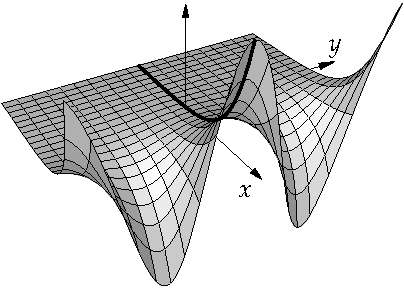
\includegraphics{figures/realexp}
\qquad
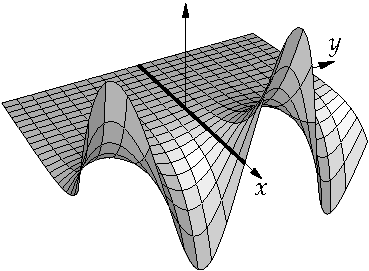
\includegraphics{figures/imagexp}
\caption{Grafik bagian real (kiri) dan bagian imajiner (kanan)
dari fungsi eksponensial kompleks $e^z = e^{x+iy}$.
Grafik fungsi eksponensial real ($y=0$)
ditandai dengan garis tebal.\label{fig:complexexpgraphs}}
\end{myfig}

Definisi tersebut sesuai dengan fungsi eksponensial standar untuk bilangan real (ketika
$y=0$).  Lebih lanjut,
\begin{equation*}
e^{\bar{z}} = 
e^{x-iy} =
e^x\cos y - i e^x \sin y  = \overline{e^{z}} ,
\end{equation*}
dan
\begin{equation*}
\sabs{e^{z}} = 
\sabs{e^{x+iy}} =
e^x .
\end{equation*}
Fungsi eksponensial kompleks dapat didefinisikan tanpa menggunakan
fungsi eksponensial real, sinus, dan kosinus, dan kelak kita akan melakukannya.
Namun, kita tidak sabar dan ingin memperoleh sesuatu untuk dicoba sekarang juga, tanpa menunggu.

\begin{prop}
Untuk sebarang dua bilangan kompleks $z,w \in \C$,
\begin{equation*}
e^{z+w} = e^z e^w .
\end{equation*}
\end{prop}

\begin{exbox}
\begin{exercise}%[\neededexmark]
Buktikan proposisi tersebut menggunakan definisi dan identitas trigonometri.
\end{exercise}
\end{exbox}

%We remark that $e^z$ is the unique continuous
%function on $\C$ that satisfies $e^{z+w} = e^z e^w$ and $\lim_{z\to
%0}\frac{1}{z}(e^z-1)=1$.
%Let us not worry about proving that.
Untuk $\theta$ real, definisi
fungsi eksponensial menghasilkan apa yang disebut
\emph{\myindex{rumus Euler}}:
\begin{equation*}
e^{i\theta}
=
\cos \theta + i \sin \theta .
\end{equation*}
Dengan kata lain, $e^{i \theta}$ memparametrisasi lingkaran satuan.
Rumus tersebut menyatakan bahwa untuk $\theta$ real,
\begin{equation*}
\cos \theta = \Re e^{i\theta} = \frac{e^{i\theta}+e^{-i\theta}}{2} ,
\qquad
\sin \theta = \Im e^{i\theta} = \frac{e^{i\theta}-e^{-i\theta}}{2i} .
\end{equation*}
Kita mendefinisikan kosinus dan sinus untuk bilangan kompleks dengan memasukkan
bilangan-bilangan tersebut
ke dalam rumus di atas, karena kini kita mengetahui cara menghitung fungsi eksponensial:
\begin{equation*}
\cos z \overset{\text{def}}{=} \frac{e^{iz}+e^{-iz}}{2} ,
\qquad
\sin z \overset{\text{def}}{=} \frac{e^{iz}-e^{-iz}}{2i} .
\end{equation*}

\subsection{Koordinat polar}

Karena bilangan kompleks tidak lain adalah bidang, kita dapat menggunakan
\emph{\myindex{koordinat polar}}
untuk merepresentasikan bilangan kompleks.
Artinya, $x = r \cos \theta$ dan $y= r \sin \theta$.
Kita menuliskan $z$ dalam \emph{\myindex{bentuk polar}} sebagai
\begin{equation*}
z = x+iy = r e^{i \theta} .
\end{equation*}
Di sini, $r = \sabs{z} = \sqrt{x^2+y^2}$ adalah modulus, dan
$\theta$ adalah sudut yang dibentuk $x+iy$ dengan sumbu real positif (sumbu-$x$).
Nilai $\theta$ disebut \emph{\myindex{argumen}}.  Lihat
\figureref{fig:polarcoords}.
Alasan penggunaan notasi tersebut adalah
rumus Euler, sehingga
\begin{equation*}
z = r e^{i\theta} = r\cos \theta + i r\sin \theta  = x+iy .
\end{equation*}

\begin{myfig}
\subimport*{figures/}{polarcoords.pdf_t}
\caption{Koordinat polar.\label{fig:polarcoords}}
\end{myfig}

Bentuk polar sangat baik digunakan untuk perkalian dan perpangkatan.
Misalkan $z = r e^{i\theta}$ dan $w = s e^{i \psi}$, maka
\begin{equation*}
zw =
r e^{i \theta} s e^{i \psi} = 
rs e^{i (\theta+ \psi)},
\qquad
\frac{1}{z} =
\frac{1}{r e^{i \theta}} =
\frac{1}{r} e^{-i \theta} ,
\qquad
z^n =
{\bigl(r e^{i \theta}\bigr)}^n =
r^n e^{i n\theta} .
\end{equation*}
Perkalian merotasi sebesar argumen dan mengubah skala sebesar modulus.
Secara khusus, kita kembali melihat bahwa perkalian dengan $i = e^{i \pi / 2}$ merupakan
rotasi berlawanan arah jarum jam sebesar $90$ derajat.
Kekurangannya adalah bahwa bentuk polar sangat buruk untuk penjumlahan.
Ada untung, ada rugi.

\begin{exbox}
\begin{exercise}
Misalkan $z,w$ adalah dua bilangan kompleks taknol dan misalkan
$\ell_z$ dan $\ell_w$ adalah sinar-sinar yang berpangkal di titik asal dan
masing-masing melalui
$z$ dan $w$.  Gunakan $\theta$ untuk menyatakan sudut antara $\ell_z$ dan
$\ell_w$.  Kemudian buktikan bahwa
$\Re z\bar{w} = \sabs{z} \sabs{w} \cos \theta$.
Perhatikan bahwa $\Re z\bar{w}$ adalah hasil kali titik real standar di $\R^2$, sehingga
Anda diminta membuktikan rumus hasil kali titik dari kalkulus.
\end{exercise}
\end{exbox}

\subsection{Argumen}

Kita mencoba mendefinisikan argumen dari $z = re^{i\theta}$ sebagai
\glsadd{not:arg}%
\begin{equation*}
\arg z
\overset{\text{def?}}{=}
\theta ,
\end{equation*}
tetapi kita menghadapi masalah bahwa jika $\theta$ merupakan suatu argumen dari $z$,
maka demikian pula $\theta+2\pi$, $\theta-2\pi$, atau $\theta + k 2\pi$ untuk sebarang
bilangan bulat $k$.  Dengan kata lain,
$\arg z$ bukanlah fungsi dalam pengertian klasik, melainkan
\emph{\myindex{fungsi bernilai banyak}}%
\footnote{Orang yang bukan analis kompleks kadang-kadang menyatakan bahwa fungsi bernilai banyak
tidak masuk akal, tetapi Anda dapat mengabaikan para pengacau itu dengan aman.}.  Definisi yang benar
adalah
\glsadd{not:arg}%
\begin{equation*}
\arg z
\overset{\text{def}}{=}
\ldots,\theta - 4\pi,
\theta - 2\pi,
\theta ,
\theta + 2\pi,
\theta + 4\pi, \ldots
\end{equation*}
Masih tersisa satu masalah kecil.  Jika $z=0$, maka $z=0=0 e^{i\theta}$ untuk sebarang
$\theta$.  Oleh karena itu, kita hanya mendefinisikan argumen untuk
$z$ taknol.

Kadang-kadang ada gunanya menetapkan satu bilangan tertentu sebagai argumen.
Kita mendefinisikan \emph{\myindex{cabang utama dari $\arg$}} sebagai
\glsadd{not:Arg}%
\begin{equation*}
\Arg z
\overset{\text{def}}{=}
\theta, \qquad \text{di mana } -\pi < \theta \leq \pi.
\end{equation*}
Ini mungkin tampak sebagai solusi yang baik bagi sifat bernilai banyak dari $\arg$, tetapi
harapan itu pupus oleh kenyataan pahit bahwa $\Arg$ tidak kontinu
pada sumbu real negatif.  Lihat \figureref{fig:arggraph}.
Cabang utama agak kurang berguna daripada yang mungkin dibayangkan.
Ada pula masalah bahwa tidak semua orang sepakat
mengenai arti \myquote{cabang utama}.
Sebagian matematikawan mengorbankan
sumbu real positif dan membiarkan $\theta$ berada dalam rentang $[0,2\pi)$.

\begin{myfig}
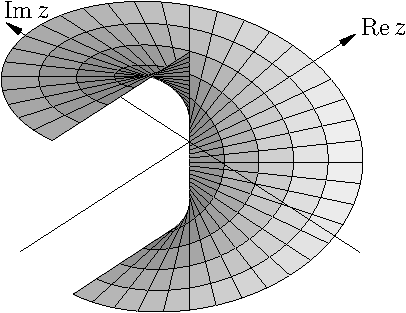
\includegraphics{figures/arggraph}
\caption{Grafik cabang utama argumen.\label{fig:arggraph}}
\end{myfig}

\begin{exbox}
\begin{exercise}
Tunjukkan bahwa $\Arg$ sebagaimana didefinisikan di atas bukan fungsi kontinu pada
$\C \setminus \{ 0 \}$.
\end{exercise}
\end{exbox}

\subsection{Sifat pemetaan fungsi eksponensial}

Mari kita lihat bagaimana fungsi eksponensial bekerja pada bidang kompleks.
Identitas $e^{z+w} = e^z e^w$ menyiratkan bahwa fungsi eksponensial
tidak pernah bernilai nol (latihan).
Dari sifat-sifat koordinat polar
dan fungsi eksponensial real yang telah diketahui, diperoleh bahwa fungsi eksponensial kompleks memetakan
secara surjektif ke $\C \setminus \{ 0 \}$.
Fungsi eksponensial kompleks tidak bersifat satu-ke-satu---setiap nilai memiliki
takhingga banyak prapeta.  Untuk sebarang bilangan bulat $k$,
\begin{equation} \label{eq:exponentialidentities}
e^{z+ik2\pi} = 
e^{z} e^{ik2\pi} =
e^z .
\end{equation}

\begin{exbox}
\begin{exercise} \label{exercise:exponetoonestrip}
Buktikan bahwa \eqref{eq:exponentialidentities} adalah satu-satunya identitas semacam itu dengan
menunjukkan bahwa jika $2k\pi < \Im z \leq 2(k+1)\pi$ dan
$2k\pi < \Im w \leq 2(k+1)\pi$, maka $e^z=e^w$ menyiratkan $z=w$.
\end{exercise}

\begin{exercise}%[\neededexmark]
Gunakan $e^{z+w} = e^z e^w$ dan $e^0 = 1 \neq 0$ untuk menunjukkan bahwa $e^z \neq 0$ untuk semua
$z \in \C$.  Dengan kata lain, tunjukkan bahwa jika suatu fungsi $f$ memenuhi $f(z+w)=f(z)f(w)$
dan $f(0) = 1$, maka $f(z) \neq 0$ untuk semua $z$.
\end{exercise}
\end{exbox}

Tinjau garis vertikal yang diberikan oleh $x=c$.  Karena
\begin{equation*}
e^{z} = 
e^{x+iy} =
e^x e^{iy}
\end{equation*}
dan $\sabs{e^{iy}} =1$, fungsi eksponensial memetakan garis vertikal $x=c$ ke
lingkaran berjari-jari $e^c$.  Lihat \figureref{fig:expplotlines}.
Dengan demikian, fungsi eksponensial $w=e^z$ memetakan pita $a < x < b$ ke
anulus
\begin{equation*}
\bigl\{ w \in \C : e^a < \sabs{w} < e^b \bigr\} .
\end{equation*}

Di sisi lain, garis horizontal $y=c$
dipetakan ke sinar dari titik asal menuju takhingga dengan $\theta = c$ dalam
koordinat polar.  Lihat kembali \figureref{fig:expplotlines}.
Oleh karena itu, fungsi eksponensial memetakan pita $a < y < b$ ke
sektor
\begin{equation*}
\bigl\{ w \in \C : ``a < \arg w < b'' \bigr\} .
\end{equation*}
Tanda kutip digunakan karena pertidaksamaan tersebut tidak
bermakna tanpa penafsiran yang tepat.  Maksudnya, setidaknya salah satu nilai
dari $\arg w$ berada di antara $a$ dan $b$.
Secara khusus, fungsi eksponensial $e^z$ memetakan himpunan yang diberikan oleh
$2k\pi < \Im z \leq 2(k+1)\pi$ secara satu-ke-satu
(lihat \exerciseref{exercise:exponetoonestrip})
ke $\C \setminus \{ 0 \}$.

\begin{myfig}
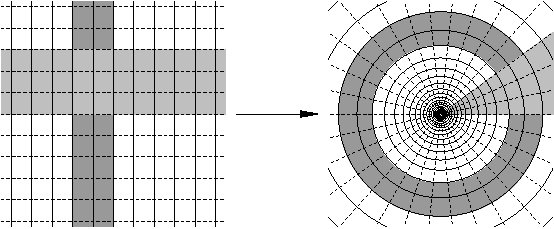
\includegraphics{figures/expplotlines}
\caption{Garis horizontal dan vertikal, serta sebuah pita horizontal dan sebuah pita
vertikal, yang dipetakan oleh fungsi eksponensial.  Perhatikan bahwa
setiap garis horizontal hanya dipetakan ke suatu sinar dari
titik asal.\label{fig:expplotlines}}
\end{myfig}

%%%%%%%%%%%%%%%%%%%%%%%%%%%%%%%%%%%%%%%%%%%%%%%%%%%%%%%%%%%%%%%%%%%%%%%%%%%%%%

\section{Bola Riemann}

Kadang-kadang berguna untuk memperluas bilangan real dengan menambahkan $\pm \infty$.
Konsep serupa tersedia untuk bidang kompleks, meskipun
kita hanya menambahkan satu takhingga.  Kita menulis
\glsadd{not:Cinfty}%
\glsadd{not:infty}%
\begin{equation*}
\C_{\infty} = \C \cup \{ \infty \} ,
\end{equation*}
dan kita menyebut $\C_{\infty}$ sebagai \emph{\myindex{bola Riemann}}.
Kita menginginkan topologi $\C_\infty$ sama dengan topologi $\C$
ketika jauh dari takhingga.
Definisikan fungsi $g \colon \C_\infty \to \C_\infty$ dengan
\begin{equation*}
g(z) =
\begin{cases}
\nicefrac{1}{z} & \text{jika } z \neq 0 \text{ dan } z \neq \infty, \\
\infty & \text{jika } z = 0, \\
0 & \text{jika } z = \infty.
\end{cases}
\end{equation*}
Fungsi $g$ bersifat bijektif (satu-ke-satu dan surjektif).
Setiap lingkungan titik asal dalam $\C$ dipetakan ke suatu himpunan yang
memuat takhingga, dan himpunan semacam itu kita sebut lingkungan
$\infty$.  Ketika membicarakan lingkungan
takhingga dalam $\C_{\infty}$, yang sebenarnya ingin kita pikirkan adalah pemetaan ini
dan lingkungan titik asal yang bersesuaian.

Secara lebih konkret, kita dapat memberi $\C_{\infty}$ struktur ruang metrik.
Misalkan $S^2$ adalah bola satuan dalam $\R^3$,
yakni himpunan yang dinyatakan oleh $x^2 + y^2 + z^2 = 1$ jika $(x,y,z)$ adalah
koordinatnya.\footnote{Paragraf ini mungkin merupakan satu-satunya bagian dalam buku ini tempat
$z$ merupakan bilangan real.}  Bidang $\R^2$ dengan koordinat $(x,y)$ dapat
diidentifikasikan dengan $\C$ berkoordinat $\xi$ dengan mengambil $x+iy = \xi$.
Diberikan sebarang titik $p \in S^2$ yang bukan kutub utara $(0,0,1) \in S^2$,
terdapat tepat satu garis dalam $\R^3$ yang melalui titik $(0,0,1)$ dan $p$.
Tidak sulit membuktikan bahwa garis ini tidak pernah sejajar dengan
bidang-$xy$, yakni dengan $\C$, sehingga garis tersebut harus memotong $\C$ di tepat satu
titik $\xi \in \C$ (suatu bidang dan garis berpotongan di tepat satu titik kecuali
keduanya sejajar).  Definisikan
\begin{equation*}
\Phi(p) = \xi.
\end{equation*}
Tetapkan $\Phi\bigl((0,0,1)\bigr) = \infty$, sehingga kita memperoleh pemetaan
$\Phi \colon S^2 \to \C_\infty$.  Pemetaan ini disebut
\emph{\myindex{proyeksi stereografik}}.  Lihat
\figureref{fig:riemannsphere}.
Pemetaan tersebut bijektif (latihan di bawah),
sehingga definisikan metrik pada $\C_\infty$ dengan
menggunakan metrik pada $S^2$, yang dapat berupa metrik
subruang yang berasal dari metrik Euklides pada $\R^3$.
Kemungkinan lain
adalah jarak lingkaran besar, \exampleref{ms:greatcircle}.
Kedua jarak tersebut menghasilkan topologi yang sama, dan dengan demikian limit yang sama.

\begin{myfig}
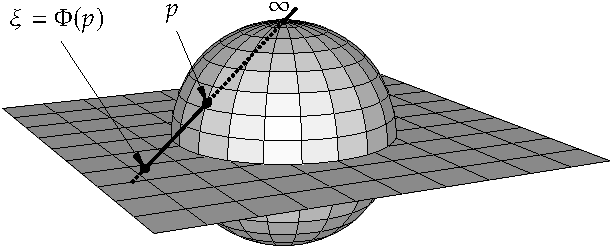
\includegraphics{figures/riemannsphere}
\caption{Proyeksi stereografik bola $S^2$ ke bidang
kompleks.\label{fig:riemannsphere}}
\end{myfig}

\begin{exbox}
\begin{exercise}%[\neededexmark]
Tunjukkan bahwa $\Phi$ bijektif.
\end{exercise}

\begin{exercise}
Misalkan $(\phi,\theta)$
adalah koordinat sferis pada $S^2$, dengan $0 \leq \phi \leq \pi$ sebagai zenit (sudut yang dibentuk
dengan sumbu-$z$) dan $-\pi < \theta \leq \pi$ sebagai azimut, dan kita menuliskan
titik-titik dalam $\C$ menggunakan koordinat polar $re^{i\theta}$.  Kemudian buktikan bahwa
$\Phi$ memetakan
$(\phi,\theta)$ ke $\cot (\nicefrac{\phi}{2})\,e^{i\theta}$.
\end{exercise}

\begin{exercise}%[\neededexmark]
Tunjukkan bahwa topologi pada $\C$ yang diinduksi oleh topologi $S^2$ menggunakan $\Phi$
seperti di atas ekuivalen dengan topologi standar.  Artinya, tunjukkan bahwa suatu himpunan $U
\subset \C$
terbuka dalam metrik Euklides pada $\C$ jika dan hanya jika terbuka dalam
metrik yang berasal dari $S^2$.
\end{exercise}
\end{exbox}

Tujuan bola Riemann adalah memberikan nilai $\infty$ kepada limit-limit
tertentu dan memungkinkan limit ketika $z$ menuju $\infty$.  Untuk suatu
fungsi $f \colon U \subset \C_\infty \to \C_\infty$, kita mendefinisikan
\begin{equation*}
\lim_{z \to z_0} f(z) = L
\end{equation*}
sebagai limit dengan menggunakan topologi pada bola Riemann,
termasuk
kasus ketika $z_0 = \infty$, $L = \infty$, atau keduanya.
Untungnya, bola Riemann bersifat kompak.
Secara topologis, bola ini memang sama dengan
\myquote{kompaktifikasi satu titik} dari $\C$.

\begin{exbox}
\begin{exercise}%[\neededexmark]
Misalkan $L \in \C$ dan $z_0 \in \C$.
Tunjukkan bahwa $\lim_{z\to z_0} f(z) = L$ dalam pengertian bola Riemann
jika dan hanya jika $\lim_{z \to z_0} f(z) = L$ dalam pengertian biasa (metrik Euklides
pada $\C$).
\end{exercise}

\begin{exercise}%[\neededexmark]
Misalkan $L \in \C$.
Tunjukkan bahwa $\lim_{z\to \infty} f(z) = L$ dalam pengertian bola Riemann
jika dan hanya jika untuk setiap $\epsilon > 0$ terdapat $M$ sedemikian sehingga
$\sabs{f(z)-L} < \epsilon$ setiap kali $z \in \C$ dan $\sabs{z} > M$.
\end{exercise}

\begin{exercise}%[\neededexmark]
Misalkan $z_0 \in \C$.
Tunjukkan bahwa $\lim_{z\to z_0} f(z) = \infty$ dalam pengertian bola Riemann
jika dan hanya jika untuk setiap $M > 0$ terdapat $\delta > 0$ sedemikian sehingga
$\sabs{f(z)} > M$ setiap kali $0 < \sabs{z-z_0} < \delta$.
\end{exercise}

\begin{exercise}%[\neededexmark]
Misalkan $L \in \C_\infty$.
Tunjukkan bahwa $\lim\limits_{z\to\infty} f(z) = L$ jika dan hanya jika
$\lim\limits_{z \to 0} f(\nicefrac{1}{z}) = L$.
\end{exercise}

\begin{exercise}%[\neededexmark]
Misalkan $z_0 \in \C_\infty$.
Tunjukkan bahwa $\lim\limits_{z\to z_0} f(z) = \infty$ jika dan hanya jika
$\lim\limits_{z \to z_0} \frac{1}{f(z)} = 0$.
\end{exercise}
\end{exbox}

Dengan demikian, masuk akal membicarakan nilai $\nicefrac{1}{z}$ di titik asal
sebagai $\infty$, dan nilai $z$ pada $\infty$ sebagai $\infty$.
Bahkan, setiap polinom takkonstan bernilai $\infty$ pada $\infty$.

\begin{exbox}
\begin{exercise}%[\neededexmark]
\label{exercise:polygoesinf}
Misalkan $P(z) = a_d z^d + a_{d-1} z^{d-1} + \cdots + a_1 z + a_0$ adalah
polinom dengan $a_0,\ldots,a_d \in \C$.  Buktikan bahwa jika $d \geq 1$
dan $a_d \neq 0$ ($P$ takkonstan),
maka $\lim_{z \to \infty} P(z) = \infty$.
Petunjuk: Jika $a_d = 1$, maka dengan menggunakan
$\abs{\frac{a_{d-1} z^{d-1} + \cdots + a_1 z + a_0}{z^d}}$, diperoleh
$\abs{P(z)} \geq \frac{1}{2} \sabs{z}^d$ untuk $z$ yang besar.
\end{exercise}
\end{exbox}

Dalam kalkulus dan analisis real dasar, Anda mungkin pernah menjumpai
limit takhingga dalam pengertian bilangan real diperluas.
Walaupun kedua jenis limit takhingga tersebut, baik dalam pengertian
bilangan real diperluas maupun dalam pengertian bola Riemann,
tampak serupa dan pada dasarnya menggunakan notasi yang sama,
keduanya berbeda.
Sebagai contoh,
\begin{equation*}
\lim_{x \to 0} \frac{1}{x} \quad \text{tidak ada,} \qquad \text{tetapi} \qquad
\lim_{z \to 0} \frac{1}{z} = \infty .
\end{equation*}
Di sini, pada ruas kiri kita secara diam-diam menggunakan pengertian real diperluas
($x$ real, bukan?) dan pada
ruas kanan kita secara diam-diam menggunakan pengertian bola Riemann ($z$ tampaknya kompleks).
Asumsi implisit semacam itu jelas dapat menimbulkan kebingungan.
Dalam buku ini, limit akan dipahami dalam pengertian bola Riemann
kecuali dinyatakan lain atau sudah jelas.
Jika kebingungan mungkin timbul, kita akan menulis $\infty$ real diperluas
sebagai $+\infty$.

\medskip

Aritmetika (parsial) yang dapat
didefinisikan secara wajar dengan $\infty$ pada bola Riemann
cukup berbeda dari
$\infty$ pada bilangan real diperluas.
Untuk $c \neq \infty$, kita dapat mendefinisikan $c+\infty = \infty$,
tetapi baik $\infty+\infty$ maupun $\infty-\infty$ tidak bermakna.
Sebagai contoh, jika $f(z) = z$ dan $g(z) = c-z$,
maka $\lim_{z \to \infty} f(z) = \infty$,
$\lim_{z \to \infty} g(z) = \infty$, tetapi $\lim_{z \to \infty}
\bigl(f(z)+g(z)\bigr) = c$, sehingga $\infty+\infty$ tidak bermakna.
Berbeda dengan bilangan real diperluas,
masuk akal (dan kadang berguna) untuk mendefinisikan $\nicefrac{c}{0} = \infty$ bagi
$c \neq 0$, $\nicefrac{c}{\infty} = 0$ bagi $c \neq \infty$,
dan $c \cdot \infty = \infty$ bagi $c \neq 0$.
%We could also define $\infty \cdot \infty = \infty$, $\frac{0}{\infty} = 0$,
%and
%$\frac{\infty}{0} = \infty$.
Ekspresi $0 \cdot \infty$, $\nicefrac{0}{0}$, dan
$\nicefrac{\infty}{\infty}$ sebaiknya dibiarkan tak terdefinisi.

%%%%%%%%%%%%%%%%%%%%%%%%%%%%%%%%%%%%%%%%%%%%%%%%%%%%%%%%%%%%%%%%%%%%%%%%%%%%%%

\section{Transformasi pecahan linear}

\emph{Transformasi pecahan linear}\index{transformasi pecahan linear}
(LFT)\index{LFT}
(kadang disebut \emph{\myindex{transformasi M\"obius}})
merupakan sekumpulan transformasi yang praktis pada bidang kompleks atau bola
Riemann.
Suatu fungsi
\begin{equation*}
f(z) = \frac{a z + b}{c z + d}
\end{equation*}
adalah transformasi pecahan linear jika $ad \neq bc$.  Syarat pada
$a$, $b$, $c$, $d$ menjamin bahwa rasio tersebut tidak dapat disederhanakan dan bahwa
fungsinya tidak konstan.

Jika $c \neq 0$,
ekspresi tersebut sebenarnya hanya terdefinisi pada
$\C \setminus \bigl\{ \nicefrac{-d}{c} \bigr\}$;
namun, seperti pada bagian sebelumnya, kita tulis
\begin{equation*}
f\left(\frac{-d}{c}\right) = \infty, \qquad \text{dan} \qquad
f(\infty) = \frac{a}{c} .
\end{equation*}
Jika $c=0$, tetapkan $f(\infty) = \infty$.  Dalam kedua kasus, $f$ adalah pemetaan
bola Riemann ke dirinya sendiri.

\begin{exbox}
\begin{exercise}%[\neededexmark]
Buktikan bahwa LFT merupakan pemetaan bijektif bola Riemann ke dirinya sendiri.
\end{exercise}

\begin{exercise}%[\neededexmark]
Buktikan bahwa LFT yang diperluas ke bola Riemann seperti di atas bersifat kontinu.
\end{exercise}
\end{exbox}

Setiap LFT merupakan komposisi dari \emph{translasi}\index{translasi}
\begin{equation*}
T_a(z) = z + a , \qquad a \in \C,
\end{equation*}
\emph{dilatasi kompleks}\index{dilatasi kompleks}
\begin{equation*}
D_a(z) = az , \qquad a \in \C \setminus \{ 0 \} ,
\end{equation*}
dan \emph{inversi}\index{inversi}
\begin{equation*}
I(z) = \frac{1}{z}.
\end{equation*}
Perhatikan suatu LFT $f(z) = \frac{az+b}{cz+d}$.
Tanpa mengurangi keumuman, andaikan bahwa $c=1$ atau $c=0$.
Pertama, misalkan $c=1$,
\begin{equation*}
f(z)
=
\frac{a z + b}{z + d}
=
\frac{b-ad}{z+d}+a
=
T_a\biggr(D_{b-ad}\Bigl(I\bigl(T_d(z)\bigr)\Bigr)\biggr) .
\end{equation*}
Jika $c=0$, kita juga dapat mengandaikan bahwa $d=1$ dan
dengan demikian $f(z) = az + b$.  Jadi
\begin{equation*}
f(z) = az+b = T_b\bigl(D_a(z)\bigr) .
\end{equation*}

Translasi mudah dipahami.
Translasi memindahkan segala sesuatu dalam $\C$ ke satu arah.
Dilatasi
kompleks $D_a$ adalah dilatasi geometri bidang Euklides biasa dengan faktor $\sabs{a}$
dan rotasi sebesar $\arg a$.
Inversi adalah inversi geometri bidang Euklides
terhadap lingkaran satuan
disertai konjugasi kompleks.  Lihat \figureref{fig:inversion}.  Inversi Euklides
terhadap lingkaran hanya membalikkan jarak ke titik asal:
\begin{equation*}
\frac{1}{\sabs{z}} e^{i \arg z} = 
\frac{\sabs{z}}{\sabs{z}^2} e^{i \arg z} = \frac{1}{\bar{z}} .
\end{equation*}
Untuk memperoleh inversi kompleks kita $I(z)$, kita juga melakukan konjugasi.
Translasi dan dilatasi sama-sama memetakan $\infty$ ke $\infty$.
Inversi mempertukarkan $\infty$ dan $0$.

\begin{myfig}
\subimport*{figures/}{inversion.pdf_t}
\caption{Inversi kompleks.\label{fig:inversion}}
\end{myfig}

Dekomposisi semacam ini cukup berguna untuk membuktikan pernyataan tentang
LFT yang dipertahankan oleh komposisi;
kita hanya perlu membuktikannya untuk $T_a$, $D_a$, dan $I$.  Teknik ini
akan langsung berguna dalam latihan berikutnya.
Mari kita sertakan garis lurus dalam himpunan lingkaran.  Bagaimanapun, garis
lurus hanyalah lingkaran yang melalui tak hingga: Bayangkan lingkaran berjari-jari $r$
yang berpusat di $ir$ saat $r \to +\infty$.  Maka LFT memetakan lingkaran ke lingkaran.
Fakta ini kita serahkan sebagai latihan.

\begin{exbox}
\begin{exercise}
Buktikan bahwa jika kita menyertakan garis lurus dalam himpunan \myquote{lingkaran,} maka
LFT memetakan lingkaran ke lingkaran.
\end{exercise}

\begin{exercise} \label{exercise:anycircletorealline}
Buktikan bahwa untuk setiap lingkaran atau garis lurus, terdapat LFT
yang memetakan lingkaran atau garis tersebut ke garis real.
\end{exercise}
\end{exbox}

Salah satu cara memandang LFT adalah sebagai matriks kompleks $2 \times 2$.  Untuk tujuan
ini,
kita perlu memandang bola Riemann sebagai apa yang disebut
\emph{\myindex{ruang proyektif}} satu dimensi (kompleks)\index{ruang proyektif kompleks}.
Definisikan relasi ekuivalensi $\sim$ pada
$\C^2 \setminus \{ 0 \} = \C \times \C \setminus \{ (0,0) \}$ dengan
$u \sim v$ jika dan hanya jika $u = \lambda v$ untuk suatu $\lambda \in \C \setminus
\{ 0 \}$.
Ruang proyektif kompleks satu dimensi
kemudian didefinisikan sebagai ruang hasil bagi
\glsadd{not:CP1}%
\begin{equation*}
\C \bP^1
\overset{\text{def}}{=}
\faktor{\C^2 \setminus \{ 0\}}{\sim} \ .
\end{equation*}
Dengan kata lain, $\C \bP^1$ adalah himpunan \myquote{garis kompleks yang melalui
titik asal} di $\C^2$, atau dengan ungkapan lain lagi,
ia adalah himpunan subruang vektor satu dimensi
dari $\C^2$.

Kita identifikasikan $\C\bP^1$ dengan $\C_\infty$ dengan cara
berikut.  Nyatakan dengan
\glsadd{not:CP1pt}%
$[z:w] \in \C \bP^1$
kelas ekuivalensi (terhadap $\sim$) dari vektor-vektor dalam $\C^2 \setminus \{0\}$
yang memuat $(z,w) \in \C^2 \setminus \{0\}$.
Definisikan bijeksi $\Psi \colon \C_\infty \to \C \bP^1$ dengan
\begin{equation*}
\Psi(z) =
\begin{cases}
[z:1] & \text{jika } z \in \C , \\
[1:0] & \text{jika } z=\infty .
\end{cases}
\end{equation*}

\begin{exbox}
\begin{exercise}
Buktikan bahwa $\Psi$ yang didefinisikan di atas bersifat bijektif.
\end{exercise}
\end{exbox}

Mari kita periksa bahwa suatu LFT
\begin{equation*}
f(z) = \frac{a z + b}{c z + d}
\end{equation*}
bersesuaian dengan suatu pemetaan linear invertibel yang diberikan oleh matriks
\begin{equation*}
M =
\begin{bmatrix}
a & b \\
c & d
\end{bmatrix} .
\end{equation*}
Matriks invertibel $M$ memetakan subruang satu dimensi ke subruang satu dimensi,
jadi hal ini terdengar masuk akal.

Pertama, $\Psi \circ f$ untuk $z \in \C \setminus \bigl\{ \nicefrac{-d}{c} \bigr\}$
(atau $z \in \C$ jika $c=0$)
sama dengan
\begin{equation*}
\Psi \circ f(z) =
\left[\frac{a z + b}{c z + d}: 1 \right]
=
\left[a z + b: c z + d \right] ,
\end{equation*}
di mana kesamaan kedua mengikuti dari definisi $\sim$.
Ketika $z = \nicefrac{-d}{c}$, maka $cz+d = 0$, dan
$\Psi\circ f(z) = \Psi(\infty) = [1:0] = [az+b : cz+d]$ juga.

Mari kita tinjau $\Psi \circ f \circ \Psi^{-1}$.
Jika $w \neq 0$, maka $[z:w] = [ \nicefrac{z}{w}:1 ]$.  Jadi
\begin{equation*}
\Psi \circ f \circ \Psi^{-1} \bigl([z:w]\bigr) =
\Psi \circ f \left(\frac{z}{w}\right) =
\left[a \frac{z}{w} + b : c \frac{z}{w} + d \right] =
\left[a z + b w: c z + d w \right] .
\end{equation*}
Dan dapat diperiksa bahwa kesamaan yang sama berlaku jika $w=0$.
Karena
$M \left[ \begin{smallmatrix} z \\ w \end{smallmatrix} \right]
= \left[ \begin{smallmatrix} 
a z + b w \\ c z + d w
\end{smallmatrix} \right]$,
fungsi $f$ bersesuaian dengan pemetaan linear $v \mapsto Mv$ pada $\C^2$.
Syarat $ad \neq bc$ mengakibatkan $\det M \neq 0$,
atau dengan kata lain, $M$ invertibel.
Jadi setiap LFT direpresentasikan oleh suatu matriks invertibel $2 \times 2$, $M$
(tidak secara unik), dan
sebaliknya setiap matriks invertibel $2 \times 2$, $M$, bersesuaian dengan suatu LFT\@.

Suatu matriks invertibel $2 \times 2$, $M$, memberikan pemetaan dari
$\C^2 \setminus \{ 0 \}$ ke $\C^2 \setminus \{ 0 \}$.
Misalkan $\pi \colon \C^2 \setminus \{ 0 \} \to \C \bP^1$ adalah pemetaan\footnote{Yang
\myquote{pemetaan hasil bagi} atau \myquote{proyeksi alami.}}
$\pi \bigl( (z,w) \bigr) =
[z:w]$.  Diagram komutatif berikut\footnote{Sebuah diagram bersifat
komutatif jika menempuh dua lintasan berbeda dalam gambar
menghasilkan pemetaan yang sama.}
mungkin
menggambarkan keseluruhan situasi dengan lebih baik:
\begin{equation*}
\begin{tikzcd}
\C^2 \setminus \{ 0 \} \arrow[r,"M"] \arrow[d,"\pi"] &
\C^2 \setminus \{ 0 \} \arrow[d,"\pi"] \\
\C \bP^1 \arrow[r,"\Psi \circ f \circ \Psi^{-1}"] \arrow[d,shift left,"\Psi^{-1}"] &
\C \bP^1 \arrow[d,shift left,"\Psi^{-1}"]
\\
\C_\infty \arrow[r,"f"]\arrow[u,shift left,"\Psi"] &
\C_\infty \arrow[u,shift left,"\Psi"]
\end{tikzcd}
\end{equation*}

\begin{example}
Salah satu LFT yang praktis adalah
\emph{\myindex{pemetaan Cayley}}:
\begin{equation*}
C(z)
=
\frac{z - i}{z + i} .
\end{equation*}
Pemetaan ini jelas merupakan LFT\@, dan
memetakan setengah bidang atas $\bH = \{ z \in \C : \Im z > 0 \}$ ke
cakram satuan $\D$.  Mari kita lihat alasannya.  Pemetaan tersebut memetakan $z \in \C$ ke cakram satuan jika
\begin{equation*}
1 > \abs{\frac{z - i}{z + i} }
=
\frac{\sabs{z - i}}{\sabs{z + i}} .
\end{equation*}
Dengan kata lain, $\sabs{z+i} > \sabs{z - i}$: Jarak dari $z$
ke $-i$ lebih besar daripada jarak dari $z$ ke $i$.  Dari geometri bidang
langsung terlihat bahwa $z \in \bH$.  Lihat
\figureref{fig:cayleydisc}.
\begin{myfig}
\subimport*{figures/}{cayleydisc.pdf_t}
\caption{Mengapa pemetaan Cayley memetakan $\bH$ ke $\D$.\label{fig:cayleydisc}}
\end{myfig}
\end{example}

Setiap LFT bersifat bijektif jika dipandang sebagai pemetaan dari $\C_\infty$
ke dirinya sendiri, sehingga $C^{-1}$ ada, dan ia juga merupakan pemetaan yang berguna.  Kita serahkan
sebagai latihan untuk menentukan inversnya.

\begin{exbox}
\begin{exercise}
Tentukan $C^{-1}$ (invers Cayley).  Petunjuk: Pandang $\C_\infty$ sebagai $\C \bP^1$
dan $C$ sebagai matriks.  Matriks $2 \times 2$ sangat mudah diinverskan.
\end{exercise}

\begin{exercise}
Untuk setiap LFT $f(z) = \frac{az+b}{cz+d}$, tentukan $f^{-1}$.
Petunjuk: Petunjuk yang sama seperti di atas.
\end{exercise}
\end{exbox}

Dalam latihan-latihan tersebut, pada dasarnya Anda baru saja menunjukkan (atau setidaknya menyelesaikan
pembuktian) bahwa LFT membentuk suatu grup terhadap komposisi,
yang disebut \emph{\myindex{grup M\"obius}}.
Grup ini dibangkitkan oleh elemen-elemen
$T_a$, $D_b$, dan $I$ untuk $a\in \C$, $b \in \C \setminus \{ 0 \}$.

%%%%%%%%%%%%%%%%%%%%%%%%%%%%%%%%%%%%%%%%%%%%%%%%%%%%%%%%%%%%%%%%%%%%%%%%%%%%%%

\section{Rasio silang \texorpdfstring{$\star$}{*}}

Ada suatu besaran yang dipertahankan oleh LFT, yaitu
\emph{\myindex{rasio silang}}:
\glsadd{not:crossratio}%
\begin{equation*}
(z_1,z_2;z_3,z_4)
=
\frac{(z_3-z_1)(z_4-z_2)}{(z_3-z_2)(z_4-z_1)}
=
\frac{z_3-z_1}{z_3-z_2} : 
\frac{z_4-z_1}{z_4-z_2} ,
\end{equation*}
di mana $z_1,z_2,z_3,z_4$ adalah bilangan kompleks.  Rasio silang
sudah dideskripsikan oleh bangsa Yunani kuno\footnote{Oleh
Pappus dari Aleksandria, yang
hidup pada awal abad ke-4 Masehi\@.  Jadi, ini tidak setua dan semengesankan,
misalnya,
teorema Thales dari sekitar seribu tahun sebelumnya.  Lagi pula, bukankah
Aleksandria berada di Mesir?}
dan memainkan peran utama dalam geometri proyektif.
Definisi ini diperluas ke kasus ketika salah satu bilangannya adalah $\infty$ dengan cukup
menghapus suku-suku yang terpengaruh dari rasio.  Sebagai contoh, jika $z_1=\infty$,
anggaplah bahwa $z_3-\infty$
sebenarnya sama dengan $z_4-\infty$ dan
dengan demikian keduanya saling menghapus---yang masuk akal karena $\lim_{z\to\infty} \frac{z_3-z}{z_4-z} = 1$.
Akibatnya,
\begin{align*}
(\infty,z_2;z_3,z_4)
& =
\frac{z_4-z_2}{z_3-z_2}
,
&
(z_1,\infty;z_3,z_4)
& =
\frac{z_3-z_1}{z_4-z_1}
,
\\
(z_1,z_2;\infty,z_4)
& =
\frac{z_4-z_2}{z_4-z_1}
,
& 
(z_1,z_2;z_3,\infty)
& =
\frac{z_3-z_1}{z_3-z_2} .
\end{align*}

Dengan \myquote{dipertahankan oleh LFT,} yang kita maksud adalah:

\begin{prop} \label{prop:crossratioinvariant}
Andaikan $f$ adalah suatu LFT\@.  Maka
\begin{equation*}
(z_1,z_2;z_3,z_4) =
\bigl(f(z_1),f(z_2);f(z_3),f(z_4)\bigr) .
\end{equation*}
\end{prop}

\begin{exbox}
\begin{exercise}
Buktikan \propref{prop:crossratioinvariant}.
\end{exercise}

\begin{exercise}
Buktikan bahwa empat titik yang berbeda terletak pada satu garis atau satu lingkaran jika dan hanya jika
rasio silangnya real.
Petunjuk: Lihat juga \exerciseref{exercise:anycircletorealline}.
\end{exercise}
\end{exbox}

Rasio silang memberikan cara yang praktis untuk mendeskripsikan LFT.
Untuk tiga bilangan berbeda $z_2,z_3,z_4$, fungsi
\begin{equation*}
f(z) =
(z,z_2;z_3,z_4)
\end{equation*}
adalah LFT sedemikian sehingga $f(z_2) = 1$, $f(z_3)=0$ dan $f(z_4) = \infty$.
Dengan kata lain,
$(z,z_2;z_3,z_4) = 
\bigl(f(z),1;0,\infty\bigr)$.

\begin{exbox}
\begin{exercise}
Diberikan dua tripel titik berbeda $z_1,z_2,z_3 \in \C_\infty$
dan $w_1,w_2,w_3 \in \C_\infty$, tentukan secara eksplisit suatu LFT $f$
sedemikian sehingga
$f(z_1) = w_1$,
$f(z_2) = w_2$, dan
$f(z_3) = w_3$.
\end{exercise}

\begin{exercise}
Diberikan titik-titik berbeda $z_1,z_2,z_3 \in \C$ dan
dengan menggunakan definisi rasio silang untuk LFT\@, tentukan secara eksplisit
persamaan lingkaran (atau garis lurus) yang melalui ketiga titik tersebut.
Petunjuk: Pracitra garis real adalah lingkaran atau garis lurus.
\end{exercise}
\end{exbox}


%%%%%%%%%%%%%%%%%%%%%%%%%%%%%%%%%%%%%%%%%%%%%%%%%%%%%%%%%%%%%%%%%%%%%%%%%%%%%%
%%%%%%%%%%%%%%%%%%%%%%%%%%%%%%%%%%%%%%%%%%%%%%%%%%%%%%%%%%%%%%%%%%%%%%%%%%%%%%
%%%%%%%%%%%%%%%%%%%%%%%%%%%%%%%%%%%%%%%%%%%%%%%%%%%%%%%%%%%%%%%%%%%%%%%%%%%%%%
\chapter{Fungsi Holomorfik dan Analitik} \label{ch:holanal}

\begin{myepigraph}
Jika ini kopi, tolong bawakan saya teh; tetapi jika ini teh, tolong bawakan saya kopi.

---Abraham Lincoln
\end{myepigraph}

%%%%%%%%%%%%%%%%%%%%%%%%%%%%%%%%%%%%%%%%%%%%%%%%%%%%%%%%%%%%%%%%%%%%%%%%%%%%%%

\section{Fungsi holomorfik dan Cauchy--Riemann}
\label{sec:holfuncs}

\subsection{Fungsi holomorfik}

Fungsi yang ingin kita pelajari adalah fungsi yang dalam arti tertentu
memperumum polinomial dalam $z \in \C$; kita ingin mempelajari fungsi
yang,
setidaknya secara lokal, berperilaku seperti $P(z) = a_n z^n + a_{n-1} z^{n-1} + \cdots +
a_1 z + a_0$.  Polinomial mudah dipahami dan mudah digunakan.
Sayangnya, jumlahnya tidak begitu banyak.  Sebagai contoh, tidak ada
polinomial taknol yang menyelesaikan persamaan diferensial paling dasar: $f' =
f$.  Kita harus sedikit memperluas cakrawala.

Perhatikan suatu polinomial $P(z)$ dan kembangkan di sekitar suatu $z_0 \in \C$:
\begin{equation*}
P(z) = c_0 + c_1 (z-z_0) + c_2 {(z-z_0)}^2 + \cdots + c_n {(z-z_0)}^n .
\end{equation*}
Dengan kata lain, $P(z_0+h) = c_0 + c_1 h + c_2 h^2 + \cdots + c_n h^n$.
Maka
\begin{equation*}
\lim_{h \to 0} \frac{P(z_0+h) - P(z_0)}{h} =
\lim_{h \to 0} \frac{P(z_0+h) - c_0}{h} = c_1 .
\end{equation*}
Jadi $P(z_0+h)$ dihampiri (secara lokal) oleh $c_0 + c_1 h$
dengan galat yang menuju nol lebih cepat daripada $h$.
Perlu kita tekankan bahwa limit tersebut diambil \myquote{ketika $h$ yang \emph{kompleks}
menuju $0$.}

Karena itu, kita ingin mempelajari fungsi yang secara lokal
dihampiri oleh $c_0 + c_1 h$ dengan cara yang sama.  Secara lebih formal,
kita menginginkan fungsi sedemikian sehingga
\begin{equation*}
f(z_0+h) = \underbrace{f(z_0)}_{c_0} + \underbrace{\xi h}_{c_1 h} + o(\sabs{h})
\end{equation*}
untuk suatu $\xi \in \C$, dengan
\glsadd{not:oofh}%
$o(\sabs{h})$ berarti sebarang
fungsi $\varphi(h)$ sedemikian sehingga
$\lim_{h\to0} \frac{\varphi(h)}{\sabs{h}} = 0$.
% function of $h$ that goes to zero faster than $\sabs{h}$.

\begin{defn}
Andaikan $U \subset \C$ terbuka.
Diberikan $f \colon U \to \C$ dan $z_0 \in U$, kita katakan
$f$ \emph{\myindex{terdiferensial secara kompleks}} di $z_0$ jika
limit
\glsadd{not:cplxder}%
\begin{equation} \label{eq:complexdiff}
f'(z_0) \overset{\text{def}}{=}
\lim_{h \to 0} \frac{f(z_0+h) - f(z_0)}{h} \qquad ( = \xi )
\end{equation}
ada.
Kita menyebut $f'(z_0)$ sebagai \emph{\myindex{turunan kompleks}} dari $f$
di $z_0$.  Notasi
\glsadd{not:cplxderalt}%
 $\frac{df}{dz}$ juga berguna.

Suatu fungsi $f \colon U \to \C$ disebut
\emph{\myindex{holomorfik}}
jika ia terdiferensial secara kompleks di setiap titik.  Artinya, jika
\eqref{eq:complexdiff} ada untuk semua $z_0 \in U$.
\end{defn}

Di atas, kita membuktikan proposisi berikut, yang membenarkan motivasi kita
untuk turunan kompleks.

\begin{prop}
Jika $P(z)$ adalah polinomial, maka $P \colon \C \to \C$ holomorfik.
\end{prop}

Hasil paling mendasar tentang fungsi holomorfik adalah bahwa fungsi tersebut
kontinu.
Fakta ini dapat dibuktikan langsung dari definisi (latihan),
atau dengan menggunakan fakta bahwa fungsi holomorfik
terdiferensial (secara real), seperti yang segera akan kita amati.

\begin{prop} \label{prop:holiscont}
Jika $U \subset \C$ terbuka dan $f \colon U \to \C$ holomorfik, maka $f$
kontinu.
\end{prop}

\begin{exbox}
\begin{exercise}
Langsung dari definisi turunan kompleks, tunjukkan bahwa
fungsi holomorfik kontinu (buktikan \propref{prop:holiscont}).
\end{exercise}

\begin{exercise}
Tunjukkan bahwa $f(z) = \bar{z}$ tidak terdiferensial secara kompleks di titik mana pun.
\end{exercise}

\begin{exercise}
Tunjukkan bahwa $f(z) = z \bar{z} = \sabs{z}^2$ terdiferensial secara kompleks
di titik asal, tetapi tidak di tempat lain.
\end{exercise}
\end{exbox}

\subsection{Persamaan Cauchy--Riemann}

Andaikan $U \subset \C$ terbuka, dan
misalkan $f \colon U \to \C$ adalah fungsi yang
terdiferensial (dalam arti real
dan sebagai fungsi dua variabel real,
lihat \sectionref{sec:derinsv} dalam lampiran).
Jika kita memandang $\C$ sebagai $\R^2$,
maka turunan real dari $f$ adalah matriks real $2 \times 2$, $D f$,
yang menghampiri $f$ secara lokal.
Artinya, $f$ terdiferensial (secara real) di $z_0$ jika terdapat
matriks real $2 \times 2$, $Df|_{z_0}$, sedemikian sehingga
\begin{equation*}
\lim_{h \to 0} \frac{\sabs{f(z_0+h) - f(z_0) - (Df|_{z_0}) h}}{\sabs{h}} = 0 .
\end{equation*}
Kita memandang $h$ sebagai vektor kolom dalam $\R^2$
agar dapat menerapkannya pada
matriks real $2 \times 2$, $Df|_{z_0}$.
Pokok penting di sini ialah bahwa limit diambil
ketika $h$ bergerak dalam $\C$ (atau $\R^2$, jika Anda mau).
Jadi $f(z_0+h) - f(z_0) - (Df|_{z_0}) h$ adalah $o(\sabs{h})$ sebagaimana diperlukan.
Kuncinya adalah melihat kapan $(Df|_{z_0}) h$ bersesuaian dengan $\xi h$
untuk suatu $\xi \in \C$.

Tuliskan $f = u+iv$, yaitu, sebagai
pemetaan ke $\R^2$, ia adalah $f = (u,v)$.  Maka
\begin{equation*}
Df|_{z_0} =
\begin{bmatrix}
\frac{\partial u}{\partial x}\big|_{z_0} & \frac{\partial u}{\partial
y}\big|_{z_0} \\[5pt]
\frac{\partial v}{\partial x}\big|_{z_0} & \frac{\partial v}{\partial y}\big|_{z_0}
\end{bmatrix} .
\end{equation*}
Kita telah melihat dalam bab sebelumnya bahwa hanya matriks berbentuk
$\left[ \begin{smallmatrix}
a & -b \\ b & a
\end{smallmatrix} \right]$ yang bersesuaian dengan perkalian
oleh bilangan kompleks $a+ib$.
Dengan demikian, turunan $Df|_{z_0}$ bersesuaian dengan perkalian oleh suatu
bilangan kompleks jika dan hanya jika ia berbentuk
$\left[ \begin{smallmatrix}
a & -b \\ b & a
\end{smallmatrix} \right]$, yaitu jika
\begin{equation*}
\frac{\partial u}{\partial x}\Big|_{z_0} =
\frac{\partial v}{\partial y}\Big|_{z_0}
, \qquad
\frac{\partial v}{\partial x}\Big|_{z_0} =
-\frac{\partial u}{\partial y}\Big|_{z_0} .
\end{equation*}
Dalam hal itu, $Df|_{z_0}$ bersesuaian dengan perkalian oleh bilangan
$\xi = \frac{\partial u}{\partial x}\big|_{z_0} + i \frac{\partial v}{\partial
x}\big|_{z_0}$, yang sama dengan
$\frac{\partial v}{\partial y}\big|_{z_0} - i \frac{\partial u}{\partial
y}\big|_{z_0}$.
Akibatnya,
\begin{equation*}
0 = \lim_{h \to 0} \frac{\sabs{f(z_0+h) - f(z_0) - \xi h}}{\sabs{h}} =
\lim_{h \to 0} \abs{\frac{f(z_0+h) - f(z_0)}{h} - \xi} ,
\end{equation*}
yang berarti,
\begin{equation*}
\lim_{h \to 0} \frac{f(z_0+h) - f(z_0)}{h} = \xi .
\end{equation*}
Jadi $f$ terdiferensial secara kompleks di $z_0$ dan $f'(z_0) = \xi$.

Kita telah membuktikan bahwa jika $f$ terdiferensial di $z_0$ (dalam arti real),
dengan
$\frac{\partial u}{\partial x}\big|_{z_0} = \frac{\partial v}{\partial
y}\big|_{z_0}$ dan $\frac{\partial v}{\partial x}\big|_{z_0} = -\frac{\partial
u}{\partial y}\big|_{z_0}$, maka
turunan kompleks ada di $z_0$.
Sebaliknya,
jika $f$ terdiferensial secara kompleks di $z_0$, maka ia terdiferensial secara real
di $z_0$,
karena turunan kompleks $f'(z_0)$ memberikan $Df|_{z_0}$, dan kedua
persamaan
$\frac{\partial u}{\partial x}\big|_{z_0} = \frac{\partial v}{\partial
y}\big|_{z_0}$ dan $\frac{\partial v}{\partial x}\big|_{z_0} = -\frac{\partial
u}{\partial y}\big|_{z_0}$
juga harus berlaku.
Mari kita formalkan
apa yang baru saja kita buktikan.

\begin{prop}
Misalkan $U \subset \C$ terbuka dan $f = u+iv \colon U \to \C$ suatu fungsi.
Maka
$f$ terdiferensial secara kompleks di $z_0 \in U$
jika dan hanya jika
$f$ terdiferensial (secara real) di $z_0 \in U$
dengan
$\frac{\partial u}{\partial x}\big|_{z_0} =
\frac{\partial v}{\partial y}\big|_{z_0}$
dan
$\frac{\partial v}{\partial x}\big|_{z_0} =
-\frac{\partial u}{\partial y}\big|_{z_0}$.
Dalam kasus ini,
$f'(z_0) = 
\frac{\partial u}{\partial x}\big|_{z_0} + i \frac{\partial v}{\partial
x}\big|_{z_0} = \frac{\partial v}{\partial y}\big|_{z_0} - i \frac{\partial
u}{\partial y}\big|_{z_0}$.
\end{prop}

Jika turunan-turunan parsial ada dan kontinu, maka $f$
terdiferensial (secara real) (lihat kembali \sectionref{sec:derinsv}).
Akibatnya, kita memperoleh hasil berikut, yang mungkin lebih mudah diterapkan,
untuk fungsi yang terdiferensial kontinu.

\begin{cor}
Misalkan $U \subset \C$ terbuka dan $f = u+iv \colon U \to \C$ suatu fungsi
sedemikian sehingga $\frac{\partial u}{\partial x}$, $\frac{\partial u}{\partial y}$, $\frac{\partial
v}{\partial x}$, dan $\frac{\partial v}{\partial y}$ ada dan kontinu (artinya,
$f$ terdiferensial kontinu).
Maka
\begin{equation} \label{eq:CReqreal}
\frac{\partial u}{\partial x} = \frac{\partial v}{\partial y} , \qquad
\frac{\partial v}{\partial x} = -\frac{\partial u}{\partial y}
\end{equation}
jika dan hanya jika $f$ holomorfik (terdiferensial secara kompleks untuk semua $z \in U$),
atau dengan kata lain,
\begin{equation*}
f'(z) =
\lim_{h \to 0} \frac{f(z+h) - f(z)}{h}
\qquad
\text{ada untuk semua $z \in U$.}
\end{equation*}
\end{cor}

Persamaan \eqref{eq:CReqreal} disebut
\emph{\myindex{persamaan Cauchy--Riemann}}\footnote{Menariknya,
persamaan tersebut pertama kali muncul dalam karya d'Alembert, dan
Euler-lah yang pertama menghubungkannya dengan fungsi analitik.
Mungkin sebaiknya persamaan itu disebut persamaan tokoh-Prancis--tokoh-Jerman,
hanya saja Euler sebenarnya orang Swiss---ia sekadar lama tinggal di Jerman.}.
Dengan demikian, analisis kompleks adalah kajian tentang solusi-solusinya.

Jadi, fungsi terdiferensial kontinu yang memenuhi
persamaan Cauchy--Riemann bersifat holomorfik.
Di sisi lain,
fungsi holomorfik terdiferensial dalam arti real,
sehingga turunan parsialnya ada dan memenuhi persamaan Cauchy--Riemann.
Kelak kita akan menunjukkan bahwa fungsi holomorfik
terdiferensial kontinu---dan bukan hanya itu, fungsi tersebut
terdiferensial tak hingga kali.

Sebagai penerapan Korolari,
pastikan Anda mengerjakan latihan berikut: Eksponensial kompleks,
sinus, dan kosinus semuanya merupakan fungsi holomorfik.

\begin{exbox}
\begin{exercise} \label{exercise:exponentialholomorphic}
Tunjukkan bahwa fungsi eksponensial kompleks, dan karenanya juga sinus dan kosinus,
bersifat holomorfik, dan tunjukkan bahwa $\exp' = \exp$.
\end{exercise}

\begin{exercise}
Misalkan $U \subset \C$ suatu ranah (terbuka dan terhubung),
dan $f \colon U \to \R$ suatu fungsi bernilai real yang holomorfik.
Buktikan bahwa $f$ konstan.
\end{exercise}

\begin{exercise}
Misalkan $U \subset \C$ terbuka dan $f \colon U \to \C$ holomorfik.
Tuliskan $f = u+iv$.  Tunjukkan bahwa $u$ dan $v$ bersifat \emph{\myindex{harmonik}},
yaitu,
$\frac{\partial^2 u}{\partial x^2} +  \frac{\partial^2 u}{\partial y^2} = 0$
dan
$\frac{\partial^2 v}{\partial x^2} +  \frac{\partial^2 v}{\partial y^2} = 0$.
Silakan mengandaikan bahwa baik $u$ maupun $v$ terdiferensial kontinu
dua kali.
\end{exercise}

\begin{exercise}
Misalkan $U \subset \C$ terbuka dan $f \colon U \to \C$ holomorfik.
Tuliskan $f = u+iv$.  Tunjukkan bahwa kapan pun uji turunan kedua berlaku
pada $u$ atau $v$, Anda memperoleh titik pelana, yaitu, buktikan
$\frac{\partial^2 u}{\partial x^2} \frac{\partial^2 u}{\partial y^2}
-{\left(\frac{\partial^2 u}{\partial x \partial y}\right)}^2 \leq 0$
dan
$\frac{\partial^2 v}{\partial x^2} \frac{\partial^2 v}{\partial y^2}
-{\left(\frac{\partial^2 v}{\partial x \partial y}\right)}^2 \leq 0$.
Silakan mengandaikan bahwa baik $u$ maupun $v$ terdiferensial kontinu
dua kali.
\end{exercise}

\begin{exercise}
Perhatikan koordinat polar $z = r e^{i\theta}$.
\begin{exparts}
\item
Tunjukkan bahwa
persamaan Cauchy--Riemann (di luar titik asal) untuk $f=u+iv$ adalah
\begin{equation*}
\frac{\partial u}{\partial r} = \frac{1}{r} \frac{\partial v}{\partial \theta},
\qquad
\frac{\partial v}{\partial r} = \frac{-1}{r} \frac{\partial u}{\partial \theta}.
\end{equation*}
\item
Gunakan perhitungan tersebut untuk menentukan (secara lokal) bentuk semua solusi
persamaan Cauchy--Riemann ketika $\Re f = u$ tidak bergantung pada
argumen $\theta$.  Dengan \myquote{secara lokal} kita hanya memaksudkan pada suatu persekitaran $U$ dari
setiap titik $p \neq 0$.
\end{exparts}
\end{exercise}
\end{exbox}


%%%%%%%%%%%%%%%%%%%%%%%%%%%%%%%%%%%%%%%%%%%%%%%%%%%%%%%%%%%%%%%%%%%%%%%%%%%%%%

\section{Sifat-sifat dasar fungsi holomorfik}

\subsection{Kalkulus elementer}

Mari kita selesaikan suatu persamaan diferensial.  Teknik yang umum dalam analisis
untuk membuktikan suatu kesamaan adalah mendiferensialkan lalu menunjukkan bahwa turunannya
nol.

\begin{prop} \label{prop:zeroder}
Misalkan $U \subset \C$ suatu ranah (terbuka dan terhubung),
$f \colon U \to \C$ holomorfik, dan $f'(z) = 0$ untuk semua $z \in U$.
Maka $f$ konstan.
\end{prop}

\begin{proof}
Hal ini mengikuti dari hasil real standar,
lihat \thmref{thm:svzerodersol} dalam lampiran.
\end{proof}

Berikutnya, apa jadinya kalkulus tanpa aturan rantai?

\begin{prop}[Aturan rantai] \index{aturan rantai!turunan kompleks}
Misalkan $U \subset \C$ dan $V \subset \C$ terbuka, $f \colon U \to V$
terdiferensial secara kompleks di $z \in U$, dan $g \colon V \to \C$ terdiferensial secara kompleks
di $f(z)$.  Maka komposisi $g \circ f$
terdiferensial secara kompleks di $z$ dan $(g \circ f)'(z) = g'\bigl(f(z)\bigr) f'(z)$.
\end{prop}

\begin{proof}
Kita berikan dua bukti.  Bukti pertama hanya berlaku untuk fungsi
holomorfik, dan bukti kedua memungkinkan generalisasi ke fungsi nonholomorfik
dengan operator Wirtinger pada bagian berikutnya (sebagai latihan).

Misalkan $h \neq 0$, dan misalkan $k = f(z+h) -f(z)$.
Pertama, andaikan $k \neq 0$.
Maka
\begin{equation*}
\begin{split}
\frac{(g \circ f)(z+h) - (g \circ f)(z)}{h}
& =
\frac{g \bigl( f(z+h) \bigr) - g\bigl( f(z) \bigr)}{f(z+h)-f(z)}
\frac{f(z+h)-f(z)}{h}
\\
& =
\frac{g \bigl( f(z) + k \bigr) - g\bigl( f(z) \bigr)}{k}
\frac{f(z+h)-f(z)}{h} .
\end{split}
\end{equation*}
Fungsi yang terdiferensial bersifat kontinu, sehingga $k \to 0$ ketika $h \to 0$.
Jika $k=0$, maka hasil bagi selisih untuk $g \circ f$ adalah nol, tetapi $k=0$
hanya terjadi untuk $h \neq 0$ yang sekecil apa pun jika
$f'(z)=0$.  Jadi jika $f'(z)=0$,
hasil bagi
selisih dari $g \circ f$ menuju nol, terlepas dari apakah
$k$ pernah bernilai $0$ atau tidak.
Bukti kemudian mengikuti dari kekontinuan perkalian kompleks dan dengan mengambil
limit ketika $h \to 0$.

Mari kita lihat bukti kedua.
Fungsi yang terdiferensial secara kompleks terdiferensial secara real, sehingga
kita menerapkan aturan rantai real standar (\thmref{thm:realchain}).
Misalkan $w = f(z) \in V$.  Maka
\begin{equation*}
D(g \circ f)|_z = Dg|_w Df|_z .
\end{equation*}
Matriks $2 \times 2$, $Dg|_w$ dan $Df|_z$, bersesuaian dengan bilangan kompleks
$g'(w)$ dan $f'(z)$ karena $g$ dan $f$ terdiferensial secara kompleks masing-masing di $w$
dan $z$.
Hasil kali $Dg|_w Df|_z$
dari dua matriks semacam itu kembali bersesuaian dengan suatu bilangan kompleks, yaitu hasil kali
keduanya.
Jadi $D(g \circ f)|_z$ bersesuaian dengan bilangan kompleks yang dimaksud.
Oleh karena itu, $g \circ f$ terdiferensial secara kompleks di $z$ dan kesamaan yang diberikan berlaku.
\end{proof}

Pernyataan sederhana aturan rantai ini tetap berlaku
jika kita memasukkan fungsi real satu variabel yang terdiferensial
ke dalam fungsi yang terdiferensial secara
kompleks.  Jika $\gamma \colon (a,b)
\to \C$ adalah fungsi yang terdiferensial (secara real), dengan
$\gamma = \alpha + i \beta$,
maka tuliskan $\gamma' = \alpha' + i \beta'$, yang juga dapat ditafsirkan
sebagai matriks $2 \times 1$ (vektor kolom)
$\left[\begin{smallmatrix}\alpha'\\\beta'\end{smallmatrix}\right]$.

\begin{prop}[Aturan rantai]
\index{aturan rantai!komposisi turunan real dan kompleks}%
\label{prop:chainrule2}%
Misalkan $U \subset \C$ terbuka,
$\gamma \colon (a,b) \to U$ terdiferensial (secara real) di $t \in (a,b)$,
dan $f \colon U \to \C$ terdiferensial secara kompleks di $\gamma(t)$.
Maka komposisi $f \circ \gamma$ terdiferensial (secara real)
di $t$ dan $(f \circ \gamma)'(t) = f'\bigl(\gamma(t)\bigr) \gamma'(t)$.
\end{prop}

\begin{proof}
Bukti pertama berlangsung hampir dengan cara yang sama.  Namun, berguna untuk melihat
bagaimana kita memandangnya dari segi turunan real.
Misalkan $z = \gamma(t)$.  Maka
\begin{equation*}
D(f \circ \gamma)|_{t} =
Df|_z D\gamma|_{t} .
\end{equation*}
Itu adalah persamaan operator linear real.  Kini $Df|_z$ bersesuaian
dengan perkalian oleh bilangan kompleks $f'(z)$, dan $D\gamma|_{t}$
adalah matriks $2 \times 1$ (vektor kolom) yang direpresentasikan oleh $\gamma'(t)$.
Hasilnya mengikuti.
\end{proof}

Terakhir, setiap mahasiswa kalkulus memerlukan linearitas, aturan hasil kali dan hasil bagi,
serta aturan pangkat.

\begin{prop} \label{prop:sumproddiv}
Misalkan $U \subset \C$ terbuka, dan $f \colon U \to \C$ serta
$g \colon U \to \C$ holomorfik.
\begin{enumerate}[(i)]
\item
$f+g$ holomorfik dan $\frac{d}{dz}\bigl[ f(z)+g(z) \bigr] = f'(z) + g'(z)$.
\item
$fg$ holomorfik dan $\frac{d}{dz}\bigl[f(z) g(z) \bigr] = f'(z)g(z) + f(z)g'(z)$.
\item
$\nicefrac{1}{g}$ holomorfik pada $\bigl\{ z \in U : g(z) \neq 0 \bigr\}$ dan
$\frac{d}{dz}\bigl[\frac{1}{g(z)}\bigr] = \frac{-g'(z)}{{\bigl(g(z)\bigr)}^2}$.
\end{enumerate}
\end{prop}

Buktinya diserahkan sebagai latihan di bawah.  Sekali lagi ada beberapa cara
untuk melakukannya.  Salah satu cara hampir identik dengan
bukti untuk fungsi satu variabel real.
Perhatikan bahwa
fungsi holomorfik bersifat kontinu, sehingga himpunan
$\bigl\{ z \in U : g(z) \neq 0 \bigr\}$ terbuka.

\begin{prop}[Aturan pangkat dan konsekuensinya] \label{prop:powerrule}
\leavevmode
\begin{enumerate}[(i)]
\item Untuk setiap bilangan bulat $n$, fungsi $z \mapsto z^n$ holomorfik
di tempat ia terdefinisi (di luar titik asal jika $n$ negatif) dan
$\frac{d}{dz}\bigl[ z^n \bigr] = n z^{n-1}$
jika $n \neq 0$ dan $\frac{d}{dz}\bigl[ z^0 \bigr] = 0$.
\item
Suatu polinomial $P(z) = \sum_{n=0}^d c_n z^n$ bersifat
holomorfik dan
$P'(z) = \sum_{n=0}^{d-1} (n+1) c_{n+1} z^n$.
\item Fungsi rasional $\frac{P(z)}{Q(z)}$
holomorfik pada himpunan tempat $Q$ tidak bernilai nol.
\end{enumerate}
\end{prop}

Buktinya sekali lagi diserahkan sebagai latihan.

\begin{exbox}
\begin{exercise}
Buktikan \propref{prop:sumproddiv}.
Petunjuk untuk hasil kali:
$f(z+h)g(z+h) - f(z)g(z) =
f(z+h)g(z+h) - f(z)g(z+h) +
f(z)g(z+h) - f(z)g(z)$.
\end{exercise}

\begin{exercise}
Buktikan butir pertama \propref{prop:powerrule}, yaitu aturan pangkat.
Petunjuk: Pertama buktikan bahwa $z$ holomorfik,
kemudian buktikan bahwa $z^n$ holomorfik untuk $n$ positif (gunakan aturan hasil kali dan
induksi), dan terakhir buktikan
bahwa $z^n$ holomorfik untuk $n$ negatif.
Catatan: Anda membuktikan baik keberadaan turunan kompleks maupun
menghitungnya.
\end{exercise}

\begin{exercise}
Buktikan dua butir terakhir \propref{prop:powerrule}:
Polinomial $P(z)$ holomorfik pada $\C$ (dan hitung turunannya),
dan fungsi rasional
$\frac{P(z)}{Q(z)}$ holomorfik pada himpunan tempat $Q$ taknol.
\end{exercise}
\end{exbox}

Barangkali pembaca bertanya:
Apakah setiap solusi
persamaan Cauchy--Riemann bersifat holomorfik?  Di atas, kita melihat bahwa jawabannya
ya untuk fungsi terdiferensial kontinu, atau setidaknya
fungsi yang terdiferensial sebagai fungsi dua variabel real.
Yang mengejutkan, jawabannya tidak benar%
\footnote{%
Uraian menyeluruh yang baik mengenai masalah ini adalah:
J.\ D.\ Gray dan S.\ A.\ Morris,
\emph{Kapan Fungsi yang Memenuhi Persamaan Cauchy-Riemann
Bersifat Analitik?}  The American Mathematical Monthly, Vol.\ 85, No.\ 4 (Apr.,
1978), hlm. 246--256.} jika kita hanya mengandaikan keberadaan turunan parsial,
seperti yang ditunjukkan oleh latihan berikut.

%Comment: This exercise is here and not in the previous section because
%it is convenient to have the power rule and chain rule.
\begin{exbox}
\begin{exercise} \label{exercise:nonholCRsol}
Misalkan $f(0) = 0$ dan $f(z) = e^{-z^{-4}}$ untuk $z \neq 0$.  Buktikan bahwa turunan
parsial ada di setiap titik (termasuk titik asal) dan $f$
memenuhi persamaan Cauchy--Riemann di setiap titik,
tetapi $f$ tidak terdiferensial secara kompleks di titik asal ($f$ bahkan tidak
kontinu).
\end{exercise}
\end{exbox}


\subsection{Operator Wirtinger}

Andaikan $z=x+iy$.
Yang disebut \emph{\myindex{operator Wirtinger}},
\begin{equation*}
\frac{\partial}{\partial z}
\overset{\text{def}}{=}
\frac{1}{2}
\left(
\frac{\partial}{\partial x} - i
\frac{\partial}{\partial y}
\right),
\qquad
\frac{\partial}{\partial \bar{z}}
\overset{\text{def}}{=}
\frac{1}{2}
\left(
\frac{\partial}{\partial x} + i
\frac{\partial}{\partial y}
\right)
,
\end{equation*}
memberikan cara untuk memahami
persamaan Cauchy--Riemann.\footnote{Terlepas dari notasinya, ini
\emph{bukan} turunan parsial terhadap $z$ dan $\bar{z}$
(apa pun arti hal itu).}
Operator-operator ini ditentukan dengan mensyaratkan
\glsadd{not:wirt}%
\begin{equation*}
\frac{\partial}{\partial z} z = 1, \quad
\frac{\partial}{\partial z} \bar{z} = 0, \quad
\frac{\partial}{\partial \bar{z}} z = 0, \quad
\frac{\partial}{\partial \bar{z}} \bar{z} = 1.
\end{equation*}

Persamaan Cauchy--Riemann kemudian dinyatakan sebagai
\begin{equation} \label{eq:CReq}
\frac{\partial f}{\partial \bar{z}} = 0 .
\end{equation}
Ini tampaknya merupakan pernyataan persamaan yang jauh lebih bagus daripada \eqref{eq:CReqreal},
dan hanya berupa satu persamaan kompleks.
Pernyataan itu mengatakan bahwa
suatu fungsi holomorfik jika dan hanya jika ia bergantung pada $z$ tetapi tidak pada
$\bar{z}$.  Pada pandangan pertama, pernyataan itu memang seharusnya tidak masuk akal.
Bagaimanapun, operator Wirtinger sebenarnya bukan turunan terhadap
variabel sungguhan---operator tersebut hanyalah operator formal.
Selain itu, dan yang lebih penting,
bagaimana mungkin sesuatu bergantung pada $z$ tetapi tidak pada $\bar{z}$?
Namun, mari kita ikuti gagasan ini dan periksa apa arti \eqref{eq:CReq}:
\begin{equation*}
\frac{\partial f}{\partial \bar{z}} 
=
\frac{1}{2}
\left(
\frac{\partial f}{\partial x} + i
\frac{\partial f}{\partial y}
\right)
=
\frac{1}{2}
\left(
\frac{\partial u}{\partial x} 
+ i \frac{\partial v}{\partial x} 
+ i \frac{\partial u}{\partial y}
- \frac{\partial v}{\partial y}
\right) 
=
\frac{1}{2}
\left(
\frac{\partial u}{\partial x} 
- \frac{\partial v}{\partial y}
\right)
+
\frac{i}{2}
\left(
\frac{\partial v}{\partial x} 
+ \frac{\partial u}{\partial y}
\right) .
\end{equation*}
Ekspresi ini nol jika dan hanya jika bagian real dan bagian
imajinernya nol.  Yaitu,
\begin{equation*}
\frac{\partial u}{\partial x} 
- \frac{\partial v}{\partial y}
= 0
\qquad
\text{dan}
\qquad
\frac{\partial v}{\partial x} 
+ \frac{\partial u}{\partial y} = 0
.
\end{equation*}
Artinya, persamaan Cauchy--Riemann dipenuhi.  Untuk menekankan hal ini,
kita nyatakan hasil tersebut sebagai proposisi.

\begin{prop}
\label{prop:WirtCR}
Misalkan $U \subset \C$ terbuka.  Maka $f \colon U \to \C$
holomorfik jika dan hanya jika
$f$ terdiferensial (secara real) dan
\begin{equation*}
\frac{\partial f}{\partial \bar{z}} \equiv 0 .
\end{equation*}
\end{prop}


Turunan Wirtinger terhadap $z$ menghitung turunan holomorfik
jika $f$ holomorfik.  Kita dapat menulis
turunan terhadap $z$ dalam dua cara berbeda:
\begin{equation*}
\begin{split}
\frac{\partial f}{\partial z} 
=
\frac{1}{2}
\left(
\frac{\partial u}{\partial x} 
+ \frac{\partial v}{\partial y}
\right)
+
\frac{i}{2}
\left( \frac{\partial v}{\partial x} - \frac{\partial u}{\partial y}
\right) 
& =
\frac{\partial u}{\partial x} 
+ i \frac{\partial v}{\partial x}
 =
\frac{\partial f}{\partial x}
\\
& =
\frac{1}{i} \left(
\frac{\partial u}{\partial y}
+ i
\frac{\partial v}{\partial y} 
\right)
 =
\frac{1}{i}
\frac{\partial f}{\partial y}
.
\end{split}
\end{equation*}
Dalam bentuk kedua, kita hendak memandang turunan dalam
arah imajiner sebagai turunan terhadap $iy$, bukan turunan parsial
terhadap $y$.  Itulah sebabnya terdapat $\nicefrac{1}{i}$.
Jika $f$ terdiferensial secara kompleks, $h$ dapat
mendekati nol dari setiap arah:
\begin{equation*}
f'(z) =
\lim_{\substack{h \to 0\\h\in\C}}
\frac{f(z+h)-f(z)}{h}
=
\lim_{\substack{t \to 0\\t\in\R}}
\frac{f(z+t)-f(z)}{t}
=
\frac{\partial u}{\partial x} \Big|_z
+ i \frac{\partial v}{\partial x}\Big|_z
 =
\frac{\partial f}{\partial x} \Big|_z ,
\end{equation*}
dan
\begin{equation*}
f'(z) =
\lim_{\substack{h \to 0\\h\in\C}}
\frac{f(z+h)-f(z)}{h}
=
\lim_{\substack{t \to 0\\t\in\R}}
\frac{f(z+it)-f(z)}{it}
=
\frac{1}{i}
\left(
\frac{\partial u}{\partial y}  \Big|_z
+ i \frac{\partial v}{\partial y} \Big|_z
\right)
 =
\frac{1}{i}
\frac{\partial f}{\partial y} \Big|_z .
\end{equation*}
Jadi untuk fungsi holomorfik,
\begin{equation*}
f' =
\frac{\partial f}{\partial z} .
\end{equation*}

Turunan kompleks $f'$, yang kadang ditulis sebagai $\frac{df}{dz}$,
hanya ada untuk fungsi holomorfik.
Operator Wirtinger
$\frac{\partial f}{\partial z}$ dan
$\frac{\partial f}{\partial \bar{z}}$ bermakna untuk setiap fungsi yang terdiferensial secara real.
Jangan keliru memahami notasi tersebut
meskipun $\frac{df}{dz}$ dan
$\frac{\partial f}{\partial z}$ tampak serupa.
Perhatikan suatu polinomial $P$ dalam $x$ dan $y$, atau secara ekuivalen
dalam $z$ dan $\bar{z}$.\footnote{Biasanya ketika kita mengatakan \myquote{polinomial} dalam
buku ini, yang kita maksud adalah polinomial dalam $z$, sehingga kita akan selalu menyebutkan secara eksplisit
jika yang kita maksud adalah polinomial dalam $x$ dan $y$, atau $z$ dan $\bar{z}$.}
Operator Wirtinger dapat diterapkan dan
bekerja seolah-olah $z$ dan $\bar{z}$ benar-benar variabel bebas.  Sebagai contoh:
\begin{equation*}
\frac{\partial}{\partial z}
\left[ z^2 \bar{z}^3 + z^{10} \right]
=
2z \bar{z}^3 + 10 z^{9}
\qquad
\text{dan}
\qquad
\frac{\partial}{\partial \bar{z}}
\left[ z^2 \bar{z}^3 + z^{10} \right]
=
z^2 ( 3 \bar{z}^2 ) + 0 .
\end{equation*}
Jadi, setidaknya untuk polinomial, suatu fungsi holomorfik
jika tidak bergantung pada $\bar{z}$.
Perhatikan bahwa
fungsi $z^2 \bar{z}^3 + z^{10}$ tidak holomorfik
dan
$\frac{d}{dz} \bigl[ z^2 \bar{z}^3 + z^{10} \bigr]$
tidak ada.

\begin{exbox}
\begin{exercise}
Benarkan pernyataan tentang operator Wirtinger: Perhatikan
fungsi $z^m\bar{z}^n$ untuk sebarang bilangan bulat taknegatif $m$ dan $n$.
Hitung
$\frac{\partial}{\partial z} \left[ z^m\bar{z}^n \right]$
dan
$\frac{\partial}{\partial \bar{z}} \left[ z^m\bar{z}^n \right]$.
\end{exercise}

\begin{exercise}
Misalkan $f \colon U \subset \C \to \C$ terdiferensial secara real di $p \in U$.
Turunan $Df|_{p}$ dapat direpresentasikan oleh dua bilangan $\xi$ dan
$\zeta$: Ia adalah pemetaan linear-real $h \mapsto \xi h + \zeta \bar{h}$
(lihat \exerciseref{exercise:reallinmap}).
Tunjukkan bahwa $\frac{\partial f}{\partial z} \big|_p = \xi$ dan
$\frac{\partial f}{\partial \bar{z}} \big|_p = \zeta$.
\end{exercise}

\begin{exercise}
Buktikan bahwa $ix^2 - 2xy -iy^2 + 3x + 3iy + i$ adalah fungsi holomorfik dari
$z = x+iy$, bukan dengan
mendiferensialkannya, melainkan dengan menuliskannya sebagai polinomial dalam $z$ dan bukan $\bar{z}$.
Artinya, tuliskan $x$ dan $y$ dalam $z$ dan $\bar{z}$, lalu tunjukkan
bahwa $\bar{z}$ saling menghapus.
\end{exercise}

\begin{exercise}%[\optneededexmark]
\label{exercise:wirtingerandbar}
Andaikan $f \colon U \to \C$ terdiferensial secara real dan misalkan $\bar{f}$
menyatakan konjugat kompleks dari $f$.  Tunjukkan
\begin{equation*}
\overline{\left(\frac{\partial f}{\partial z}\right)} = 
\frac{\partial \bar{f}}{\partial \bar{z}}
\qquad \text{dan} \qquad
\overline{\left(\frac{\partial f}{\partial \bar{z}}\right)} = 
\frac{\partial \bar{f}}{\partial z} .
\end{equation*}
\end{exercise}

\begin{exercise}
Misalkan $U \subset \C$ suatu ranah dan
$f \colon U \to \C$ sedemikian sehingga baik $f$ maupun konjugatnya
$\bar{f}$ holomorfik.  Tunjukkan bahwa $f$ konstan.
\end{exercise}

\begin{exercise}%[\optneededexmark]
\label{exercise:wirtingerchain}
Buktikan versi operator Wirtinger dari
aturan rantai\index{aturan rantai!operator Wirtinger}
untuk fungsi yang terdiferensial secara
real: Misalkan $U \subset \C$ dan $V \subset \C$ terbuka, dan $f \colon U \to V$
terdiferensial (secara real) di $p \in U$, serta $g \colon V \to \C$ terdiferensial (secara real)
di $f(p) \in V$.  Tuliskan $\bar{f}$ untuk fungsi yang merupakan konjugat kompleks
dari $f$.  Maka komposisi $g \circ f$
terdiferensial (secara real) di $p$ dan
\begin{equation*}
\frac{\partial (g \circ f)}{\partial z}\Big|_p
=
\frac{\partial g}{\partial z}\Big|_{f(p)}
\frac{\partial f}{\partial z}\Big|_p
+
\frac{\partial g}{\partial \bar{z}}\Big|_{f(p)}
\frac{\partial \bar{f}}{\partial z}\Big|_p ,
\end{equation*}
dan
\begin{equation*}
\frac{\partial (g \circ f)}{\partial \bar{z}}\Big|_p
=
\frac{\partial g}{\partial z}\Big|_{f(p)}
\frac{\partial f}{\partial \bar{z}}\Big|_p
+
\frac{\partial g}{\partial \bar{z}}\Big|_{f(p)}
\frac{\partial \bar{f}}{\partial \bar{z}}\Big|_p .
\end{equation*}
Catatan: Aturan rantai ini hampir membuat fungsi nonholomorfik tampak seperti
fungsi bukan hanya dari $z$, melainkan dari dua variabel \myquote{bebas}, $z$ dan
$\bar{z}$.
\end{exercise}

\begin{exercise}
Fungsi yang memenuhi $\frac{\partial f}{\partial z} = 0$ disebut
\emph{\myindex{antiholomorfik}}.
Andaikan $U \subset \C$ terbuka dan $f \colon U \to \C$.
Buktikan bahwa jika limit berikut
ada
\begin{equation*}
g(z) = 
\lim_{h \to 0}
\frac{f(z+h)-f(z)}{\bar{h}}
\end{equation*}
untuk semua $z \in U$ (perhatikan garis di atas $h$),
maka $f$ terdiferensial secara real dan memenuhi
\begin{equation*}
\frac{\partial f}{\partial z} \equiv 0, \qquad \text{dan} \qquad
%\frac{\partial f}{\partial \bar{z}}\Big|_{p} = g(p) \quad
%\text{for all } p \in U.
\frac{\partial f}{\partial \bar{z}} \equiv g .
\end{equation*}
\end{exercise}

\begin{exercise}
\begin{exparts}
\item
Andaikan $U \subset \C$ terbuka dan $f \colon U \to \C$
holomorfik.  Tunjukkan bahwa jika $\frac{\partial f}{\partial z}$
kontinu, maka $\frac{\partial f}{\partial x}$ dan
$\frac{\partial f}{\partial y}$ kontinu.
\item
Temukan contoh fungsi $f \colon \C \to \C$ yang
$\frac{\partial f}{\partial x}$ dan
$\frac{\partial f}{\partial y}$-nya ada di semua titik,
$\frac{\partial f}{\partial z}$ kontinu, tetapi
$\frac{\partial f}{\partial x}$ dan
$\frac{\partial f}{\partial y}$ diskontinu.
Petunjuk: Perhatikan konjugat dari fungsi dalam
\exerciseref{exercise:nonholCRsol}.
\end{exparts}
\end{exercise}
\end{exbox}

\subsection{Teorema fungsi invers dan automorfisme}

Ketika bekerja dengan kategori fungsi yang baru, kita harus selalu bertanya
apa perubahan variabel yang tepat.

\begin{defn}
Misalkan $U, V \subset \C$ himpunan terbuka.
Suatu fungsi holomorfik $f \colon U \to V$ yang bijektif dan
sedemikian sehingga invers $f^{-1}$ juga holomorfik\footnote{%
Yang mengejutkan, (kelak) kita akan menunjukkan bahwa syarat ini berlebihan.}
disebut suatu
\emph{\myindex{biholomorfisme}}.
Jika terdapat biholomorfisme $f \colon U \to V$, kita katakan bahwa
$U$ dan $V$ \emph{\myindex{biholomorfik}}.
Jika $U = V$, maka biholomorfisme $f$ disebut suatu
\emph{\myindex{automorfisme}}\footnote{%
Kata automorfisme juga digunakan dalam konteks lain.
Kata itu selalu berarti bahwa pemetaan tersebut memetakan himpunan ke dirinya sendiri dan
merupakan jenis ekuivalensi yang tepat dalam konteks yang sedang dibahas.
Dalam topologi, ia berarti homeomorfisme; dalam geometri diferensial,
difeomorfisme; dalam teori grup, isomorfisme.}.
Misalkan $\Aut(U)$ menyatakan himpunan semua automorfisme dari $U$.
Secara tradisional,
suatu biholomorfisme
$f \colon U \to V$ disebut \emph{\myindex{pemetaan konformal}} dan
kemudian $U$ serta $V$ dikatakan
\emph{\myindex{ekuivalen secara konformal}}.\footnote{Hanya dalam satu variabel kompleks!
Dalam dimensi yang lebih tinggi, definisinya berbeda.}
\end{defn}

Sebagai contoh, pemetaan Cayley
$C(z)
=
\frac{z - i}{z + i}$
memetakan setengah bidang atas
$\bH = \{ z \in \C : \Im z > 0 \}$ ke cakram satuan $\D$ dan
memiliki invers yang holomorfik.
Dengan kata lain, $C|_{\bH} \colon \bH \to \D$ adalah biholomorfisme
yang membuat $\bH$ dan $\D$ biholomorfik.

Pembaca dapat memeriksa bahwa untuk $U \subset \C$ terbuka dan takkosong, himpunan
$\Aut(U)$ merupakan grup terhadap
komposisi, meskipun kita tidak akan terlalu mempermasalahkan struktur
grupnya.

\begin{exbox}
\begin{exercise}
Periksa bahwa
$\Aut(U)$ adalah grup terhadap komposisi:
Komposisi dua automorfisme adalah automorfisme,
terdapat elemen identitas,
komposisi bersifat asosiatif,
dan setiap elemen memiliki invers.
\end{exercise}

\begin{exercise}
Tunjukkan bahwa untuk sebarang konstanta $a,b \in \C$, $a \neq 0$, fungsi
$a z + b$ adalah automorfisme $\C$.
\end{exercise}
\end{exbox}

Suatu biholomorfisme $f$ memiliki sifat bahwa $f'(z) \neq 0$ untuk semua $z$.
Memang,
$f$ dan $f^{-1}$ holomorfik, jadi diferensialkan
kesamaan
$f^{-1}\bigl(f(z)\bigr) = z$ menggunakan aturan rantai untuk memperoleh
$(f^{-1})' \bigl(f(z)\bigr) f'(z) = 1$.  Oleh karena itu, $f'(z)$ tidak mungkin nol.
Jika $w = f(z)$, maka
\begin{equation*}
(f^{-1})'(w) = \frac{1}{f'(z)}
\qquad \text{atau} \qquad
f'(z) =
\frac{1}{(f^{-1})'(w)} .
\end{equation*}

Secara lokal, hubungan antara turunan taknol dan keterbalikan diberikan oleh
teorema fungsi invers.  Perhatikan suatu fungsi holomorfik
$f = u+iv$, turunan realnya $Df$, dan turunan kompleksnya $f'$.
Turunan real tersebut, sebagai matriks, adalah
\begin{equation*}
Df =
\begin{bmatrix}
\frac{\partial u}{\partial x} & \frac{\partial u}{\partial y} \\[5pt]
\frac{\partial v}{\partial x} & \frac{\partial v}{\partial y}
\end{bmatrix} .
\end{equation*}
Dengan menggunakan persamaan Cauchy--Riemann, kita hitung determinan Jacobian,
\begin{equation*}
\det Df =
\frac{\partial u}{\partial x}
\frac{\partial v}{\partial y} -
\frac{\partial u}{\partial y} 
\frac{\partial v}{\partial x}
=
{\left(\frac{\partial u}{\partial x}\right)}^2
+
{\left(\frac{\partial v}{\partial x}\right)}^2
=
\babs{f'(z)}^2 .
\end{equation*}
Determinan Jacobian taknol (positif) dan $Df$ invertibel
setiap kali $f'(z)$ taknol.
Perhitungan tersebut juga mengakibatkan
bahwa determinan
$Df$ selalu taknegatif, sehingga fungsi holomorfik mempertahankan orientasi.
Mengapa ini merupakan kuadrat modulus $f'$? Determinan $Df$
mengukur bagaimana luas berubah, dan jika kita mengalikan suatu bagian bidang
dengan $r e^{i\theta}$, luasnya dikalikan dengan $r^2$.

Teorema fungsi invers real (\thmref{thm:inverse})
untuk fungsi terdiferensial kontinu
dari $\R^2$ ke $\R^2$
mengatakan bahwa jika $Df$ invertibel di suatu titik $p$, maka $f$ memetakan suatu
persekitaran $V$ dari $p$ secara bijektif ke suatu persekitaran $f(V)$
dari $f(p)$ dan invers pada persekitaran tersebut terdiferensial
kontinu dengan $D(f^{-1})|_{f(q)} = (Df|_q)^{-1}$ untuk setiap $q \in V$.

Invers dari matriks $2 \times 2$ yang merepresentasikan suatu bilangan kompleks juga
merepresentasikan bilangan kompleks (resiprokalnya).  Akibatnya, jika $f$
memenuhi persamaan Cauchy--Riemann, inversnya pun demikian.
Kita memperoleh teorema fungsi invers holomorfik.

\begin{thm}[Teorema fungsi invers untuk fungsi holomorfik]
\index{teorema fungsi invers!fungsi holomorfik}
\label{thm:inversehol}
Andaikan $U \subset \C$ terbuka, $f \colon U \to \C$ holomorfik,
$p \in U$, dan $f'(p) \neq 0$.  Andaikan lebih lanjut bahwa $f$ terdiferensial
kontinu.
Maka terdapat himpunan terbuka $V, W \subset \C$ sedemikian sehingga
$p \in V \subset U$, $f(V) = W$, restriksi $f|_V$ bersifat injektif
(satu-ke-satu),
dan karenanya terdapat $g \colon W \to V$ sedemikian sehingga
$g(w) = (f|_V)^{-1}(w)$ untuk semua $w \in W$.
Lebih lanjut, $g$ holomorfik dan
\begin{equation*}
g'(w) = \frac{1}{f'\bigl(g(w)\bigr)} \qquad \text{untuk semua $w \in W$}.
\end{equation*}
\end{thm}

Hipotesis bahwa $f$ terdiferensial kontinu sama sekali
berlebihan.\footnote{Cauchy (awal 1800-an)
mengandaikan kekontinuan turunan dalam karyanya.
Lebih dari setengah abad kemudian, Goursat-lah yang menunjukkan bahwa kekontinuan
turunan diperoleh secara otomatis.}
Setiap fungsi holomorfik terdiferensial
kontinu, meskipun Anda harus menunggu hingga sekitar
\thmref{thm:holfuncinfder} untuk mengetahui mengapa hal itu benar.

Fungsi holomorfik yang turunannya taknol
di mana-mana tidak harus invertibel secara global.  Eksponensial $e^z$
tidak pernah nol, dan dengan demikian turunannya pun tidak.  Namun, $e^{z} = e^{z+2\pi i}$,
sehingga
eksponensial tidak injektif.
Bahwa invers dari
eksponensial, yaitu logaritma,
memiliki tak hingga banyak nilai di setiap titik merupakan hal mendasar dalam analisis kompleks,
sedemikian mendasarnya hingga kita menamai seluruh bab menurut logaritma.

Catatan menarik lainnya tentang biholomorfisme adalah bahwa secara umum
hanya ada sangat sedikit biholomorfisme untuk himpunan terbuka tertentu $U$ dan $V$.  Kelak kita akan
menghitung grup automorfisme dari beberapa himpunan seperti cakram atau
bidang kompleks, dan grup tersebut ternyata cukup kecil.
Sebagai contoh, automorfisme $\C$ hanyalah pemetaan afin $a
z + b$.  Di sisi lain, pada setiap titik terdapat sangat banyak
fungsi holomorfik dengan turunan taknol.  Jadi terdapat banyak perubahan
koordinat lokal, tetapi hanya sedikit perubahan koordinat global.

Dalam latihan-latihan berikut, Anda mungkin ingin menerapkan teorema
fungsi invers untuk menunjukkan bahwa inversnya holomorfik.

\begin{exbox}
\begin{exercise}
\begin{exparts}
\item
Temukan biholomorfisme dari pita horizontal
$S = \{ z \in \C : 0 < \Im z < \pi \}$ ke
setengah bidang atas $\bH = \{ z \in \C : \Im z > 0 \}$.
\item
Temukan biholomorfisme dari pita horizontal
$S$ ke cakram satuan $\D$.
\end{exparts}
\end{exercise}

\begin{exercise}
\pagebreak[2]
\begin{exparts}
\item
Tunjukkan bahwa $z^2$ bersifat $2$-ke-$1$ pada $\C \setminus \{ 0 \}$ sementara
turunannya taknol.
\item
Tunjukkan bahwa $z^2$ adalah biholomorfisme antara setengah bidang kanan
$\{ z \in \C : \Re z > 0 \}$
dan bidang tersayat $\C \setminus (-\infty,0] = \{ z \in \C : \Im z \neq 0 \text{ atau } \Re z > 0 \}$.
\end{exparts}
\end{exercise}

\begin{exercise} \label{exercise:segmentcomplement}
Perhatikan $f(z) = z+ \nicefrac{1}{z}$.  Tunjukkan bahwa $f$ memetakan $\C \setminus
\overline{\D}$ secara biholomorfik ke $\C \setminus [-2,2]$, dan juga memetakan
$\D \setminus \{ 0 \}$ secara biholomorfik ke $\C \setminus [-2,2]$.
\end{exercise}

\begin{exercise}
Misalkan $\Delta_1$ adalah cakram tertutup berjari-jari $1$ yang berpusat di $i$ dan
$\Delta_2$ adalah cakram tertutup berjari-jari $1$ yang berpusat di $-i$.
Temukan biholomorfisme dari $\C \setminus (\Delta_1 \cup \Delta_2)$
ke cakram satuan tertusuk $\D \setminus \{ 0 \}$.
Petunjuk: Tentukan apa yang dilakukan $\nicefrac{1}{z}$ terhadap kedua lingkaran tersebut.
\end{exercise}

\begin{exercise}
Misalkan $f(z) = \frac{1-z^4}{1+z^4}$ dan $g(z) = i {\left( \frac{1-z^2}{1+z^2}
\right)}^2$.  Misalkan $S = \{ z \in \C : \sabs{z} < 1, \Re z > 0, \Im z > 0 \}$.
Tentukan $f(S)$ dan $g(S)$.  Kemudian tunjukkan bahwa keduanya adalah biholomorfisme ke
citranya masing-masing.  Pikirkan fungsi-fungsi tersebut sebagai komposisi.
\end{exercise}

\begin{exercise}
\begin{exparts}
\item
Tunjukkan bahwa jika $\Delta \subset \C$ adalah cakram sedemikian sehingga $0 \notin \Delta$, maka
terdapat dua fungsi holomorfik berbeda $f \colon \Delta \to \C$ sedemikian sehingga
${\bigl(f(z)\bigr)}^2 = z$.  Dengan kata lain, $f(z) = \pm \sqrt{z}$ dan
akar kuadrat beserta negatifnya holomorfik pada $\Delta$.
\item
Tunjukkan bahwa tidak terdapat fungsi kontinu $f \colon \C \setminus \{ 0 \}
\to \C$ sedemikian sehingga ${\bigl(f(z)\bigr)}^2 = z$.  Artinya, kita tidak dapat memilih
akar kuadrat kontinu pada bidang tertusuk.  Petunjuk: Cukup perhatikan lingkaran
satuan.
\end{exparts}
\end{exercise}

\begin{exercise}
\begin{exparts}
\item
Andaikan $f$ antiholomorfik, yaitu, andaikan $f$ terdiferensial (secara real)
dan $\frac{\partial f}{\partial z} = 0$.  Tunjukkan bahwa
$\det Df\big|_p = - \babs{\frac{\partial f}{\partial \bar{z}}(p)}^2$.  Dengan kata lain,
determinan Jacobian takpositif, dan $f$ membalik orientasi.
\item
Secara lebih umum, jika $f$ terdiferensial (secara real), maka
$\det Df\big|_p = \babs{\frac{\partial f}{\partial z}(p)}^2 -
\babs{\frac{\partial f}{\partial \bar{z}}(p)}^2$.
\end{exparts}
\end{exercise}
\end{exbox}

\subsection{Konformalitas \texorpdfstring{$\star$}{*}}

Definisi sebenarnya dari \myquote{pemetaan konformal} adalah
pemetaan bijektif terdiferensial (secara real) $f \colon U \to V$ dari himpunan terbuka
$U, V \subset \R^2$ yang mempertahankan
a)~orientasi, dan b)~sudut.
Keduanya dipahami dalam arti infinitesimal.
Artinya, keduanya adalah
pernyataan tentang apa yang dilakukan pemetaan linear $Df$ terhadap vektor.
Perhatikan dua kurva terdiferensial kontinu
$\gamma \colon (-\epsilon,\epsilon) \to \R^2$ dan
$\alpha \colon (-\epsilon,\epsilon) \to \R^2$ sedemikian sehingga
$\gamma(0)=\alpha(0) = p \in \R^2$.  Dengan mempertahankan sudut, yang kita
maksud adalah bahwa kurva $f \circ \gamma$ dan $f \circ \alpha$ berpotongan dengan sudut yang sama
di $f(p)$, lihat \figureref{fig:conform}.  Dengan kata lain,
\begin{equation*}
\text{sudut antara } Df|_p \gamma'(0) \text{ dan }
Df|_p \alpha'(0)
\quad = \quad
\text{sudut antara } \gamma'(0) \text{ dan } \alpha'(0) .
\end{equation*}
Karena kita mempertahankan orientasi,
kita dapat mengambil sudut sebagai sudut bertanda yang berawal pada satu vektor dan
berakhir pada vektor lainnya.

\begin{myfig}
\subimport*{figures/}{conform.pdf_t}
\caption{Mempertahankan sudut (dan orientasi).\label{fig:conform}}
\end{myfig}

Dengan mempertahankan sudut, kita juga bermaksud bahwa tidak ada vektor yang dapat dipetakan ke nol,
karena nol tidak membentuk sudut yang terdefinisi baik dengan apa pun.
Jadi $Df$ harus invertibel di setiap titik untuk suatu pemetaan konformal.
Kita sebenarnya hanya melakukan aljabar linear, jadi kita mulai dengan pernyataan
aljabar linear yang relevan.

\begin{prop}
Suatu matriks real $2\times 2$, $M$,
mempertahankan orientasi dan sudut
antara vektor
jika dan hanya jika $M$ bersesuaian dengan perkalian oleh suatu bilangan
kompleks taknol.
\end{prop}

\begin{proof}
Andaikan $M$ mempertahankan orientasi dan sudut.
Seperti yang kita katakan, $M$ harus nonsingular.
Misalkan $M =
\left[\begin{smallmatrix}a&b\\c&d\end{smallmatrix}\right]$.
Karena $M$ mempertahankan sudut, untuk dua vektor $v$ dan
$w$ dalam $\R^2$, sudut antara $Mv$ dan $Mw$ sama dengan sudut
antara $v$ dan $w$.
Vektor
$v=\left[\begin{smallmatrix}1\\0\end{smallmatrix}\right]$ dan
$w=\left[\begin{smallmatrix}0\\1\end{smallmatrix}\right]$ saling
ortogonal, sehingga $Mv$ dan $Mw$ saling ortogonal:
\begin{equation*}
0 = Mv \cdot Mw = 
\begin{bmatrix} a\\c \end{bmatrix}
\cdot
\begin{bmatrix} b\\d \end{bmatrix}
=
ab+cd .
\end{equation*}
Karena $M$ nonsingular, $a$ atau $c$ taknol.  Dalam kedua kasus,
harus terdapat suatu $r \in \R$ taknol sedemikian sehingga
\begin{equation*}
M =
\begin{bmatrix}
a &-rc \\
c & ra
\end{bmatrix} .
\end{equation*}
Perhitungan serupa menggunakan
$v=\left[\begin{smallmatrix}1\\1\end{smallmatrix}\right]$ dan
$w=\left[\begin{smallmatrix}1\\-1\end{smallmatrix}\right]$ menghasilkan
$0 = Mv \cdot Mw = a^2-b^2+c^2-d^2$.
Jadi
$a^2+c^2 = b^2+d^2 = r^2(a^2+c^2)$.  Dengan kata lain, $r=\pm 1$.
Bahwa $M$ mempertahankan orientasi berarti $\det M > 0$.
Karena $\det M = r(a^2+c^2)$, kita peroleh $r=1$.
Dengan demikian,
\begin{equation*}
M =
\begin{bmatrix}
a & -c \\
c &  a
\end{bmatrix} .
\avoidbreak
\end{equation*}
Artinya, $M$ bersesuaian dengan perkalian oleh bilangan kompleks
$a+ic$.

Untuk arah sebaliknya, andaikan $M$ adalah perkalian oleh
bilangan kompleks taknol~$\xi$.
Misalkan
$z = \sabs{z} e^{i\theta}$ dan $w = \sabs{w} e^{i\psi}$ adalah dua bilangan
kompleks taknol, yang dipandang sebagai vektor di $\R^2$.
Sudut (bertanda) di antara keduanya, $\theta-\psi$, dapat
dihitung menggunakan
\begin{equation*}
\frac{z\bar{w}}{\sabs{z}\sabs{w}}
=
e^{i(\theta-\psi)} .
\end{equation*}
Demikian pula, sudut antara
$\xi z$ dan $\xi w$ dapat dihitung menggunakan
\begin{equation*}
\frac{\xi z\overline{\xi w}}{\sabs{\xi z}\sabs{\xi w}} 
=
\frac{\sabs{\xi}^2 z\overline{w}}{\sabs{\xi}^2 \sabs{z}\sabs{w}} 
=
\frac{z\overline{w}}{\sabs{z}\sabs{w}} = e^{i(\theta-\psi)}.
\end{equation*}
Sudut (bertanda) tersebut sama, sehingga $z \mapsto \xi z$ mempertahankan
orientasi dan sudut.
\end{proof}

Menurut \exerciseref{exercise:reallinmap},
$M$ sebarang diberikan oleh
$Mz = \xi z + \zeta \bar{z}$ untuk suatu $\xi,\zeta \in \C$.
Proposisi tersebut menyatakan bahwa $M$ mempertahankan orientasi dan sudut jika dan hanya
jika $\zeta=0$.
Cara lain untuk melihat bahwa jika $Mz = \xi z$, maka
$M$ mempertahankan orientasi ialah dengan memperhatikan bahwa
$\det M = \sabs{\xi}^2 > 0$.

Dengan menerapkan proposisi tersebut pada $Df$, kita peroleh:

\begin{cor}
Misalkan $U \subset \C$ terbuka.
Suatu fungsi yang terdiferensialkan secara real $f \colon U \to \C$
mempertahankan orientasi dan sudut
jika dan hanya jika $f$ holomorfik dan $f'$ tidak pernah nol.
\end{cor}

Dengan kata lain, pemetaan konformal bersifat holomorfik, dan pemetaan holomorfik
dengan turunan taknol mempertahankan sudut dan orientasi.
Setelah nanti kita membuktikan bahwa
pemetaan holomorfik terdiferensialkan secara kontinu dan kita dapat
menerapkan teorema fungsi invers yang baru saja disajikan pada
subbagian sebelumnya, kita akan melihat bahwa pemetaan konformal juga biholomorfik.

\begin{exbox}
\begin{exercise}
Buktikan bahwa matriks $2 \times 2$ $M$ mempertahankan sudut dan membalik
orientasi jika dan hanya jika $M$ bersesuaian dengan pemetaan $h \mapsto \xi
\bar{h}$ untuk suatu $\xi \in \C$.
\end{exercise}

\begin{exercise}
Misalkan $U \subset \C$ terbuka.
Buktikan bahwa fungsi yang terdiferensialkan secara real $f \colon U \to \C$ mempertahankan sudut
dan membalik orientasi jika dan hanya jika konjugat $\bar{f}$ bersifat
holomorfik dan turunannya tidak pernah nol.
\end{exercise}
\end{exbox}

%%%%%%%%%%%%%%%%%%%%%%%%%%%%%%%%%%%%%%%%%%%%%%%%%%%%%%%%%%%%%%%%%%%%%%%%%%%%%%

\section{Deret pangkat}
\label{sec:powerser}

\subsection{Fungsi \texorpdfstring{$z^n$}{z pangkat n}}

Untuk memahami fungsi holomorfik secara lokal,
cukup memahami $z \mapsto z^n$.  Kita akan membuktikan bahwa
fungsi holomorfik tidak lain adalah deret pangkat sehingga kita selalu dapat mengeluarkan
faktor $z^n$ untuk suatu $n$ dari deret pangkat yang lenyap di titik asal,
yang bagaimanapun hanyalah jumlah suku-suku semacam itu.  Akibatnya, setiap fungsi holomorfik
sebenarnya berperilaku kurang lebih seperti $z^n$ di dekat titik asal untuk suatu $n$.

Mari kita lihat terlebih dahulu apa yang dilakukan $z^n$ terhadap sudut.
Jika $z = re^{i\theta}$, maka
\begin{equation*}
z^n = r^n e^{i n\theta} .
\end{equation*}
Jadi, $z^2$ memetakan sektor-sektor yang titik sudutnya berada di titik asal dan menggandakan sudutnya.
Lihat \figureref{fig:zsqplot}.
Pemetaan ini membawa kuadran pertama
$\{ z \in \C : \Re z \geq 0, \Im z \geq 0 \}$
ke setengah bidang atas tertutup $\{ z \in \C : \Im z \geq 0 \}$.
Demikian pula, pemetaan ini membawa kuadran kedua
$\{ z \in \C : \Re z \leq 0, \Im z \geq 0 \}$
ke setengah bidang bawah tertutup $\{ z \in \C : \Im z \leq 0 \}$.

\begin{myfig}
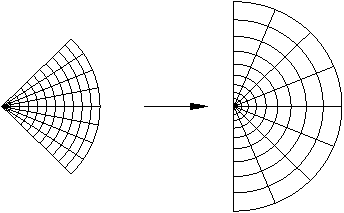
\includegraphics{figures/zsqplot}
\caption{Pengaruh $z^2$ terhadap sektor
$\frac{-\pi}{4} \leq \Arg z \leq \frac{\pi}{4}$, $\sabs{z} <
1.1$.\label{fig:zsqplot}}
\end{myfig}

Hal penting lainnya mengenai fungsi $z \mapsto z^n$ adalah bahwa fungsi ini bersifat $n$-ke-$1$.
Artinya, terdapat $n$ akar pangkat $n$ yang berbeda dari setiap bilangan kompleks
kecuali $0$,
yang dalam suatu pengertian juga memiliki $n$ akar, tetapi semuanya adalah $0$.  Untuk bilangan taknol
$w$, tuliskan $w = re^{i\theta}$.  Mudah diverifikasi bahwa
$n$ akar pangkat $n$ dari $w$ adalah
(dengan menggunakan bentuk polar)
\begin{equation*}
r^{1/n} e^{i\theta/n}
, \quad
r^{1/n} e^{i\theta/n + 2\pi i /n}
, \quad \ldots, \quad
r^{1/n} e^{i\theta/n + 2\pi i (n-1)/n} .
\end{equation*}
Itulah $n$ nilai $z$ berbeda yang memenuhi $z^n=w$.  Nilai-nilai tersebut tersebar
merata pada lingkaran berjari-jari $r^{1/n}$; lihat
\figureref{fig:roots}.  Akar-akar dari $w=1$ disebut
\emph{\myindex{akar satuan}}.

\begin{myfig}
\subimport*{figures/}{roots.pdf_t}
\caption{Delapan akar pangkat $8$ dari suatu bilangan positif $r$:
$r^{1/8}$, $r^{1/8} e^{i \pi / 4}$,  $r^{1/8} e^{i \pi / 2}$,
dan seterusnya.\label{fig:roots}}
\end{myfig}

\begin{exbox}
\begin{exercise}
Buktikan bahwa
\begin{exparts}
\item
Jika $\sabs{z}<1$, maka $\lim\limits_{n\to \infty} z^n = 0$.
\item
Jika $\sabs{z}>1$, maka $\lim\limits_{n\to \infty} z^n = \infty$.
\item
Jika $z \neq 1$ memenuhi $\sabs{z}=1$, maka $z^n$ divergen ketika $n \to
\infty$.
\end{exparts}
\end{exercise}

\begin{exercise}[Mudah]
Pada lingkaran satuan yang diparameterkan oleh sudut $\theta$,
tuliskan $\sin(n\theta)$ dan $\cos(n\theta)$ sebagai kombinasi linear
dari pangkat-pangkat (termasuk pangkat negatif) $z = e^{i\theta}$.
\end{exercise}
\end{exbox}

\subsection{Deret pangkat dan jari-jari konvergensi}

Suatu \emph{\myindex{deret pangkat}} di sekitar $p \in \C$ hanyalah deret
\glsadd{not:powerser}%
\begin{equation*}
\sum_{n=0}^\infty c_n {(z-p)}^n ,
\end{equation*}
dengan $c_n$ berupa bilangan-bilangan kompleks.  Di tempat deret itu konvergen, deret tersebut mendefinisikan
suatu fungsi dari $z$.  Karena deret itu jelas konvergen pada $z=p$, yang perlu diperhatikan adalah
konvergensi di titik-titik lain.  Kita mengatakan deret tersebut
\emph{konvergen}\index{deret pangkat konvergen} jika deret itu konvergen pada
suatu $z \neq p$.

Deret yang paling penting, dan dalam suatu pengertian satu-satunya yang sungguh-sungguh
kita ketahui cara menjumlahkannya, ialah \emph{\myindex{deret geometri}}.

\begin{prop}[Deret geometri]\label{prop:geomseries}
\leavevmode
\begin{enumerate}[(i)]
\item Untuk $z \in \D$,
\begin{equation*}
\frac{1}{1-z} = \sum_{n=0}^\infty z^n .
\end{equation*}
\item Untuk $z \notin \D$,
\begin{equation*}
\sum_{n=0}^\infty z^n \quad \text{divergen.}
\end{equation*}
\item
Diberikan $0 < r < 1$, maka untuk semua $z \in \overline{\Delta_r(0)}$
(yaitu, $\sabs{z} \leq r$)
\begin{equation*}
\abs{\frac{1}{1-z} - \sum_{n=0}^m z^n}
\leq \frac{r^{m+1}}{1-r} .
\end{equation*}
Akibatnya,
karena $\frac{r^{m+1}}{1-r} \to 0$,
deret geometri tersebut konvergen seragam
pada $\overline{\Delta_r(0)}$.
\end{enumerate}
\end{prop}

\begin{proof}
Ketiga butir tersebut mengikuti (rincian diserahkan sebagai latihan) dari
\begin{equation*}
1+z+z^2+\cdots+z^m = \frac{1-z^{m+1}}{1-z} ,
\end{equation*}
untuk semua $z \neq 1$, yang diperoleh dengan mengembangkan
$(1-z)(1+z+z^2+\cdots+z^m)$.
\end{proof}

\begin{exbox}
\begin{exercise}
Lengkapilah rincian bukti \propref{prop:geomseries}.  Jangan melupakan
batas cakram.
\end{exercise}
\end{exbox}

Suatu deret pangkat \emph{konvergen absolut}%
\index{konvergen absolut!deret pangkat}%
\index{konvergensi absolut!deret pangkat}
jika deret berikut konvergen:
\begin{equation*}
\sum_{n=0}^\infty \sabs{c_n} \sabs{z-p}^n .
\end{equation*}
Untuk $N < M$,
\begin{equation*}
\abs{\sum_{n=N+1}^M c_n {(z-p)}^n}
\leq
\sum_{n=N+1}^M \sabs{c_n} \sabs{z-p}^n.
\end{equation*}
Jadi, jika barisan jumlah parsial
$\sum \sabs{c_n} \sabs{z-p}^n$ merupakan barisan Cauchy, demikian pula barisan
jumlah parsial $\sum c_n {(z-p)}^n$.  Dengan demikian,
deret yang konvergen absolut
memang konvergen.

Misalkan $r = \sabs{z-p}$, dan tinjau deret real $\sum \sabs{c_n} r^n$.  Definisikan
\begin{equation} \label{eq:rconvdef}
R = \frac{1}{\limsup\limits_{n \to \infty} \sqrt[n]{\sabs{c_n}}} ,
\end{equation}
dengan menafsirkan $\nicefrac{1}{\infty} = 0$ dan $\nicefrac{1}{0} = \infty$,
sehingga $R=\infty$ diperbolehkan.\footnote{%
Kita tidak menggunakan \myquote{pengertian bilangan real diperluas} di sini;
kita sebenarnya hanya memperluas bilangan real taknegatif, sehingga
sesuatu seperti $\nicefrac{1}{0}=\infty$ masuk akal, dengan alasan yang sama
seperti pada bola Riemann.}
Menurut uji akar standar, deret $\sum \sabs{c_n} r^n$
konvergen jika
\begin{equation*}
\limsup_{n \to \infty} \sqrt[n]{\sabs{c_n} r^n} = 
r \limsup_{n \to \infty} \sqrt[n]{\sabs{c_n}} = r \frac{1}{R} < 1 .
\end{equation*}
Jadi deret pangkat tersebut konvergen absolut ketika $r < R$.
Jika $r \frac{1}{R} > 1$, maka untuk tak berhingga banyaknya $n$,
$\sabs{c_n {(z-p)}^n} > 1$. Jadi deret tersebut
divergen jika $r > R$.
%$\sum c_n {(z-p)}^n$ divergen.
Lihat \figureref{fig:radiusconvcomplex}.
Kita telah membuktikan:

\begin{prop}[Teorema Cauchy--Hadamard\footnote{%
Cauchy menerbitkan hasil ini pada tahun 1821, dan Hadamard, meskipun juga berasal dari
Prancis, tidak mengetahuinya dan menerbitkannya dalam disertasinya pada tahun 1888.}]
\index{teorema Cauchy--Hadamard}
Suatu deret pangkat $\sum c_n {(z-p)}^n$ konvergen absolut jika
$\sabs{z-p} < R$ dan divergen jika
$\sabs{z-p} > R$, dengan $R$ didefinisikan oleh \eqref{eq:rconvdef}.
\end{prop}

\begin{myfig}
\subimport*{figures/}{radiusconvcomplex.pdf_t}
\caption{Jari-jari konvergensi.\label{fig:radiusconvcomplex}}
\end{myfig}

Bilangan $R$ disebut \emph{\myindex{jari-jari konvergensi}}.
Deret pangkat tersebut konvergen absolut
di dalam cakram $\Delta_R(p)$, dan divergen
di komplemen dari penutupan $\overline{\Delta_R(p)}$.
Konvergensi (atau divergensi) pada lingkaran batas $\partial \Delta_R(p)$
merupakan persoalan yang rumit.

Suatu kriteria yang berguna untuk konvergensi ialah bahwa barisan
$\bigl\{ \sabs{c_n} r^n \bigr\}$
terbatas setiap kali $0 < r < R$.

\begin{prop} \label{prop:cnrnbounded}
Deret $\sum c_n {(z-p)}^n$ konvergen di $\Delta_{R}(p)$ untuk suatu
$R > 0$ jika dan hanya jika
untuk setiap $r$ dengan
$0 < r < R$, terdapat $M > 0$ sedemikian sehingga
\begin{equation*}
\sabs{c_n} \leq \frac{M}{r^n} \qquad \text{untuk semua } n .
\end{equation*}
\end{prop}

Tidak selalu benar bahwa $\bigl\{ \sabs{c_n} R^n \bigr\}$
terbatas jika $R$ adalah jari-jari konvergensi.
Kedua deret $\sum z^n$ dan $\sum n z^n$ sama-sama memiliki
jari-jari konvergensi $1$, sedangkan barisan koefisien
terbatas pada kasus pertama dan
tidak terbatas pada kasus kedua.  Namun, $\{ n r^n \}$ terbatas untuk setiap $r < 1$.

\begin{proof}
Andaikan deret tersebut konvergen di $\Delta_{R}(p)$ dan
$0 < r < R$.  Maka (menurut Cauchy--Hadamard) $\sum \sabs{c_n}r^n$ konvergen,
dan suku-suku deret tersebut terbatas.

Sebaliknya, tetapkan $r$ dengan $0 < r < R$, andaikan
$\sabs{c_n} r^n \leq M$ untuk semua $n$, dan andaikan $0 < s < r$.
Maka
\begin{equation*}
\sqrt[n]{\sabs{c_n} s^n}=
\frac{s}{r}\sqrt[n]{\sabs{c_n} r^n} \leq \frac{s}{r} \sqrt[n]{M} .
\end{equation*}
Limsup ruas kanan lebih kecil secara ketat daripada $1$
karena $\nicefrac{s}{r} < 1$.
Jadi, dengan uji akar sekali lagi, deret tersebut konvergen absolut di
$\overline{\Delta_s(p)}$.
Karena $s$ dan $r$ dengan $0 < s < r < R$ sebarang,
deret tersebut konvergen (absolut) di $\Delta_R(p)$.
\end{proof}

Bukti tersebut cukup lazim bagi hasil konvergensi deret pangkat.
Konvergensi di $\Delta_R(p)$ berarti keterbatasan
$\{ \sabs{c_n} r^n \}$ untuk $\Delta_r(p)$ yang lebih kecil, yang hanya memberi kita konvergensi
di $\Delta_s(p)$.  Lihat \figureref{fig:threediscs}.  Namun, karena $s$ dan $r$
sebarang, kita memperoleh konvergensi di~$\Delta_R(p)$.
\begin{myfig}
\subimport*{figures/}{threediscs.pdf_t}
\caption{Ketiga cakram dalam bukti konvergensi.\label{fig:threediscs}}
\end{myfig}

\begin{exbox}
\begin{exercise}
Buktikan ketaksamaan segitiga untuk deret.  Jika $\sum_{n=0}^\infty c_n$
konvergen, maka $\abs{\sum_{n=0}^\infty c_n} \leq \sum_{n=0}^\infty
\sabs{c_n}$ (ruas kanan mungkin bernilai $\infty$).
\end{exercise}
\end{exbox}

Konvergensi di dalam jari-jari konvergensi bahkan lebih baik daripada sekadar konvergensi absolut.
Misalkan $K \subset \C$ suatu himpunan.
Suatu deret pangkat $\sum c_n {(z-p)}^n$
\emph{konvergen absolut seragam}%
\index{konvergen absolut seragam!deret pangkat}%
\index{konvergensi absolut seragam!deret pangkat}
untuk $z \in K$ apabila $\sum \sabs{c_n} \sabs{z-p}^n$
konvergen seragam untuk $z \in K$.
Andaikan suatu deret konvergen absolut seragam pada $K$.  Deret itu konvergen absolut,
jadi deret itu konvergen, dan
\begin{equation*}
\abs{
\sum_{n=0}^\infty c_n {(z-p)}^n
-
\sum_{n=0}^{m} c_n {(z-p)}^n
}
=
\abs{\sum_{n=m+1}^\infty c_n {(z-p)}^n} \leq
\sum_{n=m+1}^\infty \sabs{c_n} \sabs{z-p}^n .
\end{equation*}
Ruas kanan menuju nol secara seragam terhadap $z \in K$ ketika $m \to \infty$,
dan oleh karena itu
deret yang konvergen absolut seragam juga konvergen
seragam.  Jadi namanya sesuai dengan sifatnya.

\begin{prop}
Misalkan $\sum c_n {(z-p)}^n$ suatu deret pangkat dengan jari-jari konvergensi $R
> 0$.  Jika $0 < r < R$, maka deret pangkat tersebut konvergen absolut seragam
pada $\overline{\Delta_r(p)}$. Selanjutnya, misalkan $U = \Delta_R(p)$ jika $R < \infty$ dan
$U = \C$ jika $R=\infty$, dan misalkan $K \subset U$ kompak.
Maka deret tersebut konvergen absolut seragam pada $K$.
\end{prop}

Secara kurang formal, suatu deret pangkat konvergen seragam (absolut) pada
subhimpunan kompak dari domain konvergensinya.

\begin{proof}
Tanpa mengurangi keumuman, andaikan $R < \infty$.
Andaikan $0 < r < R$.  Karena $\sum c_n {(z-p)}^n$ konvergen absolut
pada $\Delta_R(p)$, deret
$\sum \sabs{c_n} r^n$ konvergen (dan khususnya setiap ekor
deret tersebut konvergen).  Jadi untuk $z \in \overline{\Delta_r(p)}$,
\begin{equation*}
\abs{
\sum_{n=0}^\infty \sabs{c_n} \sabs{z-p}^n
-
\sum_{n=0}^{m} \sabs{c_n} \sabs{z-p}^n
}
\leq
\sum_{n=m+1}^\infty \sabs{c_n} r^n .
\end{equation*}
Ruas kanan, yang tidak bergantung pada $z$,
menuju nol ketika $m \to \infty$, sehingga
deret $\sum \sabs{c_n} \sabs{z-p}^n$ konvergen seragam
pada $\overline{\Delta_r(p)}$.

Jika $K \subset \Delta_{R}(p)$ kompak, maka terdapat suatu $r <
R$ sedemikian sehingga $K \subset \Delta_r(p)$ (tinjau suatu selimut terbuka
dari $K$ oleh cakram-cakram $\Delta_r(p)$ untuk semua $r < R$).  Hasilnya mengikuti.
\end{proof}

\begin{exbox}
\begin{exercise}
Tunjukkan bahwa deret $\sum_{n=1}^\infty \frac{1}{n^2} z^{n}$ memiliki jari-jari
konvergensi $1$, dan
tunjukkan bahwa deret itu konvergen absolut pada batas cakram satuan.  Oleh karena itu,
deret itu sesungguhnya konvergen seragam pada seluruh cakram satuan tertutup.
\end{exercise}

\begin{exercise}
Tunjukkan bahwa
$\sum_{n=0}^\infty n^n z^{n^n}$ memiliki jari-jari konvergensi $1$,
sedangkan
$\sum_{n=0}^\infty n^n z^{n}$ tidak konvergen
untuk setiap $z \neq 0$.
\end{exercise}

\begin{exercise}
Andaikan
$\sum_{n=0}^\infty c_n z^{n}$ konvergen pada $z=1$, tetapi tidak konvergen absolut.
Buktikan bahwa jari-jari konvergensinya adalah $1$.
\end{exercise}

\begin{exercise}[Uji-$M$ Weierstrass]
\label{exercise:weierMtest}
Misalkan $X$ suatu himpunan dan andaikan $f_n \colon X \to \C$ adalah
barisan fungsi sedemikian sehingga
$\abs{f_n(x)} \leq M_n$ untuk semua $x \in X$ dan $n \in \N$.  Jika $\sum M_n <
\infty$, maka $\sum f_n(x)$ konvergen absolut seragam pada $X$
($\sum \sabs{f_n(x)}$ konvergen seragam pada $X$).
\end{exercise}

\begin{exercise}
Andaikan
$\sum_{n=0}^\infty a_n z^{n}$ dan $\sum_{n=0}^\infty b_n z^{n}$
memiliki jari-jari konvergensi setidaknya $r > 0$.  Tunjukkan bahwa
deret jumlah
$\sum_{n=0}^\infty (a_n+b_n) z^{n}$ memiliki jari-jari konvergensi setidaknya
$r$ dan konvergen menuju jumlah kedua deret tersebut.
\end{exercise}

\begin{exercise}
Diberikan $R > 1$, carilah dua deret pangkat
$\sum_{n=0}^\infty a_n z^{n}$ dan $\sum_{n=0}^\infty b_n z^{n}$,
sedemikian sehingga keduanya memiliki jari-jari konvergensi tepat $1$, tetapi
jumlahnya
$\sum_{n=0}^\infty (a_n+b_n) z^{n}$ memiliki jari-jari konvergensi
tepat $R$.  Petunjuk: Mula-mula tentukan deret dengan jari-jari konvergensi
tepat $R$.
\end{exercise}

\begin{exercise}
Andaikan
$\sum_{n=0}^\infty a_n z^{n}$ dan $\sum_{n=0}^\infty b_n z^{n}$
memiliki jari-jari konvergensi setidaknya $r > 0$.  Misalkan
$c_n = \sum_{k=0}^n a_{n-k}b_k$.  Tunjukkan bahwa
deret
$\sum_{n=0}^\infty c_n z^{n}$ memiliki jari-jari konvergensi setidaknya
$r$ dan konvergen menuju hasil kali kedua deret tersebut.
Petunjuk: Kuncinya adalah meninjau suatu titik tempat kedua deret konvergen absolut,
lalu menggunakan konvergensi absolut tersebut.
\end{exercise}

\begin{exercise}
Jika $\sum_{n=0}^\infty a_n z^{n}$ dan $\sum_{n=0}^\infty b_n z^{n}$
konvergen dan sama di suatu cakram $\Delta_r(0)$, maka $a_n = b_n$
untuk semua $n$.  Petunjuk: Mula-mula andaikan $b_n = 0$ untuk semua $n$
dan carilah $n$ pertama yang memenuhi $a_n \neq 0$.
\end{exercise}
\end{exbox}

\begin{remark}
Beberapa latihan terakhir menyatakan bahwa kita dapat menjumlahkan dan mengalikan deret pangkat.
Penjumlahan deret pangkat bersifat langsung, dan akan segera kita perlukan.
Perkalian akan jauh lebih mudah nanti, setelah
kita menunjukkan bahwa deret pangkat bersifat
holomorfik dan sebaliknya, tetapi Anda tetap sebaiknya mencoba latihan itu sekarang karena latihan tersebut
merupakan praktik yang baik.
\end{remark}

%%%%%%%%%%%%%%%%%%%%%%%%%%%%%%%%%%%%%%%%%%%%%%%%%%%%%%%%%%%%%%%%%%%%%%%%%%%%%%

\section{Fungsi analitik}
\label{sec:analfuncs}

\subsection{Definisi}

Fungsi yang memiliki deret pangkat konvergen disebut analitik.
Sejak awal kalkulus hingga abad ke-19,
ketika matematikawan mempertimbangkan suatu \myquote{fungsi,} yang sebenarnya mereka maksud ialah
\myquote{fungsi analitik} (atau sesuatu yang serupa) dalam bahasa modern.
Kita membahas
fungsi analitik-kompleks maupun analitik-real bergantung pada apakah
variabelnya real atau kompleks, dan fungsi-fungsi itu dapat bergantung pada satu atau beberapa variabel.
Kita tertarik pada fungsi analitik-kompleks satu variabel.
Karena kemungkinan timbulnya kebingungan kecil, kita cukup mengatakan \myquote{analitik} alih-alih
\myquote{analitik-kompleks.}

\begin{defn}
Misalkan $U \subset \C$ terbuka.  Suatu fungsi $f \colon U \to \C$
disebut \emph{\myindex{analitik}}\index{analitik-kompleks}
jika untuk setiap $p \in U$, terdapat
$r > 0$ dan suatu
deret pangkat $\sum c_n {(z-p)}^n$ yang konvergen menuju $f$ pada $\Delta_r(p) \subset
U$.
\end{defn}

\begin{exbox}
\begin{exercise}[Mudah]
Buktikan bahwa polinomial $P(z)$ bersifat analitik.
\end{exercise}

\begin{exercise}
Buktikan bahwa $\nicefrac{1}{z}$ bersifat analitik di $\C \setminus \{ 0 \}$
dengan menuliskan secara eksplisit
suatu deret pangkat di setiap $p \in \C \setminus \{ 0 \}$
menggunakan deret geometri.
\end{exercise}

\begin{exercise}
Andaikan $f(z) = \sum_{n=0}^\infty a_n z^n$ konvergen dan mendefinisikan suatu
fungsi pada $\D$ sedemikian sehingga $f(z) = f(-z)$ untuk semua $z \in \D$ ($f$
\myquote{genap}).
Buktikan bahwa terdapat suatu fungsi yang didefinisikan oleh deret pangkat
$g(z) = \sum_{n=0}^\infty b_n z^n$ yang konvergen di $\D$ sedemikian sehingga
$f(z) = g(z^2)$.
\end{exercise}
\end{exbox}

\subsection{Fungsi analitik bersifat holomorfik}

Pada akhirnya, kita akan melihat bahwa fungsi analitik dan fungsi holomorfik
adalah hal yang sama.\footnote{%
Karena alasan ini, beberapa penulis mendefinisikan \myquote{analitik} sebagai terdiferensialkan secara kompleks,
yang pada akhirnya tidak menimbulkan masalah, tetapi saat ini akan menimbulkannya.}
Kita mulai dengan membuktikan bahwa
fungsi analitik bersifat holomorfik, yakni terdiferensialkan secara
kompleks.

\begin{prop}
\pagebreak[2]
Misalkan $f \colon \Delta_R(p) \to \C$ didefinisikan oleh
\begin{equation*}
f(z) = \sum_{n=0}^\infty c_n {(z-p)}^n ,
\qquad \text{yang konvergen di } \Delta_R(p) .
\end{equation*}
Maka $f$ terdiferensialkan secara kompleks di setiap $z \in \Delta_R(p)$, dan
\begin{equation*}
f'(z) = \sum_{n=1}^\infty n c_n {(z-p)}^{n-1} ,
\qquad \text{yang konvergen di } \Delta_R(p) .
\end{equation*}
\end{prop}

\begin{proof}
Tanpa mengurangi keumuman, misalkan $p=0$.
Diferensialkan $z^n$ pada suatu $z_0$ dengan meninjau hasil bagi
selisih
\begin{equation*}
\frac{z^n-z_0^n}{z-z_0}
=
\sum_{k=0}^{n-1}
z^k z_0^{n-1-k} ,
\end{equation*}
yang menuju $n z_0^{n-1}$ ketika $z \to z_0$, karena
ruas kanan terdefinisi bahkan jika $z = z_0$.
Terapkan rumus tersebut pada $f$
suku demi suku.  Untuk $z_0,z \in \Delta_R(0)$,
\begin{equation*}
\frac{f(z) - f(z_0)}{z-z_0}
=
\sum_{n=1}^\infty c_n \frac{z^n-z_0^n}{z-z_0}
=
\sum_{n=1}^\infty c_n \sum_{k=0}^{n-1} z^k z_0^{n-1-k} .
\end{equation*}
Kita harus menunjukkan bahwa ekspresi di ruas kanan memberikan suatu fungsi kontinu dari $z$
pada $z_0$.
Fungsi itu kontinu pada $z_0$ asalkan deret
dalam ekspresi tersebut konvergen seragam untuk $z$ di suatu
lingkungan $z_0$.

Susunannya akan sama seperti pada \figureref{fig:threediscs}.
Misalkan $r$ dan $s$ memenuhi $0 < s < r < R$ dan andaikan $z_0$ serta $z$ berada
di $\Delta_s(0)$.
\begin{equation*}
\abs{c_n \sum_{k=0}^{n-1} z^k z_0^{n-1-k}}
\leq
\sum_{k=0}^{n-1} 
\sabs{c_n}
s^{n-1}
=
n
\sabs{c_n} s^{n-1}
=
n
\sabs{c_n} r^{n-1} {\left(\frac{s}{r}\right)}^{n-1} .
\end{equation*}
Ekspresi
$\sabs{c_n} r^{n-1}$ dibatasi oleh suatu $M > 0$ untuk semua $n$,
karena deret untuk $f$ konvergen
di $\Delta_R(0)$ dan $r < R$.
Karena
\begin{equation*}
\sqrt[n]{
n \sabs{c_n} s^{n-1}
}
=
\sqrt[n]{
n \sabs{c_n} r^{n-1} {\left(\frac{s}{r}\right)}^{n-1}
}
\leq
\sqrt[n]{
n M {\left(\frac{s}{r}\right)}^{n-1}
}
\quad\underset{\text{ketika } n \to \infty}{\to}\quad
\frac{s}{r} < 1 ,
\end{equation*}
uji akar menunjukkan bahwa
$\sum n \sabs{c_n} s^{n-1}$
konvergen.
Jadi deret untuk hasil bagi selisih,
\begin{equation*}
\sum_{n=1}^\infty c_n \sum_{k=0}^{n-1} z^k z_0^{n-1-k} ,
\end{equation*}
konvergen seragam dalam $z$ pada $\Delta_s(0)$, dan
kita dapat menukar limit $z \to z_0$ dengan limit deret:
\begin{equation*}
\lim_{z \to z_0}
\frac{f(z)-f(z_0)}{z-z_0}
=
\sum_{n=1}^\infty c_n \sum_{k=0}^{n-1} z_0^k z_0^{n-1-k}
=
\sum_{n=1}^\infty n c_n z_0^{n-1} .
\end{equation*}
Karena $s$ dan $r$ sebarang, konvergensi berlaku di seluruh
$\Delta_R(0)$.
\end{proof}

Jadi turunan suatu deret pangkat kembali diberikan oleh deret pangkat.
Dengan induksi, diperoleh bahwa suatu deret pangkat terdiferensialkan secara kompleks
tak berhingga kali.

\begin{cor} \label{cor:convpowserinfdif}
\pagebreak[2]
Misalkan $f \colon \Delta_R(p) \to \C$ didefinisikan oleh
\begin{equation*}
f(z) = \sum_{n=0}^\infty c_n {(z-p)}^n ,
\qquad \text{yang konvergen di } \Delta_R(p) .
\end{equation*}
Maka $f$ terdiferensialkan secara kompleks tak berhingga kali di $\Delta_R(p)$,
dan turunan ke-$k$ diberikan oleh
\begin{equation*}
f^{(k)}(z) = \sum_{n=k}^\infty n(n-1)\cdots(n-k+1) c_n {(z-p)}^{n-k} ,
\qquad \text{yang konvergen di } \Delta_R(p) .
\end{equation*}
Selanjutnya,
\begin{equation*}
c_n =
\frac{f^{(n)}(p)}{n!} .
\end{equation*}
\end{cor}

\begin{exbox}
\begin{exercise}
Lengkapilah rincian bukti korolari tersebut.
\end{exercise}
\end{exbox}

Salah satu akibat korolari ini yang perlu
ditekankan ialah bahwa jika $f$ diberikan oleh deret pangkat konvergen di
$\Delta_R(p)$ seperti di atas, maka deret pangkat tersebut tunggal.
Kita telah melihat kesimpulan ini dalam latihan sebelumnya.
Di sini kesimpulan tersebut
mengikuti dari rumus untuk koefisien $c_n$.  Bahkan,
koefisien hanya bergantung pada nilai-nilai $f$ dalam suatu lingkungan
$p$ yang kecilnya sebarang.

Jika kita menerapkan korolari tersebut pada fungsi analitik di setiap titik,
kita menemukan bahwa fungsi-fungsi itu terdiferensialkan tak berhingga kali:

\begin{cor} \label{cor:analinfdif}
Suatu fungsi analitik terdiferensialkan secara kompleks tak berhingga kali dan setiap
turunannya bersifat analitik.
\end{cor}

\begin{remark}
Satu persoalan halus ialah bahwa walaupun kita membuktikan fungsi analitik
terdiferensialkan secara kompleks karena memiliki representasi deret pangkat,
kita belum membuktikan bahwa suatu deret pangkat konvergen mendefinisikan fungsi
analitik.  Yang tersisa ialah membuktikan bahwa deret pangkat yang konvergen
di $\Delta_R(p)$ dapat
dikembangkan di sekitar titik lain dalam $\Delta_R(p)$.  Hal itu akan mengikuti
setelah kita membuktikan bahwa fungsi holomorfik bersifat analitik.
\end{remark}

\begin{exbox}
\begin{exercise}
Andaikan $f \colon \Delta_R(0) \to \C$ diberikan oleh deret pangkat
konvergen
$f(z) = \sum_{n=0}^\infty c_n z^n$.
Andaikan untuk suatu $\epsilon > 0$, $f(x) = 0$ bagi semua $x \in
(-\epsilon,\epsilon)$ (suatu interval pada garis real).
Dengan menggunakan korolari tersebut,
buktikan bahwa $c_n = 0$ untuk semua $n$ dan karena itu $f$ identik nol.
\end{exercise}

\begin{exercise} \label{exercise:antidefpowerser}
Andaikan $f \colon \Delta_R(p) \to \C$ diberikan oleh deret pangkat
konvergen
$f(z) = \sum_{n=0}^\infty c_n {(z-p)}^n$.
Lakukan antidiferensiasi:
Tunjukkan bahwa terdapat suatu deret pangkat yang konvergen di $\Delta_R(p)$
dan turunan kompleksnya adalah $f(z)$.
\end{exercise}

\begin{exercise} 
Andaikan $f \colon \Delta_R(0) \to \C$ diberikan oleh deret pangkat
konvergen
$f(z) = \sum_{n=0}^\infty c_n {z}^n$ dan $R > 1$.
Tunjukkan bahwa terdapat $M>0$ sedemikian sehingga
$\sabs{f^{(n)}(0)} \leq n! M$ untuk semua $n$.
\end{exercise}
\end{exbox}

\subsection{Fungsi eksponensial}

Kita telah menjumpai fungsi eksponensial kompleks $e^z$ sebelumnya
(\subsectionref{subsection:firstdefexp}), dan kita telah membuktikan
bahwa fungsi tersebut holomorfik dan merupakan turunannya sendiri
(\exerciseref{exercise:exponentialholomorphic}).  Sekarang kita dapat melihat fakta ini
dari sudut pandang berbeda.\footnote{%
Sudut pandang itu sama dengan tempat kelam dalam masa lalu Anda,
yaitu kuliah persamaan diferensial tingkat sarjana ketika Anda mempelajari
metode deret pangkat untuk menyelesaikan ODE.}
Kita menyatakan bahwa kita sebenarnya dapat mendefinisikan fungsi eksponensial
menggunakan deret pangkat.

\begin{prop}
Deret pangkat
\begin{equation*}
f(z) = \sum_{n=0}^\infty \frac{1}{n!} z^n ,
\end{equation*}
adalah deret pangkat konvergen tunggal di titik asal
sedemikian sehingga $f(0)=1$ dan $f'=f$.
Selain itu, deret tersebut konvergen pada $\C$ dan
$f(z) = e^z$.
\end{prop}

\begin{proof}
Sekarang kita mengetahui bahwa deret pangkat bersifat holomorfik dan mengetahui cara
mendiferensialkannya: Kita melakukannya suku demi suku, yakni, \myquote{secara formal.}
Andaikan kita memiliki deret pangkat yang konvergen di titik asal
\begin{equation*}
f(z) = \sum_{n=0}^\infty c_n z^n
\end{equation*}
sedemikian sehingga $f(0)=1$ dan $f'=f$.
Jelas, $f(0)=1$ mengakibatkan $c_0 = 1$.
Caranya ialah menentukan bagian deret yang lain.
Jadi,
\begin{equation*}
f'(z) =
\sum_{n=1}^\infty n c_n z^{n-1} =
\sum_{n=0}^\infty (n+1) c_{n+1} z^{n} .
\end{equation*}
Karena koefisien deret pangkat di nol tunggal, kita memperoleh
$c_n = (n+1) c_{n+1}$.  Dengan induksi, $c_n = \frac{1}{n!}$.
Tidak sulit untuk memeriksa secara langsung (latihan)
bahwa deret tersebut konvergen di seluruh $\C$.

Mari kita buktikan bahwa $f$ adalah fungsi eksponensial.  Kedua fungsi
holomorfik, fungsi eksponensial tidak pernah nol, dan keduanya sama dengan
turunannya masing-masing.  Jadi,
\begin{equation*}
\frac{d}{dz} \left[ \frac{f(z)}{\exp(z)} \right]
=
\frac{f'(z)\exp(z) - f(z) \exp'(z)}{{\bigl(\exp(z)\bigr)}^2}
=
\frac{f(z)\exp(z) - f(z) \exp(z)}{{\bigl(\exp(z)\bigr)}^2}
= 0.
\end{equation*}
Dengan demikian, $f(z) = C \exp(z)$ untuk suatu konstanta (\propref{prop:zeroder}).
Karena $f(0) = \exp(0) = 1$,
kita simpulkan $C=1$.
\end{proof}

\begin{exbox}
\begin{exercise}
Buktikan bahwa deret untuk fungsi eksponensial konvergen dengan menghitung
jari-jari konvergensinya secara langsung
(misalnya, tunjukkan bahwa deret tersebut konvergen untuk setiap $z \in \C$).
\end{exercise}

\begin{exercise}
Hitung deret untuk $\sin z$ dan $\cos z$, lalu tunjukkan bahwa fungsi-fungsi ini memenuhi
$f''(z) = -f(z)$.
\end{exercise}

\begin{exercise}
Tunjukkan bahwa terdapat fungsi holomorfik $f \colon \C \to \C$ yang
memenuhi $f'(z) + z f(z) = 0$ dan $f(0) = 1$.  Petunjuk: Selesaikan secara formal
sebagai deret pangkat,
lalu lihat apakah Anda dapat menebak jawabannya dalam \myquote{bentuk tertutup,} yakni dalam
bentuk fungsi eksponensial.  Petunjuk \#2: Berapakah $f'(0)$?
\end{exercise}

\begin{exercise}
Diberikan $a,b \in \C$, tunjukkan bahwa terdapat fungsi holomorfik $f \colon \C \to
\C$ sedemikian sehingga $f''(z) = z f(z)$, serta $f(0) = a$ dan $f'(0) = b$.
Petunjuk: Definisikan secara formal dan tunjukkan konvergensinya.
Catatan: Ini adalah \emph{\myindex{fungsi Airy}}, dan fungsi-fungsi tersebut memiliki sejumlah
perilaku menarik.  Pada garis real fungsi-fungsi itu berosilasi seperti sinus dan kosinus
untuk $z$ negatif dan berperilaku seperti fungsi eksponensial untuk $z$ positif.
\end{exercise}
\end{exbox}

\subsection{Teorema identitas}

Salah satu sifat utama fungsi analitik ialah bahwa setelah kita mengetahuinya
di suatu lingkungan, kita mengetahuinya di mana-mana.  Bahkan, berlaku pernyataan yang jauh lebih
umum; kita hanya perlu mengetahui suatu fungsi analitik pada himpunan yang memiliki
titik limit.

\begin{thm}[Identitas]\index{teorema identitas!fungsi holomorfik}%
\label{thm:identity}
Andaikan $U \subset \C$ suatu domain,
dan $f \colon U \to \C$ analitik.
Jika $Z_f = \bigl\{ z \in U : f(z) = 0 \bigr\}$
memiliki titik limit di $U$, maka $f$ identik nol.
Dengan kata lain, semua titik $Z_f$ terisolasi kecuali jika $f \equiv 0$.
\end{thm}

\begin{defn}
Titik-titik dalam himpunan $Z_f$ disebut \emph{titik nol}\index{titik nol} dari $f$.
\end{defn}

Bagian \myquote{Dengan kata lain} merupakan
salah satu akibat teorema ini yang akan sering kita gunakan.  Secara lebih
konkret, jika $f(p)=0$, tetapi $f$ tidak
identik nol, maka terdapat cakram $\Delta_r(p)$ sedemikian sehingga
$f(z) \neq 0$ untuk semua $z \in \Delta_r(p) \setminus \{ 0 \}$.

Penerapan umum lain dari teorema tersebut ialah pernyataan yang lebih lemah berikut:
\myquote{Jika fungsi itu nol pada suatu subhimpunan terbuka takkosong, maka $f \equiv 0$.}
Renungkan implikasinya: Jika $f \colon U \to \C$ analitik, dan kita mengetahui
$f$ pada cakram kecil $\Delta_r(p)$ untuk $r$ sekecil apa pun, maka
kita mengetahui $f$ di seluruh $U$.

\begin{proof}
Andaikan $f$ tidak identik nol.
Himpunan $Z_f$ tertutup (tentu saja di $U$) karena $f$ kontinu.  Kita harus menunjukkan
bahwa titik-titik $Z_f$ terisolasi.
Tanpa mengurangi keumuman, andaikan $0 \in U$ dan $0 \in Z_f$,
serta andaikan $0$ tidak berada di interior $Z_f$.
Di dekat $0$, tuliskan
\begin{equation*}
f(z) = \sum_{n=0}^\infty c_n z^n .
\end{equation*}
Karena $f(0) = 0$, $c_0 =0$.  Misalkan $k$ adalah nilai $k$ terkecil yang memenuhi $c_k \neq 0$;
$k$ ini ada karena jika tidak, $f$ akan identik nol di dekat $0$
dan kita mengandaikan $0$ tidak berada di interior $Z_f$.  Maka
\begin{equation*}
f(z) = z^k \sum_{n=k}^\infty c_n z^{n-k} = z^k g(z) .
\end{equation*}
Deret $g(z)$ adalah deret pangkat konvergen dan
$g(0) = c_k \neq 0$.
Suatu deret pangkat kontinu, sehingga $g(z) \neq 0$ di seluruh
lingkungan tertentu dari $0$.
Karena $z^k$ hanya nol pada $0$, kita memperoleh bahwa $0$ adalah titik terisolasi dari $Z_f$.

Jadi satu-satunya titik $Z_f$ yang tidak terisolasi ialah titik-titik yang berada di
interior $Z_f$.  Misalkan $Z_f' \subset Z_f$ adalah himpunan titik takterisolasi
dari $Z_f$.  Himpunan ini harus tertutup karena $Z_f$ tertutup, dan tidak ada barisan
titik di $Z_f'$ yang dapat
memiliki titik terisolasi dari $Z_f$ sebagai limit.
Kita telah membuktikan di atas bahwa titik
takterisolasi harus merupakan titik interior $Z_f$ (dan karenanya juga $Z_f'$).
Jadi $Z_f'$ terbuka sekaligus tertutup.  Karena $U$ terhubung dan
$Z_f' \neq U$, kita simpulkan $Z_f' = \emptyset$.
Dengan demikian semua titik $Z_f$ terisolasi.
\end{proof}

Gagasan berguna dari bukti tersebut yang patut ditekankan
ialah bahwa jika kita memiliki deret pangkat $f(z)$ di $a$,
dan $f$ memiliki titik nol di $a$ (serta tidak identik nol),
kita dapat mengeluarkan faktor suatu pangkat dari $z-a$,
\begin{equation*}
f(z) = {(z-a)}^k g(z) ,
\end{equation*}
dengan $g(z)$ suatu deret pangkat di $a$ sedemikian sehingga $g(a) \neq 0$.

\begin{exbox}
\begin{exercise}
Andaikan $U \subset \C$ suatu domain,
$f \colon U \to \C$ dan $g \colon U \to \C$ analitik,
dan himpunan $\bigl\{ z \in U : f(z) = g(z) \bigr\}$ memiliki titik
limit di $U$.
Buktikan bahwa $f \equiv g$.
\end{exercise}

\begin{exercise}
\begin{exparts}
\item
Andaikan $U \subset \C$ suatu domain,
$f \colon U \to \C$ dan $g \colon U \to \C$ analitik,
dan $f(z)g(z) = 0$ untuk semua $z \in U$.
Buktikan bahwa $f$ atau $g$ identik nol.
(Dengan kata lain, gelanggang fungsi holomorfik pada $U$ adalah suatu daerah
integral.)
\item
Carilah $U$ yang terbuka tetapi tak terhubung serta fungsi holomorfik $f$ dan $g$,
sedemikian sehingga tetap berlaku $fg = 0$, tetapi baik $f$ maupun $g$ tidak identik nol.
\end{exparts}
\end{exercise}

\begin{exercise}
Andaikan $U \subset \C$ suatu domain dan $f \colon U \to \C$
analitik dan tidak konstan.  Tunjukkan bahwa jika $K \subset U$ kompak,
maka $Z_f \cap K$ berhingga.
\end{exercise}

\begin{exercise}
Andaikan $U \subset \C$ suatu domain, $f \colon U \to \C$ dan $g \colon U \to
\C$ analitik, serta $p \in U$.  Andaikan $f^{(k)}(p) = g^{(k)}(p)$
untuk $k=0,1,2,\ldots$.  Buktikan bahwa $f \equiv g$.
\end{exercise}

\begin{exercise}
Andaikan $U \subset \C$ suatu domain dan $f \colon U \to \C$ analitik.
Buktikan bahwa jika $f'(z) = 0$ untuk
semua $z$ dalam suatu lingkungan dari $z_0 \in U$, maka $f$ konstan.
\end{exercise}

\begin{exercise}
Andaikan $U \subset \C$ suatu domain, $a, b, c \in \C$, dan $z_0 \in U$.
Tunjukkan bahwa
solusi analitik $f$ pada $U$ bagi persamaan linear $f'(z) = a f(z) + b$
dengan $f(z_0) = c$ bersifat tunggal.  Petunjuk: Tunjukkan bahwa deret pangkat di $z_0$ ditentukan secara
tunggal.  Cukup tunjukkan ketunggalan, tidak perlu menunjukkan keberadaan.
\end{exercise}
\end{exbox}

Salah satu kekurangan fungsi analitik ialah tidak adanya fungsi analitik dengan
dukungan kompak pada $\C$.  \emph{\myindex{Dukungan}}
suatu fungsi $f \colon U
\to \C$ adalah penutupan (di $U$) dari himpunan
$\bigl\{ z \in U : f(z) \neq 0 \bigr\}$, yakni,
dukungannya adalah $\overline{U \setminus Z_f} \cap U$.

\begin{exbox}
\begin{exercise}
Misalkan $U \subset \C$ suatu domain dan $f \colon U \to \C$ analitik serta
tidak identik nol.
Tunjukkan bahwa dukungan $f$ adalah $U$.
Khususnya, dukungan tersebut tidak dapat kompak.
\end{exercise}
\end{exbox}



%%%%%%%%%%%%%%%%%%%%%%%%%%%%%%%%%%%%%%%%%%%%%%%%%%%%%%%%%%%%%%%%%%%%%%%%%%%%%%
%%%%%%%%%%%%%%%%%%%%%%%%%%%%%%%%%%%%%%%%%%%%%%%%%%%%%%%%%%%%%%%%%%%%%%%%%%%%%%
%%%%%%%%%%%%%%%%%%%%%%%%%%%%%%%%%%%%%%%%%%%%%%%%%%%%%%%%%%%%%%%%%%%%%%%%%%%%%%

\chapter{Integral Garis dan Teorema-Teorema Dasar Cauchy} \label{ch:cauchysimple}

\begin{myepigraph}
Brain: Pinky, apakah kau sedang memikirkan apa yang sedang kupikirkan?

Pinky:  Eh, kurasa begitu, Brain, tetapi kita tidak akan pernah bisa membuat monyet menggunakan benang gigi.
\end{myepigraph}

%%%%%%%%%%%%%%%%%%%%%%%%%%%%%%%%%%%%%%%%%%%%%%%%%%%%%%%%%%%%%%%%%%%%%%%%%%%%%%

\section{Integral garis}
\label{sec:lineints}

\subsection{Lintasan}

\begin{defn}
\glsadd{not:contdifffuncs}%
Suatu \emph{\myindex{lintasan $C^1$ sepotong-sepotong}} atau singkatnya \emph{\myindex{lintasan}}
adalah
fungsi bernilai kompleks kontinu yang terdiferensialkan secara kontinu
sepotong-sepotong, $\gamma \colon [a,b] \to \C$,
sedemikian sehingga $\gamma'(t)$ dan semua limit sepihaknya tidak pernah
$0$.\footnote{Beberapa penulis tidak mensyaratkan turunannya taknol.}
Suatu lintasan $\gamma$ disebut \emph{tertutup}\index{lintasan tertutup} jika $\gamma(a)=\gamma(b)$.
Suatu lintasan $\gamma$ disebut \emph{tertutup sederhana}\index{lintasan tertutup sederhana}
jika $\gamma(a)=\gamma(b)$ dan $\gamma|_{(a,b]}$ injektif.
\end{defn}

Pada dasarnya semua lintasan kita akan berupa lintasan $C^1$ sepotong-sepotong,
sehingga terkadang kita mungkin lupa menyebutkannya.
Yang kita maksud dengan \myquote{$C^1$ sepotong-sepotong,}
ialah bahwa terdapat bilangan-bilangan $t_0 = a < t_1 < \cdots
< t_k = b$ untuk suatu $k$ sedemikian sehingga $\gamma|_{[t_{\ell-1},t_\ell]}$
terdiferensialkan secara kontinu ($C^1$) hingga
titik-titik ujung untuk setiap $\ell$ dan turunannya tidak pernah nol.
Dengan kata lain, $\gamma$ terdiferensialkan secara kontinu di dalam semua
subinterval $(t_{\ell-1},t_\ell)$, $\gamma'$ tidak pernah nol, limit-limit sepihak
\begin{equation*}
\lim_{t \uparrow t_\ell} \gamma'(t) \qquad
\lim_{t \downarrow t_\ell} \gamma'(t)
\end{equation*}
ada untuk semua $\ell$ (kecuali, tentu saja, hanya satu yang ada di $a$ atau $b$),
dan limit-limit ini taknol.
Cara lain untuk menyatakannya ialah bahwa $\gamma'(t)$ dapat diperluas menjadi fungsi kontinu
taknol pada setiap interval tertutup $[t_{\ell-1},t_{\ell}]$.
Dengan memperbolehkan \myquote{sudut-sudut} ini, bekerja dengan lintasan menjadi lebih mudah
karena kita dapat mendefinisikannya dengan mudah secara sepotong-sepotong, dan berhingga banyaknya sudut semacam itu
tidak berpengaruh pada integral.
Perhatikan pula bahwa kita menyatakan lintasan bersifat kontinu.  Kita akan memperbolehkan
diskontinuitas sedikit kemudian dengan \myquote{rantai.}

Ketika kita mengatakan bahwa $\gamma$ adalah lintasan di $U \subset \C$\index{lintasan di $U$},
yang kita maksud ialah bahwa
$\gamma \colon [a,b] \to U$ adalah suatu lintasan.  Penyalahgunaan notasi umum lain yang
akan kita lakukan dengan bebas dan tanpa malu ialah bahwa jika kita merujuk pada $\gamma$
seolah-olah ia merupakan himpunan, yang kita maksud adalah citra $\gamma\bigl([a,b]\bigr)$.
Kita tidak akan pernah\footnote{Hal itu tidak sepenuhnya benar; kita akan memerlukannya dalam suatu bagian
opsional.} benar-benar menggunakan atau memerlukan bahwa $\gamma'$ tidak pernah nol,
tetapi menghilangkan syarat tersebut akan memperbolehkan beberapa lintasan yang umumnya tidak
ingin disebut $C^1$ sepotong-sepotong,
seperti yang akan Anda lihat dalam latihan.

\begin{example} \label{example:squarepath}
Lintasan $\gamma \colon [0,4] \to \C$, yang diberikan oleh
\begin{equation*}
\gamma(t) =
\begin{cases}
t          & \text{jika } t \in [0,1],\\
1 + i(t-1) & \text{jika } t \in (1,2],\\
3-t + i    & \text{jika } t \in (2,3],\\
i(4-t)     & \text{jika } t \in (3,4],
\end{cases}
\end{equation*}
merupakan lintasan tertutup sederhana $C^1$ sepotong-sepotong yang menelusuri sisi-sisi persegi satuan.
Lihat \figureref{fig:squarepath}.  Anda sebaiknya memeriksa bahwa
syarat-syarat tersebut dipenuhi.  Sebagai contoh,
pada $t \in (0,1)$, $\gamma'(t) = 1$, sehingga
$\lim_{t \uparrow 1} \gamma'(t) = 1$.  Demikian pula,
$\lim_{t \downarrow 1} \gamma'(t) = i$, dan seterusnya.
\begin{myfig}
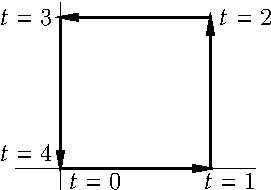
\includegraphics{figures/squarepath}
\caption{Lintasan $\gamma$ yang menelusuri persegi satuan.\label{fig:squarepath}}
\end{myfig}
\end{example}

\subsection{Integral garis}

\begin{defn}
Diberikan lintasan $C^1$ sepotong-sepotong $\gamma \colon [a,b] \to \C$ dan fungsi kontinu
$f$ pada
$\gamma$,
kita mendefinisikan \emph{\myindex{integral garis}}\footnote{%
Integral ini juga disebut
\emph{\myindex{integral lintasan}},
\emph{\myindex{integral kurva}}, atau
\emph{\myindex{integral kontur}}.}
\glsadd{not:pathint}%
\begin{equation*}
\int_{\gamma} f(z) \, dz
\overset{\text{def}}{=}
\int_a^b f\bigl(\gamma(t)\bigr) \gamma'(t) \, dt .
\end{equation*}
\end{defn}

Ruas kanan tersebut terdefinisi dengan baik.
Integrannya tidak terdefinisi
pada berhingga banyaknya titik (tempat $\gamma'(t)$ tidak ada),
tetapi integran itu kontinu sepotong-sepotong, dan hal ini cukup
agar dapat diintegralkan secara Riemann: Pada setiap interval tertutup
$[t_{\ell-1},t_\ell]$, integran tersebut dapat diperluas menjadi suatu fungsi
kontinu.
Perhatikan bahwa definisi itu terdefinisi dengan baik bahkan jika $\gamma'(t)$ nol di suatu tempat,
dan sesekali kita akan menggunakannya dalam keadaan tersebut.

Mari kita hitung contoh integral garis yang paling penting.

\begin{example} \label{example:integralpowerz}
Misalkan $\gamma \colon [0,2\pi] \to \C$ yang diberikan oleh $\gamma(t) = r e^{it}$ adalah
lingkaran berjari-jari $r$ yang berorientasi berlawanan arah jarum jam,
yakni $\partial \Delta_r(0)$.  Lihat \figureref{fig:circlepath}.
Untuk $n \in \Z$, kita menyatakan bahwa
\begin{equation*}
\int_\gamma z^n \, dz
=
\begin{cases}
2\pi i & \text{jika } n=-1, \\
0 & \text{selainnya.}
\end{cases}
\end{equation*}

\begin{myfig}
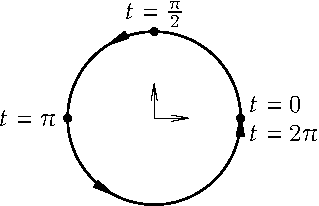
\includegraphics{figures/circlepath}
\caption{Lintasan $\gamma$ yang menelusuri lingkaran.\label{fig:circlepath}}
\end{myfig}

Pertama, $\gamma'(t) = i r e^{it}$.
Untuk membuktikan pernyataan tersebut, kita hitung
\begin{equation*}
\int_\gamma z^n \, dz
=
\int_0^{2\pi}
r^n
e^{int} i r e^{it} \, dt
=
i r^{n+1}
\int_0^{2\pi}
e^{i(n+1)t} \, dt .
\end{equation*}
Hasilnya mengikuti karena integral di ruas kanan adalah nol
(latihan di bawah), kecuali jika $n+1 = 0$,
dan dalam kasus itu integral tersebut
adalah $2\pi$ dan $r^{n+1} = 1$.  Perhatikan secara khusus bahwa nilai
integral tidak bergantung pada $r$.
\end{example}

\begin{exbox}
\begin{exercise}[Mudah]
Buktikan bahwa jika $k$ suatu bilangan bulat taknol, maka $\int_0^{2\pi} e^{ik t} \, dt = 0$.
\end{exercise}

\begin{exercise}
Misalkan $\gamma$ seperti dalam \exampleref{example:integralpowerz}
dan
$f(z) = \sum_{n=-d}^d c_n z^n$.
Hitung $\int_\gamma f(z) \, dz$.
\end{exercise}

\begin{exercise}
Hitung $\int_\gamma \bar{z}^n \, dz$ untuk semua $n \in \Z$ dan $\gamma$ seperti dalam
\exampleref{example:integralpowerz}.
\end{exercise}
\end{exbox}

Definisi integral garis kita ekuivalen dengan definisi yang
telah Anda lihat dalam kalkulus multivariabel.  Sebenarnya, definisi ini merupakan kasus khususnya.
Misalkan $\gamma(t) = x(t) +i \, y(t)$, untuk $t \in [a,b]$, adalah suatu lintasan,
dan misalkan $dz = dx + i\, dy$.
Maka
\begin{equation*}
\begin{split}
\int_{\gamma} f(z) \, dz
& =
\int_{\gamma} f(z) \, (dx + i\, dy)
\\
& =
\int_{\gamma} f(z) \, dx + i f(z) \, dy
=
\int_a^b \underbrace{\Bigl( f\bigl(\gamma(t)\bigr) x'(t) + i f\bigl(\gamma(t)\bigr) y'(t) \Bigr)}_{f(\gamma(t)) \gamma'(t)} \, dt .
\end{split}
\end{equation*}
Pada baris kedua, Anda seharusnya mengenali definisi integral garis
$\int_\gamma P\,dx + Q \, dy$ dari kalkulus.  Integral garis sebarang
di bidang dapat diperoleh jika kita juga menyertakan $d\bar{z}$.  Lihat
latihan di bawah.

\begin{exbox}
\begin{exercise} \label{exercise:realpathintegral}
\glsadd{not:dz}\glsadd{not:dzbar}%
Misalkan $dz = dx + i \, dy$ dan
$d\bar{z} = dx - i \, dy$.  Tunjukkan bahwa untuk setiap $P$ dan $Q$ kontinu (bernilai real atau kompleks),
terdapat $F$ dan $G$ kontinu (bernilai kompleks) sedemikian sehingga
\begin{equation*}
\int_{\gamma} P \, dx + Q \, dy
=
\int_{\gamma} F \, dz + G \, d\bar{z} .
\end{equation*}
Lalu tunjukkan bahwa setiap integral garis
dapat dihitung meskipun Anda hanya mengetahui cara menghitung integral berbentuk
$\int_\gamma f(z) \, dz$.
\end{exercise}
\end{exbox}

Untuk lintasan injektif, nilai integral tidak bergantung pada cara
kita memarameterkan citra lintasan tersebut,
kecuali bahwa nilainya bergantung pada orientasi (arah yang kita tempuh).
Alasannya mudah dilihat ketika
$\gamma \colon [a,b] \to \C$ terdiferensialkan secara kontinu dan kita memiliki
$h \colon [c,d] \to [a,b]$ yang terdiferensialkan secara kontinu sedemikian
sehingga $h' > 0$ (naik), $h(c)=a$, dan $h(d) = b$.  Maka $\gamma \circ h$ adalah lintasan
$C^1$ baru yang merupakan parameterisasi berbeda dari $\gamma$.
Penggantian variabel $t=h(s)$ dari kalkulus menyatakan
\begin{equation*}
\begin{split}
\int_{\gamma} f(z) \, dz
& =
\int_a^b f\bigl( \gamma(t) \bigr) \gamma'(t) \, dt
\\
& =
\int_c^d f\Bigl( \gamma\bigl(h(s)\bigr) \Bigr) \gamma'\bigl(h(s)\bigr) h'(s) \, ds
=
\int_{\gamma \circ h} f(z) \, dz.
\end{split}
\end{equation*}
Namun, jika $h' < 0$ (turun), $h(c)=b$, dan $h(d)=a$, maka
tandanya berbalik dalam penggantian variabel:
\begin{equation*}
\int_{\gamma} f(z) \, dz =
- \int_{\gamma \circ h} f(z) \, dz.
\end{equation*}

Versi umum hasil ini, yang salah satu versinya kita nyatakan di bawah,
sedikit lebih sulit dibuktikan.
Karena hasil ini, walaupun
penting secara konseptual, sebenarnya lebih merupakan persoalan teknis agar kita hanya perlu
merujuk pada citranya alih-alih parameterisasi lintasan sebenarnya, kita akan
menyerahkan buktinya sebagai latihan.

\begin{prop}[Reparameterisasi]\index{reparameterisasi lintasan}%
\label{prop:reparam}
Andaikan $\gamma \colon [a,b] \to \C$ dan $\alpha \colon [c,d] \to \C$ adalah
lintasan-lintasan $C^1$ sepotong-sepotong sedemikian sehingga
$\gamma\bigl([a,b]\bigr) = \alpha\bigl([c,d]\bigr)$.
Andaikan salah satu dari
\begin{enumerate}[(i)]
\item
$\gamma$ dan $\alpha$ injektif, atau
\item
$\gamma|_{(a,b]}$ dan
$\alpha|_{(c,d]}$ injektif dan
$\gamma(a)=\alpha(c)=\gamma(b)=\alpha(d)$ (lintasan tertutup sederhana).
\end{enumerate}
Maka terdapat fungsi kontinu monoton ketat $h \colon [c,d] \to [a,b]$ sedemikian
sehingga $\gamma\bigl(h(t)\bigr) = \alpha(t)$ untuk semua $t \in [c,d]$.
Selanjutnya:
\begin{enumerate}[(i)]
\item
Jika $h$ naik, maka untuk setiap $f$ yang kontinu pada lintasan tersebut,
\begin{equation*}
\int_\gamma f(z) \, dz = \int_{\alpha} f(z) \, dz .
\end{equation*}
\item
Jika $h$ turun, maka untuk setiap $f$ yang kontinu pada lintasan tersebut,
\begin{equation*}
\int_\gamma f(z) \, dz = - \int_{\alpha} f(z) \, dz .
\end{equation*}
\end{enumerate}
\end{prop}

\begin{exbox}
\begin{exercise}
Buktikan kasus pertama \propref{prop:reparam}.
Andaikan $\gamma$ dan $\alpha$ injektif.
\begin{exparts}
\item
Buktikan keberadaan $h$, kemonotonannya, dan kekontinuannya.
Petunjuk: Pertama, buktikan $\gamma^{-1}$ adalah fungsi kontinu pada
$\gamma\bigl([a,b]\bigr)$ dengan menggunakan fakta bahwa subhimpunan tertutup dari $[a,b]$
bersifat kompak.
\item
Buktikan proposisi tersebut untuk $f\equiv 1$.
Petunjuk: teorema dasar kalkulus.
\item
Buktikan proposisi tersebut untuk $f$ kontinu.
Petunjuk: Potong lintasan menjadi bagian-bagian kecil tempat
Anda dapat menghampiri $f$ dengan suatu konstanta dan menerapkan
bagian sebelumnya.
\end{exparts}
\end{exercise}

\begin{exercise}
Buktikan kasus kedua \propref{prop:reparam}, yakni,
untuk lintasan tertutup sederhana dengan hanya mengandaikan bahwa $\gamma|_{(a,b]}$ dan
$\alpha|_{(c,d]}$ injektif serta
$\gamma(a)=\alpha(c)=\gamma(b)=\alpha(d)$.
\end{exercise}

\begin{exercise}
Suatu lintasan $C^1$ sepotong-sepotong $\gamma \colon [a,b] \to \C$
dapat direparameterisasi menjadi suatu \myquote{lintasan} $C^1$ jika turunannya
diperbolehkan lenyap.
Artinya, terdapat fungsi kontinu naik ketat
$h \colon [a,b] \to [a,b]$ sedemikian sehingga
$\gamma \circ h$ adalah $C^1$.
Petunjuk: Jadikan turunannya nol pada \myquote{sudut-sudut.}
\end{exercise}

\begin{exercise}[Sulit]
Tinjau tak berhingga banyaknya lingkaran tersarang yang semuanya bersinggungan pada satu titik
dan misalkan titik itu adalah titik asal: Andaikan $r_n$ adalah jari-jari
lingkaran ke-$n$
dan lingkaran ke-$n$ diberikan oleh $r_n e^{i(-1)^n\theta} - r_n$, untuk $0 \leq
\theta \leq 2\pi$ (lingkaran-lingkaran tersebut ditelusuri dengan arah bergantian).
Jika $\sum r_n < \infty$, maka Anda dapat menemukan fungsi kontinu
$C^1$ $\gamma \colon
[0,1] \to \C$ yang menelusuri semua lingkaran tersebut.  Jika $\sum r_n = \infty$, maka
Anda dapat menemukan fungsi kontinu $\gamma \colon [0,1] \to \C$ yang $C^1$ pada
$(0,1]$, tetapi $\lim_{t \to 0} \gamma'(t)$ pasti tidak ada.
\end{exercise}
\end{exbox}

\begin{remark}
Dua latihan terakhir menunjukkan mengapa secara konseptual kita harus
mensyaratkan bahwa $\gamma'(t)$ tidak pernah lenyap (termasuk limit-limit sepihaknya)
untuk lintasan $C^1$ sepotong-sepotong.
Kita memandang lintasan tersebut
sebagai himpunan
$\gamma\bigl([a,b]\bigr)$,
bukan parameterisasinya, dan di tempat lintasan tersebut $C^1$,
kita menginginkannya tidak memiliki \myquote{sudut.}
Dalam praktik, kita tidak sering menggunakan persyaratan ini,
tetapi persyaratan tersebut memang membuat sejumlah argumen geometris jauh lebih sederhana.
\end{remark}

Karena hasil reparameterisasi di atas,
kita sering menuliskan \myquote{batas} suatu himpunan terbuka tertentu
(tentu saja selama batas tersebut $C^1$ sepotong-sepotong)
dan meninjau sebarang parameterisasi yang bergerak berlawanan arah jarum jam
ketika mengintegralkan di sepanjang batas itu, tanpa memberikan parameterisasinya secara eksplisit.
Sebagai contoh, diberikan cakram $\Delta_r(p)$, kita memarameterkan
batas $\partial \Delta_r(p)$ dengan
$\gamma  \colon [0,2\pi] \to \C$ yang diberikan oleh $\gamma(t) = p +
re^{it}$, lalu kita tuliskan
\glsadd{not:boundaryascycle}%
\begin{equation*}
\int_{\partial \Delta_r(p)} f(z) \, dz
=
\int_{\gamma} f(z) \, dz .
\avoidbreak
\end{equation*}
Kesamaan ini dapat langsung diambil sebagai definisi pengintegralan sepanjang
$\partial \Delta_r(p)$.

Terakhir, terdapat \myquote{substitusi-$u$} dari kalkulus.

\begin{prop} \label{prop:usubst}
Misalkan $U,V \subset \C$ terbuka, $\gamma \colon [a,b] \to V$ suatu
lintasan $C^1$ sepotong-sepotong, $g \colon V \to U$ holomorfik (andaikan $g'$
kontinu\footnote{Kita akan segera melihat bahwa $g'$ selalu kontinu.}), dan $f \colon U \to \C$
kontinu.  Maka $g \circ \gamma$ adalah lintasan $C^1$ sepotong-sepotong di $U$
(mungkin dengan turunan yang lenyap\footnote{%
Memang terdapat reparameterisasi dengan turunan taklenyap, jika kita benar-benar
sangat menginginkannya.},
namun, jika $g'$ nol pada $\gamma$) dan
\begin{equation*}
\int_{\gamma} f\bigl(g(z)\bigr) g'(z) \, dz
=
\int_{g \circ \gamma} f(w) \, dw .
\end{equation*}
\end{prop}

\begin{proof}
Jelas bahwa $g \circ \gamma$ merupakan lintasan $C^1$ sepotong-sepotong (kecuali mungkin
memiliki turunan yang lenyap).  Untuk membuktikan kesamaan tersebut,
terapkan aturan rantai,
$(g \circ \gamma)'(t) = g'\bigl(\gamma(t)\bigr) \gamma'(t)$:
\begin{equation*}
\begin{split}
\int_{\gamma} f\bigl(g(z)\bigr) g'(z) \, dz
& =
\int_a^b
f\Bigl(g\bigl(\gamma(t)\bigr)\Bigr) g'\bigl(\gamma(t)\bigr) \gamma'(t) \, dt
\\
& =
\int_a^b
f\bigl((g \circ \gamma)(t)\bigr) (g \circ \gamma)'(t) \, dt
=
\int_{g \circ \gamma} f(w) \, dw . \qedhere
\end{split}
\end{equation*}
\end{proof}

\begin{exbox}
\begin{exercise}
Misalkan $f \colon \partial \D \to \C$ suatu fungsi kontinu.  Buktikan bahwa
\begin{equation*}
\int_{\partial \D} f(z) \, dz
=
\int_{\partial \D} \frac{f\bigl(\frac{1}{z}\bigr)}{z^2} \, dz
=
\int_{\partial \D} f(\bar{z}) \bar{z}^2 \, dz .
\end{equation*}
\end{exercise}
\end{exbox}

\subsection{Integral panjang busur}

Kita juga dapat mengintegralkan terhadap panjang busur, yaitu $ds$ dari kalkulus.
Kita akan menuliskan $ds$ sebagai $\sabs{dz}$.  Untuk $f$ yang kontinu pada
lintasan $C^1$ sepotong-sepotong $\gamma \colon [a,b] \to \C$,
kita definisikan
\glsadd{not:arclength}
\begin{equation*}
\int_\gamma f(z) \, \sabs{dz}
\overset{\text{def}}{=}
\int_a^b f\bigl( \gamma(t) \bigr) \sabs{\gamma'(t)} \, dt .
\end{equation*}

%Dengan definisi ini kita dapat membuat beberapa taksiran atas integral garis.

\begin{prop}[Ketaksamaan segitiga untuk integral garis]%
\index{ketaksamaan segitiga!integral garis}
Andaikan $\gamma \colon [a,b] \to \C$ adalah
lintasan $C^1$ sepotong-sepotong dan $f$ adalah fungsi kontinu pada
$\gamma$.  Maka
\begin{equation*}
\abs{\int_\gamma f(z) \, dz} \leq \int_\gamma \sabs{f(z)} \, \sabs{dz} .
\avoidbreak
\end{equation*}
Khususnya, jika $\sabs{f(z)} \leq M$ pada $\gamma$ dan $\ell = \int_\gamma ds
= \int_{\gamma} \sabs{dz}$ adalah panjang $\gamma$, maka
\begin{equation*}
\abs{\int_\gamma f(z) \, dz} \leq M \ell .
\end{equation*}
\end{prop} 

\begin{proof}
Kita menaksir dengan menggunakan \propref{prop:inttriangleineq},
\begin{equation*}
\abs{\int_\gamma f(z) \, dz}
=
\abs{\int_a^b f\bigl( \gamma(t) \bigr) \gamma'(t) \, dt}
\leq
\underbrace{\int_a^b \abs{ f\bigl( \gamma(t) \bigr) }  \sabs{ \gamma'(t) }
\, dt}_{\int_\gamma \sabs{f(z)} \, \sabs{dz}}
\leq
M
\int_a^b \sabs{ \gamma'(t) } \, dt .
\qedhere
\end{equation*}
\end{proof}

Panjang busur tidak dipertahankan oleh konvergensi seragam lintasan.
Dengan kata lain, hanya karena citra dua lintasan sangat dekat satu sama
lain, tidak berarti integral di sepanjang keduanya akan sama.
Peringatan yang sama berlaku bagi integral $dz$ maupun integral $\sabs{dz}$.
Jadi, kita harus berhati-hati ketika mengatakan bahwa dua lintasan saling berdekatan.
Kita perlu agar turunannya juga berdekatan, karena $\gamma'$ muncul
di dalam integral.

\begin{exbox}
\begin{exercise}
\begin{exparts}
\item
Carilah barisan lintasan $C^1$ sepotong-sepotong $\gamma_n \colon [0,1] \to \C$
yang konvergen seragam menuju suatu fungsi konstan (dapat dikatakan suatu lintasan dengan
panjang nol), tetapi sedemikian sehingga $\int_{\gamma_n} \sabs{dz} \geq n$.
\item
Andaikan barisan lintasan $C^1$ $\gamma_n \colon [0,1] \to \C$
konvergen seragam menuju lintasan $C^1$ $\gamma \colon [0,1] \to \C$
sedemikian sehingga $\gamma_n'$ konvergen seragam menuju $\gamma'$, maka
$\int_{\gamma_n} \sabs{dz} \to
\int_{\gamma} \sabs{dz}$.
\end{exparts}
\end{exercise}
\end{exbox}

\subsection{Rantai}

Menggabungkan lintasan berguna dilakukan---yakni memiliki \myquote{aritmetika} lintasan tertentu.
Objek yang dihasilkan disebut \emph{rantai}, dan objek tersebut
hanyalah kombinasi formal lintasan.  Sebagai contoh, jika $\gamma$
dan $\alpha$ adalah lintasan $C^1$ sepotong-sepotong, maka rantai $\gamma+\alpha$
merupakan objek yang dapat kita integrali dengan fungsi-fungsi kontinu
pada kedua lintasan:
\begin{equation*}
\int_{\gamma + \alpha} f(z) \, dz
\overset{\text{def}}{=}
\int_{\gamma} f(z) \, dz +
\int_{\alpha} f(z) \, dz .
\end{equation*}

\begin{defn}
Suatu \emph{\myindex{rantai}} di $U \subset \C$ adalah ekspresi
\begin{equation*}
\Gamma = a_1 \gamma_1 + \cdots + a_n \gamma_n ,
\end{equation*}
dengan $a_1,\ldots,a_n \in \Z$ dan $\gamma_1,\ldots,\gamma_n$
merupakan lintasan $C^1$ sepotong-sepotong di $U$.  Kita mengintegralkan sepanjang $\Gamma$ sebagai
\glsadd{not:cycleint}%
\begin{equation*}
\int_{\Gamma} f(z) \, dz
=
\int_{a_1 \gamma_1 + \cdots + a_n \gamma_n} f(z) \, dz
\overset{\text{def}}{=}
a_1 \int_{\gamma_1} f(z) \, dz +
\cdots
+
a_n \int_{\gamma_n} f(z) \, dz .
\end{equation*}
Dua rantai $\Gamma_1$ dan $\Gamma_2$ di
$U$ disebut
\emph{ekuivalen}\index{rantai ekuivalen} (kita akan menuliskan
\glsadd{not:cycleeq}%
$\Gamma_1=\Gamma_2$) jika
\begin{equation*}
\int_{\Gamma_1} f(z) \, dz = 
\int_{\Gamma_2} f(z) \, dz
\end{equation*}
untuk semua $f \colon U \to \C$ kontinu.
Kita mendefinisikan \emph{\myindex{rantai nol}} $0$ dengan menetapkan
$\int_0 f(z) \, dz = 0$ untuk semua $f \colon U \to \C$ kontinu.
\end{defn}

Aritmetika rantai dilakukan dengan cara yang jelas sebagai jumlah formal lintasan:
Jika $\Gamma_1 = 2 \gamma_1 + \gamma_2$ dan $\Gamma_2 = 3 \gamma_2 +
\gamma_3$, maka $\Gamma_1 + \Gamma_2 = 2 \gamma_1 + 4 \gamma_2 + \gamma_3$.
Demikian pula untuk perkalian skalar: $3 \Gamma_1 = 6 \gamma_1 + 3 \gamma_2$.
\glsadd{not:cycleneg}%
Kita menuliskan $-\Gamma$ untuk $(-1)\Gamma$.
Suatu rantai $\Gamma$ ekuivalen dengan rantai nol jika
\begin{equation*}
\int_\Gamma f(z)\, dz = 0
\end{equation*}
untuk semua $f$ kontinu, dan
rantai $\Gamma_1$ dan $\Gamma_2$ ekuivalen jika $\Gamma_1 - \Gamma_2 = 0$.
Rantai dalam buku ini selalu tersusun atas lintasan $C^1$ sepotong-sepotong,
walaupun itu bukan definisi paling umum yang digunakan dalam literatur.

\begin{remark}
Untuk ekuivalensi,
himpunan tempat fungsi kontinu $f$ didefinisikan tidak terlalu penting.  Kita dapat
mengambil $f$ kontinu pada $U$, $\C$, atau hanya pada citra
$\Gamma_1$ dan $\Gamma_2$.
Menurut teorema perluasan Tietze (suatu teorema dalam setiap ruang metrik),
setiap fungsi kontinu pada subhimpunan tertutup dari
$\C$ (seperti citra $\Gamma_1$ dan $\Gamma_2$) dapat diperluas menjadi fungsi
kontinu pada $\C$.
Dengan cara kita mendefinisikan segala sesuatunya, kita tidak memerlukan Tietze.
\end{remark}

\begin{remark}
Penting bahwa definisi ekuivalensi berlaku untuk semua fungsi
kontinu.  Nanti kita akan menunjukkan bahwa jika $U$, misalnya, adalah cakram, maka untuk
setiap $\Gamma$ tertutup di $U$, $\int_\Gamma f(z) \, dz = 0$ bagi semua $f$ holomorfik.
Jelas bahwa hal itu tidak seharusnya mengakibatkan $\Gamma$ ekuivalen dengan rantai
nol.
Lihat pula \exerciseref{exercise:nonconstantnonzerochain}.
\end{remark}

\begin{exbox}
\begin{exercise}%[\neededexmark]
\label{exercise:pathsum}
Misalkan $\gamma_1 \colon [a,b] \to \C$ dan $\gamma_2 \colon [b,c] \to \C$
adalah dua lintasan $C^1$ sepotong-sepotong dan $\gamma_1(b)=\gamma_2(b)$.
Buktikan bahwa fungsi $\gamma \colon [a,c] \to
\C$ yang didefinisikan oleh $\gamma(t) = \gamma_1(t)$ jika $t \in [a,b]$ dan $\gamma(t)
= \gamma_2(t)$ jika $t \in [b,c]$ merupakan lintasan $C^1$ sepotong-sepotong, dan
untuk semua $f$ yang kontinu pada citra $\gamma$, berlaku
\begin{equation*}
\int_{\gamma} f(z)\,dz = \int_{\gamma_1 + \gamma_2} f(z) \, dz .
\end{equation*}
\end{exercise}

\begin{exercise}
Misalkan $\partial \D$ menyatakan lintasan berlawanan arah jarum jam mengelilingi cakram satuan.
Tunjukkan bahwa untuk setiap bilangan bulat taknol $n$, rantai $n \partial \D$ ekuivalen dengan
lintasan $\gamma \colon [0,2\pi] \to \C$ yang diberikan oleh $\gamma(t) = e^{int}$,
yaitu lintasan yang mengelilingi cakram satuan $n$ kali berlawanan arah jarum jam.
\end{exercise}

\begin{exercise} \label{exercise:nonconstantnonzerochain}
\begin{exparts}
\item
Andaikan $U \subset \C$ terbuka dan
$\gamma \colon [a,b] \to U$
adalah lintasan $C^1$
sepotong-sepotong dan $\gamma|_{[a,b)}$ injektif, tetapi mungkin merupakan lintasan tertutup,
sehingga mungkin $\gamma(a)=\gamma(b)$.  Tunjukkan bahwa sebagai rantai, $\gamma$ tidak ekuivalen dengan rantai nol.
Catatan: $\gamma$ tertutup lebih sulit.
\item
Carilah lintasan $C^1$ sepotong-sepotong $\gamma \colon [a,b] \to \C$
yang ekuivalen dengan rantai nol.  Perhatikan bahwa definisi kita tentang
\myquote{lintasan}
mencegah $\gamma$ menjadi konstan.
\end{exparts}
\end{exercise}
\end{exbox}

Dengan menggunakan \exerciseref{exercise:pathsum},
setiap rantai yang disusun
dari lintasan-lintasan yang tersambung dapat diubah dan diintegralkan sebagai satu lintasan,
sehingga selanjutnya kita dapat melakukan prosedur ini secara implisit.

\begin{defn}
\pagebreak[2]
\glsadd{not:segment}%
Diberikan dua titik $z,w \in \C$, \emph{\myindex{segmen}} $[z,w]$ adalah lintasan
$\gamma \colon [0,1] \to \C$ yang diberikan oleh $\gamma(t) = (1-t)z + tw$.
Untuk keperluan aritmetika rantai, $-[z,w] = [w,z]$.
Suatu lintasan disebut \emph{\myindex{poligonal}} jika dapat dituliskan sebagai
(ekuivalen dengan) suatu rantai
$[z_1,z_2] + [z_2,z_3] + \cdots + [z_{k-1},z_k]$ untuk sejumlah bilangan kompleks
$z_1,\ldots,z_k$.
\end{defn}

Seperti ditunjukkan latihan berikut, jika kita menginginkannya, untuk kebanyakan keperluan praktis
kita cukup menggunakan lintasan poligonal.
Bagaimanapun, lintasan yang muncul dalam penerapan sering dibangun dari
segmen dan busur.

\begin{exbox}
\begin{exercise}[Sulit]
Andaikan $U \subset \C$ terbuka, $\gamma \colon [a,b] \to U$ adalah
lintasan $C^1$ sepotong-sepotong, dan $f \colon U \to \C$ kontinu.  Maka untuk setiap $\epsilon
> 0$, terdapat lintasan (atau rantai) poligonal $\alpha$ di $U$ dengan titik
awal dan akhir yang sama sedemikian sehingga
\begin{equation*}
\abs{\int_\alpha f(z)\, dz - \int_{\gamma} f(z) \, dz} < \epsilon .
\avoidbreak
\end{equation*}
Petunjuk: Tinjau jumlah Riemann.  Selain itu, $f$ kontinu seragam pada suatu
$U$ yang lebih kecil.
\end{exercise}
\end{exbox}

%%%%%%%%%%%%%%%%%%%%%%%%%%%%%%%%%%%%%%%%%%%%%%%%%%%%%%%%%%%%%%%%%%%%%%%%%%%%%%

\section{Versi awal teorema Cauchy}
\label{sec:simplecauchy}

\subsection{Primitif, siklus, dan teorema Cauchy untuk turunan}

\begin{defn}
Misalkan $U \subset \C$ terbuka dan $f \colon U \to \C$
suatu fungsi.  Fungsi holomorfik $F \colon U \to \C$ dengan $f = F'$
disebut suatu (fungsi holomorfik)\footnote{%
Kita biasanya cukup mengatakan \myquote{primitif} karena umumnya jelas bahwa fungsi tersebut harus berupa
primitif holomorfik, dan lagi pula, itulah satu-satunya cara kita akan menggunakan
istilah tersebut.}
\emph{\myindex{primitif}}\index{primitif holomorfik} (atau suatu \emph{\myindex{antiturunan}})
dari $f$.
\end{defn}

Primitif tidak selalu ada, tetapi jika ada, maka primitif tersebut tunggal hingga
penambahan suatu konstanta.

\begin{prop} \label{prop:primunique}
Misalkan $U \subset \C$ adalah sebuah domain, dan
$F \colon U \to \C$ serta
$G \colon U \to \C$ adalah fungsi-fungsi holomorfik sedemikian sehingga $F' = G'$.  Maka
terdapat suatu konstanta $C$ sedemikian sehingga
$F(z) = G(z) + C$.
\end{prop}

\begin{exbox}
\begin{exercise}
Buktikan proposisi tersebut.
Pastikan Anda menggunakan fakta bahwa $U$ adalah sebuah domain (terhubung).
\end{exercise}
\end{exbox}

Kita telah memiliki antiturunan.  Kita telah memiliki integral.  Kita memerlukan
sebuah teorema dasar.

\begin{thm}[Teorema dasar kalkulus untuk integral garis]
\index{teorema dasar kalkulus!integral garis}%
Misalkan $U \subset \C$ terbuka dan $f \colon U \to \C$
kontinu dengan suatu primitif $F \colon U \to \C$ (jadi $F' = f$).
Misalkan $\gamma \colon [a,b] \to U$ merupakan lintasan $C^1$ sepotong-sepotong.
Maka
\begin{equation*}
\int_\gamma f(z) \, dz =
F\bigl( \gamma(b) \bigr) - F\bigl( \gamma(a)
\bigr) .
\end{equation*}
\end{thm}

\begin{proof}
Kita hitung:
\begin{equation*}
\int_\gamma F'(z) \, dz
=
\int_a^b F'\bigl(\gamma(t)\bigr) \gamma'(t) \, dt 
=
\int_a^b \frac{d}{dt} \Bigl( F\bigl(\gamma(t)\bigr) \Bigr) \, dt 
=
F\bigl( \gamma(b) \bigr) - F\bigl( \gamma(a) \bigr) .
\end{equation*}
Perhitungan ini menggunakan aturan rantai (\propref{prop:chainrule2})
dan teorema dasar kalkulus, dengan
teorema dasar kalkulus standar (real) diterapkan pada bagian real dan imajiner
dari ekspresi tersebut.
\end{proof}

\begin{remark}
Hipotesis bahwa $f=F'$ kontinu sebenarnya tidak diperlukan.
Kita akan segera membuktikan bahwa turunan suatu fungsi holomorfik bersifat
holomorfik.  Karena hal itu belum dibuktikan, kita memerlukan $F'$ setidaknya
kontinu agar integralnya terdefinisi.\footnote{%
Suatu turunan real mungkin hanya dapat diintegralkan
dengan apa yang disebut integral tolok atau Henstock--Kurzweil---integral Riemann atau
bahkan Lebesgue tidak memadai---sehingga keterintegralan bukanlah persoalan sepele.
Jika pembaca bersedia memburu semut dengan palu godam, maka
pernyataan dan bukti proposisi tersebut sepenuhnya sah pada tahap ini
jika integral tolok digunakan, bahkan tanpa hipotesis apa pun pada $f$.}
\end{remark}

\begin{defn}
Suatu rantai $\Gamma$ 
disebut sebuah \emph{\myindex{siklus}} jika
rantai tersebut ekuivalen dengan
$a_1 \gamma_1 + \cdots + a_n \gamma_n$, dengan $\gamma_1, \ldots, \gamma_n$
merupakan lintasan-lintasan tertutup $C^1$ sepotong-sepotong
dan $a_1,\ldots,a_n \in \Z$.
\end{defn}

Ingat bahwa lintasan $\gamma \colon [a,b] \to \C$ tertutup jika $\gamma(a) = \gamma(b)$.
Perhatikan bahwa kita tidak mengatakan $\Gamma$ \emph{merupakan} jumlah lintasan
tertutup, melainkan bahwa rantai itu
\emph{ekuivalen dengan} jumlah lintasan tertutup.  Lintasan persegi dalam
\exampleref{example:squarepath} merupakan suatu siklus, dan dapat ditulis dengan lebih
praktis sebagai rantai yang tersusun atas empat ruas garis lurus $[0,1] +
[1,1+i]+[1+i,i]+[i,0]$.
Teorema dasar tersebut memiliki akibat langsung
berikut.

\begin{cor}[Teorema Cauchy untuk turunan] \label{cor:cauchyforders}
\index{teorema Cauchy!untuk turunan}%
Misalkan $U \subset \C$ terbuka dan $f \colon U \to \C$
kontinu dengan suatu primitif
$F \colon U \to \C$.
Misalkan $\Gamma$ merupakan
suatu siklus
di $U$.
Maka
\begin{equation*}
\int_\Gamma f(z) \, dz = 0 .
\end{equation*}
\end{cor}

Kita akan membuktikan beberapa versi teorema Cauchy, meskipun versi ini
agak berbeda dari yang lain.  Biasanya akan terdapat pembatasan pada
$U$ atau mungkin pada lintasan atau siklus $\Gamma$,
sedangkan fungsinya biasanya cukup berupa sebarang fungsi holomorfik.
Suatu versi teorema Cauchy dapat dipandang sebagai hasil \myquote{ketaktergantungan terhadap lintasan}
yang mengatakan bahwa kita dapat mendefinisikan suatu fungsi di $z$ melalui integral garis
dari suatu titik tetap menuju $z$.  Hasilnya adalah bahwa fungsi tersebut merupakan
suatu primitif.  Jadi, versi-versi lain teorema Cauchy secara umum akan
membatasi $\Gamma$ mana yang dapat digunakan atau
membatasi hanya pada $U$ yang setiap fungsi holomorfiknya memiliki suatu primitif.

Akibat berikut akan sepenuhnya
tercakup dalam versi Cauchy yang lebih umum yang akan kita buktikan nanti,
tetapi saat ini hasil tersebut cukup menarik.

\begin{cor}[Teorema Cauchy untuk polinomial] \label{cor:cauchyforpoly}
\index{teorema Cauchy!untuk polinomial}%
Misalkan $P(z)$ adalah suatu polinomial dan $\Gamma$ merupakan
suatu siklus (di $\C$).
Maka
\begin{equation*}
\int_\Gamma P(z) \, dz = 0 .
\end{equation*}
\end{cor}

\begin{exbox}
\begin{exercise}
Buktikan teorema Cauchy untuk polinomial.
\end{exercise}

\begin{exercise}
Misalkan $f$ diberikan oleh deret pangkat di $p$ yang konvergen di $\Delta_R(p)$.  Misalkan
$\Gamma$ merupakan suatu siklus di $\Delta_R(p)$.  Buktikan bahwa
\begin{equation*}
\int_\Gamma f(z) \, dz = 0 .
\avoidbreak
\end{equation*}
% This makes it too easy
%Hint: \exerciseref{exercise:antidefpowerser}.
\end{exercise}

\begin{exercise}
Misalkan $U \subset \C$ terbuka, $f \colon U \to \C$ holomorfik, dan
$\Gamma$ merupakan suatu siklus di $U$.  
Untuk suatu $p \in U$, carilah fungsi holomorfik $g \colon U \to \C$ dengan $g(p) = 0$
dan $g'(p) = 0$ sedemikian sehingga $\int_\Gamma g(z)\, dz = \int_\Gamma f(z) \, dz$.
\end{exercise}

\begin{exercise}
Misalkan $n \neq -1$ suatu bilangan bulat dan $\Gamma$ suatu siklus di $\C \setminus \{ 0 \}$.
Hitung
\begin{equation*}
\int_\Gamma z^n \, dz .
\end{equation*}
\end{exercise}

\begin{exercise}
Dengan menggunakan \exampleref{example:integralpowerz}, tunjukkan bahwa $\nicefrac{1}{z}$
tidak memiliki primitif di $\C \setminus \{ 0 \}$.
\end{exercise}
\end{exbox}

\subsection{Cauchy--Goursat, \myquote{Cauchy untuk segitiga}}

\begin{defn}
Suatu himpunan $X$ disebut \emph{\myindex{konveks}} jika ruas $[a,b] \subset X$ untuk semua $a,b \in
X$.
Misalkan $a,b,c \in \C$ merupakan titik-titik berbeda di $\C$ yang tidak terletak pada
satu garis lurus.
Suatu \emph{\myindex{segitiga}} $T$
dengan titik-titik sudut $a,b,c$ adalah selubung konveks
dari $\{ a,b,c \}$, yaitu
himpunan semua titik
\begin{equation*}
t_1 a + t_2 b + t_3 c ,
\avoidbreak
\end{equation*}
dengan $t_1,t_2,t_3 \in [0,1]$ dan $t_1+t_2+t_3 = 1$.
\end{defn}

Cara lain untuk mendefinisikan
selubung konveks adalah sebagai irisan semua himpunan konveks yang memuat $\{ a,b,c \}$.
Secara khusus, $T$ adalah himpunan konveks terkecil yang memuat titik-titik sudut tersebut.
Perhatikan bahwa kita telah mendefinisikan segitiga sebagai segitiga penuh, termasuk
bagian dalamnya.

\begin{myfig}
\subimport*{figures/}{triang.pdf_t}
\caption{Segitiga yang berorientasi positif.%
\label{fig:triang}}
\end{myfig}
Urutkan titik-titik sudut sehingga batas $\partial T$ memiliki orientasi positif;
jika kita bergerak dari $a$ ke $b$ lalu ke $c$, bagian dalam segitiga 
berada di sebelah kiri.  Lebih tepatnya, jika kita mentranslasikan sehingga $a$ menjadi
titik asal dan merotasikan sehingga $b$ berada pada garis real positif, maka $c$
memiliki bagian imajiner positif.  Lihat \figureref{fig:triang}.  Definisikan siklus batas
dari $T$ sebagai
\begin{equation*}
\partial T = [a,b] + [b,c] + [c,a] .
\end{equation*}

\begin{thm}[Cauchy--Goursat\footnote{%
Yang menjadikan teorema ini teorema Goursat
dan bukan sekadar pernyataan lain teorema Cauchy
adalah bahwa dalam buktinya kita hanya mengasumsikan turunan kompleks ada,
bukan bahwa turunan itu kontinu, seperti yang diasumsikan
oleh Cauchy.}]\index{teorema Cauchy--Goursat}\label{thm:cauchygoursat}
\pagebreak[2]
Misalkan $U \subset \C$ terbuka, $f \colon U \to \C$
holomorfik,
dan $T \subset U$ merupakan suatu segitiga.  Maka
\begin{equation*}
\int_{\partial T} f(z) \, dz = 0 .
\end{equation*}
\end{thm}

Penting bahwa $T \subset U$ berarti bagian dalam
segitiga berada di $U$, bukan hanya batasnya.  Jika tidak, teorema tersebut
tidak akan benar.

\begin{proof}
Kita bekerja dengan kontraposisi.
Misalkan $f$ kontinu, dan 
misalkan terdapat suatu segitiga $T \subset U$ yang integral sepanjang batasnya tidak nol.
Tuliskan
\begin{equation*}
\abs{\int_{\partial T} f(z) \, dz} = c > 0 .
\end{equation*}
Kita akan menemukan suatu titik
tempat $f$ tidak terdiferensialkan secara kompleks.

Bagi $T$ menjadi empat subsegitiga
$T_1$, $T_2$, $T_3$, $T_4$ dengan membagi setiap sisi $T$ menjadi dua bagian sama panjang.  Lihat
\figureref{fig:trianggoursat}.
\begin{myfig}
\subimport*{figures/}{trianggoursat.pdf_t}
\caption{Membagi sebuah segitiga menjadi empat segitiga berukuran setengah.%
\label{fig:trianggoursat}}
\end{myfig}

Setiap $T_j$ berorientasi positif.
Sisi-sisi segitiga bagian dalam $T_4$ memiliki orientasi yang berlawanan
dengan orientasi sisi-sisi dalam $T_1$, $T_2$, dan $T_3$, sehingga
integral-integral garis pada sisi-sisi tersebut saling meniadakan.  Oleh karena itu,
\begin{equation*}
c = 
\abs{\int_{\partial T} f(z) \, dz }
=
\abs{\int_{\partial T_1} f(z) \, dz 
+
\int_{\partial T_2} f(z) \, dz 
+
\int_{\partial T_3} f(z) \, dz 
+
\int_{\partial T_4} f(z) \, dz } .
\end{equation*}
Salah satu dari keempat integral tersebut, katakanlah integral pada $\partial T_j$,
harus memiliki modulus setidaknya $\nicefrac{c}{4}$.  Beri label
segitiga tersebut $T^1 = T_j$:
\begin{equation*}
\abs{\int_{\partial T^1} f(z) \, dz } \geq \frac{c}{4} .
\end{equation*}
Sekarang bagi $T^1$ menjadi subsegitiga
$T_1^1$, $T_2^1$, $T_3^1$, $T_4^1$ seperti di atas dan ulangi prosedur tersebut.  Terdapat
salah satu dari keempatnya yang integralnya setidaknya $\frac{c}{4^2}$; beri label
$T^2$.  Ulangi terus.
Secara keseluruhan, untuk segitiga ke-$k$, yaitu $T^k$,
\begin{equation*}
\abs{\int_{\partial T^k} f(z) \, dz } \geq \frac{c}{4^k} .
\end{equation*}
Selain itu, $T^k \subset T^{k-1} \subset \cdots \subset T$.
Pada setiap langkah, seluruh subsegitiga merupakan segitiga-segitiga sebangun (sudutnya sama),
tetapi panjang sisinya tepat dibagi dua.
Secara khusus,
jarak terbesar yang mungkin antara dua titik dalam segitiga 
terbagi dua pada setiap iterasi.
Dalam bahasa yang lebih formal:\footnote{%
Di sini $\operatorname{diam}(T)= \sup \{ \sabs{p-q} : p,q \in T \}$
berarti jarak maksimum antara dua titik di $T$.}
\begin{equation*}
\operatorname{diam}(T^k) =
\frac{1}{2} \operatorname{diam}(T^{k-1})
=
\frac{1}{2^k} \operatorname{diam}(T) .
\end{equation*}
Karena $T$ kompak dan setiap $T^k$ tertutup, irisan bersarang dari $T^k$ harus takkosong.
Karena diameternya menuju nol, irisan tersebut harus berupa satu titik:
\begin{equation*}
\{ z_0 \} = \bigcap_{k=1}^\infty T^k .
\end{equation*}

Untuk suatu $\alpha \in \C$, definisikan $g$ melalui
\begin{equation*}
f(z) = f(z_0) + \alpha (z-z_0) + g(z) .
\end{equation*}
Seandainya $f$ terdiferensialkan secara kompleks di $z_0$, akan terdapat suatu $\alpha$ sehingga
$\frac{g(z)}{z-z_0}$ menuju nol ketika $z \to z_0$.
Mari kita buktikan bahwa hal itu tidak menuju nol untuk sebarang $\alpha$.  Tetapkan $\alpha$
dan dengan demikian $g$.
\hyperref[cor:cauchyforpoly]{Teorema Cauchy untuk polinomial} menyatakan
\begin{equation*}
\int_{\partial T^k} f(z) \, dz =
\int_{\partial T^k} \bigl( f(z_0) + \alpha (z-z_0) + g(z) \bigr) \, dz =
\int_{\partial T^k} g(z) \, dz .
\end{equation*}
Dengan demikian,
\begin{equation*}
\frac{c}{4^k} \leq
\abs{
\int_{\partial T^k} f(z) \, dz
} =
\abs{
\int_{\partial T^k} g(z) \, dz 
}
\leq
\int_{\partial T^k} \sabs{g(z)} \, \sabs{dz} .
\end{equation*}
Misalkan $\ell$ adalah jumlah panjang sisi-sisi $T$.
Jumlah panjang sisi-sisi $T^k$ adalah
$\frac{\ell}{2^k}$.
Menurut teorema nilai rata-rata untuk integral\footnote{%
Jika $\varphi \colon [a,b] \to \R$ kontinu, maka terdapat $x \in [a,b]$
sedemikian sehingga $\varphi(x) = \frac{1}{b-a} \int_a^b \varphi(t) \, dt$.
Untuk menerapkannya di sini, parametrisasi batas segitiga $\partial T^k$ dengan laju satuan.},
terdapat $z_k \in \partial T^k$ sedemikian sehingga
\begin{equation*}
\sabs{g(z_k)} = 
\frac{2^k}{\ell}
\int_{\partial T^k} \sabs{g(z)} \, \sabs{dz} .
\end{equation*}
Kita mempunyai $z_k \neq z_0$ karena $g(z_0)=0$
dan $\sabs{g(z_k)} \geq \frac{c}{\ell 2^k} > 0$.
Misalkan $d = \operatorname{diam}(T)$.  Maka
$\sabs{z_k-z_0} \leq \frac{d}{2^k}$ dan
\begin{equation*}
\abs{\frac{g(z_k)}{z_k-z_0}}
\geq
\frac{2^k\sabs{g(z_k)}}{d}
=
\frac{4^k}{d \ell}
\int_{\partial T^k} \sabs{g(z)} \, \sabs{dz}
\geq
\frac{4^k}{d \ell}
\frac{c}{4^k} = \frac{c}{d \ell} .
\end{equation*}
Karena $z_k \to z_0$, kita memperoleh bahwa $\frac{g(z)}{z-z_0}$ tidak 
menuju nol ketika $z \to z_0$.  Jadi $f$ tidak terdiferensialkan secara kompleks di $z_0$.
\end{proof}

\begin{exbox}
\begin{exercise}
Misalkan $T \subset \C$ adalah suatu segitiga dan $f \colon T \to \C$ suatu
fungsi kontinu yang pembatasannya pada interior $T$ holomorfik.
Buktikan bahwa $\int_{\partial T} f(z) \, dz = 0$.
\end{exercise}

\begin{exercise}
Suatu persegi panjang tertutup $R \subset \C$ adalah himpunan
$\bigl\{ z \in \C : a \leq \Re z \leq b , c \leq \Im z \leq d \bigr\}$
untuk bilangan-bilangan real $a < b$, $c < d$.  Batasnya
kembali diorientasikan berlawanan arah jarum jam.  Buktikan Cauchy--Goursat untuk persegi panjang
(gantikan $T$ dalam teorema dengan $R$).
\end{exercise}

\begin{exercise}
Misalkan $R$ merupakan persegi panjang dengan titik-titik sudut
$-1-i$, $1-i$, $1+i$, dan $-1+i$, serta perhatikan bahwa $0$ berada di interiornya.
Hitung $\int_{\partial R} \frac{1}{z} \, dz$,
perhatikan bahwa hasilnya tidak nol, dan jelaskan mengapa hal itu tidak melanggar
teorema Cauchy--Goursat untuk persegi panjang (lihat latihan sebelumnya).
Petunjuk: Kita belum memiliki logaritma kompleks, jadi Anda tidak dapat menggunakannya,
tetapi perhatikan, misalnya:
$\frac{1}{t-i} = \frac{t}{t^2+1} + i \frac{1}{t^2+1}$.
\end{exercise}
\end{exbox}

Segitiga adalah salah satu jenis himpunan konveks, tetapi karena himpunan konveks sering
muncul, mari kita berikan beberapa sifat dasar himpunan konveks sebagai latihan.
Latihan-latihan ini sebaiknya dikerjakan secara berurutan dan hasil sebelumnya mungkin dapat digunakan untuk menyelesaikan
latihan-latihan berikutnya.

\begin{exbox}
\begin{exercise}
Buktikan:
\begin{exparts}
\item
Irisan sebarang dari himpunan-himpunan konveks bersifat konveks.
\item
Interior suatu himpunan konveks bersifat konveks.
\item
Penutupan suatu himpunan konveks bersifat konveks.
\end{exparts}
\end{exercise}

\begin{exercise}
Misalkan $X \subset \C$ suatu himpunan konveks dan $\xi \in \partial X$; buktikan bahwa
terdapat $w$ taknol sedemikian sehingga untuk semua $z \in X$, berlaku
\begin{equation*}
\Re z\bar{w} \geq \Re \xi\bar{w} .
\end{equation*}
Dengan kata lain, $X$ berada dalam setengah bidang tertutup
yang dibatasi oleh suatu garis lurus yang memuat $\xi$ dan
ortogonal terhadap $w$.
Perhatikan bahwa $\Re z\bar{w}$ adalah hasil kali titik standar dari
kalkulus vektor di $\R^2$.
\end{exercise}

\begin{exercise}
Misalkan $X \subset \C$ suatu himpunan konveks tertutup.
Buktikan bahwa $X$ merupakan irisan setengah bidang tertutup (lihat
latihan sebelumnya).
\end{exercise}

\begin{exercise}
Gabungan himpunan-himpunan konveks biasanya tidak konveks, tetapi jika $\{ X_n \}$ merupakan
barisan himpunan konveks sedemikian sehingga $X_n \subset X_{n+1}$, maka
buktikan bahwa gabungan $\bigcup_n X_n$ bersifat konveks.
\end{exercise}
\end{exbox}

\subsection{Cauchy untuk himpunan berbentuk bintang}

\begin{defn}
Suatu himpunan $U \subset \C$ disebut \emph{\myindex{berbentuk bintang}} (atau lebih tepatnya
\emph{berbentuk bintang terhadap $z_0$}) jika terdapat suatu
titik $z_0 \in U$ sedemikian sehingga ruas $[z_0,z] \subset U$ untuk setiap
$z \in U$.  Lihat \figureref{fig:starshaped}.
\end{defn}

\begin{myfig}
\subimport*{figures/}{starshaped.pdf_t}
\caption{Suatu domain yang berbentuk bintang terhadap $z_0$.\label{fig:starshaped}}
\end{myfig}

Suatu himpunan konveks berbentuk bintang, tetapi kebalikannya tidak selalu benar.

\begin{exbox}
\begin{exercise}%[\neededexmark]
\label{exercise:triangleinstarlike}
Buktikan bahwa jika $U \subset \C$ berbentuk bintang terhadap $z_0$ dan $[a,b]
\subset U$, maka segitiga $T$ dengan titik-titik sudut $z_0$, $a$, dan $b$ seluruhnya
termuat dalam $U$.
\end{exercise}

\begin{exercise}
Misalkan $U \subset \C$ terbuka dan berbentuk bintang.  Buktikan bahwa $U$ terhubung.
\end{exercise}

\begin{exercise}
\begin{exparts}
\item
Buktikan bahwa jika $U_1,\ldots,U_n \subset \C$ konveks dan $U_1 \cap 
\cdots \cap U_n \neq \emptyset$, maka gabungan $U_1 \cup \cdots \cup U_n$
berbentuk bintang.
\item
Carilah contoh $U_1,U_2,U_3 \subset \C$ yang konveks dengan
$U_1 \cap U_2 \neq \emptyset$,
$U_1 \cap U_3 \neq \emptyset$, dan
$U_2 \cap U_3 \neq \emptyset$, tetapi sedemikian sehingga $U_1 \cup U_2 \cup U_3$
tidak berbentuk bintang.
\end{exparts}
\end{exercise}
\end{exbox}

\begin{prop} \label{prop:primitiveinstarlike1}
Misalkan $U \subset \C$ terbuka dan berbentuk bintang,
$f \colon U \to \C$ kontinu, dan
\begin{equation*}
\int_{\partial T} f(z) \, dz = 0
\end{equation*}
untuk setiap segitiga $T \subset U$.
Maka $f$ memiliki suatu primitif, yaitu
terdapat fungsi holomorfik $F \colon U \to \C$
sedemikian sehingga $F' = f$.
\end{prop}

\begin{proof}
Misalkan $U$ berbentuk bintang terhadap $z_0 \in U$.
Untuk $z \in U$, definisikan
\begin{equation*}
F(z) = \int_{[z_0,z]} f(\zeta) \, d\zeta .
\end{equation*}

Perhatikan suatu cakram kecil $\Delta_r(z) \subset U$.
Jika $\sabs{h} < r$, maka
$z+h \in \Delta_r(z)$.
Garis antara $z$ dan $z+h$ berada di $U$, dan
karena $U$ berbentuk bintang terhadap $z_0$, 
seluruh segitiga (atau ruas garis jika titik-titik tersebut segaris)
dengan titik-titik sudut $z_0$, $z$, dan $z+h$
berada di $U$; lihat \figureref{fig:triangantidef}
(dan \exerciseref{exercise:triangleinstarlike}).
\begin{myfig}
\subimport*{figures/}{triangantidef.pdf_t}
\caption{Domain berbentuk bintang dan segitiga dengan titik-titik sudut
$z_0$, $z$, dan $z+h$.\label{fig:triangantidef}}
\end{myfig}

Hipotesis menyatakan (dan ini benar secara trivial jika titik-titiknya segaris)
\begin{equation*}
\int_{[z_0,z]+[z,z+h]-[z_0,z+h]} f(\zeta) \, d\zeta = 0 .
\end{equation*}
Jadi
\begin{equation*}
\begin{split}
\frac{F(z+h)-F(z)}{h} &=
\frac{1}{h}
\int_{[z_0,z+h]-[z_0,z]} f(\zeta) \, d\zeta
\\
& =
\frac{1}{h}
\int_{[z,z+h]} f(\zeta) \, d\zeta
=
\frac{1}{h}
\int_0^1 f(z+th) h \, dt
=
\int_0^1 f(z+th) \, dt .
\end{split}
\end{equation*}
Dengan kata lain,
\begin{equation*}
\begin{split}
\abs{
\frac{F(z+h)-F(z)}{h} 
-
f(z)
}
& =
\abs{
\int_0^1 f(z+th) \, dt
-
\int_0^1 f(z) \, dt
}
\\
& \leq
\int_0^1 \abs{f(z+th)-f(z)} \, dt .
\end{split}
\end{equation*}
Menurut kekontinuan $f$ di $z$,
\begin{equation*}
\lim_{h \to 0}
\frac{F(z+h)-F(z)}{h} 
=
f(z) . \qedhere
\end{equation*}
\end{proof}

Cauchy--Goursat (\thmref{thm:cauchygoursat}) menyatakan bahwa integral mengelilingi
segitiga selalu nol jika $f$ holomorfik.  Dengan demikian, kita memperoleh
akibat langsung berikut.

\begin{cor} \label{cor:primitiveinstarlike}
Misalkan $U \subset \C$ terbuka dan berbentuk bintang
dan $f \colon U \to \C$ holomorfik.
Maka $f$ memiliki suatu primitif, yaitu
terdapat fungsi holomorfik $F \colon U \to \C$
sedemikian sehingga $F' = f$.
\end{cor}

Kita juga memperoleh akibat lain, yang kita sebut
teorema karena merupakan salah satu hasil fundamental.

\begin{thm}[Teorema Cauchy untuk domain berbentuk bintang]
\index{teorema Cauchy!domain berbentuk bintang}%
Misalkan $U \subset \C$ terbuka dan berbentuk bintang, $f \colon U \to \C$ holomorfik,
dan $\Gamma$ merupakan
suatu siklus
di $U$.  Maka
\begin{equation*}
\int_{\Gamma} f(z) \, dz = 0 .
\end{equation*}
\end{thm}

\begin{proof}
\corref{cor:primitiveinstarlike} mengimplikasikan bahwa terdapat
suatu primitif $F \colon U \to \C$.
Teorema Cauchy untuk turunan (\corref{cor:cauchyforders}) kemudian mengimplikasikan bahwa integral tersebut nol.
\end{proof}

\begin{exbox}
\begin{exercise}
Misalkan $f \colon \C \setminus \{ 0 \} \to \C$ holomorfik
dan
$\gamma \colon [a,b] \to \C \setminus \{ 0 \}$ merupakan lintasan tertutup $C^1$ sepotong-sepotong
sedemikian sehingga $\Re \gamma(t) < \sabs{\gamma(t)}$ untuk semua $t \in [a,b]$.
Tunjukkan bahwa $\int_\gamma f(z) \, dz = 0$.
\end{exercise}

\begin{exercise}
Misalkan $\gamma$ adalah setengah lingkaran atas dari lingkaran satuan yang diorientasikan dari $1$ ke
$-1$.   Misalkan $f \colon \C \to \C$ holomorfik
dan $\int_0^1 f(x^2) \, dx = \pi$.
Hitung $\int_\gamma f(z^2) \, dz$.
\end{exercise}

\begin{exercise}
Misalkan $U_1, U_2 \subset \C$ merupakan domain berbentuk bintang sedemikian sehingga $U_1 \cap U_2$
takkosong dan terhubung.  Buktikan teorema Cauchy untuk $U = U_1 \cup U_2$, yaitu,
jika $f \colon U \to \C$ holomorfik dan $\Gamma$ suatu siklus di $U$,
maka $\int_\Gamma f(z) \, dz = 0$.
\end{exercise}

\begin{exercise}
Misalkan $U \subset \C$ terbuka dan berbentuk bintang serta
$f \colon U \to \C$ antiholomorfik, yaitu konjugat dari suatu
fungsi holomorfik.  Misalkan $d\bar{z} = dx - i \, dy$ seperti sebelumnya.  Misalkan
$\Gamma$ merupakan suatu siklus di $U$.  Buktikan bahwa
$\int_\Gamma f(z) \, d\bar{z} = 0$.
\end{exercise}
\end{exbox}

\begin{remark}\label{remark:irrotvfield}
Fungsi bernilai kompleks dapat dipandang sebagai suatu medan vektor pada $\R^2$.
\corref{cor:primitiveinstarlike}
sebenarnya merupakan kasus khusus dari suatu teorema yang telah Anda jumpai
dalam kalkulus vektor, yakni suatu versi \emph{\myindex{lema Poincar\'e}}:
\emph{Dalam suatu domain berbentuk bintang $U \subset \R^2$, jika suatu
medan vektor $C^1$, $(u,v) \colon U \to \R^2$,
memenuhi $\frac{\partial u}{\partial y} = \frac{\partial v}{\partial x}$
(medan vektor tersebut \emph{takberotasi}\index{medan vektor takberotasi}),
maka terdapat fungsi bernilai real $f \colon \R^2 \to \R$ sedemikian sehingga
$\nabla f = (u,v)$ (medan vektor tersebut konservatif, yakni suatu gradien).}
Secara lebih ringkas, \emph{suatu medan vektor takberotasi
dalam domain berbentuk bintang bersifat konservatif.}
Lihat bagian \myquote{medan vektor konservatif}
dalam buku teks kalkulus favorit Anda.  Anda dapat memperoleh banyak
intuisi mengenai materi fungsi holomorfik saat ini dengan meninjau kembali
analog-analog dalam kalkulus vektor.
\end{remark}

\begin{exbox}
\begin{exercise}
Gunakan hasil tentang medan vektor takberotasi dari
\remarkref{remark:irrotvfield} untuk membuktikan 
\corref{cor:primitiveinstarlike}.
Asumsikan Anda mengetahui bahwa fungsi holomorfik adalah $C^1$.
\end{exercise}
\end{exbox}

\subsection{Rumus Cauchy dalam suatu cakram}

Barangkali teorema paling fundamental dalam analisis kompleks satu variabel,
dan akar dari semua sifat menakjubkan fungsi holomorfik,
adalah rumus integral Cauchy.  Mari kita nyatakan rumus tersebut untuk suatu cakram, dan menunda
pernyataan yang lebih umum hingga nanti.

\begin{thm}[Rumus integral Cauchy dalam suatu cakram]
\index{rumus integral Cauchy!cakram}
Misalkan $U \subset \C$ terbuka, $f \colon U \to \C$ holomorfik,
dan $\overline{\Delta_r(p)} \subset U$.
Maka untuk semua $z \in \Delta_r(p)$,
\begin{equation*}
f(z)
=
\frac{1}{2\pi i}
\int_{\partial \Delta_r(p)}
\frac{f(\zeta)}{\zeta-z}
\,
d \zeta .
\end{equation*}
\end{thm}

Hal yang seharusnya mengejutkan dari teorema ini adalah bahwa nilai-nilai suatu
fungsi holomorfik di dalam cakram (suatu himpunan besar) ditentukan oleh
nilai-nilainya pada lingkaran (suatu himpunan yang relatif kecil).

\begin{proof}
Tetapkan $z \in \Delta_r(p)$ dan tuliskan
$\gamma$ untuk batas $\Delta_r(p)$ yang diorientasikan berlawanan arah jarum jam.
Misalkan $\Delta_s(z)$ suatu cakram kecil dengan $\overline{\Delta_s(z)} \subset
\Delta_r(p)$, dan tuliskan $\alpha$ untuk batas $\Delta_s(z)$.

Kita hubungkan $\alpha$ dengan $\gamma$
melalui dua garis lurus seperti pada \figureref{fig:disccauchy}.
Dua daerah yang dihasilkan antara $\alpha$ dan $\gamma$
memberikan lintasan tertutup $c_1$ dan $c_2$ dengan orientasi berlawanan arah
jarum jam yang ditandai pada gambar.
\begin{myfig}
\subimport*{figures/}{disccauchy.pdf_t}
\caption{Menghubungkan $\gamma$ dan $\alpha$.%
\label{fig:disccauchy}}
\end{myfig}

Sebagai rantai, $c_1+c_2 = \gamma - \alpha$.  Setiap
$c_j$ terletak dalam suatu domain berbentuk bintang (beberapa kemungkinannya ditandai oleh garis putus-putus pada gambar),
tempat $\frac{f(\zeta)}{\zeta-z}$ bersifat holomorfik
sebagai fungsi dari $\zeta$ (karena $z$ berada di luar setiap domain tersebut).
Menurut teorema Cauchy untuk himpunan berbentuk bintang,
\begin{equation*}
\int_{\gamma} \frac{f(\zeta)}{\zeta-z} \, d\zeta -
\int_{\alpha} \frac{f(\zeta)}{\zeta-z} \, d\zeta =
\int_{c_1} \frac{f(\zeta)}{\zeta-z} \, d\zeta + 
\int_{c_2} \frac{f(\zeta)}{\zeta-z} \, d\zeta = 0 .
\end{equation*}
Jadi
\begin{equation*}
\frac{1}{2\pi i}
\int_{\gamma} \frac{f(\zeta)}{\zeta-z} \, d\zeta =
\frac{1}{2\pi i}
\int_{\alpha} \frac{f(\zeta)}{\zeta-z} \, d\zeta .
\end{equation*}

Misalkan $\alpha(t) = z+s e^{i t}$ adalah parametrisasi tersebut.
Maka
\begin{equation*}
\frac{1}{2\pi i}
\int_{\alpha}
\frac{f(\zeta)}{\zeta-z}
\,
d \zeta
=
\frac{1}{2\pi i}
\int_0^{2\pi} \frac{f(z+se^{it})}{z + se^{it} - z} s i e^{it} \, dt
=
\frac{1}{2\pi}
\int_0^{2\pi} f(z+se^{it}) \, dt .
\end{equation*}
Karena integral pada $\gamma$ (yang tidak bergantung pada $s$)
sama dengan integral pada $\alpha$ untuk semua $s > 0$ yang cukup kecil,
kita dapat mengambil limit ketika $s \to 0$.
Menurut kekontinuan $f$ di $z$,
\begin{equation*}
\lim_{s \downarrow 0}
\frac{1}{2\pi i}
\int_{\alpha}
\frac{f(\zeta)}{\zeta-z}
\,
d \zeta
=
\lim_{s \downarrow 0}
\frac{1}{2\pi}
\int_0^{2\pi} f(z+se^{it}) \, dt
=
f(z) . \qedhere
\end{equation*}
\end{proof}

\begin{exbox}
\begin{exercise}
Jelaskan secara eksplisit konstruksi $c_1$ dan $c_2$ serta kedua domain berbentuk bintang
dalam bukti.  Artinya, deskripsikan secara tepat \myquote{potongan} yang menghasilkan
$c_1$ dan $c_2$, dan deskripsikan dua domain berbentuk bintang (Anda tidak harus menggunakan
kedua domain yang digambarkan).
\end{exercise}

\begin{exercise}
Tunjukkan mengapa teorema tersebut seharusnya mengejutkan.  Untuk $a,b \in \C$ dan $z \in \D$,
konstruksikan fungsi kontinu 
$f \colon \C \to \C$ sedemikian sehingga $\frac{1}{2\pi i}\int_{\partial \D}
\frac{f(\zeta)}{\zeta -z} \, d\zeta = a$ dan $f(z) = b$.
\end{exercise}

\begin{exercise}
Misalkan $f$ holomorfik pada suatu lingkungan terbuka dari $\overline{\Delta_r(p)}$.
Tunjukkan bahwa nilai $f$ di $p$ adalah rata-rata nilai-nilainya pada $\partial \Delta_r(p)$.
Artinya, tunjukkan
\begin{equation*}
f(p) = \frac{1}{2\pi} \int_0^{2\pi} f(p + r e^{it}) \, dt .
\end{equation*}
\end{exercise}

\begin{exercise}
Misalkan $f$ holomorfik pada suatu lingkungan terbuka dari $\overline{\Delta_r(p)}$.
Tunjukkan bahwa nilai $f$ di $p$ adalah rata-rata nilai-nilainya pada $\Delta_r(p)$.
Artinya, tunjukkan
\begin{equation*}
f(p) = \frac{1}{\pi r^2} \int_{\Delta_r(p)} f(z) \, dA ,
\end{equation*}
\glsadd{not:dA}%
dengan $dA = dx \, dy = \rho \, d\rho \, d\theta$ merupakan ukuran luas.
\end{exercise}

\begin{exercise}
Hitung 
\begin{equation*}
\int_\gamma \frac{\cos ( z^2 ) +z}{z(z-\sqrt{\pi})} \, dz
\end{equation*}
jika $\gamma$ adalah:
\begin{exparts}
\item
Lingkaran berjari-jari $1$ yang berpusat di titik asal dan diorientasikan
berlawanan arah jarum jam.
\item
Lingkaran berjari-jari $2$ yang berpusat di titik asal dan diorientasikan
berlawanan arah jarum jam.  Petunjuk: pecahan parsial.
\item
Lingkaran berjari-jari $5$ yang berpusat di $i+1$ dan diorientasikan searah jarum jam.
\end{exparts}
\end{exercise}

\begin{exercise} \label{exercise:strongerCIFdisc}
Perkuat teorema tersebut: Tunjukkan bahwa kesimpulannya berlaku jika
kita hanya mengasumsikan bahwa $f \colon \overline{\Delta_r(p)} \to \C$
kontinu dan $f$ holomorfik pada $\Delta_r(p)$.
\end{exercise}
\end{exbox}

%%%%%%%%%%%%%%%%%%%%%%%%%%%%%%%%%%%%%%%%%%%%%%%%%%%%%%%%%%%%%%%%%%%%%%%%%%%%%%

\section{Konsekuensi teorema Cauchy}
\label{sec:consequencescauchy}

\subsection{Fungsi holomorfik bersifat analitik}

Barangkali konsekuensi paling mendalam dari rumus Cauchy adalah
bahwa fungsi holomorfik bersifat analitik.  Kita telah melihat
bahwa fungsi analitik bersifat holomorfik, dan sekarang kita membuktikan kebalikannya.

\begin{thm} \label{thm:holpower}
Misalkan $U \subset \C$ terbuka, $f \colon U \to \C$
holomorfik, $p \in U$, dan $\Delta_R(p) \subset U$.
Maka terdapat suatu deret pangkat $\sum c_n {(z-p)}^n$
sedemikian sehingga untuk semua $z \in \Delta_R(p)$,
\begin{equation*}
f(z) = \sum_{n=0}^\infty c_n {(z-p)}^n .
\end{equation*}
Selain itu,
\begin{equation*}
c_n = 
\frac{1}{2\pi i}
\int_{\gamma}
\frac{f(z)}{{(z-p)}^{n+1}}
\,
dz  ,
\avoidbreak
\end{equation*}
dengan $\gamma$ sebarang lingkaran berjari-jari $r$, $0 < r < R$, yang berpusat di
$p$ dan diorientasikan berlawanan arah jarum jam.
\end{thm}

\begin{proof}
Pertama, tetapkan $r$ sedemikian sehingga $0 < r < R$.
Dengan demikian, $\overline{\Delta_r(p)} \subset U$, dan secara khusus,
$\partial \Delta_r(p) \subset U$.
Tetapkan $z \in \Delta_r(p)$.
Untuk $\zeta \in \partial \Delta_r(p)$, 
\begin{equation*}
\abs{\frac{z-p}{\zeta-p}} =
\frac{\sabs{z-p}}{r} < 1 .
\end{equation*}
Jadi deret geometri dalam $\frac{z-p}{\zeta-p}$ konvergen, yaitu
\begin{equation*}
\sum_{n=0}^\infty
{\left(\frac{z-p}{\zeta-p}\right)}^n
=
\frac{1}{1-\frac{z-p}{\zeta-p}}
=
\frac{\zeta-p}{\zeta-z} .
\end{equation*}

Tuliskan $f(z)$ dengan menggunakan rumus integral Cauchy:
\begin{equation*}
\begin{split}
f(z)
& =
\frac{1}{2\pi i}
\int_{\partial \Delta_r(p)}
\frac{f(\zeta)}{\zeta-z}
\,
d \zeta 
\\
& =
\frac{1}{2\pi i}
\int_{\partial \Delta_r(p)}
\frac{f(\zeta)}{\zeta-p}
\frac{\zeta-p}{\zeta-z}
\,
d \zeta 
\\
& =
\frac{1}{2\pi i}
\int_{\partial \Delta_r(p)}
\frac{f(\zeta)}{\zeta-p}
\sum_{n=0}^\infty
{\left(\frac{z-p}{\zeta-p}\right)}^n
\,
d \zeta 
\\
& =
\sum_{n=0}^\infty
\underbrace{
\left(
\frac{1}{2\pi i}
\int_{\partial \Delta_r(p)}
\frac{f(\zeta)}{{(\zeta-p)}^{n+1}}
\,
d \zeta 
\right)
}_{c_n}
{(z-p)}^n .
\end{split}
\end{equation*}
Pada kesamaan terakhir, kita diperbolehkan 
menukar limit jumlah dengan integral
melalui kekonvergenan seragam (seragam dalam $\zeta \in \partial \Delta_r(p)$):
$z$ tetap dan jika $M$ merupakan supremum dari $\babs{\frac{f(\zeta)}{\zeta-p}} =
\frac{\sabs{f(\zeta)}}{r}$ pada $\partial \Delta_r(p)$ (suatu himpunan kompak),
maka
\begin{equation*}
\abs{
\frac{f(\zeta)}{\zeta-p}
{\left(\frac{z-p}{\zeta-p}\right)}^n
}
\leq
M 
{\left(\frac{\abs{z-p}}{r}\right)}^n,
\qquad \text{dan} \qquad
\frac{\abs{z-p}}{r} < 1 .
\end{equation*}
Dengan demikian, $\sum 
\abs{
\frac{f(\zeta)}{\zeta-p}
{\left(\frac{z-p}{\zeta-p}\right)}^n
}$ konvergen secara seragam dalam $\zeta \in \partial \Delta_r(p)$, sehingga
$\sum 
\frac{f(\zeta)}{\zeta-p}
{\left(\frac{z-p}{\zeta-p}\right)}^n$ konvergen mutlak secara seragam
(dan karenanya secara seragam).

Kita menemukan suatu deret pangkat yang konvergen ke $f(z)$ untuk semua $z \in \Delta_r(p)$.
Menurut ketunggalan deret pangkat (lihat \corref{cor:convpowserinfdif}),
$c_n$ yang kita hitung sama untuk setiap $r < R$.  Oleh karena itu,
kita memperoleh deret yang sama untuk setiap $r$ dan deret tersebut konvergen di $\Delta_R(p)$.
\end{proof}

Pokok utama dalam bukti tersebut adalah menuliskan \emph{\myindex{kernel Cauchy}}
$\frac{1}{\zeta-z}$ sebagai
\begin{equation*}
\frac{1}{\zeta-z}
=
\frac{1}{\zeta-p}
\frac{\zeta-p}{\zeta-z}
\end{equation*}
dan kemudian menggunakan deret geometri.
Bukti tersebut menggambarkan suatu teknik umum:
Jika diberikan suatu
integral dari sebuah fungsi terhadap suatu kernel,
ambil suatu sifat kernel tersebut, dalam kasus ini keberadaan deret, dan buktikan bahwa
integralnya memiliki sifat yang sama.  Dalam bukti di atas, triknya adalah menentukan
cara mengolah kernel sedemikian sehingga dalam deret geometri diperoleh suku-suku
yang berupa suatu faktor dikalikan ${(z-p)}^n$.

Kita bukan hanya telah membuktikan
bahwa $f$ memiliki deret pangkat, tetapi juga menghitung
bahwa jari-jari kekonvergenannya setidaknya $R$, dengan $R$ merupakan nilai maksimum $R$
sedemikian sehingga $\Delta_R(p) \subset U$.  Lihat \figureref{fig:largestr}.
Hasil ini sangat kuat dan mengejutkan.
Tidak ada hasil serupa yang berlaku untuk deret pangkat dalam variabel real;
lihat \exerciseref{exercise:realradconvhard}.
Hasil tersebut memungkinkan kita menghitung jari-jari kekonvergenan (atau setidaknya batas bawahnya)
hanya dengan mengetahui 
domain definisi suatu fungsi holomorfik.  Jari-jari kekonvergenan
kemudian memberikan batas pada turunan-turunannya, sehingga kita mengetahui cukup banyak mengenai
besar turunan suatu fungsi hanya dari mengetahui sejauh mana dari suatu titik fungsi tersebut
masih holomorfik.

\begin{myfig}
\subimport*{figures/}{largestr.pdf_t}
\caption{Cakram terbesar di sekitar $p$ yang termuat dalam $U$
merupakan tempat deret di $p$
untuk suatu fungsi holomorfik $f \colon U \to \C$ konvergen.%
\label{fig:largestr}}
\end{myfig}

Mari kita nyatakan sekali lagi kesimpulan utama subbagian ini.

\begin{cor}
Misalkan $U \subset \C$ suatu himpunan terbuka.  Suatu fungsi $f \colon U \to \C$
holomorfik jika dan hanya jika $f$ analitik.
\end{cor}

Sebagai akibat dari akibat tersebut, kita memperoleh bahwa semua hasil yang telah kita buktikan
untuk fungsi analitik berlaku bagi fungsi holomorfik.  Hal sebaliknya juga berlaku.  Sebagai contoh, mudah untuk menunjukkan bahwa komposisi
fungsi holomorfik bersifat holomorfik (aturan rantai), dan
karena itu hal tersebut juga benar untuk fungsi analitik.
Jauh lebih sulit untuk membuktikan secara langsung bahwa komposisi deret pangkat
kembali merupakan deret pangkat.
Demikian pula untuk hasil kali deret pangkat.
Dan kita baru saja membuktikan hal yang kita tunda dalam suatu catatan: Deret pangkat yang konvergen
mendefinisikan suatu fungsi analitik.  Sebelumnya kita hanya membuktikan bahwa deret tersebut mendefinisikan
suatu fungsi holomorfik.

\begin{exbox}
\begin{exercise}
Perhatikan $f(z) = \frac{\sin(z)}{z}$ yang didefinisikan pada $\C \setminus \{ 0 \}$.
Teorema tersebut memberikan bahwa deret pangkat di $z=1$ konvergen dalam cakram berjari-jari
$1$.  Buktikan bahwa jari-jari kekonvergenannya sebenarnya takhingga.  Petunjuk:
Tuliskan terlebih dahulu $\sin(z)$ sebagai deret pangkat di titik asal.
\end{exercise}

\begin{exercise}
Carilah jari-jari kekonvergenan deret di nol dari fungsi holomorfik
$f(z) =
e^{z^7}\sin\left(\cos\left(\frac{e^z}{z^2-25}\right)\right)e^{\frac{z}{z+4}}$.
Petunjuk: Menunjukkan bahwa nilainya setidaknya sebesar suatu nilai adalah bagian yang lebih mudah.
Menunjukkan bahwa nilainya
tidak dapat lebih besar daripada dugaan Anda adalah bagian yang lebih sulit.
\end{exercise}

\begin{exercise}\label{exercise:realradconvhard}
\pagebreak[2]
Tunjukkan bahwa untuk apa yang disebut fungsi analitik-real, jari-jari
kekonvergenan tidak dapat diketahui dari domainnya:
Buktikan bahwa fungsi $f(x) = \frac{1}{1+x^2}$,
yang didefinisikan pada
seluruh garis real, dapat dinyatakan (secara lokal) sebagai deret pangkat real
$\sum_{n=0}^\infty c_n {(x-a)}^n$ untuk setiap $a \in \R$, tetapi
deret pangkat ini selalu memiliki jari-jari kekonvergenan berhingga.
Hitung jari-jari kekonvergenan ini untuk setiap $a$.  Petunjuk: Perhatikan
fungsi holomorfik $\frac{1}{1+z^2}$.
\end{exercise}

\begin{exercise}
Misalkan $f \colon \D \to \C$ holomorfik dan misalkan
$f$ dikembangkan menjadi deret pangkat di sekitar suatu $p \in \D$.
\begin{exparts}
\item
Tuliskan taksiran bawah terbaik untuk jari-jari kekonvergenan dalam suku
$\sabs{p}$.
\item
Untuk $p$ yang diberikan, carilah suatu fungsi $f$ yang jari-jari kekonvergenannya tepat
diberikan oleh rumus yang Anda peroleh di atas.
\end{exparts}
\end{exercise}

\begin{exercise}
Misalkan $f \colon \D \to \C$ holomorfik sedemikian sehingga
$f(z) = f(iz)$ untuk semua $z \in \D$.  Tunjukkan bahwa
terdapat fungsi holomorfik $g \colon \D \to \C$ sedemikian sehingga
$f(z) = g(z^4)$.
\end{exercise}

\begin{exercise}
Misalkan $U \subset \C$ suatu domain sedemikian sehingga $\overline{\D} \subset U$,
fungsi $f \colon U \to \C$ holomorfik, dan
\begin{equation*}
\int_{\partial \D} f(z) \bar{z}^n \, dz = 0
\end{equation*}
untuk semua $n \in \N$.  Buktikan bahwa $f$ identik nol.
\end{exercise}

\begin{exercise}
Misalkan $g \colon \D \to \C$ sedemikian sehingga
\begin{equation*}
\lim_{h \to 0}
\frac{g(z+h)-g(z)}{\bar{h}}
\end{equation*}
ada untuk semua $z \in \D$ (perhatikan konjugat pada $h$).
Buktikan bahwa terdapat
suatu barisan $\{ c_n \}$ sedemikian sehingga untuk semua $z \in \D$,
\begin{equation*}
g(z) = \sum_{n=0}^\infty c_n \bar{z}^n .
\end{equation*}
\end{exercise}
\end{exbox}

\subsection{Turunan bersifat holomorfik dan teorema Morera}

Mari kita nyatakan kembali \corref{cor:analinfdif} dalam istilah
fungsi holomorfik, karena sekarang kita mengetahui bahwa fungsi holomorfik
bersifat analitik.

\begin{thm} \label{thm:holfuncinfder}
Misalkan $U \subset \C$ terbuka dan $f \colon U \to \C$ holomorfik.  Maka
$f$ terdiferensialkan secara kompleks takhingga kali.  Secara khusus, $f'$
holomorfik.
\end{thm}

Pernyataan \myquote{secara khusus} merupakan konsekuensi yang penting.  Konsekuensi itu juga agak
mengejutkan.
Pernyataan tersebut mengatakan bahwa jika $f$ dapat diturunkan dengan suatu cara,
maka turunannya pun demikian.  Tidak ada hal seperti itu yang berlaku untuk turunan
real:
Setiap fungsi kontinu $g \colon (a,b) \to \R$ merupakan turunan
dari suatu fungsi terdiferensialkan real (misalnya, $f(x) = \int_c^x g(t)\,dt$ untuk $c
\in (a,b)$),
dan fungsi kontinu tidak harus terdiferensialkan di titik mana pun.
Bahkan lebih buruk, turunan real dapat saja tidak kontinu.

\begin{exbox}
\begin{exercise}
Misalkan $f \colon \R \to \R$ didefinisikan oleh $f(0) = 0$ dan $f(x) = x^2
\sin( \nicefrac{1}{x} )$ untuk $x \neq 0$.
\begin{exparts}
\item
Tunjukkan bahwa $f$
terdiferensialkan di mana-mana (termasuk di $0$), tetapi $f'$ tidak kontinu.
\item
Modifikasikan $f$ sedemikian sehingga fungsi tersebut tetap terdiferensialkan di mana-mana, tetapi $f'$ bahkan
tidak terbatas.
\end{exparts}
\end{exercise}
\end{exbox}

Turunan suatu fungsi holomorfik dapat dihitung melalui
integrasi\footnote{Analisis kompleks memungkinkan Anda mengintegralkan untuk mencari
turunan dan menurunkan untuk mencari suatu integral.  Sekarang coba katakan itu kepada mahasiswa
kalkulus Anda.} dengan menggunakan rumus integral Cauchy juga.  Ya, hal itu memang terdengar
aneh.  Hal itu jelas bukan sesuatu yang patut Anda harapkan dari sebarang
fungsi.

\begin{thm}[Rumus integral Cauchy untuk turunan]
\index{rumus integral Cauchy!turunan}
Misalkan $U \subset \C$ terbuka, $f \colon U \to \C$ holomorfik,
$\overline{\Delta_r(p)} \subset U$.
Maka untuk semua $z \in \Delta_r(p)$ dan semua $k \in \N$,
\begin{equation*}
f^{(k)}(z)
=
\frac{k!}{2\pi i}
\int_{\partial \Delta_r(p)}
\frac{f(\zeta)}{(\zeta-z)^{k+1}}
\,
d \zeta .
\end{equation*}
\end{thm}

\begin{proof}
Kita mengetahui bahwa $f$ terdiferensialkan secara kompleks takhingga kali, dan kita dapat menghitung
turunan-turunannya menggunakan operator Wirtinger.
Untuk induksi, misalkan teorema tersebut berlaku untuk suatu $k$
(rumus standar menyatakan bahwa hal itu benar untuk $k=0$).  Tetapkan suatu $z \in
\Delta_r(p)$.
\begin{equation*}
\begin{split}
f^{(k+1)}(z)
=
\frac{\partial }{\partial z}
\bigl[ f^{(k)}(z) \bigr]
& =
\frac{\partial }{\partial z}
\left[
\frac{k!}{2\pi i}
\int_{\partial \Delta_r(p)}
\frac{f(\zeta)}{(\zeta-z)^{k+1}}
\,
d \zeta
\right]
\\
& = 
\frac{k!}{2\pi i}
\int_{\partial \Delta_r(p)}
f(\zeta)
\frac{\partial }{\partial z}
\left[
\frac{1}{(\zeta-z)^{k+1}}
\right]
\,
d \zeta
\\
& = 
\frac{(k+1)!}{2\pi i}
\int_{\partial \Delta_r(p)}
\frac{f(\zeta)}{(\zeta-z)^{k+2}}
\,
d \zeta .
\end{split}
\end{equation*}
Di sini, kita sebenarnya memindahkan turunan parsial terhadap $x$ dan $y$ (dengan $z=x+iy$)
ke bawah tanda integral,
yang dapat dilakukan, misalnya, dengan 
aturan integral Leibniz, \thmref{thm:Leibnizrule}.
Sebenarnya, hal itu memerlukan generalisasi sederhana dalam
\exerciseref{exercise:severalvariableLeibniz}.
Kita telah menggunakan fakta bahwa
turunan parsial terhadap $x$ dan $y$ dari 
$\frac{f(\zeta)}{(\zeta-z)^{k+1}}$ merupakan fungsi kontinu
dari $(z,\zeta) \in \Delta_r(p) \times \partial \Delta_r(p)$.
\end{proof}

Kita juga dapat menggunakan hasil bagi beda sebagai ganti
operator Wirtinger.  Pendekatan tersebut memerlukan sedikit lebih banyak kehati-hatian---Anda harus menunjukkan
kekonvergenan seragam dari suatu limit fungsi tertentu---tetapi kita
tidak akan memerlukan hasil
bahwa fungsi holomorfik bersifat analitik.  Bahkan,
pendekatan itu dapat memberikan bukti independen bahwa fungsi holomorfik terdiferensialkan secara kompleks
takhingga kali.
Kita menyerahkannya sebagai latihan.

\begin{exbox}
\begin{exercise}
Hitung
\begin{equation*}
\int_{\partial \D}
\frac{z^2 e^z}{(2z-1)^3} \, dz .
\end{equation*}
\end{exercise}

\begin{exercise}
Berikan bukti lain bagi rumus Cauchy untuk turunan dengan menggunakan hasil bagi
beda.  Pertama, tunjukkan rumus untuk $f'$, kemudian, dengan kembali menggunakan hasil bagi
beda dan fakta bahwa kernel (fungsi di dalamnya) holomorfik
dalam $z$, tunjukkan rumus untuk $f''$, dan seterusnya.  Agar prosedur ini berhasil,
kita tidak perlu mengasumsikan bahwa $f'$ holomorfik; hal itu akan mengikuti dari
pekerjaan Anda.
\end{exercise}

\begin{exercise}%[\neededexmark]
\label{exercise:partialderscont}
Misalkan $f(z,t)$ merupakan fungsi kontinu dari $(z,t) \in U \times (a,b)$,
dengan $U \subset \C$ terbuka, dan untuk setiap $t \in (a,b)$ yang tetap, fungsi
$z \mapsto f(z,t)$ holomorfik.  Buktikan bahwa
$\frac{\partial f}{\partial z}$ merupakan fungsi kontinu pada $U \times
(a,b)$.  Sebagai konsekuensi, tunjukkan bahwa
$\frac{\partial f}{\partial x}$
dan
$\frac{\partial f}{\partial y}$ kontinu (dengan $z=x+iy$).
\end{exercise}

\begin{exercise}
Latihan sebelumnya mungkin tampak trivial, tetapi kuncinya adalah bahwa kita dapat membuktikan
(menggunakan rumus Cauchy) bahwa turunan-turunan parsial tersebut kontinu sebagai fungsi pada
$U \times (a,b)$ dengan menggunakan kekontinuan $f$ pada $U \times (a,b)$.  Tidak ada hasil seperti itu
yang berlaku untuk fungsi nonholomorfik.  Buktikan bahwa fungsi yang didefinisikan oleh
$f(x,t) = t \sin(\nicefrac{x}{t})$ untuk $t \neq 0$ dan $f(x,0) =  0$
kontinu sebagai fungsi pada $\R^2$, dan untuk setiap $t$ yang tetap, fungsi
$x \mapsto f(x,t)$ terdiferensialkan (bahkan terdiferensialkan takhingga kali),
tetapi $\frac{\partial f}{\partial x}$ tidak kontinu sebagai fungsi dari kedua variabel
$x$ dan $t$.
\end{exercise}
\end{exbox}

Fakta bahwa $f'$ holomorfik, secara mengejutkan, memberikan suatu
kebalikan tertentu bagi teorema Cauchy.
Teorema Morera merupakan alat yang sangat berguna untuk menunjukkan
sifat holomorfik, karena sering kali lebih mudah mengintegralkan suatu fungsi
kontinu daripada menghitung suatu turunan.

\begin{thm}[Morera]
\index{teorema Morera}%
\label{thm:Morera}%
Misalkan $U \subset \C$ terbuka dan $f \colon U \to \C$ kontinu.
Misalkan bahwa
\begin{equation*}
\int_{\partial T} f(z) \, dz = 0
\avoidbreak
\end{equation*}
untuk setiap segitiga sedemikian sehingga $T \subset U$.  Maka $f$ holomorfik.
\end{thm}

\begin{proof}
Karena sifat holomorfik merupakan sifat lokal, kita dapat mengasumsikan bahwa $U$ adalah suatu cakram.
\propref{prop:primitiveinstarlike1} kemudian menyatakan bahwa $f$ memiliki
suatu primitif $F$ dalam cakram $U$, sehingga $f = F'$ holomorfik
karena turunan kompleks bersifat holomorfik.
\end{proof}

Kita mencatat bahwa dalam bukti tersebut,
reduksi ke suatu cakram (atau himpunan lain yang lebih sederhana)
merupakan hal penting.  Tidak benar
bahwa setiap fungsi yang memenuhi hipotesis teorema Morera memiliki suatu
primitif di $U$ untuk $U$ yang umum.  Sebagai contoh, $\nicefrac{1}{z}$
holomorfik di $U = \C \setminus \{ 0 \}$ dan memenuhi hipotesis
teorema Morera; akan tetapi, fungsi tersebut tidak memiliki suatu primitif
di $\C \setminus \{ 0 \}$.  Kita akan segera melihat jauh lebih banyak
tentang primitifnya (yang tidak ada), yaitu logaritma.

\begin{exbox}
\begin{exercise}
Tunjukkan bahwa jika $f \colon \C \to \C$ kontinu dan holomorfik pada $\C
\setminus \R$, maka $f$ holomorfik di mana-mana.
\end{exercise}

\begin{exercise}
Misalkan $U \subset \C$ terbuka dan $f \colon U \to \C$ kontinu.
Tuliskan $d\bar{z} = dx - i \, dy$.
Misalkan bahwa 
untuk setiap segitiga sedemikian sehingga $T \subset U$, berlaku
\begin{equation*}
\int_{\partial T} f(z) \, d\bar{z} = 0 .
\avoidbreak
\end{equation*}
Buktikan bahwa $f$
antiholomorfik, yaitu konjugat dari $f$ holomorfik.
\end{exercise}

\begin{exercise}
Misalkan $U \subset \C$ suatu domain dan $f \colon U \to \C$ kontinu.
Misalkan bahwa
\begin{equation*}
\int_{\partial T} \Re f(z) \, dz = 0
\qquad \text{dan} \qquad
\int_{\partial T} \Im f(z) \, dz = 0
\avoidbreak
\end{equation*}
untuk setiap segitiga sedemikian sehingga $T \subset U$.  Buktikan bahwa $f$ konstan.
\end{exercise}

\begin{exercise}
Buktikan teorema Morera untuk persegi panjang.  Artinya, misalkan $U \subset \C$ terbuka,
$f \colon U \to \C$ kontinu,
dan
\begin{equation*}
\int_{\partial R} f(z) \, dz = 0
\end{equation*}
untuk setiap persegi panjang $R \subset U$ berbentuk
$a < \Re z < b$, $c < \Im z < d$.  Buktikan bahwa $f$ holomorfik.
Petunjuk: Anda mungkin perlu membuktikan analog dari
\propref{prop:primitiveinstarlike1} untuk persegi panjang, yang lebih rumit untuk
persegi panjang.
\end{exercise}
\end{exbox}

\subsection{Prinsip modulus maksimum}

Suatu konsekuensi yang sederhana namun sangat berguna dari rumus Cauchy adalah apa yang disebut
\emph{prinsip modulus maksimum}
(kadang-kadang hanya disebut \emph{prinsip maksimum}),
yang memiliki beberapa versi berbeda.
Kita membuktikan satu pernyataan dan menyerahkan versi-versi lain sebagai latihan.
Gagasan utamanya adalah bahwa modulus suatu fungsi holomorfik tidak pernah
mencapai maksimum.  Dengan kata lain, $\sabs{f(z)}$ dibatasi
oleh supremum nilai-nilainya di dekat batas domain atau di dekat
$\infty$.
Gagasan dasar buktinya adalah bahwa rumus integral Cauchy memberi tahu kita bahwa
$f(z)$ adalah rata-rata nilai-nilai $f$ pada suatu lingkaran di sekitar $z$, dan
rata-rata tidak dapat lebih besar daripada bilangan-bilangan yang dirata-ratakan.

\begin{thm}[Prinsip modulus maksimum]
\index{prinsip modulus maksimum}%
\index{prinsip maksimum!fungsi holomorfik}%
Misalkan $U \subset \C$ suatu domain dan
$f \colon U \to \C$ holomorfik.
Jika $\sabs{f(z)}$ mencapai suatu maksimum lokal pada $U$, maka $f$ konstan.
\end{thm}

\begin{proof}
Misalkan $\sabs{f(z)}$ mencapai maksimum lokal di $p \in U$.
Tanpa mengurangi keumuman, misalkan $p = 0$.
Asumsikan juga bahwa $f(0)$ nonnegatif dan real---jika tidak, kalikan dengan 
suatu $e^{i\theta}$.
Kita menuliskan\footnote{%
Barangkali Anda berpikir: Tentu saja kita menuliskan bahwa $\xi$
nonnegatif dengan menulis $\xi \geq 0$.
Akan tetapi, yang kita maksud adalah bahwa \myquote{$\xi \geq 0$}
merupakan singkatan dari \myquote{$\xi \in \R$ dan $\xi \geq 0$.}}
hal itu sebagai $f(0) \geq 0$.

Ambil suatu cakram tertutup $\overline{\Delta_r(0)} \subset U$.
Karena kita memiliki maksimum lokal di $0$,
terdapat $r > 0$ yang cukup kecil
sedemikian sehingga
$\sabs{f(z)} \leq \sabs{f(0)} = f(0)$ setiap kali $\sabs{z} \leq r$.
Rumus Cauchy menyatakan
\begin{equation*}
\begin{split}
f(0) = \sabs{f(0)} =
\abs{\frac{1}{2\pi i}
\int_{\partial \Delta_r(0)}
\frac{f(z)}{z} \, dz
}
& =
\abs{
\frac{1}{2\pi i}
\int_0^{2\pi}
\frac{f(re^{it})}{re^{it}} \, ri e^{it} \, dt
}
\\
& \leq
\frac{1}{2\pi}
\int_0^{2\pi}
\sabs{f(re^{it})}\, dt
\leq
\frac{1}{2\pi}
\int_0^{2\pi}
f(0)\, dt = f(0) .
\end{split}
\end{equation*}
Dengan demikian, semua pertidaksamaan di atas merupakan kesamaan.
Karena $f(0)-\sabs{f(re^{it})} \geq 0$,
\begin{equation*}
\int_0^{2\pi}\Bigl( f(0)-\sabs{f(re^{it})} \Bigr) \ dt = 0
\end{equation*}
berarti $\sabs{f(re^{it})} = f(0)$ untuk semua $t$.
Dengan menerapkan kembali rumus Cauchy,
kita memperoleh
\begin{equation*}
\frac{1}{2\pi}
\int_0^{2\pi}
\sabs{f(re^{it})}\, dt
=
f(0)
=
\frac{1}{2\pi}
\int_0^{2\pi}
f(re^{it})\, dt
\end{equation*}
atau
\begin{equation*}
0 =
\Re \int_0^{2\pi}
\Bigl(\sabs{f(re^{it})}-f(re^{it})\Bigr)\, dt
=
\int_0^{2\pi}
\Bigl(\sabs{f(re^{it})}-\Re f(re^{it})\Bigr)\, dt .
\end{equation*}
Pertidaksamaan $\sabs{w} - \Re w \geq 0$ berlaku untuk semua $w \in \C$,
sehingga
$\sabs{f(re^{it})}-\Re f(re^{it}) \geq 0$ untuk semua $t$, dan dengan demikian,
karena integralnya nol,
$\sabs{f(re^{it})}=\Re f(re^{it})$ untuk semua $t$.
Jadi $\Im f(re^{it}) = 0$
dan 
$f(re^{it})=\sabs{f(re^{it})} = f(0)$ untuk semua $t$.
Penalaran ini berlaku untuk setiap $r$ yang cukup kecil, dan akibatnya, himpunan tempat
$f(z) = f(0)$ memuat suatu cakram kecil.  Karena fungsi holomorfik bersifat analitik,
teorema identitas (\thmref{thm:identity}) mengimplikasikan bahwa $f$ konstan
di~$U$.
\end{proof}

Kita akan sering menggunakan versi berikut: Jika $f$
holomorfik pada $U$ yang terbatas dan kontinu pada $\widebar{U}$,
maka $\sabs{f}$ mencapai maksimumnya pada batas $\partial U$.

\begin{cor}[Prinsip modulus maksimum, bagian kedua]
\label{cor:maxmodprincpartdeux}
\index{prinsip modulus maksimum}%
\index{prinsip maksimum!fungsi holomorfik}%
Misalkan $U \subset \C$ takkosong, terbuka, dan terbatas (jadi $\widebar{U}$ kompak).
Jika $f \colon \widebar{U} \to \C$ kontinu dan pembatasan $f|_{U}$
holomorfik, maka $\sabs{f(z)}$ mencapai maksimum pada $\partial U$.  Dengan
kata lain,
\begin{equation*}
\sup_{z \in U} \sabs{f(z)} \leq
\sup_{z \in \partial U} \sabs{f(z)} .
\end{equation*}
\end{cor}

\begin{exbox}
\begin{exercise}
Buktikan \corref{cor:maxmodprincpartdeux}.
\end{exercise}

\begin{exercise}[Prinsip modulus minimum]\index{prinsip modulus minimum}
Misalkan $U \subset \C$ suatu domain dan
$f \colon U \to \C$ holomorfik.
\begin{exparts}
\item
Buktikan bahwa jika $\sabs{f(z)}$ memiliki minimum lokal di $p \in U$ dan $f(p) \neq 0$,
maka $f$ konstan.
\item
Tunjukkan dengan contoh bahwa hipotesis
$f(p) \neq 0$ tidak dapat dihilangkan.
\end{exparts}
\end{exercise}

\begin{exercise}[Prinsip modulus maksimum, bagian ketiga]
Misalkan $U \subset \C$ suatu domain, $f \colon U \to \C$ holomorfik,
dan $M > 0$ sedemikian sehingga
$\limsup_{z \to p} \sabs{f(z)} \leq M$ untuk semua $p \in \partial U$.
Jika $U$ takterbatas, maka juga 
$\limsup_{z \to \infty} \sabs{f(z)} \leq M$.  Buktikan bahwa
$\sabs{f(z)} \leq M$ untuk semua $z \in U$.
Catatan: Untuk $g \colon U \to \R$,
berdasarkan definisi,
$\limsup_{z\to p} g(z) = \inf_{r > 0} \sup \bigl\{ g(z) : z \in U
\cap \Delta_r(p) \bigr\}$ dan
$\limsup_{z\to \infty} g(z) = \inf_{R > 0} \sup \bigl\{ g(z) :
z \in U \text{ dan } \sabs{z} > R \bigr\}$.
\end{exercise}

\begin{exercise}
Misalkan $U \subset \C$ suatu domain terbatas,
$f \colon \widebar{U} \to \C$ kontinu dan pembatasan $f|_{U}$
holomorfik, serta terdapat suatu konstanta $M$ sedemikian sehingga $\sabs{f(z)} = M$
untuk semua $z \in \partial U$.  Buktikan bahwa $f$ konstan atau $f(z) = 0$
untuk suatu $z \in U$.
\end{exercise}

\begin{exercise}
Misalkan $U \subset \C$ suatu domain dan $f \colon U \to \C$ holomorfik
dan takkonstan.
Tetapkan $M > 0$ dan
definisikan $X = \bigl\{ z \in U : \sabs{f(z)} < M \bigr\}$.
Buktikan bahwa $X$ terbuka dan penutupan $X$ (di $U$, jadi $\widebar{X} \cap U$) adalah himpunan
$\bigl\{ z \in U : \sabs{f(z)} \leq M \bigr\}$.
\end{exercise}

\begin{exercise}
Misalkan $P(z)$ suatu polinomial takkonstan.  Tunjukkan bahwa untuk setiap $c > 0$,
setiap komponen dari himpunan $\bigl\{ z \in \C : \sabs{P(z)} < c \bigr\}$
memuat setidaknya satu nol (akar) dari $P$.  Petunjuk: Kerjakan terlebih dahulu kedua
latihan sebelumnya.
\end{exercise}

\begin{exercise}
Misalkan $f \colon \Delta_R(p) \to \C$ holomorfik dan takkonstan.
Buktikan bahwa $M(r) = \sup \bigl\{ \sabs{f(z)} : z \in \partial \Delta_r(p)
\bigr\}$ merupakan fungsi yang naik tegas terhadap $r \in [0,R)$.
\end{exercise}
\end{exbox}


\subsection{Taksiran Cauchy, Liouville, dan teorema dasar
aljabar}

Mungkin tampak bahwa kita memasukkan cukup banyak materi ke dalam satu subbagian, tetapi
kita memiliki alat untuk membuat tiga hasil fundamental muncul begitu saja
dengan sedikit usaha.  Pertidaksamaan segitiga pada
rumus integral untuk koefisien deret pangkat menghasilkan suatu
taksiran bagi besarnya.  Taksiran ini langsung memberikan
teorema Liouville tentang fungsi holomorfik entire, yang seketika memberikan
teorema dasar aljabar.
Beberapa analis suka mengolok-olok para aljabaris pada tahap ini dengan mengatakan bahwa
bukti standar teorema fundamental mereka menggunakan analisis.
Kita bahkan dapat melangkah lebih jauh.
Teorema itu sama sekali bukan teorema aljabar!
Teorema itu adalah teorema dalam
analisis kompleks.\footnote{Nah! Sekarang teorema itu milik kami dan Anda tidak boleh mengambilnya kembali.}

Untuk suatu himpunan $K$, nyatakan \emph{\myindex{norma supremum}} atau
\emph{\myindex{norma seragam}}:
\glsadd{not:uniformnorm}%
\begin{equation*}
\snorm{f}_K
\overset{\text{def}}{=}
\sup_{z \in K} \sabs{f(z)} .
\end{equation*}

\begin{thm}[Taksiran Cauchy]\index{taksiran Cauchy}
Misalkan $U \subset \C$ terbuka, $f \colon U \to \C$
holomorfik, dan $\overline{\Delta_r(p)} \subset U$
merupakan suatu cakram tertutup.  Kembangkan $f(z) = \sum c_n {(z-p)}^n$.
Maka untuk semua $n$,
\begin{equation*}
\sabs{c_n} =
\abs{\frac{f^{(n)}(p)}{n!}}
\leq
\frac{\snorm{f}_{\partial \Delta_r(p)}}{r^{n}} .
\end{equation*}
\end{thm}

Dengan kata lain, barisan $\bigl\{ \sabs{c_n} r^n \bigr\}$ dibatasi oleh
$\snorm{f}_{\partial \Delta_r(p)}$.  Bandingkan dengan \propref{prop:cnrnbounded}.

\begin{proof}
Buktinya merupakan penaksiran langsung:
\begin{equation*}
\sabs{c_n}  = 
\abs{
\frac{1}{2\pi i}
\int_{\partial \Delta_r(p)}
\frac{f(\zeta)}{{(\zeta-p)}^{n+1}}
\,
d \zeta 
}
\leq
\frac{1}{2\pi}
\int_{\partial \Delta_r(p)}
\frac{\snorm{f}_{\partial \Delta_r(p)}}{r^{n+1}}
\,
\sabs{d \zeta} 
=
\frac{\snorm{f}_{\partial \Delta_r(p)}}{r^{n}} .
\qedhere
\end{equation*}
\end{proof}

Taksiran yang lebih baik tidak mungkin diperoleh jika hanya diberikan informasi
$M = \snorm{f}_{\partial \Delta_r(p)}$.
Taksiran Cauchy menyatakan bahwa
$\sabs{c_n} \leq \frac{M}{r^n}$.
Akan tetapi, jika $f(z) = \frac{M}{r^n} {(z-p)}^n$, maka
$\snorm{f}_{\partial \Delta_r(p)} = M$ dan
$\sabs{c_n} = \frac{M}{r^n}$.  Merupakan suatu latihan bahwa hingga
perkalian dengan $e^{i\theta}$, contoh ini adalah satu-satunya.

\begin{exbox}
\begin{exercise}[Mudah]
Misalkan $f \colon \D \to \C$ holomorfik dan untuk setiap $M > 0$, terdapat
suatu $n \in \N$ sedemikian sehingga
\begin{equation*}
\abs{\frac{f^{(n)}(0)}{n!}} \geq M .
\end{equation*}
Buktikan bahwa $f$ takterbatas.
\end{exercise}

\begin{exercise}[Mudah]
Misalkan $f \colon \D \to \D$ holomorfik.
\begin{exparts}
\item
Buktikan bahwa $\sabs{f^{(n)}(0)}
\leq n!$ untuk semua $n$.
\item
Untuk setiap $n$, carilah contoh $f \colon \D \to \D$ sedemikian sehingga
$\sabs{f^{(n)}(0)} = n!$.
\end{exparts}
\end{exercise}

\begin{exercise}
Misalkan $\bH = \{ z \in \C : \Im z > 0 \}$ adalah setengah bidang atas
dan $f \colon \bH \to \D$ holomorfik.  Buktikan
\begin{equation*}
\lim_{\substack{t \to \infty\\t \in \R, t > 0}} f'(it) = 0 .
\end{equation*}
\end{exercise}

\begin{exercise}
Misalkan $U \subset \C$ suatu domain,
$\overline{\Delta_r(0)} \subset U$, dan
$f \colon U \to \C$ holomorfik sedemikian sehingga
$\snorm{f}_{\partial \Delta_r(0)} = M$.
Taksiran Cauchy menyatakan bahwa untuk setiap $n$,
$\sabs{f^{(n)}(0)} \leq \frac{n! M}{r^n}$.  Buktikan bahwa jika untuk suatu $n$, 
$\sabs{f^{(n)}(0)} = \frac{n! M}{r^n}$, maka $f(z) = c z^n$ untuk suatu $c \in
\C$.  Petunjuk: Pertidaksamaan-pertidaksamaan dalam bukti merupakan kesamaan (sebenarnya terdapat
dua pertidaksamaan dalam bukti tersebut).
\end{exercise}
\end{exbox}

\begin{defn}
Suatu fungsi holomorfik $f \colon \C \to \C$ disebut
\emph{\myindex{fungsi holomorfik entire}} atau, secara singkat,
cukup \emph{entire}.
\end{defn}

Polinomial merupakan salah satu jenis fungsi entire, dan kita telah melihat bahwa 
polinomial takkonstan bersifat takterbatas.  Meskipun secara umum perilaku
fungsi entire seperti $\exp z$ ketika kita mendekati takhingga lebih liar daripada perilaku
polinomial, fungsi-fungsi tersebut takterbatas.

\begin{thm}[Liouville\footnote{%
Liouville membuktikan teorema yang berbeda (meskipun serupa).  Teorema khusus ini
dibuktikan oleh Cauchy (sungguh suka pamer).  Namun, menyebutnya teorema Cauchy akan
tidak membantu.}]
\index{teorema Liouville!fungsi holomorfik}%
\label{thm:Liouville}%
Jika $f$ entire dan terbatas, maka $f$ konstan.
\end{thm}

\begin{proof}
Misalkan $f$ entire dan andaikan $\sabs{f(z)} \leq M$ untuk semua $z \in \C$.
Uraikan $f$ di titik asal:
\begin{equation*}
f(z) = \sum_{n=0}^\infty c_n z^n ,
\end{equation*}
yang konvergen untuk semua $z$.
Karena $f$ holomorfik pada cakram berjari-jari sembarang, estimasi Cauchy
menyatakan
\begin{equation*}
\sabs{c_n} \leq \frac{\snorm{f}_{\partial \Delta_r(p)}}{r^n} \leq
\frac{M}{r^n}
\qquad \text{untuk semua } r > 0 .
\end{equation*}
Dengan mengambil $r \to \infty$, diperoleh $c_n = 0$ untuk $n \geq 1$.  Dengan kata
lain, $f(z) = c_0$ untuk semua $z$.
\end{proof}

\begin{exbox}
\begin{exercise}
Andaikan $f$ entire dan $\sabs{f(z)} \leq e^{\Re z}$ untuk semua $z \in
\C$.  Tunjukkan bahwa $f(z) = c e^z$ untuk suatu konstanta $c \in \C$.
\end{exercise}

\begin{exercise}
Andaikan $f$ entire, $n \in \N$, $M > 0$, dan
$\sabs{f(z)} \leq M {(1+\sabs{z})}^n$ untuk semua $z \in \C$.
Tunjukkan bahwa $f$ adalah polinom berderajat paling tinggi $n$.
\end{exercise}

\begin{exercise}
Andaikan $f$ entire dan $\Im f(z) > 0$ untuk semua $z \in \C$.
Buktikan bahwa $f$ konstan.
\end{exercise}

\begin{exercise}
Andaikan $f \colon \C \to \C$ holomorfik dan menghindari suatu ruas,
yakni, terdapat suatu ruas
$[a,b]$ sedemikian sehingga $f(\C) \subset \C \setminus [a,b]$.
Tunjukkan bahwa $f$ konstan.  Petunjuk: Lihat pemetaan pada
\exerciseref{exercise:segmentcomplement}.
\end{exercise}

\begin{exercise}
Walaupun tidak ada fungsi holomorfik takkonstan $f \colon \C
\to \D$, terdapat fungsi holomorfik surjektif $f \colon \D \to
\C$.  Temukan salah satunya.
\end{exercise}
\end{exbox}

\begin{thm}[Teorema dasar aljabar]\index{teorema dasar aljabar}
Jika $P(z)$ adalah polinom takkonstan, maka $P$ memiliki akar.
\end{thm}

\begin{proof}
Jika $P(z)$ tidak memiliki akar, maka $R(z) = \frac{1}{P(z)}$ adalah
fungsi holomorfik entire.
Andaikan $P(z)$ takkonstan.
Dalam \exerciseref{exercise:polygoesinf} Anda telah membuktikan bahwa
$\lim_{z \to \infty} P(z) = \infty$, sehingga
$\lim_{z \to \infty} R(z) = 0$.  Dengan kata lain, $R(z)$ terbatas.
Teorema Liouville menyatakan bahwa $R(z)$, dan karenanya $P(z)$, harus konstan, suatu
kontradiksi.
\end{proof}

\begin{exbox}
\begin{exercise}
Buktikan bahwa suatu polinom $P(z)$ berderajat $d$ dapat ditulis sebagai
\begin{equation*}
P(z) = a \prod_{n=1}^d (z-z_n) = a (z-z_1) \cdots (z-z_d),
\end{equation*}
untuk suatu $a \in \C$ dan $z_1,\ldots,z_d \in \C$.
Petunjuk: Buktikan bahwa $P(z_0) = 0$ mengakibatkan $P(z) = Q(z) (z-z_0)$ untuk suatu
polinom $Q$ berderajat $d-1$.
\end{exercise}

\begin{exercise}[Mudah]
Buktikan versi satu-dimensi dari \emph{\myindex{konjektur Jacobian}}:
Andaikan $P(z)$ adalah polinom dan $P'(z)$ taknol untuk semua $z$,
maka $P$ adalah automorfisme dari $\C$, yakni, $P(z) = az+b$ dan $a \neq 0$.
\end{exercise}

\begin{exercise}[Mudah]
Misalkan $P \colon \C \to \C$ adalah polinom takkonstan.  Tunjukkan bahwa $P$
surjektif.
\end{exercise}

\begin{exercise}
Andaikan $f$ entire, takkonstan, dan tidak pernah nol.  Untuk $M > 0$, misalkan
$X_M = \bigl\{ z \in \C : \sabs{f(z)} = M \bigr\}$ (perhatikan bahwa $X_M$
tertutup).
\begin{exparts}
\item Tunjukkan bahwa $X_M$ takkosong untuk semua $M > 0$.
\item Tunjukkan bahwa untuk setiap $M$, himpunan $X_M$ tidak memiliki komponen topologis terbatas.
\end{exparts}
Petunjuk: Lihat latihan untuk prinsip modulus maksimum.
\end{exercise}
\end{exbox}

%%%%%%%%%%%%%%%%%%%%%%%%%%%%%%%%%%%%%%%%%%%%%%%%%%%%%%%%%%%%%%%%%%%%%%%%%%%%%%

\section{Transformasi Cauchy dan kekonvergenan}

\subsection{Fungsi holomorfik melalui integral}

Mendefinisikan fungsi menggunakan integral merupakan hal yang lazim, misalnya,
integral Cauchy itu sendiri (biasanya disebut transformasi Cauchy).

\begin{lemma} \label{lemma:holfuncbyintegral}
Andaikan $U \subset \C$ terbuka, dan
$\psi \colon U \times [0,1] \to \C$ adalah fungsi kontinu sedemikian sehingga
untuk setiap $t \in [0,1]$ yang tetap, fungsi $z \mapsto \psi(z,t)$
holomorfik.  Maka
\begin{equation*}
h(z) =
\int_0^1 \psi(z,t) \, dt
\avoidbreak
\end{equation*}
adalah fungsi holomorfik pada $U$.
\end{lemma}

Lema semacam ini memiliki dua bukti yang umum,
dan karena keduanya berguna di tempat lain, mari kita kerjakan keduanya.

\begin{proof}[Bukti A]
Salah satu bukti menggunakan teorema Morera (\thmref{thm:Morera})
bersama dengan Fubini (\thmref{thm:fubini}), dan Cauchy--Goursat
(\thmref{thm:cauchygoursat}).
Fungsi $h$ kontinu pada $U$ (lihat \propref{prop:integralcontcont}).
Misalkan $T \subset U$ adalah sebuah segitiga.  Maka
\begin{equation*}
\int_{\partial T}
h(z)
\, dz
=
\int_{\partial T}
\int_0^1 \psi(z,t) \, dt
\, dz
=
\int_0^1
\int_{\partial T}
\psi(z,t)
\, dz
\, dt
= \int_0^1 0 \, dt = 0.
\end{equation*}
Kita menggunakan teorema Fubini untuk menukar integral:
Integral pada $\partial T$ sesungguhnya merupakan jumlah integral pada suatu interval
dan integrannya kontinu (sebagai fungsi kedua variabel), sehingga Fubini berlaku.
Teorema Morera sekarang menyatakan bahwa $h(z)$
holomorfik.
\end{proof}

\begin{proof}[Bukti B]
Bukti kedua\footnote{%
Tanpa alasan rasional yang baik, bukti inilah yang lebih sering saya jumpai,
mungkin karena para analis kompleks sering berkecimpung dalam PDE
dan mereka lebih suka mendiferensialkan daripada mengintegralkan.}
adalah menerapkan turunan Wirtinger dan mendiferensialkan di bawah integral:
\begin{equation*}
\frac{\partial}{\partial \bar{z}}
\bigl[
h(z)
\bigr]
=
\frac{\partial}{\partial \bar{z}}
\int_0^1 \psi(z,t) \, dt
=
\int_0^1
\frac{\partial}{\partial \bar{z}}
\bigl[
\psi(z,t)
\bigr]
\, dt
= \int_0^1 0 \, dt = 0.
\end{equation*}
Seperti sebelumnya, kita sebenarnya melewatkan turunan parsial terhadap $x$
dan $y$ ke bawah integral melalui aturan integral Leibniz,
\thmref{thm:Leibnizrule} (atau, sekali lagi, sebenarnya
\exerciseref{exercise:severalvariableLeibniz}).
Aturan Leibniz berlaku karena 
\exerciseref{exercise:partialderscont} menyatakan bahwa turunan
parsial tersebut kontinu sebagai fungsi kedua variabel.
Aturan Leibniz juga mengakibatkan bahwa $h$ terdiferensialkan (secara real) dengan kontinu,
dan dengan demikian
persamaan Cauchy--Riemann
(\propref{prop:WirtCR}) sekarang
menyatakan bahwa $h(z)$ holomorfik.
\end{proof}

Dalam kedua kasus, gagasannya adalah menukar beberapa limit (sesuatu yang selalu harus
dijustifikasi),
dan kedua teknik di atas merupakan dua jenis pertukaran yang sering muncul
(Fubini, dan mendiferensialkan di bawah integral).  Dengan menuliskan setiap
lintasan dalam suatu rantai sebagai integral satu variabel real, kita memperoleh
akibat berikut.

\begin{cor} \label{cor:holfuncbyintegral}
Andaikan $U \subset \C$ terbuka, $\Gamma$ adalah suatu 
rantai,
dan
$\psi \colon U \times \Gamma \to \C$ adalah fungsi kontinu sedemikian sehingga
untuk setiap $w \in \Gamma$ yang tetap, fungsi $z \mapsto \psi(z,w)$
holomorfik.  Maka
\begin{equation*}
h(z) =
\int_\Gamma \psi(z,w) \, dw
\avoidbreak
\end{equation*}
adalah fungsi holomorfik pada $U$.
\end{cor}

Untuk fungsi kontinu $f \colon \partial \Delta_r(p) \to \C$, definisikan
\emph{\myindex{transformasi Cauchy}} $Cf \colon \Delta_r(p) \to \C$ dengan
\glsadd{not:Cauchytransform}%
\begin{equation*}
Cf(z)
\overset{\text{def}}{=}
\frac{1}{2\pi i}
\int_{\partial \Delta_r(p)}
\frac{f(\zeta)}{\zeta-z}\, d\zeta .
\end{equation*}

\begin{cor}
Untuk fungsi kontinu $f \colon \partial \Delta_r(p) \to \C$,
transformasi Cauchy $Cf \colon \Delta_r(p) \to \C$ bersifat holomorfik.
\end{cor}

Akibat tersebut memberikan suatu kebalikan dari rumus Cauchy.
Jika $f \colon \overline{\Delta_r(p)} \to \C$ kontinu dan
\begin{equation*}
f(z) =
\frac{1}{2\pi i}
\int_{\partial \Delta_r(p)} \frac{f(\zeta)}{\zeta-z} \, d\zeta
\qquad \text{untuk semua } z \in \Delta_r(p),
\avoidbreak
\end{equation*}
maka $f|_{\Delta_r(p)}$ holomorfik.

Tidak selalu benar bahwa $Cf$ menuju $f$ ketika kita mendekati
batas cakram, kecuali jika sejak awal $f$ berasal dari 
fungsi holomorfik.  Artinya, $Cf$ mungkin memiliki (atau tidak memiliki) limit di
batas cakram, dan limit itu tidak harus sama dengan $f$.


\begin{exbox}
\begin{exercise}
Hitung secara eksplisit
transformasi Cauchy $Cf$ pada $\D$ untuk $f \colon \partial \D \to \C$
yang diberikan oleh $f(z) = \bar{z}$.  Kemudian perhatikan bahwa $Cf$ tidak menuju $f$
ketika $z$ menuju $\partial \D$.
Petunjuk: $\bar{\zeta} = \frac{1}{\zeta}$ untuk
$\zeta \in \partial \D$
dan $\frac{1/\zeta}{\zeta-z} = \frac{1}{z(\zeta-z)} - \frac{1}{z \zeta}$.
\end{exercise}

\begin{exercise}
Andaikan $g \colon \partial \Delta_r(p) \to \C$ dan
terdapat fungsi kontinu
$f \colon \overline{\Delta_r(p)} \to \C$ yang
holomorfik di $\Delta_r(p)$, dengan $g = f|_{\partial \Delta_r(p)}$.
Buktikan bahwa $Cg$ dapat diperluas menjadi
fungsi kontinu pada $\overline{\Delta_r(p)}$ sedemikian sehingga
$Cg(z) = g(z)$ untuk $z \in \partial \Delta_r(p)$.
Dengan kata lain, jika $g$ adalah
nilai batas suatu fungsi holomorfik, maka $Cg$ memang menuju
$g$ ketika $z$ menuju batas $\partial \Delta_r(p)$.
Petunjuk: Lihat \exerciseref{exercise:strongerCIFdisc}.
\end{exercise}

\begin{exercise}[Mudah]
Andaikan $g \colon U \times [a,b] \to \C$ kontinu, 
$z\mapsto g(z,t)$ holomorfik
untuk setiap $t \in [a,b]$ yang tetap,
dan $\sabs{g(z,t)} \leq M$ untuk semua $(z,t) \in U \times
[a,b]$.  Buktikan bahwa
\begin{equation*}
f(z) = \int_a^b g(z,t)  \, dt
\avoidbreak
\end{equation*}
adalah fungsi holomorfik pada $U$
sedemikian sehingga $\sabs{f(z)} \leq M(b-a)$ untuk semua $z \in U$.
\end{exercise}

\begin{exercise}
Andaikan $g \colon [-1,1] \to \C$ kontinu dan definisikan
\begin{equation*}
f(z) = \int_{-1}^1 \frac{g(t)}{t-z} \, dt .
\avoidbreak
\end{equation*}
Tunjukkan bahwa $f$ holomorfik di $\C \setminus [-1,1]$ dan
$\lim_{z \to \infty} f(z) = 0$.
\end{exercise}
\end{exbox}

\subsection{Kekonvergenan barisan fungsi holomorfik}
\label{subsec:convergence}

Ketika berurusan dengan suatu kelas fungsi, setiap analis yang layak disebut
analis\footnote{Rupanya ungkapan tentang garam ini
berasal dari zaman Romawi; prajurit
dibayar sebagian dengan garam untuk mengawetkan daging mereka.  Jadi, meskipun Anda tidak bertanya,
Anda harus makan sayuran saja.} akan bertanya tentang topologi yang tepat untuk kelas
fungsi ini.
Konsekuensi lain dari rumus Cauchy adalah bahwa topologi yang tepat untuk
fungsi holomorfik sama dengan topologi untuk fungsi kontinu: kekonvergenan seragam
pada subhimpunan kompak.  Bahkan, itulah kekonvergenan yang kita
gunakan untuk deret pangkat.

\begin{defn}
Suatu barisan fungsi $f_n \colon U \to \C$ dikatakan konvergen
\emph{\myindex{secara seragam pada subhimpunan kompak}}%
\index{konvergen!secara seragam pada subhimpunan kompak}
ke $f \colon U \to \C$ jika
$f_n|_K$ konvergen secara seragam ke $f|_K$
untuk setiap himpunan kompak $K \subset U$.
\end{defn}

Apa yang kita maksud dengan \myquote{topologi yang tepat} untuk suatu kelas fungsi?
Nah, yang kita maksud adalah topologi yang paling alami
yang mempertahankan kelas tersebut (limit dalam topologi itu masih berada dalam
kelas tersebut).  
Hasil-hasil dari analisis pengantar
(lihat \thmref{thm:uniformlimitcont} dan \corref{cor:uniformkptlimitcont})
menyatakan bahwa limit seragam fungsi-fungsi kontinu adalah kontinu.
Dengan memusatkan perhatian pada suatu lingkungan kompak seperti $\overline{\Delta_r(p)}$,
kita dapat melihat bahwa kekonvergenan seragam pada subhimpunan kompak sudah memadai.
Dengan kata lain, kekonvergenan seragam pada subhimpunan kompak adalah topologi yang tepat
untuk fungsi kontinu.

Cukup mengejutkan bahwa topologi ini merupakan topologi yang tepat untuk fungsi
holomorfik.  Untuk fungsi real
terdiferensialkan, topologi ini bukanlah yang tepat: $\sabs{x}^{1+1/n}$
merupakan $C^1$ pada $\R$ dan konvergen secara seragam pada subhimpunan kompak ke $\sabs{x}$,
yang tidak terdiferensialkan.

\begin{thm} \label{thm:unifoncompact}
Andaikan $U \subset \C$ terbuka dan $f_n \colon U \to \C$ adalah suatu barisan
fungsi holomorfik yang konvergen secara seragam pada subhimpunan kompak ke
$f \colon U \to \C$.  Maka $f$ holomorfik.
Selain itu, untuk setiap $\ell$, turunan ke-$\ell$
$f_n^{(\ell)}$ konvergen secara seragam pada subhimpunan kompak ke $f^{(\ell)}$.
\end{thm}

\begin{proof}
Tetapkan $p \in U$.
Ambil cakram tertutup $\overline{\Delta_r(p)} \subset U$.
Untuk setiap $z \in \Delta_r(p)$,
\begin{equation*}
f_n(z) = \frac{1}{2\pi i}
\int_{\partial \Delta_r(p)} \frac{f_n(\zeta)}{\zeta-z} \, d\zeta .
\end{equation*}
Himpunan $\partial \Delta_r(p)$ kompak.
Misalkan $\delta > 0$ adalah jarak dari $z$ ke
$\partial \Delta_r(p)$.
Untuk $\zeta \in \partial \Delta_r(p)$,
\begin{equation*}
\abs{\frac{f_n(\zeta)}{\zeta-z}
-
\frac{f(\zeta)}{\zeta-z}
}
=
\frac{\sabs{f_n(\zeta)-f(\zeta)}}{\sabs{\zeta-z}}
\leq
\frac{1}{\delta}
\sabs{f_n(\zeta)-f(\zeta)} .
\end{equation*}
Jadi, karena $f_n \to f$ secara seragam pada $\partial \Delta_r(p)$,
$\zeta \mapsto \frac{f_n(\zeta)}{\zeta-z}$ konvergen ke 
$\zeta \mapsto \frac{f(\zeta)}{\zeta-z}$ secara seragam pada $\partial \Delta_r(p)$.
Oleh karena itu, kita dapat mengambil limit saat $n \to \infty$ di bawah integral
untuk memperoleh
\begin{equation*}
f(z) = \frac{1}{2\pi i}
\int_{\partial \Delta_r(p)} \frac{f(\zeta)}{\zeta-z} \, d\zeta .
\end{equation*}
Rumus ini berlaku untuk semua $z \in \Delta_r(p)$.
Fungsi $f|_{\partial \Delta_r(p)}$ kontinu berdasarkan kekonvergenan
seragam, dan $f$ pada $\Delta_r(p)$ sama dengan
transformasi Cauchy
$C[f|_{\partial \Delta_r(p)}]$, yang holomorfik.  Dengan kata lain,
$f$ holomorfik.

Mari kita tangani bagian \myquote{Selain itu.}
Andaikan $K \subset U$ kompak.  Jika $U \neq \C$, maka jarak antara
$K$ dan $\partial U$ positif, sebutlah $d > 0$.
Jika $U=\C$, ambil sembarang $d > 0$.  Perhatikan 
\begin{equation*}
K' = \bigcup_{z \in K} \overline{\Delta_{d/2}(z)} .
\end{equation*}
Jelas bahwa $K \subset K' \subset U$.
Lihat \figureref{fig:kkprime}.

\begin{myfig}
\subimport*{figures/}{kkprime.pdf_t}
\caption{Memperbesar himpunan $K$ sebesar setengah jarak ke batas.  Salah satu
cakram tertutup $\overline{\Delta_{d/2}(p)}$ ditandai dengan garis putus-putus.\label{fig:kkprime}}
\end{myfig}

Himpunan $K'$ juga kompak: Himpunan itu jelas
terbatas; mari kita tunjukkan bahwa ia tertutup.  Andaikan $p$ tidak berada dalam $K'$.
Berdasarkan kekompakan $K$, terdapat $q \in K$ sedemikian sehingga $\sabs{p-q}$
adalah jarak dari $p$ ke $K$.  Karena $p \notin K'$,
$\sabs{p-q} > \nicefrac{d}{2}$.
Setiap titik di $\Delta_{\sabs{p-q}-d/2}(p)$
juga berjarak lebih dari $\nicefrac{d}{2}$ dari $K$, sehingga
komplemen $K'$ terbuka.

Karena $\{ f_n \}$ konvergen secara seragam pada subhimpunan kompak, barisan itu konvergen secara seragam
pada $K'$.  Untuk suatu $\epsilon > 0$, carilah $N$ sedemikian sehingga 
$\sabs{f_n(z)-f(z)} < \epsilon$ untuk semua $z \in K'$ dan
semua $n \geq N$.
Untuk setiap $p \in K$, gunakan estimasi Cauchy dalam cakram berjari-jari $\nicefrac{d}{2}$
pada $f_n-f$, dan perhatikan bahwa
$\partial \Delta_{d/2}(p) \subset K'$:
\begin{equation*}
\abs{
f_n^{(\ell)}(p)
-
f^{(\ell)}(p)
}
\leq
\frac{\ell! \, \snorm{f_n-f}_{\partial \Delta_{d/2}(p)}}{{(d/2)}^{\ell}}
\leq
\frac{\ell!2^\ell}{d^\ell}\epsilon .
\end{equation*}
Jadi, barisan $\bigl\{ f_n^{(\ell)} \bigr\}$ konvergen secara seragam ke $f^{(\ell)}$ pada $K$.
\end{proof}

Fakta bahwa kita dapat menuliskan semua turunan sebagai
integral dari fungsi, dan karenanya memperoleh estimasi Cauchy,
memungkinkan kita menggunakan topologi yang jauh lebih lemah daripada yang mungkin diduga.
Pengintegralan merupakan operasi yang jauh lebih baik daripada pendiferensialan, dan untuk
fungsi holomorfik, kita dapat mendiferensialkan dengan mengintegralkan.

\begin{exbox}
\begin{exercise}
Misalkan $U \subset \C$ terbuka, $K \subset U$ kompak, $r > 0$, dan
$K' = \bigcup_{z\in K} \overline{\Delta_r(z)}$
sedemikian sehingga $K' \subset U$.  Jika $f \colon U \to \C$ holomorfik,
buktikan bahwa untuk setiap bilangan bulat taknegatif $\ell$
\begin{equation*}
\snorm{f^{(\ell)}}_{K}
\leq
\frac{\ell!}{r^\ell}
\snorm{f}_{K'} .
\end{equation*}
\end{exercise}

\begin{exercise} \label{exercise:convergeboundary}
Andaikan $U \subset \C$ adalah domain terbatas, dan $f_n \colon \widebar{U} \to
\C$ adalah fungsi kontinu yang holomorfik pada $U$ sedemikian sehingga
pembatasan $f_n|_{\partial U}$ konvergen secara seragam.  Buktikan bahwa
$f_n$ konvergen secara seragam pada $\widebar{U}$ ke suatu fungsi kontinu
$f \colon \widebar{U} \to \C$ yang holomorfik di $U$.
Petunjuk: Prinsip modulus maksimum memberikan bahwa barisan
$\{ f_n \}$
bersifat Cauchy di setiap titik (sebenarnya Cauchy seragam).  Silakan gunakan
fakta bahwa limit seragam fungsi-fungsi kontinu adalah kontinu.
\end{exercise}

\begin{exercise}
Perhatikan $f_n(z) = \frac{\sin(nz)}{n}$.  Perhatikan bahwa $f_n|_{\R}$ konvergen
secara seragam ke nol.
\begin{exparts}
\item
Tunjukkan bahwa untuk setiap interval $[a,b] \subset \R$ tidak terdapat $\delta > 0$ sedemikian sehingga
$f_n$ konvergen secara seragam pada persegi panjang $R = \bigl\{ z \in \C : a \leq \Re z
\leq b , -\delta \leq \Im z \leq \delta \bigr\}$.
\item
Dalam setiap $[a,b] \subset \R$, temukan 
suatu $x$ sedemikian sehingga $\{ f_n'(x) \}$ tidak konvergen.
\end{exparts}
\end{exercise}

\begin{exercise}
\pagebreak[2]
Teorema aproksimasi Weierstrass menyatakan bahwa setiap fungsi kontinu pada suatu
interval $[a,b] \subset \R$ dapat diaproksimasi secara seragam (pada $[a,b]$) oleh
polinom $P(z)$.  Buktikan mengapa teorema semacam itu tidak dapat berlaku
pada kurva tertutup seperti lingkaran satuan $\partial \D$.  Artinya,
temukan fungsi kontinu $f \colon \partial \D \to \C$ yang
bukan limit seragam dari suatu barisan polinom $P_n(z)$ pada $\partial \D$.
\end{exercise}

\begin{exercise}\label{exercise:polylimits}
\pagebreak[2]
Buktikan:
\begin{exparts}
\item
Untuk setiap fungsi holomorfik $f \colon \D \to \C$, terdapat
suatu barisan polinom $P_n(z)$ yang konvergen secara seragam pada subhimpunan
kompak dari $\D$ ke $f$.
\item
Untuk setiap fungsi holomorfik $f \colon \bH \to \C$
($\bH$ adalah setengah bidang atas), terdapat
suatu barisan polinom $P_n(z)$ yang konvergen secara seragam pada subhimpunan
kompak dari $\bH$ ke $f$.
\end{exparts}
\end{exercise}

\begin{exercise}
\pagebreak[2]
Andaikan $f \colon [0,\infty) \to \R$ adalah fungsi kontinu sedemikian sehingga
terdapat suatu $c > 0$, suatu $M > 0$, dan suatu $T > 0$ sedemikian sehingga 
$\sabs{f(t)} \leq M e^{ct}$ untuk semua $t \geq T$
($f$ memiliki \emph{\myindex{orde eksponensial}}).
Misalkan $U = \{ z \in \C : \Re z > c \}$.  Buktikan bahwa transformasi Laplace
ada pada $U$ dan holomorfik, yakni, buktikan bahwa
\begin{equation*}
F(z) = \int_0^\infty f(t) e^{-zt} \, dt = \lim_{r \to \infty} \int_0^r f(t)
e^{-zt} \, dt
\end{equation*}
konvergen secara seragam pada subhimpunan kompak ke suatu fungsi holomorfik pada $U$.
Catatan: Untuk menggunakan kerangka kita, perhatikan setiap barisan $\{ r_n \}$
bilangan real yang konvergen ke $+\infty$.
\end{exercise}
\end{exbox}

%%%%%%%%%%%%%%%%%%%%%%%%%%%%%%%%%%%%%%%%%%%%%%%%%%%%%%%%%%%%%%%%%%%%%%%%%%%%%%

\section{Lema Schwarz dan automorfisme cakram}
\label{sec:schwarz}

\subsection{Lema Schwarz}

Pernyataan berikut mungkin
tampak teknis dan khusus, tetapi secara mengejutkan pernyataan ini sangat
ampuh.\footnote{Di sekolah pascasarjana, dalam suatu ujian analisis
kompleks, saya menyelesaikan semua soal dengan kombinasi
lema Schwarz dan teorema pemetaan
Riemann (yang akan kita lihat nanti).
Pembimbing saya
merasa perlu mengingatkan saya bahwa memang ada teorema lain dalam analisis
kompleks.}
Setiap cakram dapat ditranslasi dan diskalakan ulang menjadi cakram satuan $\D$, dan setiap
fungsi terbatas dapat diskalakan ulang agar bernilai di $\D$.

\begin{lemma}[Lema Schwarz]\index{lema Schwarz}\label{lemma:schwarz}
Jika $f \colon \D \to \D$ holomorfik dan $f(0) = 0$,
maka 
\begin{enumerate}[(i)]
\item $\sabs{f(z)} \leq \sabs{z}$ untuk semua $z \in \D$, dan
\item $\sabs{f'(0)} \leq 1$.
\end{enumerate}
Lebih lanjut, jika $\sabs{f(z_0)} = \sabs{z_0}$ untuk suatu $z_0 \in \D \setminus
\{ 0 \}$
atau $\sabs{f'(0)} = 1$, maka
terdapat $\theta \in \R$ sedemikian sehingga $f(z) =
e^{i\theta} z$ untuk semua $z \in \D$.
\end{lemma}

\begin{proof}
Karena $f(0) = 0$, suku konstanta bernilai nol ketika $f$ diuraikan di $0$, dan karenanya
\begin{equation*}
f(z) = \sum_{n=1}^\infty c_n z^n = z \sum_{n=1}^\infty c_n z^{n-1} = z g(z) ,
\end{equation*}
dengan $g(z)$ fungsi holomorfik pada $\D$.
Perhatikan $0 < r < 1$.
Untuk $z \in \partial \Delta_r(0)$,
\begin{equation*}
\sabs{g(z)} = \frac{\sabs{f(z)}}{\sabs{z}} \leq \frac{1}{r}  .
\end{equation*}
Prinsip modulus maksimum mengakibatkan $\sabs{g(z)} \leq \frac{1}{r}$
berlaku untuk semua $z \in \Delta_r(0)$.
Tetapkan $z \in \D$ dan ambil limit ketika $r \uparrow 1$. 
Anda memperoleh
$\sabs{g(z)} \leq 1$,
atau
$\sabs{f(z)} \leq \sabs{z}$,
untuk semua $z \in \D$.  Kemudian
\begin{equation*}
\abs{f'(0)}
=
\abs{\lim_{z \to 0} \frac{f(z)}{z}} = \sabs{g(0)} \leq 1 .
\end{equation*}

Jika $\sabs{f(z_0)} = \sabs{z_0}$ untuk suatu $z_0 \in \D \setminus \{ 0 \}$,
maka $g$ mencapai maksimum di dalam $\D$ sehingga konstan.
Haruslah $f(z) = e^{i \theta} z$.
Karena $g(0) = f'(0)$, kesimpulan yang sama, dengan alasan yang sama,
berlaku jika $\sabs{f'(0)} = 1$.
\end{proof}

Untuk mengilustrasikan lema tersebut, perhatikan pernyataan untuk $f(z) = z^n$
dengan bilangan bulat $n > 1$.  Fungsi $f$ memetakan cakram ke cakram
dan $f(0) = 0$.  Untuk $z \in \D \setminus \{ 0 \}$,
\begin{equation*}
\sabs{z^n} =
\sabs{z}^n < \sabs{z} .
\end{equation*}
Karena $f'(z) = n z^{n-1}$, kita memperoleh
$\sabs{f'(0)} = 0 < 1$, tetapi perhatikan bahwa batas pada turunan
tidak berlaku di titik-titik lain:
Dengan memilih $z$ dan $n$ yang tepat,
kita dapat membuat $\sabs{f'(z)}$ sebesar yang kita inginkan.
Untuk batas di titik lain, lihat lema Schwarz--Pick dalam
\exerciseref{exercise:schwarzpick}.
Kita dapat membuat $\sabs{z^n}$ sekecil apa pun untuk suatu $z \in \D$ tetap dengan memilih
$n$ yang cukup besar, meskipun kita tidak dapat membuatnya lebih besar daripada $\sabs{z}$.  Yang
menarik adalah lema Schwarz menyatakan bahwa semua fungsi holomorfik
berperilaku demikian, bukan hanya~$z^n$.

\begin{exbox}
\begin{exercise}
Nyatakan dan buktikan suatu versi lema Schwarz untuk fungsi holomorfik
$f \colon \Delta_r(p) \to \Delta_s(q)$ dengan $f(p)=q$.
\end{exercise}

\begin{exercise}
Misalkan $\bH = \{ z \in \C : \Im z > 0 \}$ adalah setengah bidang atas.
Buktikan bahwa jika $f \colon \bH \to \bH$ holomorfik sedemikian sehingga $f(i) = i$, maka
\begin{equation*}
\abs{\frac{f(z)-i}{\overline{f(z)}-i}} \leq
\abs{\frac{z-i}{\bar{z}-i}} 
\qquad
\text{dan}
\qquad
\abs{f'(i)} \leq 1 .
\end{equation*}
\end{exercise}

\begin{exercise}[Sulit]
Buktikan suatu generalisasi tertentu dari lema Schwarz
yang disebut \emph{\myindex{teorema keunikan Cartan}}:
Andaikan $U \subset \C$
adalah domain terbatas,
$f \colon U \to U$ holomorfik,
$p \in U$,
dan $f(p)=p$.
\begin{exparts}
\item
Tunjukkan bahwa $\abs{f'(p)} \leq 1$.
\item
Tunjukkan bahwa jika $f'(p) = 1$, maka $f(z) = z$ untuk semua $z \in U$.
\item
Temukan contoh penyangkal bagi kedua pernyataan untuk suatu $U$ takterbatas.
\end{exparts}
Petunjuk: Normalisasikan agar $p=0$.  Perhatikan uraian deret pangkat dari
$f^{\ell}$, komposisi ke-$\ell$ dari $f$ dengan dirinya sendiri,
$f(f(f(\cdots f(z) \cdots)))$.
Untuk a), perhatikan suku linear dari $f^{\ell}$ ketika $\abs{f'(p)}
> 1$.  Untuk b), perhatikan suku taknol pertama selain
suku linear, dan hitung suku itu untuk $f^{\ell}$ dalam hubungannya
dengan suku untuk $f$.  Kemudian terapkan estimasi Cauchy.
\end{exercise}
\end{exbox}

\subsection{Automorfisme cakram}

Mari kita hitung grup automorfisme\footnote{Ingat bahwa automorfisme dari $U$ adalah
biholomorfisme dari $U$ ke dirinya sendiri.}
dari cakram menggunakan lema Schwarz.
Kita mulai dengan automorfisme khusus tertentu.
Untuk $a \in \D$, definisikan\footnote{%
Berhati-hatilah ketika membaca literatur---beberapa penulis menggunakan $\frac{a-z}{1-\bar{a}z}$ sebagai definisi.}
\glsadd{not:varphia}%
\begin{equation*}
\varphi_a(z) \overset{\text{def}}{=} \frac{z-a}{1-\bar{a}z}.
\end{equation*}

\begin{prop}
Untuk setiap $a \in \D$,
\begin{enumerate}[(i)]
\item
$\varphi_a(a) = 0$, \enspace
$\varphi_a(0) = -a$, \enspace
$\varphi_a'(0) = 1 - \sabs{a}^2$, \enspace
$\varphi_a'(a) = \frac{1}{1 - \sabs{a}^2}$,
\item
$\varphi_a(\partial \D) = \partial \D$,
dan
$\varphi_a(\D) = \D$,
\item
pembatasan $\varphi_a$ pada $\D$ adalah automorfisme cakram dan
\begin{equation*}
\varphi_a^{-1} = \varphi_{-a} .
\end{equation*}
\end{enumerate}
\end{prop}

\begin{exbox}
\begin{exercise}
Buktikan proposisi tersebut.
Petunjuk: (i) adalah perhitungan langsung; untuk (ii),
ingat bahwa
$\varphi_a$ adalah LFT dan apa yang dilakukan LFT terhadap lingkaran,
dan (iii) adalah perhitungan langsung.
\end{exercise}
\end{exbox}

Lihat \figureref{fig:varphiplot} untuk contoh bagaimana $\varphi_a$ bekerja pada cakram.
Selanjutnya, kita buktikan bahwa hingga suatu rotasi, semua automorfisme dari $\D$ adalah
$\varphi_a$.
\begin{myfig}
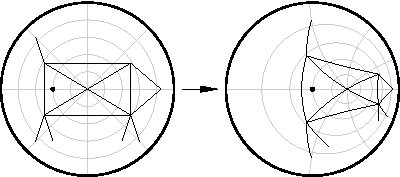
\includegraphics{figures/varphiplot}
\caption{Apa yang dilakukan $\varphi_a$ pada cakram satuan ketika $a=-0.4$.   Posisi $a$ dan $0=\varphi_a(a)$ ditandai dengan titik.%
\label{fig:varphiplot}}
\end{myfig}

\begin{prop}
Jika $f \in \Aut(\D)$, maka terdapat $a \in \D$
dan $\theta \in \R$ sedemikian sehingga
\begin{equation*}
f(z) = e^{i\theta} \frac{z-a}{1-\bar{a}z} = e^{i\theta} \varphi_a(z).
\end{equation*}
\end{prop}

\begin{proof}
Misalkan $b = f(0)$.
Perhatikan $g = \varphi_b \circ f$, yang merupakan suatu automorfisme,
dan $g(0) = 0$ karena
$\varphi_b(b) = 0$.
Seperti dalam bukti lema Schwarz, kita memperoleh fungsi holomorfik $h(z)$
sedemikian sehingga $g(z) = z h(z)$.  Berdasarkan
lema Schwarz, jika $z \in \D \setminus \{ 0 \}$, maka
\begin{equation*}
\sabs{h(z)} = \frac{\sabs{g(z)}}{\sabs{z}} \leq 1 .
\end{equation*}
Akibatnya, $h$ adalah pemetaan dari cakram ke cakram tertutup.

Namun, $h$ tidak dapat memiliki nol:
$h(z) = \frac{g(z)}{z}$ tidak dapat bernilai nol untuk $z \neq 0$ karena $g$ injektif
dan tidak dapat memiliki nol di $z=0$
karena $h(0) = \lim_{z\to 0} \frac{g(z)}{z} = g'(0) \neq 0$.  Karena $g$ adalah biholomorfisme, $g^{-1}$
kontinu. Jadi $g^{-1}(K)$ kompak untuk setiap himpunan kompak $K \subset \D$.
Dengan kata lain, $\sabs{g(z)}$ harus menuju $1$ ketika $z$
mendekati batas $\partial \D$ (latihan di bawah).
Maka $\sabs{h(z)}$ juga harus demikian.
Oleh karena itu, fungsi
$\sabs{h(z)}$ harus mencapai minimum di dalam $\D$, atau dengan kata
lain $\babs{\frac{1}{h(z)}}$ harus mencapai maksimum di dalam $\D$.  Jadi $h(z)$
adalah konstanta, dan $g(z) = \alpha z$ untuk suatu konstanta $\alpha$.
Jelas, 
$\sabs{\alpha} = 1$, sehingga $\alpha = e^{i\theta}$.  Dengan menerapkan
$\varphi_{-b}$ pada kedua ruas dari $e^{i\theta} z = \varphi_b \circ f$,
kita memperoleh
$f(z) = \varphi_{-b}(ze^{i\theta})
= e^{i \theta} \varphi_{-be^{-i\theta}}(z)$.
\end{proof}

\begin{exbox}
\begin{exercise}
Justifikasikan klaim dalam bukti tersebut.  Andaikan
$g \colon \D \to \D$ kontinu dan $g^{-1}(K)$ kompak
untuk setiap himpunan kompak $K \subset \D$.  Buktikan bahwa jika $\{ z_n \}$ adalah barisan
dalam $\D$ sedemikian sehingga $\sabs{z_n} \to 1$, maka
$\sabs{g(z_n)} \to 1$.
\end{exercise}

\begin{exercise}
Diberikan dua titik berbeda $a,b \in \D$, tunjukkan bahwa terdapat secara tunggal 
$f \in \Aut(\D)$
sedemikian sehingga $f(a) = b$ dan $f(b) = a$.
\end{exercise}

\begin{exercise}
Buktikan bahwa jika $\bH = \{ z \in \C : \Im z > 0 \}$ adalah setengah bidang atas
dan $f \colon \bH \to \bH$ adalah automorfisme dari $\bH$, maka
\begin{equation*}
f(z) = \frac{a z +b}{c z + d}
\avoidbreak
\end{equation*}
untuk bilangan real $a,b,c,d$ sedemikian sehingga $ad-bc > 0$.
\end{exercise}

\begin{exercise}
Andaikan $U \subset \C$ adalah domain, $\overline{\D} \subset U$,
dan $f \colon U \to \C$ holomorfik.
Andaikan $\sabs{f(z)}=1$ setiap kali $\sabs{z}=1$,
yakni, $f(\partial \D) \subset \partial \D$.
Temukan rumus untuk $f$.  Gunakan kerangka berikut:
\begin{exparts}
\item
Tunjukkan bahwa $f$ harus memiliki berhingga banyak nol dalam $\D$.  Artinya, $f(z) = 0$
untuk paling banyak berhingga banyak $z \in \D$.
\item
Andaikan $f$ tidak memiliki nol dalam $\D$.  Buktikan bahwa $f$ konstan
(dan tentukan jenis konstanta tersebut).
\item
Jika $f(a) = 0$, buktikan bahwa
$z \mapsto \frac{f(z)}{\varphi_a(z)}$ tetap holomorfik dalam $U$
(yakni, dapat didefinisikan di $a$ agar holomorfik dalam $U$)
dan tetap memetakan lingkaran ke lingkaran.
\item
Sekarang temukan rumus umum untuk $f$.
\end{exparts}
\end{exercise}

\begin{exercise}
Andaikan $f \colon \D \to \D$ adalah fungsi holomorfik dengan nol di
$n$ titik berbeda
$z_1,\ldots,z_n$, yakni, $f(z_\ell) = 0$ untuk $\ell=1,\ldots,n$.  Buktikan bahwa
\begin{equation*}
\sabs{f(z)} \leq \sabs{\varphi_{z_1}(z)  
\varphi_{z_2}(z)
\cdots
\varphi_{z_n}(z)} .
\end{equation*}
\end{exercise}

\begin{exercise} \label{exercise:schwarzpick}
Buktikan \emph{\myindex{lema Schwarz--Pick}}:
Jika $f \colon \D \to \D$ holomorfik, maka
\begin{equation*}
\abs{
\frac{f(z)-f(\zeta)}{1-\overline{f(\zeta)}f(z)}
}
\leq
\abs{
\frac{z-\zeta}{1-\widebar{\zeta}z} 
}
\qquad
\text{dan}
\qquad
\frac{\abs{f'(z)}}{1-\abs{f(z)}^2} \leq
\frac{1}{1-\abs{z}^2}
\end{equation*}
untuk semua $z,\zeta \in \D$.
Jika kesamaan berlaku dalam salah satu
pertidaksamaan untuk suatu $z \neq \zeta$,
maka $f$ adalah automorfisme dari $\D$.
Sebaliknya, jika $f$ adalah automorfisme dari $\D$,
maka kesamaan berlaku dalam kedua pertidaksamaan untuk
semua $z,\zeta \in \D$.
\end{exercise}
\end{exbox}

\pagebreak[0]
Secara khusus, lema Schwarz--Pick (\exerciseref{exercise:schwarzpick}) memberikan batas pada turunan
di semua titik.  Jika
$f \colon \D \to \D$ holomorfik, takkonstan, dan $f(a) = b$,
maka
\begin{equation*}
\sabs{f'(a)} \leq
\frac{1-\sabs{b}^2}{1-\sabs{a}^2} .
\end{equation*}
Jika kesamaan berlaku, maka $f(z) = \varphi_{-b}\bigl( e^{i\theta} \varphi_a(z)
\bigr)$ untuk suatu $\theta \in \R$.


%%%%%%%%%%%%%%%%%%%%%%%%%%%%%%%%%%%%%%%%%%%%%%%%%%%%%%%%%%%%%%%%%%%%%%%%%%%%%%
%%%%%%%%%%%%%%%%%%%%%%%%%%%%%%%%%%%%%%%%%%%%%%%%%%%%%%%%%%%%%%%%%%%%%%%%%%%%%%
%%%%%%%%%%%%%%%%%%%%%%%%%%%%%%%%%%%%%%%%%%%%%%%%%%%%%%%%%%%%%%%%%%%%%%%%%%%%%%

\chapter{Logaritma dan Cauchy} \label{ch:log}

\begin{myepigraph}
Jangan pernah meragukan keberanian orang Prancis. Merekalah yang menemukan bahwa siput dapat dimakan.

---Doug Larson
\end{myepigraph}

%%%%%%%%%%%%%%%%%%%%%%%%%%%%%%%%%%%%%%%%%%%%%%%%%%%%%%%%%%%%%%%%%%%%%%%%%%%%%%

\section{Logaritma dan bilangan lilit}
\label{sec:log}

\subsection{Logaritma}

Mari kita renungkan primitif dari $z^n$ untuk $n \in \Z$.\footnote{Tampaknya,
bukan, bahwa analisis kompleks elementer adalah kajian tentang $z^n$.}
Ketika $n \geq 0$, 
maka $z^n$ terdefinisi di seluruh bidang, dan suatu primitifnya hanyalah
$\frac{z^{n+1}}{n+1}$.  Jika $n < -1$, maka $z^n$ terdefinisi
di bidang berlubang $\C \setminus \{0\}$, dan sekali lagi
suatu primitifnya adalah $\frac{z^{n+1}}{n+1}$.  Bagaimana dengan $z^{-1} =
\nicefrac{1}{z}$?  Ia memiliki primitif, tetapi tidak pernah yang terdefinisi pada
seluruh bidang berlubang.

Kita telah menunjukkan bahwa pada setiap domain berbentuk bintang, suatu fungsi holomorfik memiliki
primitif.  Perhatikan apa yang disebut \emph{\myindex{bidang tersayat}}
\begin{equation*}
U = \C \setminus (-\infty,0] = \C \setminus \bigl\{ z \in \C : \Re z \leq 0 , \Im z = 0 \bigr\}.
\end{equation*}
Himpunan ini adalah domain berbentuk bintang dan
karena itu terdapat
primitif untuk $\nicefrac{1}{z}$ di $U$.
Jika kita
mensyaratkan bahwa primitif ini bernilai $0$ di $z=1$,
kita memperoleh suatu fungsi
\glsadd{not:Log}%
\begin{equation*}
\Log \colon U \to \C ,
\end{equation*}
yang disebut \emph{\myindex{cabang utama}} dari logaritma.
Sebelumnya kita melihat objek lain yang disebut \myquote{cabang utama,} 
yaitu cabang utama dari argumen, $\Arg$.  Mari kita tunjukkan bahwa
\begin{equation*}
\Log z = \log \sabs{z} + i \Arg z ,
\end{equation*}
dengan $\log \sabs{z}$ hanyalah logaritma real standar dari $\sabs{z}$.
Tetapkan $L(z) = \log \sabs{z} + i \Arg z$, dan mari kita tunjukkan bahwa $L = \Log$.
Kita memiliki $L(1) = 0 = \Log(1)$.  Sejauh ini baik.
Amati
\begin{equation*}
e^{L(z)}
=
e^{\log \sabs{z}} e^{i \Arg z}
=
\sabs{z} e^{i \Arg z} = z .
\end{equation*}
Jadi $L$ adalah invers dari fungsi eksponensial, setidaknya untuk $z \in U$.
Secara khusus, $L$ holomorfik berdasarkan teorema fungsi
invers.
Ambil turunan pada kedua ruas $z = e^{L(z)}$,
\begin{equation*}
1 = L'(z) e^{L(z)} = L'(z) z .
\end{equation*}
Dan jadilah!\footnote{Cauchy orang Prancis, bukan?}
Kita memiliki $L'(z) = \nicefrac{1}{z}$, sehingga $L = \Log$.

Jika kita menggunakan cabang argumen yang berbeda, kita memperoleh
antiturunan lain dari $\nicefrac{1}{z}$.  Kita 
membuat definisi
\glsadd{not:log}%
\begin{equation*}
\log z \overset{\text{def}}{=} \log \sabs{z} + i \arg z .
\end{equation*}
Pada pandangan pertama, definisi ini benar-benar ganjil.  Pertama, $\log$ di
ruas kiri adalah $\log$ yang berbeda dari $\log$ di ruas kanan.  Di ruas kanan, ia adalah
$\log$ real standar, yakni, $\log \colon (0,\infty) \to \R$,
dengan $\log 1 = 0$.
Namun, $\log$ di ruas kiri
bahkan bukan sebuah fungsi; ia memiliki takhingga banyak nilai untuk setiap $z$,
karena $\arg$ di ruas kanan memiliki takhingga banyak nilai.
Nilai $\log (-1)$ adalah $\pi i$, tetapi juga $-\pi i$, $3\pi i$,
atau $(\pi + 2\pi k)i$ untuk sembarang $k \in \Z$.  Jadi $\log$ adalah fungsi persis sejauh
$\arg$ adalah fungsi.  Lihat \figureref{fig:loggraph}.
Peran ganda \myquote{$\log$} hampir tidak pernah menjadi
masalah dan biasanya jelas $\log$ mana yang dimaksud berdasarkan
jenis objek yang dimasukkan ke dalamnya.


\begin{myfig}
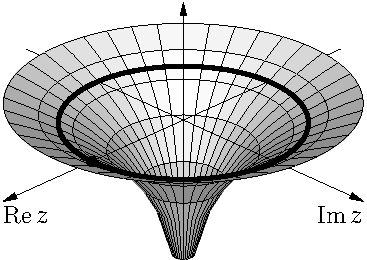
\includegraphics{figures/logrealgraph}
\qquad
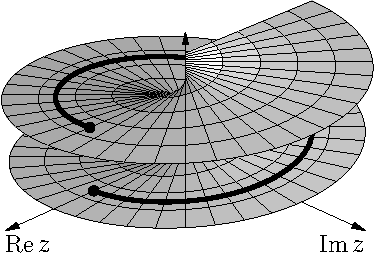
\includegraphics{figures/arggraph2}
\caption{\myquote{Grafik} bagian real (kiri) dan bagian imajiner (kanan)
dari logaritma kompleks $\log z = \log \sabs{z} + i \arg z$.  Bagian imajiner
merupakan spiral takhingga, tetapi hanya dua putaran yang digambarkan.  Suatu lintasan pada
grafik di sepanjang lingkaran satuan ditandai.\label{fig:loggraph}}
\end{myfig}

Walaupun $\log$ sebenarnya bukan fungsi---ia adalah fungsi
bernilai jamak\footnote{%
Cauchy: Betapa malangnya!  Aku benci logaritma! Aku ingin menjadi tukang leding.}---inilah
definisi yang kita inginkan.
Cabang utama,
yang berguna ketika seseorang ingin memperoleh sejumlah nilai aktual, sering kali bukan yang kita
perlukan; kegunaannya tidak sebesar yang mungkin dibayangkan.
Dan berhati-hatilah bahwa komputer suka memberikan kembali cabang utama bahkan 
ketika hal itu tidak masuk akal.

Jadi bagaimana kita menggunakan $\log$?  Ia muncul dalam integral garis, yang digunakan
untuk menghitung dan mengklasifikasikan nol (akar) dan/atau singularitas fungsi, atau
sebaliknya---nol dan singularitas digunakan untuk menghitung integral garis.
Mari kita hitung integral $\nicefrac{1}{z}$ mengelilingi lingkaran
satuan $\partial \D$, yang seperti biasa berorientasi berlawanan arah jarum jam (diparameterkan
oleh $e^{it}$).  Andaikan kita memulai dan mengakhiri pengintegralan di 
$z=1$:
\begin{equation*}
\int_{\partial \D} \frac{1}{z} \, dz
= \log 1 - \log 1 = 2\pi i.
\end{equation*}
Itu tidak masuk akal, bukan?  Nah, sebenarnya ini hanya boleh dilakukan
dengan tanda kutip:
\begin{equation*}
\int_{\partial \D} \frac{1}{z} \, dz
\enspace
\text{``$=$''}
\enspace
\log 1 - \log 1
\enspace
\text{``$=$''}
\enspace
2\pi i.
\end{equation*}
Itu jauh lebih baik,
bukan?\footnote{Tidak! Sekarang aku juga ingin menjadi tukang leding!}
Kesamaan-kesamaan tersebut hanya benar secara moral.
Jika ditafsirkan dengan tepat, persis itulah yang terjadi.  Anda benar-benar mengurangkan
salah satu nilai $\log 1$ dari nilai lain $\log 1$.  Untuk menentukan
nilai mana dikurangkan dari nilai mana, mulailah dengan, katakanlah, $\log 1 = 0$, dan ikuti
fungsi tersebut perlahan-lahan di sepanjang lingkaran serta perhatikan bahwa $i \arg z$ bertambah dari $0$ hingga
$2\pi i$.  Jadi, $\log 1$ di akhir adalah $2 \pi i$.  Lihat lintasan
yang ditandai pada \figureref{fig:loggraph}; lompatan pada bagian imajiner antara
awal dan akhir tepat sebesar $2\pi i$ itu.

Untuk mempermudah bekerja dengan $\log$, biasanya kita membicarakan suatu
\emph{\myindex{cabang logaritma}}.  Jadi, $L \colon U \to \C$ adalah cabang
logaritma jika $L$ holomorfik, $L'(z) = \nicefrac{1}{z}$, dan $L(z)$ sama
dengan suatu nilai $\log z$ untuk setiap $z \in U$.  Tidak mungkin mendefinisikan
cabang logaritma pada setiap $U$, tetapi, misalnya, kita dapat melakukannya pada setiap
$U$ berbentuk bintang dengan $0 \notin U$.  Secara umum, kita dapat mendefinisikan cabang
logaritma pada setiap domain terhubung sederhana, yakni, domain tanpa lubang,
yang tidak memuat nol.
Lebih lanjut tentang hal itu nanti.  Demikian pula, kita mendefinisikan cabang-cabang $\log (z-p)$,
suatu primitif dari $\frac{1}{z-p}$, dan dalam hal ini domainnya
tidak boleh memuat $p$.

Kita juga dapat membicarakan cabang secara lebih longgar, dan membicarakan
mengikuti cabang tersebut di sepanjang suatu lintasan.  Kita tidak mendefinisikan
satu cabang tunggal---kita mendefinisikan cabang pada suatu himpunan terbuka kecil,
mengikuti nilainya untuk beberapa waktu, lalu beralih ke cabang lain yang 
kebetulan sama dengan cabang pertama pada titik tempat kita
beralih.  Lihat \figureref{fig:followbranch}.  Sesungguhnya, tepat itulah yang kita lakukan dalam
\myquote{perhitungan} di atas: Kita mengikuti $\log$ dari $1$ di sepanjang lingkaran hingga kita
kembali ke $1$, dan cabang-cabang yang kita ikuti berakhir dengan selisih $2\pi i$.
Sebentar lagi kita akan melihat prosedur ini digunakan secara lebih formal.

%Used in two places
\begin{myfig}
\subimport*{figures/}{followbranch.pdf_t}
\caption{Mengikuti suatu cabang.
Cabang-cabang tersebut didefinisikan dalam cakram-cakram
(tidak harus berupa cakram).
Titik-titik tempat cabang-cabang itu seharusnya sama
ditandai.\label{fig:followbranch}}
\end{myfig}

\begin{exbox}
\begin{exercise}
Andaikan $a \in \C \setminus \{ 0 \}$, dan
$R_a = \{ \lambda a \in \C : \lambda \geq 0 \}$
adalah sinar dari titik asal yang melalui $a$.  Buktikan
bahwa terdapat cabang dari $\log$ pada $\C \setminus R_a$.
\end{exercise}

\begin{exercise}
Untuk $n \in \N$, misalkan $\gamma \colon [0,2\pi] \to \C$ diberikan oleh $\gamma(t) = e^{int}$,
yaitu lingkaran satuan yang dilalui $n$ kali berlawanan arah jarum jam.  Hitung
$\int_\gamma \frac{1}{z} \, dz$.  Berikan argumen dengan memecah integral
menjadi beberapa bagian dan menggunakan cabang-cabang dari $\log$.
\end{exercise}

\begin{exercise}
Andaikan
$U \subset \C$ terbuka dengan
$\partial \D \subset U$,
$f \colon U \to \C$ holomorfik,
sedemikian sehingga
$f(z)$ tidak pernah berupa bilangan real negatif ataupun nol.
Hitung
$\int_{\partial \D} \frac{f'(z)}{f(z)} \, dz$.
\end{exercise}

\begin{exercise}
Andaikan $\gamma \colon [a,b] \to \C \setminus \{ 0 \}$ adalah lintasan $C^1$ sepotong-sepotong
sedemikian sehingga $\gamma(a) = \gamma(b) = -1$, tetapi $\gamma(t)$ tidak pernah
berupa bilangan real negatif untuk setiap $t \in (a,b)$.  Dengan menggunakan cabang utama dari
$\log$, buktikan bahwa
\begin{equation*}
\int_\gamma \frac{1}{z} \, dz = -2\pi i, 0, \text{ atau } 2\pi i.
\avoidbreak
\end{equation*}
Temukan secara eksplisit
tiga $\gamma$ yang masing-masing menghasilkan salah satu dari ketiga kemungkinan ini.
\end{exercise}
\end{exbox}

\subsection{Bilangan lilit}

Baiklah.  Mari kita buat lebih rigor.

\begin{defn}\label{defn:windingnumber}
Misalkan $\Gamma$ adalah
suatu siklus,
dan $p \notin \Gamma$.  Maka
\glsadd{not:windnum}%
\begin{equation*}
n(\Gamma;p)
\overset{\text{def}}{=}
\frac{1}{2\pi i} \int_\Gamma \frac{1}{z-p} \, dz
\end{equation*}
disebut
\emph{\myindex{bilangan lilit}} dari $\Gamma$ mengelilingi $p$, atau
\emph{\myindex{indeks}} dari $\Gamma$ terhadap $p$.
\end{defn}

Secara intuitif, bilangan lilit adalah banyaknya kali $\Gamma$ melilit
$p$, berlawanan arah jarum jam.  Intuisi ini dikonfirmasi dengan mengintegralkan
$\nicefrac{1}{z}$ untuk lintasan $e^{it}$ dengan $t \in [0,2\pi]$ sehingga diperoleh
bilangan lilit $1$ mengelilingi $p=0$,
karena lintasan itu mengelilingi nol satu kali berlawanan arah jarum jam.  Jika kita melakukan
integral dengan $e^{2it}$, kita mengelilingi nol dua kali 
berlawanan arah jarum jam, dan bilangan lilitnya benar-benar $2$.  Demikian pula,
jika kita menggunakan $e^{-it}$, kita mengelilingi nol satu kali dalam
arah jarum jam, dan bilangan lilitnya adalah $-1$.

Hal pertama yang perlu diamati adalah bahwa bilangan lilit merupakan bilangan bulat.

\begin{prop} \label{prop:indexinteger}
Andaikan $\Gamma$ adalah suatu siklus dan $p \notin \Gamma$.  Maka
$n(\Gamma;p)$ adalah bilangan bulat.
\end{prop}

Buktinya adalah dengan mengambil suatu lintasan tertutup $\gamma$
dan mengikuti cabang $\log$ sepanjang $\gamma$, lalu
melihat seberapa besar perubahannya.  Lihat \figureref{fig:followbranch}, tempat kita
berjalan mengelilingi satu gelung penuh.  Karena kita mengikuti argumen
dan berjalan beberapa kali mengelilingi $p$ sepanjang $\gamma$,
argumen berubah sebesar suatu kelipatan bilangan bulat dari $2\pi$.

\begin{proof}
Suatu siklus (ekuivalen dengan) kombinasi linear (atas bilangan bulat) dari lintasan-lintasan tertutup,
jadi kita hanya perlu memperhatikan lintasan $C^1$ sepotong-sepotong yang tertutup.
Misalkan $\gamma \colon [0,1] \to \C$ adalah lintasan tersebut.
Lintasan $\gamma$ sebagai himpunan adalah kompak.  Ia dapat ditutupi oleh berhingga banyak
cakram $D_1,\ldots,D_n$, yang tidak satu pun memuat $p$, dan sedemikian sehingga terdapat
partisi $0 = t_0 < t_1 < t_2 < \cdots < t_n = 1$ dengan
$\gamma\bigl([t_{j-1},t_j]\bigr) \subset D_j$.  Setiap $D_j$ berbentuk bintang dan
tidak memuat $p$,
sehingga pada masing-masing cakram itu terdapat cabang dari $\log (z-p)$.  Sebut cabang itu $L_j$.
Pilih $L_1$ secara sembarang, lalu pilih $L_2,\ldots,L_n$ secara berurutan
sedemikian sehingga
$L_j\bigl(\gamma(t_j)\bigr) = L_{j+1}\bigl(\gamma(t_j)\bigr)$.
Sebut $z_0 = \gamma(0) = \gamma(1)$.  Maka
\begin{multline*}
n(\gamma;p)
=
\frac{1}{2\pi i} \int_\gamma \frac{1}{z-p} \, dz
=
\frac{1}{2\pi i} \int_0^1 \frac{\gamma'(t)}{\gamma(t)-p} \, dt
=
\frac{1}{2\pi i} \sum_{j=1}^n \int_{t_{j-1}}^{t_j} \frac{\gamma'(t)}{\gamma(t)-p} \, dt
\\
=
\frac{1}{2\pi i} \sum_{j=1}^n
\Bigl(
L_j\bigl(\gamma(t_j)\bigr) -
L_j\bigl(\gamma(t_{j-1})\bigr)
\Bigr)
=
\frac{1}{2\pi i} \bigl( L_n(z_0) - L_1(z_0) \bigr) .
\end{multline*}
Karena $L_n$ dan $L_1$ keduanya merupakan cabang dari $\log(z-p)$, selisih keduanya adalah
$2\pi k i$ untuk suatu $k \in \Z$, sebab masing-masing berbentuk
$\log\sabs{z_0-p} + i \arg (z_0-p)$ untuk suatu nilai dari
$\arg$.
\end{proof}

\begin{exbox}
\begin{exercise}
Lengkapi perincian tentang keberadaan partisi tersebut.  Artinya, setelah Anda
menutupi $\gamma$ dengan berhingga banyak cakram yang tidak memuat $p$, tunjukkan bahwa
partisi $t_0,\ldots,t_n$ ada.  Petunjuk: Beberapa cakram mungkin
\myquote{berulang,} tetapi pastikan bahwa Anda tidak \myquote{terhenti}
sebelum mencapai $1$.
\end{exercise}
\end{exbox}

Hal kedua yang perlu diamati adalah bahwa $n(\Gamma;z)$ konstan selama kita
tidak melintasi $\Gamma$.

\begin{prop} \label{prop:windingconstant}
Diberikan suatu siklus $\Gamma$,
fungsi $z \mapsto n(\Gamma;z)$ konstan pada
komponen topologis dari $\C \setminus \Gamma$.
Lebih lanjut, $n(\Gamma;z) = 0$ untuk $z$ pada komponen takterbatas
dari $\C \setminus \Gamma$.
\end{prop}

Karena $\Gamma$ kompak, harus terdapat satu komponen takterbatas yang tunggal
dari komplemen $\C \setminus \Gamma$, dan mungkin beberapa komponen
terbatas.
Lihat \figureref{fig:indexconstant} sebagai contoh.

\begin{myfig}
\subimport*{figures/}{indexconstant.pdf_t}
\caption{Komponen-komponen dari $\C \setminus \Gamma$ dengan 
bilangan lilit mengelilingi titik-titik dalam komponen tersebut
ditandai.\label{fig:indexconstant}}
\end{myfig}

\begin{proof}
Mari kita tunjukkan bahwa fungsi
\begin{equation*}
p \mapsto n(\Gamma;p) = \frac{1}{2\pi i} \int_\Gamma \frac{1}{z-p} \, dz
\end{equation*}
kontinu pada $\C \setminus \Gamma$.
Tetapkan $p_0 \in \C \setminus \Gamma$, dan misalkan
\glsadd{not:distancetoset}%
$d = d(p_0,\Gamma)$ adalah
jarak dari 
$p_0$ ke $\Gamma$, yakni
$d = \inf \bigl\{ \sabs{z-p_0} : z \in \Gamma \bigr\}$.
Karena $\Gamma$ kompak, $d > 0$.  
Untuk setiap $p \in \Delta_{d/2}(p_0)$, kita memiliki $\sabs{z-p} \geq
\nicefrac{d}{2}$ untuk setiap $z \in \Gamma$.  Misalkan $\ell$ adalah panjang
$\Gamma$, yakni, $\ell = \int_\Gamma \sabs{dz}$.  Maka
\begin{equation*}
\begin{split}
\abs{n(\Gamma;p_0)-n(\Gamma;p)}
=
\abs{\frac{1}{2\pi i} \int_\Gamma \frac{p_0-p}{(z-p_0)(z-p)} \, dz}
& \leq
\frac{1}{2\pi} \int_\Gamma \frac{\sabs{p_0-p}}{\sabs{z-p_0}\sabs{z-p}} \, \sabs{dz}
\\
& \leq 
\frac{\ell}{\pi {d}^2} \sabs{p_0-p} .
\end{split}
\end{equation*}
Jadi, $n(\Gamma;p)$ adalah fungsi kontinu dari $p$.
Karena kontinu
dan bernilai bilangan bulat, fungsi ini konstan pada setiap komponen terhubung dari
$\C \setminus \Gamma$ (himpunan tempat fungsi itu terdefinisi).

Untuk setiap $p \in \C \setminus \Gamma$,
\begin{equation*}
\sabs{n(\Gamma;p)} \leq \frac{1}{2\pi} \int_\Gamma \frac{1}{\sabs{z-p}} \,
\sabs{dz} \leq \frac{1}{2\pi} \frac{\ell}{d(p,\Gamma)} .
\end{equation*}
Pada komponen takterbatas---karena $\Gamma$ kompak---terdapat $p$
dengan $d(p,\Gamma)$ sebesar apa pun, sehingga $n(\Gamma;p)$ sekecil apa pun
pada komponen ini.  Karena konstan, nilainya nol.
\end{proof}

\begin{exbox}
\begin{exercise}%[\neededexmark]
\label{exercise:windingcircle}
Tunjukkan bahwa $n\bigl(\partial \Delta_r(p);z\bigr) = 0$ jika $z \notin
\overline{\Delta_r(p)}$ dan 
$n\bigl(\partial \Delta_r(p);z\bigr) = 1$ jika $z \in \Delta_r(p)$.
\end{exercise}

\begin{exercise}
Misalkan $n \in \Z$.  Lintasan $\gamma \colon [0,2\pi] \to \C$, dengan
$\gamma(t) = p + re^{in t}$, berjalan $n$ kali
berlawanan arah jarum jam mengelilingi $\partial \Delta_r(p)$.
Buktikan bahwa
$n\bigl(\gamma;z\bigr) = n$ jika $z \in \Delta_r(p)$.
\end{exercise}

\begin{exercise}%[\neededexmark]
\label{exercise:windingcircles}
Andaikan $0 < r_1 < r_2 < \infty$.
Misalkan $\Gamma = \partial \Delta_{r_2}(p) - \partial \Delta_{r_1} (p)$
(yakni, lingkaran luar berjalan berlawanan arah jarum jam, sedangkan lingkaran dalam berjalan
searah jarum jam).
Buktikan bahwa jika $z \in \C$ sedemikian sehingga $\sabs{z-p} < r_1$, maka
$n(\Gamma;z) = 0$.  Jika $r_1 < \sabs{z-p} < r_2$, maka
$n(\Gamma;z) = 1$.  Jika $r_2 < \sabs{z-p}$, maka
$n(\Gamma;z) = 0$.
\end{exercise}

\begin{exercise}%[\optneededexmark]
\label{exercise:rayktimes}
Andaikan $\gamma \colon [a,b] \to \C$ adalah lintasan $C^1$ tertutup sedemikian sehingga
$\gamma(a) = \gamma(b)$ adalah suatu bilangan real negatif.  Andaikan
bahwa $\gamma(t)$ real dan negatif hanya untuk $k$ nilai $t$ yang berbeda (yang
mencakup $t=a$ dan $t=b$, sehingga $k \geq 2$), dan setiap kali $\gamma(t)$ real dan negatif,
berlaku $\Im \gamma'(t) < 0$.  Buktikan bahwa $n(\gamma;0) = k-1$.  Petunjuk: Gunakan
cabang utama.
\end{exercise}
\end{exbox}


%%%%%%%%%%%%%%%%%%%%%%%%%%%%%%%%%%%%%%%%%%%%%%%%%%%%%%%%%%%%%%%%%%%%%%%%%%%%%%

\section{Versi homologi dari teorema Cauchy}

\begin{defn}
Misalkan $U \subset \C$ terbuka dan $\Gamma$
suatu siklus
dalam $U$
sedemikian sehingga $n(\Gamma;p) = 0$ untuk semua $p \in \C \setminus U$.
Kita kemudian
mengatakan bahwa $\Gamma$ \emph{\myindex{homolog dengan nol} dalam $U$}.
\end{defn}

Makna homolog dengan nol adalah bahwa $\Gamma$ tidak melilit sembarang
titik dalam komplemen $U$.
Perhatikan bahwa \myquote{homolog dengan nol} tidak berarti
\myquote{ekuivalen dengan nol.}
Sebagai contoh, jika $U = \C$, maka setiap $\Gamma$ secara trivial homolog dengan nol.
Perhatikan pula ketergantungannya pada $U$.  Lingkaran satuan homolog dengan nol dalam
$U = \C$, tetapi tidak homolog dengan nol dalam $U = \C \setminus \{ 0 \}$.

\begin{thm}[Rumus integral Cauchy (versi homologi)]
\index{rumus integral Cauchy!homologi}
\label{thm:CIFhomology}
Andaikan $U \subset \C$ terbuka, $f \colon U \to \C$ holomorfik, dan
$\Gamma$ adalah
suatu siklus
dalam $U$
yang homolog dengan nol dalam $U$.
Maka untuk $z \in U \setminus \Gamma$,
\begin{equation*}
n(\Gamma;z)
f(z)
=
\frac{1}{2\pi i}
\int_{\Gamma}
\frac{f(\zeta)}{\zeta-z}
\,
d \zeta .
\end{equation*}
\end{thm}

Dalam buktinya\footnote{%
Bukti elegan ini relatif baru, dari tahun 1971, berkat John Dixon.},
dengan cara yang agak aneh, kita akan mengambil selisih kedua
ruas persamaan tersebut dan memperluasnya menjadi fungsi entire
(meskipun $U$ mungkin kecil).  Kemudian kita akan menggunakan
teorema Liouville (\thmref{thm:Liouville}) untuk menunjukkan bahwa selisih ini
nol.

\begin{proof}
Definisikan $g \colon U \times U \to \C$ dengan
\begin{equation*}
g(\zeta,z) =
\begin{cases}
\frac{f(\zeta)-f(z)}{\zeta-z} & \text{jika } \zeta \neq z , \\
f'(\zeta)                 & \text{jika } \zeta = z .
\end{cases}
\end{equation*}

\begin{exbox}
\begin{exercise}
Buktikan bahwa $g(\zeta,z)$ kontinu dalam $U \times U$, dan bahwa
fungsi $z \mapsto g(\zeta,z)$ holomorfik untuk setiap $\zeta \in U$ yang tetap.
Petunjuk: Satu-satunya bagian taktrivial dari bukti ini adalah menunjukkan bahwa $z \mapsto
g(\zeta,z)$
holomorfik di $z=\zeta$.
\end{exercise}
\end{exbox}

Misalkan
\begin{equation}\label{eq:CIFdefofh}
h(z) = 
\begin{cases}
\int_\Gamma g(\zeta,z) \, d\zeta & \text{jika } z \in U , \\
\int_\Gamma \frac{f(\zeta)}{\zeta-z} \, d\zeta & \text{jika } z \not \in
\Gamma \text{ dan } n(\Gamma;z) = 0 .
\end{cases}
\end{equation}
Karena $n(\Gamma;z) = 0$ untuk semua $z \in \C \setminus U$
($\Gamma$ homolog dengan nol),
fungsi $h(z)$ terdefinisi untuk setiap $z \in \C$.
Sayangnya, di beberapa titik
kita memiliki dua definisi.
Untuk menunjukkan bahwa $h(z)$ terdefinisi dengan baik, kita harus menunjukkan bahwa jika
$z \in U \setminus \Gamma$ dan
$n(\Gamma;z) = 0$, maka kedua definisi tersebut bersepakat.
Perhatikan suatu $z$ demikian (khususnya, $z \notin \Gamma$).  Maka,
\begin{equation*}
\int_\Gamma g(\zeta,z) \, d\zeta
=
\int_\Gamma \frac{f(\zeta)-f(z)}{\zeta-z} \, d\zeta
=
\int_\Gamma \frac{f(\zeta)}{\zeta-z} \, d\zeta
-
f(z) (2\pi i) n(\Gamma;z)
=
\int_\Gamma \frac{f(\zeta)}{\zeta-z} \, d\zeta .
\end{equation*}
Jadi, $h \colon \C \to \C$ terdefinisi dengan baik.

Selanjutnya, kita tunjukkan bahwa $h$
holomorfik.
Sifat holomorfik adalah sifat lokal, jadi kita hanya perlu membuktikannya 
pada suatu lingkungan dari setiap titik.
Himpunan tempat $n(\Gamma;z) = 0$ adalah terbuka karena merupakan
gabungan beberapa komponen topologis dari $\C \setminus \Gamma$.
Jadi, setiap titik di $\C$ memiliki suatu lingkungan tempat $h$ didefinisikan
sepenuhnya oleh salah satu ekspresi dalam \eqref{eq:CIFdefofh}.
Diberikan sembarang titik di $\C$,
ambil lingkungan tempat salah satu ekspresi mendefinisikan
$h$ dan terapkan \corref{cor:holfuncbyintegral}.

Komponen takterbatas dari $\C \setminus \Gamma$ termuat dalam
himpunan tempat $n(\Gamma;z) = 0$, sehingga pada komponen ini, $h$ didefinisikan oleh
ekspresi kedua.  Perhatikan suatu $z$ dalam komponen ini.
Andaikan $\sabs{f(\zeta)} \leq M$ untuk $\zeta \in \Gamma$, misalkan $\ell$ adalah panjang
$\Gamma$, dan misalkan $d(z,\Gamma)$ adalah jarak dari $z$ ke $\Gamma$.  Maka
\begin{equation*}
\sabs{h(z)}
=
\abs{
\int_\Gamma \frac{f(\zeta)}{\zeta-z} \, d\zeta
}
\leq
\int_\Gamma \abs{\frac{f(\zeta)}{\zeta-z}} \, \sabs{d\zeta}
\leq
\frac{M \ell}{d(z,\Gamma)} .
\end{equation*}
Ketika $z \to \infty$, demikian pula $d(z,\Gamma) \to \infty$, sehingga $h(z) \to 0$.
Secara khusus, $h$ adalah fungsi entire terbatas dan
teorema Liouville menyatakan bahwa $h$ konstan. Selain itu, konstanta tersebut harus nol.
Jadi, andaikan $z \in U \setminus \Gamma$.  Maka
\begin{equation*}
0 = h(z) =
\int_\Gamma \frac{f(\zeta)-f(z)}{\zeta-z} \, d\zeta
=
\int_\Gamma \frac{f(\zeta)}{\zeta-z} \, d\zeta
-
f(z) (2\pi i) n(\Gamma;z) . \qedhere
\end{equation*}
\end{proof}

Teorema Cauchy segera mengikuti dari rumus integral tersebut.
Bahkan, kedua teorema tersebut ekuivalen; lihat latihan.

\begin{thm}[Teorema Cauchy (versi homologi)]
\index{teorema Cauchy!homologi}%
\label{thm:CThomology}%
Andaikan $U \subset \C$ terbuka,
$f \colon U \to \C$ holomorfik,
dan $\Gamma$ adalah
suatu siklus
dalam $U$.
Jika $\Gamma$
homolog dengan nol dalam $U$,
maka
\begin{equation*}
\int_\Gamma f(z) \, dz = 0 .
\end{equation*}
\end{thm}

\begin{proof}
Tetapkan $z \in U \setminus \Gamma$.  Terapkan 
rumus integral Cauchy pada fungsi $\zeta \mapsto
(\zeta-z)f(\zeta)$ di $\zeta=z$:
\begin{equation*}
0 = n(\Gamma;z) (z-z)f(z) =
\frac{1}{2\pi i} \int_\Gamma \frac{(\zeta-z)f(\zeta)}{\zeta-z} \, d\zeta
=
\frac{1}{2\pi i} \int_\Gamma f(\zeta) \, d\zeta . \qedhere
\end{equation*}
\end{proof}

\begin{defn}
Dua siklus
$\Gamma_0$ dan $\Gamma_1$ dalam $U
\subset \C$ dikatakan \emph{\myindex{homolog}} dalam $U$
jika $n(\Gamma_0;p) = n(\Gamma_1;p)$ untuk semua $p \in \C \setminus U$.
\end{defn}

Secara ekuivalen, $\Gamma_0$ dan $\Gamma_1$ homolog dalam $U$ jika
$n(\Gamma_0 - \Gamma_1;p) = 0$ untuk semua $p \in \C \setminus U$,
yakni, $\Gamma_0-\Gamma_1$ homolog dengan nol dalam $U$.

\begin{cor} \label{cor:homologoussameint}
Misalkan $U \subset \C$ terbuka dan $f \colon U \to \C$ holomorfik,
dan misalkan
$\Gamma_0$ dan $\Gamma_1$ adalah siklus dalam $U$.
Jika 
$\Gamma_0$ dan $\Gamma_1$
homolog dalam $U$, maka
\begin{equation*}
\int_{\Gamma_0} f(z)\, dz = 
\int_{\Gamma_1} f(z)\, dz .
\end{equation*}
\end{cor}

Buktinya langsung dengan menerapkan teorema Cauchy pada $\Gamma_0-\Gamma_1$.

\begin{exbox}
\begin{exercise}[Mudah]
Andaikan $\Gamma$ adalah suatu siklus sedemikian sehingga
$0 \notin \Gamma$ dan
$n(\Gamma;0) = k$.  Hitung
\begin{equation*}
\int_{\Gamma} \frac{\cos z}{z} \, dz .
\end{equation*}
\end{exercise}

\begin{exercise}
Misalkan $\Gamma$ adalah
suatu siklus dalam $\C \setminus \{ 0 \}$.
Buktikan bahwa $\Gamma$ homolog dalam $\C \setminus \{ 0 \}$
dengan $n \partial \D$ untuk suatu $n \in \Z$.
\end{exercise}

\begin{exercise} \label{exercise:H1U}
\begin{exparts}
\item
Tunjukkan bahwa relasi homolog dalam $U$ adalah relasi ekuivalensi pada siklus.
\item
Buktikan bahwa penjumlahan siklus membuat himpunan kelas ekuivalensi
menjadi suatu grup abelian, yaitu
\emph{\myindex{grup homologi pertama}}\index{grup homologi pertama} dari $U$,
yang biasanya ditulis $H_1(U)$.
\item
Hitung $H_1(\C \setminus \{ 0 \})$ (yakni,
tentukan grup yang isomorfik dengannya).
\end{exparts}
\end{exercise}

\begin{exercise}
Buktikan bahwa kedua teorema tersebut
(versi homologi dari teorema Cauchy dan rumus integral Cauchy)
ekuivalen secara logis, yakni, yang satu mengikuti
dari yang lain.  Kita telah membuktikan bahwa rumus integral Cauchy
mengakibatkan teorema Cauchy.  Jadi buktikan bahwa
teorema Cauchy mengakibatkan rumus integral Cauchy.
\end{exercise}

\begin{exercise}
Misalkan $U \subset \C$ terbuka dan $\Gamma$ suatu siklus dalam $U$
yang homolog dengan nol dalam $U$.
Andaikan $n(\Gamma;z_1) = k_1$ dan $n(\Gamma;z_2) = k_2$ untuk
dua titik berbeda $z_1,z_2 \in U \setminus \Gamma$.
Misalkan $f \colon U \setminus \{z_1,z_2\} \to \C$
holomorfik.
Andaikan $0< \epsilon < \sabs{z_1-z_2}$ cukup kecil sehingga
$\overline{\Delta_\epsilon(z_j)} \subset U$ untuk $j=1,2$,
dan bahwa
$\int_{\partial \Delta_\epsilon(z_1)} f(z) \, dz = A$ dan 
$\int_{\partial \Delta_\epsilon(z_2)} f(z) \, dz = B$.
Dalam hubungannya dengan $k_1$, $k_2$, $A$, dan $B$,
hitung
\begin{equation*}
\int_{\Gamma} f(z) \, dz .
\end{equation*}
\end{exercise}
\end{exbox}


%%%%%%%%%%%%%%%%%%%%%%%%%%%%%%%%%%%%%%%%%%%%%%%%%%%%%%%%%%%%%%%%%%%%%%%%%%%%%%

\section{Domain terhubung sederhana}

Secara kasar, domain terhubung sederhana\footnote{%
Tidak ada kesepakatan di antara berbagai matematikawan (saya telah bertanya kepada beberapa orang) mengenai apakah
suatu himpunan yang tidak terhubung (oleh lintasan) dapat disebut \myquote{terhubung sederhana.}
Untuk menghindari perdebatan sengit dengan berbagai jenis topolog,
sebaiknya istilah tersebut tidak didefinisikan untuk himpunan takterhubung.
Oleh karena itu, kita mendefinisikannya hanya untuk domain.}
adalah domain tanpa lubang.  Pernyataan berikut
mungkin bukan definisi standar, tetapi untuk domain dalam $\C$
(himpunan terbuka terhubung),
definisi ini ekuivalen dengan definisi yang benar.
Kita akan mendefinisikan istilah tersebut dengan tepat setelah sampai pada
homotopi.\footnote{Homotopi berada dalam bagian opsional, dan itulah
alasan kita membuat definisi \myquote{keliru} ini.}
Kadang-kadang kita dapat mengatakan
\myquote{terhubung sederhana dalam arti homologi}
untuk menekankan bahwa kita menggunakan definisi khusus ini.

\begin{defn} \label{defn:simplyconnected:homology}
Suatu domain $U \subset \C$ disebut \emph{terhubung sederhana}%
\index{terhubung sederhana!dalam arti homologi}
jika setiap siklus dalam $U$
homolog dengan nol dalam $U$.
\end{defn}

Dengan kata lain, $U$ terhubung sederhana
jika $n(\Gamma;p) = 0$ untuk setiap siklus $\Gamma$ dalam $U$ dan
setiap $p \in \C \setminus U$.
Jadi, dalam domain terhubung sederhana, tidak ada siklus dalam $U$ yang dapat melilit sembarang titik
dari $\C \setminus U$.  Contoh domain terhubung sederhana adalah $\C$, $\D$, atau
$\bH$.  Contoh domain yang tidak terhubung sederhana adalah
$\C \setminus \{ 0 \}$.
Lihat latihan di bawah.


\begin{exbox}
\begin{exercise}
\begin{exparts}
\item
Buktikan bahwa setiap domain berbentuk bintang (misalnya, $\C$, $\D$, dan $\bH$) dalam $\C$ terhubung sederhana.
\item
Buktikan bahwa $\C \setminus \{ 0 \}$ tidak terhubung sederhana.
\end{exparts}
\end{exercise}

\begin{exercise}
Buktikan bahwa jika $U \subset \C$ biholomorfik dengan $\D$, maka $U$
terhubung sederhana.
\end{exercise}

\begin{exercise}
Buktikan bahwa suatu domain $U \subset \C$ terhubung sederhana jika dan hanya jika
grup homologi pertama
$H_1(U)$ isomorfik dengan grup trivial $\{ 0 \}$.
Lihat \exerciseref{exercise:H1U}.
\end{exercise}
\end{exbox}

Suatu kasus khusus (tetapi umum) dari versi homologi teorema Cauchy,
\thmref{thm:CThomology}, dapat dinyatakan sebagai kasus terhubung sederhana dari teorema Cauchy.

\begin{thm}[Teorema Cauchy (versi terhubung sederhana)]
\index{teorema Cauchy!terhubung sederhana}%
Misalkan $U \subset \C$ adalah domain terhubung sederhana dan $f \colon U \to \C$
holomorfik.  Jika $\Gamma$ adalah suatu siklus dalam $U$, maka
\begin{equation*}
\int_\Gamma f(z) \, dz = 0 .
\end{equation*}
\end{thm}

Bukti langsung mengikuti dari \thmref{thm:CThomology},
karena jika $U$ terhubung sederhana, maka
setiap $\Gamma$ dalam $U$ homolog dengan nol dalam $U$.
Dalam domain terhubung sederhana,
karena teorema Cauchy berlaku untuk semua siklus,
kita memiliki primitif (antiturunan).

\begin{thm}
Misalkan $U \subset \C$ adalah domain terhubung sederhana dan
misalkan $f \colon U \to \C$ holomorfik. Maka $f$ mempunyai suatu
primitif di $U$.
\end{thm}

\begin{proof}
Tetapkan suatu $p \in U$. Karena $U$ terhubung lintasan, untuk setiap $z \in U$, pilih
suatu lintasan $C^1$ sepotong-sepotong $\gamma$ dari $p$ ke $z$
dan definisikan
\begin{equation*}
F(z) = \int_\gamma f(\zeta) \, d\zeta .
\end{equation*}
Secara apriori, fungsi $F(z)$ bergantung pada $\gamma$, tetapi
jika $\alpha$ adalah lintasan lain dari $p$ ke $z$, maka
$\gamma-\alpha$ adalah suatu siklus di $U$ dan
teorema Cauchy menyatakan bahwa
\begin{equation*}
\int_\gamma f(\zeta) \, d\zeta -
\int_\alpha f(\zeta) \, d\zeta 
=
\int_{\gamma-\alpha} f(\zeta) \, d\zeta  =  0 .
\end{equation*}
Jadi $F$ terdefinisi dengan baik tanpa menentukan lintasannya.

Mari kita reduksi pembuktian ini menjadi pembuktian untuk 
domain berbentuk bintang (\propref{prop:primitiveinstarlike1} dan
\corref{cor:primitiveinstarlike}).
Misalkan $q \in U$ suatu titik dan tinjau cakram $\Delta_r(q) \subset U$
(yang khususnya berbentuk bintang terhadap $q$).
Kita ambil $\gamma$ sebagai lintasan dari $p$ ke $q$.
Karena $F$ tidak bergantung pada lintasan yang diambil, untuk $z \in \Delta_r(q)$ kita peroleh
\begin{equation*}
F(z) =
\int_{\gamma+[q,z]} f(\zeta) \, d\zeta
=
\int_{\gamma} f(\zeta) \, d\zeta
+
\int_{[q,z]} f(\zeta) \, d\zeta .
\end{equation*}
Suku pertama dalam jumlah tersebut adalah konstanta, dan suku kedua tepat merupakan
primitif dari $f$ dalam pembuktian
\propref{prop:primitiveinstarlike1},
yaitu suatu primitif di
$\Delta_r(q)$.
Lihat \figureref{fig:anyantidef}.
\end{proof}

\begin{myfig}
\subimport*{figures/}{anyantidef.pdf_t}
\caption{Keberadaan primitif pada domain terhubung sederhana
dengan $\Delta_r(q)$ ditandai.\label{fig:anyantidef}}
\end{myfig}

\begin{cor} \label{cor:simplyconimpleslog}
Misalkan $U \subset \C$ suatu domain terhubung sederhana dan
$f \colon U \to \C$ suatu fungsi holomorfik yang tidak pernah nol.
Maka terdapat fungsi holomorfik $g \colon U \to \C$
sedemikian sehingga
\begin{equation*}
e^{g(z)} = f(z) .
\end{equation*}
\end{cor}

Khususnya,
jika $U \subset \C \setminus \{ 0 \}$ adalah domain terhubung sederhana, maka
%(misalkan $f(z) = z$) 
terdapat suatu cabang logaritma, yaitu
fungsi holomorfik $L \colon U \to \C$ sedemikian sehingga
\begin{equation*}
e^{L(z)} = z .
\end{equation*}

\begin{proof}
Fungsi $\frac{f'(z)}{f(z)}$ holomorfik pada $U$.
Carilah primitifnya $g(z)$. Hitung,
\begin{equation*}
\frac{d}{dz} \left[ \frac{e^{g(z)}}{f(z)} \right] =
\frac{ e^{g(z)} g'(z) f(z) - e^{g(z)} f'(z) }{{\bigl(f(z)\bigr)}^2}
=
\frac{ e^{g(z)} f'(z) - e^{g(z)} f'(z) }{{\bigl(f(z)\bigr)}^2}
=
0 .
\end{equation*}
Dengan demikian, $\frac{e^{g(z)}}{f(z)}$ adalah suatu konstanta (tak nol)
(\propref{prop:zeroder}). Akibatnya,
terdapat $C \in \C$ sedemikian sehingga
\begin{equation*}
e^{g(z) + C} = f(z) .
\qedhere
\end{equation*}
\end{proof}

Jika kita mempunyai logaritma, kita dapat mengambil akar.

\begin{cor}
Misalkan $U \subset \C$ suatu domain terhubung sederhana,
$f \colon U \to \C$ suatu fungsi holomorfik yang tidak pernah nol,
dan $k \in \N$.
Maka terdapat fungsi holomorfik $g \colon U \to \C$
sedemikian sehingga
\begin{equation*}
{\bigl(g(z)\bigr)}^k = f(z) .
\end{equation*}
\end{cor}

\begin{proof}
Carilah $\psi \colon U \to \C$ sedemikian sehingga $e^{\psi(z)} = f(z)$. Misalkan
$g(z) = e^{\frac{1}{k} \psi(z)}$. Periksa:
\begin{equation*}
{\bigl(g(z)\bigr)}^k
=
{\left( e^{\frac{1}{k} \psi(z)} \right)}^k
=
e^{\psi(z)} = f(z) . \qedhere
\end{equation*}
\end{proof}

Di sisi lain, keberadaan primitif,
teorema Cauchy tanpa pembatasan pada $\Gamma$, atau keberadaan logaritma menjamin
keterhubungan sederhana. Secara khusus, kita mempunyai himpunan versi ekuivalen
berikut dari keterhubungan sederhana untuk domain.

\begin{prop}
Misalkan $U \subset \C$ suatu domain. Pernyataan-pernyataan berikut ekuivalen:
\begin{enumerate}[(i)]
\item \label{thm:simplyconnected:i}
$U$ terhubung sederhana (dalam arti homologi).
\item \label{thm:simplyconnected:ii}
Setiap fungsi holomorfik $f \colon U \to \C$ mempunyai suatu primitif.
\item \label{thm:simplyconnected:iii}
Untuk setiap fungsi holomorfik $f \colon U \to \C$ yang tidak pernah nol, terdapat
fungsi holomorfik $g \colon U \to \C$ sedemikian sehingga $e^{g(z)} = f(z)$.
\item \label{thm:simplyconnected:iv}
$\frac{1}{z-p}$ mempunyai suatu primitif di $U$ untuk setiap $p \in \C \setminus U$.
\item \label{thm:simplyconnected:v}
Untuk setiap fungsi holomorfik $f \colon U \to \C$ dan setiap
siklus $\Gamma$ di $U$, kita mempunyai
\begin{equation*}
\int_\Gamma f(z) \, dz = 0 .
\end{equation*}
\item \label{thm:simplyconnected:vi}
Untuk setiap $p \in \C \setminus U$ dan setiap
siklus $\Gamma$ di $U$, kita mempunyai
\begin{equation*}
\int_\Gamma \frac{1}{z-p} \, dz = 0 .
\end{equation*}
\end{enumerate}
\end{prop}

\begin{proof}
Logika pembuktiannya adalah diagram berikut:
\begin{equation*}
\begin{tikzcd}[cramped, row sep=small]
& \text{\ref{thm:simplyconnected:ii}} \arrow[d, Rightarrow] \arrow[r, Rightarrow] &
\text{\ref{thm:simplyconnected:iii}} \arrow[d, Rightarrow] \\
\text{\ref{thm:simplyconnected:i}} \arrow[ur, Rightarrow] & 
\text{\ref{thm:simplyconnected:v}} \arrow[d, Rightarrow] &
\text{\ref{thm:simplyconnected:iv}} \arrow[dl, Rightarrow] \\
& \text{\ref{thm:simplyconnected:vi}} \arrow[ul, Leftrightarrow] &
\end{tikzcd}
\end{equation*}
Kita telah membuktikan
\ref{thm:simplyconnected:i} $\Rightarrow$
\ref{thm:simplyconnected:ii} di atas,
dan
\ref{thm:simplyconnected:ii} $\Rightarrow$
\ref{thm:simplyconnected:iii}
sama dengan pembuktian \corref{cor:simplyconimpleslog}.
Selanjutnya, andaikan \ref{thm:simplyconnected:iii} benar. Untuk
$p \in \C \setminus U$, carilah $g$ sedemikian sehingga
$e^{g(z)} = z-p$.
Diferensialkan
\begin{equation*}
1 = 
\frac{d}{dz} \left[
z-p
\right]
=
\frac{d}{dz} \left[
e^{g(z)}
\right]
=
e^{g(z)} g'(z)
=
(z-p) g'(z) .
\end{equation*}
Jadi \ref{thm:simplyconnected:iv} diperoleh.
%\ref{thm:simplyconnected:iv} langsung diperoleh.
Dengan menggunakan teorema Cauchy untuk turunan (\corref{cor:cauchyforders}),
\ref{thm:simplyconnected:iv} mengimplikasikan
\begin{equation*}
\int_\Gamma \frac{1}{z-p} \, dz = 0 
\end{equation*}
untuk setiap $p \in \C \setminus U$,
dan karena itu 
\ref{thm:simplyconnected:vi} benar.
Karena 
\begin{equation*}
n(\Gamma;p) = 
\frac{1}{2\pi i}
\int_\Gamma \frac{1}{z-p} \, dz ,
\end{equation*}
\ref{thm:simplyconnected:vi} hanyalah pernyataan ulang dari
\ref{thm:simplyconnected:i}.
Sekali lagi dengan teorema Cauchy untuk turunan,
\ref{thm:simplyconnected:ii} $\Rightarrow$
\ref{thm:simplyconnected:v}.
Terakhir, \ref{thm:simplyconnected:v} $\Rightarrow$
\ref{thm:simplyconnected:vi} langsung diperoleh.
\end{proof}

Keberadaan akar, khususnya akar kuadrat, juga dapat dimasukkan ke dalam
daftar tersebut, tetapi pembuktiannya sedikit lebih rumit. Untuk akar kuadrat, hal itu akan
mengikuti dari pembuktian teorema pemetaan Riemann dalam 
\subsectionref{subsec:RMT}.

Terdapat kriteria topologis yang sederhana untuk
keterhubungan sederhana domain-domain di bidang kompleks
(bagaimanapun juga, keterhubungan sederhana adalah konsep topologis).
Proposisi di bawah seharusnya merupakan suatu \myquote{jika dan hanya jika,} tetapi
konversnya lebih sulit dibuktikan.
Ini memerlukan pencarian suatu siklus yang mengelilingi
subhimpunan kompak tertentu,
yang lebih sulit daripada kedengarannya.
Kita akan membuktikannya dalam \subsectionref{subsec:patharoundK}.

\begin{prop} \label{prop:scbycomplementeasy}
Misalkan $U \subset \C$ suatu domain. Jika
$\C_\infty \setminus U$ terhubung, maka $U$ terhubung sederhana.
\end{prop}

\begin{proof}
Ambil $S = \C_\infty \setminus U$ dan misalkan $\Gamma$ suatu siklus di $U$.
Fungsi $\varphi(z)= n(\Gamma;z)$ kontinu pada 
$\C \setminus \Gamma$.
Pada komponen tak terbatas dari $\C \setminus \Gamma$, fungsi tersebut
bernilai nol, sehingga $\varphi$ bernilai nol di suatu lingkungan $\infty$.
Jika kita menetapkan $\varphi(\infty) = 0$, fungsi tersebut kontinu
pada $\C_\infty \setminus \Gamma$ dan karena itu pada $S$. Karena $S$ terhubung,
himpunan tersebut termuat dalam
satu komponen saja dari $\C_\infty \setminus \Gamma$.
Jadi $\varphi$
konstan pada $S$.
Karena $\varphi(\infty) = 0$ dan $\infty \in S$, kita mempunyai $\varphi|_S \equiv 0$.
Dengan kata lain, $U$ terhubung sederhana.
\end{proof}

Penting untuk menggunakan $\C_\infty$ dan bukan $\C$ dalam proposisi tersebut.
Jika $U = \C \setminus \{ 0 \}$ adalah bidang berlubang, maka
$\C \setminus U = \{ 0 \}$ terhubung, tetapi 
$\C_\infty \setminus U = \{ 0, \infty \}$ tidak terhubung.

\begin{exbox}
\begin{exercise}
Andaikan $U \subset \C$ suatu domain, $\partial \Delta_r(p) \subset U$,
tetapi terdapat $z \in \Delta_r(p)$ sedemikian sehingga $z \notin U$.
Buktikan bahwa $U$ tidak terhubung sederhana.
\end{exercise}

\begin{exercise}
Misalkan $K \subset \C$ tak kosong dan kompak.
Buktikan bahwa komponen tak terbatas dari $\C \setminus K$ bukan
domain terhubung sederhana.
\end{exercise}

\begin{exercise}
Misalkan $U_1,U_2 \subset \C$ dua domain terhubung sederhana sedemikian sehingga $U_1 \cap
U_2$ tak kosong dan terhubung.
Buktikan bahwa $U = U_1 \cup U_2$ adalah domain terhubung sederhana.
\end{exercise}

\begin{exercise}
Misalkan $U_1,U_2 \subset \C$ dua domain terhubung sederhana sedemikian sehingga $U_1 \cap
U_2$ tak kosong dan terhubung.
Buktikan bahwa $U = U_1 \cap U_2$ adalah domain terhubung sederhana.
Catatan: Hasil ini benar di bidang, tetapi tidak lagi benar di bola Riemann.
\end{exercise}

\begin{exercise}
Carilah dua domain terhubung sederhana tak kosong
$U_1,U_2 \subset \C$ sedemikian sehingga $U_1 \cap U_2$ tak kosong dan keduanya
\begin{exnumparts}
\item
$U_1 \cup U_2$ bukan domain terhubung sederhana.
\item
$U_1 \cap U_2$ bukan domain terhubung sederhana (penekanan pada domain).
\end{exnumparts}
\end{exercise}

\begin{exercise}
Andaikan $U \subset \C$ suatu domain terhubung sederhana sedemikian sehingga $0 \notin U$,
himpunan $(0,\infty) \cap U$ tak kosong dan terhubung, dan andaikan $r \in \R$.
Tunjukkan bahwa terdapat fungsi holomorfik $f \colon U \to \C$
sedemikian sehingga $f(x) = x^r$ untuk semua $x > 0$ di $U$.
\end{exercise}

\begin{exercise}
Carilah domain terhubung sederhana $U \subset \C$ sedemikian sehingga $\C \setminus U$
mempunyai tak berhingga banyak komponen ($\C_\infty \setminus U$ tetap hanya akan
mempunyai satu komponen).
\end{exercise}
\end{exbox}

%%%%%%%%%%%%%%%%%%%%%%%%%%%%%%%%%%%%%%%%%%%%%%%%%%%%%%%%%%%%%%%%%%%%%%%%%%%%%%

\section{Deret Laurent}

Kita juga dapat mendefinisikan suatu deret untuk fungsi holomorfik di sekitar lubang, atau singularitas.

\begin{defn}
Diberikan $0 \leq r_1 < r_2 \leq \infty$ dan $p \in \C$, definisikan
\glsadd{not:annulus}%
\begin{equation*}
\ann(p;r_1,r_2)
\overset{\text{def}}{=}
\{ z \in \C : r_1 < \sabs{z - p} < r_2 \} .
\end{equation*}
Jika $0 < r_1 < r_2 < \infty$, kita menyebut himpunan ini suatu
\emph{\myindex{anulus}}\footnote{%
T\@: Apa sebutan untuk pisang berlubang?
J\@: Bananulus.}.
\end{defn}

Kasus yang umum adalah ketika $r_1 = 0$, yaitu
cakram berlubang
\begin{equation*}
\ann(p;0,r) = \Delta_r(p) \setminus \{ p \} .
\end{equation*}
Sebaliknya, ketika $r_2 = \infty$,
$\ann(p;r,\infty) = \C \setminus \overline{\Delta_{r}(p)}$ (jika $r > 0$). Namun, kita akan
menghindari godaan untuk menyebut $\ann(p;r,\infty)$ sebagai \myquote{anulus.}%
\footnote{Mungkin \myquote{bidang berlubang}? Cakram berlubang juga seharusnya tidak
disebut \myquote{anulus,} dan menyebut $\ann(0;0,\infty) = \C \setminus
\{ 0 \}$ sebagai \myquote{anulus} sama sekali tidak tepat!}

\begin{thm}[Keberadaan deret Laurent]
\index{keberadaan deret Laurent}%
\index{deret Laurent}%
\label{thm:laurent}%
Andaikan $0 \leq r_1 < r_2 \leq \infty$ dan
$f \colon \ann(p;r_1,r_2) \to \C$ holomorfik.
Maka terdapat bilangan-bilangan unik $c_n \in \C$ untuk $n \in \Z$ sedemikian sehingga
\glsadd{not:laurentser}%
\begin{equation*}
f(z) = \sum_{n=-\infty}^{\infty} c_n {(z-p)}^n ,
\end{equation*}
yang konvergen seragam dan mutlak pada subhimpunan kompak dari
$\ann(p;r_1,r_2)$. Bilangan-bilangan $c_n$ diberikan oleh
\begin{equation*}
c_n = 
\frac{1}{2\pi i}
\int_{\gamma}
\frac{f(z)}{{(z-p)}^{n+1}}
\,
dz  ,
\end{equation*}
di mana $\gamma$ adalah sembarang lingkaran berjari-jari $s$, $r_1 < s < r_2$, berpusat di
$p$, dan berorientasi berlawanan arah jarum jam.
\end{thm}

Ingat bahwa konvergensi deret ganda seperti
\begin{equation*}
\sum_{n=-\infty}^{\infty} a_n
\end{equation*}
berarti
\begin{equation*}
\sum_{n=-\infty}^{\infty} a_n
=
\lim_{N\to -\infty}
\sum_{n=N}^{-1} a_n
+
\lim_{M\to \infty}
\sum_{n=0}^{M} a_n .
\end{equation*}
Artinya, limit-limit tersebut diambil secara independen.
Untuk deret Laurent,
kita pada umumnya akan mempunyai konvergensi mutlak,
sehingga limit dapat diambil dengan cara apa pun
dan dalam urutan apa pun.
Namun, tetap berguna untuk memisahkan deret Laurent menjadi dua
bagian seperti itu.
Tuliskan suatu deret Laurent sebagai 
\begin{multline*}
\sum_{n=-\infty}^{\infty} c_n {(z-p)}^n
=
\sum_{n=0}^{\infty} c_n {(z-p)}^n
+
\sum_{n=-\infty}^{-1} c_n {(z-p)}^n
\\
=
\sum_{n=0}^{\infty} c_n {(z-p)}^n
+
\sum_{n=1}^{\infty} c_{-n} {\left(\frac{1}{z-p}\right)}^n .
\end{multline*}
Jadi deret Laurent berperilaku seperti dua deret pangkat: satu dalam $z-p$ dan satu
dalam $\frac{1}{z-p}$. Karena itu, Anda dapat menerapkan apa yang Anda ketahui tentang deret
pangkat. Sebagai contoh, deret pertama konvergen (seragam dan mutlak pada subhimpunan kompak) di $\Delta_{r_2}(p)$
untuk suatu $r_2$,
dan deret kedua konvergen di $\C \setminus \overline{\Delta_{r_1}(p)}$
untuk suatu $r_1$.
Jika $r_1 < r_2$, maka deret lengkapnya konvergen
(seragam dan mutlak pada subhimpunan kompak)
di $\ann(p;r_1,r_2)$.

\begin{proof}[Pembuktian teorema]
Pilih dua bilangan $s_1$ dan $s_2$ sedemikian sehingga $r_1 < s_1 < s_2 < r_2$.
Definisikan siklus
\begin{equation*}
\Gamma = \partial \Delta_{s_2}(p) - \partial \Delta_{s_1}(p) .
\end{equation*}
Artinya, $\Gamma$ mengitari lingkaran yang lebih besar ($s_2$) berlawanan arah jarum jam dan
mengitari lingkaran yang lebih kecil ($s_1$) searah jarum jam.
Lihat \figureref{fig:twoannuli}.

\begin{myfig}
\subimport*{figures/}{twoannuli.pdf_t}
\caption{Kedua anulus; anulus yang lebih kecil diarsir lebih gelap. Kedua
bagian $\Gamma$ ditandai dengan panah melingkar.\label{fig:twoannuli}}
\end{myfig}

Jika $q \in \C \setminus \ann(p;r_1,r_2)$, maka $n(\Gamma;q) = 0$:
Jika $q$ berada di dalam \myquote{lubang} anulus $\ann(p;r_1,r_2)$, maka
$n\bigl(\partial \Delta_{s_j}(p);q\bigr) = 1$ untuk kedua $j=1,2$, dan 
jika $q$ sama sekali berada di luar anulus, maka
$n\bigl(\partial \Delta_{s_j}(p);q\bigr) = 0$ untuk kedua $j=1,2$ 
(lihat \exerciseref{exercise:windingcircle} atau
\exerciseref{exercise:windingcircles}).
Jadi $\Gamma$ homolog dengan nol di anulus $\ann(p;r_1,r_2)$.
Di sisi lain, jika $z$ berada di anulus (yang lebih kecil) $\ann(p;s_1,s_2)$,
maka dengan alasan serupa, $n(\Gamma;z) = 1$.

Melalui rumus integral Cauchy (\thmref{thm:CIFhomology}), untuk setiap $z \in \ann(p;s_1,s_2)$,
\begin{equation*}
f(z) = 
\frac{1}{2\pi i}
\int_{\Gamma} \frac{f(\zeta)}{\zeta-z} \, d\zeta 
=
\frac{1}{2\pi i}
\int_{\partial \Delta_{s_2}(p)} \frac{f(\zeta)}{\zeta-z} \, d\zeta 
-
\frac{1}{2\pi i}
\int_{\partial \Delta_{s_1}(p)} \frac{f(\zeta)}{\zeta-z} \, d\zeta  .
\end{equation*}

Kita uraikan kedua bagian secara terpisah. Pertama,
jika $\zeta \in \partial \Delta_{s_2}$, maka
$\babs{\frac{z-p}{\zeta-p}} = \frac{\sabs{z-p}}{s_2} < 1$, sehingga
kita mengikuti logika \thmref{thm:holpower}. Alasan kita dapat
menukar integral dan limit deret sama seperti dalam teorema tersebut.
\begin{equation*}
\begin{split}
\frac{1}{2\pi i}
\int_{\partial \Delta_{s_2}(p)} \frac{f(\zeta)}{\zeta-z} \, d\zeta 
& =
\frac{1}{2\pi i}
\int_{\partial \Delta_{s_2}(p)} \frac{f(\zeta)}{\zeta-p}
\frac{1}{1-\frac{z-p}{\zeta-p}} \, d\zeta
\\
& =
\frac{1}{2\pi i}
\int_{\partial \Delta_{s_2}(p)} \frac{f(\zeta)}{\zeta-p}
\sum_{n=0}^\infty
{\left(\frac{z-p}{\zeta-p}\right)}^n \, d\zeta
\\
& =
\sum_{n=0}^\infty
\underbrace{
\left(
\frac{1}{2\pi i}
\int_{\partial \Delta_{s_2}(p)} \frac{f(\zeta)}{{(\zeta-p)}^{n+1}}
 \, d\zeta
\right)
}_{c_n}
{(z-p)}^n .
\end{split}
\end{equation*}

Demikian pula, 
jika $\zeta \in \partial \Delta_{s_1}$, maka
$\babs{\frac{\zeta-p}{z-p}} = \frac{s_1}{\sabs{z-p}} < 1$, sehingga
\begin{equation*}
\begin{split}
-\frac{1}{2\pi i}
\int_{\partial \Delta_{s_1}(p)} \frac{f(\zeta)}{\zeta-z} \, d\zeta 
& = 
\frac{1}{2\pi i}
\int_{\partial \Delta_{s_1}(p)} \frac{f(\zeta)}{z-p}
\frac{1}{1-\frac{\zeta-p}{z-p}} \, d\zeta
\\
& =
\frac{1}{2\pi i}
\int_{\partial \Delta_{s_1}(p)} \frac{f(\zeta)}{z-p}
\sum_{m=0}^\infty
{\left(\frac{\zeta-p}{z-p}\right)}^m \, d\zeta
\\
& =
\sum_{m=0}^\infty
\left(
\frac{1}{2\pi i}
\int_{\partial \Delta_{s_1}(p)} f(\zeta){(\zeta-p)}^{m}
 \, d\zeta
\right)
{(z-p)}^{-m-1}
\\
& =
\sum_{n=-\infty}^{-1}
\underbrace{
\left(
\frac{1}{2\pi i}
\int_{\partial \Delta_{s_1}(p)} \frac{f(\zeta)}{{(\zeta-p)}^{n+1}}
 \, d\zeta
\right)
}_{c_n}
{(z-p)}^{n} .
\end{split}
\end{equation*}
Dengan menjumlahkan keduanya, kita memperoleh bentuk yang benar, kecuali bahwa rumus untuk $c_n$
belum sepenuhnya tepat. Diberikan sembarang $s$ sedemikian sehingga
$r_1 < s < r_2$,
siklus
$\partial \Delta_{s}(p) - \partial \Delta_{s_1}(p)$ homolog dengan nol di
$\ann(p;r_1,r_2)$, dan 
$z \mapsto \frac{f(z)}{{(z-p)}^{n+1}}$ holomorfik di 
$\ann(p;r_1,r_2)$. Dengan demikian, teorema Cauchy (\thmref{thm:CThomology}) menyatakan
\begin{equation*}
0 = \int_{\partial \Delta_{s}(p) - \partial \Delta_{s_1}(p)}
\frac{f(\zeta)}{{(\zeta-p)}^{n+1}} \, d\zeta
=
\int_{\partial \Delta_{s}(p)}
\frac{f(\zeta)}{{(\zeta-p)}^{n+1}} \, d\zeta
-
\int_{\partial \Delta_{s_1}(p)}
\frac{f(\zeta)}{{(\zeta-p)}^{n+1}} \, d\zeta .
\end{equation*}
Demikian pula untuk $s_2$, dan karena itu
\begin{equation*}
c_n = \frac{1}{2\pi i}
\int_{\partial \Delta_{s}(p)} \frac{f(\zeta)}{{(\zeta-p)}^{n+1}}
 \, d\zeta .
\end{equation*}
Jadi kita memperoleh $c_n$ yang sama, apa pun $s$ yang kita pilih.

Selanjutnya, konvergensi.
Untuk setiap $\epsilon > 0$,
deret geometri yang digunakan untuk bagian pertama konvergen seragam
dan mutlak ketika $\babs{\frac{z-p}{\zeta-p}} = \frac{\sabs{z-p}}{s_2} \leq
1-\epsilon$. Dengan kata lain, deret tersebut konvergen seragam dan mutlak
pada subhimpunan kompak dari $\Delta_{s_2}(p)$ (ketika $\sabs{z-p} < s_2$).
%
Deret geometri yang digunakan untuk bagian kedua konvergen seragam
dan mutlak ketika $\babs{\frac{\zeta-p}{z-p}} = \frac{s_1}{\sabs{z-p}} \leq
1-\epsilon$. Dengan kata lain, deret tersebut konvergen seragam dan mutlak
pada subhimpunan kompak dari $\C \setminus \overline{\Delta_{s_1}(p)}$
(ketika $\sabs{z-p} > s_1$).
Jadi kedua bagian (dan dengan demikian seluruh deret) 
konvergen seragam dan mutlak pada subhimpunan kompak
dari $\ann(p;s_1,s_2)$. Karena $s_1$ dan $s_2$ sembarang dengan syarat
$r_1 < s_1 < s_2 < r_2$, kita memperoleh bahwa deret tersebut
konvergen seragam dan mutlak pada subhimpunan kompak dari $\ann(p;r_1,r_2)$.

Terakhir, keunikan $c_n$. Andaikan $\{ d_n \}$ adalah barisan lain sedemikian
sehingga
\begin{equation*}
f(z)
=
\sum_{n=-\infty}^{\infty} d_n {(z-p)}^{n} ,
\end{equation*}
yang konvergen seragam dan mutlak pada subhimpunan kompak dari $\ann(p;r_1,r_2)$.
Maka
\begin{equation*}
\begin{split}
c_m = \frac{1}{2\pi i}
\int_{\partial \Delta_{s}(p)} \frac{f(\zeta)}{{(\zeta-p)}^{m+1}}
 \, d\zeta 
& =
\frac{1}{2\pi i}
\int_{\partial \Delta_{s}(p)}
\left(\sum_{n=-\infty}^{\infty} d_n {(\zeta-p)}^{n} \right)
\frac{1}{{(\zeta-p)}^{m+1}}
 \, d\zeta 
\\
& =
\frac{1}{2\pi i}
\sum_{n=-\infty}^{\infty}
d_n
\int_{\partial \Delta_{s}(p)}
{(\zeta-p)}^{n-m-1}
 \, d\zeta 
\\
& =
d_m ,
\end{split}
\end{equation*}
karena satu-satunya $n$ yang membuat
$\int_{\partial \Delta_{s}(p)}
{(\zeta-p)}^{n-m-1}
 \, d\zeta$ tak nol adalah ketika $n=m$, yaitu ketika kita mengintegralkan
${(\zeta-p)}^{-1}$, yang dalam hal ini menghasilkan $2 \pi i$.
\end{proof}

Seperti pada deret pangkat, berkat keunikan deret Laurent,
tidak penting bagaimana kita memperolehnya. Sebagai contoh, fungsi $e^{1/z}$
mempunyai deret Laurent
\begin{equation*}
e^{1/z}
=
\sum_{n=0}^{\infty} \frac{1}{n!} {\left(\frac{1}{z}\right)}^n
=
\sum_{n=-\infty}^0 \frac{1}{(-n)!} z^n ,
\end{equation*}
yang konvergen seragam dan mutlak pada subhimpunan kompak dari
$\C \setminus \{ 0 \}$.

Fungsi rasional $\frac{1}{1-z}$ yang menghasilkan deret geometri dapat
dikembangkan dengan cara yang sedikit berbeda jika kita menginginkan pengembangan deret Laurentnya
di $\ann(0;1,\infty) = \C \setminus \overline{\D}$:
\begin{equation*}
\frac{1}{1-z}
=
\frac{-1}{z}
\frac{1}{1-\frac{1}{z}}
=
\frac{-1}{z}
\sum_{n=0}^\infty
{\left(\frac{1}{z}\right)}^n
=
\sum_{n=-\infty}^{-1}
- z^{n} .
\end{equation*}

Meskipun secara umum deret Laurent bukan deret pangkat,
deret tersebut sangat mungkin merupakan deret pangkat ketika semua $c_n$ untuk $n$ negatif bernilai nol.

\medskip

Terakhir, kita dapat mendiferensialkan dan mengantidiferensialkan
secara formal, dengan cara yang sama seperti yang kita lakukan untuk deret pangkat. Satu-satunya kendala kecil
adalah bahwa kita tidak dapat mengantidiferensialkan suku $c_{-1}{(z-p)}^{-1}$.
Pembuktiannya diserahkan sebagai latihan.

\begin{prop} \label{prop:diffantidifflaurent}
Andaikan $p \in \C$, $0 \leq r_1 < r_2 \leq \infty$, dan
$f \colon \ann(p;r_1,r_2) \to \C$ didefinisikan oleh
\begin{equation*}
f(z) = \sum_{n=-\infty}^\infty c_n {(z-p)}^n ,
\avoidbreak
\end{equation*}
yang konvergen seragam pada subhimpunan kompak dari $\ann(p;r_1,r_2)$. Maka:
\begin{enumerate}[(i)]
\item
Fungsi
$f$ holomorfik dan turunannya diberikan oleh
\begin{equation*}
f'(z) = \sum_{n=-\infty}^\infty n c_n {(z-p)}^{n-1} ,
\avoidbreak
\end{equation*}
yang konvergen seragam pada subhimpunan kompak dari $\ann(p;r_1,r_2)$.
\item
Jika $c_{-1} = 0$, maka
\begin{equation*}
F(z) = \sum_{n=-\infty,n \neq -1}^\infty \frac{c_n}{n+1} {(z-p)}^{n+1}
\avoidbreak
\end{equation*}
konvergen seragam pada subhimpunan kompak dari
$\ann(p;r_1,r_2)$ dan $F' = f$.
\end{enumerate}
\end{prop}

\begin{exbox}
\begin{exercise}
Buktikan \propref{prop:diffantidifflaurent}.
Petunjuk: Ingat \subsectionref{subsec:convergence}.
\end{exercise}

\begin{exercise}[Mudah]
Andaikan $f \colon \Delta_r(p) \to \C$ holomorfik, dan andaikan Anda mengembangkan
$f$ menjadi deret Laurent di $\ann(p;r_1,r_2)$ untuk $0 \leq r_1 < r_2 \leq r$.
Buktikan bahwa $c_n = 0$ untuk semua $n$ negatif dan bahwa $c_n$ untuk $n$ tak negatif
adalah koefisien deret pangkat $f$ di $p$.
\end{exercise}

\begin{exercise}[Mudah]
Andaikan $f$ dan $g$ adalah fungsi holomorfik yang didefinisikan pada
$\ann(p;r_1,r_2)$. Misalkan $a_n$ koefisien dalam deret Laurent untuk
$f$ dan $b_n$ koefisien dalam deret Laurent untuk $g$. Andaikan
bahwa $\alpha,\beta \in \C$. Tunjukkan bahwa deret Laurent untuk fungsi
$\alpha f + \beta g$ mempunyai koefisien $\alpha a_n + \beta b_n$.
\end{exercise}

\begin{exercise}[Mudah]
Andaikan $\sum_{n=-\infty}^m c_n {(z-p)}^n$ adalah deret Laurent yang hanya mempunyai
berhingga banyak suku positif. Tunjukkan bahwa deret tersebut konvergen
di tidak satu pun titik dalam $\C \setminus \{ p \}$, atau terdapat bilangan $r \geq 0$ sedemikian sehingga deret tersebut
konvergen secara seragam dan mutlak pada subhimpunan kompak dari
$\ann(p;r,\infty)$.
\end{exercise}

\begin{exercise}
Kembangkan fungsi $\frac{1}{(z-1)(z-2)}$ menggunakan deret Laurent (atau pangkat) di 
\begin{exparts}
\item $\ann(0;0,1) = \D \setminus \{ 0 \}$,
\item $\ann(0;1,2)$,
\item $\ann(0;2,\infty)$.
\end{exparts}
\end{exercise}

\begin{exercise}
Andaikan $U = \ann(p;r_1,r_2)$ dan $r_1 < r < r_2$.
Tunjukkan bahwa setiap siklus $\Gamma$ di $U$ homolog di $U$
dengan $k \partial \Delta_r(p)$ untuk suatu bilangan bulat $k$.
\end{exercise}

\begin{exercise}
Andaikan $f \colon \ann(p;r_1,r_2) \to \C$ holomorfik,
$r_1 < s < r_2$, dan
\begin{equation*}
\int_{\partial \Delta_{s}(p)} f(z){(z-p)}^n
 \, dz = 0
\end{equation*}
untuk semua bilangan bulat tak negatif $n$. Buktikan bahwa $f$ meluas melalui lubang:
Terdapat fungsi holomorfik $g \colon \Delta_{r_2}(p) \to \C$ sedemikian sehingga 
$f = g$ pada $\ann(p;r_1,r_2)$.
\end{exercise}

\begin{exercise}
Andaikan $f$ adalah fungsi holomorfik yang didefinisikan pada suatu domain yang memuat
lingkaran satuan $\partial \D$ sedemikian sehingga
\begin{equation*}
\int_{\partial \D} f(z)\bar{z}^n
 \, dz = 0
\end{equation*}
untuk semua bilangan bulat $n \in \Z$. Buktikan bahwa $f \equiv 0$.
\end{exercise}

\begin{exercise}
Tunjukkan bahwa untuk deret Laurent, sekali lagi cukup ditunjukkan adanya konvergensi
di suatu tempat. Andaikan $\sum_{n=-\infty}^\infty c_n {(z-p)}^n$ adalah deret Laurent
yang konvergen di dua titik, $z_1$ dan $z_2$, dengan
$0 < \sabs{z_1-p} < \sabs{z_2-p} < \infty$.
Buktikan bahwa deret tersebut konvergen seragam dan mutlak pada subhimpunan kompak
dari $\ann\bigl(p;\sabs{z_1-p},\sabs{z_2-p}\bigr)$.
\end{exercise}
\end{exbox}

%%%%%%%%%%%%%%%%%%%%%%%%%%%%%%%%%%%%%%%%%%%%%%%%%%%%%%%%%%%%%%%%%%%%%%%%%%%%%%

\section{Versi homotopi teorema Cauchy \texorpdfstring{$\star$}{*}}

\subsection{Homotopi}

Mendeformasikan satu lintasan menjadi lintasan lain secara perlahan (kontinu)
disebut \emph{\myindex{homotopi}}. Mari kita
mendefinisikannya untuk lintasan tertutup,
di mana dalam bagian ini yang kita maksud dengan \myquote{lintasan} hanyalah
lintasan kontinu dan tidak harus $C^1$ sepotong-sepotong.

\begin{defn}\label{defn:homotopy}
Misalkan $U \subset \C$ terbuka.
Dua fungsi kontinu
$\gamma_0 \colon [a,b] \to U$ dan
$\gamma_1 \colon [a,b] \to U$
dengan $\gamma_j(a)=\gamma_j(b)$ (dua lintasan tertutup)
bersifat \emph{\myindex{homotopik}} di $U$
(atau relatif terhadap $U$) jika terdapat fungsi kontinu
$H \colon [a,b] \times [0,1] \to U$ sedemikian sehingga
untuk semua $t \in [a,b]$ dan $s \in [0,1]$,
\begin{equation*}
H(t,0) = \gamma_0(t), \qquad
H(t,1) = \gamma_1(t), \qquad \text{dan} \qquad
H(a,s) = H(b,s) .
\end{equation*}
Lihat \figureref{fig:homotopy}.
Kita juga menulis $\gamma_s$, dengan $\gamma_s(t) = H(t,s)$, untuk lintasan-lintasan dalam homotopi tersebut.
\end{defn}

\begin{myfig}
\subimport*{figures/}{homotopy.pdf_t}
\caption{Homotopi dua lintasan tertutup $\gamma_0$ dan
$\gamma_1$ dengan lintasan-lintasan antara $\gamma_s$ ditandai abu-abu.\label{fig:homotopy}}
\end{myfig}

\begin{exbox}
\begin{exercise}
Tunjukkan bahwa homotopi adalah relasi ekuivalensi pada fungsi-fungsi kontinu
$\gamma \colon [a,b] \to \C$ dengan $\gamma(a)=\gamma(b)$.
\end{exercise}
\end{exbox}

\begin{example} \label{example:homotopydiscsc}
Misalkan $\gamma \colon [a,b] \to \D$ kontinu dengan $\gamma(a)=\gamma(b)$. Definisikan
$H \colon [a,b] \times [0,1] \to \D$ dengan
\begin{equation*}
H(t,s) = (1-s) \gamma(t) .
\end{equation*}
Ini jelas merupakan suatu homotopi di $\D$, $H(t,0) = \gamma(t)$,
dan $H(t,1) = 0$, sehingga $\gamma$ homotopik dengan fungsi nol.
Jadi setiap lintasan tertutup di $\D$ homotopik dengan suatu konstanta.
\end{example}

Yang ingin kita lakukan adalah membuktikan bahwa jika $\gamma_0$ dan $\gamma_1$ adalah
lintasan $C^1$ sepotong-sepotong yang homotopik di $U$ dan $f \colon U \to \C$ holomorfik, maka
$\int_{\gamma_0} f(z)\,dz = \int_{\gamma_1} f(z)\, dz$.
Tinjau lintasan-lintasan antara $\gamma_s(t) = H(t,s)$.
Lintasan $\gamma_s$ sangat dekat dengan
$\gamma_{s+\epsilon}$ sehingga seharusnya tidak sulit membuktikan bahwa bilangan
lilit keduanya terhadap berbagai titik adalah sama.
Semuanya berjalan mulus sampai kita menyadari bahwa $\int_{\gamma_s} f(z)
\, dz$ sama sekali tidak bermakna. Masalahnya adalah bahwa $\gamma_s$ hanya
kontinu dan bukan lintasan $C^1$ sepotong-sepotong. Kita bahkan tidak dapat
mendefinisikan $n(\gamma_s;z)$ menggunakan definisi kita sebelumnya.
Baiklah, jadi pertama-tama kita perlu mendefinisikan $n(\gamma_s;z)$ dengan cara yang bermakna untuk
setiap lintasan tertutup kontinu.

\begin{lemma} \label{lemma:existenceoftheta}
Andaikan $\gamma \colon [a,b] \to \C$ kontinu dan $p \notin
\gamma$. Diberikan sembarang $\theta_0 \in \R$ sedemikian sehingga
$\gamma(a)-p = \sabs{\gamma(a)-p} e^{i\theta_0}$, yaitu,
$\theta_0$ adalah suatu argumen dari $\gamma(a)-p$,
terdapat fungsi kontinu
$\theta \colon [a,b] \to \R$ dengan $\theta(a) = \theta_0$ sedemikian sehingga
\begin{equation*}
\gamma(t)-p = \sabs{\gamma(t)-p} e^{i\theta(t)}
\end{equation*}
untuk semua $t \in [a,b]$, yaitu, $\theta(t)$ adalah suatu argumen dari $\gamma(t)-p$.

Lebih lanjut, jika $\gamma$ adalah lintasan $C^1$ sepotong-sepotong, maka
\begin{equation*}
\frac{1}{2\pi i} \int_\gamma \frac{1}{z-p} \, dz =
\frac{\theta(b)-\theta(a)}{2\pi} 
- i \frac{\log \sabs{\gamma(b)-p} - \log \sabs{\gamma(a)-p}}{2\pi} .
\end{equation*}
\end{lemma}

Sekali lagi, yang akan kita lakukan adalah mengikuti $\log$ (atau $\arg$) sepanjang $\gamma$ dan melihat
seberapa besar perubahannya. Pembuktiannya mengikuti logika yang sama seperti dalam
\propref{prop:indexinteger}.

\begin{proof}
Citra $\gamma\bigl([a,b]\bigr)$ kompak, sehingga dapat ditutupi oleh berhingga banyak
cakram $D_1,\ldots,D_n$, yang tidak satu pun memuat $p$, dan sedemikian sehingga terdapat
partisi $a = t_0 < t_1 < t_2 < \cdots < t_n = b$ dengan
$\gamma\bigl([t_{j-1},t_j]\bigr) \subset D_j$. Setiap $D_j$ berbentuk bintang dan
tidak memuat $p$,
sehingga di masing-masing cakram terdapat suatu cabang $\log (z-p)$, sebutlah $L_j$,
sedemikian sehingga $L_j\bigl(\gamma(t_j)\bigr) = L_{j+1}\bigl(\gamma(t_j)\bigr)$.
Kita juga memastikan bahwa $\Im L_1\bigl(\gamma(a)\bigr) = \theta_0$.
Pada setiap $[t_{j-1},t_j]$, definisikan
\begin{equation*}
\theta(t)
=
\Im L_j\bigl(\gamma(t)\bigr) .
\end{equation*}
Pada $[t_{j-1},t_j]$, fungsi $\theta$ kontinu karena $L_j$ kontinu pada 
$\gamma\bigl([t_{j-1},t_j]\bigr)$. Definisi-definisi tersebut cocok di $t_{j-1}$
dan $t_{j}$ masing-masing dengan $L_{j-1}$ dan $L_{j+1}$. Dengan demikian,
$\theta$ adalah fungsi kontinu pada $[a,b]$.
Rumus $\gamma(t)-p = \sabs{\gamma(t)-p} e^{i\theta(t)}$ diperoleh karena
$L_j$ adalah suatu cabang logaritma.

Bagian \myquote{Lebih lanjut} diperoleh seperti sebelumnya:
\begin{equation*}
\begin{split}
\frac{1}{2\pi i} \int_\gamma \frac{1}{z-p} \, dz
& =
\frac{1}{2\pi i} \sum_{j=1}^n \int_{t_{j-1}}^{t_j} \frac{\gamma'(t)}{\gamma(t)-p} \, dt
\\
& =
\frac{1}{2\pi i} \sum_{j=1}^n L_j\bigl(\gamma(t_j)\bigr) -
L_j\bigl(\gamma(t_{j-1})\bigr)
=
\frac{1}{2\pi i} \Bigl( L_n\bigl(\gamma(b)\bigr) - L_1\bigl(\gamma(a)\bigr) \Bigr) 
\\
& =
\frac{\theta(b)-\theta(a)}{2\pi}
- i \frac{\log \sabs{\gamma(b)-p} - \log \sabs{\gamma(a)-p}}{2\pi} .
\qedhere
\end{split}
\end{equation*}
\end{proof}

Lemma tersebut memungkinkan kita mendefinisikan bilangan lilit untuk lintasan tertutup kontinu
dengan menggunakan fungsi $\theta$. Bagian \myquote{Lebih lanjut} dari
lemma memastikan bahwa definisi berikut sesuai dengan definisi kita
sebelumnya (\defnref{defn:windingnumber}).

\begin{defn}
Misalkan $\gamma \colon [a,b] \to \C$ kontinu, $\gamma(a) = \gamma(b)$, dan
$p \notin \gamma\bigl([a,b]\bigr)$. Misalkan $\theta$ seperti dalam
\lemmaref{lemma:existenceoftheta}. Definisikan
\emph{\myindex{bilangan lilit}} $\gamma$ mengelilingi $p$ atau
\emph{\myindex{indeks}} $\gamma$ terhadap $p$
sebagai
\glsadd{not:windnum}%
\begin{equation*}
n(\gamma;p)
\overset{\text{def}}{=}
\frac{\theta(b)-\theta(a)}{2\pi}.
\end{equation*}
\end{defn}

Untuk $\gamma$ tertutup, karena dua argumen berbeda dari suatu bilangan kompleks berbeda sebesar
kelipatan bilangan bulat dari $2 \pi$, kita melihat bahwa $n(\gamma;p)$ selalu merupakan bilangan bulat.
Mari kita lihat bagaimana $\theta$, dan karena itu $n(\gamma;p)$, berubah 
ketika $\gamma$ berubah (misalnya dalam suatu homotopi).

\begin{lemma} \label{lemma:changeintheta}
Andaikan $\gamma \colon [a,b] \to \C$ dan $\theta \colon [a,b] \to \R$
kontinu, $p \notin \gamma$,
dan $\gamma(t)-p = \sabs{\gamma(t)-p} e^{i\theta(t)}$ untuk semua $t$.
Untuk setiap $\epsilon > 0$ terdapat $\delta > 0$ sedemikian sehingga
jika $\widetilde{\gamma} \colon [a,b] \to \C$ kontinu,
$p \notin \widetilde{\gamma}$, dan
$\sabs{\gamma(t)-\widetilde{\gamma}(t)} < \delta$ untuk semua $t \in [a,b]$,
terdapat $\widetilde{\theta} \colon [a,b] \to \R$ sedemikian sehingga
$\sabs{\theta(t)-\widetilde{\theta}(t)} < \epsilon$ untuk semua $t \in [a,b]$
dan $\widetilde{\gamma}(t)-p = \sabs{\widetilde{\gamma}(t)-p}
e^{i\widetilde{\theta}(t)}$.
\end{lemma}

\begin{proof}
Misalkan $t_j$, $D_j$, $L_j$ sama seperti dalam pembuktian
\lemmaref{lemma:existenceoftheta}, dan tetapkan suatu $\epsilon > 0$.
Misalkan $\delta > 0$ cukup kecil sehingga jika $\sabs{z-\zeta}
< \delta$ dan $z,\zeta \in D_j$, maka $\sabs{L_j(z)-L_j(\zeta)} < \epsilon$.
$\delta$ semacam itu ada karena $D_j$ dapat dipilih sedikit lebih kecil jika diperlukan
untuk memastikan bahwa $p \notin \overline{D_j}$ dan agar setiap $L_j$
kontinu seragam pada $\overline{D_j}$ dan karena itu pada $D_j$.

Selanjutnya, perkecil lagi $\delta > 0$ jika perlu agar suatu lingkungan-$\delta$ dari setiap
$\gamma\bigl([t_{j-1},t_j]\bigr)$ berada di dalam $D_j$. Maka
untuk $\widetilde{\gamma}$ yang secara seragam berjarak kurang dari $\delta$ dari $\gamma$, kita
memperoleh
$\widetilde{\gamma}\bigl([t_{j-1},t_j]\bigr) \subset D_j$.
$L_j$ dan $L_{j-1}$ sama di satu titik dari $D_{j-1} \cap D_j$ (di
$\gamma(t_{j-1})$), dan karena keduanya merupakan cabang $\log (z-p)$, keduanya
sama pada seluruh himpunan terhubung $D_{j-1} \cap D_j$. Dengan demikian, keduanya juga
sama di $\widetilde{\gamma}(t_{j-1})$.
Jadi
\begin{equation*}
\widetilde{\theta}(t)
=
\Im L_j\bigl(\widetilde{\gamma}(t)\bigr)
\end{equation*}
adalah fungsi dari \lemmaref{lemma:existenceoftheta}, asalkan kita menetapkan
$\widetilde{\theta}_0 = \Im L_1\bigl(\widetilde{\gamma}(a)\bigr)$.
Oleh karena itu,
\begin{equation*}
\babs{\theta(t) - \widetilde{\theta}(t)}
\leq
\babs{
L_j\bigl(\gamma(t)\bigr)
-
L_j\bigl(\widetilde{\gamma}(t)\bigr)
}
< \epsilon. \qedhere
\end{equation*}
\end{proof}

Sekarang kita dapat memeriksa bagaimana $n(\gamma;p)$ berubah, atau tidak berubah, oleh suatu homotopi.

\begin{prop} \label{prop:homotopicmeanshomologous}
Andaikan $U \subset \C$ terbuka dan andaikan $\gamma_0$ dan $\gamma_1$ adalah lintasan
tertutup di $U$ yang homotopik di $U$. Maka
\begin{equation*}
n(\gamma_0;p) = n(\gamma_1;p) \qquad \text{untuk semua } p \in \C \setminus U .
\end{equation*}
\end{prop}

\begin{proof}
Misalkan $\gamma_s(t) = H(t,s)$ adalah pemetaan-pemetaan dari homotopi tersebut.
\lemmaref{lemma:changeintheta} menyatakan bahwa $s \mapsto n(\gamma_s;p)$ adalah
fungsi kontinu. Karena $s \mapsto n(\gamma_s;p)$ bernilai bilangan bulat, fungsi tersebut harus
konstan.
\end{proof}

Secara khusus, kita telah membuktikan bahwa $\gamma_0$ dan $\gamma_1$ homolog jika
keduanya homotopik. Konversnya tidak benar. Cukuplah kita sebutkan bahwa 
lintasan dalam \figureref{fig:homologousnothomotopic} 
tidak homotopik dengan suatu konstanta tetapi homolog dengan rantai nol.

\begin{myfig}
\subimport*{figures/}{homologousnothomotopic.pdf_t}
\caption{Lintasan yang homolog dengan rantai nol di $\C \setminus \{
-1,1\}$ tetapi tidak homotopik dengan suatu konstanta di
$\C \setminus \{ -1,1 \}$.\label{fig:homologousnothomotopic}}
\end{myfig}

Korolari berikut merupakan akibat langsung
dari \corref{cor:homologoussameint} dan
\propref{prop:homotopicmeanshomologous}.

\begin{cor}
Andaikan $U \subset \C$ terbuka, $f \colon U \to \C$ holomorfik,
dan andaikan $\gamma_0$ dan $\gamma_1$ adalah lintasan tertutup
$C^1$ sepotong-sepotong di $U$ yang homotopik di $U$. Maka
\begin{equation*}
\int_{\gamma_0} f(z) \, dz = \int_{\gamma_1} f(z) \, dz .
\end{equation*}
\end{cor}

Korolari dari korolari tersebut adalah versi homotopi teorema Cauchy.
Meskipun suatu konstanta secara teknis bukan lintasan menurut cara kita mendefinisikan
\myquote{lintasan,} integral dapat dengan mudah didefinisikan padanya (nilainya nol),
dan integral fungsi apa pun padanya bernilai nol.
Versi teorema Cauchy berikut
hanyalah kasus khusus dari korolari di atas.

\begin{thm}[Teorema Cauchy (versi homotopi)]
\label{thm:cauchyhomotopy}%
\index{teorema Cauchy!homotopi}%
Andaikan $U \subset \C$ terbuka, $f \colon U \to \C$ holomorfik,
dan $\gamma$ adalah lintasan tertutup $C^1$ sepotong-sepotong di $U$ yang homotopik di $U$ dengan suatu
konstanta. Maka
\begin{equation*}
\int_{\gamma} f(z) \, dz = 0 .
\end{equation*}
\end{thm}

\begin{exbox}
\begin{exercise}
Misalkan $U \subset \C$ terbuka dan misalkan $\gamma \colon [a,b] \to U$ kontinu
dan $\gamma(a)=\gamma(b)$. Buktikan bahwa $\gamma$ homotopik di $U$
dengan lintasan tertutup $C^1$ sepotong-sepotong $\alpha$ di $U$.
Petunjuk: Jadikan $\alpha$ lintasan poligonal.
\end{exercise}

\begin{exercise}
Kita dapat mengambil pendekatan yang berbeda untuk menyelesaikan masalah keteraturan
homotopi kita. Misalkan
$U \subset \C$ terbuka dan misalkan $\gamma_0$ dan $\gamma_1$ adalah lintasan tertutup
$C^1$ sepotong-sepotong di $U$ yang homotopik di $U$.
Tunjukkan bahwa terdapat suatu homotopi (mungkin homotopi yang berbeda) sedemikian sehingga
setiap $\gamma_s(t) = H(t,s)$ adalah lintasan tertutup $C^1$ sepotong-sepotong.
Petunjuk: Lihat latihan sebelumnya.
\end{exercise}

\begin{exercise}
\pagebreak[2]
Misalkan $\gamma$ suatu lintasan tertutup $C^1$ sepotong-sepotong di $\C \setminus \{ 0 \}$.
\begin{exparts}
\item
Tunjukkan bahwa $\gamma$ homotopik di $\C \setminus \{ 0 \}$ dengan
lintasan $C^1$ sepotong-sepotong yang citranya berada di $\partial \D$.
Bagian yang rumit adalah memastikan bahwa turunannya tidak pernah nol.
\item
Dengan menggunakan bagian a),
tunjukkan bahwa (setelah menskalakan ulang interval domain) $\gamma$ sebenarnya homotopik dengan
$\alpha \colon [0,2\pi] \to \C$ yang diberikan oleh $\alpha(t) = e^{int}$ untuk suatu
$n \in \Z$.
\end{exparts}
\end{exercise}
\end{exbox}

\subsection{Definisi sebenarnya dari keterhubungan sederhana}

Mari kita berikan definisi sebenarnya dari keterhubungan sederhana.
Untuk domain di $\C$, ternyata
kedua definisi yang kita berikan ekuivalen.
Kita akan membuktikan satu arah dari ekuivalensi ini dalam bagian ini,
dan kita akan menunda arah yang lain sampai kita membuktikan teorema pemetaan
Riemann dalam \sectionref{sec:RMT},
karena teorema itu membuat arah yang lain menjadi trivial, lihat
\corref{cor:simplyconnhard}.

\begin{defn}
Suatu domain $U \subset \C$
\emph{terhubung sederhana (dalam arti homotopi)}%
\index{terhubung sederhana!dalam arti homotopi}
jika setiap fungsi kontinu $\gamma \colon [a,b] \to U$ sedemikian sehingga $\gamma(a) =
\gamma(b)$ homotopik di $U$ dengan suatu fungsi konstan.\footnote{%
Definisi ini adalah definisi yang benar (yaitu, kecil kemungkinannya membuat seorang topolog marah)
untuk setiap ruang topologis terhubung lintasan $U$.}
\end{defn}

Tanpa berpanjang lebar, berikut arah sederhana dari ekuivalensi tersebut.

\begin{prop} \label{prop:simplyconneasy}
Jika suatu domain $U \subset \C$ terhubung sederhana dalam arti homotopi,
maka domain tersebut terhubung sederhana dalam arti
\defnref{defn:simplyconnected:homology}.
\end{prop}

\begin{proof}
Misalkan $\gamma$ suatu lintasan tertutup $C^1$ sepotong-sepotong. Kita perlu menunjukkan
bahwa $n(\gamma;p) = 0$ untuk semua $p \in \C \setminus U$.
Kita tahu bahwa $\gamma$ homotopik dengan suatu konstanta $C \in U$, dan mudah
untuk melihat bahwa $n(C;p) = 0$ ($\theta$
adalah konstanta; perhatikan juga bahwa $p \neq C$).
Dengan demikian, $n(\gamma;p) = 0$.
\end{proof}

\begin{example}
Sebagai pengganti pembuktian arah yang lain, cukup perhatikan bahwa
$\C$, $\D$, dan setengah bidang atas $\bH$ terhubung sederhana dalam 
arti homotopi. Untuk $\C$ dan $\D$, kita menggunakan homotopi dari
contoh \exampleref{example:homotopydiscsc}. Untuk setengah bidang,
kita modifikasi homotopi menjadi $H(t,s) = (1-s)\gamma(t) + si$ untuk
membuat $\gamma$ homotopik dengan konstanta $i$.
\end{example}

Salah satu akibat proposisi tersebut adalah bahwa
versi terhubung sederhana dari teorema Cauchy berlaku dalam arti yang sama
jika kita mendefinisikan keterhubungan sederhana dengan homotopi. Demi
kelengkapan, berikut kembali teorema tersebut dalam konteks bagian ini.

\begin{thm}[Teorema Cauchy (versi terhubung sederhana)]
\index{teorema Cauchy!terhubung sederhana}%
Andaikan $U \subset \C$ suatu domain terhubung sederhana (dalam arti
homotopi), $f \colon U \to \C$ holomorfik,
dan $\gamma$ suatu lintasan tertutup $C^1$ sepotong-sepotong di $U$. Maka
\begin{equation*}
\int_{\gamma} f(z) \, dz = 0 .
\end{equation*}
\end{thm}

\begin{exbox}
\begin{exercise}
Buktikan bahwa domain berbentuk bintang terhubung sederhana dalam arti homotopi.
\end{exercise}

\begin{exercise}
Misalkan $U,V \subset \C$ domain-domain sedemikian sehingga
terdapat suatu homeomorfisme
$f \colon U \to V$, yaitu, $f$ bijektif, serta $f$ dan $f^{-1}$
kontinu. Buktikan bahwa $U$ terhubung sederhana dalam arti homotopi jika
dan hanya jika $V$ terhubung sederhana dalam arti homotopi.
\end{exercise}
\end{exbox}

%%%%%%%%%%%%%%%%%%%%%%%%%%%%%%%%%%%%%%%%%%%%%%%%%%%%%%%%%%%%%%%%%%%%%%%%%%%%%%

\section{Teorema Cauchy melalui teorema Green \texorpdfstring{$\star$}{*}}

\subsection{Teorema Green di bidang kompleks}

Teorema Cauchy dan rumus integral Cauchy dapat diperoleh melalui 
teorema Green.
Pertama-tama kita meninjau kembali teorema Green.
Tuliskan $dz = dx + i\, dy$ dan $d\bar{z} = dx - i \, dy$ seperti sebelumnya.
Diberikan lintasan $C^1$ sepotong-sepotong $\gamma \colon [a,b] \to \C$, kita definisikan
\begin{align*}
& \int_\gamma
F(z) \, dz + G(z) \, d\bar{z}
\overset{\text{def}}{=}
\int_a^b 
\Bigl(F\bigl(\gamma(t)\bigr) \gamma'(t) + G\bigl(\gamma(t)\bigr)
\overline{\gamma'(t)} \Bigr) \, dt ,
\\
& \int_\gamma
P(z) \, dx + Q(z) \, dy
\overset{\text{def}}{=}
\int_a^b 
\Bigl(P\bigl(\gamma(t)\bigr) \Re \gamma'(t) + Q\bigl(\gamma(t)\bigr) \Im
\gamma'(t) \Bigr) \, dt .
\end{align*}
Sebenarnya, kita hanya perlu mendefinisikan salah satunya lalu memperoleh yang lain melalui perhitungan
sederhana, lihat \exerciseref{exercise:realpathintegral}.

Mari kita nyatakan suatu versi teorema Green tanpa pembuktian.
Hipotesis mengenai domain $U$ dan fungsi-fungsinya diberikan dalam berbagai bentuk di literatur,
jadi jika pembaca menggunakan versi teorema Green yang berbeda, maka
hipotesis korolari-korolarinya dalam bagian ini harus disesuaikan.
Kita menggunakan versi yang paling sederhana untuk dinyatakan dalam konteks kita.
Lihat bagian berikut untuk versi hipotesis yang mungkin lebih umum.

\begin{thm}[Teorema Green]\index{teorema Green} \label{thm:greens}
Misalkan $\Gamma$ suatu siklus
sedemikian sehingga $n(\Gamma;z) = 1$ atau $0$ untuk semua $z \notin \Gamma$ dan misalkan
$U = \{ z \in \C \setminus \Gamma : n(\Gamma;z) = 1 \}$.
Andaikan 
$P$ dan $Q$ adalah fungsi terdiferensial kontinu yang didefinisikan di suatu lingkungan
dari $U \cup \Gamma$.
Maka
\begin{equation*}
\int_{\Gamma} P(z) \, dx + Q(z) \, dy
=
\int_{U}
\left(
\frac{\partial Q}{\partial x}(z)
-
\frac{\partial P}{\partial y}(z)
\right)
\, dA .
\end{equation*}
Andaikan $F,G$ adalah fungsi terdiferensial kontinu yang didefinisikan di suatu lingkungan
dari $U \cup \Gamma$.
Dalam istilah turunan Wirtinger, $dz$, dan $d \bar{z}$,
\begin{equation*}
\int_{\Gamma} F(z) \, dz + G(z) \, d\bar{z}
=
(-2i)
\int_{U}
\left(
\frac{\partial G}{\partial z}(z)
-
\frac{\partial F}{\partial \bar{z}}(z)
\right)
\, dA .
\end{equation*}
\end{thm}

\begin{exbox}
\begin{exercise}
Tunjukkan bahwa bentuk kedua teorema Green dalam turunan Wirtinger
(persamaan kedua dalam teorema) ekuivalen dengan bentuk pertama.
\end{exercise}

\begin{exercise} \label{exercise:shortgreen}
Tunjukkan bahwa untuk membuktikan teorema Green, cukup membuktikan
\begin{equation*}
\int_{\Gamma} F(z) \, dz
=
2i
\int_{U}
\frac{\partial F}{\partial \bar{z}}(z)
\, dA .
\end{equation*}
\end{exercise}
\end{exbox}

Teorema Cauchy merupakan korolari langsung dari teorema Green: Dalam versi
Wirtinger dari rumus tersebut, tetapkan $G=0$ dan misalkan $F$ holomorfik.

\begin{cor}\label{thm:cauchybygreen}
Misalkan $\Gamma$ suatu siklus
sedemikian sehingga $n(\Gamma;z) = 1$ atau $0$ untuk semua $z \notin \Gamma$ dan misalkan
$U = \{ z \in \C \setminus \Gamma : n(\Gamma;z) = 1 \}$.
Andaikan $f$ adalah fungsi holomorfik yang didefinisikan di suatu lingkungan dari
$U \cup \Gamma$. Maka
\begin{equation*}
\int_{\Gamma} f(z) \, dz  = 0.
\end{equation*}
\end{cor}

\subsection{Rumus integral Cauchy tergeneralisasi}

Mari kita buktikan versi yang lebih umum dari rumus Cauchy untuk semua fungsi,
bukan hanya fungsi holomorfik.
Versi ini disebut \emph{\myindex{rumus integral Cauchy--Pompeiu}}.

\begin{thm}[Cauchy--Pompeiu] \label{thm:generalizedcauchy}
Misalkan $\Gamma$ suatu siklus
sedemikian sehingga $n(\Gamma;z) = 1$ atau $0$ untuk semua $z \notin \Gamma$ dan misalkan
$U = \{ z \in \C \setminus \Gamma : n(\Gamma;z) = 1 \}$.
Andaikan $f$ adalah fungsi terdiferensial kontinu yang didefinisikan di suatu lingkungan
dari $U \cup \Gamma$.
Maka untuk $z \in U$,
\begin{equation*}
f(z) =
\frac{1}{2\pi i}
\int_{\Gamma}
\frac{f(\zeta)}{\zeta-z}
\,
d \zeta
-
\frac{1}{\pi}
\int_{U}
\frac{\frac{\partial f}{\partial \bar{\zeta}}(\zeta)}{\zeta-z}
\,
dA .
\end{equation*}
\end{thm}

Jika $f$ holomorfik, maka suku kedua bernilai nol, dan kita
memperoleh rumus integral Cauchy standar.
Perhatikan bahwa kita sedikit berbuat curang dalam pernyataan tersebut. Integral
di ruas kanan bukan integral dari fungsi kontinu.
Terdapat suatu singularitas, tetapi ternyata fungsi tersebut tetap terintegralkan. Artinya,
kita menuliskan integral tak wajar
\begin{equation*}
\int_{U}
\frac{\frac{\partial f}{\partial \bar{\zeta}}(\zeta)}{\zeta-z}
\,
dA 
=
\lim_{r \downarrow 0}
\int_{U \setminus \Delta_r(z)}
\frac{\frac{\partial f}{\partial \bar{\zeta}}(\zeta)}{\zeta-z}
\,
dA .
\end{equation*}
Keberadaan integral tersebut diserahkan sebagai latihan.

\begin{exbox}
\begin{exercise}
Amati singularitas dalam suku kedua rumus Cauchy--Pompeiu,
dan buktikan bahwa integral tersebut tetap
bermakna (fungsinya terintegralkan). Petunjuk: Gunakan koordinat polar.
\end{exercise}

\begin{exercise}
Pembaca mungkin tergoda untuk
mendiferensialkan terhadap $\bar{z}$ di bawah integral kedua dalam 
rumus Cauchy--Pompeiu. Mengapa hal itu tidak mungkin?
Perhatikan bahwa hal tersebut akan menghasilkan hasil yang mustahil.
\end{exercise}
\end{exbox}

\begin{proof}
Tetapkan $z \in U$. Kita ingin menerapkan teorema Green,
tetapi integrannya bahkan tidak kontinu di $z$.
Misalkan $\Delta_r(z)$ suatu cakram kecil sedemikian sehingga
$\overline{\Delta_r(z)} \subset U$. Kini teorema Green berlaku pada $U \setminus \Delta_r(z)$. Lihat
\figureref{fig:cauchypompeiu}.
\begin{myfig}
\subimport*{figures/}{cauchy-pompeiu.pdf_t}
\caption{Pembuktian Cauchy--Pompeiu.\label{fig:cauchypompeiu}}
\end{myfig}
Kita hitung
\begin{equation*}
\int_{\Gamma} \frac{f(\zeta)}{\zeta-z}\,  d\zeta - 
\int_{\partial \Delta_r(z)} \frac{f(\zeta)}{\zeta-z}\,  d\zeta
=
2i
\int_{U \setminus \Delta_r(z)} \frac{\partial}{\partial \bar{\zeta}} \left(
\frac{f(\zeta)}{\zeta-z} \right) \, dA
=
2i
\int_{U \setminus \Delta_r(z)}  
\frac{\frac{\partial f}{\partial \bar{\zeta}}(\zeta)}{\zeta-z} \, dA .
\end{equation*}
Kesamaan kedua berlaku karena penyebutnya holomorfik dalam
$\zeta$.
Sekarang kita biarkan jari-jari $r$ menuju nol.
Integral pada $U$ dihitung sebagai integral tak wajar
\begin{equation*}
\int_{U} \frac{\frac{\partial f}{\partial
\bar{\zeta}}(\zeta)}{\zeta-z} \, dA
=
\lim_{r \downarrow 0}
\int_{U \setminus \Delta_r(z)} \frac{\frac{\partial f}{\partial
\bar{\zeta}}(\zeta)}{\zeta-z} \, dA
=
\frac{1}{2i}
\int_{\Gamma} \frac{f(\zeta)}{\zeta-z}\,  d\zeta
- 
\lim_{r \downarrow 0}
\frac{1}{2i}
\int_{\partial \Delta_r(z)} \frac{f(\zeta)}{\zeta-z}\,  d\zeta .
\end{equation*}
Berdasarkan kekontinuan $f$,
\begin{equation*}
\lim_{r \downarrow 0}
\frac{1}{2\pi i}
\int_{\partial \Delta_r(z)} \frac{f(\zeta)}{\zeta-z}\,  d\zeta
=
\lim_{r \downarrow 0}
\frac{1}{2\pi}
\int_0^{2\pi} f(z + r e^{i\theta})\, d\theta
=
f(z) .
\end{equation*}
Teorema tersebut pun diperoleh.
\end{proof}

\begin{exbox}
\begin{exercise}
Misalkan $U \subset \C$, $\Gamma$, dan $f$ seperti dalam teorema, tetapi misalkan $z \notin
\widebar{U}$. Tunjukkan bahwa
\begin{equation*}
\frac{1}{2\pi i}
\int_{\Gamma}
\frac{f(\zeta)}{\zeta-z}
\,
d \zeta
-
\frac{1}{\pi}
\int_{U}
\frac{\frac{\partial f}{\partial \bar{\zeta}}(\zeta)}{\zeta-z}
\,
dA
= 0 .
\end{equation*}
\end{exercise}
\end{exbox}

%%%%%%%%%%%%%%%%%%%%%%%%%%%%%%%%%%%%%%%%%%%%%%%%%%%%%%%%%%%%%%%%%%%%%%%%%%%%%%
\section{Domain dengan batas \texorpdfstring{$C^1$}{C¹} sepotong-sepotong \texorpdfstring{$\star$}{*}}

Cara teorema Green, dan karena itu teorema Cauchy, sangat sering dinyatakan dan digunakan
adalah untuk domain dengan batas
$C^1$ sepotong-sepotong. Untuk menangani himpunan terbuka dengan batas $C^1$ sepotong-sepotong, kita harus
membuktikan apa yang disebut teorema kurva Jordan, yaitu pernyataan yang cukup jelas (tetapi
ternyata tidak trivial untuk dibuktikan) bahwa suatu lintasan tertutup sederhana
membagi bidang menjadi dua komponen, bagian dalam dan bagian luar.

\begin{defn}
Suatu himpunan terbuka terbatas\footnote{Kasus tak terbatas lebih rumit ditangani; lihat latihan.}
$U \subset \C$ mempunyai
\emph{\myindex{batas $C^1$ sepotong-sepotong}} jika $\partial U$
adalah gabungan saling lepas dari berhingga banyak
lintasan tertutup sederhana $C^1$ sepotong-sepotong dan 
setiap $p \in \partial U$ berada dalam penutupan
$\C \setminus \widebar{U}$.
\end{defn}

Ingat bahwa $\gamma \colon [a,b] \to \C$ tertutup sederhana jika
$\gamma(a)=\gamma(b)$ dan $\gamma|_{(a,b]}$ injektif.
Syarat bahwa setiap $p$ pada batas berada dalam penutupan $\C
\setminus \widebar{U}$ berarti bahwa di setiap titik, batas tersebut membagi
bidang menjadi bagian yang berada di dalam $U$ dan yang berada di luar $U$. Mari kita tinjau
pertanyaan lokal tentang apa yang dilakukan suatu lintasan.
Yang kita temukan adalah bahwa lintasan injektif secara lokal membagi bidang menjadi dua bagian.

\begin{lemma}
Misalkan $\gamma \colon [a,b] \to \C$ suatu lintasan injektif $C^1$ sepotong-sepotong.
Maka untuk setiap $p \in \gamma \bigl((a,b)\bigr)$, terdapat suatu
lingkungan terbuka terhubung $W$ dari $p$ sedemikian sehingga $W \setminus \gamma$
mempunyai tepat dua komponen.
\end{lemma}

Untuk lintasan $C^1$ sepotong-sepotong, $\gamma'$ tidak pernah
nol, termasuk limit satu sisi turunannya di
\myquote{sudut-sudut} atau
titik-titik ujung. Suatu lintasan $C^1$ secara lokal merupakan grafik:
Jika $\gamma \colon [-1,1] \to \C$ adalah fungsi terdiferensial kontinu,
$\gamma(0) = 0$,
dan $\Re \gamma'(0) \neq 0$, maka
$z=x+iy = \gamma(t)$, atau sebenarnya kedua persamaan
$x = \Re \gamma(t)$ dan $y = \Im \gamma(t)$,
dapat diselesaikan untuk $t$ dan $y$ dalam $x$ di dekat $0$ menggunakan teorema fungsi
implisit. Dengan kata lain, $\gamma$ di dekat $0$ adalah grafik $y=f(x)$ untuk suatu fungsi $C^1$
$f$. Jika $\Im \gamma'(0) \neq 0$, peran $x$ dan $y$
dipertukarkan.

\begin{proof}
Berdasarkan pembahasan di atas, lintasan $C^1$ sepotong-sepotong adalah gabungan berhingga dari lintasan-lintasan $C^1$
yang merupakan grafik fungsi-fungsi $C^1$, baik $y=f(x)$
untuk $x$ dalam suatu interval tertutup, maupun dengan $x$ dan $y$ dipertukarkan.
Jika $p$ tepat berada di antara titik-titik ujung lintasan semacam itu (tempat $\gamma'$ ada),
maka tanpa mengurangi keumuman lintasan tersebut adalah grafik $y=f(x)$ untuk, mungkin,
$x \in [-1,1]$, $p=0$, dan $f(0)=0$.
Untuk suatu $\epsilon > 0$ dan $\delta > 0$ yang kecil,
himpunan $W = (-\epsilon,\epsilon) \times (-\delta,\delta)$
tidak memuat lintasan lain yang membentuk $\gamma$ semula dan $-\delta < f(x) <
\delta$ untuk $x \in (-\epsilon,\epsilon)$. Jelas bahwa
$W \setminus \gamma$ mempunyai tepat dua komponen,
yaitu titik-titik dengan $f(x) > y$ dan titik-titik dengan $f(x) < y$.

Jadi, andaikan $p$ adalah titik tempat dua lintasan yang membentuk $\gamma$
bertemu, dan tanpa mengurangi keumuman andaikan $p$ adalah titik asal dan 
$\gamma(0) = p$.
Karena limit satu sisi $\gamma'$ tidak pernah nol, setelah
suatu rotasi kita andaikan bahwa $\Re \gamma'(0)$ tidak nol untuk 
$t$ di dekat $0$.
Artinya, kedua
lintasan yang bertemu adalah grafik berbentuk $y=f_1(x)$ dan $y=f_2(x)$.
Andaikan pula bahwa limit satu sisi
kiri dari $\gamma'$ di $0$ mempunyai bagian real positif dan dengan demikian,
tanpa mengurangi keumuman, andaikan bahwa
bagian $\gamma$ yang relevan diberikan oleh $y=f_1(x)$
untuk $x \in [-1,0]$.
Jika limit satu sisi kanan dari $\gamma'$ di $0$ mempunyai bagian real positif,
maka kita dapat mengandaikan bahwa bagian kedua $\gamma$
yang bertemu di $p$ diberikan oleh
$y=f_2(x)$ untuk $x \in [0,1]$.
Kedua bagian itu bersama-sama diberikan oleh grafik $y=f(x)$ dengan $f$ adalah $f_1$
untuk $x \leq 0$ dan $f_2$ untuk $x\geq 0$, dan argumennya mengikuti seperti
sebelumnya.

Andaikan bahwa limit satu sisi kanan dari $\gamma'$ di $0$
mempunyai bagian real negatif. Tanpa mengurangi keumuman kita andaikan
bahwa bagian kedua
$\gamma$ diberikan oleh $y=f_2(x)$ untuk $x \in [-1,0]$.
Juga tanpa mengurangi keumuman, $f_2(x) > f_1(x)$
untuk suatu $x < 0$.
Berdasarkan injektivitas $\gamma$ dan teorema nilai antara,
$f_2(x) > f_1(x)$ untuk semua $x \in [-1,0)$.
Sekali lagi, untuk suatu $\epsilon > 0$ dan $\delta > 0$ yang kecil,
himpunan
$W = (-\epsilon,\epsilon) \times (-\delta,\delta)$
tidak memuat lintasan lain yang membentuk $\gamma$
dan
$-\delta < f_1(x), f_2(x) < \delta$ untuk $x \in (-\epsilon,\epsilon)$.
Tidak sulit untuk melihat bahwa $W \setminus \gamma$
mempunyai tepat dua komponen:
Satu komponen adalah himpunan
tempat
$x < 0$ dan $f_1(x) < y < f_2(x)$,
dan komponen kedua adalah sisanya.
Lihat \figureref{fig:localjordan}.
\begin{myfig}
\subimport*{figures/}{localjordan.pdf_t}
\caption{Suatu lintasan membagi bidang menjadi dua bagian; kasus pertama, $\Re
\gamma'(t) > 0$ untuk semua $t$, berada di kiri, dan kasus kedua,
$\Re \gamma'(t) < 0$ untuk $t > 0$, berada di kanan.
\label{fig:localjordan}}
\end{myfig}
\end{proof}

\begin{exbox}
\begin{exercise}
Tunjukkan bahwa $W$ juga dapat dipilih sebagai suatu cakram.
Hal ini tidak sesederhana kelihatannya.
Pikirkan $\gamma$ yang berosilasi liar serta keluar-masuk cakram tersebut.
\end{exercise}

\begin{exercise}
Carilah contoh lintasan injektif $C^1$ sepotong-sepotong yang bukan grafik suatu
fungsi di dekat suatu titik, bahkan setelah sembarang rotasi,
yaitu contoh yang membuat kasus kedua dalam
pembuktian benar-benar diperlukan.
\end{exercise}

\begin{exercise}
Carilah contoh lintasan $C^1$ sepotong-sepotong yang tidak injektif dan sedemikian sehingga
lemma tersebut gagal.
\end{exercise}

\begin{exercise}
Carilah contoh himpunan terbuka terbatas $U$ yang batasnya merupakan gabungan
tak berhingga banyak kurva tertutup sederhana yang saling lepas, sedemikian sehingga terdapat titik
$p \in \partial U$ yang membuat, untuk setiap lingkungan $W$ dari $p$,
himpunan $W \setminus \partial U$ mempunyai tak berhingga banyak komponen.
(Secara khusus, $U$ bukan himpunan terbuka dengan batas $C^1$ sepotong-sepotong.)
\end{exercise}
\end{exbox}

Teorema berikut biasanya dinyatakan hanya untuk lintasan kontinu, tetapi hal itu membuatnya
lebih sulit dibuktikan. Untuk lintasan $C^1$ sepotong-sepotong, pembuktiannya, terlepas dari beberapa
teknisitas, tidak sulit, dan kita sebenarnya telah membuktikan
bagian lokalnya. Masalah utama dengan lintasan yang hanya kontinu adalah bahwa
secara lokal lintasan tersebut mungkin bukan grafik suatu fungsi. Lintasan $C^1$ selalu
secara lokal merupakan grafik terhadap salah satu variabel, dan lintasan $C^1$
sepotong-sepotong, seperti yang kita lihat di atas, hampir merupakan grafik.

\begin{thm}[Teorema kurva Jordan untuk lintasan $C^1$ sepotong-sepotong]%
\index{teorema kurva Jordan}
Andaikan $\gamma$ adalah lintasan tertutup sederhana $C^1$ sepotong-sepotong.
Maka $\C \setminus \gamma$ mempunyai dua komponen,
dan $n(\gamma;z) = 1$ atau 
$n(\gamma;z) = -1$ untuk $z$ dalam komponen terbatas.
\end{thm}

Komponen terbatas dari $\C \setminus \gamma$ disebut
\emph{bagian dalam}\index{bagian dalam kurva Jordan} dari $\gamma$
dan komponen tak terbatas dari $\C \setminus \gamma$ disebut
\emph{bagian luar}\index{bagian luar kurva Jordan} dari $\gamma$.

\begin{proof}
Suatu sinar adalah himpunan berupa garis lurus yang bermula di suatu titik $q$
dan menuju tak hingga pada suatu sudut.
Tinjau
perpotongan $\gamma$ dengan garis-garis horizontal. Untuk suatu garis horizontal,
perpotongan dengan $\gamma$ yang mempunyai koordinat $x$ terkecil ($z=x+iy$)
berada di suatu titik tempat $\gamma'$ ada dan tidak mengarah sepanjang
garis horizontal (jika tidak,
cukup geser sedikit garis tersebut---hanya ada berhingga banyak titik tempat
$\gamma'$ tidak ada). Di dekat perpotongan ini, himpunan $\gamma$
dapat dituliskan sebagai grafik $x=f(y)$ menggunakan teorema fungsi implisit.
Pilih suatu titik $q$ di sebelah kanan grafik ini, dan misalkan $R$ adalah
sinar yang mengarah horizontal ke kiri dari $q$. Perhatikan bahwa $R$ memotong $\gamma$ tepat
satu kali.
Lihat \figureref{fig:rayjordan}.
\begin{myfig}
\subimport*{figures/}{rayjordan.pdf_t}
\caption{Suatu sinar yang berawal dari bagian dalam $\gamma$ dan memotong $\gamma$
hanya satu kali.\label{fig:rayjordan}}
\end{myfig}

Tanpa mengurangi keumuman, misalkan $q$ adalah titik asal dan
sinar $R$ adalah sumbu real negatif. Maka $\gamma$ memotong sumbu
real negatif di tepat satu titik.
Kita melakukan parametrisasi ulang sehingga perpotongan real negatif ini
adalah titik awal dan akhir dari $\gamma \colon [0,1] \to \C$. Titik ini
adalah titik tempat $\gamma$ bersifat $C^1$, sehingga $\gamma'(0) =
\gamma'(1)$. Selain itu, $\gamma'(0) = \gamma'(1)$ tidak mengarah sepanjang sinar,
yaitu, salah satu dari
$\Im \gamma'(0) = \Im \gamma'(1) > 0$ atau
$\Im \gamma'(0) = \Im \gamma'(1) < 0$ berlaku.
Kemudian kita menerapkan
\exerciseref{exercise:rayktimes} untuk memperoleh bahwa $n(\gamma;0) = 1$ atau
$n(\gamma;0) = -1$.

Bagaimanapun, $\C \setminus \gamma$ mempunyai komponen tak terbatas
dan setidaknya satu komponen terbatas yang memuat $q$,
tempat bilangan lilit bernilai $1$ atau $-1$. Kita
perlu menunjukkan bahwa tidak ada komponen lain. Misalkan $U$ adalah komponen dari $\C
\setminus \gamma$ yang memuat $q$.

Untuk setiap titik $p \in \gamma$, kita mencari suatu lingkungan terbuka terhubung kecil
$W$ sedemikian sehingga $W \setminus \gamma$ mempunyai tepat dua komponen.
Jika $p$ adalah titik pada sinar (sumbu real negatif), maka salah satu
komponen dari $W \setminus \gamma$ merupakan subhimpunan $U$ dan yang lainnya merupakan
subhimpunan komponen tak terbatas dari $\C \setminus \gamma$.

Karena $\gamma$ kompak, hanya berhingga banyak $W$ semacam itu diperlukan
untuk menutupinya.
Andaikan $W_1$ adalah lingkungan yang memuat titik real negatif pada
batas. Misalkan $W_2$ salah satu lingkungan tersebut sedemikian sehingga
perpotongan $W_1 \cap W_2 \cap \gamma$ tak kosong. Karena suatu titik dari $\gamma$
berada di $W_1$ dan $W_2$, setiap komponen dari $W_2 \setminus \gamma$
harus berpotongan dengan salah satu komponen dari $W_1 \setminus \gamma$. Secara
khusus,
salah satu komponen dari $W_2 \setminus \gamma$ harus merupakan subhimpunan $U$,
dan yang lainnya harus merupakan subhimpunan komponen tak terbatas dari $\C \setminus
\gamma$. Setelah berhingga banyak langkah, karena $\gamma$ terhubung, kita memperoleh
kesimpulan ini untuk semua $W_j$.

Secara khusus, $\gamma \subset \partial U$. Namun, karena $U$ adalah komponen dari $\C
\setminus \gamma$, kita memperoleh $\partial U \subset \gamma$ dan karena itu $\partial U =
\gamma$.
Jika $U'$ adalah sembarang komponen dari $\C \setminus \gamma$, maka komponen itu harus
mempunyai batas tak kosong dan $\partial U' \subset \gamma$. Namun titik-titik
di dekat $\gamma$ hanyalah titik-titik dari $U$ atau komponen tak terbatas, sehingga haruslah
$U' = U$ atau $U'$ adalah komponen tak terbatas.
\end{proof}

Dengan menggunakan teorema kurva Jordan, kita dapat menyusun batas-batas tersebut.

\begin{prop}
Misalkan $U \subset \C$ adalah himpunan terbuka terbatas dengan batas $C^1$
sepenggal. Maka terdapat suatu siklus $\Gamma$ yang tersusun dari lintasan-lintasan
pembentuk batas $\partial U$ sedemikian sehingga $n(\Gamma;z) = 1$ untuk setiap $z \in U$ dan
$n(\Gamma;z) = 0$ untuk setiap $z \notin \widebar{U}$.
\end{prop}

Dengan sedikit penyalahgunaan notasi, kita menulis $\partial U$ untuk $\Gamma$ dan menggunakan
batas tersebut sebagai suatu siklus.
Karena bilangan lilitannya adalah $1$ di sekitar bagian dalam, kita mengatakan bahwa batas tersebut
\emph{\myindex{berorientasi positif}}.

\begin{proof}
Tanpa mengurangi keumuman, kita mengasumsikan bahwa $U$ terhubung dengan mengambil
satu komponennya.
Misalkan $\gamma_1,\ldots,\gamma_k$ adalah lintasan-lintasan tertutup sederhana $C^1$ sepenggal
yang saling lepas dan membentuk batas $U$. Andaikan semuanya berorientasi
positif, yakni bilangan lilitan di sekitar bagian dalamnya adalah $1$.
Himpunan $\C \setminus U$
memiliki satu komponen tak terbatas, dan andaikan $\gamma_1$ merupakan himpunan bagian dari
komponen tak terbatas $\C \setminus U$ ini. Misalkan $U'$ adalah bagian dalam dari
$\gamma_1$. Karena $U$ terhubung, dengan demikian harus berlaku bahwa
$U \subset U'$.
Khususnya, tidak ada $\gamma_j$ lain yang berada di bagian luar $\gamma_1$, sehingga
$\gamma_2,\ldots,\gamma_k \subset U'$.
Lihat \figureref{fig:gammas}.
\begin{myfig}
\subimport*{figures/}{gammas.pdf_t}
\caption{Kurva-kurva yang membentuk batas.\label{fig:gammas}}
\end{myfig}

Misalkan $\Gamma = \gamma_1 - \gamma_2 - \cdots - \gamma_k$.
Kita perlu membuktikan bahwa himpunan semua $z$ yang memenuhi $n(\Gamma;z) = 1$ sama dengan
$U$ dan $n(\Gamma;z) = 0$ untuk setiap $z$ di komplemen $\widebar{U}$.

Mula-mula, andaikan $z \in U$. Maka $z \in U'$, sehingga $n(\gamma_1;z) = 1$.
Jika $j \neq 1$, tidak ada titik di bagian dalam $\gamma_j$ yang dapat berada di $U$, sebab
bagian luar $\gamma_j$ memuat $\gamma_1$ dan dengan demikian memuat titik-titik $U$.
Jadi, $U$ adalah himpunan bagian dari irisan $U'$ dengan bagian luar
$\gamma_j$.
Dengan demikian, $z$ berada di bagian luar $\gamma_j$ dan $n(\gamma_j;z) = 0$. Oleh karena itu,
$n(\Gamma;z) = 1$.

Di sisi lain, jika $z$ berada di komplemen $\widebar{U}$, maka titik itu berada
di bagian luar $\gamma_1$, dan dengan demikian di bagian luar semua
$\gamma_j$, atau berada di bagian dalam $\gamma_1$ sekaligus di bagian dalam
suatu $\gamma_j$. Karena $U$ terhubung dan memuat titik-titik bagian luar
dari semua $\gamma_2,\ldots,\gamma_k$, mustahil suatu titik berada di
bagian dalam dua lintasan ini. Jadi, jika $z \in U'$, terdapat tepat
satu $j \neq 1$
sedemikian sehingga $z$ berada di bagian dalam $\gamma_j$. Dalam kedua kasus,
$n(\Gamma;z) = 0$.
\end{proof}

Teorema Green dan rumus integral Cauchy untuk himpunan terbuka dengan
batas $C^1$ sepenggal langsung mengikuti
dengan menggunakan $\partial U$ sebagai pengganti $\Gamma$.
Sebagai contoh, demi ringkasnya mari kita nyatakan Teorema Green dalam versi singkat
seperti pada \exerciseref{exercise:shortgreen}.

\begin{thm}[Teorema Green] \label{thm:greens2}
\pagebreak[2]
Misalkan $U \subset \C$ adalah himpunan terbuka terbatas dengan
batas $C^1$ sepenggal yang berorientasi positif.
Jika $F$ adalah fungsi terdiferensialkan kontinu yang didefinisikan pada suatu lingkungan
dari $\widebar{U}$, maka
\begin{equation*}
\int_{\partial U} F(z) \, dz
=
2i
\int_{U}
\frac{\partial F}{\partial \bar{z}}(z)
\, dA .
\end{equation*}
\end{thm}

Syarat-syarat pada $F$ dapat diperlemah secara cukup berarti.
Pernyataan yang umum dan mudah dibuktikan menggunakan hipotesis bahwa $F$ kontinu pada
$\widebar{U}$, dan hanya $C^1$
di dalam $U$, tetapi mengasumsikan bahwa turunan parsial $x$ dan $y$ dari $F$ terbatas agar
ruas kanannya terintegralkan.

\begin{exbox}
\begin{exercise}
\pagebreak[2]
Jika integral Lebesgue, atau integral tak wajar yang didefinisikan secara cermat, digunakan,
keteraturan $F$ yang diperlukan dalam Teorema Green di atas dapat dengan mudah dikurangi.
Dengan menggunakan teorema tersebut, peroleh kesimpulannya dengan
asumsi pada $F$ bahwa $F$ kontinu pada $\widebar{U}$,
terdiferensialkan kontinu pada $U$, dan memiliki turunan parsial terbatas pada $U$.
\end{exercise}

\begin{exercise}
Andaikan kita membuang syarat bahwa setiap titik di $\partial U$ berada dalam
penutupan $\C \setminus \widebar{U}$, tetapi hanya mensyaratkan bahwa $\partial U$ tetap
tersusun dari kurva-kurva tertutup sederhana $C^1$ sepenggal yang saling lepas (dan tetap terbatas).
Carilah sebuah contoh tandingan eksplisit terhadap kesimpulan
Teorema Green sebagaimana diberikan di atas untuk $U$ semacam itu.
Petunjuk: Pertimbangkan batas yang terdiri dari dua
lingkaran, dengan salah satu lingkaran tidak berada dalam penutupan
$\C \setminus \widebar{U}$.
\end{exercise}

\begin{exercise}
Buktikan bahwa definisi batas $C^1$ sepenggal berikut
ekuivalen dengan definisi yang kita berikan untuk himpunan terbuka terbatas: Suatu himpunan terbuka $U \subset
\C$ memiliki batas $C^1$ sepenggal jika untuk setiap $p \in \partial U$
terdapat suatu lingkungan terbuka $W$ dari $p$ dan lintasan $C^1$ sepenggal injektif $\gamma
\colon [a,b] \to \C$ sedemikian sehingga $W \cap \partial U =
\gamma\bigl((a,b)\bigr)$, dan setiap $p \in \partial U$ berada dalam penutupan
$\C \setminus \widebar{U}$.
\end{exercise}
\end{exbox}

%%%%%%%%%%%%%%%%%%%%%%%%%%%%%%%%%%%%%%%%%%%%%%%%%%%%%%%%%%%%%%%%%%%%%%%%%%%%%%
%%%%%%%%%%%%%%%%%%%%%%%%%%%%%%%%%%%%%%%%%%%%%%%%%%%%%%%%%%%%%%%%%%%%%%%%%%%%%%
%%%%%%%%%%%%%%%%%%%%%%%%%%%%%%%%%%%%%%%%%%%%%%%%%%%%%%%%%%%%%%%%%%%%%%%%%%%%%%

\chapter{Menghitung Nol dan Singularitas} \label{ch:counting}

\begin{myepigraph}
Jika Anda dapat menghitung uang Anda, Anda tidak memiliki satu miliar dolar.

---J.\ Paul Getty
\end{myepigraph}

%%%%%%%%%%%%%%%%%%%%%%%%%%%%%%%%%%%%%%%%%%%%%%%%%%%%%%%%%%%%%%%%%%%%%%%%%%%%%%

\section{Nol fungsi holomorfik}

Menurut teorema identitas, nol suatu fungsi holomorfik bersifat
terisolasi (atau fungsi tersebut identik nol). Mari kita selidiki bagaimana
fungsi holomorfik berperilaku di dekat suatu nol.
Kita kembangkan sebuah gagasan yang telah beberapa kali digunakan sebelumnya.

\begin{lemma}
Misalkan $U \subset \C$ terbuka, $f \colon U \to \C$ holomorfik, $p \in U$,
dan $f$ memiliki nol terisolasi di $p$.
Maka terdapat $k \in \N$ yang tunggal dan fungsi holomorfik $g \colon U
\to \C$ sedemikian sehingga
\begin{equation*}
f(z) = {(z-p)}^k g(z)
\end{equation*}
dan $g(p) \neq 0$.
Lebih lanjut, $k$ adalah bilangan bulat terkecil sedemikian sehingga turunan
ke-$k$, $f^{(k)}(p) \neq 0$.
\end{lemma}

Sebelum membuktikan lema tersebut, mari kita beri nama bilangan bulat $k$ ini.

\begin{defn}
Misalkan $f$ dan $k$ sebagaimana dalam lema.
Bilangan $k$ disebut \emph{orde}\index{orde suatu nol}
dari nol di $p$.
Jika ordenya $1$, kita mengatakan bahwa $p$ adalah \emph{\myindex{nol sederhana}}.
Kita juga akan menyebut orde tersebut, untuk alasan yang segera akan jelas,
sebagai \emph{multiplisitas}\index{multiplisitas suatu nol}\footnote{%
Jika ingin sangat pedantis: $f$ berorde $k$ di $p$,
dan $p$ adalah nol dari $f$ dengan multiplisitas $k$. Sama saja.}
dari nol di $p$.
\end{defn}

Cara lain\footnote{Yang sebenarnya merupakan cara baku untuk mendefinisikan orde suatu
nol bagi fungsi nonholomorfik.}
untuk mengatakan bahwa suatu nol dari $f$ di $p$ berorde $k$ adalah dengan mengatakan bahwa
$k$ merupakan bilangan bulat terbesar sedemikian sehingga $\frac{f(z)}{{(z-p)}^{k}}$ terbatas
di dekat $p$. Bahwa definisi-definisi yang mungkin ini ekuivalen
mengikuti lema tersebut. Lihat \exerciseref{exercise:order} di bawah.

Kesimpulan lema juga berlaku ketika $f(p) \neq 0$,
yang dalam hal ini
$k=0$ dan $g = f$. Jadi, orang dapat (jika benar-benar menginginkannya)
mengatakan bahwa ketika $f(p) \neq 0$, maka $p$ adalah
nol berorde $0$, yang terdengar agak konyol, tetapi semuanya cocok dalam gambaran
umum, dan sebentar lagi kita akan melihat bahwa orde negatif pun mungkin bermakna.
Namun, ketika kita mengatakan \myquote{$f$ memiliki nol di $p$,}
kita tidak pernah bermaksud bahwa fungsi itu memiliki
\myquote{nol berorde nol,} melainkan nol yang sebenarnya, $f(p) = 0$.

Jika $f^{(k)}(p) = 0$
untuk setiap $k$, maka semua koefisien deret pangkat $f$ di $p$ adalah
nol dan $f$ identik nol. Dengan kata lain, \emph{setiap
nol terisolasi dari fungsi holomorfik memiliki orde berhingga}.
Dengan kata lain lagi, \emph{hanya fungsi nol yang memiliki nol berorde tak hingga}.
Hal semacam itu tidak berlaku bagi fungsi terdiferensialkan real (lihat latihan).

\begin{proof}[Bukti lema]
Pada $U \setminus \{ p \}$, fungsi $g(z) = \frac{f(z)}{{(z-p)}^k}$
holomorfik untuk sebarang $k$, jadi siasatnya hanya diperlukan di dekat $p$. Kita uraikan $f$ di
$p$,
yakni, untuk $z$ dalam suatu cakram $\Delta_r(p)$,
\begin{equation*}
f(z) =
\sum_{n=0}^\infty c_n {(z-p)}^n =
\sum_{n=k}^\infty c_n {(z-p)}^n 
= {(z-p)}^k
\sum_{n=0}^\infty c_{n+k} {(z-p)}^{n} ,
\end{equation*}
dengan $k$ adalah $n$ terkecil sedemikian sehingga $c_n \neq 0$
(dan karenanya berlaku bagian \myquote{Lebih lanjut}).
Jelas bahwa $k > 0$.
Deret $\sum_{n=0}^\infty c_{n+k}{(z-p)}^n$
sama dengan $\frac{f(z)}{{(z-p)}^k}$ pada
cakram berlubang $\Delta_r(p)\setminus \{ p \}$, tempat deret
untuk $f$ konvergen.
Jadi, deret tersebut dapat mendefinisikan $g$ di dekat $p$. Ketunggalan cukup mudah diperoleh:
Andaikan ${(z-p)}^{k_1} g_1(z) = {(z-p)}^{k_2} g_2(z)$, dengan
$g_1(p) \neq 0$ dan $g_2(p) \neq 0$.
Tanpa mengurangi keumuman,
$k_1 \leq k_2$.
Maka
$g_1(z) = {(z-p)}^{k_2-k_1} g_2(z)$. Substitusikan $z=p$ untuk melihat bahwa $k_2 =
k_1$.
\end{proof}

Selanjutnya, di dekat nol berorde $k$, suatu fungsi holomorfik benar-benar berperilaku seperti
fungsi $z^k$ di dekat titik asal.

\begin{thm}
Misalkan $U \subset \C$ terbuka dan $f \colon U \to \C$ holomorfik.
Andaikan $p \in U$ adalah nol\footnote{Seperti telah kita katakan, yang dimaksud adalah
nol yang sebenarnya dari $f$ dan $k > 0$.}
dari $f$ yang berorde $k \in \N$. Maka terdapat suatu lingkungan terbuka $V$
dari $p$ dan suatu fungsi holomorfik $g \colon V \to \C$ dengan
$g(p) = 0$ dan $g'(p) \neq 0$,
sedemikian sehingga
\begin{equation*}
f(z) = {\bigl( g(z) \bigr)}^k.
\end{equation*}
\end{thm}

Dalam bahasa yang lebih canggih, $g$ adalah perubahan variabel biholomorfik lokal di dekat
$p$ (lihat \thmref{thm:inversehol})
yang mengubah $p$ menjadi titik asal, dan mengubah $f$ menjadi $z^k$.

\begin{proof}
Misalkan $V = \Delta_r(p)$ adalah cakram sedemikian sehingga $f(z) \neq 0$ untuk setiap $z \in
\Delta_r(p) \setminus \{ p \}$. Gunakan lema untuk memperoleh fungsi $h$ yang holomorfik
pada $\Delta_r(p)$ sedemikian sehingga $h(p) \neq 0$ dan $f(z) = {(z-p)}^k h(z)$. Khususnya,
$h(z) \neq 0$ untuk setiap $z \in \Delta_r(p)$.
Karena $h$ tidak pernah nol pada $\Delta_r(p)$, yang terhubung sederhana,
terdapat fungsi holomorfik $\varphi$ pada $\Delta_r(p)$ sedemikian sehingga
$\varphi^k = h$. Misalkan $g(z) = (z-p)\varphi(z)$. Karena
$g'(z) = (z-p) \varphi'(z) + \varphi(z)$, kita memperoleh $g'(p) = \varphi(p) \neq 0$.
\end{proof}

\begin{exbox}
\begin{exercise}%[\neededexmark]
\label{exercise:order}
Misalkan $U \subset \C$ terbuka dan
$f \colon U \to \C$ holomorfik.
Tunjukkan bahwa $f$ memiliki nol berorde $k$ di $p \in U$
jika dan hanya jika
terdapat cakram $\Delta_r(p) \subset U$ dan bilangan $C_1 > 0$ serta $C_2 > 0$
sedemikian sehingga untuk
setiap $z \in \Delta_r(p)$,
\begin{equation*}
C_1 {\sabs{z-p}}^k
\leq
\sabs{f(z)}
\leq
C_2 {\sabs{z-p}}^k .
\end{equation*}
\end{exercise}

\begin{exercise}[Mudah]
Misalkan $U \subset \C$ adalah domain dan $f$
memiliki nol di $z_1, z_2, \ldots, z_n$ dengan
orde $k_1, k_2, \ldots, k_n$ dan tidak memiliki nol lain.
Maka terdapat suatu fungsi holomorfik
$g \colon U \to \C$ yang tidak pernah nol
sedemikian sehingga $f(z) = {(z-z_1)}^{k_1}{(z-z_2)}^{k_2}\cdots{(z-z_n)}^{k_n} g(z).$
\end{exercise}

\begin{exercise}[Mudah]
\pagebreak[2]
Perkuat pernyataan teorema tersebut.
Misalkan $U \subset \C$ terhubung sederhana dan $f \colon U \to \C$
holomorfik.
\begin{exparts}
\item
Andaikan $f$ memiliki nol di $p$ dengan
orde $k$ dan tidak memiliki nol lain.
Tunjukkan bahwa terdapat fungsi holomorfik
$g \colon U \to \C$ sedemikian sehingga $g(p) = 0$, $g'(p) \neq 0$, dan
$f(z) = {\bigl( g(z) \bigr)}^k$.
\item
Andaikan $f$ memiliki nol di $p$
dengan orde $k$,
dan, selain $p$, memiliki nol di $z_1, z_2, \ldots, z_n$ dengan
orde $k_1, k_2, \ldots, k_n$ serta tidak memiliki nol lain.
Buktikan bahwa terdapat fungsi holomorfik
$g \colon U \to \C$ sedemikian sehingga $g(p) = 0$, $g'(p) \neq 0$,
dan
$f(z) = {(z-z_1)}^{k_1}{(z-z_2)}^{k_2}\cdots{(z-z_n)}^{k_n}
{\bigl( g(z) \bigr)}^k$.
\end{exparts}
\end{exercise}

\begin{exercise}
Himpunan nol dari $\Re f$ tampak seperti himpunan nol dari $\Re z^k$:
Tunjukkan bahwa jika $f \colon U \to \C$ memiliki nol berorde $k \in \N$ di $p \in
U$, maka terdapat kurva-kurva $C^1$
$\gamma_j \colon (-\epsilon, \epsilon) \to \C$ untuk
$j=1,\ldots,k$ dengan $\gamma_j(0) = p$
dan $\gamma_j'(0) \neq 0$ sedemikian sehingga kurva-kurva tersebut hanya saling berpotongan
di $p$, dan sedemikian sehingga $\Re f\bigl( \gamma_j(t) \bigr) = 0$ untuk
setiap $t \in (-\epsilon,\epsilon)$.
\end{exercise}

\begin{exercise}
Misalkan $f$ holomorfik pada suatu lingkungan terbuka dari titik $p$
dan andaikan $\Re f$ memiliki titik kritis di $p$ (turunannya nol).
Buktikan bahwa $p$ adalah titik pelana dari $\Re f$ (bukan minimum lokal maupun maksimum lokal).
Petunjuk: Terapkan teorema tersebut dan tunjukkan bahwa $k \geq 2$. Perhatikan bahwa $\Re z^k$ memiliki
titik pelana di titik asal.
\end{exercise}

\begin{exercise}
\begin{exparts}
\item
Untuk $x \in \R$, misalkan $f(x) = e^{-1/x^2}$ jika $x \neq 0$ dan $f(0) = 0$.
Buktikan bahwa $f$ terdiferensialkan (secara real) tak hingga kali, bahwa titik asal merupakan
nol terisolasi (bahkan satu-satunya nol), dan $f^{(k)}(0) = 0$ untuk
setiap $k=0,1,2,\ldots$. Artinya, titik asal adalah nol berorde tak hingga.
\item
Buktikan bahwa
jika kita mendefinisikan $f(z) = e^{-1/z^2}$ untuk
$z \in \C \setminus \{ 0 \}$,
maka fungsi tersebut, walaupun holomorfik pada
$\C \setminus \{ 0 \}$, tidak dapat dibuat
kontinu di titik asal, bagaimanapun kita mencoba mendefinisikan $f(0)$.
\end{exparts}
\end{exercise}

\begin{exercise}
Buktikan aturan L'H\^{o}pital: Jika $f$ dan $g$ holomorfik di dekat $p$,
keduanya dengan nol terisolasi di $p$,
maka $\lim_{z\to p} \frac{f(z)}{g(z)}$ ada (termasuk kemungkinan $\infty$)
dan sama dengan
$\lim_{z\to p} \frac{f'(z)}{g'(z)}$.
\end{exercise}
\end{exbox}

%%%%%%%%%%%%%%%%%%%%%%%%%%%%%%%%%%%%%%%%%%%%%%%%%%%%%%%%%%%%%%%%%%%%%%%%%%%%%%

\section{Singularitas terisolasi}

\subsection{Jenis-jenis singularitas dan perluasan Riemann}

\begin{defn}
Misalkan $U \subset \C$ terbuka dan $p \in U$.
Suatu fungsi holomorfik $f \colon U \setminus \{ p \} \to \C$ dikatakan memiliki
\emph{\myindex{singularitas terisolasi}} di $p$.
Suatu singularitas terisolasi disebut \emph{dapat dihapus}\index{singularitas dapat dihapus}
jika terdapat fungsi holomorfik $F \colon U \to \C$
sedemikian sehingga $f(z) = F(z)$ untuk setiap $z \in U \setminus \{ p \}$.
Suatu singularitas terisolasi $p$ disebut \emph{\myindex{kutub}} jika
\begin{equation*}
\lim_{z \to p} f(z) = \infty.
\avoidbreak
\end{equation*}
Suatu singularitas terisolasi yang tidak dapat dihapus dan bukan kutub disebut
\emph{\myindex{singularitas esensial}}.
\end{defn}

Dengan kata lain, $f$ memiliki singularitas terisolasi di $p$ jika fungsi tersebut terdefinisi
dan holomorfik pada suatu lingkungan berlubang
$\Delta_r(p) \setminus \{ p \}$. Singularitas itu dapat dihapus jika fungsi dapat diperluas
melintasinya, merupakan kutub jika $f$ menuju tak hingga (misalnya, $\nicefrac{1}{z}$),
dan esensial jika tidak demikian (misalnya, $e^{1/z}$).
Suatu fungsi holomorfik harus menjadi tak terbatas dengan suatu cara jika singularitasnya tidak
dapat dihapus. Ini merupakan sifat fungsi holomorfik yang cukup mengejutkan,
dengan bukti yang juga sangat sederhana secara mengejutkan.

\begin{thm}[\myindex{Teorema perluasan Riemann}]
\label{thm:riemannext}
Misalkan $U \subset \C$ terbuka, $p \in U$,
dan $f \colon U \setminus \{p\} \to \C$ holomorfik.
Jika $f$ terbatas (cukup di dekat $p$), maka $p$ adalah singularitas yang dapat dihapus
dari $f$.
\end{thm}

\begin{proof}
Asumsikan $f$ bukan sekadar konstan di dekat $p$.
Definisikan
$g(z) = {(z-p)}^2 f(z)$ untuk $z \neq p$ dan $g(p) = 0$.
Fungsi $g$ jelas holomorfik untuk $z \neq p$. Perhatikan
hasil bagi selisih
$\frac{g(z)-g(p)}{z-p} = (z-p) f(z)$.
Dengan mengandaikan $f$ terbatas,
\begin{equation*}
\lim_{z\to p} \frac{g(z)-g(p)}{z-p} = \lim_{z\to p} (z-p) f(z) = 0 .
\end{equation*}
Jadi, $g$ juga terdiferensialkan kompleks di $p$, dan karenanya holomorfik pada $U$.
Orde $k$ dari nol $g$ di $p$ sekurang-kurangnya $2$ (karena $g(p)=0$ dan
$g'(p)=0$). Tuliskan
$g(z) = {(z-p)}^k h(z)$, dengan $h$ holomorfik pada $U$.
Maka $f(z) = {(z-p)}^{k-2}h(z)$, atau dengan kata lain, $p$ adalah
singularitas yang dapat dihapus.
\end{proof}

\begin{exbox}
\begin{exercise}
Misalkan $S \subset \C$ adalah himpunan diskret tertutup (setiap titik terisolasi),
$f \colon \C \setminus S \to \C$ holomorfik,
dan $f(\C \setminus S) \subset \D$.
Tunjukkan bahwa $f$ konstan.
\end{exercise}

\begin{exercise}
Buktikan bahwa jika $f \colon \D \setminus \{ 0 \} \to \D \setminus \{ 0 \}$
adalah suatu automorfisme, maka $f(z) = e^{i\theta} z$ untuk suatu $\theta$.
\end{exercise}

\begin{exercise}
Buktikan bahwa jika
$f \colon \D \setminus \bigl\{ 0, \nicefrac{1}{2} \bigr\} \to \D \setminus
\bigl\{ 0 , \nicefrac{1}{2} \bigr\}$
adalah suatu automorfisme, maka $f(z) = z$ atau $f(z) = \frac{1-2z}{2-z}$.
\end{exercise}

\begin{exercise}
Misalkan $U \subset \C$ terbuka dan
$\{ z_n \}$ adalah barisan dalam $U$ yang konvergen ke $p \in U$.
Misalkan $S = \{ z_n : n \in \N \} \cup \{ p \}$ dan
$f \colon U \setminus S \to \C$ adalah fungsi holomorfik terbatas.
Buktikan bahwa $f$ dapat diperluas melintasi $S$: Terdapat fungsi holomorfik
$F \colon U \to \C$ sedemikian sehingga $F|_{U \setminus S} = f$.
\end{exercise}

\begin{exercise}
Teorema perluasan Riemann (tentu saja) tidak berlaku bagi fungsi yang
tidak holomorfik. Buktikan bahwa $\frac{xy}{x^2+y^2}$ adalah fungsi terbatas yang
terdiferensialkan (secara real) tak hingga kali
pada $\R^2 \setminus \{ (0,0) \}$ dengan singularitas terisolasi, dan fungsi ini
tidak dapat
diperluas melintasi singularitas tersebut bahkan secara kontinu.
\end{exercise}

\begin{exercise}
Misalkan $f$ adalah fungsi holomorfik menyeluruh sedemikian sehingga
$\sabs{f(z)} \leq e^{\sabs{\Im z}}$ untuk setiap $z$ dan
$f'(0) =1$ serta $f(n\pi) = 0$ untuk setiap bilangan bulat $n$.
Buktikan bahwa $f(z) = \sin z$.
\end{exercise}

\begin{exercise}
Misalkan $f$ dan $g$ adalah fungsi menyeluruh dan $\sabs{f} \leq \sabs{g}$
di mana-mana. Tunjukkan bahwa $f = c g$ untuk suatu $c \in \C$.
Petunjuk: Pastikan untuk menangani nol dari $f$ dan $g$.
\end{exercise}

\begin{exercise}
Buktikan bahwa \emph{tidak} terdapat fungsi holomorfik
$f \colon \Delta_r(0) \to \C$ (untuk sebarang $r > 0$)
yang tidak identik nol dan
sedemikian sehingga
$f(z) e^{1/z}$ terbatas dalam $\Delta_r(0) \setminus \{ 0 \}$.
\end{exercise}
\end{exbox}

Dengan menggunakan perluasan Riemann, kita akan menunjukkan bahwa
pada singularitas terisolasi nonesensial,
suatu fungsi holomorfik menjadi tak terbatas dengan orde integral berhingga.
Kita memperoleh kriteria untuk kutub, dan mengklasifikasikan
kutub menurut orde sebagaimana halnya nol.

\begin{cor}
\pagebreak[2]
Misalkan $U \subset \C$ terbuka, $p \in U$,
dan $f \colon U \setminus \{p\} \to \C$ holomorfik.
\begin{enumerate}[(i)]
\item
Jika $p$ adalah kutub, maka terdapat $k \in \N$ sedemikian sehingga
\begin{equation*}
g(z) = {(z-p)}^k f(z)
\avoidbreak
\end{equation*}
memiliki singularitas yang dapat dihapus di $p$.
\item
Sebaliknya, jika terdapat $k \in \N$ sedemikian sehingga
$g(z) = {(z-p)}^k f(z)$ terbatas di dekat $p$ (memiliki singularitas yang dapat dihapus),
maka $f$ memiliki kutub atau
singularitas yang dapat dihapus di $p$.
\end{enumerate}
\end{cor}

\begin{proof}
Andaikan $f$ memiliki kutub di $p$.
Maka $f$ tidak nol dalam suatu
lingkungan berlubang $\Delta_r(p) \setminus \{p\}$ karena menuju tak hingga.
Ketika $f$ menuju tak hingga,
$\nicefrac{1}{f}$ menuju nol, sehingga terbatas dalam suatu $\Delta_r(p)
\setminus \{p\}$.
Jadi, $\nicefrac{1}{f}$ memiliki singularitas yang dapat dihapus di $p$ menurut perluasan Riemann.
Misalkan $h$ holomorfik dalam $\Delta_r(p)$
sedemikian sehingga $h(z) = \nicefrac{1}{f(z)}$ untuk $z \neq p$. Berdasarkan kekontinuan, $h(p) =
0$. Oleh karena itu, $h(z) = {(z-p)}^k \psi(z)$ untuk suatu fungsi holomorfik $\psi$ dan $k \in \N$,
dengan $\psi(p) \neq 0$.
Karena $h$ tidak nol dalam $\Delta_r(p) \setminus \{p\}$,
kita memperoleh bahwa $\psi$ tidak nol dalam $\Delta_r(p)$
dan $\nicefrac{1}{\psi}$ holomorfik dalam $\Delta_r(p)$.
Butir pertama mengikuti, sebab
untuk $z \in \Delta_r(p) \setminus \{p\}$,
\begin{equation*}
g(z) = {(z-p)}^k f(z)
=
{(z-p)}^k \frac{1}{{(z-p)}^k \psi(z)}
=
\frac{1}{\psi(z)} .
\end{equation*}

Untuk butir kedua,
asumsikan $f$ tidak konstan di dekat $p$
dan
$g(z)$ memiliki singularitas yang dapat
dihapus.
Maka $g(z) = {(z-p)}^\ell \varphi(z)$ dengan
$\varphi(p) \neq 0$ dan $\ell \geq 0$ suatu bilangan bulat.
Jadi,
\begin{equation*}
f(z) = {(z-p)}^{\ell-k} \varphi(z) ,
\end{equation*}
dan ungkapan ini menuju $\infty$ jika $k > \ell$ ($f$ memiliki kutub), atau
terbatas di dekat $p$ jika $k \leq \ell$ ($f$ memiliki singularitas yang dapat dihapus).
\end{proof}

\begin{defn}
Diberikan suatu fungsi holomorfik $f$ dengan kutub di $p$, bilangan $k \in \N$ terkecil
sedemikian sehingga ${(z-p)}^k f(z)$ terbatas di dekat $p$ disebut
\emph{orde}\index{orde suatu kutub} dari kutub tersebut.
Kutub berorde $1$ disebut \emph{\myindex{kutub sederhana}}.
\end{defn}

Yang telah kita buktikan adalah bahwa jika $f$
memiliki kutub di $p$, maka $f$ dapat dituliskan sebagai
\begin{equation*}
f(z) = \frac{g(z)}{{(z-p)}^k} ,
\end{equation*}
dengan $g$ holomorfik, $g(p) \neq 0$, dan $k$ adalah orde kutub tersebut.
Terdapat suatu kesimetrian antara nol dan kutub:
Jika $f$ memiliki nol berorde $k$ di $p$, maka $\nicefrac{1}{f}$ memiliki kutub
berorde $k$ di $p$.
Jika $f$ memiliki kutub berorde $k$ di $p$, maka $\nicefrac{1}{f}$
memiliki singularitas yang dapat dihapus, dan fungsi yang diperluas memiliki nol berorde
$k$ di $p$.
Dengan kata lain, jika $f$ memiliki kutub atau singularitas yang dapat dihapus (tetapi tidak
identik nol di dekat $p$), kita dapat menuliskan
$f(z) = {(z-p)}^\ell g(z)$ untuk suatu $\ell \in \Z$ dan suatu fungsi holomorfik $g$ sedemikian
sehingga $g(p) \neq 0$.
Titik $p$ adalah nol berorde $\ell$ jika $\ell
> 0$, dan merupakan kutub berorde $-\ell$ jika $\ell < 0$.

\begin{exbox}
\begin{exercise}
Misalkan $f$ memiliki kutub berorde $k \in \N$ di $p$.
Tunjukkan bahwa terdapat fungsi holomorfik $g$ yang didefinisikan di dekat $p$
dengan $g(p) = 0$ dan $g'(p) \neq 0$, dan sedemikian sehingga di dekat $p$
\begin{equation*}
f(z) = \frac{1}{{\bigl(g(z)\bigr)}^k} .
\end{equation*}
\end{exercise}

\begin{exercise}
Misalkan $U \subset \C$ terbuka, $\overline{\D} \subset U$,
dan $f \colon U \setminus \{0\} \to \C$ holomorfik.
Andaikan $f$ memiliki kutub sederhana di $0$. Buktikan bahwa untuk setiap
$z \in \D \setminus \{ 0 \}$,
\begin{equation*}
f(z) =
\frac{1}{2\pi i} \int_{\partial \D}
\frac{f(\zeta)}{\zeta-z} \, d\zeta
+
\frac{1}{z}
\frac{1}{2\pi i} \int_{\partial \D}
f(\zeta) \, d\zeta .
\end{equation*}
\end{exercise}

\begin{exercise}
Misalkan $f$ memiliki singularitas terisolasi di $p$. Andaikan
$\{ z_n \}$ dan $\{ \zeta_n \}$ adalah dua barisan sedemikian sehingga
$\lim z_n = \lim \zeta_n = p$ dan $\lim f(z_n) \neq \lim f(\zeta_n)$
(kedua limit ada).
Tunjukkan bahwa $f$ memiliki singularitas esensial di $p$.
\end{exercise}

\begin{exercise}
Misalkan $f \colon \D \setminus \{0\} \to \C$ holomorfik,
tidak identik nol, dan
$f$ memiliki tak hingga banyak nol dalam $\Delta_{1/2}(0) \setminus \{ 0 \}$.
Buktikan bahwa $f$ memiliki singularitas esensial di $0$.
\end{exercise}
\end{exbox}

\subsection{Singularitas dan deret Laurent}

Suku-suku deret Laurent dapat digunakan untuk
mengklasifikasikan suatu singularitas.

\begin{prop}
Misalkan $f \colon \Delta_r(p) \setminus \{p\} \to \C$ holomorfik,
dan
\begin{equation*}
f(z) = \sum_{n=-\infty}^\infty c_n {(z-p)}^n
\end{equation*}
adalah deret Laurent yang bersesuaian.
Singularitas di $p$ bersifat
\begin{enumerate}[(i)]
\item \emph{dapat dihapus} jika dan hanya jika $c_n = 0$ untuk setiap $n < 0$,
\item merupakan \emph{kutub} berorde $k \in \N$ jika dan hanya jika $c_n = 0$ untuk setiap $n < -k$ dan
$c_{-k} \neq 0$,
\item \emph{esensial} jika dan hanya jika $c_n \neq 0$ untuk tak hingga banyak $n$ negatif.
\end{enumerate}
\end{prop}

Pokok mendasarnya adalah bahwa deret Laurent dalam cakram berlubang
$\Delta_r(p) \setminus \{p\}$ bersifat tunggal,
sehingga jika singularitasnya dapat dihapus, deret pangkat
untuk fungsi yang diperluas harus sama dengan deret Laurent tersebut.

\begin{exbox}
\begin{exercise}
Buktikan proposisi tersebut.
\end{exercise}
\end{exbox}

\begin{defn} \label{defn:principalpart}
Pada suatu singularitas terisolasi, bagian negatif dari deret Laurent
\begin{equation*}
\sum_{n=-\infty}^{-1} c_n {(z-p)}^n
\end{equation*}
disebut \emph{\myindex{bagian utama}}.
\end{defn}

Suatu singularitas
dapat dihapus jika bagian utamanya nol, merupakan kutub jika bagian utamanya
berhingga, dan esensial jika bagian utamanya tak hingga.
Perhatikan
\begin{equation*}
e^{1/z}
=
\sum_{n=-\infty}^0 \frac{1}{(-n)!} z^n .
\end{equation*}
Bagian utamanya tak hingga dan $e^{1/z}$ memiliki singularitas
esensial di $0$. Fungsi ini adalah fungsi pertama yang dipikirkan orang
ketika diminta memberikan contoh singularitas esensial.

Misalkan $P(z)$ adalah bagian utama dari $f(z)$ pada suatu singularitas terisolasi.
Kadang-kadang berguna untuk memperhatikan $f(z)-P(z)$, yang kemudian memiliki singularitas
yang dapat dihapus, karena didefinisikan oleh suatu deret pangkat.

\medskip

Untuk fungsi menyeluruh, kita dapat membicarakan
\myquote{singularitas di tak hingga.}
Jika kita memandang $\C \subset \C_\infty$, maka frasa ini benar-benar masuk akal.
Pemetaan $z \mapsto \nicefrac{1}{z}$ adalah pemetaan-diri bola Riemann
$\C_\infty$ yang membawa tak hingga ke nol. Diberikan $f \colon \C \to
\C$, fungsi $z \mapsto f(\nicefrac{1}{z})$ memiliki singularitas
terisolasi di titik asal, dan itulah singularitas di tak hingga
dari $f$. Tepat hal inilah yang terjadi pada $e^{1/z}$ di atas. Fungsi
$e^z$ memiliki singularitas esensial di tak hingga.

\begin{exbox}
\begin{exercise}
Buktikan bahwa jika $f$ memiliki kutub di titik asal dan $g$ memiliki singularitas
esensial di titik asal, maka $f+g$ memiliki singularitas esensial di
titik asal.
\end{exercise}

\begin{exercise}
Carilah fungsi holomorfik $f$ dan $g$ (pasangan berbeda untuk setiap bagian) dengan
singularitas esensial di $p$ sedemikian sehingga
\begin{exparts}
\item
$f+g$ memiliki singularitas yang dapat dihapus di $p$,
\item
$fg$ memiliki singularitas yang dapat dihapus di $p$.
\end{exparts}
\end{exercise}

\begin{exercise}
Misalkan $f$ adalah fungsi holomorfik tak konstan yang didefinisikan pada suatu lingkungan terbuka dari
titik asal sedemikian sehingga $f(0)=0$, dan $g$ holomorfik dengan
singularitas terisolasi di titik asal. Tuliskan $g \circ f$ untuk
komposisi pada tempat komposisi tersebut terdefinisi. Tunjukkan bahwa $g \circ f$ memiliki singularitas
terisolasi dengan jenis yang sama (dapat dihapus, kutub, esensial) seperti $g$.
Lebih lanjut, jika $f'(0) \neq 0$ dan $g$ memiliki kutub berorde $k$, maka $g \circ f$ memiliki
kutub berorde $k$.
\end{exercise}

\begin{exercise} \label{exercise:expofpole}
Jika $f$ memiliki kutub di $p$, maka $e^{f(z)}$ memiliki singularitas esensial di
$p$. Petunjuk: Mula-mula kerjakan untuk kutub sederhana.
\end{exercise}

\begin{exercise}
Tunjukkan bahwa fungsi holomorfik menyeluruh $f \colon \C \to \C$ memiliki kutub di tak hingga
jika dan hanya jika fungsi tersebut merupakan polinomial tak konstan.
Orde kutub tersebut adalah derajat polinomial.
\end{exercise}

\begin{exercise}
Tunjukkan bahwa jika $f \colon \C \to \C$ adalah suatu automorfisme, maka
$f(z) = az + b$ untuk
suatu konstanta $a \neq 0$ dan $b$. Petunjuk: Tunjukkan bahwa $f$ memiliki kutub sederhana di
tak hingga.
\end{exercise}
\end{exbox}

\subsection{Dunia liar singularitas esensial, Casorati--Weierstrass}

Fungsi-fungsi di dekat singularitas esensial pada dasarnya mencapai setiap nilai
sedekat apa pun dengan singularitas tersebut. Fungsi itu sangat liar (dan
semakin lama semakin liar) ketika mendekati suatu singularitas esensial.

\begin{thm}[Casorati--Weierstrass\footnote{%
Sebagian orang mengatakan bahwa teorema ini seharusnya disebut Teorema Casorati--Sochocki(--Weierstrass) karena
Casorati dan Sochocki sama-sama menerbitkannya pada 1868 (Casorati dalam bahasa Italia
dan Sochocki, yang berkebangsaan Polandia, dalam bahasa Rusia),
sedangkan Weierstrass menerbitkannya pada 1876 (dalam
bahasa Jerman). Namun, teorema ini pertama kali muncul dalam buku karya Briot dan Bouquet pada
1859 (dalam bahasa Prancis), jadi sebenarnya seharusnya disebut Teorema Briot--Bouquet,
bukan? Jika kita semua masih menerbitkan dalam bahasa Latin, kita tidak akan berada dalam
kekacauan ini.}]\index{Teorema Casorati--Weierstrass}\label{thm:casoratiweierstrass}
Misalkan $U \subset \C$ terbuka dan $f \colon U \setminus \{ p \} \to \C$
holomorfik dengan
singularitas esensial di $p \in U$. Maka untuk setiap cakram berlubang
$\Delta_r(p) \setminus \{ p \} \subset U$, citra
\begin{equation*}
f\bigl(\Delta_r(p) \setminus \{ p \} \bigr)
=
\bigl\{ w \in \C : w = f(z), z \in \Delta_r(p) \setminus \{ p \} \bigr\}
\end{equation*}
rapat dalam $\C$.
\end{thm}

Terdapat versi yang lebih kuat
dari teorema ini yang disebut Teorema Picard, yang menyatakan bahwa dalam sebarang
lingkungan berlubang, $f$ mencapai semua nilai dengan paling banyak satu pengecualian:
$f\bigl(\Delta_r(p) \setminus \{ p \} \bigr) = \C$ atau
$f\bigl(\Delta_r(p) \setminus \{ p \} \bigr) = \C \setminus \{ z_0 \}$ untuk
suatu $z_0$.
Namun, hal itu jauh lebih sulit dibuktikan.

Gagasan intuitif dalam bukti Casorati--Weierstrass adalah bahwa jika terdapat
suatu cakram utuh $\Delta_s(q)$ yang tidak termuat dalam citra, maka bawalah $q$ ke
$\infty$ dengan suatu LFT, dan $\Delta_s(q)$ akan menjadi komplemen suatu cakram
tertutup terbatas, sehingga memungkinkan kita menggunakan
\hyperref[thm:riemannext]{perluasan Riemann}.

\begin{proof}
Misalkan $f \colon U \setminus \{ p \} \to \C$ holomorfik,
$\Delta_r(p) \subset U$,
dan andaikan
terdapat $q \in \C$ dan $s > 0$ sedemikian sehingga $\Delta_s(q) \subset \C
\setminus
f\bigl(\Delta_r(p) \setminus \{ p \} \bigr)$.
Perhatikan $g \colon \Delta_r(p) \setminus \{p\} \to \C$ yang diberikan oleh
\begin{equation*}
g(z) = \frac{1}{f(z) - q} .
\end{equation*}
Berdasarkan asumsi, $\sabs{f(z)-q} \geq s$ untuk $z \in \Delta_r(p) \setminus
\{p\}$.
Oleh karena itu, $\sabs{g(z)} \leq \nicefrac{1}{s}$, dan $g$ memiliki singularitas
yang dapat dihapus di $p$ menurut perluasan Riemann. Jadi,
asumsikan bahwa $g$ didefinisikan dan holomorfik pada seluruh
$\Delta_r(p)$. Untuk $z \in \Delta_r(p) \setminus \{ p \}$,
\begin{equation*}
f(z) = \frac{1}{g(z)} + q .
\end{equation*}
Jika $g$ memiliki nol di $p$, maka $f$ memiliki kutub di $p$. Jika $g$ tidak
memiliki nol di $p$, maka $f$ memiliki singularitas yang dapat dihapus. Dalam kedua kasus,
$f$ tidak memiliki singularitas esensial di $p$.
\end{proof}

\begin{exbox}
\begin{exercise}
Buktikan kebalikan Teorema Casorati--Weierstrass.
Misalkan $U \subset \C$ terbuka, $p \in U$, dan
$f \colon U \setminus \{ p \} \to \C$
holomorfik.
Buktikan bahwa jika $f\bigl(\Delta_r(p) \setminus \{ p \} \bigr)$ rapat dalam $\C$
untuk setiap $r > 0$ sedemikian sehingga $\Delta_r(p) \subset U$,
maka $f$ memiliki singularitas esensial di $p$.
\end{exercise}

\begin{exercise}%[\optneededexmark]
\label{exercise:singofexp}
Misalkan $g \colon \Delta_r(p) \setminus \{ p \} \to \C$
memiliki singularitas terisolasi. Buktikan bahwa $f(z) = e^{g(z)}$
memiliki singularitas yang dapat dihapus, yang dalam hal ini $g$
memiliki singularitas yang dapat dihapus, atau $f$ memiliki singularitas esensial.
Catatan: Lihat juga \exerciseref{exercise:expofpole}.
\end{exercise}

\begin{exercise}
Misalkan $f \colon \C \to \C$ holomorfik dan tak konstan.
Buktikan bahwa $f(\C)$ rapat dalam $\C$.
Catatan: Yang disebut \myquote{teorema kecil Picard} menyatakan bahwa $f(\C)$
sebenarnya adalah seluruh himpunan kecuali mungkin satu titik,
tetapi hal itu jauh lebih sulit dibuktikan.
\end{exercise}

\begin{exercise}
Misalkan $U \subset \C$ terbuka, $p \in U$, dan $f \colon U \setminus \{ p \} \to \C$
holomorfik dengan singularitas esensial di $p$.
\begin{exparts}
\item
Buktikan teorema \myquote{Picard untuk modulus}:
Untuk setiap $r > 0$ sedemikian sehingga
$\Delta_r(p) \subset U$, himpunan
semua modulus dari seluruh nilai $f$ pada $\Delta_r(p) \setminus \{ p \}$,
yakni,
\begin{equation*}
\abs{f\bigl(\Delta_r(p) \setminus \{ p \} \bigr)}
=
\bigl\{ \sabs{w} \in \R : w = f(z), z \in \Delta_r(p) \setminus \{ p \}
\bigr\},
\end{equation*}
adalah $(0,\infty)$ atau $[0,\infty)$.
\item
Tunjukkan dengan contoh bahwa baik $(0,\infty)$ maupun $[0,\infty)$ mungkin terjadi.
\end{exparts}
\end{exercise}

\begin{exercise}
Misalkan $U \subset \C$ terbuka, $p \in U$, dan $f \colon U \setminus \{ p \} \to \C$
holomorfik dengan
singularitas esensial di $p \in U$. Maka untuk setiap cakram
$\Delta_r(p) \subset U$ dan setiap ruas $[a,b] \subset
\C$, kita memperoleh
$f\bigl(\Delta_r(p) \setminus \{ p \} \bigr) \cap [a,b] \neq \emptyset$.
Petunjuk: Lihat
\exerciseref{exercise:segmentcomplement}.
\end{exercise}
\end{exbox}

\subsection{Fungsi meromorfik}
\label{subsec:meromorphic}

\begin{defn}
Suatu fungsi holomorfik $f \colon U \setminus S \to \C$ dengan kutub-kutub pada
himpunan diskret $S \subset U$ disebut \emph{\myindex{meromorfik}}.
\end{defn}

Suatu fungsi meromorfik dapat diperluas menjadi fungsi
\begin{equation*}
f \colon U \to \C_{\infty}
\end{equation*}
dengan sekadar menetapkan $f(p) = \infty$ pada semua kutub.
Menurut definisi kutub, fungsi yang diperluas tersebut kemudian kontinu.
Kenyataannya, salah satu cara untuk mendefinisikan
fungsi meromorfik adalah sebagai
\myquote{fungsi holomorfik $f \colon U \to \C_{\infty}$.}
Keholomorfikan pada suatu kutub dapat
dinyatakan ulang sebagai keholomorfikan fungsi $\frac{1}{f(z)}$ di $p$.
Terdapat sedikit persoalan teknis: Haruskah fungsi
yang konstan bernilai $\infty$ dianggap sebagai fungsi meromorfik atau tidak?
Kita akan mengambil pandangan bahwa fungsi tersebut bukan fungsi meromorfik.

Mulai sekarang, ketika kita mengatakan bahwa $f$
meromorfik, maksud kita adalah fungsi holomorfik dengan kemungkinan
kutub-kutub dalam $U$. Kita akan mengasumsikan bahwa $f$ didefinisikan bernilai $\infty$
pada kutub-kutub tersebut, dan
kita akan menulis $f \colon U \to \C_\infty$. Artinya, meskipun kita
dapat saja mengatakan \myquote{$f \colon U \to \C_\infty$ holomorfik,} untuk menegaskan,
kita biasanya akan mengatakan \myquote{$f \colon U \to \C_\infty$ meromorfik.}

Untuk fungsi pada himpunan bagian $\C_\infty$, kita bertindak serupa dengan
yang dilakukan untuk LFT.
Kita mendefinisikan keholomorfikan di $\infty$ ketika $U \subset
\C_\infty$ dengan mengatakan bahwa $f$ \emph{\myindex{holomorfik di $\infty$}}
jika $f(\nicefrac{1}{z})$ (atau $\frac{1}{f(1/z)}$ jika merupakan kutub)
holomorfik di $0$.
Dengan terminologi ini, LFT merupakan pemetaan biholomorfik $f \colon
\C_\infty \to \C_\infty$. Diserahkan sebagai latihan bahwa
pemetaan-pemetaan ini adalah satu-satunya biholomorfisme bola Riemann, sehingga
$\Aut(\C_\infty)$ terdiri dari semua LFT.

\begin{exbox}
\begin{exercise}
Tunjukkan bahwa fungsi holomorfik $f \colon \C_\infty \to \C_\infty$ memiliki
paling banyak berhingga banyak kutub dan berhingga banyak nol.
\end{exercise}

\begin{exercise}
Tunjukkan bahwa fungsi holomorfik $f \colon \C_\infty \to \C_\infty$
konstan atau surjektif.
\end{exercise}

\begin{exercise}
Tunjukkan bahwa fungsi holomorfik $f \colon \C_\infty \to \C_\infty$ adalah
fungsi rasional (polinomial dibagi polinomial).
\end{exercise}

\begin{exercise}
Tunjukkan bahwa fungsi holomorfik injektif $f \colon \C_\infty \to \C_\infty$ adalah
LFT\@.
\end{exercise}
\end{exbox}

%%%%%%%%%%%%%%%%%%%%%%%%%%%%%%%%%%%%%%%%%%%%%%%%%%%%%%%%%%%%%%%%%%%%%%%%%%%%%%

\section{Teorema residu}

Jika $f$ memiliki singularitas terisolasi di $p$,
uraikan
$f$ dalam deret Laurent pada $\Delta_r(p) \setminus \{ p \}$:
\begin{equation} \label{eq:laurentser}
f(z) = \sum_{n=-\infty}^\infty c_n {(z-p)}^n .
\end{equation}
Satu-satunya pangkat ${(z-p)}^n$ yang tidak memiliki antiturunan dalam
$\Delta_r(p) \setminus \{ p \}$ adalah ${(z-p)}^{-1}$. Inilah satu-satunya pangkat
yang \myquote{terlihat} oleh integral garis $f$ mengelilingi $p$, yakni inilah
yang tersisa, atau \myquote{residu}\footnote{%
T\@: Mengapa matematikawan menamai anjingnya Cauchy?
J\@: Karena anjing itu meninggalkan residu di setiap tiang.}
dari pengintegralan $f(z)$ mengelilingi suatu lintasan tertutup.

\begin{defn}
Misalkan $f$ adalah fungsi holomorfik
dengan singularitas terisolasi di $p$.
Definisikan \emph{\myindex{residu}} dari $f$ di $p$ sebagai
\glsadd{not:Res}%
\begin{equation*}
\operatorname{Res}(f;p)
\overset{\text{def}}{=}
c_{-1} ,
\end{equation*}
dengan $c_{-1}$ adalah koefisien ${(z-p)}^{-1}$ dalam uraian deret Laurent
\eqref{eq:laurentser} dalam suatu cakram berlubang $\Delta_r(p) \setminus \{ p \}$.
\end{defn}

Kita mengetahui cara menghitung $c_{-1}$: Untuk $s > 0$ yang cukup kecil,
\begin{equation*}
\operatorname{Res}(f;p)
=
\frac{1}{2\pi i} \int_{\partial \Delta_{s}(p)} f(z) \, dz .
\end{equation*}
Melalui Teorema Cauchy, kita mengaitkan sebarang integral mengelilingi
suatu siklus dengan residu-residu yang terletak di dalam siklus tersebut.
Dengan itu, kita dapat menyatakan suatu teorema yang sering digunakan untuk menghitung
integral---bahkan integral yang sama sekali tidak tampak seperti integral garis atau
tidak memuat bilangan kompleks apa pun.

\begin{thm}[Teorema residu]\index{Teorema residu}\label{thm:residue}
\pagebreak[2]
Misalkan $U \subset \C$ terbuka, $S \subset U$ suatu himpunan bagian berhingga,
dan $\Gamma$ adalah
suatu siklus
dalam $U \setminus S$
yang homolog dengan nol dalam $U$.\footnote{Seperti biasa, pernyataan ini berarti bahwa
$n(\Gamma;z) = 0$ untuk setiap $z \in \C \setminus U$.}
Misalkan $f \colon U \setminus S \to \C$ holomorfik (dengan singularitas
terisolasi pada $S$).
Maka
\begin{equation*}
\frac{1}{2\pi i} \int_{\Gamma} f(z) \, dz = \sum_{p \in S} n(\Gamma;p) \operatorname{Res}(f;p) .
\end{equation*}
\end{thm}

\begin{proof}
Misalkan $w_1,\ldots,w_\ell$ menyatakan elemen-elemen $S$.
Misalkan $r_1,\ldots,r_\ell$ adalah bilangan-bilangan positif sedemikian sehingga
cakram-cakram tertutup
$\overline{\Delta_{r_1}(w_1)},\ldots, \overline{\Delta_{r_\ell}(w_\ell)}$
saling lepas (tidak ada sepasang pun yang berpotongan), dan
$\overline{\Delta_{r_j}(w_j)} \subset U$ untuk setiap $j$.
Lihat \figureref{fig:residues}.

\begin{myfig}
\subimport*{figures/}{residues.pdf_t}
\caption{Bukti Teorema residu dengan menempatkan cakram-cakram kecil di sekitar semua
singularitas. Perhatikan bahwa $n(\Gamma;w_1) = 1$, $n(\Gamma;w_2)=0$, dan
$n(\Gamma;w_3) = 2$.\label{fig:residues}}
\end{myfig}

Definisikan siklus
\begin{equation*}
\Lambda = \Gamma \,
- \, n(\Gamma;w_1) \, \partial \Delta_{r_1} (w_1)
\, -
\cdots
- \, n(\Gamma;w_\ell) \, \partial \Delta_{r_\ell} (w_\ell) .
\end{equation*}
Kita mengklaim bahwa
\begin{equation*}
n(\Lambda;p) = 0
\end{equation*}
untuk setiap $p \notin U \setminus S$.
Bilangan lilitan didefinisikan oleh suatu integral, sehingga
\begin{equation*}
n(\Lambda;p) = n(\Gamma;p)
- n(\Gamma;w_1) \, n(\partial \Delta_{r_1} (w_1) ; p)
-
\cdots
- n(\Gamma;w_\ell) \, n(\partial \Delta_{r_\ell} (w_\ell) ; p) .
\end{equation*}
Jika $p \notin U$, maka $n(\Gamma;p) = 0$ karena $\Gamma$ homolog dengan nol dalam
$U$,
dan karena
$\overline{\Delta_{r_j}(w_j)} \subset U$ untuk setiap $j$, kita memperoleh
$n\bigl( \partial \Delta_{r_j}(w_j) ; p\bigr) = 0$, dan klaim tersebut mengikuti.
Jika $p = w_k \in S$, maka
$n\bigl( \partial \Delta_{r_j}(w_j) ; p\bigr) = 0$ jika $j \neq k$,
dan
$n\bigl( \partial \Delta_{r_k}(w_k) ; p\bigr) = 1$.
Klaim tersebut kembali mengikuti.

Berdasarkan versi homologis dari Teorema Cauchy, \thmref{thm:CThomology}, kita peroleh
\begin{equation*}
0 =
\frac{1}{2 \pi i}
\int_\Lambda f(z) \, dz
=
\frac{1}{2 \pi i}
\int_\Gamma f(z) \, dz
-
\sum_{k=1}^\ell
n(\Gamma;w_k)
\frac{1}{2 \pi i}
\int_{\partial \Delta_{r_k}(w_k)} f(z) \, dz .
\end{equation*}
Kita mengenali rumus untuk suku $c_{-1}$ dari deret Laurent di
$w_k$, yakni,
\begin{equation*}
\frac{1}{2 \pi i}
\int_{\partial \Delta_{r_k}(w_k)} f(z) \, dz
= \operatorname{Res}(f;w_k) .  \qedhere
\end{equation*}
\end{proof}

Teorema residu seharusnya berguna untuk menghitung integral garis.
Namun, sekilas hal ini tampak konyol. Bagaimana orang menghitung $c_{-1}$? Dengan
suatu integral. Lalu, bagaimana hal itu dapat membantu? Hal itu membantu karena terdapat
cara yang lebih mudah untuk menghitung $c_{-1}$ daripada menggunakan integral garis. Cara pertama
nyaris kelewat sepele, tetapi mungkin baik untuk menegaskan semuanya
dengan menjadikannya proposisi.

\begin{prop}
Jika $f$ holomorfik pada suatu lingkungan terbuka dari $p$ dan $g$ holomorfik
dengan singularitas terisolasi di $p$, maka
$\operatorname{Res}(f+g;p) = \operatorname{Res}(g;p)$.
\end{prop}

\begin{proof}
Untuk $\epsilon > 0$ yang cukup kecil,
\begin{equation*}
\begin{split}
\operatorname{Res}(f+g;p)
& =
\frac{1}{2\pi i}
\int_{\partial \Delta_{\epsilon}(p)}
\bigl(f(z)+g(z)\bigr) \, dz
\\
& =
\cancelto{0}{
\frac{1}{2\pi i}
\int_{\partial \Delta_{\epsilon}(p)}
f(z) \, dz
}
+
\frac{1}{2\pi i}
\int_{\partial \Delta_{\epsilon}(p)}
g(z) \, dz
=
\operatorname{Res}(g;p) . \qedhere
\end{split}
\end{equation*}
\end{proof}

\begin{prop}
Misalkan fungsi meromorfik $f$ memiliki kutub di $p$.
Jika $p$ adalah kutub sederhana dari $f$, maka
\begin{equation*}
\operatorname{Res}(f;p) = \lim_{z\to p} (z-p) f(z) .
\end{equation*}
Secara lebih umum, jika $p$ adalah kutub dari $f$ berorde $k$, maka
\begin{equation*}
\operatorname{Res}(f;p) = \frac{1}{(k-1)!} \lim_{z\to p}
\frac{d^{k-1}}{dz^{k-1}}\bigl[ (z-p)^{k} f(z) \bigr] .
\end{equation*}
\end{prop}

\begin{exbox}
\begin{exercise}
Buktikan proposisi tersebut.
\end{exercise}
\end{exbox}

\begin{prop} \label{prop:residuesimpleratio}
Misalkan $f(z) = \frac{h(z)}{g(z)}$, dengan $h$ dan $g$ holomorfik
di $p$, dan $g$ memiliki nol sederhana di $p$
($f$ paling jauh memiliki kutub sederhana di $p$).
Maka
\begin{equation*}
\operatorname{Res}(f;p) = \frac{h(p)}{g'(p)} .
\end{equation*}
\end{prop}

\begin{exbox}
\begin{exercise}
Buktikan proposisi tersebut.
\end{exercise}
\end{exbox}

Penerapan umum Teorema residu adalah menghitung integral real tertentu
yang sulit dihitung dengan kalkulus klasik. Mari kita kerjakan
beberapa contoh.

\begin{example}
\begin{equation*}
\int_{-\infty}^\infty \frac{1}{1+x^2} \, dx .
\end{equation*}
Baiklah\@, yang ini mudah dihitung dengan kalkulus klasik, tetapi mari kita abaikan
fakta itu demi kesederhanaan contoh.

Definisikan siklus $\Gamma_r = [-r,r] + \gamma_r$, dengan $\gamma_r(t) =
re^{it}$ untuk $t \in [0,\pi]$, yakni, $\gamma_r$ adalah setengah lingkaran atas
dari lingkaran berjari-jari $r$ yang berpusat di titik asal dan berorientasi berlawanan arah jarum jam.
Lihat \figureref{fig:rhalfcircle}.

\begin{myfig}
\subimport*{figures/}{rhalfcircle.pdf_t}
\caption{Siklus $\Gamma_r$.\label{fig:rhalfcircle}}
\end{myfig}

Kita \myquote{mengomplekskan}\index{mengomplekskan}
$\frac{1}{1+x^2}$ menjadi $\frac{1}{1+z^2}$.
Itu hanyalah cara mewah untuk mengatakan bahwa kita akan menyubstitusikan bilangan kompleks
ke dalam rumus real.
% yang kebetulan juga berlaku untuk bilangan kompleks.
Berdasarkan pecahan parsial,
\begin{equation*}
\frac{1}{1+z^2} = \frac{1}{(z+i)(z-i)} =
\frac{i}{2} \frac{1}{z+i} -
\frac{i}{2} \frac{1}{z-i} .
\end{equation*}
Terdapat singularitas terisolasi di $\pm i$, yang keduanya merupakan kutub sederhana. Siklus
$\Gamma_r$ mengelilingi $i$ satu kali, sehingga $n(\Gamma_r;i) = 1$,
tetapi tidak mengelilingi $-i$, yakni $n(\Gamma_r;-i) = 0$.
Jadi, kita hanya perlu menghitung
residu di $i$. Kita dapat menggunakan salah satu dari ketiga proposisi:
\begin{equation*}
\operatorname{Res}\left(\frac{1}{1+z^2};i\right) =
\operatorname{Res}\left(
\frac{-i}{2} \frac{1}{z-i};
i\right) = \frac{-i}{2} ,
\qquad
\operatorname{Res}\left(\frac{1}{1+z^2};i\right) =
\lim_{z \to i} \frac{z-i}{1+z^2}
=
\frac{1}{2i} = \frac{-i}{2},
\end{equation*}
\begin{equation*}
\operatorname{Res}\left(\frac{1}{1+z^2};i\right) =
\frac{1}{2i} =
\frac{-i}{2} .
\end{equation*}

Asumsikan $r > 1$.
Teorema residu menyatakan
\begin{equation*}
\pi
=
2 \pi i \operatorname{Res}\left(\frac{1}{1+z^2};i\right) =
\int_{\Gamma_r} \frac{1}{1+z^2} \, dz
=
\int_{-r}^r \frac{1}{1+x^2} \, dx
+
\int_{\gamma_r} \frac{1}{1+z^2} \, dz .
\end{equation*}
Mari kita cari limit suku kedua ketika $r \to \infty$.
Panjang $\gamma_r$ adalah $r\pi$,
dan pada $\gamma_r$,
$\sabs{1+z^2} \geq r^2-1$. Jadi,
\begin{equation*}
\abs{
\int_{\gamma_r} \frac{1}{1+z^2} \, dz
}
\leq
r \pi \frac{1}{r^2-1}
\quad\underset{\text{ketika } r \to \infty}{\to}\quad 0 .
\end{equation*}
Oleh karena itu,
\begin{equation*}
\int_{-\infty}^\infty
\frac{1}{1+x^2} \, dx
=
\lim_{r\to \infty} \int_{-r}^r
\frac{1}{1+x^2} \, dx
= \pi .
\end{equation*}
Alasan pengambilan limit simetris cukup untuk menghitung integral tak wajar
ganda diserahkan kepada pembaca. Lagi pula, biasanya kita harus
mengambil dua limit yang saling bebas.
\end{example}

\begin{exbox}
\begin{exercise}
Buktikan secara ketat bahwa dalam contoh di atas,
$n(\Gamma_r;i) = 1$ dan
$n(\Gamma_r;-i) = 0$.
\end{exercise}
\end{exbox}

Penerapan lain pada integral real adalah mengenali
suatu integral lintasan. Sebagai contoh, integral fungsi trigonometri
sering kali merupakan integral sepanjang lingkaran satuan. Pada lingkaran
satuan, $\bar{z} = \nicefrac{1}{z}$. Jadi, jika $z=e^{i\theta}$, maka
$\cos \theta = \Re z = \frac{z+1/z}{2}$ dan
$\sin \theta = \Im z = \frac{z-1/z}{2i}$.

\begin{example}
Jika $c > 1$, maka
\begin{equation*}
\int_0^{2\pi} \frac{1}{c+\cos \theta} \, d\theta
=
\int_{\partial \D} \frac{1}{c+\frac{z+1/z}{2}} \frac{1}{iz} \, dz
=
-2i
\int_{\partial \D} \frac{1}{z^2 + 2cz + 1} \, dz
.
\end{equation*}
Fungsi $\frac{1}{z^2 + 2cz + 1}$ memiliki dua kutub sederhana di $-c \pm \sqrt{c^2-1}$,
satu di dalam dan satu di luar lingkaran satuan. Jadi,
\begin{equation*}
\int_0^{2\pi} \frac{1}{c+\cos \theta} \, d\theta
=
(-2i)
(2 \pi i)
\operatorname{Res}
\left(\frac{1}{z^2 + 2cz + 1}; -c+\sqrt{c^2-1}\right)
=
\frac{2\pi}{\sqrt{c^2-1}}
.
\end{equation*}
\end{example}

\begin{savenotes}
\begin{exbox}
\begin{exercise}
Untuk setiap bilangan bulat $n \in \Z$, hitunglah
\begin{equation*}
\int_{\partial \D} z^n e^{1/z} \, dz .
\end{equation*}
\end{exercise}

\begin{exercise}
Hitunglah dengan menggunakan Teorema residu
(petunjuk: $\cos(3x) = \Re e^{i3x}$):
\smallskip
\begin{expartshor}{2}
\item
$\displaystyle \int_{-\infty}^\infty \frac{1}{{(x^2+1)}^2} \, dx$,
\item
$\displaystyle \int_{-\infty}^\infty \frac{\cos(3x)}{x^4+1} \, dx$.
\end{expartshor}
\end{exercise}

\begin{exercise}[Transformasi Laplace invers]
\index{transformasi Laplace invers}
Suatu integral umum yang dihitung melalui Teorema residu adalah
transformasi Laplace invers melalui \emph{\myindex{rumus inversi
Mellin}}. Diberikan $F(s)$,
\begin{equation*}
f(t) = \sL^{-1}\bigl[F(s)\bigr] =
\frac{1}{2 \pi i }
\lim_{r \to \infty}
\int_{c-ir}^{c+ir}
e^{st}F(s) \, ds,
\qquad t \geq 0,
\end{equation*}
merupakan transformasi invers selama $c \in \R$
lebih besar daripada bagian real semua singularitas $F(s)$.
Hitunglah
(dengan menggunakan Teorema residu):
\smallskip
\begin{expartshor}{2}
\item
$\sL^{-1}\left[ \frac{1}{s(s+1)} \right]$,
\item
$\sL^{-1}\left[ \frac{s^2}{(s+2)^2(s^2+1)} \right]$.
\end{expartshor}
\smallskip
\noindent
Petunjuk: Pilih suatu garis vertikal (pilih $c$) dan sebuah busur yang mengelilingi semua kutub.
\end{exercise}

\begin{exercise}
\pagebreak[2]
Hitunglah dengan menggunakan Teorema residu:
\smallskip
\begin{expartshor}{2}
\item
$\displaystyle \int_0^{2\pi} \frac{\cos \theta}{2+\cos \theta} \, d\theta$,
\item
$\displaystyle \int_0^{\pi} \frac{\sin^2 \theta}{2+\cos \theta} \, d\theta$.
\end{expartshor}
\end{exercise}

\begin{exercise}
Misalkan $r > 1$, $f \colon \Delta_r(0) \setminus \{ 1 \} \to \C$
holomorfik, dan andaikan $f$ memiliki kutub sederhana dengan $\operatorname{Res}(f;1) = 1$.
Jika deret pangkat untuk $f$ di $0$ adalah $\sum_{n=0}^\infty c_n z^n$, tunjukkan bahwa
$\lim_{n\to \infty} c_n$ ada dan hitung nilainya. Petunjuk: Cobalah
mengurangkan kutubnya.
\end{exercise}

\begin{exercise}
Misalkan $f$ holomorfik pada $U = \{ z \in \C : \sabs{z} > R \}$ untuk
suatu $R > 0$.
Definisikan residu $f$ di $\infty$,\index{residu di $\infty$}
$\operatorname{Res}(f;\infty)$, sebagai residu
dari $g(z) = -z^{-2} f(z^{-1})$ di $0$.
\begin{exparts}
\item
Buktikan bahwa untuk setiap $r > R$,
\begin{equation*}
\operatorname{Res}(f;\infty) = \frac{-1}{2\pi i} \int_{\partial \Delta_r(0)}
f(z) \, dz .
\end{equation*}
Artinya, mengelilingi suatu lingkaran secara terbalik berarti mengelilingi tak hingga,
bukan pusatnya (jika yang kita definisikan sebagai \myquote{dikelilingi} adalah apa pun
yang berada di sebelah kiri kita).
\item
Misalkan $f$ holomorfik pada $\C$ kecuali pada berhingga banyak singularitas
terisolasi. Buktikan bahwa jumlah semua residu $f$, termasuk
residu di $\infty$, adalah nol.
\end{exparts}
\end{exercise}

% Sebaiknya ini menjadi latihan terakhir dalam exbox ini,
% agar catatan kaki (karena savenotes) muncul
% (kemungkinan besar) di halaman kanan.
\begin{exercise}
Gunakan fungsi $f(z) = \frac{e^{-z^2/2}}{1+e^{-\sqrt{\pi}(1+i)z}}$ dan
lintasan jajaran genjang dengan titik-titik sudut $-r$, $r$, $r+(1+i)\sqrt{\pi}$,
dan $-r+(1+i)\sqrt{\pi}$
untuk menghitung integral $\int_{-\infty}^\infty e^{-x^2/2} \, dx$.\footnote{%
Penyelesaian apik ini berasal dari H.\ Kneser. Bagian rumit dalam menggunakan
Teorema residu adalah bahwa $e^{-z^2/2}$ sendiri tidak memiliki singularitas,
sehingga kita harus mencari fungsi yang memilikinya.}
\end{exercise}
\end{exbox}
\end{savenotes}

%%%%%%%%%%%%%%%%%%%%%%%%%%%%%%%%%%%%%%%%%%%%%%%%%%%%%%%%%%%%%%%%%%%%%%%%%%%%%%

\section{Menghitung nol dan kutub}

\subsection{Prinsip argumen}

Pengintegralan menyeleksi singularitas, sehingga dapat menghitung nol dan
kutub suatu fungsi.

\begin{thm}[Prinsip argumen]\index{prinsip argumen}\label{thm:argprinc}
\pagebreak[2]
Misalkan $U \subset \C$ terbuka dan $\Gamma$ adalah suatu siklus dalam $U$
yang homolog dengan nol dalam $U$.
Misalkan $f \colon U \to \C_\infty$ adalah fungsi meromorfik tanpa nol
atau kutub pada $\Gamma$.
Misalkan
$z_1,\ldots,z_n$ menyatakan
nol-nol $f$ yang dihitung dengan multiplisitas,
dan misalkan $p_1,\ldots,p_\ell$ menyatakan kutub-kutub $f$ yang dihitung dengan multiplisitas.
Maka
\begin{equation*}
\frac{1}{2\pi i}
\int_\Gamma \frac{f'(z)}{f(z)} \, dz
=
\sum_{k=1}^n n(\Gamma;z_k)
~
-
~
\sum_{k=1}^\ell n(\Gamma;p_k) .
\end{equation*}
Lebih lanjut, jika $h \colon U \to \C$ holomorfik, maka
\begin{equation*}
\frac{1}{2\pi i}
\int_\Gamma h(z) \frac{f'(z)}{f(z)} \, dz
=
\sum_{k=1}^n n(\Gamma;z_k)h(z_k)
~
-
~
\sum_{k=1}^\ell n(\Gamma;p_k)h(p_k) .
\end{equation*}
\end{thm}

Dengan
\emph{\myindex{nol yang dihitung dengan multiplisitas}},
maksud kita adalah bahwa jika
suatu nol memiliki multiplisitas (orde) $m$, kita mengulanginya $m$ kali.
Sebagai contoh, $f(z) = z^2{(z-1)}^3$ memiliki nol-nol $z_1,z_2,z_3,z_4,z_5 = 0,0,1,1,1$.
Hal yang sama berlaku untuk kutub.
Jumlah nol atau kutub suatu fungsi meromorfik
di dalam suatu himpunan terbuka mungkin tak hingga
terhitung (kecuali $f$ identik nol).
Namun, selalu hanya ada berhingga banyak
nol atau kutub yang memenuhi
$n(\Gamma;z) \neq 0$ (lihat latihan di bawah), asalkan $\Gamma$
homolog dengan nol. Bahkan kita dapat mencari $U$ yang sedikit lebih kecil dan hanya
memuat berhingga banyak nol dan kutub, sementara $\Gamma$ tetap homolog dengan
nol dalam $U$ yang lebih kecil itu, sehingga teorema untuk berhingga banyak nol dan kutub
sudah memadai.

Mengapa kita mengatakan bahwa teorema tersebut menghitung jumlah nol dan kutub?
Andaikan $\Gamma$ mengelilingi setiap titik dalam $U$ paling banyak satu kali
dalam arah positif, atau tidak sama sekali. Artinya,
$n(\Gamma;z) = 1$ atau $0$ untuk setiap $z \in U$. Kita memandang
\myquote{bagian dalam $\Gamma$} sebagai titik-titik tempat $n(\Gamma;z)=1$.
Jika $f$ memiliki $n$ nol dan $\ell$ kutub (dihitung dengan multiplisitas)
di dalam $\Gamma$, maka
\begin{equation*}
\frac{1}{2\pi i}
\int_\Gamma \frac{f'(z)}{f(z)} \, dz
= n - \ell .
\end{equation*}

Nama \myquote{prinsip argumen} berasal dari fakta bahwa untuk suatu lintasan tertutup
$\gamma$,
integral
$\int_{\gamma} \frac{f'(z)}{f(z)} \, dz$
menghitung $i$ kali perubahan argumen $f$ saat kita menelusuri $\gamma$:
Antiturunan dari
$\frac{f'(z)}{f(z)}$
adalah $\log f(z)$.
Kita mengambil suatu nilai $\log f(z) = \log \sabs{f(z)} + i \arg f(z)$
di awal $\gamma$ dan mengikutinya
sepanjang $\gamma$.
Kemudian kita mengurangkan nilai awal $\log f(z)$ dari nilai akhirnya.
Selisih ini adalah perubahan argumen.
Cara lain untuk memandang integral tersebut adalah dengan menuliskan
\begin{equation*}
\frac{1}{2\pi i}
\int_{\gamma} \frac{f'(z)}{f(z)} \, dz =
\frac{1}{2\pi i}
\int_{f \circ \gamma} \frac{1}{\zeta} \, d\zeta
=
n(f \circ \gamma ; 0 )
.
\avoidbreak
\end{equation*}
Prinsip
argumen menghitung berapa kali
$f \circ \gamma$ melilit nol.

\begin{proof}[Bukti prinsip argumen]
Kita membuktikan bagian \myquote{Lebih lanjut}, sebab bagian itu membuktikan bagian pertama
dengan $h \equiv 1$.
Fungsi $h(z) \frac{f'(z)}{f(z)}$ memiliki singularitas terisolasi
pada nol dan kutub $f$. Misalkan $S$ adalah himpunan nol dan kutub $f$,
dan terapkan Teorema residu:
\begin{equation*}
\frac{1}{2\pi i}
\int_\Gamma h(z) \frac{f'(z)}{f(z)} \, dz
=
\sum_{p \in S} n(\Gamma;p)\operatorname{Res}\left(h \frac{f'}{f};p\right) .
\end{equation*}
Kita cukup menghitung residu-residunya.
Perhatikan suatu nol dari $f$ dengan multiplisitas $m$, atau suatu kutub berorde $-m$, dan
tanpa mengurangi keumuman andaikan titik tersebut adalah titik asal.
Tuliskan $f(z)  = z^m F(z)$ dengan $F$ holomorfik di dekat $0$,
$F(0) \neq 0$,
dan $h(z) = h(0) + z H(z)$.
Maka $f'(z) = m z^{m-1} F(z) + z^m F'(z)$, sehingga
\begin{multline*}
h(z) \frac{f'(z)}{f(z)}
=
\bigl( h(0) + z H(z) \bigr)
\frac{m z^{m-1} F(z) + z^m F'(z)}{z^m F(z)}
\\
=
m\, h(0)
\frac{1}{z}
+
h(0)
\frac{F'(z)}{F(z)}
+
H(z)
\frac{m F(z) + z F'(z)}{F(z)} .
\end{multline*}
Segala sesuatu kecuali $m\, h(0) \frac{1}{z}$ holomorfik di dekat $0$.
Oleh karena itu, $\operatorname{Res}\left(h\frac{f'}{f};0\right) = m\, h(0)$.
Teorema tersebut mengikuti.
\end{proof}

Selain implikasi teoretis yang akan kita lihat,
terdapat beberapa implikasi praktis langsung.
Prinsip argumen dapat menemukan lokasi nol polinomial
(atau fungsi holomorfik secara lebih umum)
melalui perhitungan numerik. Jika kita menaksir integral tersebut secara numerik dengan
ketelitian setidaknya $0.5$ (tidak perlu sangat teliti),
maka kita mengetahui jumlah nol
polinomial yang dilingkupi oleh siklus tersebut.
Penerapan terkait adalah menghitung jumlah pangkat dari nol-nol tersebut.
Diberikan suatu siklus $\Gamma$ yang mengelilingi paling banyak
satu kali suatu daerah tertentu sedemikian sehingga $z_1,\ldots,z_n$ adalah nol-nol dari $f$
di dalam $\Gamma$, kita memperoleh
\begin{equation*}
\frac{1}{2\pi i}
\int_\Gamma z^k \frac{f'(z)}{f(z)} \, dz
=
z_1^k + \cdots + z_n^k .
\end{equation*}
Jika terdapat satu nol sederhana $z_0$ dari
$f$ yang dilingkupi oleh $\Gamma$, maka
\begin{equation*}
\frac{1}{2\pi i}
\int_\Gamma z \frac{f'(z)}{f(z)} \, dz
=
z_0 .
\end{equation*}
Salah satu akibat yang berguna adalah bahwa nol-nol suatu polinomial $f$ berubah secara kontinu
(ditafsirkan dengan cara yang tepat) ketika koefisien-koefisien $f$ berubah.

\begin{exbox}
\begin{exercise}
Misalkan $U \subset \C$ terbuka, $\Gamma$ adalah suatu siklus dalam $U$
yang homolog dengan nol dalam $U$,
dan $f \colon U \to \C_\infty$ meromorfik tanpa nol atau kutub pada $\Gamma$.
Tunjukkan bahwa hanya terdapat berhingga banyak nol dan kutub $z$ dari $f$
sedemikian sehingga $n(\Gamma;z) \neq 0$.
\end{exercise}

\begin{exercise}
Misalkan $U \subset \C$ terbuka, $\Gamma$ adalah suatu siklus dalam $U$
yang homolog dengan nol dalam $U$,
dan $f \colon U \to \C_\infty$ meromorfik tanpa
nol atau kutub pada $\Gamma$.
Tunjukkan bahwa terdapat himpunan terbuka $U' \subset U$
dengan $\Gamma$ sebagai siklus dalam $U'$ yang homolog dengan nol dalam $U'$ sedemikian sehingga
satu-satunya nol atau kutub $z$ dari pembatasan $f|_{U'}$
memenuhi $n(\Gamma;z) \neq 0$.
\end{exercise}

\begin{exercise}
Hitunglah $\int_{\partial \D} \frac{z^3}{2 z^2+1} \, dz$ dengan prinsip
argumen. Petunjuk: $\frac{z^3}{2 z^2+1}=\frac{z^2}{4} \frac{4z}{2z^2+1}$.
\end{exercise}

\begin{exercise}
Misalkan $f$ meromorfik pada suatu lingkungan terbuka dari $\overline{\D}$
tanpa kutub atau nol pada $\partial \D$. Andaikan $\Re f(z) >
0$ untuk setiap $z \in \partial \D$, dan $f(0) = 0$. Buktikan bahwa $f$ memiliki kutub
dalam $\D$.
\end{exercise}

\begin{exercise}
Misalkan $f(z)$ adalah polinomial berderajat $3$, $f(0)=1$, dan
\begin{equation*}
\frac{1}{2\pi i}
\int_{\partial \Delta_2(2i)} z \frac{f'(z)}{f(z)} \, dz = 2i+1 ,
\qquad
\frac{1}{2\pi i}
\int_{\partial \Delta_2(-2i)} z \frac{f'(z)}{f(z)} \, dz = -i ,
\end{equation*}
\begin{equation*}
\frac{1}{2\pi i}
\int_{\partial \Delta_1(5)} z \frac{f'(z)}{f(z)} \, dz = 5 .
\end{equation*}
Carilah $f$. Anda boleh mengasumsikan bahwa $f$ tidak memiliki nol pada $3$ lingkaran tersebut
(bagaimanapun, integral-integralnya ada).
\end{exercise}

\begin{exercise}
Misalkan $P_t(z) = z^n + c_{n-1}(t) z^{n-1} + \cdots + c_1(t) z + c_0(t)$
adalah polinomial dengan semua koefisien $c_k$ merupakan fungsi kontinu
pada $[a,b]$.
\begin{exparts}
\item
Buktikan bahwa jumlah pangkat dari nol-nol $P_t$
(jumlah $z_1^k+\cdots+z_n^k$ dengan $z_1,\ldots,z_n$ adalah nol-nolnya)
merupakan
fungsi kontinu dari $t \in [a,b]$.
\item
Buktikan bahwa jika $\xi_0$ adalah nol sederhana dari $P_{t_0}$ untuk suatu $t_0 \in (a,b)$,
dan merupakan satu-satunya nol dalam
$\Delta_{2r}(\xi_0)$, maka
terdapat $\epsilon > 0$ dan fungsi kontinu $\xi \colon
(t_0-\epsilon,t_0+\epsilon) \to \Delta_r(\xi_0)$ sedemikian sehingga $\xi(t)$
adalah satu-satunya nol (sederhana) dari $P_t$ dalam $\Delta_r(\xi_0)$.
\end{exparts}
\end{exercise}

\begin{exercise} \label{exercise:rootgivesscI}
\pagebreak[3]
Buktikan bahwa jika $U \subset \C$ adalah domain, $p \notin U$, dan
terdapat fungsi holomorfik $g \colon U \to \C$ sedemikian sehingga $g^2 = z-p$, maka
tidak terdapat lintasan tertutup $\gamma$ sedemikian sehingga $n(\gamma;p)=1$.
Petunjuk: Gunakan motivasi untuk teorema tersebut, bukan teoremanya sendiri.
Catatan: Sedikit pekerjaan tambahan (lihat \exerciseref{exercise:rootgivesscII})
dapat menunjukkan bahwa ini berarti keberadaan
akar kuadrat mengakibatkan $U$ terhubung sederhana.
\end{exercise}
\end{exbox}

\subsection{Teorema Rouch\'e}

Teorema berikut memungkinkan kita menghitung nol (atau kutub) suatu fungsi yang
dekat dengan fungsi lain. Secara kasar,
\emph{jumlah nol dikurangi
jumlah kutub (dihitung dengan multiplisitas) di dalam suatu kurva tidak berubah
jika fungsi tidak banyak berubah pada kurva tersebut}.
Sebagai contoh, fungsi $z^2$ dan $(z-\epsilon)(z+\epsilon)$
berdekatan pada $\partial \D$, dan memiliki jumlah
nol yang sama dalam cakram.
Suatu titik tak nol mungkin \myquote{terbelah} menjadi nol dan
kutub. Sebagai contoh, $\frac{z-\epsilon}{z+\epsilon}$ sangat dekat dengan fungsi
$1$ pada $\partial \D$.  Jadi kutub diperbolehkan untuk \myquote{meniadakan} nol, tetapi
keseimbangan ini selalu dipertahankan.  Jika kita sama sekali tidak mengizinkan kutub,
maka teorema tersebut menyatakan bahwa jumlah nol tidak berubah.

\begin{thm}[Rouch\'e\footnote{%
Versi yang lebih kuat yang kita nyatakan sebenarnya dibuktikan oleh Estermann pada tahun 1962.}]\index{teorema Rouch\'e}\label{thm:rouche}
\pagebreak[2]
Misalkan $U \subset \C$ terbuka, $\Gamma$ adalah suatu siklus
di $U$ yang homolog dengan nol di $U$,
dan $n(\Gamma;z)$ bernilai $0$ atau $1$ untuk semua $z \notin \Gamma$.
Misalkan $f \colon U \to \C_\infty$ dan $g \colon U \to \C_\infty$
adalah fungsi-fungsi meromorfik tanpa nol ataupun kutub pada
$\Gamma$ sedemikian sehingga
\begin{equation*}
\sabs{f(z)-g(z)} < \sabs{f(z)}+\sabs{g(z)}
\end{equation*}
untuk semua $z \in \Gamma$.
Misalkan $V = \bigl\{ z \in U \setminus \Gamma : n(\Gamma;z) = 1 \bigr\}$.
Misalkan $N_f$, $N_g$ adalah jumlah nol di $V$
dan $P_f$, $P_g$ adalah jumlah kutub di $V$ (keduanya dengan menghitung multiplisitas)
masing-masing dari $f$ dan $g$.
Maka
\begin{equation*}
N_f - P_f = 
N_g - P_g.
\end{equation*}
\end{thm}

Syarat pada $\Gamma$ berarti bahwa
siklus tersebut sederhana dalam arti
bahwa siklus itu mengelilingi setiap titik tertentu tepat satu kali atau sama sekali tidak.
Kemudian kita menghitung jumlah nol dan kutub di dalam $\Gamma$.
Ketatnya pertidaksamaan merupakan hal yang pokok;
pertidaksamaan takketat selalu berlaku untuk setiap $f$ dan $g$ berdasarkan pertidaksamaan
segitiga.
Sering kali teorema ini hanya diterapkan pada fungsi holomorfik, yakni
fungsi tanpa kutub.

\begin{cor}[Rouch\'e]\label{thm:rouche2}
Misalkan $U$, $\Gamma$, dan $V$ seperti dalam \thmref{thm:rouche}.
Misalkan $f \colon U \to \C$ dan $g \colon U \to \C$
holomorfik sedemikian sehingga
$\sabs{f(z)-g(z)} < \sabs{f(z)}+\sabs{g(z)}$
untuk semua $z \in \Gamma$.  Maka $f$ dan $g$ memiliki jumlah nol yang sama
(dengan menghitung multiplisitas) di $V$.
\end{cor}

Perhatikan bahwa untuk fungsi holomorfik,
pertidaksamaan tersebut meniadakan kemungkinan adanya nol dari $f$ atau
$g$ pada $\Gamma$, sehingga pernyataan hipotesis menjadi lebih sederhana.
Pengamatan ini sebenarnya cukup memudahkan dalam
penerapan karena kita tidak perlu menunjukkan beberapa rincian teknis.

Pernyataan klasik teorema ini menggunakan
pertidaksamaan
\begin{equation*}
\sabs{f(z)-g(z)} < \sabs{f(z)}
\end{equation*}
sebagai hipotesis.
Pernyataan teorema yang lebih lemah ini memadai untuk sebagian besar
penerapan dan memiliki makna geometris yang lebih sederhana.
Berdasarkan prinsip argumen, jumlah nol (dikurangi jumlah kutub) dari $f$
di dalam $\Gamma$ bersesuaian dengan berapa kali $f(z)$ melilit nol
ketika $z$ menelusuri $\Gamma$, yakni $n(f \circ \Gamma;0)$.
\myquote{Bukti} visual klasik yang menggunakan pertidaksamaan yang lebih lemah ini
adalah seekor anjing bertali
dengan tuannya berjalan mengelilingi pohon.  Sang tuan berada di $f(z)$, pohon berada
di titik asal, dan anjing berada di $g(z)$, sehingga panjang tali adalah
$\sabs{f(z)-g(z)}$ dan jarak sang tuan dari pohon adalah
$\sabs{f(z)}$.  Jadi \myquote{bukti} teorema ini adalah mengamati bahwa jika sang
tuan mengelilingi pohon $k$ kali, dan anjing tidak pernah lebih jauh dari
tuannya daripada jarak sang tuan ke pohon, maka anjing juga telah
mengelilingi pohon $k$ kali.  Lihat \figureref{fig:dogandtree}.

\begin{myfig}
\subimport*{figures/}{dogandtree.pdf_t}
\caption{Bukti anjing dan pohon untuk teorema Rouch\'e.\label{fig:dogandtree}}
\end{myfig}

Mari kita beralih ke bukti rigor untuk versi simetris
teorema tersebut.

\begin{proof}[Bukti Rouch\'e]
Tuliskan pertidaksamaan itu sebagai
\begin{equation*}
\abs{\frac{f(z)}{g(z)} - 1} <
\abs{\frac{f(z)}{g(z)}} + 1 .
\end{equation*}
Misalkan $\varphi(z) = \frac{f(z)}{g(z)}$.
Pertidaksamaan tersebut mencegah $\varphi(z)$ menjadi bilangan real negatif pada
$\Gamma$ (dan juga tidak pernah nol di sana),
dan karena itu hal yang sama berlaku di suatu lingkungan dari $\Gamma$.
Fungsi
$\frac{\varphi'}{\varphi}$ memiliki antiturunan yang terdefinisi dengan baik,
$\Log \circ \varphi$, pada suatu lingkungan dari $\Gamma$, dengan $\Log$ adalah
cabang utama logaritma yang didefinisikan di $\C \setminus (-\infty,0]$.
Teorema Cauchy untuk turunan (\corref{cor:cauchyforders})
bersama dengan prinsip argumen menyelesaikan bukti:
\begin{multline*}
0
= \frac{1}{2\pi i} \int_{\Gamma} \frac{\varphi'(z)}{\varphi(z)} \, dz
=
\frac{1}{2\pi i} \int_{\Gamma}
\left( \frac{f'(z)}{f(z)} - \frac{g'(z)}{g(z)} \right) \, dz 
\\
=
\frac{1}{2\pi i} \int_{\Gamma}
\frac{f'(z)}{f(z)} \, dz 
-
\frac{1}{2\pi i} \int_{\Gamma}
\frac{g'(z)}{g(z)} \, dz 
=
(N_f - P_f) - (N_g - P_g) .
\qedhere
\end{multline*}
\end{proof}

\begin{example}
Penerapan khas teorema Rouch\'e adalah menentukan secara hampiran letak nol
polinomial.  Tinjau $P(z) = z^n + 1$.  Kita dapat mencari akar-akarnya secara eksplisit,
tetapi mari kita lupakan bahwa kita dapat melakukannya,
dan tunjukkan dengan teorema Rouch\'e bahwa semuanya terletak pada lingkaran satuan.

Pertama,
anggap $\Gamma$ sebagai lingkaran berjari-jari $1-\epsilon$ ($\epsilon > 0$)
yang berpusat di titik asal.  Pada $\Gamma$,
\begin{equation*}
\abs{P(z) - 1} = \abs{z}^n < 1 = \sabs{1}.
\end{equation*}
Berdasarkan teorema Rouch\'e ($P(z)$ adalah anjing dan $1$ adalah tuannya), $P(z)$
memiliki jumlah nol yang sama dengan konstanta $1$ (yakni, tanpa nol) di
$\Delta_{1-\epsilon}(0)$.

Kedua, gunakan $z^n$ alih-alih $1$, dan jadikan $\Gamma$ lingkaran
berjari-jari $1+\epsilon$ yang berpusat di titik asal.  Pada $\Gamma$,
\begin{equation*}
\abs{P(z) - z^n} = 1 < \abs{z^n} .
\end{equation*}
Berdasarkan teorema Rouch\'e, $P(z)$ dan $z^n$ memiliki jumlah nol yang sama di
$\Delta_{1+\epsilon}(0)$, yakni $n$ nol.  Karena $\epsilon$ sebarang,
semua nol dari $P(z)$ harus berada pada lingkaran satuan.
\end{example}

\begin{example}
Tinjau polinomial yang lebih rumit $P(z) = z^4+12z^3+24z^2+4z+6$.
Ketika $\sabs{z}=1$,
\begin{multline*}
\abs{P(z)-(z^4+24z^2)} =
\abs{12z^3+4z+6} \leq
\abs{12z^3}+\abs{4z}+\abs{6} \\
= 22 < 23 = \abs{\,\sabs{24 z^2} - \sabs{z^4}\,}
\leq \abs{z^4+24z^2} .
\end{multline*}
Mudah dilihat bahwa $z^4+24z^2$ memiliki nol di $\pm \sqrt{24} i$ (di luar
lingkaran satuan), dan dua nol di titik asal (di dalam lingkaran satuan).
Jadi, $P(z)$ juga memiliki dua nol di $\D$.

Di sisi lain, jika $\sabs{z} = 46+ \epsilon$ dengan $\epsilon > 0$, maka
\begin{equation*}
\abs{P(z)-z^4} = \abs{12z^3+24z^2+4z+6}
\leq 46 \sabs{z}^3 < {\sabs{z}}^4 = \abs{z^4}.
\end{equation*}
Jadi $P$ memiliki keempat nolnya di cakram $\Delta_{46+\epsilon}(0)$ untuk setiap
$\epsilon > 0$;
dengan kata lain, semua nol dari $P$ memenuhi $\sabs{z} \leq 46$.
Ini bukanlah taksiran yang ideal (nol terbesar dari $P$ bermodulus kurang dari
10), tetapi taksiran tersebut eksplisit dan mudah diperoleh.
\end{example}

\begin{exbox}
\begin{exercise}
Dengan menggunakan teorema Rouch\'e, hitung jumlah nol dari $z^7-4z^3-11$ di $\ann(0;1,2)$.
\end{exercise}

\begin{exercise}
Misalkan 
polinomial monik
$P(z) = z^n + a_{n-1} z^{n-1} + \cdots + a_0$
tidak memiliki nol pada lingkaran satuan dan memiliki $k$ nol
(dengan menghitung multiplisitas)
di cakram satuan ($k \leq n$).  Tunjukkan bahwa terdapat $\epsilon > 0$ sedemikian sehingga
jika $\sabs{b_j-a_j} < \epsilon$ untuk $j=0,\ldots,n-1$, maka
$Q(z) = z^n + b_{n-1} z^{n-1} + \cdots + b_0$ memiliki
tepat $k$ nol (dengan menghitung multiplisitas) di $\D$.
\end{exercise}

\begin{exercise}
Misalkan 
$P(z) = z^n + a_{n-1} z^{n-1} + \cdots + a_0$.
Jika $M > \max\left\{ 1, \sum_{j=0}^{n-1} \sabs{a_j} \right\}$,
buktikan bahwa $P$ memiliki $n$ nol (dengan menghitung multiplisitas) di cakram $\Delta_M(0)$
dan tidak memiliki nol di luarnya.  Kerjakan latihan ini tanpa menerapkan teorema dasar
aljabar.
\end{exercise}

\begin{exercise}
Misalkan $U \subset \C$ terbuka, $\overline{\D} \subset U$,
dan $f \colon U \to \C$ adalah fungsi holomorfik tanpa nol pada
$\D$.  Buktikan bahwa terdapat $z \in \partial \D$
sedemikian sehingga $\sabs{f(z)-z} \geq 1$.
\end{exercise}

\begin{exercise}
Misalkan $U \subset \C$ terbuka, $\overline{\D} \subset U$,
dan $f \colon U \to \C$ adalah fungsi holomorfik sedemikian
sehingga $\sabs{f(z)} \geq 1$ setiap kali $z \in \partial \D$,
dan sedemikian sehingga untuk setidaknya satu $p \in \D$, kita memiliki $f(p) \in \D$.
Buktikan bahwa $\D \subset f(\D)$.
\end{exercise}

\begin{exercise}
Misalkan $U \subset \C$ terbuka, $\overline{\D} \subset U$,
dan $f \colon U \to \C$ holomorfik sedemikian
sehingga $f\bigl(\overline{\D}\bigr) \subset \D$.
Buktikan bahwa terdapat
tepat satu $z_0 \in \D$ sedemikian sehingga $f(z_0) = z_0$.
\end{exercise}
\end{exbox}

\subsection{Teorema Hurwitz}

Mari kita lihat apa yang terjadi pada nol di bawah limit fungsi.
Yakni, jika kita mengetahui jumlah nol fungsi-fungsi dalam suatu barisan,
apa yang dapat kita katakan tentang jumlah nol limitnya?  Atau,
jika kita memiliki fungsi limit dengan $k$ nol, lalu apa yang dapat
kita katakan tentang jumlah nol fungsi-fungsi dalam barisan tersebut?
Ingat bahwa jika suatu barisan fungsi holomorfik
konvergen seragam pada himpunan-himpunan bagian kompak, limitnya holomorfik
(lihat \thmref{thm:unifoncompact}).

\begin{thm}[Hurwitz]\index{teorema Hurwitz}
Misalkan $U \subset \C$ terbuka dan $f_n \colon U \to \C$ suatu barisan
fungsi holomorfik yang konvergen seragam pada himpunan-himpunan bagian kompak
ke fungsi holomorfik $f \colon U \to \C$.  Misalkan $\Gamma$ adalah
suatu siklus di $U$ yang homolog dengan nol di $U$,
sedemikian sehingga $n(\Gamma;z)$ bernilai $0$ atau $1$ untuk semua $z \notin \Gamma$.
Misalkan $f$ tidak memiliki nol pada $\Gamma$ dan memiliki $k$ nol (dengan menghitung
multiplisitas) di $V = \bigl\{ z \in U \setminus \Gamma : n(\Gamma;z) = 1 \bigr\}$.
Maka terdapat $N$ sedemikian sehingga untuk semua $n \geq N$,
$f_n$ memiliki $k$ nol (dengan menghitung multiplisitas) di $V$.
\end{thm}

\begin{proof}
Sebagai suatu himpunan, $\Gamma$ kompak, sehingga
terdapat $\delta > 0$ sedemikian sehingga $\delta < \sabs{f(z)}$
untuk semua $z \in \Gamma$.
Fungsi-fungsi $f_n$
konvergen seragam ke $f$ pada $\Gamma$.
Jadi untuk semua $n$ yang cukup besar,
\begin{equation*}
\sabs{f(z)-f_n(z)} < \delta < \sabs{f(z)}
\end{equation*}
untuk semua $z \in \Gamma$.  Berdasarkan \hyperref[thm:rouche2]{teorema Rouch\'e},
$f$ dan $f_n$ memiliki jumlah nol yang sama di $V$.
\end{proof}

Perhatikan bahwa $f$ harus
tidak bernilai nol pada $\Gamma$.  Jika $f(z) = z-1$, maka fungsi itu nol pada
lingkaran satuan tetapi tidak di cakram satuan.
Barisan fungsi $z-(1-\nicefrac{1}{n})$ dan 
$z-(1+\nicefrac{1}{n})$ keduanya konvergen seragam ke $z-1$, tetapi
$z-(1-\nicefrac{1}{n})$ memiliki satu nol di cakram satuan
sedangkan $z-(1+\nicefrac{1}{n})$ tidak memilikinya.

\begin{example}
Untuk setiap bilangan bulat $k > 0$, terdapat $N$ sedemikian sehingga
untuk semua $d \geq N$,
polinomial
\begin{equation*}
P_d(z) = \sum_{n=0}^d \frac{{(-1)}^n}{(2n)!}z^{2n}
\end{equation*}
memiliki tepat $2k$ nol di $\Delta_{\pi k}(0)$.
Pernyataan ini berlaku karena $\cos(z)$ memiliki tepat $2k$ nol di cakram tersebut
dan polinomial $P_d$ adalah jumlah parsial dari deret pangkat
kosinus, yang konvergen seragam pada himpunan-himpunan bagian kompak.
\end{example}
  
$\Gamma$ dalam teorema digunakan untuk mendefinisikan daerah
$V$, suatu himpunan terbuka terbatas dengan interior dan batas yang baik.
Sering kali teorema diterapkan atau dinyatakan dengan $\Gamma$ sebagai
batas suatu cakram kecil.
Yakni, misalkan $\{ f_n \}$ adalah barisan fungsi holomorfik
yang konvergen seragam
pada himpunan-himpunan bagian kompak ke $f$ di suatu himpunan terbuka $U$.  Misalkan $z_0$ adalah nol dari
$f$ berorde $k$.  Maka untuk cakram $\Delta_r(z_0)$ yang cukup kecil,
dengan memastikan $\overline{\Delta_r(z_0)} \subset U$ dan
$f$ hanya nol di $z_0$ pada $\overline{\Delta_r(z_0)}$,
terdapat $N$ sedemikian sehingga
untuk semua $n \geq N$, $f_n$ memiliki $k$ nol dengan menghitung multiplisitas di
$\Delta_r(z_0)$.

\begin{example}
Teorema Hurwitz tidak berlaku untuk fungsi real.  Misalkan $f(x) =
x^2$ merupakan fungsi pada $\R$.  Maka $f$ memiliki suatu nol (sebenarnya nol berorde $2$)
di $x=0$.  Fungsi-fungsi $f_n(x) = x^2+\nicefrac{1}{n}$ konvergen seragam
ke $f$, tetapi $f_n$ tidak memiliki nol untuk setiap $x \in \R$.

Di sisi lain, tinjau $f(z) = z^2$ sebagai fungsi pada $\C$, dan misalkan
$f_n(z) = z^2+\nicefrac{1}{n}$.  Sekali lagi $f_n$ menuju $f$ secara seragam.  Sekarang untuk
setiap $\epsilon > 0$, $z^2+\nicefrac{1}{n}$ memiliki
dua nol di $\Delta_\epsilon(0)$ untuk $n$ yang cukup besar.  Dalam hal ini kita bahkan dapat menghitung
keduanya: $\pm \nicefrac{i}{\sqrt{n}}$.
\end{example}

Penerapan teorema Hurwitz yang menarik adalah bahwa limit dari
fungsi-fungsi injektif bersifat injektif atau konstan.
Fungsi holomorfik injektif
kadang-kadang disebut \emph{\myindex{univalen}}.

\begin{cor} \label{cor:univalentlimit}
Misalkan $U \subset \C$ adalah domain dan $f_n \colon U \to \C$ adalah
fungsi holomorfik injektif yang konvergen seragam pada himpunan-himpunan bagian kompak
ke $f \colon U \to \C$.  Maka $f$ bersifat injektif atau konstan.
\end{cor}

\begin{proof}
Andaikan $f$ takkonstan.
Misalkan terdapat $z_1$ dan $z_2$ yang berbeda di $U$ sedemikian sehingga $f(z_1) =
f(z_2) = w$.  Fungsi $f-w$ memiliki nol terisolasi di $z_1$ dan $z_2$.
Tinjau dua cakram kecil yang saling lepas, $\Delta_r(z_1)$ dan $\Delta_r(z_2)$,
yang tutupannya termuat di $U$,
dan sedemikian sehingga $f-w$ tidak bernilai nol pada
$\overline{\Delta_r(z_1)} \setminus \{ z_1 \}$ ataupun
$\overline{\Delta_r(z_2)} \setminus \{ z_2 \}$.
Untuk $n$ yang cukup besar, teorema Hurwitz menyatakan bahwa $f_n-w$ memiliki jumlah
nol yang sama di $\Delta_r(z_1)$ dengan $f-w$, dan demikian pula untuk $\Delta_r(z_2)$.
Jadi terdapat $z_1' \in \Delta_r(z_1)$ dan
$z_2' \in \Delta_r(z_2)$ sedemikian sehingga $f_n(z_1')=f_n(z_2')=w$.
Secara khusus, $f_n$ tidak injektif.
\end{proof}

\begin{exbox}
\begin{exercise}
Misalkan $U \subset \C$ adalah domain,
dan misalkan
$f_n \colon U \to \C$ holomorfik, tidak pernah nol,
dan konvergen seragam pada himpunan-himpunan bagian kompak ke $f \colon U \to \C$.
Tunjukkan bahwa $f$ tidak pernah nol, atau $f$ identik dengan nol.
Berikan contoh untuk kedua kesimpulan yang mungkin.
\end{exercise}

\begin{exercise}
\begin{exparts}
\item
Misalkan $f_n \colon \D \to \C$ adalah barisan fungsi holomorfik yang konvergen
ke $f \colon \D \to \C$ secara seragam pada himpunan-himpunan bagian kompak sedemikian sehingga
untuk setiap $0 < r < 1$, jumlah nol (dengan menghitung multiplisitas)
dari $f_n$ di $\Delta_r(0)$ menuju takhingga ketika $n \to \infty$.
Buktikan bahwa $f \equiv 0$.
\item
Carilah contoh barisan pemetaan demikian sedemikian sehingga $f_n(\D) = \D$
untuk semua $n$.
\end{exparts}
\end{exercise}

\begin{exercise}
Misalkan 
$f_n \colon \C \to \C$ adalah barisan fungsi holomorfik
yang
konvergen seragam pada himpunan-himpunan bagian kompak ke $f \colon \C \to \C$,
yang tidak identik dengan nol.
Misalkan semua nol dari $f_n$ adalah real untuk setiap $n$.
Buktikan bahwa semua nol dari $f$ adalah real.
\end{exercise}

\begin{exercise}
Misalkan $U \subset \C$ adalah domain,
$f_n \colon U \to \C$ holomorfik
dan konvergen seragam pada himpunan-himpunan bagian kompak ke fungsi takkonstan $f \colon U \to \C$,
serta $f(z_0) = w_0$ untuk suatu $z_0, w_0$.  
Buktikan bahwa terdapat barisan $\{ z_n \}$ di $U$ sedemikian sehingga
$\lim z_n = z_0$ dan $f_n(z_n) = w_0$ untuk semua $n$ yang cukup besar.
\end{exercise}

\begin{exercise}
Misalkan $P_t(z) = z^n + \sum_{k=0}^{n-1} a_k(t) z^k$ adalah polinomial
dengan koefisien kontinu $a_k \colon [0,1] \to \C$.  Misalkan $P_t$ tidak memiliki
nol pada $\partial \D$ untuk semua $t \in [0,1]$.  Maka jumlah nol
dari $P_t$ (dengan menghitung multiplisitas) di $\D$ konstan sebagai fungsi dari $t$.
\end{exercise}

\begin{exercise}
\begin{exparts}
\item
Carilah contoh barisan automorfisme dari $\D$ yang konvergen
seragam pada himpunan-himpunan bagian kompak dari $\D$ ke suatu konstanta.
\item
Automorfisme dari $\D$ dapat diperluas sehingga kontinu pada
$\overline{\D}$.  Buktikan bahwa jika suatu barisan
automorfisme konvergen seragam pada $\overline{\D}$, maka
limitnya merupakan automorfisme. Petunjuk: Buktikan bahwa limit itu injektif
dan turunannya tidak pernah nol.
\end{exparts}
\end{exercise}

\begin{exercise}
Misalkan $f_n(x) = \frac{x(x-1/n)(x+1/n)}{{(1/n)}^2+x^2}$ dan $f(x)=x$.
\begin{exparts}
\item
Tunjukkan bahwa $\{ f_n \}$ konvergen seragam pada himpunan-himpunan bagian kompak dari garis
real ke $f$.
\item
Tunjukkan bahwa pada setiap interval $(-\epsilon,\epsilon)$, $f_n$ memiliki tiga nol berbeda
untuk $n$ yang cukup besar, sedangkan $f(x)$ memiliki nol sederhana.
\item
Substitusikan nilai-nilai kompleks, $f_n(z)$, dan tunjukkan bahwa $\{ f_n \}$ tidak
konvergen seragam ke fungsi apa pun pada cakram mana pun $\Delta_{\epsilon}(0)$.
\end{exparts}
\end{exercise}
\end{exbox}

\section{Teorema pemetaan terbuka}

Suatu fungsi kontinu dari domain $U \subset \R^2$ ke $\R^2$ dapat melakukan segala
macam hal terhadap topologi.  Pemetaan yang secara mengejutkan terkenal\footnote{%
Pemetaan ini disebut \myquote{blow-up} dan digunakan untuk memperoleh Medali Fields.
Sayangnya, medali tersebut sudah diperoleh Hironaka, dan Anda
harus mencari pemetaan Anda sendiri jika menginginkan medali sendiri.}
$(x,y) \mapsto (x,xy)$
memetakan seluruh $\R^2$, yang merupakan himpunan terbuka sekaligus tertutup, ke
himpunan $\bigl\{ (x,y) : x \neq 0 \text{ atau } y=0 \bigr\}$, yang bukan himpunan terbuka maupun
tertutup.
Fungsi holomorfik selalu bersikap baik terhadap topologi Anda.
Ingat bahwa untuk pemetaan kontinu, $f^{-1}(V)$ terbuka setiap kali
$V$ terbuka.  Fungsi holomorfik takkonstan juga memiliki sifat ini dalam
arah sebaliknya.  Jadi meskipun tidak setiap fungsi holomorfik dapat dibalik, setidaknya fungsi itu
berperilaku seolah-olah dapat dibalik sejauh menyangkut topologi.


\begin{thm}[Pemetaan terbuka]\index{teorema pemetaan terbuka}\label{thm:OMT}
Misalkan $U \subset \C$ adalah domain dan $f \colon U \to \C$
holomorfik dan takkonstan.  Maka $f(V)$ adalah himpunan terbuka untuk setiap himpunan terbuka
$V \subset U$.
\end{thm}

\begin{proof}
Misalkan $f$ takkonstan.  Karena $U$ terhubung, $f$ takkonstan
di dekat setiap titik.
Misalkan $V \subset U$ terbuka dan $p \in V$.
Karena $f$
holomorfik dan takkonstan di dekat $p$,  
terdapat cakram tertutup $\overline{\Delta_r(p)} \subset V$ yang cukup kecil sedemikian sehingga
$f(z) \neq f(p)$ untuk $z \in \partial \Delta_r(p)$.
Terdapat $\delta > 0$ sedemikian
sehingga $\abs{f(z)-f(p)} > \delta$ untuk semua $z \in \partial \Delta_r(p)$.
Fungsi $z \mapsto f(z)-f(p)$ memiliki setidaknya satu nol di $\Delta_r(p)$
(di $p$).  Ambil sembarang $w \in \Delta_{\delta}\bigl(f(p)\bigr)$.  Maka untuk
semua $z \in \partial \Delta_r(p)$,
\begin{equation*}
\abs{\bigl( f(z)-w \bigr) - \bigl( f(z)-f(p) \bigr)} = \abs{f(p)-w} <
\delta < \abs{f(z)-f(p)} .
\end{equation*}
Berdasarkan \hyperref[thm:rouche2]{Rouch\'e}, $z \mapsto f(z)-w$ memiliki setidaknya satu
nol di $\Delta_r(p)$.
Dengan kata lain,
\begin{equation*}
\Delta_{\delta}\bigl(f(p)\bigr) \subset
f\bigl(\Delta_r(p)\bigr) \subset f(V) .  \qedhere
\end{equation*}
\end{proof}

Teorema pemetaan terbuka sebenarnya merupakan versi yang lebih kuat dari
prinsip modulus maksimum:
Jika untuk setiap $p \in U$,
$f(p)$ selalu berada di interior $f(V)$ untuk setiap lingkungan $V$ dari
$p$, maka $\sabs{f(z)}$ tidak dapat mencapai maksimum di $p$.
Perhatikan pula bahwa bukti tersebut mengatakan sesuatu yang lebih kuat daripada pernyataan teorema.  Bukti itu
memberikan batas eksplisit.  Bukti tersebut menyatakan bahwa jika 
$\abs{f(z)-f(p)} > \delta$ untuk $z \in \partial \Delta_r(p)$,
maka
$\Delta_{\delta}\bigl(f(p)\bigr) \subset f\bigl(\Delta_r(p)\bigr)$.

\begin{exbox}
\begin{exercise}[Mudah]
Misalkan $U,V \subset \C$ terbuka dan $f \colon U \to V$ holomorfik
dan bijektif.  Buktikan bahwa $f^{-1} \colon V \to U$ kontinu.
\end{exercise}

\begin{exercise}[Mudah]
Misalkan $U \subset \C$ adalah domain, $f \colon U \to \C$ holomorfik,
dan $f(U) \subset V$ untuk suatu himpunan tertutup $V$.
Misalkan $f(z) \in \partial V$
untuk suatu $z \in U$.  Buktikan bahwa $f$ konstan.
\end{exercise}

\begin{exercise}
Misalkan $U \subset \C$ adalah domain dan $f \colon U \to \C$ holomorfik.
Buktikan bahwa jika $\abs{\Im f(z)} = \abs{\Re f(z)}$
untuk semua $z \in U$,
maka $f$ konstan.
\end{exercise}

\begin{exercise}
Misalkan $U \subset \C$ adalah domain dan $f \colon U \to \C$ holomorfik.
Misalkan $\sabs{f''(z)} \leq M$ untuk semua $z \in U$ dan suatu $M > 0$.
Misalkan $p \in U$ dengan $f'(p) \neq 0$ dan $r > 0$ sedemikian sehingga
$\frac{M}{2}r < \sabs{f'(p)}$ dan $\overline{\Delta_r(p)} \subset U$.
Misalkan $\delta = \sabs{f'(p)}r - \frac{M}{2} r^2
= r\bigl(\sabs{f'(p)} - \frac{M}{2} r\bigr) > 0$.  Buktikan bahwa
$\Delta_{\delta}\bigl(f(p)\bigr) \subset f\bigl( \Delta_r(p) \bigr)$.
\end{exercise}

\begin{exercise}
Misalkan $U \subset \C$ adalah domain terbatas yang takkosong dan
$f \colon U \to \C$ holomorfik.
Misalkan $f$ takkonstan dan untuk setiap $p \in \partial U$,
\begin{equation*}
\lim_{z \to p} \abs{f(z)}=1 .
\end{equation*}
Buktikan bahwa $f(U) = \D$.
\end{exercise}

\begin{exercise}
Misalkan $f \colon \C \to \C$ adalah fungsi holomorfik seluruh 
yang bernilai real pada lingkaran satuan $\partial \D$.  Tunjukkan bahwa $f$
konstan.  Bagaimana jika $\partial \D$ diganti dengan garis real?
\end{exercise}
\end{exbox}



%%%%%%%%%%%%%%%%%%%%%%%%%%%%%%%%%%%%%%%%%%%%%%%%%%%%%%%%%%%%%%%%%%%%%%%%%%%%%%

\section{Invers fungsi holomorfik} \label{sec:inverses}

Hubungan lokal standar antara turunan dan ke-injektif-an suatu
fungsi adalah teorema fungsi invers (\thmref{thm:inversehol}).
Teorema tersebut menyatakan bahwa jika $f'(z)$ tidak nol di suatu tempat, maka pada suatu
lingkungan dari titik itu, $f$ injektif dan memiliki invers $g$ sedemikian sehingga
\begin{equation*}
g'(w) = \frac{1}{f'\bigl(g(w)\bigr)} .
\end{equation*}
Sekarang Anda memiliki perangkat yang cukup untuk memberikan bukti sederhana
bagi teorema fungsi invers untuk fungsi holomorfik
tanpa memerlukan teorema fungsi invers real.

\begin{exbox}
\begin{exercise}
Buktikan teorema fungsi invers (\thmref{thm:inversehol})
dengan menggunakan kerangka berikut, tanpa menggunakan teorema fungsi invers
real (\thmref{thm:inverse}).
\begin{exparts}
\item Tunjukkan bahwa untuk suatu lingkungan $V$ dari $p$, $f|_V$ injektif.
Petunjuk: $f(z)-f(p)$ memiliki nol sederhana di $p$.
\item Tunjukkan bahwa $W = f(V)$ terbuka dan invers $g \colon W \to V$
kontinu.
\item Dengan meninjau langsung hasil bagi selisih
$\frac{g(w)-g(w_0)}{w-w_0}$,
tunjukkan bahwa $g$ terdiferensialkan secara kompleks di semua $w_0 \in W$.
\end{exparts}
\end{exercise}
\end{exbox}

Sejauh ini, tidak ada yang benar-benar baru mengenai fungsi holomorfik.
Hasil berikutnyalah
yang mengejutkan: Ke-injektif-an
mengimplikasikan bahwa turunannya tidak nol.
Secara apriori, pernyataan ini semestinya sama sekali tidak masuk akal dan tidak benar untuk fungsi real.
Suatu fungsi $f \colon \R \to \R$ seperti $f(x) = x^3$
bersifat injektif, tetapi turunannya nol di $x=0$, dan $f^{-1}(x) =
\sqrt[3]{x}$ tidak terdiferensialkan di $x=0$.
Di sisi lain, secara intuitif, fungsi holomorfik
secara lokal menyerupai $z^k$ untuk suatu $k$, dan satu-satunya cara agar $z^k$ injektif
untuk $z$ kompleks adalah
jika $k=1$, dan dalam hal ini turunannya tidak nol.
Anda dapat mengubah
argumen itu menjadi suatu bukti, tetapi argumen tersebut sedikit lebih rumit daripada yang akan kita lakukan.

\begin{lemma} \label{lemma:dernonzero}
Jika $U \subset \C$ terbuka dan $f \colon U \to \C$ holomorfik dan injektif, maka
$f'$ tidak pernah nol.
\end{lemma}

\begin{proof}
Kita buktikan kontraposisinya.
Misalkan $f'(p) = 0$ untuk suatu $p$
dan misalkan $f$ takkonstan (di dekat $p$).
Jadi $f'$ memiliki
nol terisolasi di $p$.
Misalkan $\overline{\Delta_r(p)} \subset U$
cukup kecil sehingga $f'(z) \neq 0$ untuk semua $z \in \Delta_r(p) \setminus \{ p \}$,
dan sedemikian sehingga $\sabs{f(z)-f(p)} > \delta > 0$ untuk semua $z \in \partial
\Delta_r(p)$.
Fungsi $z \mapsto f(z) - f(p)$ memiliki nol di $p$ dengan multiplisitas setidaknya
dua.
Untuk $w \in \Delta_{\delta}\bigl(f(p)\bigr) \setminus \bigl\{ f(p) \bigr\}$,
kita memperoleh bahwa
$z \mapsto f(z)-w$ memiliki setidaknya dua nol di $\Delta_r(p)$ dengan menghitung multiplisitas berdasarkan
\hyperref[thm:rouche2]{Rouch\'e} seperti
sebelumnya.  Karena turunan $f(z)$, dan karenanya juga turunan $f(z)-w$, tidak nol di
cakram berlubang tersebut, semua nol ini bermultiplisitas satu.  Jadi, $f(z)-w$
memiliki lebih dari satu nol berbeda, dan akibatnya, $f$ tidak injektif.
\end{proof}

\begin{lemma} \label{lemma:inverseasintegral}
Misalkan $U \subset \C$ terbuka,
$f \colon U \to \C$ holomorfik dan injektif, dan
$\overline{\Delta_r(p)} \subset U$.  Maka untuk semua $w \in
f\bigl(\Delta_r(p)\bigr)$,
\begin{equation*}
f^{-1}(w) = \frac{1}{2\pi i} \int_{\partial \Delta_r(p)}
\frac{f'(z)z}{f(z)-w} \, dz .
\end{equation*}
\end{lemma}

Perhatikan bahwa $f\bigl(\Delta_r(p)\bigr)$ adalah lingkungan dari $f(p)$
berdasarkan teorema pemetaan terbuka.

\begin{proof}
Tetapkan $w \in f\bigl(\Delta_r(p)\bigr)$ dan misalkan $\zeta \in \Delta_r(p)$
sedemikian sehingga $f(\zeta) = w$.
Turunan $f$ tidak pernah nol berdasarkan \lemmaref{lemma:dernonzero},
sehingga $z \mapsto f(z)-w$ memiliki nol
sederhana di $z=\zeta$.  Berdasarkan \hyperref[thm:residue]{teorema residu} dan
\propref{prop:residuesimpleratio},
\begin{equation*}
\frac{1}{2\pi i} \int_{\partial \Delta_r(p)}
\frac{f'(z)z}{f(z)-w} \, dz
=
\operatorname{Res}\left(\frac{f'(z)z}{f(z)-w};\zeta\right)
=
\frac{f'(\zeta)\zeta}{f'(\zeta)} = \zeta = f^{-1}(w) .
\qedhere
\end{equation*}
\end{proof}

Sebagai alternatif, Anda dapat memperhatikan bahwa rumus tersebut hanyalah penerapan
\hyperref[thm:argprinc]{prinsip argumen} dengan $h(z)=z$.
Faktanya, cara itulah yang dapat digunakan untuk menebak rumus tersebut.

Dengan menggabungkan kedua lema tersebut, kita memperoleh hasil utama bagian ini.

\begin{thm}
Jika $U \subset \C$ terbuka dan $f \colon U \to \C$ holomorfik dan
injektif, maka $f(U)$ terbuka, $f'$ tidak pernah nol pada $U$, dan $f^{-1}
\colon f(U) \to U$ holomorfik.
\end{thm}

\begin{proof}
Jika $f$ injektif, maka fungsi itu tidak konstan di mana pun, sehingga $f(U)$ terbuka berdasarkan
\hyperref[thm:OMT]{teorema pemetaan terbuka}.
Berdasarkan \lemmaref{lemma:dernonzero}, $f'$ tidak pernah nol
pada $U$; berdasarkan \lemmaref{lemma:inverseasintegral}, inversnya didefinisikan secara lokal
oleh suatu integral; dan berdasarkan
\lemmaref{lemma:holfuncbyintegral},
$f^{-1}$ holomorfik.
\end{proof}

Teorema fungsi invers dapat digunakan untuk membuktikan bahwa $f^{-1}$
holomorfik alih-alih menggunakan \lemmaref{lemma:holfuncbyintegral}, meskipun
fakta bahwa terdapat rumus integral untuk $f^{-1}$ cukup menarik
tersendiri.

\begin{exbox}
\begin{exercise}
Misalkan $f$ holomorfik di suatu lingkungan terbuka dari cakram satuan tertutup
$\overline{\D}$ sedemikian sehingga untuk setiap $z_0 \in \D$,
\begin{equation*}
\int_{\partial \D}
\frac{f'(z)}{f(z)-f(z_0)}
\, dz = 2\pi i .
\end{equation*}
Buktikan bahwa $f|_{\D}$ merupakan biholomorfisme dari $\D$ dan $f(\D)$.
\end{exercise}

\begin{exercise}
Misalkan $U,V \subset \C$ adalah domain.
Misalkan $f_n \colon U \to V$ adalah pemetaan holomorfik bijektif
yang konvergen seragam pada himpunan-himpunan bagian kompak ke fungsi holomorfik
takkonstan $f$ (yang injektif berdasarkan \corref{cor:univalentlimit}).
Tunjukkan bahwa $f(U) = V$ dan bahwa $\bigl\{ f_n^{-1} \bigr\}$ konvergen seragam pada
himpunan-himpunan bagian kompak ke $f^{-1}$.
\end{exercise}

\begin{exercise} \label{exercise:ktoone}
Misalkan $U,V \subset \C$ terbuka, $k \in \N$, dan $f \colon U \to V$ adalah pemetaan holomorfik
surjektif $k$-ke-1,
yakni, untuk setiap $w \in V$, $f^{-1}(w)$ terdiri atas $k$ titik berbeda.
Buktikan bahwa $f'$ tidak pernah nol pada $U$.
\end{exercise}

\begin{exercise}
Misalkan $U \subset \C$ terbuka, $f \colon U \to \C$
holomorfik, $V = f(U)$, sedemikian sehingga $z \mapsto f(z)-w$
memiliki dua nol dengan menghitung multiplisitas untuk setiap $w \in V$.
Namai nol-nol tersebut
$z_1(w)$ dan $z_2(w)$ (diberikan dalam suatu urutan yang tidak ditentukan).
\begin{exparts}
\item
Buktikan bahwa $w \mapsto z_1(w)+z_2(w)$ dan 
$w \mapsto z_1(w)z_2(w)$ merupakan fungsi holomorfik pada~$V$.
Petunjuk: Prinsip argumen.
\item
Tunjukkan bahwa $z_1(w)$ dan $z_2(w)$ merupakan solusi dari
$z^2 + b(w) z + c(w) = 0$ untuk suatu fungsi $b$ dan $c$ yang holomorfik pada~$V$.
\item
Untuk $f(z) = z^2$, $U = V = \C$, tunjukkan bahwa baik $z_1$ maupun $z_2$ bukan fungsi
kontinu dari $w$,
bagaimanapun nol-nolnya diurutkan.
\end{exparts}
\end{exercise}
\end{exbox}


%%%%%%%%%%%%%%%%%%%%%%%%%%%%%%%%%%%%%%%%%%%%%%%%%%%%%%%%%%%%%%%%%%%%%%%%%%%%%%
%%%%%%%%%%%%%%%%%%%%%%%%%%%%%%%%%%%%%%%%%%%%%%%%%%%%%%%%%%%%%%%%%%%%%%%%%%%%%%
%%%%%%%%%%%%%%%%%%%%%%%%%%%%%%%%%%%%%%%%%%%%%%%%%%%%%%%%%%%%%%%%%%%%%%%%%%%%%%

\chapter{Montel dan Riemann} \label{ch:montelriemann}

\begin{myepigraph}
Seorang yang bulat tidak dapat diharapkan langsung muat dalam lubang persegi. Ia harus
diberi waktu untuk mengubah bentuknya.

---Mark Twain
\end{myepigraph}

%%%%%%%%%%%%%%%%%%%%%%%%%%%%%%%%%%%%%%%%%%%%%%%%%%%%%%%%%%%%%%%%%%%%%%%%%%%%%%

\section{Ekuikontinuitas dan teorema Arzel\`a--Ascoli}
\label{sec:arzelaascoli}

\subsection{Konvergensi subbarisan}

Tujuan teorema Montel adalah menemukan kriteria sederhana
untuk
himpunan-himpunan bagian relatif kompak dari himpunan fungsi holomorfik.  Artinya,
kita akan mencoba menentukan kapan suatu barisan fungsi holomorfik
memuat subbarisan yang konvergen.  Kita sangat menginginkan sesuatu seperti
Bolzano--Weierstrass untuk barisan bilangan:  \emph{Jika $\{ z_n \}$ adalah
barisan terbatas di $\C$, maka barisan itu memiliki subbarisan konvergen.}
Menariknya, teorema Montel menyediakan teorema semacam itu untuk fungsi
holomorfik.
Namun, sebelum sampai pada teorema Montel, kita harus mencari hasil yang lebih lemah
semacam ini untuk fungsi kontinu, yaitu teorema Arzel\`a--Ascoli.
Untuk fungsi kontinu, kita memerlukan lebih dari sekadar keterbatasan
untuk memperoleh subbarisan konvergen;
kita memerlukan suatu bentuk keseragaman dalam kekontinuan.
Namun, mari kita mulai dengan keterbatasan.

\begin{defn}
Misalkan $X$ sebarang himpunan.
Tinjau barisan fungsi $f_n \colon X \to \C$.  Kita katakan bahwa
$\{ f_n \}$
\emph{\myindex{terbatas titik demi titik}} jika untuk setiap $x \in X$, terdapat $M_x \in \R$
sedemikian sehingga
\begin{equation*}
\sabs{f_n(x)} \leq M_x \qquad \text{untuk semua } n \in \N .
\end{equation*}
Kita katakan bahwa
$\{ f_n \}$
\emph{\myindex{terbatas seragam}} jika terdapat $M \in \R$
sedemikian sehingga
\begin{equation*}
\sabs{f_n(x)} \leq M \qquad \text{untuk semua } n \in \N \text{ dan semua } x \in X.
\end{equation*}
\end{defn}

Barisan fungsi yang konvergen titik demi titik bersifat terbatas titik demi titik.
Barisan fungsi terbatas $\bigl\{ \frac{n^2x}{1+n^2x^2} \bigr\}$
untuk $x \in \R$
tidak terbatas seragam, tetapi terbatas titik demi titik karena barisan itu konvergen
titik demi titik (latihan).
Di sisi lain,
barisan fungsi yang terbatas seragam mungkin
tidak memuat subbarisan apa pun yang bahkan konvergen titik demi titik.
Sebagai contoh, $\sin(nx)$ pada garis real merupakan salah satunya.\footnote{%
Bukti fakta ini memerlukan teori ukuran; lihat latihan.}
Di bawah ini kita tunjukkan bahwa untuk barisan demikian selalu terdapat
subbarisan yang konvergen pada sejumlah terhitung
titik, tetapi $\C$ (atau setiap himpunan bagian terbukanya) takterhitung.
Selain itu,
fungsi-fungsi $x^n$ terbatas seragam
dan konvergen titik demi titik ke suatu fungsi pada interval satuan $[0,1]$, tetapi limitnya
diskontinu.  Kita menginginkan fungsi
kontinu, jadi kita harus mensyaratkan konvergensi yang lebih baik daripada konvergensi titik demi titik.  Untuk saat ini,
kita abaikan kekontinuan dan tunjukkan bahwa kita memperoleh subbarisan
yang konvergen titik demi titik pada himpunan terhitung
jika kita mulai dengan fungsi-fungsi yang terbatas titik demi titik.
Buktinya merupakan contoh bagus dari argumen diagonalisasi.

\begin{prop} \label{prop:subsequenceoncountableX}
Misalkan $X$ adalah himpunan terhitung dan $\{ f_n \}$ suatu barisan fungsi
$f_n \colon X \to \C$ yang terbatas titik demi titik.
Maka $\{ f_n \}$ memiliki subbarisan yang konvergen titik demi titik.
\end{prop}

\begin{proof}
Misalkan $x_1,x_2,x_3,\ldots$ suatu enumerasi elemen-elemen $X$.
Barisan $\{ f_n(x_1) \}_{n=1}^\infty$ terbatas dan karena itu
terdapat subbarisan dari $\{ f_n \}_{n=1}^{\infty}$, yang kita nyatakan dengan
$\{ f_{1,k} \}_{k=1}^\infty$,
sedemikian sehingga
$\{ f_{1,k}(x_1) \}_{k=1}^\infty$ konvergen.
Misalkan kita telah mendefinisikan $\{ f_{m,k} \}_{k=1}^\infty$,
suatu subbarisan dari $\{ f_{m-1,k} \}_{k=1}^\infty$,
sedemikian sehingga
$\{ f_{m,k}(x_j) \}_{k=1}^\infty$ konvergen untuk $j=1,2,\ldots,m$.
Misalkan $\{ f_{m+1,k} \}_{k=1}^\infty$ suatu subbarisan dari
$\{ f_{m,k} \}_{k=1}^\infty$
sedemikian sehingga
$\{ f_{m+1,k}(x_{m+1}) \}_{k=1}^\infty$ konvergen (dan dengan demikian konvergen untuk semua
$x_j$ dengan $j=1,2,\ldots,m+1$).  Ulangi proses tersebut.

Jika $X$ berhingga, kita selesai karena proses berhenti pada suatu titik.
Jika $X$ terhitung takhingga,
kita pilih barisan
$\{ f_{k,k} \}_{k=1}^\infty$,
yang merupakan subbarisan dari barisan semula $\{ f_n \}_{n=1}^\infty$.
Untuk setiap $m$, ekor $\{ f_{k,k} \}_{k=m}^\infty$ merupakan subbarisan dari $\{ f_{m,k}
\}_{k=1}^\infty$
dan karena itu untuk setiap $m$, barisan $\{ f_{k,k}(x_m) \}_{k=1}^\infty$ konvergen.
\end{proof}

\begin{exbox}
\begin{exercise}
Tunjukkan bahwa barisan fungsi $\bigl\{ \frac{n^2x}{1+n^2x^2} \bigr\}$
untuk $x \in \R$ tidak terbatas seragam, tetapi terbatas titik demi titik (bahkan
konvergen titik demi titik).
\end{exercise}

\begin{exercise}
Buktikan bahwa barisan fungsi terbatas yang konvergen seragam bersifat terbatas seragam.
\end{exercise}

\begin{exercise}
Definisikan suatu barisan fungsi kontinu $f_n \colon \R \to [0,1]$ sedemikian
sehingga $\{ f_n(x) \}$ konvergen ke $1$ pada suatu himpunan padat dari $x$ dan konvergen ke
$0$ pada himpunan padat lainnya.
Petunjuk: Lakukan secara bagian demi bagian.
\end{exercise}

\begin{exercise}[Memerlukan teori ukuran]
Buktikan bahwa pada tidak satu pun interval $[a,b] \subset \R$, $\sin(nx)$
memiliki subbarisan yang konvergen titik demi titik.
Pertama, jika $f$ adalah limit titik demi titik dari suatu subbarisan pada $[a,b]$,
gunakan lema Riemann--Lebesgue untuk menunjukkan bahwa $f=0$ hampir di mana-mana.
Kedua, tinjau $\int_{[a,b]} f^2\, dx$ dan teorema konvergensi terdominasi untuk memperoleh 
kontradiksi.
\end{exercise}
\end{exbox}

\subsection{Ekuikontinuitas}

Untuk himpunan yang lebih besar daripada himpunan terhitung,
guna mencari subbarisan konvergen dari fungsi-fungsi kontinu,
kita memerlukan suatu keseragaman kekontinuan di seluruh barisan.

\begin{defn}
Misalkan $(X,d)$ ruang metrik.
Suatu himpunan $S$ dari fungsi
$f \colon X \to \C$ disebut 
\emph{\myindex{ekuikontinu}} di $x \in X$
jika untuk setiap $\epsilon > 0$, terdapat $\delta > 0$
sedemikian sehingga jika $y \in X$ dengan $d(x,y) < \delta$, maka
\begin{equation*}
\sabs{f(x)-f(y)} < \epsilon \qquad \text{untuk semua } f \in S .
\end{equation*}
Kita katakan $S$ \emph{ekuikontinu} jika ekuikontinu di setiap $x \in X$.

Himpunan $S$ disebut 
\emph{\myindex{ekuikontinu seragam}}
jika untuk setiap $\epsilon > 0$, terdapat $\delta > 0$
sedemikian sehingga jika $x,y \in X$ dengan $d(x,y) < \delta$, maka
\begin{equation*}
\sabs{f(x)-f(y)} < \epsilon \qquad \text{untuk semua } f \in S .
\end{equation*}
\end{defn}

Untuk himpunan berhingga $S$, ekuikontinuitas dan ekuikontinuitas seragam
sama dengan kekontinuan dan kekontinuan seragam.
Gagasan ini menarik untuk himpunan takhingga.

\begin{exbox}
\begin{exercise}
Buktikan bahwa himpunan berhingga dari fungsi-fungsi yang kontinu di $x$
ekuikontinu di $x$, dan
himpunan berhingga dari fungsi-fungsi kontinu seragam bersifat ekuikontinu seragam.
\end{exercise}
\end{exbox}

\begin{prop}
Misalkan $(X,d)$ ruang metrik kompak.
Tinjau suatu
barisan ekuikontinu dari fungsi
$f_n \colon X \to \C$.
Maka barisan $\{ f_n \}$ ekuikontinu seragam.
\end{prop}

\begin{proof}
Gunakan kontraposisi.  Misalkan $\{ f_n \}$ tidak
ekuikontinu seragam.  Maka terdapat $\epsilon > 0$
sedemikian sehingga untuk setiap $k \in \N$, terdapat
$x_k,y_k \in X$ dengan $d(x_k,y_k) < \nicefrac{1}{k}$
sedemikian sehingga $\sabs{f_{n_k}(x_k)-f_{n_k}(y_k)} \geq \epsilon$ untuk suatu $n_k$.
Berdasarkan kekompakan, $\{x_k\}$ dan $\{ y_k\}$ memiliki subbarisan konvergen, jadi
tanpa mengurangi keumuman, misalkan keduanya konvergen, dan dalam hal ini
keduanya konvergen ke $x \in X$ yang sama.
Untuk setiap $\delta > 0$, ambil $k$ sedemikian sehingga
$d(x,x_k) < \delta$ dan
$d(x,y_k) < \delta$.
Maka
\begin{equation*}
\epsilon \leq 
\abs{f_{n_k}(x_k)-f_{n_k}(y_k)}
\leq
\abs{f_{n_k}(x_k)-f_{n_k}(x)} + \abs{f_{n_k}(x)-f_{n_k}(y_k)} .
\end{equation*}
Jadi salah satu dari 
$\abs{f_{n_k}(x_k)-f_{n_k}(x)}$ atau $\abs{f_{n_k}(x)-f_{n_k}(y_k)}$ bernilai
lebih besar daripada atau sama dengan $\nicefrac{\epsilon}{2}$ yang tetap.
Karena kita dapat melakukannya untuk setiap $\delta$,
$\{ f_n \}$ tidak ekuikontinu di $x$.
\end{proof}

\begin{exbox}
\begin{exercise}
Misalkan $(X,d)$ ruang metrik kompak,
dan suatu barisan fungsi kontinu $f_n \colon X \to \C$
konvergen seragam. Buktikan bahwa $\{ f_n \}$ ekuikontinu seragam.
\end{exercise}

\begin{exercise}
Misalkan $S$ adalah himpunan fungsi terdiferensialkan $f \colon [0,1] \to \R$
sedemikian sehingga $\sabs{f'(x)} \leq 1$ untuk semua $x \in [0,1]$.
Buktikan bahwa $S$ ekuikontinu seragam.
\end{exercise}
\end{exbox}

\subsection{Arzel\`a--Ascoli}

Untuk fungsi kontinu, analog kita dari Bolzano--Weierstrass adalah
teorema Arzel\`a--Ascoli.
Berbeda dengan Bolzano--Weierstrass, Arzel\`a--Ascoli mensyaratkan ekuikontinuitas
selain keterbatasan.  Kita akan mulai dengan teorema pada ruang
metrik kompak, lalu beralih ke himpunan terbuka.
Kita mulai dengan suatu lema yang menunjukkan bahwa suatu himpunan padat
terhitung terdapat dalam setiap ruang metrik kompak.  Dengan demikian kita dapat menerapkan
hasil kita tentang himpunan terhitung.

\begin{prop}
Suatu ruang metrik kompak $(X,d)$ memuat himpunan bagian padat terhitung,
yakni, terdapat himpunan terhitung $D \subset X$ sedemikian sehingga $\widebar{D} = X$.
\end{prop}

Notasi $B(x,\delta) = \bigl\{ y \in X : d(x,y) < \delta \bigr\}$ menyatakan bola berjari-jari $\delta$.

\begin{proof}
Karena $X$ kompak, untuk setiap
$n \in \N$ terdapat
$x_{n,1},x_{n,2},\ldots,x_{n,k_n} \in X$ sedemikian sehingga
\begin{equation*}
X=
B(x_{n,1},\nicefrac{1}{n})
\cup \cdots \cup
B(x_{n,k_n},\nicefrac{1}{n}) .
\end{equation*}
Misalkan $D = \bigcup_{n=1}^\infty \{ x_{n,1},x_{n,2},\ldots,x_{n,k_n} \}$.
Himpunan $D$ terhitung karena merupakan gabungan terhitung dari himpunan-himpunan berhingga.
Untuk setiap $x \in X$
dan setiap $\epsilon > 0$, terdapat $n$ sedemikian sehingga
$\nicefrac{1}{n} < \epsilon$ dan terdapat $x_{n,\ell} \in D$ sedemikian sehingga
\begin{equation*}
x \in B(x_{n,\ell},\nicefrac{1}{n}) \subset B\left(x_{n,\ell},\epsilon\right) .
\end{equation*}
Oleh karena itu $x \in \widebar{D}$, sehingga $\widebar{D} = X$, dan $D$ padat.
\end{proof}


\begin{thm}[Arzel\`a--Ascoli]\index{teorema Arzel\`a--Ascoli}
\label{thm:arzelaascoli}
Misalkan $(X,d)$ ruang metrik kompak, dan misalkan $\{ f_n \}$
barisan fungsi $f_n \colon X \to \C$ yang terbatas titik demi titik dan ekuikontinu.
Maka
$\{f_n\}$ terbatas seragam dan memiliki subbarisan yang
konvergen seragam.
\end{thm}

\begin{proof}
Pertama, kita tunjukkan bahwa barisan tersebut terbatas seragam.
Karena $X$ kompak, barisan $\{ f_n \}$
ekuikontinu seragam.
Dengan demikian,
terdapat $\delta > 0$
sedemikian sehingga
untuk semua $x \in X$ dan semua $n \in \N$,
\begin{equation*}
B(x,\delta) \subset f_n^{-1}\bigl(B(f_n(x),1)\bigr) .
\end{equation*}
Berdasarkan kekompakan,
terdapat $x_1,\ldots,x_k$ sedemikian sehingga
\begin{equation*}
X = 
B(x_1,\delta)
\cup \cdots \cup
B(x_k,\delta) .
\end{equation*}
Karena $\{ f_n \}$ terbatas titik demi titik, terdapat $M$
sedemikian sehingga untuk $\ell=1,\ldots,k$,
\begin{equation*}
\sabs{f_n(x_\ell)} \leq M \qquad \text{untuk semua } n.
\end{equation*}
Untuk sembarang
$x \in X$, berlaku $x \in B(x_\ell,\delta)$ untuk suatu $\ell$, dan
karena itu
$x \in f_n^{-1}\bigl(B(f_n(x_\ell),1)\bigr)$
untuk semua $n$.
Dengan kata lain,
$\sabs{f_n(x)-f_n(x_\ell)} < 1$.  Jadi $\{ f_n \}$ terbatas seragam karena
untuk semua $n$,
\begin{equation*}
\sabs{f_n(x)} < 1+ \sabs{f_n(x_\ell)} \leq 1+M .
\end{equation*}

Selanjutnya, pilih himpunan bagian padat terhitung $D \subset X$.
Berdasarkan \propref{prop:subsequenceoncountableX}, carilah
subbarisan $\{ f_{n_j} \}$ yang konvergen titik demi titik pada $D$.
Tuliskan $g_j = f_{n_j}$ untuk menyederhanakan notasi.
Barisan $\{ g_n \}$ bersifat 
ekuikontinu seragam.
Misalkan $\epsilon > 0$ diberikan.  Terdapat $\delta > 0$
sedemikian sehingga untuk semua $x \in X$ dan semua $n \in \N$,
\begin{equation*}
B(x,\delta) \subset g_n^{-1}\bigl(B(g_n(x),\nicefrac{\epsilon}{3})\bigr).
\end{equation*}
Berdasarkan kepadatan $D$, setiap $x \in X$ berada di $B(y,\delta)$
untuk suatu $y \in D$.  Berdasarkan kekompakan $X$,
terdapat himpunan bagian berhingga $\{ x_1,\ldots,x_k \} \subset D$
sedemikian sehingga
\begin{equation*}
X = 
B(x_1,\delta)
\cup \cdots \cup
B(x_k,\delta) .
\end{equation*}
Karena terdapat berhingga banyak titik dan $\{ g_n \}$
konvergen titik demi titik pada $D$, terdapat satu $N$ sedemikian sehingga untuk 
semua $n,m \geq N$,
\begin{equation*}
\sabs{g_n(x_\ell)-g_m(x_\ell)} < \nicefrac{\epsilon}{3}
 \qquad \text{untuk } \ell=1,\ldots,k.
\end{equation*}

Misalkan $x \in X$ sebarang.  Terdapat suatu $\ell$ sedemikian sehingga
$x \in B(x_\ell,\delta)$ dan dengan demikian untuk semua $j \in \N$,
\begin{equation*}
\sabs{g_j(x)-g_j(x_\ell)} < \nicefrac{\epsilon}{3}.
\end{equation*}
Jadi untuk $n,m \geq N$,
\begin{equation*}
\sabs{g_n(x)-g_m(x)} \leq
\sabs{g_n(x)-g_n(x_\ell)} +
\sabs{g_n(x_\ell)-g_m(x_\ell)} +
\sabs{g_m(x_\ell)-g_m(x)} <
\epsilon .
\end{equation*}
Dengan demikian, barisan tersebut Cauchy seragam.  Berdasarkan kelengkapan $\C$,
barisan tersebut konvergen seragam.
%FIXME: reference?
\end{proof}

Sebelum kita membuktikan 
Arzel\`a--Ascoli untuk himpunan terbuka di $\C$, kita memerlukan suatu
lema berguna, yang layak dinyatakan secara terpisah.
Lema tersebut kadang-kadang disebut \emph{\myindex{eksauksi oleh himpunan kompak}}.

\begin{lemma}\label{lemma:compactexhaustion}
Misalkan $U \subset \C$ terbuka.  Maka terdapat barisan $K_n$
dari himpunan-himpunan bagian kompak dari $U$ sedemikian sehingga $K_n \subset K^\circ_{n+1}$ (setiap himpunan
termuat di interior himpunan berikutnya), $\bigcup_{n=1}^\infty K_n = U$, dan
untuk setiap himpunan kompak $K \subset U$, terdapat $n$ sedemikian sehingga $K \subset K_n$.
\end{lemma}

\begin{proof}
Misalkan $d(z,\partial U)$ menyatakan jarak ke batas $U$.  Definisikan
\begin{equation*}
K_n = \bigl\{
z \in U : d(z,\partial U) \geq \nicefrac{1}{n} \text{ dan } \sabs{z} \leq
n
\bigr\} .
\end{equation*}
Himpunan $K_n$ kompak: Himpunan itu tertutup (di $\C$) berdasarkan
\propref{prop:distcont} dan jelas terbatas.
Mudah pula dilihat bahwa $U = \bigcup K_n$.  Interior
$K_n$ diberikan (latihan) oleh
\begin{equation*}
K^\circ_n =
\bigl\{
z \in U : d(z,\partial U) > \nicefrac{1}{n} \text{ dan } \sabs{z} < n
\bigr\} .
\end{equation*}
Dengan demikian jelas bahwa $K_n \subset K^\circ_{n+1}$, dan
$U = \bigcup K^\circ_n$ (ini adalah penutup terbuka).
Oleh karena itu, setiap himpunan kompak $K \subset U$
termuat dalam suatu $K^\circ_n$, dan karenanya dalam $K_n$.
\end{proof}

\begin{exbox}
\begin{exercise}
Buktikan rumus untuk $K^\circ_n$.  Artinya, buktikan bahwa interior
dari $K_n$ adalah
$K^\circ_n = \bigl\{
z \in U : d(z,\partial U) > \nicefrac{1}{n} \text{ dan } \sabs{z} < n
\bigr\}$.  Kemudian buktikan bahwa $K_n \subset K^\circ_{n+1}$ untuk semua $n$.
\end{exercise}
\end{exbox}

Selanjutnya kita buktikan suatu versi Arzel\`a--Ascoli untuk himpunan bagian terbuka dari $\C$,
yakni,
versi yang memberikan konvergensi seragam
pada setiap himpunan bagian kompak dari suatu himpunan terbuka.

\begin{cor}[Arzel\`a--Ascoli]\index{teorema Arzel\`a--Ascoli}
\label{cor:arzelaascoliplane}
Misalkan $U \subset \C$ terbuka dan misalkan $\{ f_n \}$
barisan fungsi $f_n \colon U \to \C$ yang terbatas titik demi titik dan ekuikontinu.
Maka
$\{ f_n \}$ memuat suatu subbarisan
yang konvergen seragam pada himpunan-himpunan bagian kompak.
\end{cor}

\begin{proof}
Carilah eksauksi oleh himpunan-himpunan kompak $\{ K_\ell \}$ dari lema tersebut.
Dengan menggunakan teorema Arzel\`a--Ascoli pada himpunan kompak,
carilah subbarisan $\{ f_{1,n} \}$ dari $\{f_n\}$ yang konvergen seragam
pada $K_1$.  Kemudian carilah subbarisan
$\{ f_{2,n} \}$ dari
$\{ f_{1,n} \}$ yang konvergen seragam pada $K_2$, dan seterusnya.
Terakhir, ambil barisan diagonal $\{ f_{n,n} \}$.
Setiap himpunan kompak $K \subset U$
termuat dalam suatu $K_\ell$.  Ekor ke-$\ell$ dari barisan $\{ f_{n,n}
\}$ merupakan subbarisan dari $\{ f_{\ell,n} \}$ dan karena itu konvergen seragam pada
$K_\ell$, dan dengan demikian pada $K$.
\end{proof}

\begin{exbox}
\begin{exercise}
Misalkan $f_n \colon [0,1] \to \C$ adalah fungsi-fungsi yang terbatas titik demi titik,
terdiferensialkan (secara real), dan untuk suatu $M> 0$, kita memiliki
$\sabs{f_n'(t)} \leq M$ untuk semua $t \in [0,1]$ dan semua $n$.  Buktikan bahwa terdapat
subbarisan yang konvergen seragam pada $[0,1]$.
\end{exercise}

\begin{exercise}
Misalkan $f_n \colon [-1,1] \to \R$ diberikan oleh $f_n(x) = \frac{nx}{1+{(nx)}^2}$.
Buktikan bahwa barisan tersebut terbatas seragam, konvergen titik demi titik ke $0$, tetapi
tidak konvergen seragam ke $0$.
Hipotesis manakah dari Arzel\`a--Ascoli
yang tidak dipenuhi?  Buktikan pernyataan Anda.
\end{exercise}

\begin{exercise}
Misalkan 
$f_n \colon \partial \D \to \C$ merupakan fungsi-fungsi kontinu yang terbatas seragam.
Misalkan $g(z,w)$ fungsi kontinu pada $\overline{\D} \times \partial \D$.
Definisikan
$F_n \colon \overline{\D} \to \C$ dengan
\begin{equation*}
F_n(z)  = \int_{\partial \D} f_n(w)\, g(z,w) \, dw . 
\end{equation*}
Tunjukkan bahwa $\{ F_n \}$ memiliki subbarisan yang konvergen seragam.
\end{exercise}

\begin{exercise}
Misalkan $(X,d)$ ruang metrik kompak dan $\{ f_n \}$ suatu barisan ekuikontinu
dari fungsi pada $X$.  Jika $\{ f_n \}$ konvergen
titik demi titik, tunjukkan bahwa barisan itu konvergen seragam.
\end{exercise}

\begin{exercise}
Definisikan $f_n \colon [0,1] \to \C$ dengan $f_n(t) = e^{i(2\pi t + n)}$.
\begin{exparts}
\item
Buktikan bahwa $\{ f_n \}$ adalah barisan yang ekuikontinu seragam
dan terbatas seragam.
\item
Misalkan $\delta \in \R$ diberikan, dan definisikan $g(t) = e^{i(2\pi t + \delta)}$.
Buktikan bahwa terdapat 
subbarisan dari $\{ f_n \}$ yang konvergen seragam ke $g$.
\end{exparts}
Anda boleh menggunakan \emph{\myindex{teorema kepadatan Kronecker}}:
$\{ e^{in} \}_{n=1}^\infty$ padat dalam lingkaran satuan.
\end{exercise}
\end{exbox}

%%%%%%%%%%%%%%%%%%%%%%%%%%%%%%%%%%%%%%%%%%%%%%%%%%%%%%%%%%%%%%%%%%%%%%%%%%%%%%

\section{Teorema Montel}
\label{sec:montel}

Untuk fungsi holomorfik, suatu batas pada fungsi berarti
batas pada turunan melalui rumus integral Cauchy.  Batas seragam
pada turunan menghasilkan ekuikontinuitas, sehingga
tidaklah
mengherankan bahwa himpunan fungsi holomorfik yang terbatas seragam
bersifat ekuikontinu.
Mari kita gunakan sebagian bahasa tradisional.\footnote{%
Kita tentu tidak ingin pembaca melewatkan semua
lelucon tentang bagaimana Montel memiliki \myquote{keluarga normal.}}

\begin{defn}
Misalkan $U \subset \C$ terbuka.
Suatu himpunan $\sF$ dari fungsi holomorfik $f \colon U \to \C$ disebut
\emph{\myindex{keluarga normal}} jika setiap barisan dalam $\sF$ memiliki subbarisan
yang konvergen seragam pada himpunan-himpunan bagian kompak (limitnya tidak harus berada dalam $\sF$).

Suatu himpunan $\sF$ dari fungsi pada $U$ disebut \emph{\myindex{terbatas lokal}}
jika untuk setiap $p \in U$, terdapat cakram $\Delta_r(p) \subset U$ dan $M > 0$
sedemikian sehingga 
$\snorm{f}_{\Delta_r(p)} \leq M$ untuk semua $f \in \sF$.
\end{defn}

Dalam bahasa yang lebih modern, suatu himpunan $\sF$ adalah keluarga normal jika prakompak, atau
relatif kompak, dalam ruang fungsi holomorfik pada $U$.  Namun, kita
tidak mendefinisikan topologi atau metrik yang sebenarnya pada ruang ini dalam buku ini, jadi
kita hanya akan menggunakan istilah tradisional tersebut.

\begin{thm}[Montel]\index{teorema Montel}
Misalkan $U \subset \C$ terbuka dan misalkan $\sF$
merupakan himpunan fungsi holomorfik pada $U$ yang terbatas lokal.
Maka $\sF$ adalah keluarga normal (setiap barisan memiliki subbarisan yang
konvergen seragam pada himpunan-himpunan bagian kompak).
\end{thm}

Teorema tersebut memungkinkan penerapan yang cukup menakjubkan.  Intinya,
dengan hanya menggunakan definisi, sering kali mudah untuk menunjukkan bahwa suatu barisan terbatas,
tetapi sulit untuk menunjukkan bahwa barisan itu konvergen (atau memiliki subbarisan yang konvergen).
Kita dapat menghasilkan solusi \myquote{hampiran} untuk suatu masalah tanpa mengkhawatirkan
apakah solusi itu dekat dengan sesuatu.
Pembaca telah melihat penerapan gagasan ini (dengan menggunakan Bolzano--Weierstrass)
ketika sebelumnya bekerja dengan barisan di $\C$ atau $\R$ (bahkan sudah beberapa kali dalam
buku ini).

\begin{proof}
Gagasan bukti ini adalah menerapkan Arzel\`a--Ascoli, jadi mari kita periksa
hipotesis-hipotesisnya.
Jelas bahwa $\sF$ terbatas titik demi titik karena terbatas pada cakram-cakram di sekitar
setiap titik.
Kita perlu menunjukkan bahwa keluarga itu ekuikontinu di setiap titik.

Tinjau $p \in U$.
Keluarga
$\sF$ terbatas pada suatu cakram $\overline{\Delta_r(p)} \subset U$,
sehingga untuk suatu $M$, kita memiliki
$\snorm{f}_{\overline{\Delta_r(p)}} \leq M$ untuk semua $f \in \sF$.
Untuk $z \in \overline{\Delta_{r/2}(p)}$ dan setiap $f \in \sF$,
\begin{equation*}
\begin{split}
\abs{f'(z)}
=
\abs{
\frac{1}{2\pi i}
\int_{\partial \Delta_r(p)}
\frac{f(\zeta)}{{(\zeta-z)}^2} \, d\zeta
}
& \leq
\frac{1}{2\pi}
\int_{\partial \Delta_r(p)}
\frac{\sabs{f(\zeta)}}{\sabs{\zeta-z}^2} \, \sabs{d\zeta}
\\
& \leq
\frac{1}{2\pi}
\int_{\partial \Delta_r(p)}
\frac{M}{{(r/2)}^2} \, \sabs{d\zeta}
=
\frac{4 M}{r}.
\end{split}
\end{equation*}
Dengan demikian,
\begin{equation*}
\abs{f(z)-f(p)}
=
\abs{
\int_{[p,z]} f'(\zeta) \, d\zeta
}
\leq
\int_{[p,z]} \abs{f'(\zeta)} \, \sabs{d\zeta}
\leq
\frac{4 M}{r} \sabs{z-p} .
\end{equation*}
Karena $M$ tidak bergantung pada $f$ tertentu, kita memperoleh bahwa $\sF$
ekuikontinu di $p$ (bahkan bersifat Lipschitz di $p$ dengan konstanta
Lipschitz yang sama untuk setiap $f \in \sF$).
Oleh karena itu, kita dapat menerapkan Arzel\`a--Ascoli, 
\corref{cor:arzelaascoliplane}, pada setiap barisan dalam $\sF$
untuk mencari subbarisan konvergen, dan karena itu $\sF$ adalah keluarga normal.
\end{proof}

Teorema Montel sangat berguna untuk menyelesaikan masalah ekstremal: 
mencari fungsi holomorfik yang memenuhi suatu syarat ekstremal tertentu,
seperti memaksimumkan turunan.  Terdapat beberapa contoh
penggunaan ini dalam latihan-latihan di bawah.  Faktanya, penerapan utama kita adalah
membuktikan teorema pemetaan Riemann, yang kita lakukan dengan menyelesaikan masalah
ekstremal menggunakan teorema Montel.

Penerapan umum lainnya dari teorema Montel adalah menggunakannya melalui teorema Vitali, yang merupakan
latihan di bawah.  Untuk suatu barisan fungsi holomorfik yang terbatas lokal,
kita hanya perlu membuktikan konvergensi titik demi titik pada titik-titik yang \myquote{cukup banyak}
untuk memperoleh bahwa barisan itu sebenarnya konvergen seragam pada himpunan-himpunan bagian kompak.

\begin{exbox}
\begin{exercise}
Buktikan kebalikan teorema Montel:
Jika $\sF$ adalah keluarga normal dari fungsi holomorfik pada himpunan terbuka $U \subset \C$,
maka $\sF$ terbatas lokal.
\end{exercise}

\begin{exercise}
Untuk $U \subset \C$ terbuka,
buktikan bahwa \myquote{terbatas lokal} berarti
\myquote{terbatas pada himpunan-himpunan bagian kompak,}
yakni, $\sF$ terbatas lokal jika dan hanya jika
untuk setiap himpunan kompak $K \subset U$, terdapat $M >0$ sedemikian sehingga
$\snorm{f}_K \leq M$ untuk semua $f \in \sF$.
\end{exercise}

\begin{exercise}[Teorema Vitali]\index{teorema Vitali}
Misalkan $U \subset \C$ adalah domain, $\{ f_n \}$ adalah barisan fungsi holomorfik
$f_n \colon U \to \C$ yang terbatas lokal
dan konvergen titik demi titik pada suatu himpunan $E \subset U$,
serta $E$ memiliki titik limit di $U$.  Buktikan bahwa $\{ f_n \}$
konvergen seragam pada himpunan-himpunan bagian kompak dari~$U$.
\end{exercise}

\begin{exercise}
Misalkan $U \subset \C$ terbuka dan $\sF$ keluarga normal dari
fungsi holomorfik pada $U$.
Tunjukkan bahwa $\{ f' : f \in \sF \}$ adalah keluarga normal.
\end{exercise}

\begin{exercise}
Misalkan $U \subset \C$ terbuka dan $\sF$ suatu himpunan fungsi holomorfik
sedemikian sehingga $\{ f' : f \in \sF \}$ merupakan keluarga normal.
\begin{exparts}
\item
Tunjukkan bahwa $\sF$ tidak harus merupakan keluarga normal.
\item
Tambahkan suatu
hipotesis sederhana (yang lebih lemah daripada \myquote{$\sF$ terbatas lokal})
yang akan menjadikannya keluarga normal.
\end{exparts}
\end{exercise}

\begin{exercise}
Untuk $c \in [0,1)$ yang diberikan, misalkan $\sF_c$ himpunan fungsi holomorfik
$f \colon \D \to \D$ sedemikian sehingga $f(0) = 0$ dan $f(\nicefrac{1}{2}) = c$.
\begin{exparts}
\item
Buktikan bahwa
$\sF_c = \emptyset$ jika $c \in (\nicefrac{1}{2},1)$
dan
$\sF_c \neq \emptyset$ jika $c \in [0,\nicefrac{1}{2}]$.
\item
Buktikan bahwa untuk setiap $c \in [0,\nicefrac{1}{2}]$, terdapat
$f \in \sF_c$
sedemikian sehingga $\sabs{f'(0)}$ minimal (di antara fungsi-fungsi dalam $\sF_c$),
dan misalkan $m_c = \inf \bigl\{ \sabs{f'(0)} : f \in \sF_c \bigr\}$.
\item
Buktikan bahwa $m_c > 0$ jika $c > \nicefrac{1}{4}$ dan $m_c = 0$ jika $c \leq \nicefrac{1}{4}$.
\end{exparts}
\end{exercise}

\begin{exercise}
Misalkan $U \subset \C$ adalah domain, $p \in U$,
dan misalkan terdapat fungsi holomorfik terbatas yang takkonstan
pada $U$.
\begin{exparts}
\item
Buktikan bahwa terdapat fungsi holomorfik $F \colon U \to \D$
sedemikian sehingga
$F'(p) \neq 0$, dan jika
$f \colon U \to \D$ holomorfik,
maka $\sabs{f'(p)} \leq \sabs{F'(p)}$.
\item
Buktikan bahwa tentu $F(p) = 0$.
\end{exparts}
\end{exercise}

\begin{exercise}
Misalkan $U \subset \C$ terbuka.
Tunjukkan bahwa himpunan fungsi holomorfik
$f \colon U \to \C$ sedemikian sehingga
\begin{equation*}
\int_{U} \abs{f(x+iy)}^2 \, dx \, dy < 1
\end{equation*}
adalah keluarga normal.
Petunjuk:
Buktikan
$\sabs{f(p)}^2 \leq
\frac{1}{2\pi} \int_{0}^{2\pi} \sabs{f(p+re^{it})}^2 \, dt$
untuk $p \in U$ dan $r$ kecil.
\end{exercise}

\begin{exercise}
Carilah domain terbesar $U \subset \C$ sedemikian sehingga keluarga
fungsi yang didefinisikan oleh $z \mapsto e^{cz}$, $c \geq 0$, merupakan
keluarga normal, dan tentu saja buktikan pernyataan Anda.
\end{exercise}

\begin{exercise}
Tunjukkan bahwa jika jumlah-jumlah parsial suatu deret pangkat yang berpusat di $p$
terbatas seragam pada $\Delta_r(p)$ untuk suatu $r > 0$,
maka deret pangkat tersebut konvergen di $\Delta_r(p)$.
\end{exercise}
\end{exbox}

%%%%%%%%%%%%%%%%%%%%%%%%%%%%%%%%%%%%%%%%%%%%%%%%%%%%%%%%%%%%%%%%%%%%%%%%%%%%%%

\section{Teorema pemetaan Riemann}
\label{sec:RMT}

\subsection{Teorema tersebut}\label{subsec:RMT}

Teorema pemetaan Riemann menyatakan bahwa
setiap domain terhubung sederhana di $\C$ (kecuali $\C$ sendiri) sebenarnya
ekuivalen (secara biholomorfik, secara konformal) dengan $\D$.
Teorema ini banyak dikutip dalam berbagai cabang
matematika.\footnote{Sebagai contoh, kuliah pengantar topologi mungkin mengutip
teorema tersebut untuk menyatakan bahwa setiap domain terhubung sederhana di $\R^2$
homeomorfik dengan cakram, meskipun para topolog hanya
memerlukan pemetaannya kontinu.}

\begin{thm}[Pemetaan Riemann]\label{thm:RMT}
%\pagebreak[2]
Misalkan $U \subset \C$ adalah domain terhubung sederhana sedemikian sehingga $U \neq \C$.
Misalkan $p \in U$ diberikan.  Maka terdapat pemetaan biholomorfik (konformal) tunggal
$f \colon U \to \D$ sedemikian sehingga $f(p) = 0$ dan
$f'(p) > 0$ (real dan positif).
\end{thm}

Lihat \figureref{fig:riemannmap} untuk pemetaan yang membawa
setengah cakram atas ke cakram satuan.  Anda akan mengonstruksi pemetaan ini secara eksplisit dalam
\exerciseref{exercise:explicitriemann}.

\begin{myfig}
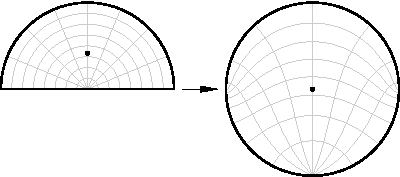
\includegraphics{figures/riemannmap}
\caption{Pemetaan Riemann untuk setengah cakram atas dengan $p=(\sqrt{2}-1)i$.%
\label{fig:riemannmap}}
\end{myfig}

Bukti teorema tersebut merupakan contoh luar biasa tentang menyelesaikan
suatu masalah dengan merumuskan masalah ekstremal terkait.  Fungsi $f$
dalam teorema memaksimumkan
$\sabs{f'(p)}$ di antara pemetaan holomorfik injektif yang membawa $p$ ke $0$.
Kita akan membuktikan bahwa memaksimumkan $\sabs{f'(p)}$ ekuivalen dengan $f$
surjektif:
Untuk setiap pemetaan yang tidak surjektif, kita mencari pemetaan dengan
$\sabs{f'(p)}$ yang lebih besar yang tetap masuk ke dalam cakram.  Pemetaan-pemetaan demikian terbatas,
sehingga teorema Montel memberikan barisan konvergen dengan $\sabs{f'(p)}$
menuju supremum, dan limitnya kemudian harus surjektif.
Mengapa terpikir untuk menggunakan masalah ekstremal ini?  Nah,
memaksimumkan turunan tampak seperti cara yang baik untuk menyebarkan nilai-nilai.
Kita ingin membuat citra sebesar mungkin, dan kita mencapai jarak terjauh jika
kecepatannya terbesar, bukan?

\begin{proof}
Misalkan $\sF$ adalah keluarga fungsi holomorfik injektif (univalen)
$f \colon U \to \D$ sedemikian sehingga $f(p) = 0$.  Kita berusaha mencari
$f \in \sF$ yang surjektif.
Namun, sebelum bergegas menggunakan teorema Montel, kita harus menunjukkan bahwa suatu fungsi
injektif
$f \colon U \to \D$ benar-benar ada,
yakni bahwa $\sF$ takkosong.  Di sinilah kita
menggunakan fakta bahwa $U$ tidak sama dengan bidang kompleks (berdasarkan teorema Liouville, $\sF$
akan kosong jika $U = \C$).  Jika komplemen $U$ memuat himpunan
terbuka, persoalannya akan mudah, tetapi kita hanya dapat menggunakan bahwa komplemen $U$
memuat setidaknya satu titik, dan bahwa $U$ terhubung sederhana.  Kita akan menggunakan
keterhubungan sederhana tersebut untuk mengonstruksi akar kuadrat, karena akar kuadrat merapatkan
berbagai hal.

Misalkan $q \in \C \setminus U$.  Fungsi $z \mapsto z-q$ tidak pernah
nol dan $U$ terhubung sederhana, sehingga $z-q$ memiliki akar kuadrat
holomorfik---terdapat $g \colon U \to \C$ sedemikian sehingga
${\bigl(g(z)\bigr)}^2 = z-q$.
Himpunan $g(U)$ terbuka berdasarkan \hyperref[thm:OMT]{teorema pemetaan terbuka}.
Jika $g(z)=g(\zeta)$, maka ${\bigl(g(z)\bigr)}^2={\bigl(g(\zeta)\bigr)}^2$ sehingga
$z=\zeta$.  Jadi $g$ injektif.  Terlebih lagi,
$g(z)=-g(\zeta)$ juga mengimplikasikan $z=\zeta$.  Jadi, $g(z) =
-g(\zeta)$ tidak pernah terjadi karena $g$ tidak pernah nol.
Dengan kata lain, $g(U) \cap \bigl( - g(U) \bigr) = \emptyset$,
dengan
$- g(U) = \{ w : -w \in g(U) \}$.
Himpunan
$- g(U)$ juga terbuka, sehingga
komplemen $g(U)$ memuat cakram terbuka $\Delta_r(\xi)$.  Dengan demikian,
\begin{equation*}
z \mapsto \frac{r}{g(z)-\xi}
\end{equation*}
memetakan $U$ ke $\D$ dan bersifat injektif.
Dengan mengomposisikannya dengan automorfisme cakram yang tepat,
kita memperoleh pemetaan yang membawa $p$ ke $0$.  Jadi, $\sF$ takkosong.

Baiklah\@.  Sekarang misalkan $f \colon U \to \D$ adalah pemetaan holomorfik injektif
sedemikian sehingga $f(p) = 0$, tetapi $f$ tidak surjektif: Terdapat
$q \in \D \setminus f(U)$.
Ingat bahwa
$\varphi_q(z) = \frac{z-q}{1-\bar{q}z}$ adalah automorfisme dari $\D$ yang
membawa $q$ ke $0$, dan tinjau $\varphi_q \circ f$.  Fungsi ini tidak
nol pada $U$, sehingga
terdapat akar kuadrat holomorfik $g$ pada $U$, yakni,
${\bigl(g(z)\bigr)}^2 = \varphi_q\bigl(f(z)\bigr)$.
Akar kuadrat suatu bilangan di $\D$ tetap berada di $\D$, sehingga $g$
memetakan $U$ ke $\D$.
Jika $g(z)=g(\zeta)$, maka $\varphi_q\bigl(f(z)\bigr)=\varphi_q\bigl(f(\zeta)\bigr)$ dan karena
$\varphi_q \circ f$ injektif, $z=\zeta$.  Jadi $g$ injektif.  
Fungsi $g$ membawa $p$ ke salah satu akar dari $-q$.
Definisikan
\begin{equation*}
h = \varphi_{g(p)} \circ g .
\end{equation*}
Secara khusus, $h(p) = 0$, dan $h \in \sF$.
Invers $\varphi_a$ adalah $\varphi_{-a}$, sehingga
$g = \varphi_{-g(p)} \circ h$.
Selanjutnya, turunkan
$\varphi_q \circ f = g^2$ di $p$, dengan memperhatikan bahwa
$\varphi_a'(0) = 1-\sabs{a}^2$:
\begin{multline*}
\bigl(1-\sabs{q}^2\bigr) f'(p)
= \varphi_q'\bigl(f(p)\bigr) f'(p)
= 2 g(p) g'(p)
\\
= 2 g(p) \varphi_{-g(p)}'\bigl(h(p)\bigr) h'(p)
= 2 g(p) \bigl(1-\sabs{g(p)}^2\bigr) h'(p) .
\end{multline*}
Karena ${\bigl(g(p)\bigr)}^2 = -q$,
\begin{equation*}
\sabs{f'(p)} =
\frac{2 \sabs{g(p)} \bigl(1-\sabs{g(p)}^2\bigr)}{1-\sabs{q}^2} \sabs{h'(p)}
=
\frac{2 \sqrt{\sabs{q}}}{1+\sabs{q}} \sabs{h'(p)} .
\end{equation*}
Jika $\sabs{q} < 1$, maka $\frac{2 \sqrt{\sabs{q}}}{1+\sabs{q}} < 1$
(latihan kalkulus).
Dengan kata lain,
\begin{equation*}
\sabs{f'(p)} < \sabs{h'(p)} .
\end{equation*}

Ambil barisan $\{ f_n \}$ dalam
$\sF$ sedemikian sehingga
\begin{equation*}
\lim_{n \to \infty} \sabs{f_n'(p)} = \sup_{f \in \sF} \sabs{f'(p)} .
\end{equation*}
Karena semua fungsi dalam $\sF$ dibatasi oleh $1$,
teorema Montel menyatakan bahwa terdapat subbarisan yang konvergen seragam pada
himpunan-himpunan bagian kompak ke suatu fungsi holomorfik $f$.  Andaikan $\{ f_n \}$ adalah subbarisan tersebut.
Berdasarkan akibat teorema Hurwitz,
\corref{cor:univalentlimit},
fungsi $f$ bersifat injektif atau konstan.  Fungsi itu tidak dapat konstan,
karena $f_n'(p)$ konvergen ke $f'(p)$, yang
tidak dapat nol sebab  
$0 < \sabs{f_n'(p)} \leq \sabs{f'(p)}$ untuk setiap $n$.
Dengan mengambil limit, kita harus memiliki $f(p) = 0$.
Demikian pula,
$\sabs{f(z)} \leq 1$ untuk semua $z \in U$ dengan mengambil limit,
sehingga $f(U) \subset \overline{\D}$.
Berdasarkan \hyperref[thm:OMT]{teorema pemetaan terbuka}, $f(U) \subset \D$, sehingga $f \in
\sF$.  Jika $f$ tidak surjektif, maka fungsi itu bukanlah fungsi yang mencapai
supremum $\sabs{f'(p)}$; lihat konstruksi $h$ di atas.
Jadi $f(U) = \D$, dan $f$ adalah pemetaan yang diinginkan.
Dengan mengalikannya dengan $e^{i\theta}$, kita dapat membuat $f'(p) > 0$.

Ketunggalannya diserahkan sebagai latihan.
\end{proof}

\begin{exbox}
\begin{exercise}
Selesaikan bukti teorema tersebut:
Untuk himpunan terbuka $U \subset \C$ dan $p \in U$ yang diberikan, buktikan
bahwa suatu fungsi biholomorfik 
$f \colon U \to \D$ sedemikian sehingga $f(p) = 0$ dan $f'(p) > 0$ bersifat tunggal jika ada.
\end{exercise}
\end{exbox}

\begin{remark}
Pemetaan dari teorema tersebut dapat berguna, tetapi teorema itu
sendiri tidak memberi tahu Anda cara mengonstruksinya.
Terdapat buku-buku lengkap
yang ditulis mengenai pokok tersebut dan mengumpulkan teknik untuk mengonstruksi
pemetaan-pemetaan ini bagi berbagai jenis domain.
Sebagai contoh, terdapat rumus eksplisit, yang disebut pemetaan
Schwarz--Christoffel, untuk pemetaan yang diberikan oleh setiap poligon.
Kita tidak akan membahas konstruksi-konstruksi ini di sini.
\end{remark}


\begin{remark}
Pertanyaan menarik lain yang tidak akan kita bahas
adalah regularitas batas dari pemetaan tersebut.  Artinya, apakah pemetaan dapat diperluas ke
tutupan $\widebar{U}$, dan seberapa \myquote{baik} pemetaan itu.  Jika $U$
dibatasi oleh kurva Jordan, diketahui bahwa $f$ dapat diperluas menjadi fungsi kontinu pada
$\widebar{U}$.  Jika $U$ memiliki batas mulus (secara lokal berupa grafik fungsi
mulus), maka $f$ dapat diperluas secara mulus ke $\widebar{U}$.
Jika $U$ memiliki batas analitik-real (secara lokal berupa grafik fungsi
analitik-real), maka $f$ dapat diperluas secara holomorfik sedikit melewati batas.
Sekali lagi, kita merujuk pembaca pada literatur yang lebih lanjut.
\end{remark}

\begin{remark}
Dalam bukti, kita hanya menggunakan bahwa $U$ terhubung sederhana untuk 
memperoleh akar kuadrat dari fungsi-fungsi yang tidak pernah nol.  Jadi hasil yang sebenarnya
kita buktikan adalah bahwa keberadaan akar kuadrat pada $U \neq \C$ mengimplikasikan bahwa $U$
biholomorfik dengan $\D$.  Dengan kata lain, keterhubungan sederhana
$U$ ekuivalen dengan keberadaan akar kuadrat.
\end{remark}

\begin{exbox}
\begin{exercise} \label{exercise:explicitriemann}
Carilah secara eksplisit pemetaan biholomorfik tunggal (pemetaan Riemann)
$f \colon U \to \D$
untuk $U$ dan $p$ berikut, yakni,
%%%%%%%%%%%%%%%%%%%%%%%%%%%%%%%%%%%%%%%%%%%%%%%%%%%%%%%%%%%%%%%%%%%%%%%%%%%%%%
sedemikian sehingga $f(p) = 0$ dan $f'(p) > 0$:
\begin{exparts}
\item
Pita $U = \{ z : -1 < \Im z < 1 \}$, $p=0$.
\item
Kuadran $U = \{ z : \Re z > 0 \text{ dan } \Im z > 0 \}$,
$p=\frac{1+i}{\sqrt{2}}$.
\item
Setengah cakram atas $U = \{ z : \sabs{z} < 1 \text{ dan } \Im z > 0 \}$, $p
= (\sqrt{2}-1)i$.  Petunjuk: Mulailah dengan invers dari pemetaan Cayley, dan
jangan dahulu memikirkan $p$.  Lihat \figureref{fig:riemannmap}.
\end{exparts}
\end{exercise}

\begin{exercise}
Misalkan $V \subset \C$ suatu domain terhubung sederhana, dan $V \neq \C$.
Tunjukkan bahwa setiap $f \colon \C \to V$ yang holomorfik adalah konstan.
\end{exercise}

\begin{exercise}
Misalkan $U \subset \C$ suatu domain terhubung sederhana.
Tunjukkan bahwa untuk setiap dua titik $z,w \in U$, terdapat suatu automorfisme
$\psi \in \Aut(U)$ sedemikian sehingga $\psi(z) = w$.
\end{exercise}

\begin{exercise}
\begin{exparts}
\item
Misalkan $U \subset \C$ suatu domain terhubung sederhana, $U \neq \C$,
$p,q \in U$ adalah titik-titik yang berbeda, dan
$f \colon U \to U$ holomorfik sedemikian sehingga $f(p) = p$ dan $f(q)=q$.
Buktikan bahwa $f$ adalah identitas, yakni, $f(z)=z$ untuk semua $z \in U$.
\item
Temukan suatu contoh penyangkal jika $U=\C$.
\end{exparts}
\end{exercise}

\begin{exercise}
Teorema yang menyerupai pemetaan Riemann untuk domain terhubung ganda (domain dengan
lubang) tidaklah benar
(setidaknya tidak dalam bentuk yang paling jelas):
Tunjukkan bahwa cakram tertusuk $\ann(0;0,1) = \D \setminus \{ 0 \}$
dan anulus $\ann(0;1,2)$ tidak biholomorfik.
\end{exercise}

\begin{exercise}
Misalkan $U \subset \C$ suatu domain. Misalkan satu komponen terhubung dari $\C_\infty
\setminus U$ terdiri atas lebih dari satu titik.
\begin{exparts}
\item
Buktikan bahwa $U$ biholomorfik dengan suatu subhimpunan dari $\D$.
\item
Jika $\C_\infty \setminus U$ mempunyai berhingga banyak komponen terhubung, maka
$U$ biholomorfik dengan $\D \setminus K$ untuk suatu himpunan kompak (yang mungkin kosong)
$K \subset \D$, dengan $K$ mempunyai berhingga banyak komponen.
\end{exparts}
Petunjuk: Bagaimana jika komponen tersebut memuat $\infty$?
\end{exercise}

\begin{exercise}
Misalkan $S \subset \C$ suatu subhimpunan tertutup terhitung.
Buktikan bahwa $U = \C \setminus S$ tidak biholomorfik
dengan subhimpunan mana pun dari $\D$. Petunjuk: Suatu himpunan tertutup terhitung memuat titik-titik terisolasi
karena setiap himpunan sempurna takkosong tidak terhitung
(silakan mengasumsikan fakta ini).
\end{exercise}

\begin{exercise}
Buktikan bahwa
jika $f \colon \C \to \C$ holomorfik entire dan injektif, maka $f$
surjektif.
\end{exercise}
\end{exbox}

\subsection{Terhubung sederhana adalah terhubung sederhana \texorpdfstring{$\star$}{*}}

Akhirnya mari kita buktikan bahwa terhubung sederhana (dalam pengertian homologi,
\defnref{defn:simplyconnected:homology}, yang selama ini kita gunakan),
ekuivalen dengan terhubung sederhana dalam pengertian homotopi.
Bukti korolari ini merupakan contoh indah tentang sesuatu yang akan
cukup sulit tanpa
\hyperref[thm:RMT]{teorema pemetaan Riemann}, dan menjadi hampir
trivial dengan teorema pemetaan tersebut.
Gagasan kuncinya ialah bahwa setiap lintasan secara trivial homotopik dengan lintasan nol di
dalam cakram hanya dengan penskalaan. Lihat juga \exampleref{example:homotopydiscsc}.

\begin{cor} \label{cor:simplyconnhard}
Suatu domain $U \subset \C$ terhubung sederhana dalam pengertian homotopi
jika dan hanya jika
domain itu terhubung sederhana dalam pengertian \defnref{defn:simplyconnected:homology}.
\end{cor}

\begin{proof}
\propref{prop:simplyconneasy} menyatakan bahwa jika $U$
terhubung sederhana dalam pengertian homotopi, maka $U$ terhubung sederhana
dalam pengertian homologi. Jadi mari kita buktikan arah sebaliknya.

Misalkan $U$ terhubung sederhana dalam
pengertian homologi.
Misalkan $\gamma \colon [a,b] \to U$ suatu fungsi kontinu dengan
$\gamma(a)=\gamma(b)$. Kita ingin menunjukkan bahwa $\gamma$ homotopik dengan suatu
konstanta di $U$.
Teorema pemetaan Riemann menyatakan bahwa $U =
\C$ atau terdapat biholomorfisme $f \colon U \to \D$.

Jika $U = \C$, definisikan homotopi $H \colon [a,b] \times [0,1] \to
\C$ sebagai
\begin{equation*}
H(t,s) = (1-s) \gamma(t) .
\end{equation*}
Jika $U \neq \C$, definisikan $H \colon [a,b] \times [0,1] \to U$ sebagai
\begin{equation*}
H(t,s) = f^{-1} \Bigl( (1-s) f \bigl( \gamma(t) \bigr) \Bigr) .
\end{equation*}
Dengan kata lain, kita petakan $U$ ke $\D$ dan mempertimbangkan $f \circ \gamma$.
Kemudian kita definisikan $H$ dengan cara yang sama seperti untuk $\C$, lalu kita
petakan seluruhnya kembali ke $U$.
\end{proof}

\begin{remark}
Sekali lagi perlu kita tekankan bahwa definisi
\myquote{terhubung sederhana dalam pengertian homologi} bukanlah definisi baku.
Definisi itu hanyalah jalan pintas yang kita ambil apabila seseorang ingin
melewati homotopi pada pembacaan pertama. Dalam penggunaan umum (di luar buku ini),
\myquote{terhubung sederhana} selalu
dimaksudkan dalam pengertian homotopi. Lebih lanjut, meskipun untuk domain di $\C$ kedua
konsep itu kebetulan sama, keduanya tidak sama untuk
ruang topologis yang lebih umum.
\end{remark}

\begin{exbox}
\begin{exercise}
Tanpa menggunakan teorema pemetaan Riemann, \corref{cor:simplyconnhard},
atau pemetaan ke cakram dengan cara apa pun, buktikan dengan membangun suatu homotopi eksplisit
bahwa bidang bersayat $\C \setminus (-\infty,0]$ terhubung sederhana dalam
pengertian homotopi; lihat bukti korolari tersebut.
\end{exercise}
\end{exbox}

\subsection{Siklus mengelilingi himpunan kompak dan keterhubungan sederhana}\label{subsec:patharoundK}

Sebagai penerapan kedua dan barangkali jauh kurang jelas dari teorema
pemetaan Riemann,
kita akan membuktikan suatu lema bahwa di sekeliling setiap himpunan kompak dalam suatu domain $U$
kita dapat menemukan suatu siklus yang mengelilingi himpunan kompak ini dan homolog dengan
nol di $U$.
Hal yang menarik adalah bahwa dalam persoalan ini tidak tampak satu pun domain terhubung sederhana,
tetapi kita masih dapat menggunakan
\hyperref[thm:RMT]{teorema pemetaan Riemann}
untuk sangat
menyederhanakan topologi situasinya.
Ada cara-cara yang lebih langsung dan
konstruktif (tetapi tidak kurang teknis) untuk membuktikan lema di bawah ini,\footnote{%
Bukti yang lazim akan menempatkan kisi persegi yang cukup halus pada $\C$, lalu
menunjukkan bahwa jika kita menjumlahkan semua siklus kecil yang perseginya kebetulan beririsan
dengan himpunan kompak tersebut dan menghapus sisi-sisi yang terhitung ganda, kita memperoleh siklus yang diinginkan.}
tetapi saya mempunyai kegemaran yang tidak rasional untuk menggunakan teorema pemetaan, dan bagaimanapun
ini buku saya.

Lema ini akan memungkinkan kita menyelesaikan bukti bahwa domain-domain yang
terhubung sederhana di $\C$ tepat merupakan domain-domain
yang komplemennya di $\C_\infty$ terhubung. Artinya, kita akan membuktikan
arah sebaliknya dari \propref{prop:scbycomplementeasy}. Pertama, lemanya.

\begin{lemma}\label{lemma:patharoundK}
Misalkan $U \subset \C$ terbuka dan misalkan $K \subset U$ kompak dan
takkosong.
Maka terdapat suatu siklus
$\Gamma$ di $U \setminus K$ sedemikian sehingga $n(\Gamma;z) = 1$ untuk semua $z \in K$ dan
$n(\Gamma;z) = 0$ untuk semua $z \in \C \setminus U$ ($\Gamma$ homolog dengan
nol di $U$), dan sedemikian sehingga $n(\Gamma;z)$ bernilai $0$ atau $1$ untuk semua $z \notin
\Gamma$.
\end{lemma}

Gagasan intuitif buktinya cukup sederhana. Misalkan $K$
terhubung.
Bawa satu titiknya ke takhingga melalui suatu LFT
(suatu inversi).
Kemudian gunakan teorema pemetaan Riemann untuk memetakan komplemen $K$ ke
cakram (atau beberapa cakram).
Lalu lintasannya adalah lingkaran berorientasi terbalik (searah jarum jam) yang sangat dekat dengan batas cakram
untuk \myquote{mengelilingi} (setelah inversinya dibalik) apa yang berada
\myquote{di luar cakram,} yakni, lintasan itu akan mengelilingi $K$.
Komplemen dari $U$
bersesuaian dengan suatu himpunan kompak di dalam cakram sehingga dengan cara ini kita tidak akan
\myquote{mengelilingi} komplemen dari $U$.
Kemudian kita mengulangi prosedur tersebut untuk semua komponen $K$. Lihat
\figureref{fig:cyclearoundcompact}. Sebagaimana dapat diduga,
kita menjumpai sejumlah kesulitan teknis seperti kemungkinan $K$ mempunyai
takhingga banyak komponen terhubung, kemungkinan komplemen dari $K$ yang terhubung mempunyai banyak komponen,
dan tentu saja kenyataan bahwa gagasan intuitif yang samar itu menarik,
tetapi kita perlu sungguh-sungguh melakukan perhitungan rinci untuk membuktikan sesuatu.

\begin{myfig}
\subimport*{figures/}{cyclearoundcompact.pdf_t}
\caption{Gagasan bukti: Komplemen dari $K$ beserta takhingga dipetakan ke
bagian dalam cakram oleh teorema pemetaan Riemann. Inversinya adalah
$\varphi$ dan $\psi$ adalah pemetaan dari teorema Riemann.
Bagian luar cakram di sebelah kanan bukan benar-benar citra dari $K$, tetapi
secara intuitif dapat dipandang demikian (karena itu tanda petiknya).\label{fig:cyclearoundcompact}}
\end{myfig}

\begin{proof}
Pertama-tama kita perluas $K$ agar
hanya mempunyai berhingga banyak komponen. Untuk $r > 0$ yang cukup kecil, kita menutupi
$K$ dengan berhingga banyak cakram $\Delta_r(z)$ sedemikian sehingga $\overline{\Delta_r(z)}
\subset U$. Secara khusus, untuk suatu $z_1,\ldots,z_m$,
\begin{equation*}
K' =
\overline{\Delta_r(z_1)}
\cup \cdots \cup
\overline{\Delta_r(z_m)}
\end{equation*}
merupakan subhimpunan kompak dari $U$ dan $K \subset K'$.
Karena $K'$ merupakan gabungan berhingga banyak cakram tertutup, himpunan tersebut mempunyai
berhingga banyak komponen topologis.
Jika kita menemukan suatu $\Gamma$ di $U$ yang mengelilingi $K'$, maka kita selesai karena $K \subset K'$.

Misalkan $K_1,\ldots,K_n$ adalah komponen-komponen dari $K'$.
Komponen-komponen itu tertutup, dan karena jumlahnya berhingga,
$K_2 \cup \cdots \cup K_n$ juga tertutup.
Jika kita membuktikan lema untuk himpunan kompak terhubung $K_1$ dan
himpunan terbuka $U \setminus ( K_2 \cup \cdots \cup K_n )$ guna menemukan suatu siklus
$\Gamma_1$, maka kita menyatakan bahwa kita selesai: Kita dapat mengulangi prosedur tersebut
untuk setiap $K_j$ guna menemukan $\Gamma_j$ dan mengambil $\Gamma = \Gamma_1 + \cdots +
\Gamma_n$. Karena $\Gamma_j$ melilit tepat satu kali setiap titik dari $K_j$
dan tidak melilit titik mana pun dari $K_\ell$ untuk $\ell \neq j$,
maka $\Gamma$ akan melilit tepat satu kali setiap titik dari $K'$,
dan tetap homolog dengan nol di $U$.

Jadi, tanpa mengurangi keumuman, asumsikan bahwa $K$ terhubung.
Asumsikan pula bahwa $0 \in K$. Jika $K= \{0 \}$, kita selesai secara trivial, jadi
asumsikan $K$ terdiri atas lebih dari satu titik.
Misalkan $\varphi \colon \C_\infty \to \C_\infty$ adalah LFT inversi\@:
$\varphi(z) = \nicefrac{1}{z}$ untuk $z \in \C \setminus \{ 0 \}$,
$\varphi(0) = \infty$, dan $\varphi(\infty) = 0$.
Karena merupakan LFT, $\varphi$ adalah pemetaan biholomorfik dari
$\C_\infty$ ke dirinya sendiri, dengan $\varphi^{-1} = \varphi$. Misalkan
\begin{equation*}
V = \varphi(\C_\infty \setminus K) .
\end{equation*}
Perhatikan bahwa $\infty \notin V$, $0 \in V$, $V \neq \C$ ($K$ terdiri atas lebih dari satu
titik), dan
$\C_\infty \setminus V = \varphi(K)$ terhubung.
Jadi setiap komponen terhubung dari $V$ merupakan suatu domain terhubung sederhana
menurut \propref{prop:scbycomplementeasy} (latihan).
Karena kita dapat mengasumsikan bahwa $K$ merupakan gabungan berhingga banyak cakram tertutup,
$\C_\infty \setminus K$ dan karenanya $V$ mempunyai berhingga banyak komponen terhubung.
Misalkan $V_1,\ldots,V_m$ adalah komponen-komponen terhubung
dari $V$.
Menurut teorema pemetaan Riemann, terdapat
suatu pemetaan biholomorfik dari $V_j$ ke $\Delta_1(q_j)$,
dengan $q_1,\ldots,q_m$ beberapa titik yang
cukup berjauhan sehingga cakram-cakram tersebut saling lepas.
Tuliskan $D = \Delta_1(q_1) \cup \cdots \cup \Delta_1(q_m)$.
Dengan kata lain, terdapat
suatu $\psi \colon V \to D$ yang biholomorfik. Kita dapat mengatur agar $q_1=0$
dan $\psi(0)=0$.

Himpunan $\C_\infty \setminus U$ kompak: Himpunan itu merupakan subhimpunan tertutup dari
himpunan kompak $\C_\infty$. Karena $\varphi$ kontinu,
$\varphi(\C_\infty \setminus U)$ kompak dan merupakan subhimpunan dari $V$.
Dan karena $\psi$ kontinu,
\begin{equation*}
S = \psi\bigl(\varphi(\C_\infty \setminus U)\bigr)
\end{equation*}
merupakan subhimpunan kompak dari $D$. Terdapat suatu $r < 1$ sedemikian sehingga
\begin{equation*}
S \subset \Delta_r(q_1) \cup \cdots \cup \Delta_r(q_m) .
\end{equation*}
Pertimbangkan lintasan-lintasan $\gamma_j(t) = q_j + r e^{-it}$ untuk $t \in
[0,2\pi]$,
yakni, $\gamma_j = -\partial
\Delta_r(q_j)$.
Misalkan $\Gamma_j=\varphi^{-1} \circ \psi^{-1} \circ \gamma_j$, dan $\Gamma = \Gamma_1 +
\cdots + \Gamma_m$.

Mari kita hitung bilangan lilitnya.
Untuk setiap $p$ yang tidak terletak pada $\Gamma$, hitung
bilangan lilit (lihat \propref{prop:usubst}):
\begin{multline*}
n(\Gamma;p) =
\sum_{j=1}^m
\frac{1}{2\pi i}
\int_{\varphi^{-1} \circ \psi^{-1} \circ \gamma_j}
\frac{1}{z-p} \, dz
=
\sum_{j=1}^m
\frac{1}{2\pi i}
\int_{\psi^{-1} \circ \gamma_j}
\frac{-1}{(1-\zeta p) \zeta} \, d\zeta
\\
=
\sum_{j=1}^m
\frac{1}{2\pi i}
\int_{\gamma_j}
\frac{-1}{ \bigl( 1-\psi^{-1}(\xi)p \bigr)
\,
\psi^{-1}(\xi)
\,
\psi' \bigl(\psi^{-1}(\xi)\bigr)} \, d \xi .
\end{multline*}

Pertama misalkan $p \in \C \setminus U$.
Fungsi
\begin{equation*}
h(\xi) =
\frac{-1}{ \bigl( 1-\psi^{-1}(\xi)p \bigr)
\,
\psi^{-1}(\xi)
\,
\psi' \bigl(\psi^{-1}(\xi)\bigr)}
\end{equation*}
yang didefinisikan pada $D$ mempunyai dua kutub: satu di $\psi(\nicefrac{1}{p})$ dan satu
di $q_1=0$ (faktor ketiga di penyebut tidak pernah nol).
Keduanya merupakan kutub sederhana sebagaimana mudah diperiksa, dan residunya adalah (dengan menggunakan
\propref{prop:residuesimpleratio})
\begin{equation*}
\operatorname{Res}(h;0) =
\frac{-1}{ \bigl( 1-\psi^{-1}(0)p \bigr)
\,
\psi' \bigl(\psi^{-1}(0)\bigr)}
\,
\frac{1}{\frac{1}{\psi'(\psi^{-1}(0))}}
=
-1
\end{equation*}
dan
\begin{equation*}
\operatorname{Res}\bigl(h;\psi(\nicefrac{1}{p})\bigr)
=
\frac{-1}{
\psi^{-1}\bigl(\psi(\nicefrac{1}{p})\bigr)
\,
\psi' \bigl(\psi^{-1}(\psi(\nicefrac{1}{p}))\bigr)
}
\,
\frac{1}{
\frac{-1}{\psi'(\psi^{-1}(\psi(1/p)))}
\, p
}
=
1 .
\end{equation*}
Lintasan $\gamma_1$ mengelilingi $q_1=0$.
Suatu $\gamma_j$ mengelilingi
$\psi(\nicefrac{1}{p})$, karena $r$ dipilih cukup besar
tepat agar lingkaran-lingkaran $\gamma_j$ mengelilingi $S$, yakni titik-titik yang
merupakan citra dari $\C \setminus U$,
khususnya, $\psi(\nicefrac{1}{p})=\psi\bigl(\varphi(p)\bigr)$.
Jumlah residunya nol, jadi
menurut \hyperref[thm:residue]{teorema residu},
\begin{equation*}
n(\Gamma;p) = 0 .
\end{equation*}

Selanjutnya misalkan $p \in K$. Seperti sebelumnya,
$n(\Gamma;p) =
\sum_j
\frac{1}{2\pi i}
\int_{\gamma_j} h(\xi) \, d\xi$.
Karena $p \in K$, $\psi^{-1}(\xi) \neq \nicefrac{1}{p}$ untuk semua $\xi \in D$,
sehingga $h$ hanya mempunyai kutub di $0$.
Karena $\gamma_1$ menelusuri lingkaran itu dengan orientasi terbalik,
\begin{equation*}
n(\Gamma;p) =
\sum_{j=1}^m
\frac{1}{2\pi i}
\int_{\gamma_j} h(\xi) \, d\xi
=
\frac{1}{2\pi i}
\int_{\gamma_1} h(\xi) \, d\xi
= - \operatorname{Res}(h;0) = 1 .
\end{equation*}

Jika $p$ adalah titik lain mana pun yang tidak terletak pada $\Gamma$, maka $n(\Gamma;p)$
bernilai $0$ atau $1$, bergantung pada apakah terdapat kutub di
$\psi(\nicefrac{1}{p})$ dan apakah $\Gamma$ mengelilinginya atau tidak.
\end{proof}

\begin{exbox}
\begin{exercise}
Buktikan bahwa jika $K \subset \C_\infty$ kompak dan terhubung, maka
setiap komponen dari $\C_\infty \setminus K$ merupakan domain terhubung sederhana.
Petunjuk: Buktikan bahwa komplemen dari setiap komponen ini terhubung.
\end{exercise}
\end{exbox}

Sekarang kita dapat membuktikan karakterisasi topologis yang paling sederhana bagi
domain-domain terhubung sederhana di $\C$.

\begin{thm} \label{cor:scbycomplementhard}
Misalkan $U \subset \C$ suatu domain. Maka
$\C_\infty \setminus U$ terhubung jika dan hanya jika $U$ terhubung sederhana.
\end{thm}

\begin{proof}
Arah maju adalah \propref{prop:scbycomplementeasy}. Mari kita kerjakan
arah mundur melalui kontraposisi. Misalkan $\C_\infty
\setminus U$ tidak terhubung. Maka terdapat dua himpunan tertutup takkosong yang saling lepas
$S$ dan $K$ sedemikian sehingga $S \cup K = \C_\infty \setminus U$.
Asumsikan $\infty \in S$.
Himpunan $U' = U \cup K$ terbuka karena $S$ tertutup, $U' \subset \C$,
dan $K \subset U'$ kompak. Terapkan lema untuk menemukan suatu siklus
$\Gamma$ di $U = U' \setminus K$ sedemikian sehingga $n(\Gamma;z) = 1$ untuk semua $z \in
K$. Dengan kata lain, $\Gamma$ tidak homolog dengan nol di $U$.
\end{proof}

\begin{exbox}
\begin{exercise}
Misalkan $K \subset \C$ kompak dan terhubung, $\C \setminus K$
terhubung, dan $K$ terdiri atas lebih dari satu titik.
Buktikan bahwa terdapat suatu pemetaan biholomorfik
$\psi \colon \C \setminus K \to \C \setminus \overline{\D}$.
\end{exercise}

\begin{exercise}
Bangun suatu contoh himpunan kompak $K \subset \C$ dengan suatu komponen terhubung $K_1$
yang mempunyai sifat berikut.
Untuk setiap siklus $\Gamma$ di $\C \setminus K$ sedemikian sehingga $n(\Gamma;z)=1$ untuk
semua $z \in K_1$,
terdapat suatu $\zeta \in K \setminus K_1$ dengan $n(\Gamma;\zeta)=1$.
Mengapa contoh ini tidak bertentangan dengan konstruksi dalam bukti lema tersebut?
\end{exercise}

\begin{exercise}
Misalkan $\{ f_n \}$ suatu barisan fungsi holomorfik pada himpunan terbuka
$U \subset \C$ yang konvergen seragam pada subhimpunan kompak menuju suatu fungsi takkonstan
$f \colon U \to \C$. Misalkan $K \subset U$ suatu himpunan kompak. Buktikan bahwa
untuk setiap lingkungan terbuka $V$ dari $K$ di $U$ (jadi $K \subset V \subset U$), terdapat
lingkungan terbuka yang lebih kecil $W$ (jadi $K \subset W \subset V$) dan suatu $N \in \N$
sedemikian sehingga $f$ dan $f_n$ mempunyai jumlah nol yang sama di $W$ untuk semua
$n \geq N$.
\end{exercise}

\begin{exercise}
Diberikan himpunan terbuka $U \subset \C$, himpunan kompak takkosong $K \subset U$, dan $\delta > 0$,
buktikan bahwa
terdapat suatu siklus $\Gamma$ di $U \setminus K$ yang homolog dengan nol di $U$,
sedemikian sehingga $n(\Gamma;z)$ bernilai $0$ atau $1$ untuk semua $z \notin \Gamma$,
sedemikian sehingga
$n(\Gamma;z) = 1$ untuk semua $z \in K$,
dan sedemikian sehingga untuk setiap $p \in \Gamma$ terdapat suatu $q \in K$ sehingga
$\sabs{p-q} < \delta$ ($\Gamma$ berada dalam jarak $\delta$ dari $K$).
\end{exercise}

\begin{exercise}\label{exercise:rootgivesscII}
Misalkan $U \subset \C$ suatu domain.
\begin{exparts}
\item
Buktikan bahwa jika $U$ tidak terhubung sederhana, maka terdapat suatu $p \in \C
\setminus U$ dan suatu siklus $\Gamma$ di $U$ sedemikian sehingga $n(\Gamma;p)=1$.
\item
Tetapkan suatu bilangan bulat $k \geq 2$.
Misalkan untuk setiap $f \colon U \to \C$ yang holomorfik dan tidak pernah nol,
terdapat suatu $g \colon U \to \C$ yang holomorfik sedemikian sehingga $g^k = f$.
Buktikan bahwa $U$ terhubung sederhana.
Petunjuk: Lihat \exerciseref{exercise:rootgivesscI} untuk suatu petunjuk.
\end{exparts}
\end{exercise}
\end{exbox}

%%%%%%%%%%%%%%%%%%%%%%%%%%%%%%%%%%%%%%%%%%%%%%%%%%%%%%%%%%%%%%%%%%%%%%%%%%%%%%
%%%%%%%%%%%%%%%%%%%%%%%%%%%%%%%%%%%%%%%%%%%%%%%%%%%%%%%%%%%%%%%%%%%%%%%%%%%%%%
%%%%%%%%%%%%%%%%%%%%%%%%%%%%%%%%%%%%%%%%%%%%%%%%%%%%%%%%%%%%%%%%%%%%%%%%%%%%%%

\chapter{Fungsi Harmonik} \label{ch:harmonic}

\begin{myepigraph}
Jika Anda tidak dapat menyingkirkan kerangka keluarga, sekalian saja buatlah ia
menari.

---George Bernard Shaw
\end{myepigraph}

%%%%%%%%%%%%%%%%%%%%%%%%%%%%%%%%%%%%%%%%%%%%%%%%%%%%%%%%%%%%%%%%%%%%%%%%%%%%%%

\section{Fungsi harmonik}
\label{sec:harmonic}

Sejauh ini, kita mengkaji fungsi holomorfik sebagai fungsi bernilai kompleks.
Namun, untuk melakukan analisis diperlukan pertidaksamaan, sedangkan bilangan kompleks tidak
terurut. Mari kita tinjau bagian real dan imajiner dari fungsi holomorfik,
yang disebut fungsi harmonik. Menariknya, fungsi
harmonik sering muncul dalam matematika terapan, misalnya sebagai distribusi panas
keadaan tunak atau distribusi potensial elektrostatik di daerah tanpa
muatan. Fungsi harmonik digunakan untuk mempelajari
fungsi holomorfik dan sebaliknya, fungsi holomorfik digunakan untuk
mempelajari fungsi harmonik.

Sebagian besar hasil
yang akan kita buktikan untuk fungsi harmonik merupakan analog dari hasil
untuk fungsi holomorfik. Pembaca dianjurkan
mencari hubungan-hubungan ini.
Sebagaimana hewan paling baik dipelajari di habitat alaminya,
banyak hasil yang kita buktikan untuk fungsi holomorfik
lebih baik dipahami sebagai hasil tentang fungsi harmonik.
Meskipun demikian, hasil-hasil untuk fungsi harmonik tidak
selalu merupakan penerapan sederhana dari apa yang sudah dibuktikan untuk fungsi
holomorfik, dan bahkan
pernyataan atau bukti hasil-hasil analognya dapat cukup berbeda.
Fungsi harmonik sedikit lebih umum daripada bagian real dan
imajiner fungsi holomorfik. Fungsi tersebut merupakan bagian real dan imajiner
dari fungsi holomorfik hanya secara lokal, tetapi mungkin tidak secara global.


\subsection{Bagian real dan imajiner dari fungsi holomorfik}

\begin{defn}
Misalkan $U \subset \C$ terbuka.
Suatu pemetaan $C^2$ (disingkat demikian karena terdiferensialkan (secara real) dua kali secara kontinu), $f \colon U \to \R$,
disebut \emph{\myindex{harmonik}} jika
\glsadd{not:laplacian}%
\begin{equation*}
\nabla^2 f =
\frac{\partial^2 f}{\partial x^2} +
\frac{\partial^2 f}{\partial y^2} = 0
\quad \text{ pada $U$.}
\end{equation*}
\end{defn}

Operator $\nabla^2$, yang kadang ditulis $\Delta$,
adalah \emph{\myindex{Laplacian}}.\footnote{%
Laplacian didefinisikan di $\R^n$ untuk setiap $n$ melalui
$\nabla^2 f =
\frac{\partial^2 f}{\partial x_1^2} + \cdots +
\frac{\partial^2 f}{\partial x_n^2}$, sehingga
terdapat fungsi harmonik di setiap dimensi.
Kita tertarik pada bidang kompleks, $n=2$,
yang ternyata sangat berbeda dari kasus $n \geq 3$.
Ketika $n \geq 3$, teorinya jauh lebih sedikit berkaitan dengan analisis kompleks.}
Operator ini adalah teras matriks Hessian. Berguna untuk
mencatat bahwa
\begin{equation*}
4
\frac{\partial^2}{\partial \bar{z}\partial z} f =
4
\left[
\frac{1}{2}
\left(
\frac{\partial}{\partial x} + i
\frac{\partial}{\partial y}
\right)
\right]
\left[
\frac{1}{2}
\left(
\frac{\partial}{\partial x} - i
\frac{\partial}{\partial y}
\right)
\right]
f
=
\left[
\frac{\partial^2}{\partial x^2} +
\frac{\partial^2}{\partial y^2}
\right]
f
=
\nabla^2 f .
\end{equation*}

Dengan kata lain, $f$ harmonik jika dan hanya jika
$\frac{\partial f}{\partial z}$ holomorfik.
Jadi misalkan $f$ harmonik.
Secara lokal (di suatu lingkungan), kita menemukan suatu
primitif $g$ dari $\frac{\partial f}{\partial z}$, dan kita tuliskan
\begin{equation*}
f(z) = g(z) + c(z) ,
\end{equation*}
dengan $g$ holomorfik, $c$ setidaknya $C^2$, dan $\frac{\partial c}{\partial z} \equiv 0$.
Misalkan $h = \bar{c}$ adalah konjugat kompleks dari $c$. Maka
\begin{equation*}
\frac{\partial h}{\partial \bar{z}}
=
\frac{\partial \bar{c}}{\partial \bar{z}}
=
\overline{
\frac{\partial c}{\partial z}
}
=
0 ,
\end{equation*}
sehingga $h$ holomorfik. Jadi, secara lokal, kita telah menemukan $g$ dan $h$ yang holomorfik
sedemikian sehingga
\begin{equation*}
f(z) = g(z) + \overline{h(z)} .
\end{equation*}
Pertimbangkan fungsi holomorfik $\varphi(z) = g(z) + h(z)$.
Karena $f$ bernilai real,
\begin{equation*}
f(z) = \Re f(z) =
\frac{g(z) + \overline{h(z)} + \overline{g(z)}+h(z)}{2}
=
\frac{g(z) + h(z) + \overline{g(z)+h(z)}}{2}
=
\Re \varphi(z) .
\end{equation*}
Jadi setiap fungsi harmonik $f$ secara lokal merupakan bagian real dari suatu fungsi
holomorfik. Demikian pula, $f$ secara lokal merupakan bagian imajiner dari suatu fungsi
holomorfik.
Semua ini hanya berlaku di suatu lingkungan. Kita belum tentu dapat menemukan satu
$\varphi$ (yakni $g$ dan $h$ di atas) pada seluruh
domain $U$, kecuali $U$ terhubung sederhana. Jika tidak, kita selalu dapat
memilih suatu lingkungan terhubung sederhana, misalnya sebuah cakram.
Jika $U$ terhubung sederhana, maka
$\frac{\partial f}{\partial z}$ mempunyai suatu primitif di $U$,
dan perhitungan di atas menghasilkan
proposisi berikut.

\begin{prop} \label{prop:harmconj}
Misalkan $U \subset \C$ suatu domain terhubung sederhana dan $f \colon U \to \R$ suatu
fungsi harmonik. Maka terdapat suatu $\varphi \colon
U \to \C$ yang holomorfik sedemikian sehingga $f = \Re \varphi$.
\end{prop}

Sebaliknya,
misalkan $f$ adalah bagian real dari suatu fungsi holomorfik $\varphi$:
\begin{equation*}
f(z) = \Re \varphi(z) =
\frac{1}{2}\bigl( \varphi(z) + \overline{\varphi(z)} \bigr) .
\end{equation*}
Perhatikan bahwa
\begin{equation*}
\nabla^2 =
4 \frac{\partial^2}{\partial \bar{z} \partial z}
=
4 \frac{\partial^2}{\partial z \partial \bar{z}} .
\end{equation*}
Maka
\begin{equation*}
\nabla^2 f =
4 \frac{\partial^2}{\partial \bar{z} \partial z}
\left(
\frac{1}{2}\bigl( \varphi(z) + \overline{\varphi(z)} \bigr)
\right)
=
2
\left(
\frac{\partial}{\partial z}
\left(
\frac{\partial}{\partial \bar{z}}
\varphi(z)
\right)+
\frac{\partial}{\partial \bar{z}}
\left(
\frac{\partial}{\partial z}
\overline{\varphi(z)}
\right)
\right)
=
0 .
\end{equation*}
Dengan demikian kita telah membuktikan karakterisasi fungsi
harmonik berikut.

\begin{prop} \label{prop:harmanal}
Misalkan $U \subset \C$ terbuka dan $f \colon U \to \R$ suatu fungsi.
\begin{enumerate}[(i)]
\item
Fungsi $f$ harmonik jika dan hanya jika
untuk setiap titik $p \in U$, terdapat suatu lingkungan terbuka $V$ dari $p$ dan suatu
$\varphi \colon V \to \C$ yang holomorfik sedemikian sehingga $f = \Re \varphi$
pada $V$.
\item
Fungsi $f$ harmonik jika dan hanya jika
untuk setiap $p \in U$, terdapat suatu ekspansi deret pangkat
\begin{equation*}
f(z) =
c_0
+
\sum_{n=1}^\infty c_n {(z-p)}^n + \bar{c}_n {(\overline{z-p})}^n
\end{equation*}
yang konvergen mutlak secara seragam
pada setiap cakram tertutup $\overline{\Delta_r(p)} \subset U$.
\end{enumerate}
\end{prop}

Karena fungsi holomorfik
terdiferensialkan takhingga kali, demikian pula fungsi harmonik.
Sesungguhnya, di atas kita melihat bahwa fungsi harmonik mempunyai suatu deret pangkat real
(deret pangkat dalam $x$ dan $y$, atau secara ekuivalen dalam $z$ dan $\bar{z}$)
dan karena itu bersifat analitik real.

\begin{prop}
Jika $U \subset \C$ terbuka dan $f \colon U \to \R$ harmonik, maka $f$ terdiferensialkan (secara real) takhingga kali.
\end{prop}

Dimulai dengan suatu fungsi harmonik $f$, menemukan suatu fungsi holomorfik yang
bagian realnya adalah $f$ berarti menemukan fungsi harmonik lain $g$ sedemikian sehingga $f+ig$
holomorfik.

\begin{defn}
Misalkan $U \subset \C$ terbuka dan $f \colon U \to \R$ harmonik.
Jika $g \colon U \to \R$ harmonik dan $f + i g$ holomorfik,
maka $g$ disebut \emph{\myindex{konjugat harmonik}} dari $f$.
\end{defn}

\propref{prop:harmconj}
menyatakan bahwa setiap fungsi harmonik pada suatu domain terhubung sederhana
mempunyai suatu konjugat harmonik. Di sisi lain, pada bidang tertusuk
$\C \setminus \{ 0 \}$, fungsi harmonik $\log \sabs{z}$
tidak mempunyai konjugat harmonik. Seandainya fungsi itu mempunyai konjugat harmonik,
maka $\log$ akan mempunyai suatu cabang di $\C \setminus \{0\}$, padahal tidak.
Lihat \figureref{fig:loggraph}, dengan grafik bagian real di sebelah kiri
kontinu, tetapi bagian imajiner yang bersesuaian bukanlah suatu fungsi.
Bahwa kita tidak dapat menemukan konjugat lain untuk $\log \sabs{z}$
mengikuti proposisi berikut.

\begin{prop} \label{prop:harmonicconjdifferbyconst}
Misalkan
$U \subset \C$ suatu domain dan $f \colon U \to \R$ harmonik.
Jika $g_1$ dan $g_2$ adalah dua konjugat harmonik dari $f$,
maka $g_1 = g_2 + C$ untuk suatu $C \in \R$.
\end{prop}

Buktinya trivial: Hipotesisnya menyiratkan bahwa
\begin{equation*}
\frac{(f + i g_1) - (f + i g_2)}{i} =  g_1-g_2
\end{equation*}
holomorfik dan bernilai real pada $U$, sehingga konstan.

Bagian real dan imajiner dari suatu fungsi holomorfik bersifat harmonik;
namun, modulus $\sabs{f(z)}$ tidak. Tidak perlu khawatir,
$\log \sabs{f(z)}$ harmonik, setidaknya di tempat $f$ tidak nol.
Fakta bahwa $\log \sabs{f(z)}$ harmonik sama bergunanya
dengan fakta bahwa bagian real dan imajiner dari $f$ harmonik.
Buktinya diserahkan sebagai latihan.

\begin{prop} \label{prop:logharm}
Misalkan $U \subset \C$ terbuka, $f \colon U \to \C$ holomorfik
dan tidak pernah nol. Maka
\begin{equation*}
z \mapsto \log \sabs{f(z)}
\end{equation*}
harmonik.
\end{prop}

\begin{savenotes}
\begin{exbox}
\begin{exercise}
Buktikan \propref{prop:logharm}.
\end{exercise}

\begin{exercise}
Tunjukkan bahwa fungsi-fungsi $x$ dan $y$ berikut (dengan
$z = x+iy$) bersifat
harmonik (baik pada $\C$ maupun pada himpunan yang diberikan)
dan temukan konjugat harmoniknya.
\smallskip
\begin{expartshor}{5}
\item
$y$
\item
$xy$
\item
$\arctan(y/x)$ pada $x \neq 0$
\item
$\frac{x}{x^2+y^2}$ pada $z \neq 0$
\end{expartshor}
\end{exercise}

\begin{exercise}
Misalkan $U \subset \C$ suatu domain terhubung sederhana
dan $f \colon U \to \R$ suatu fungsi harmonik. Buktikan bahwa terdapat
suatu fungsi holomorfik $\varphi \colon U \to \C$ sedemikian sehingga
$f(z) = \log \sabs{\varphi(z)}$.
\end{exercise}

\begin{exercise}
Misalkan $U,V \subset \C$ himpunan-himpunan terbuka dan
$f \colon U \to V$ holomorfik. Buktikan:
\begin{exparts}
\item
Jika $g \colon V \to \R$ harmonik, maka
$g \circ f$ harmonik.
\item
Misalkan $f$ suatu biholomorfisme antara $U$ dan $V$.
Maka $g \colon V \to \R$ harmonik jika dan hanya jika
$g \circ f$ harmonik.
\end{exparts}
\end{exercise}

\begin{exercise}
Buktikan bahwa jika $f \colon \D \to \R$ harmonik, maka
$f(\nicefrac{z}{\sabs{z}^2})$ harmonik di $\C \setminus
\overline{\D}$.
\end{exercise}

\begin{exercise}
Misalkan $U \subset \C$ suatu domain dan
$f \colon U \to \C$ holomorfik. Buktikan bahwa
jika $z \mapsto \sabs{f(z)}^2$ harmonik, maka $f$ konstan.
\end{exercise}

\begin{exercise}
Misalkan $f \colon \C \to \R$ harmonik.
\begin{exparts}
\item
Tunjukkan bahwa terdapat
suatu $F \colon \C \setminus \{ 0 \} \to \C$ yang holomorfik
sedemikian sehingga $F=f$ pada $\partial \D$.
\item
Tunjukkan bahwa jika $F$ dari bagian a) mempunyai kutub di titik asal, maka $f$
adalah bagian real dari suatu polinomial holomorfik.
\end{exparts}
\end{exercise}

\begin{exercise}
Misalkan $U \subset \C$ terbuka, $\overline{\D} \subset U$,
dan $f \colon U \to \R$ harmonik. Ekspansikan
$f$ sebagai deret pangkat real di titik asal seperti dalam \propref{prop:harmanal}, dan temukan rumus
untuk $c_n$ dalam suku-suku
suatu integral mengelilingi $\partial \D$.
\end{exercise}

% Sebaiknya ini menjadi latihan terakhir dalam exbox ini,
% agar catatan kaki (karena savenotes) muncul
% (kemungkinan besar) pada halaman kanan.
\begin{exercise}\label{exercise:Liouvilleharmonic}
\pagebreak[2]
Buktikan teorema Liouville\footnote{%
Lihat
Nelson, Edward
\emph{A proof of Liouville's theorem.}
Proc.\ Amer.\ Math.\ Soc.\ {\textbf{12}} (1961), 995
(salah satu makalah terbitan terpendek) untuk
suatu bukti elegan bagi fungsi terbatas.
Namun Anda tidak dapat menggunakannya karena Anda belum mempunyai
alat yang diperlukan.}\index{teorema Liouville!fungsi harmonik} untuk
fungsi harmonik: Jika $f \colon \C \to \R$ harmonik
dan taknegatif, maka $f$ konstan.
\end{exercise}
\end{exbox}
\end{savenotes}

\begin{remark}
Seperti dalam \exerciseref{exercise:Liouvilleharmonic},
analog dari \myquote{terbatas} untuk fungsi holomorfik adalah
\myquote{taknegatif}
untuk fungsi harmonik. Bagaimanapun, jika $f$ adalah
fungsi holomorfik terbatas, maka $\log \sabs{f(z)+M}$ atau $\Re f(z) + M$
taknegatif untuk $M$ yang cukup besar. Sebaliknya, jika $\log \sabs{f(z)} \geq
0$, maka $\frac{1}{f(z)}$ terbatas, dan jika $\Re f(z) \geq 0$, maka
$\frac{f(z)-1}{f(z)+1}$ terbatas (dengan mengomposisikan $f$ dengan suatu LFT yang memetakan
setengah bidang kanan ke cakram).
\end{remark}


\begin{remark}
Prosedur di atas, yakni menulis
\begin{equation*}
\frac{\partial^2}{\partial x^2}+ \frac{\partial^2}{\partial y^2} =
4 \frac{\partial^2}{\partial \bar{z} \partial z} ,
\end{equation*}
yaitu suatu jumlah turunan sebagai komposisi dari
turunan-turunan yang berbeda,
sehingga kita dapat mengintegralkan terhadap kedua variabel baru ini, mungkin
terdengar tidak asing. Dalam kasus ini, kita mendapati bahwa suatu $f$ yang harmonik adalah jumlah dari suatu fungsi
dalam $z$ (suatu fungsi holomorfik) dan suatu fungsi dalam $\bar{z}$ (suatu
fungsi antiholomorfik).

Prosedur tersebut serupa dengan solusi D'Alembert bagi persamaan gelombang satu dimensi,
yang mungkin pernah Anda jumpai dalam mata kuliah persamaan diferensial tingkat sarjana.
Operator gelombangnya adalah
$\frac{\partial^2}{\partial t^2}- \frac{\partial^2}{\partial x^2}$ dengan suatu
tanda minus, dengan kita menggunakan $x$ dan $t$ sebagai variabel sesuai tradisi.
Operator gelombang itu terurai sebagai
\begin{equation*}
\frac{\partial^2}{\partial t^2}- \frac{\partial^2}{\partial x^2}
=
\left[ \frac{\partial}{\partial t}- \frac{\partial}{\partial x}
\right]
\left[ \frac{\partial}{\partial t}+ \frac{\partial}{\partial x}
\right] .
\end{equation*}
Jika kita menulis $\mu = x+t$ dan $\eta = x-t$
(yang disebut koordinat karakteristik), maka
\begin{equation*}
\frac{\partial^2}{\partial t^2}- \frac{\partial^2}{\partial x^2}
=
-4 \frac{\partial^2}{\partial \eta \partial \mu} .
\end{equation*}
Seperti sebelumnya, suatu solusi $f$ bagi persamaan gelombang merupakan fungsi
dalam $\mu$ ditambah fungsi dalam $\eta$. Artinya, $f(x,t) = A(\mu) + B(\eta) =
A(x+t)+B(x-t)$, dua gelombang yang merambat dalam arah berlawanan. Fungsi-fungsi
$A$ dan $B$ sama sekali tidak perlu bagus; cukup berupa fungsi yang terdiferensialkan real
dua kali.
Menarik sekali bahwa satu tanda minus yang remeh menimbulkan perbedaan sebesar itu.
\end{remark}

\subsection{Identitas dan prinsip maksimum}

Salah satu konsekuensi dari proposisi-proposisi di atas ialah teorema identitas
untuk fungsi harmonik.
Himpunan nol suatu fungsi harmonik boleh mempunyai titik limit.
Sebagai contoh, $\Re z$ bernilai nol pada seluruh sumbu
imajiner. Namun, himpunan terbuka tetap tidak diperbolehkan bagi fungsi harmonik
takkonstan. Ini sebenarnya merupakan sifat fungsi analitik real, yakni
fungsi yang mempunyai representasi deret pangkat dalam $x$ dan $y$
atau $z$ dan $\bar{z}$, tetapi kita tidak ingin masuk terlalu jauh ke dalam deret pangkat dua
variabel.

\begin{thm}[Identitas]\index{teorema identitas!fungsi harmonik}
Misalkan $U \subset \C$ suatu domain dan $f \colon U \to \R$ suatu fungsi harmonik.
Misalkan $V \subset U$ suatu subhimpunan terbuka takkosong dan $f = 0$ pada $V$. Maka $f
\equiv 0$.
\end{thm}

\begin{proof}
Misalkan $Z_f$ adalah himpunan nol dari $f$ dan misalkan $Z$ adalah penutupan dari interior
$Z_f$ dalam topologi subruang dari $U$.
Himpunan $Z$ takkosong menurut hipotesis, jadi
pertimbangkan suatu $p \in Z$. Pertimbangkan $\Delta_r(p) \subset U$.
Terdapat suatu $h \colon \Delta_r(p) \to \C$ yang holomorfik
sedemikian sehingga $f = \Re h$ pada $\Delta_r(p)$.
Pada suatu subhimpunan terbuka dari cakram tersebut, $f$ bernilai nol.
Jadi fungsi holomorfik $h$ bernilai imajiner murni pada
suatu subhimpunan terbuka dari $\Delta_r(p)$, dan karena itu konstan pada subhimpunan terbuka tersebut.
Menurut \hyperref[thm:identity]{teorema identitas untuk fungsi holomorfik},
$h$, dan karenanya $f$, konstan
pada $\Delta_r(p)$.
Karena $f$ bernilai nol di suatu tempat pada
cakram tersebut dan konstan, fungsi itu bernilai nol pada seluruh cakram.
Jadi $Z$ terbuka.
Karena $Z$ juga tertutup dan $U$ terhubung, $Z=U$.
\end{proof}

Prinsip maksimum sesungguhnya merupakan teorema tentang fungsi harmonik alih-alih
fungsi holomorfik. Kita akan membuktikannya dengan menggunakan fungsi holomorfik
dan teorema pemetaan terbuka (\thmref{thm:OMT})\footnote{%
Bagaimanapun, teorema pemetaan terbuka adalah
versi yang lebih kuat dari prinsip modulus maksimum.},
meskipun terdapat suatu bukti yang lebih alami menggunakan sifat nilai rata-rata,
yang akan kita lihat nanti.

\begin{thm}[Prinsip maksimum]
\index{prinsip maksimum!fungsi harmonik}%
Misalkan $U \subset \C$ suatu domain dan $f \colon U \to \R$
harmonik. Jika $f$ mencapai maksimum lokal (atau minimum lokal) di $U$, maka $f$ konstan.
\end{thm}

\begin{proof}
Misalkan $f$ mencapai maksimum lokal di $p \in U$.
Pernyataan untuk minimum diperoleh dengan mempertimbangkan $-f$.
Misalkan $\Delta_r(p) \subset U$
suatu cakram sedemikian sehingga
pada $\Delta_r(p)$,
$f$ mencapai maksimumnya di $p$.
Terdapat suatu $h \colon \Delta_r(p) \to \C$ yang holomorfik
sedemikian sehingga $f = \Re h$.
Maka $h$ memetakan
$\Delta_r(p)$ ke suatu subhimpunan dari $X = \bigl\{ w \in \C : \Re w \leq f(p) \bigr\}$.
Titik $h(p)$ berada pada batas $X$, karena $\Re h(p)= f(p)$. Oleh sebab itu,
$h\bigl(\Delta_r(p)\bigr)$ tidak terbuka, yang menurut teorema pemetaan terbuka hanya mungkin jika $h$
konstan. Karena $f$ konstan pada $\Delta_r(p)$, fungsi itu konstan pada $U$ menurut
teorema identitas.
\end{proof}

\begin{exbox}
\begin{exercise}
Buktikan bahwa
prinsip maksimum untuk fungsi harmonik menyiratkan prinsip
modulus maksimum untuk fungsi holomorfik.
Petunjuk: Pertimbangkan $\log \sabs{f(z)}$.
\end{exercise}

\begin{exercise}%[\neededexmark]
\label{exercise:maxprincsecondharmonic}
Buktikan versi kedua dari prinsip maksimum: Jika $U \subset \C$
adalah suatu domain terbatas dan
$f \colon \widebar{U} \to \R$ suatu fungsi kontinu
yang harmonik pada $U$,
maka $f$ mencapai maksimum dan minimumnya
pada batas $\partial U$.
\end{exercise}

\begin{exercise}
Misalkan $U \subset \C$ terbuka sedemikian sehingga $\R \cap U \neq \emptyset$
dan $\R \cap U$ terhubung.
Misalkan $f \colon U \to \R$ harmonik
dan himpunan nol dari restriksi $f|_{\R \cap U}$ mempunyai suatu titik limit di
$\R \cap U$. Buktikan bahwa $f|_{\R \cap U} \equiv 0$.
\end{exercise}

\begin{exercise}
Misalkan $U \subset \C$ suatu domain dan
$f \colon U \to \R$ harmonik.
Buktikan bahwa $f(U)$ merupakan suatu interval terbuka atau suatu titik tunggal.
\end{exercise}
\end{exbox}

%%%%%%%%%%%%%%%%%%%%%%%%%%%%%%%%%%%%%%%%%%%%%%%%%%%%%%%%%%%%%%%%%%%%%%%%%%%%%%

\section{Masalah Dirichlet dalam cakram dan penerapannya}

\subsection{Masalah Dirichlet dalam cakram dan kernel Poisson}

Berguna untuk menemukan suatu fungsi harmonik berdasarkan nilai-nilai batas:
Diberikan suatu himpunan terbuka $U \subset \C$
dan suatu $f \colon \partial U \to \R$ yang kontinu,
temukan suatu $g \colon \widebar{U} \to \R$ yang kontinu,
harmonik pada $U$, sedemikian sehingga $g|_{\partial U} = f$.
Persoalan ini disebut \emph{\myindex{masalah Dirichlet}}, dan dapat
diselesaikan untuk banyak (meskipun tidak semua) himpunan terbuka. Jika solusi ada pada suatu
domain terbatas, maka solusi tersebut unik. Pada domain takterbatas, solusi belum tentu
unik; lihat \exerciseref{exercise:upperhalfplanedirichlet}.

\begin{prop}
Misalkan $U \subset \C$ suatu domain terbatas, $f,g \colon \widebar{U} \to \R$
fungsi-fungsi kontinu yang harmonik pada $U$,
sedemikian sehingga $f = g$ pada $\partial U$.
Maka $f=g$ pada $U$.
\end{prop}

\begin{proof}
Terapkan prinsip maksimum (versi kedua,
\exerciseref{exercise:maxprincsecondharmonic}) pada $f-g$.
\end{proof}

Solusi masalah tersebut dalam suatu cakram cukup berguna dan cukup eksplisit.
Solusi itu diperoleh melalui integrasi terhadap sesuatu yang disebut
\emph{\myindex{kernel Poisson}}.
Kernel
Poisson
untuk cakram satuan $\D \subset \C$
adalah
\glsadd{not:Pr}%
\begin{equation*}
P_r(\theta)
= \frac{1}{2\pi} \frac{1-r^2}{1+r^2-2r \cos \theta}
= \frac{1}{2\pi}
\Re \left( \frac{1+re^{i\theta}}{1-re^{i\theta}}\right) ,
\qquad \text{untuk $0 \leq r < 1$.}
\end{equation*}
Sebagai fungsi dari $z = re^{i \theta} \in \D$,
kernel Poisson adalah (lihat \figureref{fig:poissongraph})
\begin{equation*}
z \mapsto \frac{1}{2\pi} \Re \left(
\frac{1+z}{1-z}\right).
\end{equation*}
\begin{myfig}
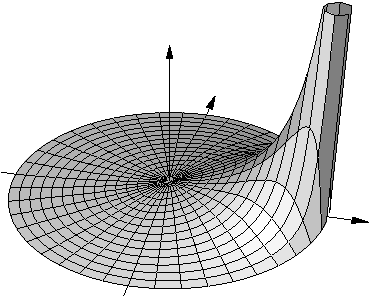
\includegraphics{figures/poisson-graph}
\caption{Grafik kernel Poisson pada $\D$,
kutub di $z=1$ dipotong pada $2$.%
\label{fig:poissongraph}}
\end{myfig}

\begin{prop}\label{prop:Poissonprops}
\leavevmode
\begin{enumerate}[(i)]
\item
$P_r(\theta) > 0$ untuk semua $0 \leq r < 1$ dan semua $\theta$.
\item
$\int_{-\pi}^{\pi} P_r(\theta) \, d\theta = 1$
untuk semua $0 \leq r < 1$.
\item
Untuk setiap $\delta > 0$ yang diberikan,
$\sup \bigl\{P_r(\theta) : \delta \leq \abs{\theta} \leq
\pi \bigr\} \to 0$ ketika $r \uparrow 1$.
\end{enumerate}
\end{prop}

Dalam bukti, berguna untuk memvisualisasikan grafik
$P_r$ sebagai fungsi dari $\theta$ untuk $r$ tetap.
Lihat \figureref{fig:poisson2dgraph}.

\begin{myfig}
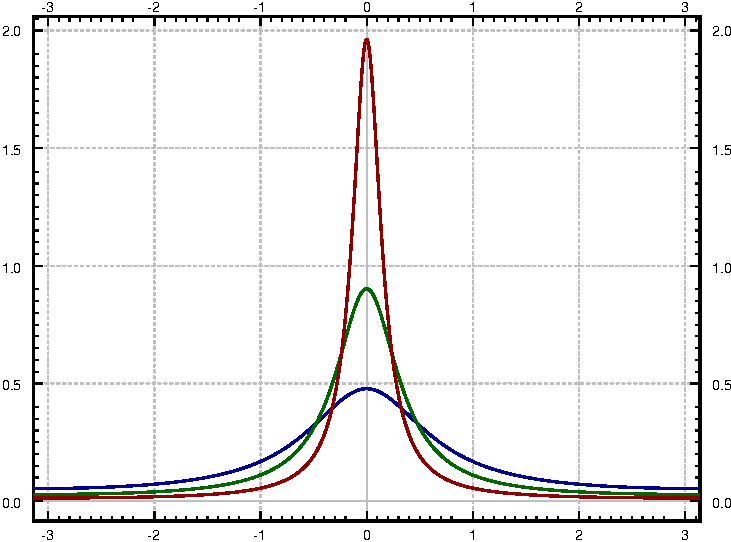
\includegraphics[width=0.5\textwidth]{figures/poisson-kernel.pdf}
\caption{Grafik $P_r$ sebagai fungsi dari $\theta$ pada $[-\pi,\pi]$ untuk
$r=0.5$, $r=0.7$, dan $r=0.85$.\label{fig:poisson2dgraph}}
\end{myfig}

\begin{proof}
Butir pertama mengikuti karena
untuk $0 \leq r < 1$, kita memperoleh
$1-r^2 > 0$
dan
\begin{equation*}
1+r^2-2r \cos\theta \geq 1+r^2-2r = {(1-r)}^2 > 0 .
\end{equation*}

Untuk butir kedua,
\begin{equation*}
\begin{split}
\int_{-\pi}^{\pi}
P_r(\theta) \, d\theta
& =
\frac{1}{2\pi}
\int_{-\pi}^{\pi}
\Re
\left(
\frac{1+re^{i\theta}}{1-re^{i\theta}}
\right)
\, d\theta
\\
& =
\Re
\frac{1}{2\pi i}
\int_{-\pi}^{\pi}
\frac{1+re^{i\theta}}{1-re^{i\theta}} \frac{1}{re^{i\theta}} \,
ire^{i\theta}
\, d\theta
\\
& =
\Re
\frac{1}{2\pi i}
\int_{\partial \Delta_r(0)}
\frac{(1+z)/(1-z)}{z} \, dz
=
\Re \frac{1+0}{1-0} = 1 .
\end{split}
\end{equation*}
Kesamaan pada baris ketiga mengikuti dari rumus integral Cauchy
dengan menggunakan fungsi $\frac{1+z}{1-z}$ yang dievaluasi di $0$.

Untuk butir ketiga, kita hanya perlu membuktikan
hasil tersebut untuk $\delta \leq \theta \leq \pi$ berdasarkan simetri ($P_r$ genap).
Pada $(0,\pi)$, $P_r$ menurun secara ketat karena $\cos \theta$ menurun secara ketat.
Jadi kita hanya perlu menunjukkan bahwa $P_r(\delta)$ menuju $0$
ketika $r \to 1$ jika $\delta > 0$.
Fakta ini mengikuti karena $r \mapsto
\frac{1+re^{i\delta}}{1-re^{i\delta}}$
kontinu di $r=1$ dan
\begin{equation*}
\frac{1+e^{i\delta}}{1-e^{i\delta}}
=
\frac{(1+e^{i\delta})(1-e^{-i\delta})}{(1-e^{i\delta})(1-e^{-i\delta})}
=
\frac{e^{i\delta}-e^{-i\delta}}{\sabs{1-e^{i\delta}}^2}
=
i \frac{2\Im e^{i\delta}}{\sabs{1-e^{i\delta}}^2}
\end{equation*}
bernilai imajiner murni.
\end{proof}

\begin{thm} \label{thm:dirichsol}
Misalkan $f \colon \partial \D \to \R$ kontinu.
Maka
$Pf \colon \overline{\D} \to \R$, yang didefinisikan oleh
\glsadd{not:Pf}%
\begin{equation*}
Pf(re^{i\theta})
=
\begin{cases}
\int_{-\pi}^\pi f(e^{it}) P_{r}(\theta-t) \, dt
&
\text{jika $r < 1$,} \\
f(e^{i\theta}) & \text{jika $r=1$,}
\end{cases}
\end{equation*}
harmonik di $\D$ dan kontinu pada $\overline{\D}$.
\end{thm}

\begin{proof}
Pertama, kita buktikan bahwa $Pf$ harmonik di $\D$. Misalkan $z = re^{i\theta}$.
Maka untuk setiap $t$ tetap,
\begin{equation*}
P_r(\theta-t)
=
\frac{1}{2\pi}
\Re
\left(
\frac{1+re^{i(\theta-t)}}{1-re^{i(\theta-t)}}
\right)
=
\frac{1}{2\pi}
\Re
\left(
\frac{1+ze^{-it}}{1-ze^{-it}}
\right)
\end{equation*}
harmonik sebagai fungsi dari $z=re^{i\theta}$.
Dengan mendiferensialkan di bawah tanda integral,
\begin{equation*}
Pf(z)
=
Pf(re^{i\theta})
=
\int_{-\pi}^\pi f(e^{it}) P_r(\theta-t) \, dt
=
\frac{1}{2\pi}
\int_{-\pi}^\pi f(e^{it})
\Re
\left(
\frac{1+z e^{-it}}{1-z e^{-it}}
\right)
\, dt
\end{equation*}
harmonik di $z = re^{i\theta} \in \D$.

Selanjutnya kita buktikan kekontinuan pada titik-titik di $\partial \D$.
Karena $P_r$ dan $f(e^{it})$ sama-sama $2 \pi$-periodik, kita
mengganti variabel:
\begin{equation*}
Pf(re^{i\theta})
=
\int_{-\pi}^\pi f(e^{it}) P_r(\theta-t) \, dt
=
\int_{-\pi}^\pi f\bigl(e^{i(\theta-t)}\bigr) P_r(t) \, dt .
\end{equation*}
Misalkan $M > 0$ suatu batas atas bagi
$\sabs{f}$ pada $\partial \D$. Misalkan $\epsilon > 0$ diberikan.
Karena $f$ kontinu seragam pada $\partial \D$, pertimbangkan $\delta > 0$
yang cukup kecil sehingga $\babs{f(e^{i(\theta-t)})-f(e^{i\theta})} <
\nicefrac{\epsilon}{2}$ kapan pun $\sabs{t} < \delta$.
\propref{prop:Poissonprops} menyatakan bahwa terdapat
suatu $\delta' > 0$ sedemikian sehingga jika
$1-\delta' < r < 1$, maka
$0 < P_r(t) < \frac{\epsilon}{8M\pi}$
kapan pun $\delta \leq \sabs{t} \leq \pi$.

Karena
$\int_{-\pi}^\pi P_r(t) \, dt = 1$,%
\footnote{Ini merupakan trik yang selalu dijumpai dalam analisis; baik untuk
mengingatnya.}
\begin{equation*}
f(e^{i\theta})=
\int_{-\pi}^\pi f(e^{i\theta}) P_r(t) \, dt .
\end{equation*}
Jadi
\begin{equation*}
\begin{split}
\sabs{
Pf(r e^{i\theta} ) - f(e^{i\theta})
}
& =
\abs{
\int_{-\pi}^{\pi} \bigl( f(e^{i(\theta-t)})-f(e^{i\theta}) \bigr) P_r(t) \, dt
}
\\
& \leq
\abs{
\int_{-\pi}^{-\delta} \cdots \, dt
}
+
\abs{
\int_{-\delta}^{\delta} \cdots \, dt
}
+
\abs{
\int_{\delta}^\pi \cdots \, dt
} .
\end{split}
\end{equation*}
Mari kita estimasi ketiga integral tersebut.
Pertama,
\begin{equation*}
\begin{split}
\abs{
\int_{-\pi}^{-\delta} \bigl( f(e^{i(\theta-t)})-f(e^{i\theta}) \bigr) P_r(t) \, dt
}
& \leq
\int_{-\pi}^{-\delta} \abs{ f(e^{i(\theta-t)})-f(e^{i\theta}) }
P_r(t) \, dt
\\
& \leq (\pi-\delta) 2M \frac{\epsilon}{8M\pi} < \frac{\epsilon}{4} .
\end{split}
\end{equation*}
Integral dari $\delta$ hingga $\pi$ persis sama.
Selanjutnya, integral tengah,
\begin{equation*}
\begin{split}
\abs{
\int_{-\delta}^{\delta} \bigl( f(e^{i(\theta-t)})-f(e^{i\theta}) \bigr) P_r(t) \, dt
}
& \leq
\int_{-\delta}^{\delta} \abs{f(e^{i(\theta-t)})-f(e^{i\theta})}
P_r(t) \, dt
\\
& \leq
\int_{-\delta}^{\delta} \frac{\epsilon}{2} P_r(t) \, dt
\leq
\int_{-\pi}^{\pi} \frac{\epsilon}{2} P_r(t) \, dt
=\frac{\epsilon}{2} .
\end{split}
\end{equation*}
Dengan menggabungkan semuanya, selama $1-\delta' < r < 1$,
\begin{equation*}
\sabs{
Pf(r e^{i\theta} ) - f(e^{i\theta})
} < \frac{\epsilon}{4} + \frac{\epsilon}{2} + \frac{\epsilon}{4} =
\epsilon.
\end{equation*}
Jadi $Pf(re^{i\theta}) \to f(e^{i\theta})$ secara seragam dalam $\theta$
ketika $r \uparrow 1$.
Keseragaman ini penting di bawah.

Terakhir, untuk setiap $z_0 = e^{i\theta_0} \in \partial \D$,
kita harus menunjukkan bahwa
$Pf(z)$ menuju $Pf(z_0)=f(z_0)$ ketika $z \in \overline{\D}$ menuju $z_0$.
Misalkan $\epsilon > 0$ diberikan. Karena $f = Pf|_{\partial \D}$
kontinu, pilih suatu $\delta > 0$ sedemikian sehingga
$\babs{Pf(e^{i\theta})-Pf(e^{i\theta_0})} < \nicefrac{\epsilon}{2}$
kapan pun $\sabs{\theta-\theta_0} < \delta$.
Kecilkan pula $\delta$ secukupnya sehingga
$\babs{Pf(re^{i \theta})-Pf(e^{i\theta})} < \nicefrac{\epsilon}{2}$
ketika $1 - \delta < r \leq 1$ untuk semua $\theta$.
Dengan menggabungkan kedua estimasi, kita memperoleh
\begin{equation*}
\babs{Pf(re^{i\theta})-Pf(e^{i\theta_0})}
\leq
\babs{Pf(re^{i\theta})-Pf(e^{i\theta})}
+
\babs{Pf(e^{i\theta})-Pf(e^{i\theta_0})}
< \epsilon
\end{equation*}
kapan pun $z=re^{i\theta}$ memenuhi $1 - \delta < r \leq 1$ dan
$\sabs{\theta-\theta_0} < \delta$.
Lihat \figureref{fig:proofofdirichlet}.
Oleh karena itu, $Pf$
kontinu di $z_0$.
\begin{myfig}
\subimport*{figures/}{proofofdirichlet.pdf_t}
\caption{Kekontinuan $Pf$ di $z_0$.\label{fig:proofofdirichlet}}
\end{myfig}
\end{proof}

Kita catat bahwa dalam bukti tersebut kita menggunakan topologi pada $\overline{\D}$
yang diberikan oleh koordinat polar, dan kita mengestimasi koordinat-koordinatnya secara terpisah.
Koordinat polar memberikan homeomorfisme lokal yang baik
(suatu pemetaan bijektif kontinu dengan invers kontinu) di luar
titik asal, yang memadai bagi kita karena kita hanya memperhatikan titik-titik
pada atau dekat batas $\D$. Pembaca yang masih belum yakin
hendaknya menuliskan rinciannya sebagai latihan.

\begin{exbox}
\begin{exercise}
Kita telah membuktikan bahwa untuk setiap $\epsilon > 0$, terdapat suatu $\delta > 0$ sedemikian sehingga
$\babs{Pf(re^{i\theta})-Pf(e^{i\theta_0})} < \epsilon$
ketika $\sabs{\theta-\theta_0} < \delta$ dan
$1 - \delta < r \leq 1$. Buktikan bahwa pernyataan ini sungguh berarti bahwa
$\lim_{z \to z_0} Pf(z) = f(z_0) = Pf(z_0)$.
\end{exercise}
\end{exbox}

Translasi dan penskalaan memberikan versi yang lebih umum untuk
sebarang cakram.

\begin{cor} \label{cor:dirichsol}
Misalkan $f \colon \partial \Delta_R(p) \to \R$ kontinu.
Maka
$Pf \colon \overline{\Delta_R(p)} \to \R$, yang didefinisikan oleh
\glsadd{not:Pf}%
\begin{equation*}
Pf(p + re^{i\theta})
=
\begin{cases}
\int_{-\pi}^\pi f(p+Re^{it}) P_{r/R}(\theta-t) \, dt
&
\text{jika $r < R$,} \\
f(p+Re^{i\theta}) & \text{jika $r=R$,}
\end{cases}
\avoidbreak
\end{equation*}
harmonik di $\Delta_R(p)$ dan kontinu pada $\overline{\Delta_R(p)}$.
\end{cor}

\begin{exbox}
\begin{exercise}
Buktikan korolari tersebut.
\end{exercise}
\end{exbox}

Karena integral Poisson memberikan suatu solusi bagi masalah Dirichlet pada cakram,
dan karena solusi masalah Dirichlet unik,
integral Poisson memberikan
suatu representasi fungsi harmonik dalam suku-suku nilai batas, tepat
seperti yang diberikan rumus integral Cauchy bagi fungsi holomorfik.
Artinya, jika $\overline{\Delta_R(p)} \subset U$ dan $f$ harmonik di $U$,
maka $P[f|_{\partial \Delta_R(p)}] = f|_{\overline{\Delta_R(p)}}$.
Secara khusus, untuk $z = p+re^{i\theta} \in \Delta_R(p)$,
\begin{equation*}
f(z) = \int_{-\pi}^\pi f(p+Re^{it}) P_{r/R}(\theta-t) \, dt .
\end{equation*}
Perbedaannya dengan rumus integral Cauchy ialah bahwa kernel Poisson
berubah sesuai domainnya. Kernel Poisson tersedia bagi
domain selain cakram (asalkan batasnya cukup baik), meskipun
secara umum kita tidak mempunyai rumus eksplisit. Dalam
rumus integral Cauchy, kernelnya adalah $\frac{1}{\zeta-z}$
apa pun lintasan yang kita integralkan, yakni, apa pun
domain tempat kita menyelesaikan persoalan.

Kernel Poisson juga merupakan kernel reproduksi bagi
fungsi holomorfik, karena fungsi holomorfik bersifat harmonik
(bagian real dan imajinernya demikian). Jika $f$ memberikan nilai-nilai batas
bagi suatu fungsi holomorfik, maka $Pf$ holomorfik dan sama dengan
transformasi Cauchy $Cf$ di dalam cakram. Namun, tidak seperti
transformasi Cauchy, $Pf$ selalu kontinu hingga ke batas jika diberikan data
kontinu pada cakram. Jadi, jika $f$ bukan nilai batas dari
suatu fungsi holomorfik, $Cf$ dan $Pf$ berbeda di dalam cakram.
Sebagai contoh, jika $f=z+\bar{z}$ pada lingkaran, maka $Pf = z+\bar{z}$ di $\D$
tetapi $Cf = z$ di $\D$.

%Kernel Poisson juga tersedia untuk dimensi yang lebih tinggi, yakni, di $\R^n$ untuk
%$n > 2$, dan mempunyai
%sifat-sifat analog, meskipun kita tidak akan mempelajarinya di sini.

Sangat berguna untuk memperhatikan bahwa
dalam korolari, jika kita menyubstitusikan $r=0$, kita memperoleh
\begin{equation} \label{eq:averageofPf}
Pf(p) = \frac{1}{2\pi} \int_{-\pi}^{\pi}f(p + R e^{it}) \, dt .
\end{equation}
Nilai di pusat cakram, $Pf(p)$, merupakan nilai
rata-rata dari $f$ pada $\partial \Delta_R(p)$.
Dalam bagian berikutnya, kita akan melihat bahwa sifat ini sesungguhnya mengarakterisasi
fungsi harmonik.

\begin{exbox}
\begin{exercise}[Mudah]
Buktikan bahwa untuk setiap $f \colon \partial \D \to \C$ yang kontinu,
terdapat suatu $F \colon \D \to \C$ yang holomorfik sedemikian sehingga $\Re F$ dapat diperluas
secara kontinu ke $\overline{\D}$ (sama dengan suatu fungsi kontinu pada
$\overline{\D}$) dan sedemikian sehingga $\Re F = \Re f$ pada $\partial \D$.
Artinya, dengan diberikan data batas sebarang, secara umum kita tidak dapat menemukan suatu
fungsi holomorfik dengan nilai-nilai batas tersebut, tetapi setidaknya kita dapat melakukannya
untuk bagian real.
\end{exercise}

\begin{exercise} \label{exercise:dirichDwithsings}
Nyatakan dan buktikan suatu versi dari \thmref{thm:dirichsol} untuk fungsi yang
terbatas pada $\partial \D$ dan kontinu di semua kecuali berhingga banyak titik pada
$\partial \D$. Tentu saja kesimpulannya haruslah bahwa $Pf(z)$ ($z \in
\D$) menuju
$f(z_0)$ ($z_0 \in \partial \D$) hanya jika $f$ kontinu di $z_0$.
Catatan: Mahasiswa yang lebih lanjut hendaknya mencatat bahwa keterbatasan tidak diperlukan,
cukup $f \in L^1(\partial \D)$.
\end{exercise}

\begin{exercise} \label{exercise:upperhalfplanedirichlet}
Masalah Dirichlet pada setengah bidang atas $\bH = \{ z \in \C : \Im z > 0 \}$
tidak mempunyai solusi unik. Petunjuk: Temukan dua
fungsi harmonik berbeda yang bernilai nol pada $\R$.
\end{exercise}

\begin{exercise}
\pagebreak[2]
Diberikan suatu $f \colon \R \to \R$ yang terbatas dan kontinu, buktikan bahwa
$Pf \colon \overline{\bH} \to \R$,
\begin{equation*}
Pf(x+iy)
=
\begin{cases}
\frac{1}{\pi}
\int_{-\infty}^{\infty} f(t) \frac{y}{{(x-t)}^2+y^2} \, dt
&
\text{jika $y > 0$,} \\
f(x) & \text{jika $y=0$,}
\end{cases}
\end{equation*}
harmonik di $\bH$ dan kontinu pada $\overline{\bH}$.
\end{exercise}

\begin{exercise}\label{exercise:martinfunctions}
Diberikan suatu himpunan terbuka $U \subset \C$,
suatu fungsi kontinu $f \colon \widebar{U} \to \R$,
yang positif dan harmonik pada $U$,
serta bernilai nol pada $\partial U$, fungsi itu disebut
\emph{\myindex{fungsi Martin}}.
\begin{exparts}
\item
Temukan suatu fungsi Martin pada setengah bidang atas $\bH$.
\item
Temukan suatu fungsi Martin pada $\{ z \in \C : \Re z > 0, 0 < \Im z < 1
\}$. Petunjuk: Sinus hiperbolik.
\item
Buktikan bahwa jika $U$ terbatas, maka tidak terdapat fungsi Martin pada $U$.
\end{exparts}
\end{exercise}

\begin{exercise}
Selesaikan secara eksplisit masalah Dirichlet berikut: Misalkan $0 < r < R$ dan $a,b
\in \R$ diberikan. Temukan suatu $f \colon \overline{\ann(0;r,R)} \to
\R$ yang kontinu, harmonik pada $\ann(0;r,R)$, sedemikian sehingga $f=a$ pada $\sabs{z}=r$ dan $f=b$
pada $\sabs{z}=R$.
\end{exercise}

\begin{exercise}
Turunkan \emph{\myindex{rumus integral Schwarz}}, yang merekonstruksi
suatu fungsi holomorfik dari bagian real nilai-nilai batas
dan nilai bagian imajiner di satu titik.
Jika $f \colon \overline{\D} \to \C$ kontinu dan holomorfik pada
$\D$, maka untuk semua $z \in \D$,
\begin{equation*}
f(z) =
\frac{1}{2\pi i}
\int_{\partial \D}
\frac{\zeta+z}{\zeta-z} \frac{\Re f(\zeta)}{\zeta} \, d\zeta
+ i \Im f(0) .
\end{equation*}
\end{exercise}

\begin{exercise}
Misalkan $q_1,q_2,\ldots$ suatu enumerasi dari bilangan-bilangan
rasional di $[0,1]$.
\begin{exparts}
\item
Definisikan $\varphi \colon [0,1] \to {\mathbb R}$
melalui $\varphi(t) = \sum_{j=1}^\infty 2^{-j} \chi_{[q_j,1]}(t)$,
dengan $\chi_{[q_j,1]}(t) = 1$ jika $t \in [q_j,1]$ dan
nol jika tidak (fungsi indikator). Tunjukkan bahwa
$\varphi$ diskontinu di setiap bilangan rasional dalam $(0,1]$,
takmenurun, dan terbatas (sehingga terintegralkan Riemann).
\item
Definisikan $\Phi(t) = \int_0^t \varphi(s)\, ds$, tunjukkan bahwa $\Phi$
meningkat, kontinu, tetapi tidak terdiferensialkan
pada suatu himpunan padat di $[0,1]$. Gunakan fungsi itu untuk membangun suatu
$\psi(t)$ yang $2\pi$-periodik, kontinu, dan
tidak terdiferensialkan pada suatu subhimpunan padat dari $\R$.
\item
Temukan suatu $u \colon \overline{\D} \to \R$ yang kontinu
sedemikian sehingga $u|_{\D}$ harmonik dan
$u(e^{it}) = \psi(t)$, kemudian temukan suatu $h \colon \D \to \C$ yang holomorfik
sedemikian sehingga $\Re h = u$.
\item
Tunjukkan bahwa $h$ tidak dapat diperluas melewati titik mana pun dari
batas, yakni, untuk setiap
$z_0 \in \partial \D$ dan setiap lingkungan terbuka
$U$ dari $z_0$, tidak terdapat suatu $f \colon U \to \C$ yang holomorfik
sedemikian sehingga $f = h$ pada $\D \cap U$.
\end{exparts}
\end{exercise}
\end{exbox}

\subsection{Sifat nilai rata-rata}

Kita dapat mendefinisikan fungsi harmonik dalam satu variabel real
dengan menyatakan bahwa $f$ harmonik jika
$\nabla^2 f = \frac{\partial^2}{\partial x^2} f = f'' = 0$, yakni, $f(x) = Ax+B$, suatu fungsi
linear afin. Cukup berguna untuk memandang fungsi harmonik pada $\C$ sebagai satu
analog khusus dari fungsi linear afin semacam itu, meskipun tentu saja analogi ini
tidak boleh dibawa terlalu jauh.
Salah satu sifat fungsi linear afin ialah sifat nilai rata-rata, yakni,
jika $a < b$ diberikan maka $f\bigl(\frac{a+b}{2}\bigr) = \frac{f(a)+f(b)}{2}$. Nilai
di pusat suatu interval sama dengan rata-rata nilai pada
ujung-ujungnya. Sesungguhnya, jika suatu fungsi kontinu memenuhi kesamaan ini untuk semua
interval $[a,b]$, maka fungsi itu
linear afin (latihan). Sifat nilai rata-rata ini sepenuhnya mengarakterisasi fungsi
linear afin (yakni, harmonik) di $\R$.
Cukup menarik bahwa sifat sejenis juga mengarakterisasi
fungsi harmonik di $\C$, meskipun kita harus mengganti suatu interval
dengan suatu cakram.

\begin{thm}[Sifat nilai rata-rata]\label{thm:meanprop}\index{sifat nilai rata-rata}
\pagebreak[0]
Misalkan $U \subset \C$ terbuka.
Suatu fungsi kontinu
$f \colon U \to \R$
harmonik jika dan hanya jika untuk setiap $p \in U$, terdapat suatu $R_p >0$
sedemikian sehingga $\Delta_{R_p}(p) \subset U$ dan
\begin{equation*}
f(p) = \frac{1}{2\pi} \int_{-\pi}^{\pi} f(p+re^{i\theta})\, d\theta
\qquad \text{untuk semua } r < R_p .
\avoidbreak
\end{equation*}
Lebih lanjut, jika $f$ harmonik, maka kita dapat memilih sebarang
$R_p > 0$ sedemikian sehingga $\Delta_{R_p}(p) \subset U$.
\end{thm}

\begin{proof}
Satu arah (dan bagian \myquote{Lebih lanjut}) mengikuti dengan cepat.
Misalkan $f$ harmonik.
Ambil $p \in U$ dan
sebarang $R_p > 0$ sedemikian sehingga $\Delta_{R_p}(p) \subset U$.
Untuk setiap $r < R_p$,
selesaikan masalah Dirichlet di $\Delta_r(p)$ menggunakan kernel Poisson
dengan nilai-nilai batas
$f|_{\partial \Delta_r(p)}$. Dengan menggunakan \eqref{eq:averageofPf} dan
keunikan solusi masalah Dirichlet, kita memperoleh
\begin{equation*}
f(p) = P\bigl[f|_{\partial \Delta_r(p)}\big](p) =
\frac{1}{2\pi} \int_{-\pi}^{\pi}f(p + r e^{it}) \, dt .
\end{equation*}

Sebaliknya, misalkan $f$ kontinu dan memenuhi
sifat nilai rata-rata untuk semua $p$ dan semua $r < R_p$.
Misalkan $\overline{\Delta_s(q)} \subset U$ suatu
cakram tertutup sebarang. Misalkan $h = P\bigl[f|_{\partial \Delta_s(q)}\big]$
adalah solusi masalah Dirichlet di $\Delta_s(q)$ dengan nilai-nilai batas
yang diberikan oleh $f$. Pertimbangkan $\varphi = f-h$,
yang kontinu, bernilai nol secara identik
pada $\partial \Delta_s(q)$, dan memenuhi sifat nilai rata-rata
pada lingkaran-lingkaran yang sama dengan $f$ (selama lingkaran itu terletak dalam $\Delta_s(q)$).
Andaikan demi kontradiksi bahwa $\varphi$ positif
di suatu tempat pada $\Delta_s(q)$.
Misalkan $\varphi$ mencapai suatu maksimum di $p \in
\Delta_s(q)$, sehingga $\varphi(p) > 0$.
Himpunan $X \subset \Delta_s(q)$ tempat $\varphi(z) = \varphi(p)$ bersifat kompak.
Asumsikan $p$ adalah titik pada $X$ yang paling dekat dengan
$\partial \Delta_s(q)$. Untuk suatu $r < R_p$ yang kecil, lingkaran
$\partial \Delta_r(p) \subset \Delta_s(q)$ dan terdapat suatu konstanta
$C$ sedemikian sehingga $\varphi(z) \leq C < \varphi(p)$ untuk $z$
pada suatu subhimpunan terbuka takkosong
dari $\partial \Delta_r(p)$. Lihat \figureref{fig:meanvalue}.
Secara khusus, karena
$\varphi$ seharusnya memenuhi
sifat nilai rata-rata pada $\Delta_r(p)$, kita memperoleh kontradiksi
\begin{equation*}
\frac{1}{2\pi} \int_{-\pi}^{\pi} \varphi(p+re^{i\theta})\, d\theta <
\varphi(p) .
\end{equation*}

\begin{myfig}
%Perhatikan bahwa gambar ini juga digunakan kemudian
\subimport*{figures/}{meanvalue.pdf_t}
\caption{Cakram-cakram $\Delta_s(q)$ dan $\Delta_r(p)$ serta himpunan
$X$.\label{fig:meanvalue}}
\end{myfig}

Kita telah membuktikan bahwa $\varphi \leq 0$ pada $\Delta_s(q)$. Dengan menerapkan
logika yang sama pada $-\varphi$, kita memperoleh bahwa $\varphi = 0$ pada $\Delta_s(q)$.
Dengan kata lain, $f=h$ dan $h$ harmonik, sehingga $f$ harmonik pada
$\Delta_s(q)$ (dan dengan demikian pada $U$).
\end{proof}

Salah satu akibat langsung dari sifat nilai rata-rata adalah bahwa limit
fungsi-fungsi harmonik yang seragam pada himpunan bagian kompak bersifat harmonik.  Sama seperti untuk
fungsi holomorfik, hasil ini akan sulit dibuktikan dengan menggunakan definisi
fungsi harmonik.  Diberikan barisan $\{ f_n \}$ dari sembarang fungsi $C^2$
dengan limit seragam $f$,
limit dari $\nabla^2 f_n$ belum tentu
$\nabla^2 f$.  Akan tetapi,
limit seragam dapat dilewatkan ke dalam integral.  Hasil berikut merupakan salah satu bagian
dari apa yang disebut \emph{\myindex{teorema pertama Harnack}} (beberapa
hasil tentang fungsi harmonik dinamai menurut Harnack).

\begin{thm}[Teorema pertama Harnack]\label{thm:harnack1}
Misalkan $U \subset \C$ terbuka, dan misalkan $f_n \colon U \to \R$ suatu barisan
fungsi harmonik yang konvergen secara seragam pada himpunan bagian kompak ke $f \colon U
\to \R$.  Maka $f$ harmonik.
\end{thm}

\begin{proof}
Pertama, $f$ kontinu.
Diberikan sembarang cakram $\overline{\Delta_r(p)} \subset U$,
barisan $\{ f_n \}$ konvergen secara seragam pada batas cakram
dan di $p$, sehingga
\begin{equation*}
f(p) =
\lim_{n\to\infty} f_n(p)
=
\lim_{n\to\infty} 
\frac{1}{2\pi} \int_{-\pi}^{\pi} f_n(p+re^{i\theta})\, d\theta
=
\frac{1}{2\pi} \int_{-\pi}^{\pi} f(p+re^{i\theta})\, d\theta .
\end{equation*}
Hasilnya mengikuti dari sifat nilai rata-rata.
\end{proof}

\begin{exbox}
\begin{exercise}
Misalkan $f \colon \R \to \R$ fungsi kontinu sedemikian sehingga
$f\bigl(\frac{a+b}{2}\bigr) = \frac{f(a)+f(b)}{2}$ kapan pun $a < b$.
Buktikan bahwa $f(x) = Ax + B$ untuk suatu konstanta $A,B$.
\end{exercise}

\begin{exercise}
Buktikan prinsip maksimum untuk fungsi harmonik secara langsung dari
sifat nilai rata-rata.
\end{exercise}

\begin{exercise}
Misalkan $U \subset \C$ terbuka, $f \colon U \to \R$ kontinu, $p \in U$,
dan $f$ harmonik pada $U \setminus \{ p \}$.  Buktikan bahwa $f$ sebenarnya
harmonik pada seluruh $U$.
\end{exercise}

\begin{exercise}
Misalkan $f$ harmonik di suatu lingkungan dari
$\overline{\Delta_r(0)}$ dan
$f(0) = 0$.  Buktikan bahwa
\begin{equation*}
\frac{1}{2} \int_{-\pi}^\pi \abs{f(re^{it})} \, dt = 
\int_{-\pi}^\pi \max \{ f(re^{it}), 0 \} \, dt .
\end{equation*}
\end{exercise}

\begin{exercise}
Misalkan $f$ harmonik di suatu lingkungan dari
$\overline{\D}$, $f(0) = 0$, dan $\int_{-\pi}^\pi \abs{f(e^{it})}\, dt =
4\pi$.
Buktikan bahwa terdapat $t$ sedemikian sehingga $f(e^{it}) = 1$ dan $s$ sedemikian sehingga
$f(e^{is}) = -1$.
\end{exercise}

\begin{exercise}
Misalkan $U \subset \C$ terbuka dan
$f \colon U \times [0,1] \to \R$ kontinu
sedemikian sehingga untuk setiap $t \in [0,1]$ yang tetap, $z \mapsto f(z,t)$ harmonik.
Buktikan bahwa $g \colon U \to \R$ yang didefinisikan oleh
\begin{equation*}
g(z) = \int_0^1 f(z,t) \, dt
\avoidbreak
\end{equation*}
bersifat harmonik.  Petunjuk: Fubini, bukan Leibniz.
\end{exercise}

\begin{exercise}
Misalkan $U \subset \C$ terbuka.
Buktikan bahwa fungsi kontinu $f \colon U \to \R$
harmonik jika dan hanya jika memenuhi
\emph{\myindex{sifat nilai rata-rata cakram}} untuk setiap $\overline{\Delta_r(p)}
\subset U$:
\begin{equation*}
f(p) = 
\frac{1}{\pi r^2} \int_{\overline{\Delta_r(p)}} f(z) \, dA.
\end{equation*}
\end{exercise}

\begin{exercise}
Dengan sedikit kehati-hatian,
tidak perlu mengasumsikan sifat nilai rata-rata untuk semua cakram yang cukup kecil.
Misalkan $f \colon \overline{\D} \to \R$
kontinu dan sedemikian sehingga untuk setiap $p \in \D$, terdapat $r$ sehingga
$\overline{\Delta_r(p)} \subset \D$ dan 
\begin{equation*}
f(p) = \frac{1}{2\pi} \int_{-\pi}^{\pi} f(p+re^{i\theta})\, d\theta .
\end{equation*}
Buktikan bahwa $f$ harmonik di $\D$.
\end{exercise}
\end{exbox}

\subsection{Ketaksamaan Harnack}

Seperti fungsi holomorfik, fungsi harmonik yang didefinisikan pada suatu
cakram tidak dapat bertingkah sesuka hati di dalam cakram tersebut.  Perilakunya
sampai batas tertentu dikendalikan oleh ukuran cakram: Semakin jauh cakram itu berada
\myquote{di dalam} ranah definisinya, semakin besar kendali yang kita miliki.
Pernyataan dasar kendali ini adalah
\emph{ketaksamaan Harnack}\index{ketaksamaan Harnack!cakram} pada cakram.
Untuk fungsi holomorfik, hasil yang analog adalah
\hyperref[lemma:schwarz]{lemma Schwarz}, di mana kita
mensyaratkan fungsi-fungsinya terbatas (nilainya berada dalam suatu cakram).  Untuk fungsi
harmonik, analog dari keterbatasan adalah kenegatifan-nol.

\begin{thm}[Ketaksamaan Harnack]
\label{thm:harnackineqdisc}
Misalkan $f \colon \Delta_R(p) \to \R$ harmonik dan taknegatif,
dan misalkan $0 < r < R$.
Maka untuk semua $z \in \overline{\Delta_r(p)}$,
\begin{equation*}
\frac{R-r}{R+r} f(p) \leq f(z) \leq \frac{R+r}{R-r} f(p) .
\end{equation*}
\end{thm}

\begin{proof}
Jika kita membuktikan ketaksamaan untuk $z$ pada 
$\partial \Delta_r(p)$, yaitu, $\sabs{z-p}=r$, maka kita selesai
karena $\frac{R+r}{R-r}$ naik terhadap $r$ dan
$\frac{R-r}{R+r}$ turun terhadap $r$.  Jadi 
anggap $z = p+re^{i\theta}$.

Misalkan $S$ sedemikian sehingga $0 < r < S < R$.
Dengan menggunakan \corref{cor:dirichsol} dan keunikan
solusi masalah
Dirichlet,
\begin{multline*}
f(z)
=
f(p + re^{i\theta})
=
\int_{-\pi}^\pi f(p+Se^{it}) P_{r/S}(\theta-t) \, dt
\\
=
\frac{1}{2\pi} 
\int_{-\pi}^\pi f(p+Se^{it})
\frac{S^2-r^2}{S^2+r^2-2Sr \cos (\theta-t)}
\, dt .
\end{multline*}
Kita menaksir
\begin{equation*}
\frac{S-r}{S+r}
=
\frac{S^2-r^2}{S^2+r^2+2Sr}
\leq
\frac{S^2-r^2}{S^2+r^2-2Sr \cos (\theta-t)}
\leq
\frac{S^2-r^2}{S^2+r^2-2Sr}
=
\frac{S+r}{S-r} .
\end{equation*}
Untuk $z = p+re^{i\theta}$,
dengan menggunakan bahwa $f$ taknegatif,
\begin{equation*}
f(z)
=
\int_{-\pi}^\pi f(p+Se^{it}) P_{r/S}(\theta-t) \, dt
\leq
\frac{S+r}{S-r} 
\left(
\frac{1}{2\pi}
\int_{-\pi}^\pi f(p+Se^{it}) \, dt
\right)
=
\frac{S+r}{S-r} 
f(p) .
\end{equation*}
Ketaksamaan bawah mengikuti dengan cara yang sama.
Karena $S<R$ sebarang, ketaksamaan dalam teorema 
mengikuti dengan mengambil limit.
\end{proof}

Ketaksamaan-ketaksamaan ini optimal.  Pada cakram satuan $\D$, teorema tersebut menyatakan
\begin{equation*}
\frac{1-r}{1+r} f(0) \leq f(z) \leq \frac{1+r}{1-r} f(0) .
\end{equation*}
Perhatikan fungsi $f(z) = \Re \frac{1+z}{1-z}$.  Selain faktor
$\frac{1}{2\pi}$, fungsi ini adalah kernel Poisson, sehingga 
$f(z) > 0$ pada $\D$.  Perhatikan bahwa $f(0)=1$.  Dengan menyubstitusikan $z=r$, kita memperoleh
kesamaan pada ketaksamaan ruas kanan di atas, dan dengan menyubstitusikan $z=-r$
kita memperoleh kesamaan pada ketaksamaan ruas kiri di atas.  Dengan kata lain,
kedua konstanta
$\frac{R-r}{R+r}$ dan $\frac{R+r}{R-r}$ adalah optimal.

Ada pula versi umum ketaksamaan Harnack pada sebarang ranah.

\begin{cor}[Ketaksamaan Harnack]\index{ketaksamaan Harnack!sebarang ranah}
Misalkan $U \subset \C$ ranah dan $K \subset U$ kompak.
Maka terdapat $C > 0$ sedemikian sehingga
\begin{equation*}
\sup_{z \in K} f(z) \leq C \inf_{z\in K} f(z)
\end{equation*}
untuk setiap fungsi harmonik taknegatif $f$ yang didefinisikan pada $U$.
\end{cor}

\begin{proof}
Jika kita membuktikan teorema untuk $K$ yang lebih besar, kita selesai, jadi kita
mengganti $K$ dengan himpunan bagian kompak terhubung yang lebih besar dari $U$.
Pertama, jadikan $K$ hanya memiliki berhingga banyak komponen dengan menggantinya
dengan berhingga banyak cakram tertutup
(lihat bukti \lemmaref{lemma:patharoundK}).  Kemudian, $U$ terhubung lintasan,
sehingga dengan menambahkan berhingga banyak lintasan ke $K$, kita dapat menghubungkan
cakram-cakram tersebut.

Misalkan $r> 0$ kurang dari setengah jarak $K$ ke $\partial U$.
Terdapat $N$ cakram $\Delta_{r}(z_1),\ldots,\Delta_{r}(z_N)$ yang menutupi $K$,
dengan $z_j \in K$, sehingga $\Delta_{2r}(z_j) \subset U$ untuk setiap $j$.
Tetapkan $\zeta,\xi \in K$.  Setelah memberi label ulang pada cakram-cakram tersebut,
$\zeta \in \Delta_{r}\bigl(z_{1}\bigr)$
dan
$\xi \in \Delta_{r}\bigl(z_{n}\bigr)$ untuk suatu $n \leq N$.
Karena $K$ terhubung, kita juga mengatur agar
$\Delta_{r}\bigl(z_{j}\bigr) \cap \Delta_{r}\bigl(z_{j+1}\bigr)$
tak kosong untuk semua $j=1,\ldots,n-1$.
Tidak semua cakram harus digunakan.
Bukti ini diilustrasikan dalam \figureref{fig:harnacksgeneral}.

\begin{myfig}
\subimport*{figures/}{harnacksgeneral.pdf_t}
\caption{Rantai cakram dengan pusat $z_1,z_2,z_3,z_4$ yang menghubungkan
$\zeta$ ke $\xi$ di dalam $K$ (ditandai dengan arsiran lebih gelap).  Titik tengah ruas
antara $z_j$ dan $z_{j+1}$ juga ditandai.
Lingkaran penuh adalah cakram berjari-jari $r$, sedangkan
lingkaran putus-putus adalah cakram berjari-jari $2r$.\label{fig:harnacksgeneral}}
\end{myfig}

Misalkan $f$ suatu fungsi harmonik taknegatif sebarang pada $U$.
Untuk sebarang $j$, karena $\Delta_{2r}(z_j) \subset U$, jika kita mengambil sebarang $w \in
\Delta_r(z_j)$, kita peroleh bahwa 
\begin{equation*}
\frac{1}{3} f(z_j) = 
\frac{2r-r}{2r+r} f(z_j)
\leq
f(w)
\leq \frac{2r+r}{2r-r} f(z_j)
= 3 f(z_j) .
\end{equation*}
Dengan kata lain, $f(w) \leq 3 f(z_j)$ dan $f(z_j) \leq 3 f(w)$.

Sekarang kita mengikuti rantai cakram tersebut.
Pertama, karena $\zeta \in \Delta_r(z_1)$, kita memperoleh 
\begin{equation*}
f(\zeta) \leq 3 f(z_1).
\end{equation*}
Kedua, misalkan
$q$ titik tengah antara $z_{j}$ dan $z_{j+1}$.
%Titik $q$ mungkin tidak berada di $K$, tetapi $z_j$ berada di sana, demikian pula $z_{j+1}$.
Geometri sederhana menyatakan bahwa
$q \in \Delta_{r}\bigl(z_{j}\bigr) \cap \Delta_{r}\bigl(z_{j+1}\bigr)$.
Dengan demikian,
\begin{equation*}
f(z_j) \leq 3 f(q) \leq 3 \bigl( 3 f(z_{j+1}) \bigr) = 3^2 f(z_{j+1}).
\end{equation*}
Ketiga, karena $\xi \in \Delta_r(z_n)$, kita memperoleh 
\begin{equation*}
f(z_n) \leq 3 f(\xi).
\end{equation*}
Secara keseluruhan,
\begin{equation*}
f(\zeta) \leq
3^{2n}
f(\xi)
\leq
3^{2N}
f(\xi) .
\end{equation*}
Bilangan $N$ hanya bergantung pada $K$, bukan pada $\zeta$, $\xi$, atau $f$.
Karena $\zeta$ dan $\xi$ sebarang, teorema tersebut terbukti.
\end{proof}

Konstanta yang kita peroleh dalam bukti tidak optimal, tetapi bersifat eksplisit.
Dengan mengasumsikan $K$ terhubung,
kita dapat menghitung $C$ tertentu dengan mengetahui jarak dari $K$
ke batas dan banyaknya cakram berjari-jari $r$ yang diperlukan untuk menutupi $K$.

\begin{exbox}
\begin{exercise}[Mudah]
Tunjukkan dengan contoh bahwa ketaksamaan Harnack umum tidak harus berlaku jika $U$
tidak diasumsikan terhubung.
\end{exercise}

\begin{exercise}[Mudah]
Temukan contoh tandingan berikut terhadap ketaksamaan Harnack
jika $f$ tidak diasumsikan
taknegatif.  Untuk setiap $M > 0$, temukan
fungsi harmonik $f \colon \D \to \R$ sedemikian sehingga $f(0) = 1$ dan
$f(\nicefrac{1}{2}) \geq M$.
\end{exercise}

\begin{exercise}
Tetapkan suatu $s > t > 0$.
Misalkan $U = \{z \in \C : -s < \Re z < s, -1 < \Im z < 1 \}$.
Hitung konstanta eksplisit $C$
(tidak harus optimal)
untuk $K$ berikut dalam
ketaksamaan Harnack umum:
\smallskip
\begin{expartshor}{2}
\item
$K = [-t,t]$.
\item
$K = \{-t,t\}$.
\end{expartshor}
\end{exercise}

\begin{exercise}
Fungsi linear afin $Ax+B$ merupakan versi satu-variabel-real
dari fungsi harmonik.  Nyatakan dan buktikan ketaksamaan Harnack
(analog dari \thmref{thm:harnackineqdisc})
dalam konteks linear afin untuk suatu interval $[a,b]$, bukan suatu cakram.
Temukan konstanta optimal dalam kedua ketaksamaan tersebut seperti yang kita peroleh untuk cakram,
dan buktikan bahwa konstanta-konstanta itu optimal.
\end{exercise}

\begin{exercise}
Misalkan $U = \D$ dan $K=\overline{\Delta_r(0)}$, $r < 1$, dalam 
ketaksamaan Harnack umum.  Buktikan bahwa $C$ dari teorema tersebut
harus menuju tak hingga ketika $r \uparrow 1$.
\end{exercise}

\begin{exercise}
Gunakan ketaksamaan Harnack untuk membuktikan teorema Liouville
untuk fungsi harmonik:\index{teorema Liouville!fungsi harmonik}
Jika $f \colon \C \to \R$ harmonik
dan taknegatif, maka $f$ konstan.
\end{exercise}
\end{exbox}

\subsection{Prinsip Harnack}

Ketaksamaan Harnack mengakibatkan bahwa barisan naik 
fungsi harmonik konvergen ke fungsi harmonik.
Teorema ini disebut dengan berbagai nama,
yaitu prinsip Harnack atau teorema kedua Harnack.

\begin{thm}[Prinsip Harnack]
\index{prinsip Harnack}
\index{teorema kedua Harnack}
Misalkan $U \subset \C$ suatu ranah dan $\{ f_n \}$ barisan
fungsi harmonik pada $U$ sedemikian sehingga $f_1 \leq f_2 \leq f_3 \leq \cdots$.
Maka, $f_n \to +\infty$ secara seragam pada himpunan bagian kompak, atau
$f_n \to f$ untuk suatu fungsi harmonik $f \colon U \to \R$ secara seragam pada himpunan bagian kompak.
\end{thm}

\begin{proof}
Tanpa mengurangi keumuman, asumsikan bahwa $f_n \geq 0$ untuk semua $n$.
Jika tidak, terapkan teorema pada fungsi-fungsi $f_n-f_1$,
yang semuanya taknegatif.

Karena monotonitas, $\{f_n\}$ konvergen titik demi titik (mungkin ke $+\infty$).
Jika $\lim f_n(p) = +\infty$ untuk suatu $p \in U$, misalkan $K \subset U$
kompak, dan misalkan $K' = K \cup \{ p \}$.
Ketaksamaan Harnack (untuk $K'$) menyatakan bahwa terdapat $C$ sedemikian sehingga
\begin{equation*}
f_n(p) \leq \sup_{z \in K'} f_n(z) \leq C \inf_{z\in K'} f_n(z) \leq C \inf_{z\in K} f_n(z) .
\avoidbreak
\end{equation*}
Dengan demikian, $f_n(z) \to +\infty$ secara seragam pada $K$.

Oleh karena itu, andaikan limit $\{ f_n(z) \}$ berhingga
untuk setiap $z \in U$.  Misalkan $f \colon U \to \R$ limit tersebut.
Misalkan $K \subset U$ sembarang himpunan bagian kompak,
$C$ konstanta dari ketaksamaan Harnack, dan $p \in K$ sembarang titik.
Diberikan $\epsilon > 0$,
terdapat $N$
sedemikian sehingga kapan pun $m > n \geq N$, kita memperoleh
$f_m(p)-f_n(p) < \nicefrac{\epsilon}{C}$.  Kemudian
\begin{equation*}
\sup_{z \in K} \bigl( f_m(z)- f_n(z) \bigr) \leq
C \inf_{z\in K} \bigl( f_m(z)-f_n(z) \bigr)
\leq
C \bigl( f_m(p)-f_n(p) \bigr)
< \epsilon .
\end{equation*}
Dengan kata lain, $\{ f_n \}$ merupakan barisan Cauchy seragam pada $K$, sehingga konvergen
secara seragam pada $K$ ke $f$.  Fungsi $f$ harmonik menurut
teorema pertama Harnack, 
\thmref{thm:harnack1}.
\end{proof}

Cara lain untuk menyatakan prinsip Harnack adalah merumuskannya tentang
barisan fungsi taknegatif yang lebih kecil
daripada suatu fungsi harmonik tetap $f$.  Jika barisan tersebut konvergen ke $f$ di
satu titik, maka barisan itu konvergen secara seragam pada himpunan bagian kompak.  Selain itu, karena
fungsi harmonik taknegatif merupakan analog harmonik dari fungsi holomorfik
terbatas, kita mengharapkan versi teorema Montel untuk fungsi harmonik
taknegatif, dan Harnack juga memberikan hasil tersebut.  Kedua buktinya kita serahkan sebagai
latihan.

\begin{exbox}
\begin{exercise}
Buktikan versi lain lagi dari prinsip Harnack.
Misalkan $U \subset \C$ suatu ranah,
$\{ f_n \}$ barisan fungsi harmonik taknegatif pada
$U$, dan $p \in U$ tetap.
\begin{exparts}
\item
Jika $f_n(p) \to +\infty$, maka $\{ f_n \}$ konvergen ke $+\infty$ secara seragam pada
himpunan bagian kompak.
\item
Jika $f \colon U \to \R$ harmonik, $f_n(z) \leq f(z)$ untuk semua $z \in U$,
dan $f_n(p) \to f(p)$, maka $\{ f_n \}$ konvergen ke $f$ secara seragam pada
himpunan bagian kompak.
\end{exparts}
\end{exercise}

\begin{exercise}
Buktikan teorema serupa Montel untuk fungsi harmonik.  Misalkan $U \subset \C$
suatu ranah dan $\{ f_n \}$ barisan fungsi harmonik taknegatif.
Tunjukkan bahwa setidaknya satu (atau keduanya) dari pernyataan berikut benar:
\begin{enumerate}[(i)]
\item
Terdapat subbarisan yang konvergen ke $+\infty$ secara seragam pada himpunan bagian kompak.
\item
Terdapat subbarisan yang konvergen ke suatu fungsi harmonik
secara seragam pada himpunan bagian kompak.
\end{enumerate}
\end{exercise}
\end{exbox}

%PERBAIKI: mungkin kerjakan lemma Hopf dalam suatu cakram?

%%%%%%%%%%%%%%%%%%%%%%%%%%%%%%%%%%%%%%%%%%%%%%%%%%%%%%%%%%%%%%%%%%%%%%%%%%%%%%

\section{Memperluas fungsi harmonik}

\subsection{Singularitas terisolasi}

Untuk fungsi harmonik, kita memperoleh klasifikasi berikut bagi singularitas
terhapuskan, yang tajam, yaitu, sebaik mungkin.
Fungsi harmonik $\log \sabs{z}$
memiliki singularitas takterhapuskan di titik asal.
Setiap fungsi
yang menjadi tak terbatas lebih lambat daripada itu, sebenarnya tidak menjadi tak terbatas dan, bahkan,
dapat diperluas menjadi
harmonik di titik asal.

\begin{thm}
Misalkan $U \subset \C$ terbuka, $p \in U$, dan $f \colon U \setminus \{ p \}
\to \R$ harmonik sedemikian sehingga
\begin{equation*}
\lim_{z\to p} \frac{f(z)}{\log \sabs{z-p}} = 0 .
\end{equation*}
Maka terdapat fungsi harmonik $F \colon U \to \R$ sedemikian sehingga
$f = F|_{U \setminus \{ p \}}$.
\end{thm}

\begin{proof}
Dengan mempertimbangkan $f(a z + b)$, kita boleh mengasumsikan, tanpa mengurangi keumuman,
bahwa $p = 0$ dan $\overline{\D} \subset U$.  Selesaikan masalah Dirichlet
untuk memperoleh fungsi kontinu $u \colon \overline{\D} \to \R$,
harmonik di $\D$, sedemikian sehingga $u|_{\partial \D} = f|_{\partial \D}$.
Kita hendak menunjukkan bahwa $u$ sama dengan $f$ di $\D \setminus \{0\}$.
Fungsi
$g = f - u$ harmonik di $\D \setminus \{ 0 \}$ dan bernilai nol pada
$\partial \D$.  Lebih lanjut,
\begin{equation*}
\lim_{z \to 0} \frac{g(z)}{-\log \sabs{z}} = 0.
\end{equation*}
Secara ekuivalen, diberikan sebarang $\epsilon > 0$, terdapat $\delta > 0$
(kita dapat mengasumsikan $\delta < 1$)
sedemikian sehingga untuk semua $z \in \overline{\Delta_\delta(0)} \setminus \{ 0 \}$,
\begin{equation} \label{eq:removableestimateharmonic}
-\epsilon (- \log\sabs{z})
\leq
g(z)
\leq
\epsilon (- \log\sabs{z}) .
\end{equation}
Taksiran \eqref{eq:removableestimateharmonic} juga berlaku ketika
$\sabs{z}=1$ karena $g=0$ di sana.
Fungsi-fungsi $-\log\sabs{z}$ dan $g$ bersifat harmonik
di luar titik asal, sehingga
prinsip maksimum (versi dalam
\exerciseref{exercise:maxprincsecondharmonic}) menyiratkan bahwa
\eqref{eq:removableestimateharmonic} juga berlaku untuk $\delta < \sabs{z} < 1$,
dan dengan demikian untuk semua $z \in \D \setminus \{ 0 \}$.
Karena taksiran tersebut berlaku untuk semua $\epsilon > 0$, kita memperoleh $g(z) = 0$ untuk semua
$z \in \D \setminus \{0\}$.  Jadi $u$ merupakan perluasan di dekat $0$ yang
kita cari.
\end{proof}

Singularitas terisolasi suatu fungsi harmonik $g$ dapat sangat liar, misalnya
$\Re e^{1/z}$ atau yang serupa.  Jika $f(z) = \log \sabs{h(z)}$
untuk suatu fungsi holomorfik $h$ dengan kutub atau nol di titik asal,
maka di dekat titik asal $h(z) = \psi(z) z^n$ dengan $\psi(0)\not=0$ dan $n \in \Z$.
Jadi
\begin{equation*}
f(z) =
\log \sabs{\psi(z) z^n} = 
\log \sabs{\psi(z)} + \log \abs{z^n} = 
\log \sabs{\psi(z)} +
n \log \sabs{z} .
\end{equation*}
Dengan kata lain, $f$ sama dengan suatu fungsi harmonik ditambah suatu kelipatan $\log \sabs{z}$.
Perhatikan bahwa di dekat titik asal,
$f$ positif jika $n < 0$ ($h$ memiliki kutub) dan
negatif jika $n > 0$ ($h$ memiliki nol).
\emph{Teorema B\^{o}cher}\index{teorema Bocher@teorema B\^{o}cher}
memperluas penalaran ini:
Fungsi harmonik taknegatif dengan singularitas terisolasi
di titik asal dapat ditulis sebagai
$g(z) - C \log \sabs{z}$, dengan $g$
harmonik di titik asal.

\begin{thm}[B\^{o}cher]
Misalkan $U \subset \C$ terbuka, $p \in U$, dan
$f \colon U \setminus \{ p \} \to \R$
harmonik dan taknegatif.  Maka terdapat fungsi harmonik
$g \colon U \to \R$ dan $C \geq 0$ sedemikian sehingga
untuk semua $z \in U \setminus \{ p \}$,
\begin{equation*}
f(z) = g(z) - C \log \sabs{z-p} .
\end{equation*}
\end{thm}

\begin{proof}
Tanpa mengurangi keumuman, andaikan $p=0$ dan $U = \D$.
Kita ingin menggunakan teori fungsi holomorfik,
tetapi $\D \setminus \{ 0 \}$ tidak terhubung sederhana.  Kita tidak dapat begitu saja mencari
konjugat harmonik di seluruh cakram tertusuk.  Namun, kita dapat mencari konjugat harmonik
secara lokal, dan setiap dua konjugat harmonik berbeda sebesar suatu
konstanta (\propref{prop:harmonicconjdifferbyconst}).
Jadi jika $\Phi$ secara lokal merupakan fungsi holomorfik
sedemikian sehingga $\Re \Phi = f$, maka $\Phi'$ terdefinisi dengan baik di seluruh
cakram tertusuk $\D \setminus \{ 0 \}$.  Tetapkan suatu $q \in \D \setminus \{ 0 \}$
dan suatu $\Phi$ yang didefinisikan di dekat $q$ sedemikian sehingga $\Re \Phi = f$.
Maka terdapat fungsi holomorfik $\varphi \colon
\D \setminus \{ 0 \} \to \C$ sedemikian sehingga $\Phi' = \varphi$ di dekat $q$.

Uraikan $\varphi$ di $\D \setminus \{ 0 \}$ dengan menggunakan deret Laurent,
\begin{equation*}
\varphi(z) = \sum_{n=-\infty}^\infty c_n {z}^n .
\end{equation*}
Dengan menggunakan \propref{prop:diffantidifflaurent},
mengambil antiturunan dari $\nicefrac{1}{z}$ secara terpisah,
kita peroleh bahwa secara lokal di dekat $q$,
\begin{equation*}
\Phi(z) =
A+
c_{-1} \log z +  
\sum_{n=-\infty,n \neq -1}^\infty \frac{c_n}{n+1} {z}^{n+1}
=
c_{-1} \log z +  
\psi(z),
\end{equation*}
untuk suatu cabang dari $\log$, dengan $\psi$ fungsi holomorfik
pada $\D \setminus \{ 0 \}$,
dan kita dapat mengasumsikan $A=0$.
Dengan mengambil bagian real, kita memperoleh $f$, suatu fungsi yang terdefinisi dengan baik pada
$\D \setminus \{ 0 \}$.  Oleh karena itu,
bagian real dari $c_{-1} \log z$ terdefinisi dengan baik di $\D \setminus \{ 0 \}$,
yang berarti $c_{-1} \in \R$.
Jadi
\begin{equation*}
f(z) = \Re \Phi(z) =
c_{-1} \log \sabs{z} +  
\Re \psi(z).
\end{equation*}
Misalkan $k$ suatu bilangan bulat dengan $k \leq c_{-1}$.
Kenegatifan-nol $f(z)$ menyatakan bahwa
\begin{equation*}
-k \log \sabs{z} \leq
-c_{-1} \log \sabs{z} \leq  \Re \psi(z) .
\end{equation*}
Kemudian
\begin{equation*}
\sabs{z^{-k}} \leq e^{\Re \psi(z)} = \babs{e^{\psi(z)}} 
\quad
\text{atau}
\quad
\sabs{z^{-k} e^{-\psi(z)}} \leq 1 .
\end{equation*}
Artinya, 
$z^{-k} e^{-\psi(z)}$ memiliki
singularitas terhapuskan di titik asal.
Menurut \exerciseref{exercise:singofexp}, 
$e^{-\psi(z)}$ tidak dapat memiliki kutub.
Jadi $e^{-\psi(z)}$
dan dengan demikian $\psi(z)$ memiliki singularitas terhapuskan.
Karena $-c_{-1} \log\sabs{z} \leq \Re \psi(z)$,
kita peroleh bahwa $-c_{-1} \log\sabs{z}$ terbatas dari atas
di dekat titik asal, sehingga $-c_{-1} \geq 0$.
Kita selesai; $\psi$ dapat diperluas melewati titik asal
dan
\begin{equation*}
f(z) = \Re \psi(z) - (-c_{-1}) \log \sabs{z} . \qedhere
\end{equation*}
\end{proof}

\begin{exbox}
\begin{exercise}
Buktikan bahwa fungsi holomorfik $f \colon \Delta_r(p) \setminus \{ p \} \to \C$
sedemikian sehingga bagian real dari $f$ terbatas dari bawah memiliki singularitas terhapuskan di $p$.
Buktikan dengan menggunakan fungsi harmonik.
\end{exercise}

\begin{exercise} \label{exercise:nodirichletsolpuncturedD}
Buktikan bahwa masalah Dirichlet tidak selalu dapat diselesaikan di cakram tertusuk $\D
\setminus \{ 0 \}$.
\end{exercise}

\begin{exercise}
Buktikan bahwa untuk $f$ yang diberikan, fungsi $g$ dan konstanta $C$ dalam 
teorema B\^{o}cher bersifat unik.
\end{exercise}

\begin{exercise}
Misalkan $f \colon \D \setminus \{ 0 \} \to \R$ taknegatif dan harmonik.
Misalkan $z=x+iy$.  Buktikan bahwa $C$ dari teorema B\^{o}cher dapat dihitung dengan
\begin{equation*}
C =  \frac{-r}{2\pi} \int_0^{2\pi}
\bigl(
(\cos t) f_x (r\cos t,r\sin t) +
(\sin t) f_y (r\cos t,r\sin t) 
\bigr) \, dt .
\end{equation*}
\end{exercise}
\end{exbox}

\subsection{Prinsip refleksi Schwarz}

Secara klasik, prinsip refleksi Schwarz adalah teorema untuk fungsi holomorfik,
tetapi prinsip ini juga merupakan teorema untuk fungsi harmonik.
Kita akan membuktikan versi holomorfik yang bersesuaian
(\thmref{thm:schwarzreflectionholo}) kemudian secara terpisah.

Pada dasarnya, prinsip refleksi menyatakan bahwa jika suatu fungsi harmonik lenyap pada suatu
kurva yang cukup baik---seperti garis real---maka fungsi itu dapat diperluas (direfleksikan) melintasinya.

\begin{thm}[Prinsip refleksi Schwarz untuk fungsi harmonik]%
\index{prinsip refleksi Schwarz!fungsi harmonik}%
\label{thm:schwarzreflectionharm}
%\pagebreak[2]
Misalkan $U \subset \C$ suatu ranah yang simetris terhadap sumbu real, yaitu,
$z \in U$ jika dan hanya jika $\bar{z} \in U$.
Misalkan $U_+ = \{ z \in U : \Im z > 0 \}$ dan $L = U \cap \R$.
Misalkan $f \colon U_+ \cup L \to \R$ suatu fungsi kontinu yang
harmonik pada $U_+$ dan $f(z) = 0$ untuk semua $z \in L$.

Maka terdapat fungsi harmonik $F \colon U \to \R$ sedemikian sehingga
$F|_{U_+ \cup L} = f$.
\end{thm}

Lihat \figureref{fig:schwarzreflection} untuk diagram.
Kurva selain garis real dapat dipertimbangkan dengan mengomposisikan suatu
peta biholomorfik.

\begin{myfig}
\subimport*{figures/}{schwarzreflection.pdf_t}
\caption{Prinsip refleksi Schwarz.\label{fig:schwarzreflection}}
\end{myfig}

\begin{proof}
Caranya adalah mendefinisikan $F$, lalu
memeriksa bahwa fungsi tersebut harmonik.
Untuk $z \in U$, definisikan
\begin{equation*}
F(z) =
\begin{cases}
f(z) & \text{jika } \Im z \geq 0, \\
-f(\bar{z}) & \text{jika tidak} .
\end{cases}
\end{equation*}

Jika $z \in U$ dan $\Im z > 0$, maka $F$ harmonik di $z$ berdasarkan hipotesis.
Misalkan $z \in U$ dan $\Im z < 0$.  Tulis $F(z) = F(x,y) = -f(x,-y)$, maka
\begin{equation*}
\nabla^2|_{(x,y)} F
=
\nabla^2|_{(x,y)} \bigl( -f(x,-y) \bigr)
=
- \frac{\partial^2 f}{\partial x^2}\Big|_{(x,-y)}
- \frac{\partial^2 f}{\partial y^2}\Big|_{(x,-y)}
=
- \nabla^2|_{(x,-y)} f = 0 .
\end{equation*}
Misalkan $z \in L$, yaitu, $z \in \R$.
Hitung nilai rata-rata di $z$ sepanjang sebarang
$\partial \Delta_r(z)$ dengan $\overline{\Delta_r(z)} \subset U$:
\begin{equation*}
\frac{1}{2\pi} \int_{-\pi}^{\pi} F(z+re^{i\theta})\, d\theta
=
\frac{1}{2\pi} \int_{-\pi}^{0} -f(z+re^{-i\theta})\, d\theta
+
\frac{1}{2\pi} \int_{0}^{\pi} f(z+re^{i\theta})\, d\theta
=
0 .
\end{equation*}
Artinya, nilai rata-rata sama dengan $F(z) = 0$,
dan sifat nilai rata-rata dipenuhi untuk semua
$r$ yang cukup kecil di setiap $z \in L$.
Di atas telah kita buktikan bahwa $F$ harmonik pada $U \setminus L$,
sehingga sifat nilai rata-rata
juga dipenuhi untuk semua lingkaran yang cukup kecil
di sekitar sebarang $z \in U \setminus L$.
Karena $F$ juga jelas kontinu pada $U$,
menurut sifat nilai rata-rata (\thmref{thm:meanprop}), $F$ harmonik di $U$.
\end{proof}


\begin{exbox}
\begin{exercise}
Misalkan $f \colon \C \to \C$ suatu fungsi holomorfik menyeluruh.
Misalkan $f(x)$ real untuk semua $x \in \R$. Buktikan:
\begin{exparts}
\item
Jika $f(iy)$ imajiner murni untuk semua $y \in \R$,
maka $f(z)=-f(-z)$ untuk semua $z \in \C$.
\item
Jika $f(iy)$ real untuk semua $y \in \R$,
maka $f(z)=f(-z)$ untuk semua $z \in \C$.
\end{exparts}
\end{exercise}

\begin{exercise} \label{exercise:Hdirichuniq}
Buktikan bahwa solusi terbatas bagi masalah Dirichlet di
setengah-bidang atas $\bH$ bersifat unik:
Misalkan $f,g \colon \overline{\bH} \to \R$ merupakan 
fungsi kontinu yang harmonik pada $\bH$ sedemikian sehingga $f-g$ terbatas dan
$f=g$ pada $\partial \bH = \R$.  Buktikan bahwa $f=g$ pada $\bH$.
Bandingkan dengan \exerciseref{exercise:upperhalfplanedirichlet}.
\end{exercise}

\begin{exercise}
Refleksi terhadap lingkaran: Misalkan $U \subset
\C$ suatu ranah yang simetris terhadap inversi $z \mapsto
\nicefrac{z}{\abs{z}^2}$.
Misalkan $f \colon U \cap \overline{\D} \to \R$
kontinu, harmonik pada $U \cap \D$, dan
bernilai nol pada $U \cap \partial \D$.
Buktikan bahwa $f$ dapat diperluas menjadi fungsi harmonik pada $U$.
\end{exercise}

\begin{exercise}
Misalkan $f \colon \D \setminus \{ 0 \} \to \R$ harmonik dan $f = 0$
pada $\R \cap \bigl( \D \setminus \{ 0 \} \bigr)$.
\begin{exparts}
\item
Tunjukkan bahwa $f$ memiliki konjugat harmonik di $\D \setminus \{ 0 \}$.
\item
Temukan contoh $f$ yang tidak dapat diperluas menjadi harmonik melewati titik asal.
\end{exparts}
\end{exercise}

\begin{exercise}
Misalkan $f \colon \overline{\bH} \to \R$ kontinu, harmonik pada $\bH$, nol pada $\R = \partial \bH$,
dan positif pada $\bH$ (suatu fungsi Martin).
Buktikan bahwa $f(z) = c \Im z$ untuk suatu $c > 0$.
Petunjuk: Temukan fungsi menyeluruh yang bagian imajinernya adalah $f$ dan
tunjukkan bahwa fungsi itu memiliki kutub di tak hingga.
\end{exercise}

\begin{exercise}
\begin{exparts}
\item
Izinkan singularitas dalam \exerciseref{exercise:Hdirichuniq}.
Misalkan $S \subset \R$ berhingga, dan
$f,g \colon \overline{\bH} \setminus S \to \R$ merupakan 
fungsi kontinu yang harmonik pada $\bH$ sedemikian sehingga $f-g$ terbatas dan
$f=g$ pada $\R \setminus S$.  Buktikan bahwa $f=g$ di mana-mana.
\item
Tunjukkan keunikan masalah Dirichlet terbatas di $\D$ dengan
diskontinuitas: Misalkan $S \subset \partial \D$ berhingga dan
$f \colon \partial \D \setminus S \to \R$ kontinu dan terbatas.
Menurut \exerciseref{exercise:dirichDwithsings}, terdapat fungsi kontinu $g \colon
\overline{\D} \setminus S \to \R$ yang harmonik di $\D$ sedemikian sehingga $g=f$ pada
$\partial \D \setminus S$.  Buktikan bahwa terdapat tepat satu $g$ terbatas semacam itu.
Petunjuk: Bagian a) dan Cayley.
\end{exparts}
\end{exercise}

\begin{exercise}
Misalkan $f$ fungsi holomorfik menyeluruh dan
$\Re f(iy) = \Re f(1+iy) = 0$ untuk semua $y \in \R$.  Buktikan
bahwa $f$ periodik-$2$: $f(z+2)=f(z)$ untuk semua $z \in \C$.
\end{exercise}
\end{exbox}

%%%%%%%%%%%%%%%%%%%%%%%%%%%%%%%%%%%%%%%%%%%%%%%%%%%%%%%%%%%%%%%%%%%%%%%%%%%%%%

\section{Fungsi subharmonik \texorpdfstring{$\star$}{*}}
\label{sec:subharmonic}

Fungsi harmonik (dan holomorfik) sangat kaku.
Ada kelas fungsi yang kurang restriktif (dan jauh lebih besar) yang memungkinkan
kita mempelajari fungsi harmonik.  Pada intinya, kita mengganti persamaan, yang
sulit, dengan ketaksamaan, yang lebih mudah dikerjakan.

\subsection{Sifat-sifat dasar}

Ingat bahwa $f \colon U \to \R \cup \{ -\infty \}$
bersifat \emph{\myindex{semikontinu atas}}\footnote{%
Kita tidak mensyaratkan $U$ terbuka untuk semikontinuitas.}
jika 
\begin{equation*}
\limsup_{\zeta \to z} f(\zeta) \leq f(z) \quad \text{ untuk semua } z \in U.
\end{equation*}

\begin{defn}
Misalkan $U \subset \C$ terbuka.
Suatu fungsi $f \colon U \to \R \cup \{ -\infty \}$ bersifat 
\emph{\myindex{subharmonik}} jika fungsi itu semikontinu atas
dan untuk setiap cakram tertutup $\overline{\Delta_r(p)} \subset U$,
serta setiap fungsi kontinu $g \colon \overline{\Delta_r(p)} \to \R$,
yang harmonik pada $\Delta_r(p)$,
sedemikian sehingga $f(z) \leq g(z)$ untuk $z \in \partial \Delta_r(p)$, berlaku
\begin{equation*}
f(z) \leq g(z) \quad \text{ untuk semua } z \in \Delta_r(p) .
\end{equation*}
\end{defn}

Dengan kata lain, fungsi subharmonik adalah fungsi yang pada sebarang cakram
tidak lebih besar daripada setiap fungsi harmonik yang mengunggulinya pada lingkaran.
Cara terbaik untuk memahami fungsi subharmonik adalah melalui analogi dengan fungsi
konveks di $\R$.
Fungsi harmonik di $\R$ bersifat linear afin:
Fungsi $g(x)$ pada $\R$ harmonik jika $g'' \equiv 0$, yaitu, $g(x) = Ax+B$.
Fungsi satu variabel real disebut
\emph{konveks}\index{fungsi konveks} jika 
pada setiap interval fungsi itu tidak lebih besar daripada suatu fungsi linear afin yang
mengunggulinya di titik-titik ujung.
Yaitu,
$f$ konveks jika untuk setiap $\alpha < \beta$,
dan setiap fungsi linear afin $g$ sedemikian sehingga
$f(\alpha) \leq g(\alpha)$
dan
$f(\beta) \leq g(\beta)$,
berlaku
$f(x) \leq g(x)$ untuk semua $x \in [\alpha,\beta]$.
%Kita dapat mengambil $g$ yang sama dengan $f$ di titik-titik ujung.
Lihat \figureref{fig:convexfunc}.
Di $\R$, interval $[\alpha,\beta]$ memainkan peran sebagai cakram tertutup.
Jadi di $\R$, \emph{konveks} sama dengan \emph{subharmonik}.
Grafik fungsi bernilai real dari satu variabel real
juga jauh lebih mudah digambar daripada fungsi pada $\C$.

\begin{myfig}
\subimport*{figures/}{convexfunc.pdf_t}
\caption{Fungsi konveks.\label{fig:convexfunc}}
\end{myfig}

\begin{exbox}
\begin{exercise}%[\neededexmark]
\label{exercise:uppersemicontclosedopen}
Perhatikan $f \colon U \to \R \cup \{-\infty\}$.
\begin{exparts}
\item
Buktikan bahwa $f$ semikontinu atas jika dan hanya jika
untuk setiap $a \in \R$
himpunan
$V = f^{-1}\bigl([-\infty,a)\bigr) = \bigl\{ z \in U : f(z) < a \bigr\}$
terbuka (dalam topologi subruang $U$).
\item
Buktikan bahwa $f$ semikontinu atas jika dan hanya jika
untuk setiap $a \in \R$
himpunan
$X = f^{-1}\bigl([a,+\infty)\bigr) = \bigl\{ z \in U : f(z) \geq a \bigr\}$
tertutup (dalam topologi subruang $U$).
\end{exparts}
\end{exercise}

\begin{exercise}%[\neededexmark]
\label{exercise:uppersemicontmax}
Buktikan bahwa fungsi semikontinu atas yang didefinisikan pada himpunan kompak mencapai maksimum.
\end{exercise}

\begin{exercise}
Buktikan bahwa jika $f \colon U \to \R$ semikontinu atas dan $-f$ juga
semikontinu atas (yaitu, $f$ juga semikontinu bawah), maka $f$
kontinu.
\end{exercise}
\end{exbox}

Menambahkan (atau mengurangkan) 
fungsi harmonik tidak menghilangkan sifat subharmonik.  Buktinya merupakan
latihan langsung
karena jumlah fungsi harmonik bersifat harmonik.

\begin{prop} \label{prop:fplushsubharmonic}
Jika $f \colon U \to \R \cup \{ - \infty \}$ subharmonik dan $h \colon U
\to \R$ harmonik, maka $f+h$ subharmonik.
\end{prop}

\begin{exbox}
\begin{exercise}
Buktikan proposisi tersebut.
\end{exercise}
\end{exbox}

Fungsi subharmonik juga dicirikan oleh sifat serupa nilai rata-rata,
meskipun berupa ketaksamaan, bukan persamaan.  Terdapat persoalan halus
mengenai keterintegralan.  Untuk fungsi semikontinu atas,
integral dalam teorema tidak harus ada sebagai integral Riemann.
Kita hanya akan memberikan bukti untuk integral Darboux atas.
Buktinya 
serupa untuk integral Lebesgue jika pembaca mengenalnya, meskipun
pernyataan dengan integral Darboux sudah memadai bagi kita.

\begin{thm}[Sifat subnilai rata-rata]
\label{thm:submeanprop}
\index{sifat subnilai rata-rata}
Misalkan $U \subset \C$ terbuka.
Suatu fungsi semikontinu atas $f \colon U \to \R \cup \{ -\infty \}$
subharmonik jika dan hanya jika
untuk setiap $p \in U$ terdapat $R_p > 0$ sedemikian sehingga
$\Delta_{R_p}(p) \subset U$ dan
\begin{equation*}
f(p) \leq \frac{1}{2\pi} \int_{-\pi}^{\pi} f(p+re^{i\theta})\, d\theta
\qquad \text{untuk semua } r < R_p .
\end{equation*}
Integral tersebut adalah integral Lebesgue atau integral Darboux atas.
Lebih lanjut, jika $f$ subharmonik, maka kita dapat memilih sebarang
$R_p > 0$ sedemikian sehingga $\Delta_{R_p}(p) \subset U$.
\end{thm}

Karena $\partial \Delta_r(p)$ kompak dan $f$ semikontinu atas,
$f$ terbatas dari atas, sehingga integral Darboux atas terdefinisi
dan bernilai dalam $[-\infty,\infty)$.
Ingat definisi integral Darboux atas dari suatu fungsi $f$ yang terbatas dari atas
pada $[a,b]$:
\begin{equation*}
\overline{\int_a^b} f(t) \,dt
\overset{\text{def}}{=}
\inf \left\{ \int_a^b s(t) \, dt : s
\text{ adalah fungsi tangga dan } f(t) \leq s(t) \text{ untuk } t \in
[a,b] \right\} .
\end{equation*}
Fungsi tangga adalah fungsi yang konstan kecuali pada berhingga banyak
diskontinuitas loncatan, dan fungsi semacam itu
dapat dihampiri dari atas oleh fungsi kontinu
sedemikian sehingga integralnya dapat dibuat sedekat mungkin.
Dengan kata lain, dalam definisi di atas kita dapat mengganti
fungsi tangga dengan fungsi kontinu, dan itulah yang akan kita lakukan dalam
bukti.

\begin{proof}
Pertama, andaikan $f$ subharmonik.  Ambil $p \in U$ dan sebarang $R_p > 0$
sedemikian sehingga $\Delta_{R_p}(p) \subset U$.
Tetapkan $r < R_p$ dan $\epsilon > 0$.
Carilah fungsi kontinu $g \colon \partial \Delta_r(p) \to \R$
sedemikian sehingga $f(p+ re^{i\theta}) \leq g(p+re^{i\theta})$ untuk semua $\theta$
dan sedemikian sehingga
\begin{equation*}
\frac{1}{2\pi} \int_{-\pi}^{\pi} g(p+re^{i\theta})\, d\theta <
\frac{1}{2\pi} \overline{\int_{-\pi}^{\pi}} f(p+re^{i\theta})\, d\theta + \epsilon .
\end{equation*}
Jika integral $f$ sama dengan $-\infty$, cukup buat integral $g$
negatif sebarang besarnya.
Selesaikan masalah Dirichlet di cakram $\Delta_r(p)$ untuk $g$ dan,
dengan sedikit penyalahgunaan notasi, sebut juga solusi pada $\overline{\Delta_r(p)}$
sebagai $g$.  Karena $g$ harmonik dan lebih besar daripada $f$, menurut
definisi subharmonisitas dan sifat nilai rata-rata fungsi
harmonik kita peroleh
\begin{equation*}
f(p) \leq g(p) =
\frac{1}{2\pi} \int_{-\pi}^{\pi} g(p+re^{i\theta})\, d\theta <
\frac{1}{2\pi} \overline{\int_{-\pi}^{\pi}} f(p+re^{i\theta})\, d\theta + \epsilon .
\avoidbreak
\end{equation*}
Jika integral $f$ adalah $-\infty$, kita memperoleh $f(p) = -\infty$.

Untuk arah sebaliknya,
andaikan $f$ semikontinu atas dan
taksiran tersebut berlaku untuk semua $p$ dan semua $r < R_p$.
Andaikan, demi kontradiksi, bahwa
terdapat cakram tertutup 
$\overline{\Delta_s(q)} \subset U$ dan fungsi kontinu
$h \colon \overline{\Delta_s(q)} \to \R$, yang harmonik di $\Delta_s(q)$,
sedemikian sehingga $f(z) \leq h(z)$ pada $\partial \Delta_s(q)$ dan
$f(p) > h(p)$ di suatu titik $p \in \Delta_s(q)$.
Perhatikan $\varphi = f-h$, yang semikontinu atas
pada $\overline{\Delta_s(q)}$.
Misalkan $p$ titik tempat $\varphi$ mencapai maksimum 
(lihat \exerciseref{exercise:uppersemicontmax}).
Maka $p \in \Delta_s(q)$,
$\varphi(p) > 0$, dan $\varphi(z) \leq 0$
untuk semua $z \in \partial \Delta_s(q)$.  Himpunan
$X \subset \Delta_s(q)$ tempat $\varphi(z) = \varphi(p)$ bersifat kompak
(sebagai himpunan bagian dari $\overline{\Delta_s(q)}$, himpunan itu tertutup menurut
\exerciseref{exercise:uppersemicontclosedopen}).
Anggap $p$ merupakan titik di $X$ yang paling dekat dengan
$\partial \Delta_s(q)$.
Untuk suatu $r < R_p$ yang kecil, lingkaran
$\partial \Delta_r(p) \subset \Delta_s(q)$ dan pada suatu himpunan bagian terbuka tak kosong
dari $\partial \Delta_r(p)$, fungsi $\varphi$ harus lebih kecil daripada suatu konstanta tetap
yang lebih kecil daripada $\varphi(p)$.  Fakta ini kembali mengikuti dari 
\exerciseref{exercise:uppersemicontclosedopen}.
Susunannya sama seperti dalam \figureref{fig:meanvalue}.
\begin{equation*}
\frac{1}{2\pi} \overline{\int_{-\pi}^{\pi}} \varphi(p+re^{i\theta})\, d\theta <
\varphi(p) .
\end{equation*}
Kita memperoleh
kontradiksi,
\begin{multline*}
f(p)-h(p)
\leq
\frac{1}{2\pi} \overline{\int_{-\pi}^{\pi}}
\bigl( \varphi(p+re^{i\theta}) +
h(p+re^{i\theta}) \bigr)
\, d\theta
-
\frac{1}{2\pi} \int_{-\pi}^{\pi} h(p+re^{i\theta}) \, d\theta
\\
\leq
\frac{1}{2\pi} \overline{\int_{-\pi}^{\pi}}
\varphi(p+re^{i\theta})
\, d\theta
+
\frac{1}{2\pi} \overline{\int_{-\pi}^{\pi}}
h(p+re^{i\theta})
\, d\theta
-
\frac{1}{2\pi} \int_{-\pi}^{\pi} h(p+re^{i\theta}) \, d\theta
\\
=
\frac{1}{2\pi} \overline{\int_{-\pi}^{\pi}} \varphi(p+re^{i\theta})\, d\theta <
\varphi(p) =
f(p)-h(p) .
\end{multline*}
Ketaksamaan pertama mengikuti dari hipotesis untuk
$f=\varphi+h$ dan sifat nilai rata-rata
untuk $h$.  Ketaksamaan kedua
mengikuti karena integral Darboux atas
hanya subaditif ($\overline{\int} (a+b) \leq \overline{\int}a +
\overline{\int} b$).  Kemudian, keterintegralan Riemann dari $h$ memberikan
kesamaan berikutnya, dan ketaksamaan terakhir adalah ketaksamaan yang baru saja kita buktikan di atas.
\end{proof}

Mulai sekarang, kita cukup menuliskan integral dan
pembaca menggantikannya dengan integral Darboux atas atau integral Lebesgue
sesuai selera pembaca.

Akibat mudah dari sifat subnilai rata-rata adalah bahwa fungsi
subharmonik, meskipun tidak harus kontinu, sedikit lebih baik daripada sekadar
semikontinu atas.

\begin{prop}
Misalkan $U \subset \C$ terbuka dan
$f \colon U \to \R \cup\{- \infty \}$ subharmonik.
Maka 
\begin{equation*}
\limsup_{\zeta \to z} f(\zeta) = f(z) 
\qquad \text{untuk semua $z \in U$.}
\end{equation*}
\end{prop}

\begin{exbox}
\begin{exercise}
Buktikan proposisi tersebut.
\end{exercise}
\end{exbox}

Ketika kita mengatakan bahwa prinsip maksimum sebenarnya berkaitan dengan fungsi
harmonik, kita berbohong.  Prinsip tersebut sebenarnya ada karena fungsi harmonik bersifat
subharmonik.  Namun berhati-hatilah, tidak ada prinsip minimum untuk
fungsi subharmonik.  Untuk memperoleh prinsip minimum, kita meninjau fungsi
superharmonik.

\begin{thm}[Prinsip maksimum]
\index{prinsip maksimum!fungsi subharmonik}
Misalkan $U \subset \C$ suatu ranah dan $f \colon U \to \R \cup \{ -\infty \}$
subharmonik.  Jika $f$ mencapai maksimum\footnote{%
Yang kita maksud memang maksimum global; jika maksimumnya lokal, kita hanya
memperoleh kekonstanan di sekitar titik tersebut.}
di $U$, maka $f$ konstan.
\end{thm}

\begin{proof}
Misalkan $f$ mencapai maksimum di $p \in U$.
Jika
$\overline{\Delta_r(p)} \subset U$, maka
\begin{equation*}
f(p) \leq \frac{1}{2\pi} \int_{-\pi}^{\pi} f(p+re^{i\theta})\, d\theta \leq f(p)
.
\end{equation*}
Oleh karena itu, pada setiap subinterval dari $\theta$, $f(p+re^{i\theta}) = f(p)$
di suatu titik (dengan menggunakan integral Darboux atau Lebesgue).
Menurut semikontinuitas atas, untuk sebarang $\theta_0$,
$f(p+re^{i\theta_0}) = \limsup_{\theta \to \theta_0} f(p+re^{i\theta}) =
f(p)$.  Jadi $f = f(p)$ di mana-mana pada $\partial \Delta_r(p)$.
Kesamaan ini berlaku untuk semua $r$
dengan $\overline{\Delta_r(p)} \subset U$, sehingga $f=f(p)$ pada $\Delta_r(p)$,
dan himpunan tempat $f=f(p)$ bersifat terbuka.  Himpunan tempat suatu fungsi semikontinu atas
mencapai maksimum bersifat tertutup.  Jadi $f=f(p)$ pada $U$ karena $U$
terhubung.
\end{proof}

\begin{exbox}
\begin{exercise}
Buktikan bahwa subharmonisitas merupakan sifat lokal.  Yaitu, diberikan himpunan terbuka
$U \subset \C$, fungsi $f \colon U \to \R \cup \{ -\infty \}$ subharmonik jika
dan hanya jika untuk setiap $p \in U$ terdapat lingkungan terbuka $W$ dari $p$,
$W \subset U$, sedemikian sehingga $f|_{W}$ subharmonik.
%Petunjuk: Mungkin coba gunakan
%prinsip maksimum dan \propref{prop:fplushsubharmonic}.
\end{exercise}

\begin{exercise}
Misalkan $U \subset \C$ terbatas dan terbuka, $f \colon \widebar{U} \to \R
\cup \{-\infty\}$ semikontinu atas sedemikian sehingga $f|_U$
subharmonik, dan $g \colon \widebar{U} \to \R$ kontinu
sedemikian sehingga $g|_U$ harmonik dan
$f(z) \leq g(z)$ untuk semua $z \in \partial U$.  Buktikan bahwa
$f(z) \leq g(z)$ untuk semua $z \in U$.
\end{exercise}

\begin{exercise}
Misalkan $g$ suatu fungsi
yang harmonik pada cakram $\Delta \subset \C$ dan kontinu pada
$\overline{\Delta}$.  Buktikan bahwa untuk setiap $\epsilon > 0$ terdapat
fungsi $g_\epsilon$, harmonik di suatu lingkungan terbuka dari $\overline{\Delta}$,
sedemikian sehingga $g(z) \leq g_\epsilon(z) \leq g(z)+\epsilon$ untuk semua $z \in
\overline{\Delta}$.
Khususnya, untuk menguji subharmonisitas, kita hanya perlu mempertimbangkan
$g$ yang harmonik sedikit melewati batas cakram.
\end{exercise}

\begin{exercise}
Buktikan prinsip minimum untuk fungsi superharmonik ($f$
superharmonik jika $-f$ subharmonik).  Yaitu, jika suatu fungsi superharmonik
yang didefinisikan pada ranah $U$ mencapai minimum di dalam $U$, maka fungsi tersebut
konstan.
\end{exercise}
\end{exbox}

Untuk melanjutkan analogi dengan fungsi konveks, fungsi $C^2$, $f$, dari satu
variabel real bersifat konveks jika dan hanya jika $f''(x) \geq 0$ untuk semua $x$.
Kita memperoleh jenis hasil yang sama untuk fungsi subharmonik 
dengan mengganti $f''$ oleh Laplasian seperti sebelumnya.


\begin{prop} \label{prop:C2subharmonic}
Misalkan $U \subset \C$ himpunan terbuka dan $f \colon U \to \R$ fungsi $C^2$
(terdiferensialkan kontinu dua kali).
Fungsi $f$ subharmonik jika dan hanya jika
$\nabla^2 f \geq 0$.
\end{prop}

\begin{proof}
Misalkan $f$ fungsi $C^2$ pada suatu himpunan bagian dari $\C$
dengan $\nabla^2 f \geq 0$.  Kita hendak menunjukkan bahwa $f$ subharmonik.
Ambil cakram $\Delta$ sedemikian sehingga $\overline{\Delta} \subset U$.
Perhatikan fungsi
$g$ yang kontinu pada $\overline{\Delta}$,
harmonik pada $\Delta$, dan sedemikian sehingga
$f \leq g$ pada batas $\partial \Delta$.  Karena
$\nabla^2 (f-g) = \nabla^2 f \geq 0$, kita asumsikan $g = 0$ dan $f \leq 0$
pada batas $\partial \Delta$. 

Andaikan $\nabla^2 f > 0$ di semua titik pada $\Delta$.
Laplasian $\nabla^2 f$ adalah teras dari matriks Hesse,
yaitu, jumlah nilai eigennya.  Jadi $f$ tidak memiliki maksimum 
di $\Delta$, sebab pada suatu maksimum kedua nilai eigen matriks Hesse
akan takpositif.
Oleh karena itu, $f \leq 0$ pada seluruh $\overline{\Delta}$.

Selanjutnya, andaikan hanya $\nabla^2 f \geq 0$.
Misalkan $M$ maksimum dari $x^2+y^2$ pada $\overline{\Delta}$.
Ambil $f_n(x,y) = f(x,y) + \frac{1}{n}
( x^2+y^2 ) - \frac{1}{n}M$.  Jelas bahwa $\nabla^2 f_n > 0$ di mana-mana pada
$\Delta$ dan
$f_n \leq 0$ pada batas, sehingga $f_n \leq 0$ 
pada seluruh $\overline{\Delta}$.  Karena $f_n \to f$, kita memperoleh bahwa
$f \leq 0$ pada seluruh $\overline{\Delta}$, yaitu, $f \leq g$ pada
$\overline{\Delta}$.
Jadi $f$ subharmonik.

Arah yang lain diserahkan sebagai latihan.
\end{proof}

\begin{exbox}
\begin{exercise}
Selesaikan bukti \propref{prop:C2subharmonic}.
\end{exercise}
\end{exbox}

Supremum fungsi konveks bersifat konveks.
Demikian pula,
supremum fungsi subharmonik bersifat subharmonik, asalkan
supremum tersebut semikontinu atas.  Karena itu, kita dapat
\myquote{merangkai}
banyak fungsi subharmonik dengan mengambil supremum.

\begin{prop}
Misalkan $U \subset \C$ himpunan terbuka dan $f_\alpha \colon U \to \R \cup \{ -\infty \}$
suatu keluarga fungsi subharmonik.  Misalkan
\begin{equation*}
\varphi(z) = \sup_\alpha\, f_\alpha(z) .
\end{equation*}
Jika keluarga tersebut berhingga, maka $\varphi$ subharmonik.
Jika keluarga tersebut tak hingga, $\varphi(z) \neq +\infty$ untuk
semua $z$, dan $\varphi$
semikontinu atas, maka $\varphi$ subharmonik.
\end{prop}

\begin{proof}
Misalkan $\overline{\Delta_r(p)} \subset U$.  Untuk sebarang $\alpha$,
\begin{equation*}
\frac{1}{2\pi} \int_{-\pi}^{\pi} \varphi (p+re^{i\theta})\, d\theta 
\geq
\frac{1}{2\pi} \int_{-\pi}^{\pi} f_\alpha (p+re^{i\theta})\, d\theta 
\geq f_\alpha(p) .
\end{equation*}
Dengan mengambil supremum terhadap $\alpha$ pada ruas kanan, diperoleh hasilnya.
\end{proof}

\begin{exbox}
\begin{exercise}
Buktikan bahwa jika $\varphi \colon \R \to \R$ fungsi konveks yang naik monoton,
$U \subset \C$ himpunan terbuka, dan $f \colon U \to \R$
subharmonik, maka $\varphi \circ f$ subharmonik.
\end{exercise}

\begin{exercise}
Misalkan $U \subset \C$ terbuka, $\{ f_n \}$ suatu barisan 
fungsi subharmonik yang terbatas dari atas secara seragam pada himpunan bagian kompak, dan 
$\{ c_n \}$ barisan bilangan real positif sedemikian sehingga
$\sum_{n=1}^\infty c_n < +\infty$.
Buktikan bahwa $f = \sum_{n=1}^\infty c_n f_n$ subharmonik.  Pastikan untuk membuktikan
bahwa fungsi tersebut semikontinu atas.
\end{exercise}

\begin{exercise}
Misalkan $U \subset \C$ himpunan terbuka terbatas, dan $\{ p_n \}$ barisan titik di
$U$. Untuk $z \in U$, definisikan
$f(z) = \sum_{n=1}^\infty 2^{-n} \log \sabs{z-p_n}$, yang mungkin mengambil
nilai $-\infty$.
\begin{exparts}
\item
Tunjukkan bahwa $f$ merupakan fungsi subharmonik di $U$.
\item
Jika $U = \D$ dan $p_n = \nicefrac{1}{n}$, tunjukkan bahwa $f$ diskontinu di $0$
(topologi alami pada $\R \cup \{ -\infty \}$).
\item
Jika $\{ p_n \}$ rapat di $U$, tunjukkan bahwa $f$ 
tidak kontinu di mana pun.
Petunjuk: Buktikan bahwa $f^{-1}(-\infty)$ adalah himpunan kecil tetapi rapat.
Petunjuk \#2: Integralkan jumlah-jumlah parsialnya, dan gunakan koordinat polar.
\end{exparts}
\end{exercise}
\end{exbox}

\subsection{Penerapan, teorema Rad\'o}

Dalam analisis kompleks,
kita sebenarnya tertarik membuktikan hasil bagi fungsi harmonik,
sebagaimana kita tertarik membuktikan hasil bagi fungsi holomorfik.
Namun, fungsi harmonik bersifat kaku; fungsi tersebut tidak dapat
\myquote{dirangkai} dengan mudah.
Selain itu, jumlahnya tidak terlalu banyak.  Fungsi subharmonik berjumlah jauh
lebih banyak.
Salah satu contoh penggunaan fungsi subharmonik dalam
teori fungsi holomorfik adalah teorema 
Rad\'o, yang merupakan hasil pelengkap bagi
\hyperref[thm:riemannext]{teorema perluasan Riemann}.
Di sini, di satu sisi, fungsinya
kontinu dan lenyap pada himpunan yang hendak dilintasi oleh perluasan, tetapi di
sisi lain, kita tidak mengetahui apa pun tentang ukuran himpunan ini.

\begin{thm}[Rad\'o]\index{teorema Rad\'o}\label{thm:rado}
Misalkan $U \subset \C$ terbuka dan $f \colon U \to \C$ suatu fungsi kontinu
yang holomorfik pada himpunan tempat fungsi tersebut tak nol, yaitu,
$f$ holomorfik pada $\bigl\{ z \in U : f(z) \neq 0 \bigr\}$.
Maka $f$ holomorfik.
\end{thm}

\begin{proof}
Sifat holomorfik bersifat lokal, sehingga
cukup membuktikan teorema untuk suatu cakram kecil $\Delta$
dengan mengasumsikan $f$ kontinu
pada penutup $\overline{\Delta}$.  Misalkan $\Delta' \subset \Delta$ himpunan
tempat $f$ tak nol.  Jika $\Delta'$ kosong, kita selesai, karena
$f$ identik nol dan karenanya holomorfik.

Misalkan $u$ bagian real dari $f$.  Pada $\Delta'$, $u$ harmonik.
Tulis $Pu = P[u|_{\partial \Delta}]$ untuk integral Poisson dari $u$ pada
$\overline{\Delta}$.  Maka $Pu$
sama dengan $u$ pada $\partial \Delta$, dan $Pu$ harmonik pada $\Delta$.
Perhatikan fungsi
$Pu(z) - u(z)$ pada $\overline{\Delta}$, yang bernilai nol
pada $\partial \Delta$ dan harmonik pada $\Delta'$.  Dengan menskalakan ulang $f$,
kita asumsikan bahwa $\abs{f(z)} < 1$ untuk semua $z
\in \overline{\Delta}$. 
Fungsi $z \mapsto \log \sabs{f(z)}$ harmonik pada $\Delta'$, bernilai
$-\infty$ ketika $f(z) = 0$, dan karenanya semikontinu atas pada
$\overline{\Delta}$.
Sifat subnilai rata-rata di dekat titik-titik tempat $f$ lenyap
menunjukkan bahwa
$\log \sabs{f(z)}$ subharmonik pada $\Delta$.
Karena $\sabs{f(z)} < 1$, kita peroleh bahwa
$\log \sabs{f(z)}$ negatif pada $\overline{\Delta}$.
Jadi untuk setiap $t > 0$,
fungsi
$z \mapsto t \log \abs{f(z)}$ subharmonik dan negatif,
sedangkan fungsi
$z \mapsto -t \log \abs{f(z)}$ superharmonik
(negatif dari suatu fungsi subharmonik) dan positif.
Lihat \figureref{fig:radosthm}.
Segera terlihat bahwa untuk semua $t > 0$ dan
$z \in \partial \Delta$,
berlaku
\begin{equation} \label{eq:radobound}
t \log \abs{f(z)} \leq Pu(z)-u(z) \leq -t \log \abs{f(z)}  .
\end{equation}
Fungsi-fungsi
$z \mapsto t \log \abs{f(z)} - \bigl(Pu(z)-u(z)\bigr)$
dan
$z \mapsto t \log \abs{f(z)} - \bigl(u(z)-Pu(z)\bigr)$
harmonik pada $\Delta'$ dan bernilai $-\infty$ kapan pun $f(z)=0$.
Jadi keduanya semikontinu atas pada $\overline{\Delta}$
dan subharmonik pada $\Delta$.
Prinsip maksimum menunjukkan bahwa
\eqref{eq:radobound} berlaku
untuk semua $z \in \overline{\Delta}$ dan semua $t > 0$.

\begin{myfig}
\subimport*{figures/}{radosthm.pdf_t}
\caption{Bukti teorema Rad\'o.\label{fig:radosthm}}
\end{myfig}

Limit
$t \to 0$ menunjukkan bahwa $Pu = u$ pada $\Delta'$.
Misalkan $W = \Delta \setminus \overline{\Delta'}$.
Pada $W$, $u=0$, sehingga $Pu-u$ harmonik pada $W$
dan kontinu pada $\widebar{W}$.
Pada $\overline{\Delta'} \cup \partial \Delta$,
berlaku $Pu-u=0$,
sehingga $Pu-u=0$ pada $\partial W$.  Menurut prinsip maksimum, $Pu=u$ pada $W$,
dan karenanya pada seluruh $\overline{\Delta}$.  Secara keseluruhan, $u$ harmonik pada
$\Delta$.
Dengan mengulangi prosedur tersebut untuk $v$, bagian imajiner dari $f$, kita peroleh
bahwa $v$ juga harmonik.
Karena $\Delta$ terhubung sederhana,
terdapat konjugat harmonik $\tilde{v}$ dari $u$ pada $\Delta$ yang sama dengan $v$ di
suatu titik dari $\Delta'$.  Karena $f$ holomorfik pada $\Delta'$,
fungsi-fungsi harmonik $\tilde{v}$ dan $v$
sama pada satu komponen dari himpunan bagian terbuka tak kosong $\Delta'$ di $\Delta$, sehingga
keduanya sama pada $\Delta$.  Akibatnya, $f = u +iv = u+i\tilde{v}$ holomorfik pada
$\Delta$.
\end{proof}

\begin{exbox}
\begin{exercise}
Misalkan $U \subset \C$ suatu ranah dan $p \in \partial U$ titik takterisolasi
dari $\partial U$.  Misalkan $f \colon \widebar{U} \to \C$ kontinu,
holomorfik di $U$, dan sedemikian sehingga untuk suatu cakram kecil $\Delta$ berpusat di
$p$, $f$ bernilai nol pada $\Delta \cap \partial U$.  Buktikan bahwa $f \equiv 0$.
\end{exercise}
\end{exbox}

Contoh lain penggunaan fungsi subharmonik adalah solusi lain
bagi masalah Dirichlet.  Suatu solusi dapat diperoleh dengan mempertimbangkan semua
fungsi subharmonik yang lebih kecil daripada fungsi yang diberikan pada batas.
Kemudian kita mengambil supremum untuk memperoleh fungsi harmonik.  Kita tidak akan
membahas teknik ini, yang disebut \emph{\myindex{metode Perron}}.
Jelas bahwa teknik tersebut jauh lebih efektif daripada kernel Poisson untuk
ranah yang lebih rumit.  Sebagai contoh, kernel Poisson dapat dihitung
untuk ranah terhubung sederhana dengan batas yang baik asalkan kita mengetahui peta Riemann.  Namun,
kernel tersebut sulit dihitung secara umum, dan diperlukan batas yang sangat baik
agar dapat melakukan integrasi.  Metode Perron berlaku jauh lebih
umum, asalkan kita dapat mengonstruksi cukup banyak fungsi subharmonik (yang,
bagaimanapun juga, dapat dirangkai, tidak seperti fungsi harmonik).

Jika suatu solusi ada, jelas bahwa solusi tersebut harus sama dengan solusi Perron.

\begin{exbox}
\begin{exercise}[Mudah]
\pagebreak[2]
Misalkan $U \subset \C$ suatu ranah dan
$u \colon \widebar{U} \to \R$ kontinu dan
harmonik pada $U$.  Buktikan bahwa untuk semua $p \in U$,
\begin{equation*}
u(p) = \sup_{v} v(p),
\avoidbreak
\end{equation*}
dengan $v$ menjangkau semua fungsi semikontinu atas pada $\widebar{U}$
yang subharmonik pada $U$,
sedemikian sehingga $v|_{\partial U} \leq u|_{\partial U}$.
\end{exercise}
\end{exbox}

%%%%%%%%%%%%%%%%%%%%%%%%%%%%%%%%%%%%%%%%%%%%%%%%%%%%%%%%%%%%%%%%%%%%%%%%%%%%%%
%%%%%%%%%%%%%%%%%%%%%%%%%%%%%%%%%%%%%%%%%%%%%%%%%%%%%%%%%%%%%%%%%%%%%%%%%%%%%%
%%%%%%%%%%%%%%%%%%%%%%%%%%%%%%%%%%%%%%%%%%%%%%%%%%%%%%%%%%%%%%%%%%%%%%%%%%%%%%

% Isi sebelumnya tepat mengirim halaman penuh; \chapter lalu akan mengirim
% halaman kosong ber-header. Gunakan halaman baru yang sudah terbuka itu.
\let\LeblSavedClearpage\clearpage
\let\clearpage\relax
\chapter{Faktorisasi Weierstrass} \label{ch:weier}
\let\clearpage\LeblSavedClearpage

\begin{myepigraph}
Aku menjadi gila, dengan sela-sela panjang kewarasan yang mengerikan.

---Edgar Allan Poe
\end{myepigraph}

%%%%%%%%%%%%%%%%%%%%%%%%%%%%%%%%%%%%%%%%%%%%%%%%%%%%%%%%%%%%%%%%%%%%%%%%%%%%%%

\section{Produk tak hingga}
\label{sec:prod}

Jika suatu
fungsi holomorfik $f$
memiliki nol di $0$, $1$, dan $i$, kita
dapat menulis $f$ sebagai
$f(z) = g(z) z(z-1)(z-i)$.  Jika itu semua nolnya, maka 
$g$ tidak pernah nol.  Namun, jika terdapat tak hingga banyak nol,
keadaannya menjadi sulit.
Dapatkah kita memfaktorkan nol-nol dari $\sin z$?  Dapatkah kita
menulis $\sin z$ sebagai sesuatu dikalikan
\begin{equation*}
\prod_{n \in \Z} (z-\pi n) \, ?
\end{equation*}
Tidak persis, tetapi kurang lebih demikian, jika
kita menangani konvergensinya dengan hati-hati.\footnote{Waspadalah terhadap
ekspresi formal yang membawa hadiah,
terutama yang mengandung himpunan tak hingga.
Sebagai contoh, $\prod_{n \in \Z} (z-\pi n)$ sebenarnya tidak bermakna.}
Tentu saja, terlebih dahulu kita perlu
menentukan apa yang kita maksud dengan konvergensi.  Setelah itu,
kita akan menunjukkan bahwa konvergensi terjadi seperti yang kita inginkan
jika kita menggunakan faktor yang sedikit lebih rumit.

\begin{defn}
Kita akan mengatakan bahwa produk
\glsadd{not:infprod}%
\begin{equation*}
\prod_{n=1}^\infty (1+a_n)
\end{equation*}
\emph{konvergen}\index{konvergen!produk tak hingga} jika limit dari
barisan \emph{\myindex{produk parsial}}
\begin{equation*}
\lim_{k\to \infty}
\prod_{n=1}^k (1+a_n) =
\lim_{k\to \infty}
(1+a_1)(1+a_2) \cdots (1+a_k)
\end{equation*}
ada.
Produk tersebut
\emph{konvergen mutlak}%
\index{konvergen mutlak!produk tak hingga}%
\index{konvergensi mutlak!produk tak hingga}
jika $\prod_{n=1}^\infty \bigl(1+\sabs{a_n}\bigr)$
konvergen.
\end{defn}

Suatu produk dapat konvergen dengan dua cara berbeda.  Produk itu menuju $0$ atau
tidak.
Kita mencatat bahwa sebagian penulis tidak menggunakan kata \myquote{konvergen} untuk produk yang
limitnya $0$, dan sebagai gantinya menggunakan
\myquote{divergen ke $0$}\index{divergen ke $0$!produk tak
hingga}.\footnote{%
Sebagian penulis lain mengizinkan nol sebagai limit untuk \myquote{konvergen}, tetapi hanya jika
suatu
\myquote{ekor} produk konvergen ke sesuatu yang tak nol.}
Salah satu cara menuju nol adalah jika $1+a_n=0$ untuk suatu $n$, tetapi produk itu dapat
menuju nol dengan cara lain.  Sebagai contoh, jika $\sabs{1+a_n} \leq r < 1$ untuk semua
$n$, maka produk tersebut juga menuju nol, meskipun dalam kasus ini
konvergensinya tidak mutlak (latihan di bawah),
dan kita sebenarnya hanya ingin mempertimbangkan konvergensi mutlak.

Andaikan produk tersebut konvergen ke bilangan tak nol.
Secara khusus, $a_n \neq -1$ untuk setiap $n$.  Maka
\begin{equation*}
\frac{
\prod_{n=1}^{k} (1+a_n)
}{
\prod_{n=1}^{k-1} (1+a_n)
}
=1+a_k .
\end{equation*}
Dengan mengambil limit, kita melihat bahwa $1+a_k$ harus menuju $1$,
sehingga $a_k$ harus menuju $0$.

Gagasan kunci mengenai produk adalah mengaitkan produk tak hingga dengan jumlah menggunakan
logaritma, sesuatu yang dapat kita lakukan dengan mudah ketika menangani bilangan
positif.
Dengan cara ini, produk yang konvergen mutlak dapat dipahami
jika kita memahami deret yang konvergen mutlak, dan memang kita memahaminya.

\begin{prop} \label{prop:infprodabsconvinfsum}
Produk $\prod_{n=1}^\infty \bigl(1+\sabs{a_n}\bigr)$ konvergen jika dan hanya jika
$\sum_{n=1}^\infty \sabs{a_n}$ konvergen.
\end{prop}

\begin{proof}
Andaikan $\sum_{n=1}^\infty \sabs{a_n}$ konvergen.
Barisan produk parsial bersifat naik:
\begin{equation*}
\prod_{n=1}^k \bigl(1+\sabs{a_n}\bigr) \leq
\prod_{n=1}^{k+1} \bigl(1+\sabs{a_n}\bigr) .
\end{equation*}
Jadi cukup ditunjukkan bahwa barisan tersebut terbatas.
Perhatikan
\begin{equation*}
\log \prod_{n=1}^k \bigl(1+\sabs{a_n}\bigr)
=
\sum_{n=1}^k \log \bigl(1+\sabs{a_n}\bigr)
\leq
\sum_{n=1}^k \sabs{a_n} \leq
\sum_{n=1}^\infty \sabs{a_n} .
\end{equation*}

Untuk arah sebaliknya, andaikan barisan produk parsial
konvergen.  Kecuali untuk berhingga banyak $n$, $\sabs{a_n} < 1$.
Jika tidak, produk parsial akan berlipat dua tak hingga kali dan menuju
tak hingga.  Jadi andaikan $\sabs{a_n} < 1$ untuk semua $n \geq N$.
Jika $\sabs{a_n} < 1$, maka $\sabs{a_n} \leq 2 \log \bigl(1+\sabs{a_n}\bigr)$,
dan
\begin{equation*}
\sum_{n=N}^m \sabs{a_n}
\leq
\sum_{n=N}^m 2 \log \bigl(1+\sabs{a_n}\bigr)
\leq
2 \log \prod_{n=N}^m \bigl(1+\sabs{a_n}\bigr) .
\end{equation*}
Ruas kanan terbatas ketika $m$ menuju tak hingga, sehingga ekor
$\sum_{n=1}^\infty \sabs{a_n}$ konvergen.
\end{proof}

Akibat langsungnya adalah bahwa jika 
$\prod_{n=1}^\infty (1+a_n)$ konvergen mutlak, maka
$\{ a_n \}$ konvergen ke $0$.  Bahkan, barisan tersebut
menuju nol cukup cepat sehingga dapat dijumlahkan secara mutlak.
Seperti pada deret, kita perlu mengetahui bahwa konvergensi mutlak memang menghasilkan konvergensi.

\begin{prop} \label{prop:infproductwithlogs}
Misalkan $\prod_{n=1}^\infty (1+a_n)$ konvergen mutlak.
Maka produk tersebut konvergen.

Lebih lanjut, jika $\Re a_n > -1$ untuk semua $n$, maka 
\begin{equation*}
\prod_{n=1}^\infty (1+a_n)
=
\exp\left(
\sum_{n=1}^\infty \Log(1+a_n)
\right),
\end{equation*}
dan deret tersebut konvergen mutlak.  Secara khusus, produk tersebut
konvergen ke bilangan tak nol.
\end{prop}

\begin{proof}
Jika produk tersebut konvergen mutlak, maka $\sabs{a_n}$ menuju $0$, dan kita
boleh, tanpa mengurangi keumuman, mengasumsikan bahwa $\Re a_n > -1$ untuk semua $n$,
dengan mengabaikan beberapa suku pertama jika perlu.  Secara khusus,
$\Log (1+a_n)$ terdefinisi dengan baik untuk cabang utama logaritma.
Dengan membuang faktor-faktor trivial, kita juga dapat mengasumsikan bahwa $a_n\neq 0$ untuk semua $n$.
Turunan $\Log z$ di $1$ adalah $1$, dan $a_n$ menuju nol.
Jadi
\begin{equation*}
\lim_{n \to \infty}
\frac{
\abs{\Log (1+a_n)}
}{
\sabs{a_n}
}
=
\lim_{n \to \infty}
\abs{
\frac{
\Log (1+a_n)-\Log 1
}{
a_n
}
}
=1 .
\end{equation*}
Menurut uji perbandingan limit,
$\sum_{n=1}^\infty \abs{\Log (1+a_n)}$
konvergen jika dan hanya jika
$\sum_{n=1}^\infty \sabs{a_n}$ konvergen.
Deret
$\sum_{n=1}^\infty \sabs{a_n}$ konvergen
menurut \propref{prop:infprodabsconvinfsum}.

Belum tentu benar bahwa
$\sum_{n=1}^k \Log (1+a_n) = \Log \prod_{n=1}^k (1+a_n)$.
Argumen-argumennya mungkin berjumlah menjadi sesuatu di luar
rentang $(-\pi,\pi]$.  Namun, jumlah tersebut akan berbeda sebesar suatu kelipatan bulat dari $2\pi i$.
Oleh karena itu,
\begin{equation*}
\exp\left(
\sum_{n=1}^k \Log(1+a_n)
\right)
=
\prod_{n=1}^k (1+a_n) .
\end{equation*}
Sekarang, dengan mengambil limit, kita peroleh
bahwa produk tersebut konvergen.
\end{proof}

Penting untuk menggunakan cabang utama, sebab jika tidak, bagian imajiner
dari logaritma mungkin tidak konvergen.  Secara khusus, penting
bahwa $\Log 1 = 0$.

Ketika kita mengatakan bahwa suatu hasil kali konvergen mutlak ke $L$, yang kita maksud adalah bahwa
hasil kali tersebut konvergen mutlak dan juga konvergen ke $L$.
Salah satu konsekuensi dari hasil di atas adalah bahwa satu-satunya cara
suatu hasil kali dapat konvergen mutlak ke $0$ ialah jika salah satu
faktornya nol:

\begin{prop}
Jika $\prod_{n=1}^\infty (1+a_n)$ konvergen mutlak ke $0$, maka terdapat
suatu $n$ sedemikian sehingga $a_n=-1$.
\end{prop}

\begin{proof}
Seperti sebelumnya, karena $\sabs{a_n}$ menuju nol,
$\Re a_n > -1$ untuk semua $n$ yang cukup besar.  Hasil kali
suku-suku tersebut konvergen ke suatu bilangan taknol menurut bagian \myquote{Lebih lanjut} dari
proposisi itu.  Satu-satunya cara memperoleh nol sebagai limit ialah jika salah satu suku
awalnya nol, yaitu jika $a_n=-1$ untuk suatu $n$.
\end{proof}

Sama seperti pada deret,
hasil kali tak hingga yang konvergen mutlak dapat disusun ulang.

\begin{prop}
Andaikan $\prod_{n=1}^\infty (1+a_n)$ konvergen mutlak ke $L$.
Jika $\varphi \colon \N \to \N$ adalah suatu bijeksi, maka 
$\prod_{n=1}^\infty (1+a_{\varphi(n)})$ juga konvergen mutlak ke $L$.
\end{prop}

\begin{proof}
Bahwa hasil kali yang disusun ulang itu konvergen mutlak mengikuti dari 
\propref{prop:infprodabsconvinfsum} dan hasil yang bersesuaian untuk deret.
Jika $L=0$, maka baru saja kita buktikan bahwa salah satu sukunya nol,
dan hasil kali yang disusun ulang konvergen ke $0$.
Andaikan $L \neq 0$.
Dengan mengabaikan berhingga banyak suku, tanpa mengurangi keumuman kita andaikan
bahwa $\Re a_n > -1$.  Maka $\sum \Log(1+a_n)$ konvergen mutlak dan
\begin{equation*}
L = \exp\left(\sum_{n=1}^\infty \Log(1+a_n)\right) .
\end{equation*}
Deret tersebut konvergen mutlak, sehingga dapat disusun ulang dan dengan demikian hasil kalinya
dapat disusun ulang sementara limitnya tetap sama.
\end{proof}

\begin{defn}
Diberikan fungsi-fungsi $g_n \colon X \to \C$, hasil kali
$\prod_{n=1}^{\infty} \bigl(1+g_n(x)\bigr)$ 
\emph{konvergen mutlak secara seragam}%
\index{konvergen mutlak secara seragam!hasil kali tak hingga}%
\index{konvergensi mutlak seragam!hasil kali tak hingga}
jika
$\prod_{n=1}^{\infty} \bigl(1+\sabs{g_n(x)}\bigr)$ 
konvergen seragam dalam $x \in X$.
\end{defn}

Konvergensi mutlak seragam dari hasil kali sama dengan konvergensi
mutlak seragam dari deret yang bersesuaian, dengan mengandaikan
deret tersebut terbatas seragam.

\begin{prop}
Perhatikan suatu barisan $g_n \colon X \to \C$.
Jika
$\prod_{n=1}^{\infty} \bigl(1+\sabs{g_n(x)}\bigr)$ 
konvergen seragam, maka
$\sum_{n=1}^{\infty} \sabs{g_n(x)}$ konvergen seragam.
Sebaliknya, jika
$\sum_{n=1}^{\infty} \sabs{g_n(x)}$ konvergen seragam
dan terbatas seragam, maka
$\prod_{n=1}^{\infty} \bigl(1+\sabs{g_n(x)}\bigr)$ 
konvergen seragam.
\end{prop}

Ketika kita menerapkan proposisi ini, $X$ akan kompak
dan $g_n$ akan kontinu.
Dalam hal itu, 
$\sum_{n=1}^{\infty} \sabs{g_n(x)}$ kontinu dan karenanya
terbatas seragam.

\begin{exbox}
\begin{exercise}
Buktikan proposisi tersebut dengan kerangka berikut:
\begin{exparts}
\item Tunjukkan bahwa konvergensi seragam dari
$\prod_{n=1}^{\infty} \bigl(1+\sabs{g_n(x)}\bigr)$
mengimplikasikan
konvergensi seragam dari
$\sum_{n=1}^{\infty} \sabs{g_n(x)}$.
Petunjuk:
Perhatikan estimasi-estimasi dalam \propref{prop:infprodabsconvinfsum}.
\item Tunjukkan bahwa
hasil-hasil kali parsial 
$\prod_{n=1}^{N} \bigl(1+\sabs{g_n(x)}\bigr)$
terbatas seragam (seragam sekaligus dalam $N$ dan $x$)
jika $\sum_{n=1}^{\infty} \sabs{g_n(x)}$ terbatas seragam.
\item Selesaikan buktinya.  Petunjuk: Diberikan selisih dari 
dua hasil kali parsial, suatu hasil kali parsial dapat difaktorkan keluar.
\end{exparts}
\end{exercise}
\end{exbox}

Seperti pada deret, konvergensi mutlak seragam berarti konvergensi
seragam.

\begin{prop} \label{prop:unifabsconvprod}
Untuk $g_n \colon X \to \C$, jika
$\prod_{n=1}^{\infty} \bigl(1+g_n(x)\bigr)$ 
konvergen mutlak secara seragam, maka
$\prod_{n=1}^{\infty} \bigl(1+g_n(x)\bigr)$ 
konvergen seragam.
\end{prop}

\begin{exbox}
\begin{exercise}
Buktikan proposisi tersebut.
\end{exercise}
\end{exbox}

Selanjutnya,
kita akan menulis hasil kali dalam bentuk $\prod_{n=1}^\infty f_n(z)$
untuk beberapa fungsi $f_n$.
Dalam hal ini, tentu saja, untuk menerapkan definisi-definisi tersebut, kita perlu memandang
hasil kali itu sebagai
\begin{equation*}
\prod_{n=1}^\infty \Bigl( 1 + \bigl(f_n(z)-1\bigr) \Bigr).
\end{equation*}
Khususnya, untuk fungsi-fungsi holomorfik pada suatu himpunan kompak,
$\prod_{n=1}^\infty f_n(z)$ konvergen mutlak (secara seragam) 
jika 
$\prod_{n=1}^\infty \bigl( 1 + \sabs{f_n(z)-1} \bigr)$
konvergen (secara seragam),
yang telah kita lihat terjadi jika dan hanya jika
$\sum_{n=1}^\infty \sabs{f_n(z)-1}$ konvergen (secara seragam).

\begin{cor}
Andaikan $U \subset \C$ terbuka, $f_n \colon U \to \C$ holomorfik,
dan $f(z) = \prod_{n=1}^\infty f_n(z)$ konvergen mutlak secara seragam
pada himpunan-himpunan bagian kompak dari $U$.  Maka $f$ holomorfik.  Selanjutnya, $f(z)=0$
untuk suatu $z \in U$
jika dan hanya jika terdapat suatu $n$ sedemikian sehingga $f_n(z)=0$.
\end{cor}

\begin{proof}
Karena konvergensi mutlak seragam mengimplikasikan konvergensi seragam, $f$
holomorfik.  Untuk hasil kali yang konvergen mutlak, satu-satunya
cara memperoleh nol ialah jika salah satu sukunya nol.
\end{proof}

\begin{exbox}
\begin{exercise}
Andaikan $\sabs{1+a_n} \leq r < 1$ untuk semua $n$.
Buktikan bahwa $\prod_{n=1}^\infty (1+a_n)$ konvergen ke $0$, tetapi
konvergensinya tidak mutlak.
\end{exercise}

\begin{exercise}
Andaikan $\Re a_n > -1$ untuk semua $n$.  
Buktikan bahwa 
$\prod_{n=1}^\infty (1+a_n)$
konvergen ke suatu bilangan taknol jika dan hanya jika
$\sum_{n=1}^\infty \Log (1+a_n)$ konvergen.  Catatan: Kita telah membuktikan salah satu
arahnya.
\end{exercise}

\begin{exercise}%[\neededexmark]
\label{exercise:proddiff}
Andaikan $U \subset \C$ suatu domain,
$f_n \colon U \to \C$ holomorfik, dan
\begin{equation*}
F(z) = \prod_{n=1}^\infty f_n(z)
\end{equation*}
konvergen mutlak secara seragam
pada himpunan-himpunan bagian kompak dari $U$.  Buktikan bahwa
\begin{equation*}
F'(z) = \sum_{n=1}^\infty f_n'(z) \prod_{k=1, k \neq n}^\infty f_k(z) ,
\end{equation*}
dengan konvergensi mutlak seragam pada himpunan-himpunan bagian kompak dari $U$.
\end{exercise}
\end{exbox}

%%%%%%%%%%%%%%%%%%%%%%%%%%%%%%%%%%%%%%%%%%%%%%%%%%%%%%%%%%%%%%%%%%%%%%%%%%%%%%

\section{Teorema faktorisasi dan hasil kali Weierstrass}
\label{sec:weier}

\subsection{Di bidang kompleks}

Untuk memfaktorkan suatu fungsi holomorfik sebarang seperti sinus,
kita harus sedikit lebih cerdik daripada sekadar mencoba mengeluarkan faktor $(z-z_n)$
untuk semua nolnya.  Agar
hasil kali itu konvergen, kita mengalikan faktor tersebut dengan sesuatu untuk
membuatnya lebih dekat ke $1$.  Kita mulai dengan fungsi-fungsi yang memiliki nol di
$z=1$.

\begin{defn}
Definisikan \emph{\myindex{faktor elementer}}
\glsadd{not:elemfact}%
\begin{equation*}
E_0(z) = 1-z, \qquad
E_m(z) = (1-z) \exp\left( z +\frac{z^2}{2} + \cdots + \frac{z^m}{m} \right)
.
\end{equation*}
\end{defn}

Fungsi $E_m(\nicefrac{z}{a})$ memiliki nol berorde $1$ di $a$.
Karena kita mengaitkan konvergensi mutlak dari $\prod (1+a_n)$ dengan $\sum
\sabs{a_n}$, mari kita perhatikan apa yang terjadi pada $\babs{E_m(z)-1}=\babs{1-E_m(z)}$.
Sebelum melakukannya, kita buktikan suatu estimasi berguna untuk fungsi-fungsi holomorfik
pada cakram.
Menurut prinsip modulus maksimum, nilai maksimum dicapai pada batas.
Jika semua turunan di titik asal positif, maka nilai itu dicapai
di suatu titik yang sangat spesifik.

\begin{lemma} \label{lemma:maxprincpositive}
Andaikan $f$ adalah fungsi holomorfik pada suatu lingkungan dari cakram tertutup
$\overline{\D}$ dan andaikan $f^{(n)}(0) \geq 0$ untuk semua $n$.
Maka $f(1)$ riil dan untuk $z \in \overline{\D}$,
\begin{equation*}
\babs{f(z)} \leq f(1) .
\end{equation*}
\end{lemma}

\begin{proof}
Kembangkan $f(z) = \sum c_n z^n$.  Karena $f^{(n)}(0) \geq 0$,
kita mempunyai $c_n \geq 0$.
Dengan demikian, untuk $z \in \overline{\D}$,
\begin{equation*}
\babs{f(z)} =
\abs{\sum_{n=0}^\infty c_n z^n}
\leq
\sum_{n=0}^\infty c_n \sabs{z}^n
\leq
\sum_{n=0}^\infty c_n = f(1) .  \qedhere
\end{equation*}
\end{proof}

\begin{lemma} \label{lemma:elemfactbound}
\pagebreak[1]
$\sabs{1-E_m(z)} \leq \sabs{z}^{m+1}$ untuk semua $m = 0,1,2,\ldots$ dan semua 
$z \in \overline{\D}$.
\end{lemma}

\begin{proof}
Lema tersebut jelas berlaku untuk $m=0$.
Dengan mendiferensialkan $1-E_m(z)$ dan menggunakan jumlah geometri berhingga, kita memperoleh
\begin{multline*}
-E'_m(z) =
\exp\left( z +\frac{z^2}{2} + \cdots + \frac{z^m}{m} \right)
-
(1-z) (1 +z  + \cdots + z^{m-1} ) \exp\left( z +\frac{z^2}{2} + \cdots + \frac{z^m}{m} \right)
\\
=
%- \exp\left( z +\frac{z^2}{2} + \cdots + \frac{z^m}{m} \right)
%+
%(1+z^m) \exp\left( z +\frac{z^2}{2} + \cdots + \frac{z^m}{m} \right)
%=
z^m \exp\left( z +\frac{z^2}{2} + \cdots + \frac{z^m}{m} \right) .
\end{multline*}
Perhatikan bahwa $1-E_m(z)$ memiliki nol berorde $m+1$ di $z=0$.  Dengan demikian, $f(z) =
\frac{1-E_m(z)}{z^{m+1}}$ memiliki singularitas yang dapat dihapus.  Dari rumus untuk
turunan $-E_m'(z)$, jelas bahwa koefisien-koefisien deret pangkat
untuk $f$ di $0$ taknegatif.  Menurut \lemmaref{lemma:maxprincpositive},
\begin{equation*}
\abs{\frac{1-E_m(z)}{z^{m+1}}} \leq
\frac{1-E_m(1)}{1^{m+1}} = 1
\qquad \text{untuk $z \in \overline{\D}$}.  \qedhere
\end{equation*}
\end{proof}

Teorema hasil kali Weierstrass menyatakan bahwa
kita dapat menentukan nol-nol suatu fungsi entire secara sebarang.
Satu-satunya syarat adalah syarat yang jelas dari teorema identitas:
Nol-nol tersebut tidak memiliki titik limit di $\C$.
Dalam pembahasan berikut, kita mengandaikan semua barisan tak hingga; namun,
hasil-hasilnya berlaku secara trivial untuk barisan berhingga jika kita mengganti hasil kali tak hingga
dengan hasil kali berhingga.

\begin{thm}[Teorema hasil kali Weierstrass di $\C$]
\index{teorema hasil kali Weierstrass di $\C$}
\pagebreak[3]
Andaikan $\{ c_k \}$ adalah barisan titik-titik berbeda di $\C$
tanpa titik limit di $\C$ dan $\{ m_k \}$ adalah barisan
bilangan asli.
Maka terdapat fungsi entire holomorfik $f \colon \C \to \C$ yang
memiliki nol tepat di $c_k$, dengan orde yang diberikan oleh~$m_k$.

Lebih tepatnya, andaikan $\{ a_n \}$ adalah barisan dari anggota-anggota taknol $\{ c_k \}$ dengan titik-titik
diulang sesuai dengan multiplisitas $\{ m_k \}$ dan $m$
adalah orde nol di titik asal.
Maka terdapat suatu
barisan $\{ \ell_n \}$ sedemikian sehingga salah satu $f$ tersebut diberikan oleh
\begin{equation*}
f(z) = z^m \prod_{n=1}^\infty E_{\ell_n}\left(\frac{z}{a_n}\right) ,
\avoidbreak
\end{equation*}
yang konvergen mutlak secara seragam pada himpunan-himpunan bagian kompak.
Bahkan, sebarang barisan $\{ \ell_n \}$ sedemikian sehingga
\begin{equation} \label{eq:pnconvergence}
\sum_{n=1}^\infty {\abs{\frac{r}{a_n}}}^{\ell_n+1}
\avoidbreak
\end{equation}
konvergen untuk semua $r > 0$ dapat digunakan.
\end{thm}

\begin{proof}
Abaikan nol di titik asal, dan perhatikan hanya
nol-nol taknol $\{ a_n \}$.  Kita mengklaim bahwa terdapat sedikitnya satu barisan $\{ \ell_n \}$
sedemikian sehingga \eqref{eq:pnconvergence} konvergen untuk semua $r > 0$.
Memang, memilih $\ell_n = n-1$ sudah memadai:
Karena $\{ a_n \}$ tidak memiliki titik limit di $\C$, barisan itu harus
\myquote{lari menuju tak hingga.}
Untuk sebarang $r > 0$, kita memperoleh $\sabs{a_n} \geq 2r$ atau
$\nicefrac{r}{\abs{a_n}} \leq \nicefrac{1}{2}$
untuk semua $n$ yang cukup besar.
Jika $\ell_n = n-1$, suatu ekor deret dibatasi
oleh deret geometri $\sum {(\nicefrac{1}{2})}^n$.

Perhatikan suatu himpunan kompak $K$ di bidang kompleks.  Himpunan itu termuat dalam suatu cakram tertutup
$\overline{\Delta_r(0)}$.  Kita ingin memperoleh konvergensi mutlak seragam
dari hasil kali, sehingga kita memerlukan
\begin{equation*}
\sum_{n=1}^\infty \abs{ E_{\ell_n}\left(\frac{z}{a_n}\right)-1}
\end{equation*}
agar konvergen seragam pada $K$.
Jika $z \in K$, maka $\sabs{z}\leq r$.  Karena $a_n$ menuju
tak hingga,
$\sabs{a_n} \geq r$
dan karena itu $\babs{\frac{z}{a_n}} \leq 1$
untuk semua $n$ yang cukup besar.
Menurut \lemmaref{lemma:elemfactbound},
\begin{equation*}
\abs{ E_{\ell_n}\left(\frac{z}{a_n}\right)-1}
\leq
\abs{\frac{z}{a_n}}^{\ell_n+1}
\leq
\abs{\frac{r}{a_n}}^{\ell_n+1} .
\end{equation*}
Dengan demikian, deret tersebut konvergen karena ekornya konvergen.  Konvergensinya
seragam pada $K$, sebab ruas paling kanan di atas tidak bergantung pada $z$.
\end{proof}

Ada banyak pilihan untuk barisan $\{ \ell_n \}$.  Bukti tersebut mengatakan
bahwa konvergensi \eqref{eq:pnconvergence} 
untuk setiap $r>0$ menjamin konvergensi hasil kali, tetapi kita boleh mencoba
membuat pilihan $\{ \ell_n \}$ yang mudah digunakan, dan sering kali
ada pilihan yang lebih mudah daripada $\ell_n=n-1$.

Sekarang setelah kita dapat menentukan nol-nol suatu fungsi entire, kita
menggunakannya untuk membagi habis semua nol dari sebarang fungsi entire lain, dan
memperoleh suatu faktorisasi.

\begin{cor}[Teorema faktorisasi Weierstrass]\index{teorema faktorisasi Weierstrass}
Misalkan $f$ adalah fungsi entire holomorfik, yang tidak identik nol,
dengan nol-nol (diulang sesuai dengan multiplisitas) di titik-titik dari
barisan $\{ a_n \}$ kecuali nol di
titik asal, yang ordonya adalah $m$ (mungkin $m=0$).  Maka terdapat suatu
fungsi entire holomorfik $g$ dan suatu barisan $\{ \ell_n \}$ sedemikian sehingga
\begin{equation*}
f(z) = z^m e^{g(z)} \prod_{n=1}^\infty E_{\ell_n}\left(\frac{z}{a_n}\right) ,
\end{equation*}
konvergen mutlak secara seragam pada himpunan-himpunan bagian kompak.
\end{cor}

\begin{proof}
Misalkan $h \colon \C \to \C$ adalah fungsi entire
\begin{equation*}
h(z) = \prod_{n=1}^\infty E_{\ell_n}\left(\frac{z}{a_n}\right) ,
\end{equation*}
di mana $\{ \ell_n \}$ berasal dari teorema hasil kali.  Fungsi
$\varphi(z) = \frac{f(z)}{h(z)z^m}$
hanya memiliki singularitas yang dapat dihapus, sehingga $\varphi$ dapat dijadikan entire.
Karena $\varphi$ tidak memiliki nol, $\varphi(z) =
e^{g(z)}$ untuk suatu fungsi entire $g$ karena $\C$ terhubung sederhana.
\end{proof}

\begin{exbox}
\begin{exercise}[Mudah]
Andaikan $\{ a_n \}$ adalah suatu barisan sedemikian sehingga terdapat suatu $\epsilon>0$ dan
$\sabs{a_n} \geq n^{1+\epsilon}$ untuk semua $n$.  Buktikan bahwa
\begin{equation*}
\prod_{n=1}^\infty
\left(1-\frac{z}{a_n} \right)
\end{equation*}
konvergen mutlak secara seragam pada himpunan-himpunan bagian kompak dari $\C$.
\end{exercise}

\begin{exercise}[Mudah]
Temukan secara eksplisit suatu hasil kali tak hingga untuk suatu fungsi entire holomorfik
dengan nol-nol sederhana tepat di $\Z \times \Z$ (yaitu,
semua $x + iy$ dengan $x,y \in \Z$).
\end{exercise}

\begin{exercise}
Andaikan bahwa $\{ a_n \}$ adalah suatu barisan yang konvergen ke $0$.  Tunjukkan bahwa terdapat
suatu fungsi holomorfik $f \colon \C \setminus \{ 0 \} \to \C$
dengan nol-nol (dengan menghitung multiplisitas) di $a_n$.
\end{exercise}

\begin{exercise}
Andaikan $\{ a_k \}$, $\{ b_k \}$ adalah
barisan-barisan saling lepas dari titik-titik berbeda di $\C$
tanpa titik limit, dan $\{ n_k \}$, $\{ m_k \}$ adalah barisan
bilangan asli.
Buktikan bahwa
terdapat suatu fungsi meromorfik $f \colon \C \to \C_\infty$ yang
nol-nolnya tepat di $a_k$, dengan orde yang diberikan oleh $n_k$, dan
kutub-kutubnya tepat di $b_k$, dengan orde yang diberikan oleh $m_k$.
\end{exercise}

\begin{exercise}
Andaikan $\{ a_n \}$ adalah suatu barisan titik-titik berbeda di $\C$
tanpa titik limit, dan $\{ c_n \}$ suatu barisan sebarang dari bilangan-bilangan
kompleks.  Konstruksikan suatu fungsi entire $f$ sedemikian sehingga $f(a_n) = c_n$.
Petunjuk:  Untuk sebarang radius $r > 0$, suatu titik $p \in \C$, $\sabs{p} > r$, dan
suatu $\epsilon > 0$, coba temukan suatu fungsi dengan beberapa nol yang ditentukan
sedemikian sehingga $f(p) =1$ dan $\sabs{f(z)} < \epsilon$ untuk semua $z \in \Delta_r(0)$.
Petunjuk lain:
Jika $\sabs{w} < 1$, maka $\sabs{w}^n$ menuju nol.
\end{exercise}
\end{exbox}

\subsection{Faktorisasi sinus}

Mari kita gunakan teorema faktorisasi Weierstrass untuk memfaktorkan fungsi sinus
seperti yang dijanjikan.  Fungsi $\sin(\pi z)$ memiliki nol di bilangan-bilangan bulat $\Z$.
Kita mulai dengan bilangan bulat positif.  Perhatikan bahwa
\begin{equation*}
\sum_{n=1}^\infty \abs{\frac{r}{n}}^{2}
\end{equation*}
konvergen untuk setiap $r > 0$.  Demikian pula untuk bilangan bulat negatif.  Jadi kita
dapat memilih $\ell_n =1$ dalam teorema hasil kali.  Tuliskan
\begin{equation*}
f(z) =
\pi z \prod_{n \in \Z \setminus \{ 0 \}} E_1\left(\frac{z}{n}\right)
= 
\pi z \prod_{n \in \Z \setminus \{ 0 \}} \left(1-\frac{z}{n}\right) e^{z/n} .
\end{equation*}
Kita menuliskan hasil kali itu tanpa urutan tertentu karena hasil kali tersebut konvergen
mutlak.
Faktor $\pi$ di depan dapat ditebak dengan memikirkan apa yang akan kita peroleh jika kita
mendiferensialkan $\sin(\pi z)$ dan mengevaluasinya di $0$.
Mendiferensialkan hasil kali (menggunakan aturan hasil kali) akan memberi Anda $\pi \cdot 1
+ 0=\pi$, sebab setiap kali turunan mengenai faktor selain $z$, ketika
Anda mengevaluasinya di $0$, Anda memperoleh $0$.  Kita dapat melakukan perhitungan formal ini pada
hasil kali berhingga karena hasil kalinya konvergen seragam pada himpunan-himpunan bagian kompak dan
karena itu turunannya juga demikian.  Lihat juga \exerciseref{exercise:proddiff}.

Kita kelompokkan beberapa suku demi kemudahan
\begin{equation*}
f(z) =
\pi z \prod_{n=1}^\infty 
\left(1-\frac{z}{n}\right) e^{z/n}
\left(1-\frac{z}{-n}\right) e^{-z/n}
=
\pi z \prod_{n=1}^\infty 
\left(1-\frac{z^2}{n^2}\right) .
\end{equation*}
Itu merupakan faktorisasi yang cukup indah.  Kita masih belum tahu apakah $f(z)$ adalah
$\sin(\pi z)$.
Yang kita ketahui hanyalah bahwa keduanya memiliki nol-nol yang sama,
dan turunan di $0$ adalah $\pi$ sebagaimana mestinya.
Karena $f$ mencakup nol-nol dari $\sin(\pi z)$, kita tuliskan
(seperti dalam teorema faktorisasi)
\begin{equation*}
\sin(\pi z)
= 
e^{g(z)} f(z)
=
\pi z
e^{g(z)}
\prod_{n=1}^\infty 
\left(1-\frac{z^2}{n^2}\right) ,
\end{equation*}
untuk suatu fungsi entire $g$.
Berdasarkan
perhitungan turunan di atas,
$e^{g(0)}=1$, sehingga kita dapat memilih $g$ sedemikian sehingga $g(0) = 0$.
Kita perlu menunjukkan bahwa $g \equiv 0$.

Kita hendak mengubah hasil kali menjadi deret menggunakan
logaritma, karena deret lebih mudah ditangani\footnote{Setiap mahasiswa kalkulus
akan mengatakan demikian ketika mereka mencoba mendiferensialkan suatu hasil kali dengan banyak
faktor.}.  Sayangnya, jika $\varphi(z) =
\sin(\pi z)$, fungsi
$\log \varphi(z)$ tidak terdefinisi dengan baik.
Namun seperti yang telah kita lihat beberapa kali sebelumnya, meskipun $\log \varphi(z)$ tidak
terdefinisi dengan baik, turunan logaritmik
\begin{equation*}
\frac{d}{dz} \left[
\log \varphi(z)
\right]
=
\frac{\varphi'(z)}{\varphi(z)}
\end{equation*}
terdefinisi dengan baik.  Kita dapat menemukan turunan logaritmik dengan mendiferensialkan
deret untuk $\log \varphi(z)$
karena untuk turunannya kita hanya perlu bekerja secara lokal dan kita dapat menggunakan
sebarang cabang logaritma.
Secara lokal, dengan menggunakan sebarang cabang logaritma,
pilih $k$ yang cukup besar sehingga $\Re \bigl( 1-\frac{z^2}{n^2} \bigr) > 0$
untuk semua $n \geq k$, dan
\propref{prop:infproductwithlogs} berlaku:
\begin{multline*}
\pi \cot (\pi z) =
\frac{\pi \cos (\pi z)}{\sin(\pi z)}
=
\frac{d}{dz} \left[
\log \sin (\pi z)
\right]
=
\frac{d}{dz} \left[
\log 
\left(
\pi z
e^{g(z)}
\prod_{n=1}^\infty 
\left(1-\frac{z^2}{n^2}\right)
\right)
\right]
\\
=
\frac{d}{dz} \left[
\log(\pi z)
+
g(z)
+
\sum_{n=1}^k 
\log
\left(1-\frac{z^2}{n^2}\right)
+
\sum_{n=k+1}^\infty
\Log
\left(1-\frac{z^2}{n^2}\right)
\right]
\\
=
\frac{1}{z}
+
g'(z)
+
\sum_{n=1}^\infty 
\frac{2z}{z^2-n^2} .
\end{multline*}
Kesamaan kedua dari belakang tidak akan benar tanpa turunan, karena apa yang
berada di dalam kurung siku mungkin berbeda sebesar suatu konstanta.
Karena ruas paling kiri dan ruas paling kanan tidak memuat
logaritma, keduanya jelas terdefinisi dengan baik.
Kesamaan itu berlaku dengan $g'=0$, yang merupakan 
latihan bagus dalam menerapkan teorema residu, dan kita
serahkan kepada pembaca.

\begin{exbox}
\begin{exercise}
Misalkan $\gamma_n$ adalah lintasan persegi panjang dengan titik-titik sudut
$n+\nicefrac{1}{2} - in$, 
$n+\nicefrac{1}{2} + in$, 
$-\bigl(n+\nicefrac{1}{2}\bigr) + in$, 
$-\bigl(n+\nicefrac{1}{2}\bigr) - in$.
\begin{exparts}
\item
Dengan menggunakan teorema residu, untuk $z \notin \Z$, hitung
\begin{equation*}
\int_{\gamma_n}\frac{\pi \cot (\pi \xi)}{\xi^2-z^2} \, d\xi .
\end{equation*}
\item
Tunjukkan bahwa
\begin{equation*}
\lim_{n\to \infty}
\int_{\gamma_n}\frac{\pi \cot (\pi \xi)}{\xi^2-z^2} \, d\xi = 0 .
\end{equation*}
\item
Buktikan bahwa
\begin{equation*}
\pi \cot (\pi z) =
\frac{1}{z}
+
\sum_{n=1}^\infty 
\frac{2z}{z^2-n^2} ,
\avoidbreak
\end{equation*}
dengan konvergensi seragam pada himpunan-himpunan bagian kompak dari $\C \setminus \Z$.
\end{exparts}
\end{exercise}
\end{exbox}

Khususnya, latihan tersebut menyatakan bahwa $g'(z)=0$, dan karena $g(0)=0$, kita memperoleh $g \equiv 0$.
Dengan demikian, kita telah membuktikan proposisi berikut.

\begin{prop}
Untuk semua $z \in \C$,
\begin{equation*}
\sin(\pi z) =
\pi z \prod_{n=1}^\infty 
\left(1-\frac{z^2}{n^2}\right) ,
\avoidbreak
\end{equation*}
dengan konvergensi mutlak seragam pada himpunan-himpunan bagian kompak.
\end{prop}


\begin{exbox}
\begin{exercise}
Temukan suatu faktorisasi untuk kosinus.  Petunjuk: Ada cara yang sulit dan cara yang
mudah (sekarang setelah kita mengetahui faktorisasi sinus).
\end{exercise}

\begin{exercise}
Temukan suatu faktorisasi untuk $\sinh(z) = \frac{e^z-e^{-z}}{2}$.
\end{exercise}

\begin{exercise}
Andaikan $U \subset \C$ adalah suatu domain dan
\begin{equation*}
F(z) = \prod_{n=1}^\infty f_n(z)
\end{equation*}
untuk fungsi-fungsi holomorfik $f_n \colon U \to \C$ yang konvergen seragam 
pada himpunan-himpunan bagian kompak dari $U$.  Buktikan bahwa
\begin{equation*}
\frac{F'(z)}{F(z)} = \sum_{n=1}^\infty \frac{f_n'(z)}{f_n(z)} ,
\avoidbreak
\end{equation*}
yang konvergen seragam pada himpunan-himpunan bagian kompak dari $U$.
\end{exercise}
\end{exbox}

\subsection{Teorema hasil kali pada sebarang himpunan terbuka}

Teorema hasil kali berlaku pada sebarang himpunan terbuka, dengan bukti serupa.
Yang berubah adalah bahwa nol-nol sekarang dapat berkumpul pada titik-titik
batas maupun di tak hingga,
dan kita harus menanganinya secara berbeda.
Ada beberapa cara untuk menangani
kerumitan ini.
Salah satu caranya ialah memindahkan tak hingga untuk memastikan semua nol terbatas.
Cara lainnya ialah tidak memindahkan apa pun dan memisahkan barisan nol secara
cerdas menjadi suatu barisan yang menuju tak hingga tanpa titik limit
berhingga dan suatu barisan yang memiliki titik-titik limit pada batas.  Kesulitannya
adalah bagian barisan yang memiliki titik-titik limit pada
batas juga dapat menuju tak hingga, tetapi kita dapat memastikan bahwa bagian itu setidaknya menjadi
semakin dekat ke batas ketika bergerak menuju tak hingga.

\begin{thm}[Teorema hasil kali Weierstrass]\index{teorema hasil kali Weierstrass}
\label{thm:weierprod}
Andaikan $U \subset \C$ terbuka, $\{ c_k \}$ adalah
suatu barisan titik-titik berbeda di $U$
tanpa titik limit di $U$, dan $\{ m_k \}$ adalah suatu barisan
bilangan asli.
Maka terdapat fungsi holomorfik $f \colon U \to \C$ dengan
nol-nol tepat di $c_k$, dengan orde yang diberikan oleh~$m_k$.
\end{thm}

\begin{proof}
Andaikan $\{ a_n \}$ adalah barisan titik-titik $\{ c_k \}$ yang diulang
sesuai dengan multiplisitas $\{ m_k \}$.
Karena kasus $U=\C$ telah dibuktikan, kita andaikan $\C \setminus
U$ takkosong.
Misalkan
\begin{equation*}
D = \left\{ z \in U :
d(z,\C \setminus U) < \frac{1}{\sabs{z}+1}
\right\} ,
\end{equation*}
di mana $d(z,\C\setminus U) = \inf_{\zeta \in \C \setminus U}
\sabs{z-\zeta}$.  Untuk $z \in U$, ini adalah jarak ke batas.
Bagi $\{ a_n \}$ menjadi dua bagian:
Misalkan $\{ a^1_n \}$ adalah anggota-anggota $a_n$ yang terletak di $D$ dan $\{ a^2_n \}$
adalah anggota-anggota yang tidak terletak di sana.
Kita akan menghasilkan suatu fungsi $f_1$ dengan nol-nol di $\{ a^1_n \}$ dan
suatu fungsi $f_2$ dengan nol-nol di $\{ a^2_n \}$.  Ambil $f = f_1 f_2$
untuk menyelesaikan bukti.
Tanpa mengurangi keumuman, andaikan kedua barisan itu tak hingga.

Pertama, perhatikan $\{ a^1_n \}$.  Misalkan $\{ p_n \}$ adalah suatu barisan titik-titik di
$\C \setminus U$ sedemikian
sehingga
\begin{equation*}
\sabs{a^1_n-p_n} = d(a^1_n,\C \setminus U).
\end{equation*}
Lihat \figureref{fig:weiergeneral}.
Kita mengklaim bahwa 
$\sabs{a^1_n-p_n}$ menuju nol ketika $n$ menuju tak hingga.
Memang, andaikan tidak.  Maka terdapat suatu $\epsilon > 0$ dan
suatu subbarisan sedemikian sehingga 
$\abs{a^1_{n_k}-p_{n_k}} > \epsilon$ untuk semua $k$.  Karena ini adalah
jarak-jarak ke batas dan $a^1_{n_k} \in D$,
kita harus mempunyai $\sabs{a^1_{n_k}} < \nicefrac{1}{\epsilon}-1$ untuk semua $k$.
Khususnya, $\{ a^1_{n_k} \}$ ini harus memiliki suatu titik limit, dan karena semuanya
berjarak setidaknya $\epsilon$ dari batas, titik limit ini akan berada
di $U$.  Itu suatu kontradiksi.  Jadi,
$\sabs{a^1_n-p_n}$ menuju $0$.

\begin{myfig}
\subimport*{figures/}{weiergeneral.pdf_t}
\caption{Barisan $\{ a_n \}$ dalam kaitannya dengan $D$.  Titik-titik 
dari $\{ a_n \}$ yang terletak di $D$ adalah $\{ a^1_n \}$ dan untuk titik-titik tersebut kita
memilih $\{ p_n \}$, yang akan terletak di tempat terdekat pada batas
$U$ (garis titik-titik tebal).\label{fig:weiergeneral}}
\end{myfig}

Misalkan $K \subset U$ kompak.  Maka untuk $z \in K$
\begin{equation*}
\abs{\frac{a^1_n-p_n}{z-p_n}}
\leq
\frac{\sabs{a^1_n-p_n}}{d(p_n,K)}
\leq
\frac{\sabs{a^1_n-p_n}}{d(\C \setminus U,K)} .
\end{equation*}
Jadi untuk semua $n$ yang cukup besar,
$\abs{\frac{a^1_n-p_n}{z-p_n}} < \nicefrac{1}{2}$.
Kemudian menurut \lemmaref{lemma:elemfactbound},
\begin{equation*}
\abs{E_n\left(
\frac{a^1_n-p_n}{z-p_n}
\right)-1} \leq \frac{1}{2^{n+1}} ,
\end{equation*}
dan karenanya
\begin{equation*}
f_1(z)
=
\prod_{n=1}^\infty
E_n\left(
\frac{a^1_n-p_n}{z-p_n}
\right)
\end{equation*}
konvergen seragam pada $K$.  Karena $K$ sebarang, $f_1$ konvergen
seragam pada himpunan-himpunan bagian kompak dari $U$.  Dengan demikian, kita selesai dengan $f_1$.

Untuk $f_2$, perhatikan bahwa $\{a^2_n\}$ harus menuju tak hingga dan tidak memiliki titik limit
berhingga.  Memang, jika $\sabs{a^2_n} \leq r$, maka $d(a^2_n,\C\setminus U)
\geq \frac{1}{r+1}$, dan $\{ a^2_n \}$ tidak memiliki titik limit di
$U$.
Oleh karena itu, kita dapat mengonstruksi suatu fungsi entire dengan
nol-nol ini.
\end{proof}

Jika $f = \nicefrac{g}{h}$ untuk dua fungsi holomorfik $g$ dan $h$, maka $f$
meromorfik dengan kutub-kutub di nol-nol $h$.  Sebaliknya,
jika $f$ memiliki kutub berorde $m$ di $p$, maka $f(z) = \frac{g(z)}{{(z-p)}^m}$
untuk suatu $g$ holomorfik, sehingga $f$ merupakan hasil bagi fungsi-fungsi holomorfik
(di dekat $p$).
Dengan menggunakan teorema hasil kali Weierstrass, kita memperoleh kebalikan ini secara global:
Suatu fungsi meromorfik pada sebuah domain adalah hasil bagi fungsi-fungsi holomorfik pada
domain yang sama.
Dalam bahasa yang lebih canggih, himpunan fungsi-fungsi meromorfik pada sebuah
domain di $\C$ adalah medan pecahan dari gelanggang fungsi-fungsi
holomorfik.\footnote{Penting bahwa himpunan tersebut merupakan suatu
domain di $\C$.  Kita telah melihat fungsi-fungsi meromorfik pada $\C_\infty$,
dan fungsi-fungsi itu bukan hasil bagi dua fungsi holomorfik, karena tidak ada
fungsi holomorfik takkonstan pada $\C_\infty$.}

\begin{cor}
Andaikan $U \subset \C$ terbuka dan $f \colon U \to \C_{\infty}$
meromorfik.  Maka terdapat fungsi-fungsi holomorfik $g,h \colon U \to \C$ sedemikian sehingga
$f = \nicefrac{g}{h}$.
\end{cor}

\begin{proof}
Menurut teorema hasil kali, terdapat suatu fungsi holomorfik $h$ yang memiliki
nol-nol tepat di tempat $f$ memiliki kutub, dan dengan orde yang sama.  Oleh karena itu, fungsi $fh$
memiliki singularitas yang dapat dihapus di semua kutub $f$.  Dengan kata
lain, terdapat suatu fungsi holomorfik $g$ sedemikian sehingga $g=fh$.
\end{proof}

\begin{remark}
Ketika memperkenalkan korolari tersebut, kita menyebut \myquote{domain,} tetapi kemudian kita membuktikannya
untuk suatu himpunan terbuka.  Masalahnya sedikit bersifat aljabar.  Jika $U$ tidak terhubung,
maka himpunan fungsi holomorfik bukan domain integral, melainkan memiliki pembagi
nol, dan medan pecahan hanya didefinisikan untuk domain integral.
\end{remark}

\begin{exbox}
\begin{exercise}
Diberikan suatu domain $U \subset \C$ dan fungsi-fungsi holomorfik $f,g \colon U \to \C$, yang tidak satu pun
identik nol.  Buktikan bahwa terdapat fungsi-fungsi $h$, $F$,
dan $G$, yang holomorfik pada $U$, sedemikian sehingga $F$ dan $G$ tidak memiliki nol bersama,
$f=hF$, dan $g=hG$.
\end{exercise}

\begin{exercise}
Misalkan $S = \bigl\{ e^n \in \C : n \in \Z \bigr\}$.
Konstruksikan secara eksplisit suatu fungsi holomorfik pada $\C \setminus \{ 0 \}$
yang memiliki nol-nol sederhana di
titik-titik $S$.
\end{exercise}

\begin{exercise}
Diberikan suatu domain $U \subset \C$ dan suatu barisan $\{ a_n \}$ dari titik-titik berbeda di $U$
tanpa titik limit di $U$, temukan suatu fungsi holomorfik pada
$U \setminus \{ a_n : n \in \N \}$ yang memiliki singularitas
esensial di $\{ a_n \}$.
\end{exercise}

\begin{exercise}
Tunjukkan bahwa terdapat fungsi holomorfik $f \colon \D \to \C$ yang
tidak dapat diperluas secara holomorfik ke sebarang domain $U$ dengan $\D \subsetneq U$.  Petunjuk:
Perhatikan suatu barisan titik di $\D$ yang himpunan limitnya adalah lingkaran.
\end{exercise}

\begin{exercise}
Andaikan $U \subset \C$ adalah domain terhubung sederhana dan $f \colon U \to \C$
suatu fungsi takkonstan.  Tunjukkan bahwa terdapat fungsi holomorfik $g \colon U
\to \C$ sedemikian sehingga $g^2 = f$ jika dan hanya jika setiap nol dari $f$ berorde genap.
\end{exercise}
\end{exbox}

%%%%%%%%%%%%%%%%%%%%%%%%%%%%%%%%%%%%%%%%%%%%%%%%%%%%%%%%%%%%%%%%%%%%%%%%%%%%%%
%%%%%%%%%%%%%%%%%%%%%%%%%%%%%%%%%%%%%%%%%%%%%%%%%%%%%%%%%%%%%%%%%%%%%%%%%%%%%%
%%%%%%%%%%%%%%%%%%%%%%%%%%%%%%%%%%%%%%%%%%%%%%%%%%%%%%%%%%%%%%%%%%%%%%%%%%%%%%

\chapter{Aproksimasi Rasional} \label{ch:runge}

\begin{myepigraph}
Pernah dikatakan bahwa manusia adalah hewan rasional. Sepanjang hidup, saya mencari bukti yang dapat mendukung pernyataan ini.

---Bertrand Russell
\end{myepigraph}


%%%%%%%%%%%%%%%%%%%%%%%%%%%%%%%%%%%%%%%%%%%%%%%%%%%%%%%%%%%%%%%%%%%%%%%%%%%%%%

\section{Aproksimasi polinomial}
\label{sec:polyapprox}

Dalam analisis riil, Anda mungkin telah melihat
teorema aproksimasi Weierstrass yang sangat berguna (atau teorema aproksimasi
Stone--Weierstrass yang lebih umum), yang menyatakan bahwa suatu fungsi kontinu
pada interval kompak $[a,b]$ dapat diaproksimasi secara seragam oleh polinomial
dalam variabel riil.  Dengan menggunakan polinomial holomorfik---polinomial dalam $z$---kita memiliki
teorema serupa, tetapi untuk fungsi holomorfik, bukan
fungsi kontinu.  Hal itu masuk akal.  Bagaimanapun, limit seragam dari
fungsi-fungsi holomorfik adalah holomorfik, sehingga kita tidak dapat berharap mengaproksimasi semua
fungsi kontinu.

\begin{example}
Misalkan $z = x+iy$.
Menurut Stone--Weierstrass,
setiap fungsi kontinu pada cakram satuan tertutup $\overline{\D}$
merupakan limit seragam dari suatu barisan polinomial
$Q_n(x,y)$ (polinomial dalam $x$ dan $y$), tetapi hanya fungsi yang
holomorfik pada $\D$ yang dapat menjadi limit seragam dari polinomial
$P_n(z)$ (polinomial dalam $z$).
Lebih eksplisit, fungsi $z \mapsto \bar{z}=x-iy$ bukan hanya merupakan limit dari
polinomial dalam $x$ dan $y$, melainkan juga suatu polinomial dalam $x$ dan $y$.  Namun, karena
fungsi tersebut tidak holomorfik pada $\D$, fungsi itu tidak dapat menjadi
limit seragam dari polinomial holomorfik pada $\overline{\D}$.
\end{example}

Mulai sekarang, semua polinomial kembali merupakan polinomial dalam $z$, sebagaimana
sebelum contoh di atas.  Jadi ketika kita mengatakan polinomial, yang dimaksud adalah
polinomial dalam $z$, dengan kata lain, polinomial holomorfik.

Suatu fungsi yang holomorfik pada cakram $\Delta_r(p)$ merupakan limit dari jumlah parsial
$\sum_{n=0}^m c_n {(z-p)}^n$
dari deret pangkatnya.  Lihat juga
\exerciseref{exercise:polylimits}.  Di sisi lain, perhatikan suatu fungsi 
yang holomorfik pada suatu lingkungan terbuka dari persegi $[-1,1] \times [-1,1]$, misalnya
$f(z) = \frac{1}{(z-1.1)(z+1.1)}$.  Jika kita mengembangkan $f$ di sekitar sebarang titik, deretnya
tidak akan pernah konvergen pada seluruh $[-1,1] \times [-1,1]$, karena domain
konvergensinya adalah sebuah cakram yang tidak dapat memuat $\pm 1.1$.  Namun, kita tetap dapat
(latihan di bawah) menemukan suatu barisan polinomial yang konvergen ke $f$
pada $[-1,1] \times [-1,1]$.

\begin{exbox}
\begin{exercise}
Misalkan 
$f(z) = \frac{1}{(z-1.1)(z+1.1)}$.  Temukan suatu barisan polinomial
$P_n(z)$ yang eksplisit (yaitu, temukan
rumusnya, jangan hanya membuktikan bahwa barisan itu ada)
yang konvergen seragam ke $f$ pada persegi $[-1,1] \times [-1,1]$.
\end{exercise}
\end{exbox}

Topologi dapat menghalangi kita dalam aproksimasi polinomial.
Sebagai contoh, tidak ada barisan
polinomial $P_n(z)$ yang konvergen ke $\nicefrac{1}{z}$ secara seragam pada $\partial
\D$.  Fakta ini mengikuti dari \hyperref[thm:rouche]{Rouch\'e} (atau
\exerciseref{exercise:convergeboundary} dan teorema Cauchy).
Lihat
latihan berikut.

\begin{exbox}
\begin{exercise}
Untuk sebarang polinomial $P(z)$, terdapat suatu $z_0 \in \partial \D$ sedemikian sehingga
$\babs{P(z_0)-\frac{1}{z_0}} \geq 1$.
\end{exercise}
\end{exbox}

Masalah dengan $\nicefrac{1}{z}$ dan lingkaran satuan ialah bahwa lingkaran itu mengelilingi sebuah lubang.
Sebarang fungsi yang holomorfik pada suatu lingkungan dari $\partial \D$ dapat
diaproksimasi pada $\partial \D$ oleh fungsi-fungsi rasional
jika kita mengizinkan suatu kutub di $0$.  Fungsi $\nicefrac{1}{z}$ itu sendiri
merupakan fungsi rasional dengan kutub di $0$.
Suatu polinomial (takkonstan) sesungguhnya hanyalah fungsi rasional yang memiliki kutub di tak hingga.
Setelah membuktikan teorema Runge, kita akan membuktikan bahwa memang lubang
yang dilingkupi oleh
$\partial \D$
itulah yang menjadi masalah bagi $\nicefrac{1}{z}$.
Kita dapat mengaproksimasi (secara seragam pada himpunan-himpunan bagian kompak) suatu fungsi holomorfik
dengan polinomial pada sebarang himpunan yang komplemennya terhubung.

\begin{exbox}
\begin{exercise}
Andaikan suatu barisan polinomial $\{ P_n \}$ konvergen seragam pada
$\partial \D$.  Tunjukkan bahwa $\{ P_n \}$ konvergen seragam pada
$\overline{\D}$.
\end{exercise}

\begin{exercise}
Buktikan bahwa jika suatu barisan polinomial $\{ P_n \}$ konvergen seragam pada
$\C$,
maka terdapat suatu $N$ sedemikian sehingga $P_n - P_m$ merupakan konstanta untuk semua $n,m \geq N$
(sehingga limitnya adalah $P_N$ ditambah suatu konstanta).
\end{exercise}
\end{exbox}


%%%%%%%%%%%%%%%%%%%%%%%%%%%%%%%%%%%%%%%%%%%%%%%%%%%%%%%%%%%%%%%%%%%%%%%%%%%%%%

\section{Teorema Runge}
\label{sec:runge}

Pertama-tama kita buktikan aproksimasi rasional tanpa pengendalian terhadap kutub-kutubnya.
Kuncinya adalah menemukan suatu siklus di sekitar himpunan kompak $K$
(lihat \subsectionref{subsec:patharoundK})
dan kemudian menerapkan rumus integral Cauchy untuk titik-titik di $K$.
Jumlah Riemann dari
integral tersebut merupakan fungsi-fungsi rasional.

\begin{lemma} \label{lemma:ratapproxriemann}
Misalkan $U \subset \C$ terbuka, $K \subset U$ kompak, $f \colon U \to \C$
holomorfik, dan $\Gamma$ suatu siklus di $U$ yang homolog dengan nol di $U$
sedemikian sehingga $\Gamma \cap K = \emptyset$ dan $n(\Gamma;z) = 1$ untuk semua $z \in
K$.  Maka untuk setiap $\epsilon > 0$, terdapat suatu fungsi rasional $R(z)$ dengan
kutub-kutub pada $\Gamma$ sedemikian sehingga $\sabs{f(z)-R(z)} < \epsilon$ untuk semua $z \in K$.
\end{lemma}

\begin{proof}
Hipotesis-hipotesis tersebut berarti bahwa \hyperref[thm:CIFhomology]{rumus integral Cauchy}
berlaku untuk sebarang $z \in K$:
\begin{equation*}
f(z) =
\frac{1}{2\pi i}
\int_\Gamma
\frac{f(\zeta)}{\zeta-z} \, d \zeta .
\end{equation*}
Siklus $\Gamma$ merupakan jumlah berhingga dari lintasan-lintasan tertutup sepotong-sepotong-$C^1$.
Jika kita membuktikan bahwa jumlah Riemann yang bersesuaian dengan setiap lintasan
konvergen seragam pada $K$, maka jumlahnya juga konvergen seragam
dan konvergen ke $f$.
Jadi, perhatikan hanya satu lintasan $\gamma \colon [0,1] \to U$, dan
misalkan $\epsilon > 0$ diberikan.
Fungsi
\begin{equation*}
(z,t) \mapsto
\frac{f\bigl(\gamma(t)\bigr)}{\gamma(t)-z}
\end{equation*}
kontinu seragam pada himpunan kompak $K \times [0,1]$.
Karena $\gamma'$ terbatas, terdapat suatu $\delta > 0$ sedemikian sehingga
\begin{equation*}
\abs{
\frac{f\bigl(\gamma(t)\bigr)}{\gamma(t)-z}\gamma'(t)
-
\frac{f\bigl(\gamma(\tau)\bigr)}{\gamma(\tau)-z}\gamma'(t)
} < \epsilon
\end{equation*}
untuk semua $z \in K$ dan semua $t,\tau \in [0,1]$ sedemikian sehingga $\sabs{t-\tau} <
\delta$.
Partisikan $[0,1]$ menjadi $0 = t_0 < t_1 < \cdots < t_k = 1$, dengan
$t_j-t_{j-1} < \delta$.
Tuliskan
\begin{equation*}
\int_\gamma
\frac{f(\zeta)}{\zeta-z} \, d\zeta
=
\sum_{j=1}^k
\int_{t_{j-1}}^{t_j}
\frac{f\bigl(\gamma(t)\bigr)}{\gamma(t)-z}
\gamma'(t)
\, dt .
\end{equation*}
Kita estimasikan setiap bagian integral ini dengan suatu fungsi rasional
dalam $z$
(perhatikan penggunaan teorema dasar kalkulus):
\begin{multline*}
\abs{
\int_{t_{j-1}}^{t_j}
\frac{f\bigl(\gamma(t)\bigr)}{\gamma(t)-z}
\gamma'(t)
\, dt
\enspace
-
\enspace
\frac{f\bigl(\gamma(t_j)\bigr)}{\gamma(t_j)-z}
\bigl( \gamma(t_j)-\gamma(t_{j-1}) \bigr)
}
\\
=
\abs{
\int_{t_{j-1}}^{t_j}
\left(
\frac{f\bigl(\gamma(t)\bigr)}{\gamma(t)-z}
\gamma'(t)
-
\frac{f\bigl(\gamma(t_j)\bigr)}{\gamma(t_j)-z}
\gamma'(t)
\right)
\, dt
}
\\
\leq
\int_{t_{j-1}}^{t_j}
\abs{
\frac{f\bigl(\gamma(t)\bigr)}{\gamma(t)-z}
\gamma'(t)
-
\frac{f\bigl(\gamma(t_j)\bigr)}{\gamma(t_j)-z}
\gamma'(t)
}
\, dt
\leq \epsilon (t_j-t_{j-1}) .
\end{multline*}
Dengan menjumlahkan bagian-bagian ini dan menggunakan pertidaksamaan segitiga, kita memperoleh
\begin{equation*}
\abs{
\int_{\gamma} \frac{f(\zeta)}{\zeta-z} \, d\zeta
-
\sum_{j=1}^k
\frac{f\bigl(\gamma(t_j)\bigr)}{\gamma(t_j)-z}
\bigl( \gamma(t_j)-\gamma(t_{j-1}) \bigr)
}
\leq \sum_{j=1}^k \epsilon (t_j-t_{j-1}) = \epsilon .
\end{equation*}
Dengan demikian, integral di sepanjang $\gamma$ konvergen seragam untuk $z \in K$, dan
kita selesai dengan menjumlahkan semua lintasan dalam $\Gamma$
dan membaginya dengan $2\pi i$.
\end{proof}

Dalam beberapa bagian bukti di bawah, untuk menyederhanakan uraian, kita akan mengatakan bahwa
fungsi-fungsi dari suatu jenis tertentu mengaproksimasi $f$ (secara seragam) pada $K$
jika untuk setiap $\epsilon > 0$ terdapat suatu fungsi $g$
dari jenis tersebut sedemikian sehingga
$\sabs{f(z)-g(z)} < \epsilon$ pada $K$.  Kita serahkan pernyataan berikut sebagai
latihan sederhana dalam menelusuri epsilon-epsilon tersebut.

\begin{exbox}
\begin{exercise} \label{exercise:approxbyfamily}
Misalkan $K$ suatu himpunan dan $\sF$ suatu aljabar (suatu ruang vektor
yang tertutup terhadap perkalian) dari fungsi-fungsi terbatas pada $K$.  Buktikan secara ketat:
\begin{exparts}
\item
Jika fungsi-fungsi dari $\sF$ mengaproksimasi suatu fungsi $f$ secara seragam pada $K$,
maka fungsi-fungsi dari $\sF$ mengaproksimasi $f^n$ secara seragam untuk sebarang $n \in \N$.
\item
Andaikan
$f_1,\ldots,f_n$ adalah fungsi-fungsi pada $K$ yang masing-masing dapat
diaproksimasi secara seragam
oleh fungsi-fungsi dari $\sF$.  Maka untuk sebarang bilangan $c_1,\ldots,c_n$, fungsi
$c_1 f_1 + \cdots + c_n f_n$ dapat diaproksimasi secara seragam pada $K$
oleh fungsi-fungsi dalam $\sF$.
\item
Jika $\sG$ adalah himpunan fungsi lain pada $K$,
$f$ dapat diaproksimasi secara seragam oleh fungsi-fungsi dalam $\sG$,
dan setiap fungsi dalam $\sG$ dapat diaproksimasi secara seragam oleh fungsi-fungsi dalam
$\sF$, maka $f$ dapat diaproksimasi secara seragam oleh fungsi-fungsi dalam $\sF$.
\end{exparts}
\end{exercise}
\end{exbox}

Sekarang kita mengaproksimasi kutub-kutub sederhana berbentuk $\frac{1}{z-p}$ dengan fungsi-fungsi
rasional yang memiliki kutub dalam suatu himpunan tertentu.  Prosedur ini disebut
\emph{\myindex{pendorongan kutub}} karena kita akan \myquote{mendorong} kutub-kutub itu sepanjang suatu
lintasan ke tempat yang kita perlukan.

\begin{lemma} \label{lemma:polepushing}
Andaikan $K \subset \C$ kompak,
$p \in \C \setminus K$, dan
$q \in \C_{\infty} \setminus K$
berada dalam komponen yang sama dari $\C_{\infty} \setminus K$ seperti $p$.
Maka untuk setiap $\epsilon > 0$,
terdapat suatu fungsi rasional $R$ dengan kutub di $q$ sedemikian sehingga
\begin{equation*}
\abs{\frac{1}{z-p}-R(z)} < \epsilon \qquad \text{untuk semua $z \in K$.}
\end{equation*}
\end{lemma}

\begin{proof}
Pertama-tama, andaikan $q \neq \infty$.
Karena komponen dari $\C_\infty \setminus K$ tersebut terbuka dan terhubung, komponen itu
terhubung lintasan,
sehingga kita menghubungkan $p$ dan $q$ dengan suatu lintasan.
Karena suatu lintasan kompak,
kita tutupi lintasan tersebut dengan berhingga banyak cakram sebagai berikut: 
Terdapat titik-titik $p=z_1,z_2,\ldots,z_n=q$ dan
berhingga banyak cakram $\Delta_{r}(z_1),\ldots,\Delta_{r}(z_n)$
dengan suatu radius $r > 0$
sedemikian sehingga $z_{j+1} \in \Delta_{r}(z_j)$
dan $\Delta_{2r}(z_j) \cap K = \emptyset$ untuk semua $j$.
Lihat \figureref{fig:rungepolepush}.

\begin{myfig}
\subimport*{figures/}{rungepolepush.pdf_t}
\caption{Pendorongan kutub dari $p$ ke $q$.\label{fig:rungepolepush}}
\end{myfig}

Karena terdapat berhingga banyak cakram, jika kita menunjukkan bahwa kita dapat mengaproksimasi
$\frac{1}{z-p}$ pada $K$ oleh suatu fungsi rasional dengan kutub di $z_2 \in
\Delta_r(p)$, maka kita mengklaim bahwa kita selesai.  Suatu fungsi rasional $R$ dengan kutub
di $z_2$ dapat dituliskan sebagai
kombinasi linear berhingga dari suku-suku berbentuk $\frac{1}{{(z-z_2)}^k}$
atau $(z-z_2)^k$.  Jika kita dapat mengaproksimasi $\frac{1}{z-z_2}$ secara seragam pada $K$ dengan suatu fungsi rasional
yang memiliki kutub di $z_3$, kita dapat mengaproksimasi $R$ dengan suatu fungsi rasional
yang memiliki kutub di $z_3$; lihat \exerciseref{exercise:approxbyfamily}.
Dengan demikian, kita dapat mengaproksimasi $\frac{1}{z-p}$ dengan suatu fungsi rasional yang memiliki kutub di $z_3$.
Ulangi proses ini.

Jadi, tanpa mengurangi keumuman, andaikan $z_1=p$ dan $z_2=q$.
Maka
\begin{equation*}
\frac{1}{z-p}
=
\frac{1}{z-q}
\frac{1}{1-\frac{p-q}{z-q}}
=
\frac{1}{z-q}
\sum_{k=0}^\infty
{\left(\frac{p-q}{z-q}\right)}^k ,
\end{equation*}
yang konvergen seragam pada $K$, karena untuk semua $z \in K$,
\begin{equation*}
\abs{\frac{p-q}{z-q}}
\leq 
\frac{r}{\sabs{z-q}}
\leq
\frac{r}{2r} = \frac{1}{2} .
\end{equation*}
Suatu jumlah parsial dari deret tersebut adalah fungsi rasional yang kita cari.

Sekarang andaikan $q =\infty$. Temukan suatu fungsi rasional
yang mengaproksimasi $\frac{1}{z-p}$ secara seragam pada $K$ dan memiliki kutub
di suatu $q_1$, dengan
$K \subset \Delta_M(0)$ dan $\sabs{q_1} > M$.
Seperti di atas, tanpa mengurangi keumuman, andaikan fungsi ini
adalah $\frac{1}{z-q_1}$.
Selanjutnya,
\begin{equation*}
\frac{1}{z-q_1}
=
\frac{-1}{q_1}
\frac{1}{1-\nicefrac{z}{q_1}}
=
\frac{-1}{q_1}
\sum_{k=0}^\infty
{\left(\frac{z}{q_1}\right)}^k ,
\end{equation*}
yang konvergen seragam pada $\overline{\Delta_M(0)}$ karena $\sabs{q_1} > M$.
Dengan mengambil jumlah-jumlah parsial, $\frac{1}{z-q_1}$ dapat diaproksimasi
secara seragam pada $K$ oleh polinomial (fungsi rasional dengan kutub di
$\infty$),
dan karenanya $\frac{1}{z-p}$ juga dapat diaproksimasi secara seragam pada $K$ oleh polinomial.
\end{proof}

Sekarang kita dapat membuktikan Runge pada himpunan-himpunan kompak.

\begin{thm}[Runge pada suatu himpunan kompak]\index{teorema Runge pada suatu himpunan kompak}%
\label{thm:rungecpt}
Andaikan $U \subset \C$ terbuka, $K \subset U$ kompak, $S \subset \C_{\infty} \setminus K$
beririsan dengan setiap komponen dari $\C_\infty \setminus K$,
dan $f \colon U \to \C$ holomorfik.
Maka untuk setiap $\epsilon > 0$,
terdapat suatu fungsi rasional $R$ dengan kutub-kutub di $S$ sedemikian sehingga
\begin{equation*}
\abs{f(z)-R(z)} < \epsilon \qquad \text{untuk semua $z \in K$.}
\end{equation*}
\end{thm}

\begin{proof}
\lemmaref{lemma:patharoundK} memberikan suatu siklus $\Gamma$
di sekitar $K$ yang homolog
dengan nol di $U$.  Gunakan \lemmaref{lemma:ratapproxriemann} untuk mengaproksimasi
$f$ secara seragam pada $K$ dengan suatu fungsi rasional yang memiliki kutub-kutub pada $\Gamma$.
Fungsi rasional tersebut merupakan suatu kombinasi linear dari
suku-suku seperti $\frac{1}{z-p_j}$ untuk $p_j \in \Gamma$.
Dengan menggunakan \lemmaref{lemma:polepushing}, aproksimasi setiap suku ini
dengan suatu fungsi rasional yang memiliki kutub-kutub di~$S$.
\end{proof}

\begin{example}
Terdapat suatu barisan polinomial $\{ P_n \}$ sedemikian sehingga
\begin{equation*}
\lim_{n \to \infty} P_n(z)
=
\begin{cases}
1 & \text{jika } z \in \R, \\
0 & \text{selain itu.}
\end{cases}
\end{equation*}
Bukti: Misalkan $K_n = \bigl\{ z \in \C : \sabs{z} \leq n, \Im z \in
(-\infty,\nicefrac{-1}{n}] \cup \{ 0 \} \cup
[\nicefrac{1}{n},\infty) \bigr\}$.  Himpunan $\C \setminus K_n$ terhubung dan
$K_n$ kompak serta memiliki tiga komponen.  Terdapat suatu fungsi $f$
yang holomorfik pada suatu lingkungan dari $K_n$, dan nilainya $0$ pada $K_n \setminus \R$
dan $1$ pada $K_n \cap \R$.
Memang, pilih tiga lingkungan saling lepas dari ketiga komponen
$K_n$, dan atur fungsi itu agar identik $0$ atau $1$ pada komponen yang
bersesuaian.  Konstanta bersifat holomorfik.
Runge menyatakan bahwa terdapat suatu polinomial $P_n(z)$ sedemikian sehingga $\sabs{P_n(z)-f(z)}
\leq \nicefrac{1}{n}$ untuk $z \in K_n$.  Barisan $\{ P_n \}$ kemudian memenuhi
tujuan kita.  Karena $K_n \subset K_{n+1}$ untuk semua $n$ dan $\bigcup K_n = \C$,
pada akhirnya sebarang $z$ berada dalam suatu $K_n$ (dan semua himpunan setelahnya).
Akibatnya, $\lim P_n(z)$ adalah $0$ atau $1$ sebagaimana diperlukan.

Namun, berhati-hatilah dengan apa yang kita buktikan.  Kita hanya memiliki limit titik demi titik.  Barisan
tersebut \emph{tidak} konvergen seragam pada himpunan-himpunan bagian kompak dari $\C$.  Hal itu mudah dilihat,
sebab jika tidak, limitnya akan kontinu.
\end{example}

Untuk membuktikan suatu versi Runge untuk himpunan terbuka,
kita memerlukan versi yang sedikit lebih kuat dari
\lemmaref{lemma:compactexhaustion}.  Kita perlu menambahkan 
suatu sifat tambahan mengenai komplemen-komplemennya.

\begin{lemma}\label{lemma:compactexhaustion2}
Misalkan $U \subset \C$ terbuka.  Maka terdapat suatu barisan $K_n$
dari himpunan-himpunan bagian kompak dari $U$ sedemikian sehingga $K_n \subset K^\circ_{n+1}$,
$\bigcup K_n = U$,
untuk sebarang himpunan kompak $K \subset U$, terdapat suatu $n$ sedemikian sehingga $K \subset K_n$,
dan setiap komponen dari $\C_\infty \setminus K_n$ memuat suatu titik dari
$\C_\infty \setminus U$.
\end{lemma}

\begin{proof}
Misalkan $\{ K'_n \}$ adalah barisan himpunan dari
\lemmaref{lemma:compactexhaustion}.
Untuk setiap $n$, misalkan $K_n$ adalah himpunan $K'_n$ bersama dengan setiap 
komponen dari $\C_\infty \setminus K'_n$ yang seluruhnya termuat dalam $U$.
Khususnya, kita hanya menambahkan komponen-komponen terbatas.
Himpunan $K_n$ tetap tertutup (di $\C$) dan terbatas, sehingga kompak.
Jika $X$ adalah suatu komponen dari $\C_\infty \setminus K'_n$ yang kita tambahkan ke
$K_n$, maka $X \subset K_{m}$ untuk semua $m > n$, dan karena $X$ terbuka,
$X$ berada di interior $K_{m}$.  Jadi semua syarat tersebut 
terpenuhi.
\end{proof}

\begin{cor}[Runge]\index{teorema Runge}
\label{cor:rungeseq}
Andaikan $U \subset \C$ terbuka, $S \subset \C_{\infty} \setminus U$
beririsan dengan setiap komponen dari $\C_\infty \setminus U$,
dan $f \colon U \to \C$ holomorfik.
Maka terdapat suatu barisan $\{ R_n \}$ dari fungsi-fungsi rasional dengan kutub-kutub di $S$
yang konvergen ke $f$ secara seragam pada himpunan-himpunan bagian kompak dari $U$.
\end{cor}

\begin{proof}
Misalkan $\{ K_n \}$ adalah barisan himpunan dari lema tersebut.
Setiap komponen dari $\C_\infty \setminus K_n$ beririsan dengan $S$.
Misalkan $R_n$ adalah suatu fungsi rasional sedemikian sehingga
\begin{equation*}
\abs{f(z)-R_n(z)} < \nicefrac{1}{n}
\quad
\text{untuk semua } z \in K_n .
\end{equation*}
Untuk suatu himpunan kompak $K \subset U$, temukan suatu $N$ sedemikian sehingga $K \subset K_n$ untuk
semua $n \geq N$.  Maka $\abs{f(z)-R_n(z)} < \nicefrac{1}{n}$ untuk semua
$n \geq N$. Jadi $\{ R_n \}$ konvergen ke $f$ secara seragam pada himpunan-himpunan bagian kompak.
\end{proof}

\begin{exbox}
\begin{exercise}
Buktikan suatu versi dari \corref{cor:rungeseq}, dengan kita hanya mensyaratkan bahwa
penutupan $\bar{S}$ beririsan dengan setiap komponen dari $\C_\infty \setminus U$.
\end{exercise}

\begin{exercise}
Buktikan bahwa jika $U \subset V \subset \C$ adalah himpunan-himpunan terbuka sedemikian sehingga
$\C_\infty \setminus V$ beririsan dengan setiap komponen dari
$\C_\infty \setminus U$, maka setiap fungsi holomorfik $f \colon U \to \C$
dapat dituliskan sebagai limit dari suatu barisan fungsi yang holomorfik di $V$
dan konvergen seragam pada himpunan-himpunan bagian kompak dari $U$.
\end{exercise}

\begin{exercise}
Andaikan $U \subset \C$ terbuka, $K \subset U$ kompak, $S \subset
\C_\infty \setminus K$ beririsan dengan setiap komponen dari $\C_\infty \setminus K$,
dan $f \colon U \to \C$ holomorfik.
\begin{exparts}
\item
Jika $S$ terbuka,
buktikan bahwa $f$ dapat diaproksimasi secara seragam pada $K$ oleh fungsi-fungsi rasional
yang hanya memiliki kutub sederhana di $S$.
\item
Temukan suatu contoh $U$, $K$, $S$, dan $f$, di mana $S$ tidak terbuka dan
$f$ tidak dapat diaproksimasi oleh fungsi-fungsi rasional yang hanya memiliki kutub sederhana
di $S$.
\end{exparts}
\end{exercise}

\begin{exercise}
Buktikan bahwa terdapat suatu barisan polinomial $\{ P_n \}$ sedemikian sehingga
secara titik demi titik,
untuk semua $z \in \C$,
\begin{equation*}
\lim_{n \to \infty}
P_n(z) =
\begin{cases}
1 & \text{jika } z = 0, \\
0 & \text{selain itu.}
\end{cases}
\avoidbreak
\end{equation*}
Perhatikan bahwa konvergensinya tidak akan seragam pada sebarang lingkungan dari
titik asal.
\end{exercise}

\begin{exercise}
Buktikan bahwa terdapat suatu barisan polinomial $\{ P_n \}$ sedemikian sehingga
secara titik demi titik,
untuk semua $z \in \C$,
\begin{equation*}
\lim_{n \to \infty}
P_n(z) = \lfloor \Re z \rfloor ,
\avoidbreak
\end{equation*}
di mana $\lfloor x \rfloor$ berarti bilangan bulat terbesar yang kurang dari atau sama dengan
$x$. 
\end{exercise}

\begin{exercise}
Misalkan $U \subset \C$ suatu domain dan $f \colon U \to \C$ holomorfik.
\begin{exparts}
\item
Andaikan untuk setiap $p \in \partial U$ terdapat suatu cakram
$\Delta_\epsilon(p)$ sedemikian sehingga $\Delta_\epsilon(p) \setminus \widebar{U}$
takkosong dan terhubung.
Buktikan bahwa terdapat suatu himpunan terbuka $W \subset \C$ sedemikian sehingga $\widebar{U}
\subset W$ dan sedemikian sehingga untuk setiap fungsi holomorfik $f \colon U \to \C$
terdapat suatu barisan fungsi holomorfik $f_n \colon W \to \C$ yang konvergen
seragam pada himpunan-himpunan bagian kompak dari $U$ ke $f$.
\item
Temukan contoh tandingan $U$ dan $f$ terhadap kesimpulan bagian a) di mana
terdapat setidaknya satu $p \in \partial U$ sedemikian sehingga
$\Delta_\epsilon(p) \setminus \widebar{U}$ kosong untuk suatu $\epsilon > 0$.
\item
Temukan contoh tandingan $U$ dan $f$ terhadap kesimpulan bagian a) di mana
terdapat setidaknya satu $p \in \partial U$ sedemikian sehingga
$\Delta_\epsilon(p) \setminus \widebar{U}$ takkosong tetapi tidak terhubung untuk
setiap $\epsilon > 0$.
\end{exparts}
\end{exercise}
\end{exbox}

%%%%%%%%%%%%%%%%%%%%%%%%%%%%%%%%%%%%%%%%%%%%%%%%%%%%%%%%%%%%%%%%%%%%%%%%%%%%%%

\section{Selubung polinomial dan keterhubungan sederhana}
\label{sec:polyhull}

\begin{defn}
Misalkan $K \subset \C$ suatu himpunan kompak.  
\emph{\myindex{Selubung polinomial}} dari $K$ adalah himpunan
\glsadd{not:polyhull}%
\begin{equation*}
\widehat{K}
\overset{\text{def}}{=}
\bigl\{ z \in \C :
\babs{P(z)} \leq \sup_{\zeta \in K} \babs{P(\zeta)} \text{ untuk setiap polinomial } P
\bigr\} .
\end{equation*}
Suatu himpunan $U \subset \C$ disebut \emph{\myindex{konveks secara polinomial}} jika untuk
setiap himpunan kompak $K \subset U$, kita memperoleh $\widehat{K} \subset U$.
\end{defn}

Selubung dapat didefinisikan (dan sering didefinisikan) untuk kelas fungsi selain
polinomial, dan selubung tersebut merupakan generalisasi dari gagasan konveksitas.  Konveksitas
klasik adalah konveksitas terhadap fungsi linear afin (lihat
latihan-latihan).


\begin{prop}
Jika $K \subset \C$ kompak, maka $K \subset \widehat{K}$ dan $\widehat{K}$
kompak.
\end{prop}

\begin{proof}
Jelas bahwa $K \subset \widehat{K}$.  Karena $\widehat{K}$
adalah irisan dari himpunan-himpunan tertutup, yaitu himpunan tempat
$\babs{P(z)} \leq \sup_{\zeta \in K} \babs{P(\zeta)}$ untuk suatu $P$ tertentu, selubung tersebut tertutup.
Selubung itu harus
terbatas karena $K$ terbatas:  Jika $\sabs{z} \leq M$ untuk suatu $M$ pada $K$,
maka semua titik dari $\widehat{K}$ juga memenuhi $\sabs{z} \leq M$ (gunakan $P(z)=z$).
Dengan demikian, $\widehat{K}$ kompak.
\end{proof}

\begin{example}
Misalkan $K = \partial \D$.  Menurut prinsip maksimum,
$\babs{P(z)} \leq \sup_{\zeta \in K} \babs{P(\zeta)}$ untuk sebarang $z \in \D$
dan sebarang polinomial $P$.
Selanjutnya, seperti di atas, $\sabs{z} \leq 1$ untuk semua $z \in \widehat{K}$.
Jadi, $\widehat{K} = \overline{\D}$.
\end{example}

\begin{prop} \label{prop:convergenceonKhat}
Andaikan $K \subset \C$ kompak, $\widehat{K}$ adalah selubung polinomialnya,
dan $\{ P_n \}$ adalah suatu barisan polinomial yang konvergen seragam pada
$K$.  Maka $\{ P_n \}$ konvergen seragam pada $\widehat{K}$.  
\end{prop}

\begin{exbox}
\begin{exercise}
Buktikan proposisi tersebut.  Petunjuk: Tunjukkan bahwa $\{ P_n \}$ adalah Cauchy seragam pada
$\widehat{K}$.
\end{exercise}
\end{exbox}

Dalam satu variabel kompleks, selubung polinomial mudah
digambarkan.\footnote{Dalam analisis beberapa variabel kompleks,
selubung polinomial jauh lebih sulit ditangani, dan selubung tersebut menjadi pokok
penelitian yang masih berlangsung.}
Selubung itu diberikan hanya oleh suatu sifat topologis: Selubung polinomial
hanya \myquote{mengisi lubang-lubang.}


\begin{thm}\label{thm:polyhull}
Andaikan $K \subset \C$ kompak dan $X$ adalah komponen takterbatas dari
$\C \setminus K$.  Maka $\widehat{K} = \C \setminus X$.
\end{thm}

\begin{proof}
Andaikan $p \in X$.  Maka $Q=\{ p \} \cup ( \C \setminus X )$ adalah suatu himpunan kompak
yang
komplemennya (baik di $\C$ maupun $\C_\infty$) terhubung.
Fungsi yang bernilai $1$ di $p$ dan $0$ pada $\C \setminus X$
bersifat holomorfik pada suatu lingkungan dari $Q$.
Gunakan \hyperref[thm:rungecpt]{Runge} untuk mengaproksimasi fungsi ini pada $Q$
dengan suatu polinomial $P(z)$ hingga galat kurang dari $\nicefrac{1}{2}$.  Dengan kata lain,
$\abs{P(p)-1} < \nicefrac{1}{2}$ sehingga 
$\abs{P(p)} > \nicefrac{1}{2}$, dan untuk semua $z \in \C \setminus X$ (dan
karena itu semua $z \in K$),
kita mempunyai 
$\abs{P(z)} < \nicefrac{1}{2}$.  Dengan demikian, $p \notin \widehat{K}$.

Sebaliknya, andaikan $p \notin X$.
Jika $p \in K$, maka $p \in \widehat{K}$, jadi andaikan $p \notin K$.
Maka $p \in B$, dengan $B$
adalah salah satu komponen terbatas dari $\C \setminus K$.  Karena
$\partial B \subset K$, versi kedua dari prinsip
maksimum menyatakan bahwa 
\begin{equation*}
\sabs{P(p)} \leq
\sup_{z \in \partial B} \sabs{P(z)}
\leq
\sup_{z \in K} \sabs{P(z)}.
\avoidbreak
\end{equation*}
Jadi $p \in \widehat{K}$.
\end{proof}

\begin{myfig}
\subimport*{figures/}{fillholes.pdf_t}
\caption{Selubung polinomial \myquote{mengisi lubang-lubang.}\label{fig:fillholes}}
\end{myfig}

Perhatikan bahwa komponen-komponen dari $\C \setminus K$ adalah himpunan-himpunan terbuka.
Selubung polinomial dari $K$ adalah $K$ bersama dengan semua komponen terbatas
dari $\C \setminus K$.  Lihat \figureref{fig:fillholes}.
Sebagai korolari, kita memperoleh ekuivalensi berikut.

\begin{cor}
Misalkan $U \subset \C$ suatu domain.  Pernyataan-pernyataan berikut ekuivalen.
\begin{enumerate}[(i)]
\item\label{cor:polyhull:i}
Domain $U$ terhubung sederhana.
\item\label{cor:polyhull:ii}
Setiap fungsi holomorfik $f \colon U \to \C$ merupakan limit dari polinomial
yang konvergen seragam pada himpunan-himpunan bagian kompak dari $U$.
\item\label{cor:polyhull:iii}
Domain $U$ konveks secara polinomial.
\end{enumerate}
\end{cor}

\begin{proof}
Andaikan \ref{cor:polyhull:i} benar.
Maka $\C_\infty \setminus U$ memiliki tepat satu komponen.
\hyperref[cor:rungeseq]{Runge} menyatakan bahwa kita dapat mengaproksimasi sebarang fungsi
yang holomorfik pada $U$ dengan polinomial
(fungsi rasional dengan kutub di $\infty$) secara seragam pada himpunan-himpunan bagian kompak.
Dengan kata lain, \ref{cor:polyhull:ii} berlaku.

Andaikan \ref{cor:polyhull:ii} benar.
Perhatikan sebarang $K \subset U$.  Andaikan terdapat $p \in \widehat{K} \setminus U$
(untuk memperoleh kontradiksi).
Maka $p$ tidak berada di $K$, sehingga $p$ berada dalam salah satu komponen terbatas dari $\C \setminus K$.
Perhatikan $f(z) = \frac{1}{z-p}$, yang holomorfik pada $U$, maka temukan
suatu barisan polinomial $\{ P_n \}$ yang konvergen seragam ke $f$ pada himpunan-himpunan
bagian kompak.
Menurut \propref{prop:convergenceonKhat},
barisan tersebut konvergen seragam pada $\widehat{K}$.
Dengan demikian, barisan itu konvergen ke suatu fungsi holomorfik
$g$ yang didefinisikan pada $U \cup \widehat{K}$,
yang merupakan himpunan terbuka menurut \thmref{thm:polyhull}
($\partial X \subset U$ sehingga $U \cup \widehat{K} = U \cup (\C \setminus
\widebar{X})$, suatu gabungan himpunan-himpunan terbuka).
Himpunan $U \cup \widehat{K}$ terhubung, karena setiap komponen
dari $\C \setminus K$ yang kita tambahkan memiliki batasnya di $U$, yang terhubung.
Fungsi $f$ didefinisikan pada $\C \setminus \{ p \}$,
dan batas dari komponen $\C \setminus K$ yang memuat $p$ harus
memiliki suatu titik limit (latihan di bawah).
Jadi $g$ sama dengan $f$ pada $(U \cup \widehat{K}) \setminus \{ p \}$, yang
mustahil karena $g$ terbatas di dekat $p$ sedangkan $f$ memiliki kutub di sana.  Jadi tidak ada
$p$ demikian dan \ref{cor:polyhull:iii} benar.

Andaikan \ref{cor:polyhull:iii} benar.  Andaikan $\C_\infty \setminus U$
memiliki suatu komponen $K$ yang tidak memuat $\infty$.  Himpunan $K$ kompak.
Menurut \lemmaref{lemma:patharoundK}, terdapat suatu siklus $\Gamma$ 
di $U$ sedemikian sehingga $n(\Gamma;z) = 1$ pada $K$.
\propref{prop:windingconstant} menyatakan bahwa
$K$ tidak berada dalam komponen takterbatas dari $\C \setminus \Gamma$.
Menurut \thmref{thm:polyhull},
$K \subset \widehat{\Gamma}$,
yang bertentangan dengan fakta bahwa $U$ konveks secara polinomial.  Jadi satu-satunya komponen dari $\C_\infty
\setminus U$ adalah komponen yang memuat $\infty$, sehingga $U$ terhubung
sederhana.
\end{proof}

\begin{exbox}
\begin{exercise}
Andaikan $U \subset \C$ adalah suatu domain yang konveks secara polinomial sedemikian sehingga untuk setiap
$p \in \C$ terdapat suatu $M$ sedemikian sehingga $\partial \Delta_M(p) \subset U$.
Buktikan bahwa $U = \C$.
\end{exercise}

\begin{exercise}
Buktikan bahwa jika $W \subset \C$ adalah suatu himpunan terbuka takkosong dan terbatas, maka $\partial W$ memiliki suatu
titik limit.
\end{exercise}

\begin{exercise}
Andaikan $K_1 \subset K_2 \subset \C$ kompak.  Buktikan bahwa
$\widehat{K}_1 \subset \widehat{K}_2$.
\end{exercise}

\begin{exercise}
Misalkan $U \subset \C$ suatu domain.  Buktikan bahwa $U$
terhubung sederhana jika dan hanya jika terdapat suatu barisan $K_n$
dari himpunan-himpunan bagian kompak dari $U$ sedemikian sehingga $K_n \subset K^\circ_{n+1}$,
$\bigcup K_n = U$, dan sedemikian sehingga $\widehat{K_n} = K_n$.
\end{exercise}

\begin{exercise}
Andaikan $U_1 \subset U_2 \subset \cdots$ adalah suatu barisan
domain-domain konveks secara polinomial yang tersarang di $\C$.  Misalkan $U = \bigcup U_n$.
Buktikan bahwa $U$ konveks secara polinomial.
\end{exercise}

\begin{exercise}
Alih-alih menggunakan polinomial, definisikan
\begin{equation*}
\widehat{K} = \bigl\{ z \in \C : f(z) \leq \sup_{\zeta \in K}
f(\zeta) \text{ untuk setiap } f(x+iy) = ax+by + c, 
a,b,c \in \R
\bigr\}.
\avoidbreak
\end{equation*}
Buktikan bahwa suatu himpunan $U$ konveks (dalam pengertian biasa) jika dan hanya
jika untuk setiap himpunan kompak $K \subset U$, kita mempunyai $\widehat{K} \subset U$.
\end{exercise}

\begin{exercise}
Buktikan bahwa jika selubung didefinisikan dalam hal fungsi-fungsi kontinu pada $\C$
alih-alih polinomial, maka $\widehat{K} = K$ untuk setiap himpunan kompak $K$.
\end{exercise}
\end{exbox}

%%%%%%%%%%%%%%%%%%%%%%%%%%%%%%%%%%%%%%%%%%%%%%%%%%%%%%%%%%%%%%%%%%%%%%%%%%%%%%

\section{Mittag-Leffler}
\label{sec:mittaglefler}

Diberikan suatu \hyperref[defn:principalpart]{bagian utama} dari fungsi dengan kutub di $p$,
\begin{equation*}
P(z) = \sum_{m=1}^{k} \frac{c_m}{{(z-p)}^m} ,
\end{equation*}
kita mencari suatu fungsi meromorfik dengan kutub tersebut.  Itu
tidak sulit: $P(z)$.  Bagaimana dengan dua bagian utama, $P_1(z)$ dan $P_2(z)$,
untuk dua kutub?  Nah, $P_1(z)+P_2(z)$ bekerja dengan sempurna, bukan?
Diberikan suatu barisan kutub dan bagian utama
$P_1(z),P_2(z),\ldots$, kita ingin mengambil
\begin{equation*}
\sum_{\ell=1}^\infty P_\ell(z) .
\end{equation*}
Namun, bolehkah kita melakukannya?  Jumlah tersebut mungkin tidak konvergen.  Kita harus sedikit
lebih cerdik, dan di sinilah \hyperref[cor:rungeseq]{teorema Runge} berguna:  Menambahkan
suatu fungsi holomorfik tidak mengubah bagian utama, tetapi dapat membuat
suku-suku dalam jumlah tersebut lebih kecil dan membuatnya konvergen.
Kita memperoleh
teorema Mittag-Leffler.\footnote{Kelemahan nama yang memakai tanda hubung:
Mittag harus selalu berbagi kemasyhuran dengan si Leffler itu.}

\begin{thm}[Mittag-Leffler]\index{teorema Mittag-Leffler}
Andaikan $U \subset \C$ terbuka, $S \subset U$ adalah suatu himpunan terhitung tanpa
titik limit di $U$, dan untuk setiap $p \in S$ terdapat suatu bagian utama
\begin{equation*}
P_p(z) = \sum_{m=1}^{k_p} \frac{c_{p,m}}{{(z-p)}^m}
\end{equation*}
dari suatu kutub berorde $k_p$.  Maka terdapat suatu fungsi meromorfik $f$ di $U$
dengan kutub-kutub tepat di titik-titik $S$, dan untuk setiap $p \in S$,
bagian utama dari $f$ di $p$ adalah $P_p$.
\end{thm}

\begin{proof}
Terapkan \lemmaref{lemma:compactexhaustion2} untuk memperoleh suatu eksaustasi
dari $U$ oleh himpunan-himpunan kompak $\{ K_n \}$,
di mana setiap komponen dari $\C_\infty \setminus K_{n}$
memuat suatu titik dari $\C_\infty \setminus U$.
Misalkan $S_1 = K_1 \cap S$ dan
$S_n = K_n \cap S \setminus K_{n-1}$.
Setiap $S_n$ berhingga karena $S$ tidak memiliki titik limit di $U$,
dan $S$ adalah gabungan saling lepas dari $S_1,S_2,\ldots$.
Misalkan
\begin{equation*}
f_n(z) = \sum_{p \in S_n} P_p(z) .
\end{equation*}

Misalkan $R_1=0$.  Andaikan $n \geq 2$.
Setiap komponen dari $\C_\infty \setminus K_{n-1}$ memuat sebuah titik dari
$\C_\infty \setminus U$, dan $f_n$ holomorfik pada suatu lingkungan dari
$K_{n-1}$ (fungsi ini memiliki berhingga banyak kutub pada $K_n \setminus K_{n-1}$).
\hyperref[cor:rungeseq]{Teorema Runge}
memberikan fungsi rasional $R_n$ dengan kutub-kutub di 
$\C_\infty \setminus U$ sedemikian sehingga $\sabs{f_n(z)-R_n(z)} < 2^{-n}$
untuk semua $z \in K_{n-1}$.  Kita hanya memerlukan bahwa $R_n$ holomorfik di $U$; kita
tidak menggunakan kutub-kutubnya maupun fakta bahwa fungsi tersebut rasional.
Kita ingin mendefinisikan
\begin{equation*}
f(z) = \sum_{n=1}^\infty \bigl( f_n(z) - R_n(z) \bigr) .
\end{equation*}
Kita mengklaim bahwa deret ini konvergen seragam pada setiap himpunan bagian kompak dari $U \setminus S$,
dan fungsi yang dihasilkan memiliki kutub-kutub pada $S$
dengan bagian utama $P_p$ di $p \in S$.

Pertama, andaikan $K \subset U \setminus S$ kompak.  Maka $K \subset
K_\ell$ untuk suatu $\ell$.  Tuliskan
\begin{equation*}
\sum_{n=1}^\infty \bigl( f_n(z) - R_n(z) \bigr)
=
\sum_{n=1}^{\ell} \bigl( f_n(z) - R_n(z) \bigr)
+
\sum_{n=\ell+1}^\infty \bigl( f_n(z) - R_n(z) \bigr) .
\end{equation*}
Suku pertama memiliki kutub-kutub pada $K_\ell$ (tetapi tidak pada $K$),
sedangkan suku kedua tidak.  Lebih lanjut, untuk semua $z \in K_\ell$, dan
karena itu di $K$, kita memiliki
\begin{equation*}
\sum_{n=\ell+1}^\infty \abs{ f_n(z) - R_n(z) }
\leq
\sum_{n=\ell+1}^\infty 2^{-n} .
\end{equation*}
Jumlah tersebut konvergen mutlak seragam pada $K$ (uji-$M$ Weierstrass,
\exerciseref{exercise:weierMtest}).
Jadi deret untuk $f$ konvergen mutlak seragam
pada setiap himpunan bagian kompak dari $U \setminus S$ dan $f$ holomorfik pada $U
\setminus S$.  Mari kita lihat bahwa fungsi ini memiliki jenis singularitas yang tepat.
Andaikan $p \in S_\ell$.  Suatu lingkungan dari $p$ tidak memuat
singularitas lain.  Maka
\begin{equation*}
f(z) = 
\sum_{n=1}^{\ell-1} \bigl( f_n(z) - R_n(z) \bigr)
+
\bigl( f_\ell(z) - R_\ell(z) \bigr)
+
\bigl( f_{\ell+1}(z) - R_{\ell+1}(z) \bigr)
+
\sum_{n=\ell+2}^\infty \bigl( f_n(z) - R_n(z) \bigr) .
\end{equation*}
Semua suku kecuali $f_\ell$ holomorfik pada suatu lingkungan dari $p$:
Jumlah terakhir konvergen pada $K_{\ell+1}$ (dan $p \in K_{\ell+1}^{\circ}$)
dan tidak satu pun fungsi lainnya memiliki
kutub di $p$.
Jadi $f$ memiliki singularitas yang sama di $p$ seperti $f_\ell$ dan bagian utama
yang sama, dan $f_\ell$ telah disusun secara khusus agar memiliki bagian utama
$P_p$ di $p$.
\end{proof}

\begin{example} \label{example:mitlefsimpleZpoles}
Kadang-kadang, meskipun tidak selalu,
konvergensi terjadi hanya dengan mengelompokkan suku-suku secara tepat.
Dengan kata lain,
dengan mengelompokkan bagian-bagian utama secara tepat
(suatu pilihan $\{ K_n \}$ dalam bukti),
konvergensi terjadi bahkan dengan $R_n=0$.
Andaikan kita menginginkan sebuah fungsi dengan kutub di setiap $p \in \Z$ dan
bagian singular $\frac{1}{z-p}$.  Sayangnya,
\begin{equation*}
\sum_{p\in \Z} \frac{1}{z-p}
\end{equation*}
tidak konvergen, tetapi
\begin{equation*}
\frac{1}{z} + 
\sum_{n=1}^\infty
\left(
\frac{1}{z+n} + 
\frac{1}{z-n}
\right)
=
\frac{1}{z}
+
\sum_{n=1}^\infty
\frac{2z}{z^2-n^2}
\end{equation*}
memang konvergen seragam pada setiap himpunan bagian kompak dari $\C \setminus \Z$.
Dalam konteks bukti di atas, pengelompokan ini bersesuaian, misalnya, dengan
$K_n = \overline{\Delta_n(0)}$.
Untuk memperjelas, kita tidak mengatakan bahwa bukti sebagaimana adanya dapat
diterapkan.  Secara khusus, tidak benar bahwa
$\abs{\frac{2z}{z^2-n^2}} < 2^{-n}$ pada $K_{n-1}$.
Yang kita katakan hanyalah
bahwa deret tersebut konvergen ke fungsi yang diinginkan.
Lihat \exerciseref{exercise:mitlefsimpleZpoles}.
\end{example}

\begin{example}
Secara umum, $R_n$ diperlukan dan pengelompokan saja tidak cukup.
Misalkan $U = \C$, $S = \N$, dan $P_p(z) = \frac{-p}{z-p}$ untuk $p \in \N$.
Bagaimanapun kita mengelompokkan suku-suku $P_p(z)$,
deret tersebut tidak akan konvergen.
Tetapkan suatu $z \notin \N$ yang positif.
Untuk $p$ yang cukup besar,
$P_p(z)$ dekat dengan $1$, misalnya $P_p(z) > \nicefrac{1}{2}$.
Andaikan Anda mengelompokkan suku-suku sebagai $f_n(z)$ dengan suatu cara.
Suku-suku deret $\sum f_n(z)$
pada akhirnya (untuk $n$ besar)
merupakan jumlah berhingga yang hanya terdiri atas $P_p(z)$ semacam itu,
sehingga setiap $f_n(z)$ tersebut lebih besar daripada $\nicefrac{1}{2}$.
Deret itu tidak mungkin konvergen.
Dalam \exerciseref{exercise:mitlefsimpleNpoles}, Anda akan menemukan
$R_n$ yang sesuai.
\end{example}

Teorema Mittag--Leffler merupakan teorema saudara dari
\hyperref[thm:weierprod]{teorema hasil kali Weierstrass}.
Dalam teorema Weierstrass,
kita menetapkan nol-nol alih-alih kutub-kutub.  Bahkan, hanya dengan sedikit
siasat, teorema Mittag--Leffler dapat digunakan untuk membuktikan
teorema Weierstrass.  Sekali lagi, lihat latihan-latihan.

\begin{exbox}
\begin{exercise} \label{exercise:mitlefsimpleZpoles}
Buktikan pernyataan-pernyataan dalam \exampleref{example:mitlefsimpleZpoles}:
$\sum_{p\in \Z} \frac{1}{z-p}$
tidak konvergen untuk satu pun $z \in \C \setminus \Z$, tetapi
$\sum_{n=1}^\infty
\frac{2z}{z^2-n^2}$
konvergen seragam pada setiap himpunan bagian kompak dari $\C \setminus \Z$.
\end{exercise}

\begin{exercise}\label{exercise:mitlefsimpleNpoles}
Andaikan $U = \C$, $S = \N$, $P_n(z) = \frac{-n}{z-n}$, $K_n =
\overline{\Delta_n(0)}$.  Gunakan jumlah geometri $1+x+\cdots+x^m =
\frac{1-x^{m+1}}{1-x}$ untuk menemukan $R_n$ eksplisit yang membuat bukti
teorema tersebut berlaku.
Perhatikan bahwa satu bagian rumusnya mungkin agak buruk, begitulah adanya.
\end{exercise}

\begin{exercise}
Andaikan $U \subset \C$ terbuka, $f \colon U \to \C$ holomorfik,
$p \in U$, dan
$P(z) = \sum_{m=1}^{k} \frac{c_m}{{(z-p)}^m}$.
Andaikan
$K \subset U \setminus \{ p \}$ kompak sedemikian sehingga $p$ berada dalam komponen tak terbatas
dari $\C \setminus K$.  Tunjukkan bahwa untuk setiap $\epsilon > 0$,
terdapat fungsi $g$ yang holomorfik di $U \setminus \{ p \}$
dengan kutub di $p$ dan bagian utama $P$ di $p$, serta sedemikian sehingga
$\sabs{f(z)-g(z)} < \epsilon$ untuk semua $z \in K$.
\end{exercise}

\begin{exercise}
Buktikan bahwa untuk setiap $U \subset \C$ terbuka terdapat fungsi meromorfik
$f \colon U \to \C_\infty$ sedemikian sehingga untuk setiap $p \in \partial U$
dan setiap $\epsilon > 0$, terdapat tak berhingga banyak kutub $f$ di
$\Delta_{\epsilon}(p) \cap U$.  Petunjuk: Kuncinya ialah mengonstruksi $S$.
\end{exercise}

\begin{exercise}
Andaikan bahwa alih-alih bagian utama kutub, $P_p(z)$ merupakan bagian
utama singularitas esensial yang konvergen di $\C \setminus \{ p \}$.
Buktikan teorema Mittag--Leffler dengan susunan ini.
\end{exercise}

\begin{exercise}
Untuk menyederhanakan, andaikan $U \subset \C$ terhubung sederhana, dan misalkan
barisan
$\{c_k\}$ dan $\{m_k\}$ seperti dalam
\hyperref[thm:weierprod]{teorema hasil kali Weierstrass}, serta tuliskan
$S = \{ c_1,c_2,\ldots \}$.
\begin{exparts}
\item
Dengan menggunakan Mittag--Leffler,
temukan fungsi meromorfik $g$ yang bagian utamanya di $c_k$ adalah $\frac{m_k}{z-c_k}$.
Untuk setiap lintasan tertutup $\gamma$ di $U \setminus S$, tunjukkan bahwa
$\int_\gamma g(z)\, dz = 2\pi i m$ untuk suatu $m \in \Z$.
\item
Dengan mengintegralkan, temukan $f$ sehingga $\nicefrac{f'}{f} = g$ dan tunjukkan bahwa $f$ ini membuktikan teorema tersebut.
\end{exparts}
\end{exercise}
\end{exbox}

%%%%%%%%%%%%%%%%%%%%%%%%%%%%%%%%%%%%%%%%%%%%%%%%%%%%%%%%%%%%%%%%%%%%%%%%%%%%%%
%%%%%%%%%%%%%%%%%%%%%%%%%%%%%%%%%%%%%%%%%%%%%%%%%%%%%%%%%%%%%%%%%%%%%%%%%%%%%%
%%%%%%%%%%%%%%%%%%%%%%%%%%%%%%%%%%%%%%%%%%%%%%%%%%%%%%%%%%%%%%%%%%%%%%%%%%%%%%

\chapter{Kelanjutan Analitik} \label{ch:analcont}

\begin{myepigraph}
Semoga kekuatan-kekuatan jahat tersesat dalam perjalanan menuju rumah Anda.

---George Carlin
\end{myepigraph}

%%%%%%%%%%%%%%%%%%%%%%%%%%%%%%%%%%%%%%%%%%%%%%%%%%%%%%%%%%%%%%%%%%%%%%%%%%%%%%

\section{Prinsip refleksi Schwarz}

Salah satu konsekuensi teorema identitas adalah bahwa setelah kita mengetahui suatu
fungsi pada sebuah lingkungan, kita mengetahuinya di seluruh daerah.
Jika suatu fungsi holomorfik $f$ didefinisikan pada
daerah $U$ dan $U \subset W$ untuk suatu daerah lain $W$,
kita mungkin ingin menemukan fungsi holomorfik pada $W$ yang sama dengan
$f$ pada $U$.  Menurut teorema identitas, perluasannya unik, tetapi mungkin tidak
selalu ada.  Jika $f(z) =
\nicefrac{1}{z}$ pada $U = \C \setminus \{ 0 \}$, tidak ada cara
untuk memperluasnya ke $W = \C$.

Salah satu jenis kelanjutan adalah refleksi, yaitu prinsip refleksi
Schwarz\footnote{Kadang-kadang prinsip ini disebut
\emph{\myindex{prinsip Riemann--Schwarz}} karena Riemann melihatnya lebih dahulu, tetapi ia 
tidak memberikan pembenaran yang tepat, sehingga Schwarz lebih berhak atas namanya.},
yang 
menyatakan bahwa, dalam kondisi tertentu, kita dapat merefleksikan nilai-nilai melintasi suatu batas.
Kita telah melihat versi harmonik (lihat \thmref{thm:schwarzreflectionharm})
dari teorema ini.
Bukti prinsip tersebut berlaku dengan cara yang sama baik untuk fungsi
harmonik maupun holomorfik.
Kita cukup menuliskan fungsi kandidat dengan menggunakan
refleksi yang tepat, lalu menunjukkan bahwa hasil refleksinya harmonik atau
holomorfik.  Kemudian, pada garis tempat keduanya bertemu, kita menggunakan
sifat nilai rata-rata atau teorema Morera.

\begin{thm}[Prinsip refleksi Schwarz]
\index{prinsip refleksi Schwarz!fungsi holomorfik}
\label{thm:schwarzreflectionholo}
Andaikan $U \subset \C$ merupakan daerah yang simetris terhadap sumbu real, yaitu,
$z \in U$ jika dan hanya jika $\bar{z} \in U$.
Misalkan $U_+ = \{ z \in U : \Im z > 0 \}$ dan $L = U \cap \R$.
Andaikan $f \colon U_+ \cup L \to \C$ merupakan fungsi kontinu yang
holomorfik pada $U_+$ dan bernilai real pada $L$, yaitu,
$\Im f(z) = 0$ untuk semua $z \in L$.

Maka terdapat fungsi holomorfik $F \colon U \to \C$ sedemikian sehingga
$F|_{U_+ \cup L} = f$.
\end{thm}

Susunannya sama seperti untuk versi harmonik teorema tersebut.
Lihat \figureref{fig:schwarzreflection} untuk diagram susunan ini.

\begin{proof}
Untuk $z \in U$, definisikan
\begin{equation*}
%Alasan ini tidak menggunakan {cases} adalah karena tampilannya membingungkan dengan
%garis-garisnya ... cobalah saja
F(z) =
f(z) \quad \text{jika } \Im z \geq 0,
\qquad
F(z) =
\overline{f(\bar{z})} \quad \text{selain itu} .
\end{equation*}
Jika $z \in U$ dan $\Im z > 0$, maka $F$ holomorfik di dekat $z$ berdasarkan hipotesis.
Andaikan $z \in U$ dan $\Im z < 0$.  Cara termudah untuk melihat bahwa $F$
holomorfik adalah dengan menggunakan turunan Wirtinger dan
identitas-identitas yang dibuktikan dalam \exerciseref{exercise:wirtingerandbar} serta
aturan rantai Wirtinger (\exerciseref{exercise:wirtingerchain}):
\begin{equation*}
\frac{\partial}{\partial \bar{z}}
F(z)
=
\frac{\partial}{\partial \bar{z}}
\overline{f(\bar{z})}
=
\overline{
\frac{\partial}{\partial z}
f(\bar{z})
}
=
0 .
\end{equation*}
Aturan rantai muncul karena kita mengambil turunan terhadap $z$ dari $f$
yang dikomposisikan dengan pemetaan konjugasi, dan turunan terhadap $z$ dari pemetaan
konjugasi adalah nol.
Cara lain untuk melihatnya adalah dengan menuliskan representasi deret pangkat.

Terakhir, kita perlu membuktikan bahwa $F$ holomorfik di dekat $L$,
yang dapat kita lakukan dengan menerapkan teorema Morera.
Tidak sulit untuk melihat bahwa $F$ kontinu.
Satu-satunya
bagian yang rumit adalah memeriksa integral pada
segitiga-segitiga yang memotong garis real.  Segitiga semacam itu dapat dibagi menjadi
beberapa segitiga, yang masing-masing terletak di satu sisi garis $L$ dan
memotong $L$ pada sebuah titik sudut atau sepanjang sebuah sisi.  Lihat \figureref{fig:splittriang}.

\begin{myfig}
\subimport*{figures/}{splittriang.pdf_t}
\caption{Membagi segitiga untuk menggunakan Morera.\label{fig:splittriang}}
\end{myfig}

Sebut segitiga semacam itu $T$, dan andaikan segitiga tersebut berada di atas sumbu.
Kita dapat mentranslasikan segitiga itu sejauh $\epsilon$, yaitu,
perhatikan $T_\epsilon = \{ z \in \C : z-i\epsilon \in T \}$.
Untuk $\epsilon > 0$ yang kecil, kita memiliki
$T_\epsilon \subset U_+$ sehingga
integral $F$ sepanjang $\partial T_\epsilon$
adalah nol.  Kita dapat menuliskan integral sepanjang $\partial T_\epsilon$
sebagai
\begin{equation*}
0 = \int_{\partial T_\epsilon} F(z) \, dz =
\int_{\partial T} F(z+i\epsilon) \, dz .
\end{equation*}
Fungsi $F$ kontinu seragam pada suatu lingkungan dari $T$.
Dengan demikian $F(z+i\epsilon)$ konvergen seragam ke $F(z)$ saat $\epsilon \to 0$.
Akibatnya, $\int_{\partial T} F(z) \, dz = 0$.
Teorema Morera kemudian menyiratkan bahwa $F$ holomorfik.
\end{proof}

Teorema tersebut sering diterapkan dengan terlebih dahulu memetakan suatu kurva ke garis real.
Kurva ini harus cukup teratur, yaitu analitik-real.  Demikian pula, fakta
bahwa $f$ bernilai real dapat diganti dengan fakta bahwa nilainya berada pada suatu
kurva analitik-real.
Kita akan mendefinisikan kurva analitik-real sebagai citra
suatu interval di bawah
pemetaan analitik-real $\gamma \colon (a,b) \to \C$
dengan turunan yang tidak pernah nol.
Dengan mengatakan bahwa $\gamma$ analitik-real, kita maksudkan bahwa di setiap titik fungsi ini memiliki
ekspansi deret pangkat.  Secara ekuivalen, fungsi analitik-real adalah
pembatasan suatu fungsi holomorfik pada garis real, yang diperoleh hanya dengan menyubstitusikan
bilangan kompleks ke dalam deret pangkat.  Oleh karena itu, definisi yang sesungguhnya akan
kita gunakan adalah sebagai berikut.

\begin{defn}
Suatu himpunan $C \subset \C$ adalah \emph{kurva analitik-real}
jika terdapat daerah $V \subset \C$ sedemikian sehingga
$V \cap \R = (a,b)$ dan fungsi holomorfik injektif $\varphi \colon V \to \C$
sedemikian sehingga $\varphi\bigl( (a,b) \bigr) = C$.
\end{defn}

Citra $\varphi(V_+)$ dan $\varphi(V_-)$ dari himpunan
$V_+ = \{ z \in V : \Im z > 0 \}$ dan $V_- = \{ z \in V : \Im z < 0 \}$
merupakan dua \myquote{sisi} dari $C$.
%Kita dapat \myquote{menukar sisi} dengan rotasi dan translasi.

\begin{cor}[Prinsip refleksi Schwarz untuk kurva]
\index{prinsip refleksi Schwarz!fungsi holomorfik, versi umum}
Misalkan $U \subset \C$ terbuka,
$C \subset \partial U$ suatu kurva analitik-real dengan satu sisi
tidak berada di $U$ dan satu sisi berada di $U$, yaitu, terdapat suatu daerah $V$,
$V \cap \R = (a,b)$ dan fungsi holomorfik injektif $\varphi \colon V \to \C$
sedemikian sehingga $\varphi\bigl( (a,b) \bigr) = C \subset \partial U$,
serta sedemikian sehingga $\varphi(V_+) \subset U$ dan $\varphi(V_-) \cap U =
\emptyset$.  Andaikan $f \colon U \cup C \to \C$ merupakan fungsi kontinu,
holomorfik pada $U$, sedemikian sehingga $f(C) \subset D$ untuk suatu
kurva analitik-real lain $D$.

Maka terdapat lingkungan $W$ dari $C$ dan fungsi holomorfik
$F \colon U \cup W \to \C$ sedemikian sehingga $F|_{U \cup C} = f$.
\end{cor}

\begin{proof}
Mulailah dengan $D$.  Karena himpunan tersebut didefinisikan oleh suatu fungsi holomorfik
yang invertibel,
harus terdapat lingkungan $H$ dari $D$, dan fungsi holomorfik injektif
$\psi \colon H \to \C$ sedemikian sehingga $\psi(D) \subset \R$.
Kita dapat memilih $V$ cukup kecil sehingga simetris terhadap sumbu real
dan sedemikian sehingga $f\bigl(\varphi(V_+)\bigr) \subset H$.
Tuliskan $L = (a,b) = V \cap \R$ seperti sebelumnya.
Perhatikan komposisi $\psi \circ f \circ \varphi$, yang
holomorfik pada $V_+$, kontinu pada $V_+ \cup L$, dan
bernilai real pada $L$.  Jadi prinsip refleksi Schwarz berlaku,
dan kita memperoleh fungsi holomorfik $G \colon V \to \C$ yang memperluas
$\psi \circ f \circ \varphi$.

Jika perlu, kita perkecil lagi $V$ untuk memastikan bahwa $G(V) \subset \psi(H)$ sehingga
kita dapat membalik $\psi$ pada citranya.
Himpunan $W$ adalah $\varphi(V)$ dan pada $W$
kita tuliskan $F = \psi^{-1} \circ G \circ \varphi^{-1}$.  Definisi ini
sama dengan $f$ pada $W \cap U = \varphi(V_+)$, sehingga kita dapat mendefinisikan $F$ pada $U$ sebagai $f$.
\end{proof}

Akibat tersebut menyatakan bahwa kita dapat memperluas fungsi holomorfik melintasi
batas analitik-real selama fungsinya kontinu dan bernilai pada
suatu kurva analitik-real di batas.  Namun, kelemahan pernyataan yang lebih
umum ini adalah bahwa pernyataan tersebut
tidak menjelaskan cara menentukan secara tepat ukuran lingkungan $W$.
Kita dapat mencatat ukuran lingkungan $V$ dan $H$
lalu mengikuti \myquote{pengecilan $V$} dalam bukti untuk menentukan sejauh mana
perluasan tersebut berlaku, tetapi hal itu memerlukan pemahaman mengenai sejauh mana
fungsi-fungsi yang mendefinisikan kurva dapat diperluas sebagai fungsi invertibel.

Dalam praktiknya, perluasan sering diterapkan pada kurva-kurva yang cukup khusus seperti
garis lurus atau lingkaran, sehingga kita dapat
menentukan secara eksplisit bentuk perluasan dan tempat perluasan tersebut didefinisikan.
Versi aslinya adalah untuk
garis lurus, jadi mari kita berikan versi untuk lingkaran.
Refleksi terhadap lingkaran satuan, $\nicefrac{1}{\bar{z}}$, adalah inversi dalam
geometri Euklides.
Jika $z = re^{i\theta}$, maka refleksi
$\nicefrac{1}{\bar{z}} = (\nicefrac{1}{r}) e^{i\theta}$ berada pada sinar yang sama dari
titik asal, tetapi modulusnya merupakan kebalikan.

\begin{cor}[Prinsip refleksi Schwarz untuk lingkaran]
\index{prinsip refleksi Schwarz!fungsi holomorfik, versi lingkaran}
\label{thm:schwarzreflectioncircleholo}
Andaikan $U \subset \C \setminus \{ 0 \}$ merupakan daerah,
simetris terhadap refleksi melintasi $\partial \D$,
yaitu, $z \in U$ menyiratkan $\nicefrac{1}{\bar{z}} \in U$.
Misalkan $U_{\text{in}} = U \cap \D$ dan $U_{\text{out}} = U \setminus \overline{\D}$.
Jika $f \colon U \cap \overline{\D} \to \C$ kontinu,
holomorfik pada $U_{\text{in}}$,
dan $f(U \cap \partial \D) \subset \partial \D$,
maka terdapat fungsi meromorfik $F \colon U \to \C_\infty$ sedemikian sehingga
$F|_{U \cap \overline{\D}} = f$.
\end{cor}

Buktinya ditinggalkan sebagai latihan: Gagasannya adalah mendefinisikan
$F(z) = f(z)$ pada $U \cap \overline{\D}$, dan untuk $z \in U_{\text{out}}$, mendefinisikan
\begin{equation*}
F(z) = \frac{1}{~\overline{f(\nicefrac{1}{\bar{z}})}~} .
\end{equation*}

\begin{exbox}
\begin{exercise}
Buktikan \corref{thm:schwarzreflectioncircleholo}.  Petunjuk: Cayley.
\end{exercise}

\begin{exercise}
Andaikan $U = \{ z \in \C : \Im z > 0 \text{ dan } \Re z > 0 \}$
dan $f \colon \widebar{U} \to \C$ kontinu, holomorfik 
pada $U$, bernilai real ketika $\Im z =0$, dan bernilai imajiner
ketika $\Re z = 0$.  Buktikan bahwa $f$ meluas menjadi fungsi holomorfik seluruh.
\end{exercise}

\begin{exercise}
Andaikan $U \subset \bH$ merupakan daerah di setengah bidang atas
dan $\Delta$ merupakan cakram yang berpusat di suatu bilangan real
dengan $\Delta \cap \partial U = \Delta \cap \R = (a,b)$.
Andaikan $f \colon U \cup (a,b) \to \C$ kontinu, holomorfik pada $U$,
dan $f$ bernilai nol pada $(a,b)$.  Buktikan bahwa $f$ identik nol.
\end{exercise}

\begin{exercise}
Misalkan $T = \{ e^{it} : \alpha < t < \beta \}$ merupakan busur kecil dari lingkaran
satuan.  Andaikan $f \colon \D \cup T \to \C$ dan $g \colon \D \cup T \to \C$
kontinu, holomorfik di $\D$, dan $g = f$ pada $T$.  Buktikan bahwa
$f=g$ pada $\D$.
\end{exercise}

\begin{exercise}
Andaikan $f \colon \C \to \C$ holomorfik dan $f$ bernilai real
pada garis-garis $\Re z = 0$ dan $\Re z = 1$.  Buktikan bahwa $f$
periodik-$2$, yaitu, $f(z+2) = f(z)$ untuk semua~$z$.
\end{exercise}

\begin{exercise}
Misalkan $U = \{ z \in \C : \Re z > 0 \}$ dan
$g \colon U  \to \C$ holomorfik
sedemikian sehingga ${\bigl(g(z)\bigr)}^2 = z$ untuk
semua $z \in U$ dan $g(1) = 1$ ($g$ adalah salah satu akar kuadrat).
\begin{exparts}
\item
Tunjukkan bahwa
$\sabs{\Im g(z)} \leq \Re g(z)$
untuk semua $z \in U$.
\item
Tunjukkan bahwa $f(z) = e^{-1/g(z)}$ holomorfik di $U$
dan meluas menjadi fungsi kontinu pada penutupan
$\widebar{U}$.  (Bagian yang sulit adalah kekontinuan di $z=0$.)
\item
Tunjukkan bahwa $f$ tidak dapat diperluas secara holomorfik melintasi
titik asal.  Artinya, tidak ada lingkungan terbuka $V$ dari $0$ tempat
terdapat fungsi holomorfik
$\varphi \colon V \to \C$ sedemikian sehingga $\varphi = f$ pada $U \cap V$.
\item
Tunjukkan bahwa $f$ meluas sebagai fungsi
$C^\infty$ (terdiferensialkan real tak berhingga kali) pada $\widebar{U}$.
Petunjuk: Cukup tunjukkan bahwa
semua turunan parsial real dari $f$ untuk semua orde pada $U$
terbatas secara lokal pada $\widebar{U}$: Secara khusus, untuk setiap $z \in \partial U$ 
dan setiap turunan parsial real,
terdapat lingkungan $V$ dari $z$ sedemikian sehingga turunan tersebut
terbatas pada $U \cap V$, dan hal itu hanya rumit di $z=0$.
\end{exparts}
Latihan ini menunjukkan bahwa suatu
fungsi holomorfik dapat mulus hingga ke
batas tetapi tetap tidak dapat diperluas secara holomorfik melewati batas.
\end{exercise}
\end{exbox}

%%%%%%%%%%%%%%%%%%%%%%%%%%%%%%%%%%%%%%%%%%%%%%%%%%%%%%%%%%%%%%%%%%%%%%%%%%%%%%

\section{Kelanjutan analitik sepanjang lintasan}
\label{sec:analcontelts}

\subsection{Definisi}

Secara lebih umum daripada refleksi, kita mendefinisikan kelanjutan sepanjang suatu lintasan.
Kita telah melihat kelanjutan semacam itu pada
logaritma.  Kita mendefinisikan suatu fungsi secara lokal dan \myquote{melanjutkannya}
secara tunggal ke titik lain dalam daerah sepanjang suatu lintasan.
Kita juga telah melihat beberapa masalah pada pendekatan ini:
Ketika menangani logaritma di bidang berlubang, kita dapat mengitari titik asal
dan tidak berakhir di tempat kita memulai.

Geometri dan topologi dapat menjadi penghalang, sehingga cara termudah adalah
bekerja dengan cakram.  Kita akan menutupi suatu lintasan dengan cakram-cakram dan mencoba
memperluas dari satu cakram ke cakram lain.  Keuntungan cakram ialah bahwa jika dua
cakram beririsan, irisannya terhubung, dan gabungan dua
cakram yang beririsan selalu terhubung sederhana; bahkan, gabungan itu berbentuk bintang.
Karena setiap lintasan dapat diparameterkan ulang ke $[0,1]$, demi kesederhanaan,
kita akan menganggap semua lintasan memiliki parameter dalam $[0,1]$ pada bagian ini.

\begin{defn} \label{defn:analcont}
Andaikan $\gamma \colon [0,1] \to \C$ kontinu dengan $\gamma(0) = p$,
dan $U \subset \C$ merupakan lingkungan terbuka terhubung dari $p$.
Suatu fungsi holomorfik 
$f \colon U \to \C$
dapat
\emph{dilanjutkan secara analitik}\index{kelanjutan analitik}
sepanjang $\gamma$
jika untuk setiap $t \in [0,1]$ terdapat
cakram $D_t$ yang berpusat di $\gamma(t)$ dan fungsi holomorfik
$f_t \colon D_t \to \C$ sedemikian sehingga:
\begin{enumerate}[(i)]
\item
$D_0 \subset U$ dan $f_0 = f|_{D_0}$.
\item
Untuk setiap $s \in [0,1]$, terdapat
$\epsilon > 0$ sedemikian sehingga jika $\sabs{t-s} < \epsilon$, maka
$f_t = f_s$ pada $D_t \cap D_s$.
\end{enumerate}
Kita menyebut kelanjutan tersebut sebagai $f_t$ atau mungkin $(f_t,D_t)$.
Fungsi beserta daerah asalnya, seperti $(f,U)$ atau $(f_t,D_t)$,
disebut \emph{\myindex{elemen fungsi}}.
\end{defn}

Nilai
$f_t\bigl(\gamma(t)\bigr)$ sesungguhnya merupakan apa yang kita maksud dengan nilai
kelanjutan di $\gamma(t)$, dan apa yang sebenarnya kita inginkan sebagai
\myquote{$f\bigl(\gamma(t)\bigr)$}.
Meskipun tentu saja, $f\bigl(\gamma(t)\bigr)$ tidak didefinisikan untuk $\gamma(t)$ di luar
$U$.
Teorema identitas menyiratkan bahwa nilai
$f_t\bigl(\gamma(t)\bigr)$ tunggal.

\begin{prop}
Andaikan $f$ dan $\gamma$ seperti dalam \defnref{defn:analcont},
dan
$f$ dapat dilanjutkan sepanjang $\gamma$.
Nilai $f_t\bigl(\gamma(t)\bigr)$ didefinisikan secara tunggal
untuk setiap $t \in [0,1]$.
\end{prop}

\begin{exbox}
\begin{exercise}
Buktikan proposisi tersebut.
\end{exercise}

\begin{exercise}
Buktikan bahwa dalam definisi tersebut kita dapat mengambil $D_t$ yang tidak berpusat di
$\gamma(t)$.  Kita cukup mensyaratkan $\gamma(t) \in D_t$, dan kita akan
memperoleh nilai $f_t\bigl(\gamma(t)\bigr)$ yang sama.
\end{exercise}
\end{exbox}

Karena $\gamma$ (sebagai himpunan) kompak, kita cukup menggunakan berhingga banyak
cakram.  Lihat \figureref{fig:followbranch2}.
Kita telah melanjutkan logaritma dengan cara ini dalam
\chapterref{ch:log}.

\begin{prop} \label{prop:finitedisccont}
Andaikan $f$, $U$, dan $\gamma$ seperti dalam \defnref{defn:analcont}.
Maka
$f$ dapat dilanjutkan secara analitik sepanjang $\gamma$
jika dan hanya jika terdapat bilangan-bilangan $0 = t_0 < t_1 < \cdots < t_n = 1$,
cakram-cakram terbuka
$\Delta_1,\ldots,\Delta_n$ yang menutupi $\gamma$ (sebagai himpunan),
dan fungsi-fungsi holomorfik $\varphi_j \colon \Delta_j \to \C$,
sedemikian sehingga untuk semua $j$, $\gamma\bigl([t_{j-1},t_j]\bigr) \subset \Delta_j$,
$\varphi_{j-1} = \varphi_j$ pada $\Delta_{j-1} \cap \Delta_j$,
dan sedemikian sehingga $\varphi_1 = f$ pada $\Delta_1 \cap U$.
Lebih lanjut, jika $(f_t,D_t)$ adalah suatu kelanjutan dan $t \in [t_{j-1},t_j]$,
maka $\varphi_j\bigl(\gamma(t)\bigr) = f_t\bigl(\gamma(t)\bigr)$.
\end{prop}

%Digunakan di dua tempat
\begin{myfig}
\subimport*{figures/}{followbranch.pdf_t}
\caption{Kelanjutan analitik dengan berhingga banyak cakram.  Titik-titik ujung
subinterval ditandai.\label{fig:followbranch2}}
\end{myfig}

\begin{exbox}
\begin{exercise}
Buktikan proposisi tersebut.
\end{exercise}

\begin{exercise}
Ada alasan kuat untuk menggunakan cakram dalam kelanjutan analitik.  Temukan dua daerah
$U_1, U_2 \subset \C$, $U_1 \cap U_2 \neq \emptyset$,
$p \in U_1$, $q \in U_2$, fungsi-fungsi holomorfik
$f_1 \colon U_1 \to \C$ dan $f_2 \colon U_2 \to \C$,
lintasan $\gamma$ di $U_1 \cup U_2$ dari $p$ ke $q$, dan dua cakram $\Delta_1,\Delta_2$
seperti dalam proposisi sedemikian sehingga $\Delta_1 \subset U_1$ dan $\Delta_2 \subset
U_2$, sedemikian sehingga $\gamma \subset \Delta_1 \cup \Delta_2$, dan cakram-cakram ini
memberikan kelanjutan analitik $f_1$ dari $p$ ke $q$, serta $f_1 =
f_2$ pada $\Delta_1 \cap \Delta_2$, tetapi $f_1$ tidak sama dengan $f_2$
pada $U_1 \cap U_2$.
\end{exercise}
\end{exbox}

\begin{prop} \label{prop:continuationclose}
Misalkan $f$ dan $\gamma$ seperti dalam \defnref{defn:analcont}.
Andaikan $f$ berlanjut secara analitik sepanjang $\gamma$, dan misalkan
$f_t$ merupakan kelanjutannya.
Maka terdapat $\epsilon > 0$ sedemikian sehingga jika
suatu fungsi kontinu
$\sigma \colon [0,1] \to \C$ memenuhi $p=\sigma(0)=\gamma(0)$,
$q=\sigma(1)=\gamma(1)$, dan
$\sabs{\sigma(t)-\gamma(t)} < \epsilon$ untuk semua $t$,
maka
$f$ dapat dilanjutkan secara analitik sebagai $g_t$ sepanjang $\sigma$ dan
$g_1(q)=f_1(q)$.
\end{prop}

\begin{proof}
Kita menggunakan \propref{prop:finitedisccont} beserta notasinya.  
Citra setiap subinterval $\gamma \bigl([t_{j-1},t_j]\bigr)$ kompak
di $\Delta_j$, sehingga berjarak positif dari batas $\partial
\Delta_j$.  Misalkan $\epsilon > 0$ lebih kecil daripada jarak ini untuk semua
$j=1,\ldots,n$.  Andaikan $\sigma$ seperti dalam pernyataan.
Maka $\sigma \bigl([t_{j-1},t_j]\bigr)$ masih berada di $\Delta_j$.  Dengan demikian kita dapat
menggunakan $\varphi_j$ dan $\Delta_j$ yang sama untuk memperoleh kelanjutan dengan kembali menggunakan
\propref{prop:finitedisccont}.
\end{proof}

Kita mendefinisikan kelanjutan untuk $\gamma$ yang kontinu, tetapi kita dapat menggunakan
lintasan bagian demi bagian-$C^1$, karena kita dapat menghampiri $\gamma$ dengan lintasan
bagian demi bagian-$C^1$, atau bahkan lintasan poligonal.  Lihat latihan berikut.

\begin{exbox}
\begin{exercise}
Andaikan $U$ terbuka, $p \in U$, dan fungsi holomorfik $f \colon U \to \C$
berlanjut secara analitik sepanjang
$\gamma \colon [0,1] \to \C$ yang kontinu dengan $\gamma(0) = p$,
$\gamma(1)=q$. Buktikan bahwa untuk
setiap $\epsilon > 0$, terdapat
lintasan poligonal $\sigma \colon [0,1] \to \C$ sedemikian 
sehingga $\sabs{\sigma(t)-\gamma(t)} < \epsilon$ untuk semua $t$,
$\sigma(0)=\gamma(0)$, $\sigma(1)=\gamma(1)$, fungsi
$f$ berlanjut secara analitik sepanjang $\sigma$,
dan nilai kelanjutan di $\gamma(1)=\sigma(1)$
sama untuk $\sigma$ dan $\gamma$.
\end{exercise}
\end{exbox}

\subsection{Kelanjutan tak terbatas}

Masalah umum yang kita minati adalah memulai dengan suatu daerah $U$ dan fungsi holomorfik $f$
yang didefinisikan pada himpunan bagian kecil dari $U$.  Kemudian kita ingin memperluas $f$
ke seluruh $U$.

\begin{defn}
Misalkan $U \subset \C$ merupakan daerah, $p \in U$, dan $W \subset U$
merupakan lingkungan terbuka terhubung dari $p$.
Fungsi holomorfik $f \colon W \to \C$
\emph{\myindex{mengizinkan kelanjutan tak terbatas}}\index{kelanjutan tak
terbatas} ke $U$
jika untuk setiap $q \in U$ dan \emph{setiap} fungsi kontinu
$\gamma \colon [0,1] \to U$, $\gamma(0) = p$, $\gamma(1) = q$,
$f$ dapat dilanjutkan secara analitik sepanjang $\gamma$.
\end{defn}

Definisi tersebut mungkin tampak
bergantung pada $p$, tetapi setiap $p \in W$ lain dapat digunakan karena $W$ terhubung;
lihat \exerciseref{exercise:startingpointcont}.

Logaritma, dan secara umum setiap fungsi primitif (latihan di bawah),
mengizinkan kelanjutan
tak terbatas di daerah tempat turunannya didefinisikan.
Kita tidak harus memperoleh nilai yang tunggal.
Misalnya, untuk logaritma,
jika $U = \C \setminus \{ 0 \}$, $W=\Delta_r(p) \subset U$, maka kita
dapat mendefinisikan suatu cabang logaritma di $\Delta_r(p)$, dan cabang ini mengizinkan
kelanjutan tak terbatas
ke seluruh $\C \setminus \{ 0 \}$, tetapi nilai kelanjutannya
tidak terdefinisi dengan baik; nilainya bergantung pada lintasan yang ditempuh.
%Untuk setiap $q$ terdapat tak berhingga banyak
%lintasan menuju $q$ yang memungkinkan logaritma berlanjut dan di sepanjang masing-masing lintasan logaritma berlanjut ke
%nilai yang berbeda.
Lebih dari itu,
tidak setiap fungsi mengizinkan kelanjutan tak terbatas sekalipun fungsi tersebut mengizinkan
kelanjutan sepanjang suatu lintasan ke setiap titik.

\begin{example}
Perhatikan suatu cabang akar kuadrat $\sqrt{z}$ sedemikian sehingga $\sqrt{1}=1$
yang didefinisikan pada suatu lingkungan dari $1$.  Logaritma mengizinkan
kelanjutan tak terbatas di $\C \setminus \{ 0 \}$, demikian pula akar kuadrat.
Jika kita melanjutkan dari $z=1$ sepanjang lintasan tertutup yang tidak mengitari titik asal dan kembali
ke $z=1$, kelanjutan akar tersebut juga bernilai $1$ di sana.  Namun,
jika kita menempuh lintasan yang mengitari titik asal satu kali, kelanjutannya
akan bernilai $-1$ di $z=1$.  Baiklah\@, sejauh ini tidak ada yang baru.

Sekarang perhatikan fungsi $f(z) = \frac{1}{1+\sqrt{z}}$, dengan akar kuadrat
seperti sebelumnya.  Karena kita dapat melanjutkan akar kuadrat, kita dapat mencoba
melanjutkan $f$.  Jika kita mengambil lintasan yang dimulai di $z=1$ dan tidak mengitari titik asal
(seperti gelung kecil di dekat $1$), maka kita memperoleh akar kuadrat yang bernilai $1$
sehingga $f$ juga berlanjut sepanjang gelung ini.  Namun, jika kita mengambil
lingkaran satuan dan mengitari titik asal satu kali, akar kuadrat menjadi $-1$
setelah kita kembali ke $z=1$,
sehingga $f$ tidak dapat dilanjutkan secara analitik sepanjang lintasan ini.  Artinya, $f$
tidak mengizinkan kelanjutan tak terbatas ke $\C \setminus \{ 0 \}$ meskipun
fungsi tersebut mengizinkan kelanjutan ke setiap titik dari $\C \setminus \{ 0 \}$
sepanjang suatu lintasan.  Hanya saja tidak sepanjang setiap lintasan.
\end{example}

Fungsi invers sering dapat dilanjutkan untuk beberapa lintasan, tetapi seperti yang kita lihat dalam
contoh di atas, ketika
kita mencoba melanjutkan invers dari
$w \mapsto {(\nicefrac{1}{w}-1)}^2$, invers mungkin tidak mengizinkan 
kelanjutan tak terbatas.  Namun, jika pemetaan tersebut merupakan apa yang disebut pemetaan
penutup (misalnya, pemetaan holomorfik pada dan $k$-ke-1), inversnya memang
mengizinkan kelanjutan semacam itu.

\begin{defn}
Andaikan $U,V \subset \C$ terbuka, $f \colon U \to V$ holomorfik
dan pada, serta untuk setiap $p \in V$, terdapat lingkungan $W \subset
V$ sedemikian sehingga $f^{-1}(W)$ merupakan gabungan saling lepas dari himpunan-himpunan terbuka terhubung
$\Omega_1,\Omega_2,\ldots$ sedemikian sehingga $f|_{\Omega_j}$ merupakan biholomorfisme antara
$\Omega_j$ dan $W$.
Maka kita menyebut $f$ suatu \emph{\myindex{pemetaan penutup holomorfik}}.
\end{defn}

\begin{example}
Pemetaan $z^2$ merupakan pemetaan penutup dari $\C \setminus \{ 0 \}$ pada $\C \setminus \{ 0 \}$.
\end{example}

\begin{example}
Fungsi eksponensial $e^z$ merupakan pemetaan penutup dari $\C$ pada $\C \setminus \{ 0 \}$.
\end{example}

\begin{example}
Andaikan $U,V \subset \C$ terbuka, $f \colon U \to V$ holomorfik, $k$-ke-1
($k \in \N$), dan pada.
Dengan menggunakan \exerciseref{exercise:ktoone}, $f'$ tidak pernah nol dan
$f$ invertibel secara lokal.  Tidak sulit untuk
membuktikan (latihan di bawah) bahwa $f$ merupakan pemetaan penutup.
\end{example}

\begin{prop}
Andaikan $U \subset \C$ terbuka, $V \subset \C$ suatu daerah,
$f \colon U \to V$ suatu pemetaan penutup holomorfik, dan $p \in V$.
Maka dengan memulai dari sembarang nilai $f^{-1}(p)$, suatu cabang $f^{-1}$
dapat didefinisikan pada suatu lingkungan
dari $p$ (fungsi holomorfik $g$ yang didefinisikan di dekat $p$ sedemikian sehingga $f \circ g$ adalah
identitas) dan mengizinkan kelanjutan analitik tak terbatas ke $V$.
\end{prop}

\begin{proof}
Perhatikan fungsi kontinu $\gamma \colon [0,1] \to V$, dengan $\gamma(0) = p$.
Pada setiap titik $w$ dari $\gamma$, dengan menggunakan definisi pemetaan penutup,
kita dapat menemukan cakram $\Delta \subset V$ yang berpusat di $w$ sedemikian sehingga
$f^{-1}(\Delta)$ memiliki 
komponen-komponen yang saling lepas dan untuk setiap komponen, suatu cabang $f^{-1}$ dapat didefinisikan sebagai
pemetaan holomorfik pada komponen tersebut.  Karena $\gamma$ kompak, berhingga banyak
cakram semacam itu $\Delta_1,\ldots,\Delta_n$ menutupi $\gamma$ sedemikian sehingga $\Delta_{j-1}
\cap \Delta_j \neq \emptyset$ dan $p \in \Delta_1$.  Untuk sembarang pilihan
$f^{-1}$ di $p$, kita dapat mendefinisikan suatu cabang $f^{-1}$ di $\Delta_j$
yang sama dengan
pilihan kita pada $\Delta_{j-1}$ untuk setiap $j$.  Dengan kata lain, kita dapat
melanjutkan cabang $f^{-1}$ kita
sepanjang $\gamma$.
\end{proof}

\begin{exbox}
\begin{exercise}
Misalkan $U \subset \C$ merupakan daerah, $W \subset U$ himpunan bagian terbuka terhubung,
$p \in W$, dan $f \colon U \to \C$ holomorfik.  Buktikan bahwa pembatasan
$f|_W$ mengizinkan kelanjutan tak terbatas ke $U$ dengan $p$ sebagai titik awal.
\end{exercise}

\begin{exercise}%[\neededexmark]
\label{exercise:startingpointcont}
Misalkan $U \subset \C$ merupakan daerah, $W \subset U$ himpunan bagian terbuka terhubung tak kosong,
dan $f \colon W \to \C$ holomorfik.  Andaikan $f$ mengizinkan kelanjutan tak
terbatas ke $U$ dengan $p_1 \in W$ sebagai titik awal.  Buktikan
bahwa untuk setiap $p_2 \in W$ lain, $f$ mengizinkan kelanjutan tak terbatas
ke $U$ dengan $p_2$ sebagai titik awal.
\end{exercise}

\begin{exercise}
Misalkan $U \subset \C$ merupakan daerah dan
$f \colon U \to \C$ holomorfik.  Secara lokal di dekat suatu $p \in U$,
andaikan $F$ adalah antiturunan dari $f$.  Buktikan bahwa $F$ mengizinkan kelanjutan tak terbatas
ke $U$.
\end{exercise}

\begin{exercise}
Misalkan $U \subset \C$ merupakan daerah dan $f \colon U \to \C$ holomorfik serta
tidak identik nol.  Misalkan $Z_f$ merupakan himpunan nol dari $f$.  Untuk sembarang $p
\in U \setminus Z_f$, kita dapat secara lokal (pada suatu lingkungan) mendefinisikan suatu cabang $\log f(z)$.
Tunjukkan bahwa cabang ini mengizinkan kelanjutan tak terbatas ke $U \setminus Z_f$.
\end{exercise}

\begin{exercise}
Diberikan dua daerah $U,V \subset \C$,
buktikan bahwa pemetaan holomorfik pada $k$-ke-1, $f \colon U \to V$, merupakan pemetaan penutup.
\end{exercise}
\end{exbox}

\subsection{Teorema monodromi}

Kita dapat melanjutkan suatu fungsi sepanjang banyak lintasan berbeda dan kelanjutannya
akan sama jika lintasan-lintasan tersebut tidak banyak berubah.  Oleh karena itu kita 
memperkenalkan suatu ekuivalensi topologis yang menjelaskan cara kita menelusuri daerah
mengitari berbagai lubang, suatu ekuivalensi yang tidak memedulikan lintasan tepat
yang ditempuh selama kita dapat mendeformasi satu lintasan menjadi lintasan lainnya.
Kita telah melihat bahwa untuk lintasan tertutup, homotopi merupakan ekuivalensi semacam itu, meskipun
di sini kita melihat lintasan dari satu titik tetap ke titik lain.  Definisinya
hampir sama (bandingkan \defnref{defn:homotopy}), kecuali bahwa alih-alih
\myquote{tertutup} kita mensyaratkan lintasan-lintasan tersebut
\myquote{dari $p$ ke $q$.}

\begin{defn}
Misalkan $U \subset \C$ terbuka dan $p,q \in U$.
Dua fungsi kontinu
$\gamma_0 \colon [0,1] \to U$ dan
$\gamma_1 \colon [0,1] \to U$ dengan
$\gamma_0(0)=\gamma_1(0)=p$
dan
$\gamma_0(1)=\gamma_1(1)=q$
disebut
\emph{\myindex{homotop dengan titik ujung tetap}} di $U$
(atau relatif terhadap $U$) jika terdapat fungsi kontinu
$H \colon [0,1] \times [0,1] \to U$ sedemikian sehingga
untuk semua $s$ dan $t$ di $[0,1]$
\begin{equation*}
H(t,0) = \gamma_0(t), \qquad
H(t,1) = \gamma_1(t), \qquad
H(0,s) = p, \qquad
\text{dan} \qquad
H(1,s) = q .
\end{equation*}
Lihat \figureref{fig:homotopyfixed}.
Kita juga menulis $\gamma_s$, dengan $\gamma_s(t) = H(t,s)$, untuk lintasan-lintasan dalam homotopi tersebut.
\end{defn}

\begin{myfig}
\subimport*{figures/}{homotopyfixed.pdf_t}
\caption{Homotopi dengan titik ujung tetap dari dua lintasan $\gamma_0$ dan
$\gamma_1$, dengan lintasan-lintasan antara ditandai abu-abu.\label{fig:homotopyfixed}}
\end{myfig}

Sifat utama homotopi dengan titik ujung tetap dalam konteks kelanjutan adalah bahwa 
nilai kelanjutan di $q$ sama untuk lintasan-lintasan yang homotop.

\begin{prop}
\pagebreak[2]
Andaikan $U \subset \C$ merupakan daerah,
$p \in U$,
$W \subset U$ merupakan lingkungan terbuka terhubung dari $p$,
dan $f \colon W \to \C$ holomorfik serta mengizinkan kelanjutan tak terbatas
ke $U$.  Andaikan lebih lanjut bahwa
$\gamma_0 \colon [0,1] \to U$ dan
$\gamma_1 \colon [0,1] \to U$ kontinu, $\gamma_0(0)=\gamma_1(0)=p$
dan
$\gamma_0(1)=\gamma_1(1)=q$, serta $\gamma_0$ dan $\gamma_1$ homotop dengan titik ujung
tetap di $U$.
Maka nilai di $q$ dari kelanjutan $f$ sepanjang $\gamma_0$ sama dengan
nilai di $q$ dari kelanjutan $f$ sepanjang~$\gamma_1$.
\end{prop}

\begin{proof}
Misalkan $H(t,s)$ merupakan homotopi tersebut.
Misalkan $\varphi(s)$ merupakan nilai kelanjutan di $q$ untuk lintasan
$\gamma_s$.
Menurut \propref{prop:continuationclose}, $\varphi(s)$ konstan secara lokal (artinya,
setiap $s$ memiliki lingkungan tempat $\varphi$ konstan).  
Karena $[0,1]$ terhubung, $\varphi$ konstan.
\end{proof}

Teorema monodromi menyatakan bahwa selama tidak ada
lubang, kelanjutan analitik mendefinisikan suatu fungsi secara tunggal.

\begin{thm}[Teorema monodromi]\index{teorema monodromi}
Andaikan $U \subset \C$ merupakan daerah terhubung sederhana, $W \subset U$ merupakan
himpunan bagian terbuka terhubung tak kosong, dan
$f \colon W \to \C$ holomorfik serta mengizinkan kelanjutan tak terbatas
ke $U$.  Maka terdapat
fungsi holomorfik tunggal $F \colon U \to \C$ sedemikian sehingga $F|_W = f$.
\end{thm}

\begin{proof}
Karena $U$ terhubung sederhana, terapkan
\hyperref[thm:RMT]{teorema pemetaan Riemann}
dan
andaikan bahwa $U=\D$ atau $U = \C$.
Kita harus menunjukkan bahwa jika kita melanjutkan $f$ ke sembarang $q \in U$, kita
selalu memperoleh nilai yang sama,
apa pun lintasan yang digunakan untuk melanjutkannya.
Andaikan $\gamma_0 \colon [0,1] \to U$ dan
$\gamma_1 \colon [0,1] \to U$ kontinu,
$\gamma_0(0)=\gamma_1(0) \in W$,
dan
$\gamma_0(1)=\gamma_1(1)=q$.  Misalkan
\begin{equation*}
H(t,s) = (1-s)\gamma_0(t)+s\gamma_1(t) .
\end{equation*}
Karena $U$ konveks, $H(t,s) \in U$ untuk semua $(t,s) \in
[0,1]\times[0,1]$.  Selain itu,
$H(0,s) = \gamma_0(0)=\gamma_1(0)$ dan
$H(1,s) = \gamma_0(1)=\gamma_1(1)$.  Jadi $H$ merupakan homotopi dengan titik ujung tetap di
$U$. Menurut proposisi tersebut, nilai kelanjutan di
$q$ sama, baik kita melanjutkan $f$ sepanjang $\gamma_0$ maupun $\gamma_1$.
Kita mendefinisikan $F(q)$ sebagai nilai ini.
\end{proof}

Kita perhatikan bahwa bukti di atas memuat
bukti atas fakta topologis yang berguna bahwa dalam suatu
daerah terhubung sederhana $U \subset \C$, setiap dua 
lintasan dengan titik-titik ujung yang sama homotop dengan titik ujung tetap.
Kebalikannya juga benar; lihat
\exerciseref{exercise:EPHimpliesSC}.

\begin{cor}
Andaikan $U,V \subset \C$ merupakan daerah, $V$ terhubung sederhana,
dan $f \colon U \to V$ merupakan pemetaan penutup holomorfik.
Maka $f$ merupakan biholomorfisme.
\end{cor}

\begin{proof}
Kita telah melihat bahwa setiap invers lokal dari pemetaan penutup mengizinkan kelanjutan
tak terbatas.  Diberikan suatu pilihan $f^{-1}(p)$ untuk suatu $p \in V$,
invers lokal meluas menjadi invers global yang didefinisikan pada seluruh $V$ menurut teorema monodromi.
Dengan kata lain, $f$ satu-satu sehingga merupakan biholomorfisme.
\end{proof}

Jika $U$ terhubung sederhana, maka
pemetaan penutup $f \colon U \to V$ disebut \emph{\myindex{pemetaan
penutup universal}} (atau singkatnya \emph{\myindex{penutup universal}}) dari $V$,
dan $U$ disebut \emph{\myindex{ruang penutup universal}} dari $V$.
Kita tidak akan membuktikannya, tetapi setiap daerah di
$\C$ memiliki penutup universal.\footnote{Sesungguhnya setiap ruang topologis yang cukup teratur
memiliki penutup universal topologis, dengan \myquote{biholomorfisme lokal}
diganti oleh \myquote{homeomorfisme lokal.}}
Yang kita buktikan di atas adalah bahwa satu-satunya penutup universal dari daerah
terhubung sederhana pada dasarnya hanyalah biholomorfisme.
Menurut \hyperref[thm:RMT]{teorema pemetaan Riemann},
setiap daerah memiliki penutup universal yang
berupa $\C$ atau $\D$.  Bahkan, teorema kecil Picard, yang tidak kita
buktikan, menyatakan bahwa setiap fungsi seluruh tak konstan tidak mencapai paling banyak satu nilai.  Jadi
satu-satunya daerah dengan $\C$ sebagai penutup universal adalah $\C$ itu sendiri (identitas) dan
$\C \setminus \{ p \}$ (fungsi eksponensial, $e^{z}+p$).
Setiap daerah lain di $\C$ memiliki $\D$ sebagai penutup universal.

Mengapa disebut penutup universal?  Karena penutup ini menutupi setiap penutup.
Buktinya kita tinggalkan sebagai latihan.

\begin{cor} \label{cor:coverscover}
Andaikan $U,V,W \subset \C$ merupakan daerah, $h \colon U \to V$ suatu 
pemetaan penutup holomorfik dan $f \colon W \to V$ suatu penutup universal holomorfik ($W$
terhubung sederhana).  Maka terdapat pemetaan penutup holomorfik
$g \colon W \to U$ sedemikian sehingga $f = h \circ g$.
\end{cor}

Dengan kata lain, kita memiliki diagram komutatif berikut:
\begin{equation*}
\begin{tikzcd}[column sep=small]
& W \arrow[dl,"g"'] \arrow[dr,"f"] \\
U \arrow[rr,"h"]                   & & V
\end{tikzcd}
\end{equation*}

Setelah Anda membuktikan akibat ini, melalui teorema monodromi, Anda dapat dengan cepat
membuktikan
bahwa penutup universal tunggal hingga biholomorfisme.

\begin{cor} \label{cor:univcoveruniqe}
Andaikan $U_1,U_2,V \subset \C$ merupakan daerah dan $f \colon U_1 \to V$ serta $g \colon
U_2 \to V$ merupakan
pemetaan penutup holomorfik universal ($U_1$ dan $U_2$ terhubung sederhana).
Maka terdapat
biholomorfisme $\varphi \colon U_1 \to U_2$
sedemikian sehingga $f = g \circ \varphi$.
\end{cor}

Dengan kata lain, kita memiliki diagram komutatif berikut:
\begin{equation*}
\begin{tikzcd}[column sep=small]
U_1 \arrow[rr,"\varphi"] \arrow[dr,"f"'] & & U_2 \arrow[dl,"g"] \\
                               & V
\end{tikzcd}
\end{equation*}

Sebagai contoh untuk susunan kedua akibat tersebut,
perhatikan bahwa $e^z$ merupakan pemetaan penutup universal dari $\C$ ke $\C \setminus \{ 0 \}$.
Pemetaan $z^2$ merupakan pemetaan penutup dari $\C \setminus \{ 0 \}$ ke dirinya sendiri.
Kita mungkin berpikir bahwa kita dapat mengomposisikan keduanya dan memperoleh pemetaan penutup universal baru:
\begin{equation*}
{\bigl(e^z\bigr)}^2 = e^{2z} ,
\end{equation*}
dan ternyata $2z$ adalah automorfisme dari $\C$.  Karena kita sudah menggambar
diagram:
\begin{equation*}
\begin{tikzcd}[column sep=small]
& \C \arrow[dl,"e^z"'] \arrow[dr,"e^{2z}"] \arrow[rr,"2z"] & & \C \arrow[dl,"e^z"] \\
\C \setminus \{ 0 \} \arrow[rr,"z^2"'] & & \C \setminus \{ 0 \} 
\end{tikzcd}
\end{equation*}

\begin{exbox}
\begin{exercise}
Temukan secara eksplisit penutup universal dari $\D \setminus \{ 0 \}$.
\end{exercise}

\begin{exercise}
Buktikan \corref{cor:coverscover}.  Petunjuk: Pemetaan penutup holomorfik
mengizinkan kelanjutan analitik tak terbatas.
\end{exercise}

\begin{exercise}
Buktikan \corref{cor:univcoveruniqe}.
%Petunjuk: Gunakan \corref{cor:coverscover}.
\end{exercise}

\begin{exercise}
Temukan secara eksplisit penutup universal dari $\C \setminus [-2,2]$.
Lihat \exerciseref{exercise:segmentcomplement}.
\end{exercise}

\begin{exercise}
Andaikan $K \subset \C$ kompak, terhubung, memuat lebih dari satu
titik, dan $\C \setminus K$ terhubung.  Tunjukkan bahwa
terdapat penutup holomorfik universal $f \colon \D \to \C \setminus K$.
\end{exercise}

\begin{exercise}
Andaikan $U \subset \C$ merupakan daerah dan terdapat
pemetaan penutup holomorfik
$f \colon U \to U$ yang tidak injektif.
Buktikan bahwa pemetaan penutup universal dari $U$ adalah tak hingga-ke-satu.
\end{exercise}

\begin{exercise} \label{exercise:EPHimpliesSC}
Andaikan $U \subset \C$ merupakan daerah sedemikian sehingga 
setiap pasangan fungsi kontinu 
$\gamma_0 \colon [0,1] \to U$ dan
$\gamma_1 \colon [0,1] \to U$
dengan
$\gamma_0(0)=\gamma_1(0)$ dan
$\gamma_0(1)=\gamma_1(1)$ homotop dengan titik ujung tetap di $U$.
Buktikan bahwa setiap fungsi holomorfik $f \colon U \to \C$ memiliki fungsi primitif
dan karena itu $U$ terhubung sederhana (dalam arti homologi).
\end{exercise}
\end{exbox}

%%%%%%%%%%%%%%%%%%%%%%%%%%%%%%%%%%%%%%%%%%%%%%%%%%%%%%%%%%%%%%%%%%%%%%%%%%%%%%
%%%%%%%%%%%%%%%%%%%%%%%%%%%%%%%%%%%%%%%%%%%%%%%%%%%%%%%%%%%%%%%%%%%%%%%%%%%%%%
%%%%%%%%%%%%%%%%%%%%%%%%%%%%%%%%%%%%%%%%%%%%%%%%%%%%%%%%%%%%%%%%%%%%%%%%%%%%%%

\appendix

%%%%%%%%%%%%%%%%%%%%%%%%%%%%%%%%%%%%%%%%%%%%%%%%%%%%%%%%%%%%%%%%%%%%%%%%%%%%%%
%%%%%%%%%%%%%%%%%%%%%%%%%%%%%%%%%%%%%%%%%%%%%%%%%%%%%%%%%%%%%%%%%%%%%%%%%%%%%%
%%%%%%%%%%%%%%%%%%%%%%%%%%%%%%%%%%%%%%%%%%%%%%%%%%%%%%%%%%%%%%%%%%%%%%%%%%%%%%

\chapter{Ruang Metrik} \label{ap:metric}

\begin{myepigraph}
Kecuali dalam matematika, jarak terpendek antara titik A dan titik B jarang berupa garis lurus. Saya tidak percaya pada matematika.

---Albert Einstein
\end{myepigraph}

Mari kita berikan pengantar mengenai ruang metrik bagi mahasiswa yang mungkin belum
mempelajari ruang metrik dalam keumuman penuh.
Lampiran ini merupakan versi yang diadaptasi dan dipersingkat
dari bab 7 dalam \cite{ra:book}.

%%%%%%%%%%%%%%%%%%%%%%%%%%%%%%%%%%%%%%%%%%%%%%%%%%%%%%%%%%%%%%%%%%%%%%%%%%%%%%

\section{Ruang metrik}
\label{sec:metric}

Gagasan utama dalam analisis adalah mengambil limit dan membahas kekontinuan.
Kita ingin mengabstraksikan apa artinya dapat mengambil limit dalam berbagai
konteks.  Abstraksi paling dasar semacam itu adalah
\emph{\myindex{ruang metrik}}.
Walaupun abstraksi ini
tidak cukup untuk mendeskripsikan setiap jenis limit yang kita jumpai dalam analisis
modern, jangkauannya memang sangat luas.

\begin{defn}
\glsadd{not:metric}%
Misalkan $X$ suatu himpunan, dan misalkan
$d \colon X \times X \to \R$
suatu fungsi sedemikian sehingga untuk semua $x,y,z \in X$,
\begin{enumerate}[(i)]
%
\item \label{metric:pos}
\makebox[2.8in][l]{$d(x,y) \geq 0$}
(ketaknegatifan),
%
\item \label{metric:zero}
\makebox[2.8in][l]{$d(x,y) = 0$ jika dan hanya jika $x = y$}
(identitas ketakterbedaan),
%
\item \label{metric:com}
\makebox[2.8in][l]{$d(x,y) = d(y,x)$} 
(simetri),
%
\item \label{metric:triang}
\makebox[2.8in][l]{$d(x,z) \leq d(x,y)+ d(y,z)$}
(\emph{ketaksamaan segitiga}\index{ketaksamaan segitiga!dalam ruang metrik}).
\end{enumerate}
\glsadd{not:metricspace}%
Pasangan $(X,d)$ disebut \emph{\myindex{ruang metrik}}.  Fungsi
$d$ disebut \emph{\myindex{metrik}} atau
\emph{\myindex{fungsi jarak}}.
Jika metriknya jelas dari konteks,
kita dapat menulis $X$ saja alih-alih $(X,d)$.
\end{defn}

Gagasan geometrisnya adalah bahwa $d$ merupakan jarak antara dua titik. 
Butir \ref{metric:pos}--\ref{metric:com} memiliki interpretasi geometris yang
jelas: Jarak selalu tak negatif, satu-satunya titik yang berjarak
$0$ dari $x$ adalah $x$ itu sendiri, dan jarak dari
$x$ ke $y$ sama dengan jarak dari $y$ ke $x$.  Ketaksamaan
segitiga \ref{metric:triang} memiliki interpretasi yang diberikan dalam
\figureref{fig:mstriang}.
\begin{myfig}
\subimport*{figures/}{ms-triang.pdf_t}
\caption{Diagram ketaksamaan segitiga dalam ruang metrik.\label{fig:mstriang}}
\end{myfig}

Untuk keperluan menggambar, lebih mudah menggambar gambar dan
diagram di bidang dengan metrik berupa jarak Euklides.
Namun, itu hanyalah satu ruang metrik tertentu.  Hanya karena suatu
fakta tampak jelas dari sebuah gambar tidak berarti fakta tersebut
benar dalam setiap ruang metrik.  Anda mungkin tersimpangkan oleh intuisi dari geometri
Euklides,
padahal konsep ruang metrik jauh lebih umum.

\begin{example}
Himpunan bilangan real $\R$ merupakan ruang metrik dengan metrik
\begin{equation*}
d(x,y) = \sabs{x-y} .
\end{equation*}
Butir \ref{metric:pos}--\ref{metric:com} dalam definisi
mudah diverifikasi.  Ketaksamaan
segitiga \ref{metric:triang} langsung mengikuti
dari ketaksamaan segitiga standar untuk bilangan real:
\begin{equation*}
d(x,z) = \sabs{x-z} = 
\sabs{x-y+y-z} \leq
\sabs{x-y}+\sabs{y-z} =
d(x,y)+ d(y,z) .
\end{equation*}
Metrik ini adalah \emph{\myindex{metrik standar pada $\R$}}.  Jika kita membahas
$\R$ sebagai ruang metrik tanpa menyebutkan metrik tertentu, yang kita 
maksud adalah metrik ini.
\end{example}

\emph{\myindex{Ruang Euklides}}
berdimensi-$n$
%\glsadd{not:euclidspace}
$\R^n = \R \times \R \times \cdots \times \R$ juga merupakan ruang metrik.
Dalam buku ini
kita terutama melihat $\R^2$, tetapi mari kita berikan contoh ini secara lebih umum.
Kita menggunakan
notasi berikut untuk titik: $x =(x_1,x_2,\ldots,x_n) \in \R^n$.
Sebelum menjadikan $\R^n$ ruang metrik, mari kita buktikan suatu ketaksamaan penting, yang
disebut ketaksamaan Cauchy--Schwarz.

\begin{lemma}[\myindex{Ketaksamaan Cauchy--Schwarz}%
\footnote{%
Kadang-kadang ketaksamaan ini disebut \myindex{ketaksamaan Cauchy--Bunyakovsky--Schwarz}.
Apa yang
kita nyatakan sebenarnya seharusnya disebut ketaksamaan Cauchy, karena
Bunyakovsky dan Schwarz memberikan bukti untuk versi berdimensi tak hingga.}]
Jika $x =(x_1,x_2,\ldots,x_n) \in \R^n$, $y =(y_1,y_2,\ldots,y_n) \in
\R^n$, maka
\begin{equation*}
{\biggl( \sum_{j=1}^n x_j y_j \biggr)}^2
\leq
\biggl(\sum_{j=1}^n x_j^2 \biggr)
\biggl(\sum_{j=1}^n y_j^2 \biggr) .
\end{equation*}
\end{lemma}

\begin{proof}
Kuadrat suatu bilangan real tak negatif sehingga jumlah kuadrat-kuadrat
tak negatif:
\begin{equation*}
\begin{split}
0 & \leq 
\sum_{j=1}^n \sum_{k=1}^n {(x_j y_k - x_k y_j)}^2
\\
& =
\sum_{j=1}^n \sum_{k=1}^n \bigl( x_j^2 y_k^2 + x_k^2 y_j^2 - 2 x_j x_k y_j
y_k \bigr)
\\
& =
\biggl( \sum_{j=1}^n x_j^2 \biggr)
\biggl( \sum_{k=1}^n y_k^2 \biggr)
+
\biggl( \sum_{j=1}^n y_j^2 \biggr)
\biggl( \sum_{k=1}^n x_k^2 \biggr)
-
2
\biggl( \sum_{j=1}^n x_j y_j \biggr)
\biggl( \sum_{k=1}^n x_k y_k \biggr) .
\end{split}
\end{equation*}
Kita mengganti label dan membagi dengan $2$ untuk memperoleh ketaksamaan yang diperlukan:
\begin{equation*}
0 \leq 
\biggl( \sum_{j=1}^n x_j^2 \biggr)
\biggl( \sum_{j=1}^n y_j^2 \biggr)
-
{\biggl( \sum_{j=1}^n x_j y_j \biggr)}^2 . \qedhere
\end{equation*}
\end{proof}

\begin{example}
Mari kita konstruksikan
metrik standar\index{metrik standar pada $\R^n$} untuk $\R^n$.  Definisikan
\begin{equation*}
d(x,y) =
%\sqrt{
%{(x_1-y_1)}^2 + 
%{(x_2-y_2)}^2 + 
%\cdots +
%{(x_n-y_n)}^2
%} =
\sqrt{
\sum_{j=1}^n
{(x_j-y_j)}^2 
} .
\end{equation*}
Untuk $n=1$, yaitu garis real, metrik ini sama dengan yang kita gunakan di atas.  Sekali lagi,
satu-satunya bagian rumit dari definisi yang perlu diperiksa adalah ketaksamaan segitiga.
Kuncinya adalah bekerja dengan 
kuadrat metrik dan menerapkan
ketaksamaan Cauchy--Schwarz.
\begin{equation*}
\begin{split}
{\bigl(d(x,z)\bigr)}^2 & =
\sum_{j=1}^n
{(x_j-z_j)}^2 
\\
& =
\sum_{j=1}^n
{(x_j-y_j+y_j-z_j)}^2 
\\
%& =
%\sum_{j=1}^n
%\Bigl(
%{(x_j-y_j)}^2+{(y_j-z_j)}^2 + 2(x_j-y_j)(y_j-z_j)
%\Bigr)
%\\
& =
\sum_{j=1}^n
{(x_j-y_j)}^2
+
\sum_{j=1}^n
{(y_j-z_j)}^2 
+
2
\sum_{j=1}^n
(x_j-y_j)(y_j-z_j)
\\
& \leq
\sum_{j=1}^n
{(x_j-y_j)}^2
+
\sum_{j=1}^n
{(y_j-z_j)}^2 
+
2
\sqrt{
\sum_{j=1}^n
{(x_j-y_j)}^2
\sum_{j=1}^n
{(y_j-z_j)}^2
}
\\
& =
{\left(
\sqrt{
\sum_{j=1}^n
{(x_j-y_j)}^2
}
+
\sqrt{
\sum_{j=1}^n
{(y_j-z_j)}^2 
}
\right)}^2
=
{\bigl( d(x,y) + d(y,z) \bigr)}^2 .
\end{split}
\end{equation*}
Dengan mengambil akar kuadrat kedua ruas, kita memperoleh ketaksamaan yang benar.
\end{example}

\begin{example} \label{example:mscomplex}
Himpunan bilangan kompleks $\C$ merupakan ruang metrik dengan menggunakan metrik
Euklides standar pada $\R^2$
melalui identifikasi $x+iy \in \C$ dengan $(x,y) \in \R^2$.
\end{example}

\begin{example} \label{example:msC01}
Misalkan $C([a,b],\R)$\glsadd{not:contfuncs} merupakan himpunan fungsi kontinu bernilai real pada
interval $[a,b]$.  Definisikan metrik pada $C([a,b],\R)$ sebagai
\begin{equation*}
d(f,g) = \sup_{x \in [a,b]} \abs{f(x)-g(x)} .
\end{equation*}
Mari kita periksa sifat-sifatnya.  Pertama, $d(f,g)$ berhingga karena
$\babs{f(x)-g(x)}$ merupakan fungsi kontinu pada interval tertutup terbatas
$[a,b]$, sehingga terbatas.
Jelas bahwa $d(f,g) \geq 0$. 
Jika $f = g$,
maka $\abs{f(x)-g(x)} = 0$ untuk semua $x$ sehingga $d(f,g) = 0$.  Sebaliknya,
jika $d(f,g) = 0$, maka untuk setiap $x$, kita memiliki $\abs{f(x)-g(x)} \leq d(f,g) = 0$,
sehingga $f=g$.  Fakta bahwa $d(f,g) = d(g,f)$
sama sederhananya.  Ketaksamaan segitiga mengikuti dari 
ketaksamaan segitiga pada $\R$.
\begin{equation*}
\begin{split}
d(f,g) & =
\sup_{x \in [a,b]} \babs{f(x)-g(x)} =
\sup_{x \in [a,b]} \babs{f(x)-h(x)+h(x)-g(x)}
\\
& \leq
\sup_{x \in [a,b]} \Bigl( \babs{f(x)-h(x)}+\babs{h(x)-g(x)} \Bigr)
\\
& \leq
\sup_{x \in [a,b]} \babs{f(x)-h(x)}+
\sup_{x \in [a,b]} \babs{h(x)-g(x)} = d(f,h) + d(h,g) .
\end{split}
\end{equation*}
Ketika memperlakukan $C([a,b],\R)$ sebagai ruang metrik tanpa menyebutkan suatu metrik, yang kita maksud adalah
metrik ini.
\end{example}

\begin{example} \label{ms:greatcircle}
Bola dengan apa yang disebut
\emph{\myindex{jarak lingkaran besar}} juga merupakan ruang metrik.
Misalkan $S^2$ adalah \myindex{bola satuan}\index{bola} di $\R^3$,
yaitu, $S^2 = \bigl\{ x \in \R^3 : x_1^2+x_2^2+x_3^2 = 1 \bigr\}$.
Ambil $x$ dan $y$ di $S^2$, gambarlah sebuah garis melalui titik asal dan $x$,
serta garis lain melalui titik asal dan $y$,
dan misalkan $\theta$ merupakan sudut yang dibentuk kedua garis tersebut.
Kemudian definisikan $d(x,y) = \theta$; lihat \figureref{fig:spheremetric}.
Hukum kosinus dari kalkulus vektor menyatakan
$d(x,y) = \arccos(x_1y_1+x_2y_2+x_3y_3)$.
Relatif mudah untuk melihat bahwa fungsi ini memenuhi tiga sifat pertama
suatu metrik.
Ketaksamaan segitiga lebih sulit dibuktikan.  Pembuktiannya memerlukan sedikit lebih banyak
trigonometri dan aljabar linear daripada yang ingin kita bahas saat ini,
sehingga kita membiarkannya tanpa bukti.
\begin{myfig}
\subimport*{figures/}{spheremetric.pdf_t}
\caption{Jarak lingkaran besar pada bola satuan.\label{fig:spheremetric}}
\end{myfig}
\end{example}

Sering kali berguna untuk memandang himpunan bagian dari ruang metrik yang lebih besar
sebagai ruang metrik itu sendiri.  Kita memperoleh proposisi berikut, yang
memiliki bukti sederhana.

\begin{prop}
Misalkan $(X,d)$ merupakan ruang metrik dan $Y \subset X$.  Maka pembatasan
$d|_{Y \times Y}$ merupakan metrik pada $Y$.
\end{prop}

\begin{defn}
Jika $(X,d)$ merupakan ruang metrik, $Y \subset X$, dan $d' = d|_{Y \times Y}$,
maka $(Y,d')$ disebut \emph{\myindex{subruang}} dari $(X,d)$.
\end{defn}

Lazimnya kita cukup menulis $d$ untuk metrik pada $Y$, karena metrik tersebut merupakan 
pembatasan metrik pada $X$.  Kita mengatakan $d'$ adalah
\emph{\myindex{metrik subruang}} dan $Y$ memiliki
\emph{\myindex{topologi subruang}}.

\begin{defn}
Misalkan $(X,d)$ merupakan ruang metrik.  Himpunan bagian $S \subset X$ disebut
\emph{terbatas}\index{himpunan terbatas} jika terdapat $p \in X$ dan
$B \in \R$ sedemikian sehingga
\begin{equation*}
d(p,x) \leq B \quad \text{untuk semua } x \in S.
\end{equation*}
Kita mengatakan $(X,d)$ terbatas jika $X$ sendiri merupakan himpunan bagian terbatas.
\end{defn}

Sebagai contoh, himpunan bilangan real dengan metrik standar bukan
ruang metrik terbatas.  
Di sisi lain, bilangan real dengan
\emph{\myindex{metrik diskret}},
$d(x,y) = 1$ jika $x \neq y$, dan $d(x,x) = 0$,
merupakan ruang metrik terbatas.  Setiap himpunan dengan
metrik diskret bersifat terbatas.

Andaikan $X$ tak kosong.
Maka $S \subset X$ terbatas jika dan hanya jika
\begin{enumerate}[(i)]
\item
Untuk setiap $p \in X$, terdapat $B > 0$ sedemikian sehingga $d(p,x) \leq B$ untuk
semua $x \in S$.
\item 
\glsadd{not:diam}%
$\operatorname{diam}(S) = \sup \{ d(x,y) : x,y \in S \} < \infty$.
\end{enumerate}
Lihat latihan-latihan.
Besaran $\operatorname{diam}(S)$ disebut
\emph{\myindex{diameter}} suatu himpunan dan biasanya hanya didefinisikan untuk
himpunan tak kosong.

\begin{exbox}
\begin{exercise}
Tunjukkan bahwa untuk sembarang himpunan $X$, metrik diskret
($d(x,y) = 1$ jika $x \neq y$ dan $d(x,x) = 0$)
memang menghasilkan ruang metrik $(X,d)$.
\end{exercise}

\begin{exercise}
Andaikan $(X,d)$ merupakan ruang metrik dan
$\varphi \colon [0,\infty) \to \R$ merupakan
fungsi naik sedemikian sehingga 
$\varphi(t) \geq 0$ untuk semua $t$ dan $\varphi(t) = 0$ jika dan hanya jika
$t=0$.  Andaikan pula $\varphi$ \emph{\myindex{subaditif}},
yaitu, $\varphi(s+t) \leq \varphi(s)+\varphi(t)$.
Tunjukkan bahwa dengan $d'(x,y) = \varphi\bigl(d(x,y)\bigr)$, kita memperoleh
ruang metrik baru $(X,d')$.
\end{exercise}

\begin{exercise} \label{exercise:mscross}
Misalkan $(X,d_X)$ dan $(Y,d_Y)$ merupakan ruang-ruang metrik.
\begin{exparts}
\item
Tunjukkan bahwa $(X \times Y,d)$ dengan
$d\bigl( (x_1,y_1), (x_2,y_2) \bigr) = d_X(x_1,x_2) + d_Y(y_1,y_2)$ merupakan
ruang metrik.
\item
Tunjukkan bahwa $(X \times Y,d)$ dengan
$d\bigl( (x_1,y_1), (x_2,y_2) \bigr) = \max \{ d_X(x_1,x_2) , d_Y(y_1,y_2) \}$ merupakan
ruang metrik.
\end{exparts}
\end{exercise}

\begin{exercise}
Misalkan $X$ merupakan himpunan fungsi kontinu pada $[0,1]$.  Misalkan $\varphi \colon
[0,1] \to (0,\infty)$ kontinu.  Definisikan
\begin{equation*}
d(f,g) = \int_0^1 \babs{f(x)-g(x)}\varphi(x)\,dx .
\end{equation*}
Tunjukkan bahwa $(X,d)$ merupakan ruang metrik.
\end{exercise}

\begin{exercise} \label{exercise:mshausdorffpseudo}
Misalkan $(X,d)$ merupakan ruang metrik.  Untuk himpunan bagian tak kosong dan terbatas $A$ dan $B$, misalkan
\begin{equation*}
d(x,B) = \inf \bigl\{ d(x,b) : b \in B \bigr\}
\qquad \text{dan} \qquad
d(A,B) = \sup \bigl\{ d(a,B) : a \in A \bigr\} .
\end{equation*}
Sekarang definisikan \emph{\myindex{metrik Hausdorff}} sebagai
\begin{equation*}
d_H(A,B) = \max \bigl\{ d(A,B) , d(B,A) \bigr\} .
\end{equation*}
Catatan: $d_H$ dapat didefinisikan untuk sembarang himpunan bagian tak kosong jika kita mengizinkan
bilangan real diperluas.
\begin{exparts}
\item
Misalkan $Y$ merupakan himpunan bagian tak kosong dan terbatas dari $X$.
Buktikan bahwa
$(Y,d_H)$ merupakan apa yang disebut \emph{\myindex{ruang pseudometrik}}:
$d_H$ memenuhi sifat-sifat metrik
\ref{metric:pos},
\ref{metric:com}, 
\ref{metric:triang}, dan lebih lanjut
$d_H(A,A) = 0$ untuk semua $A \in Y$. 
\item
Tunjukkan dengan contoh bahwa $d$ sendiri tidak simetris, yaitu,
$d(A,B) \neq d(B,A)$.
\item
Temukan ruang metrik $X$ dan dua himpunan bagian berbeda
$A$ dan $B$ yang tak kosong dan terbatas sedemikian sehingga $d_H(A,B) = 0$.
\end{exparts}
\end{exercise}

\begin{exercise}
Misalkan $(X,d)$ merupakan ruang metrik tak kosong dan $S \subset X$ suatu himpunan bagian.  Buktikan:
\begin{exparts}
\item
$S$ terbatas jika dan hanya jika
untuk setiap $p \in X$, terdapat $B > 0$ sedemikian sehingga $d(p,x) \leq B$ untuk
semua $x \in S$.
\item
Himpunan tak kosong $S$ terbatas jika dan hanya jika
$\operatorname{diam}(S) = \sup \{ d(x,y) : x,y \in S \} < \infty$.
\end{exparts}
\end{exercise}

\begin{exercise}
\begin{exparts}
\item
Temukan metrik $d$ pada $\N$ sedemikian sehingga $\N$ merupakan himpunan tak terbatas di $(\N,d)$.
\item
Temukan metrik $d$ pada $\N$ sedemikian sehingga $\N$ merupakan himpunan terbatas di $(\N,d)$.
\item
Temukan metrik $d$ pada $\N$ sedemikian sehingga untuk setiap $n \in \N$ dan
setiap $\epsilon > 0$,
terdapat $m \in \N$ sedemikian sehingga $d(n,m) < \epsilon$.
\end{exparts}
\end{exercise}

\begin{exercise} \label{exercise:C1ab}
Misalkan $C^1([a,b],\R)$\glsadd{not:contdifffuncs} merupakan himpunan fungsi pada $[a,b]$
yang terdiferensialkan kontinu satu kali.
Definisikan
\begin{equation*}
d(f,g) = \snorm{f-g}_{[a,b]} + \snorm{f'-g'}_{[a,b]},
\end{equation*}
dengan $\snorm{f}_{X} = \sup_{x\in X} \sabs{f(x)}$ adalah norma seragam.  Buktikan bahwa $d$ merupakan metrik.
\end{exercise}

\begin{exercise}
Himpunan barisan $\{ x_n \}$
bilangan real
sedemikian sehingga $\sum_{n=1}^\infty x_n^2 < \infty$ disebut~$\ell^2$.
\begin{exparts}
\item
Buktikan \myindex{ketaksamaan Cauchy--Schwarz} untuk dua barisan
$\{x_n \}$ dan $\{ y_n \}$ di $\ell^2$:  Buktikan bahwa
$\sum_{n=1}^\infty x_n y_n$ konvergen (mutlak) dan
\begin{equation*}
{\biggl( \sum_{n=1}^\infty x_n y_n \biggr)}^2
\leq
\biggl(\sum_{n=1}^\infty x_n^2 \biggr)
\biggl(\sum_{n=1}^\infty y_n^2 \biggr) .
\end{equation*}
\item
Buktikan bahwa $\ell^2$ merupakan ruang metrik dengan metrik
$d(x,y) = \sqrt{\sum_{n=1}^\infty {(x_n-y_n)}^2}$.
Petunjuk: Jangan lupa menunjukkan bahwa deret untuk $d(x,y)$ selalu konvergen
ke suatu bilangan berhingga.
\end{exparts}
\end{exercise}
\end{exbox}

%%%%%%%%%%%%%%%%%%%%%%%%%%%%%%%%%%%%%%%%%%%%%%%%%%%%%%%%%%%%%%%%%%%%%%%%%%%%%%

\section{Himpunan terbuka dan tertutup}
\label{sec:mettop}

\subsection{Topologi}

\begin{defn}
Misalkan $(X,d)$ merupakan ruang metrik, $x \in X$, dan $\delta > 0$.
\emph{\myindex{Bola terbuka}} atau cukup \emph{\myindex{bola}} berjari-jari $\delta$
di sekitar $x$ adalah
\glsadd{not:openball}
\begin{equation*}
B(x,\delta) \overset{\text{def}}{=} \{ y \in X : d(x,y) < \delta \} .
\end{equation*}
\emph{\myindex{Bola tertutup}} adalah
\glsadd{not:closedball}
\begin{equation*}
C(x,\delta) \overset{\text{def}}{=} \{ y \in X : d(x,y) \leq \delta \} .
\end{equation*}
\end{defn}

Ketika menangani ruang-ruang metrik yang berbeda, kita dapat
menekankan di ruang metrik mana bola tersebut berada dengan
menulis $B_X(x,\delta) = B(x,\delta)$ atau $C_X(x,\delta) = C(x,\delta)$.

\begin{example}
Perhatikan $\R$ dengan metrik standar.  Untuk
$x \in \R$ dan $\delta > 0$,
\begin{equation*}
B(x,\delta) = (x-\delta,x+\delta) \qquad \text{dan} \qquad
C(x,\delta) = [x-\delta,x+\delta] .
\end{equation*}
\end{example}

\begin{example}
Perhatikan 
ruang metrik $[0,1]$ sebagai subruang dari $\R$. Maka
\begin{equation*}
B(0,\nicefrac{1}{2}) = B_{[0,1]}(0,\nicefrac{1}{2})
= \bigl\{ y \in [0,1] : \sabs{0-y} < \nicefrac{1}{2} \bigr\}
= [0,\nicefrac{1}{2}) .
\end{equation*}
Ini berbeda dari $B_{\R}(0,\nicefrac{1}{2}) =
(\nicefrac{-1}{2},\nicefrac{1}{2})$.
Hal penting yang perlu diingat adalah ruang metrik mana yang sedang kita
gunakan.
\end{example}

\begin{defn}
Misalkan $(X,d)$ merupakan ruang metrik.  Himpunan bagian $V \subset X$
bersifat \emph{terbuka}\index{himpunan terbuka}
jika untuk setiap $x \in V$, terdapat $\delta > 0$ sedemikian sehingga
$B(x,\delta) \subset V$.  Lihat \figureref{fig:msopenset}.
Himpunan bagian $E \subset X$ bersifat 
\emph{tertutup}\index{himpunan tertutup} jika komplemennya $E^c = X \setminus E$ terbuka.
Jika ruang sekitar $X$ tidak jelas dari konteks,
kita mengatakan \emph{$V$ terbuka di $X$} dan \emph{$E$ tertutup di $X$}.
Himpunan semua himpunan terbuka disebut \emph{\myindex{topologi}} pada $X$.

Jika $x \in V$ dan $V$ terbuka, maka
$V$ merupakan \emph{\myindex{lingkungan terbuka}} dari $x$ (atau
cukup \emph{\myindex{lingkungan}}).
Secara lebih umum, suatu \emph{lingkungan} dari $x$ adalah himpunan yang memuat suatu himpunan terbuka
lingkungan dari $x$, tetapi kecuali dinyatakan lain, biasanya yang kita maksud adalah
lingkungan terbuka.
\end{defn}

\begin{myfig}
\subimport*{figures/}{msopenset.pdf_t}
\caption{Himpunan terbuka dalam ruang metrik. Perhatikan bahwa $\delta$ bergantung pada $x$.\label{fig:msopenset}}
\end{myfig}

Secara intuitif, suatu himpunan $V$ terbuka jika tidak memuat
\myquote{batasnya.}
Di mana pun kita berada dalam $V$,
kita dapat \myquote{bergerak sedikit} dan
tetap berada dalam $V$. Demikian pula, suatu himpunan $E$ tertutup jika setiap hal yang tidak berada dalam $E$
berjarak positif dari $E$.
Bola terbuka dan bola tertutup merupakan contoh himpunan terbuka dan tertutup
(yang masih harus dibuktikan).
Tidak setiap himpunan terbuka atau tertutup; kebanyakan himpunan bagian bukan keduanya.

\begin{example}
Himpunan $(0,\infty) \subset \R$ terbuka: Untuk setiap $x \in (0,\infty)$,
ambil $\delta = x$. %Maka $B(x,\delta) = (0,2x) \subset (0,\infty)$.

Himpunan $[0,\infty) \subset \R$ tertutup: Untuk setiap $x \in (-\infty,0) =
{[0,\infty)}^c$,
ambil $\delta = -x$. % Maka $B(x,\delta) = (-2x,0) \subset (-\infty,0) = {[0,\infty)}^c$.

Himpunan $[0,1) \subset \R$ tidak terbuka maupun tertutup.
Setiap $B(0,\delta) = (-\delta,\delta)$ memuat bilangan
negatif sehingga tidak termuat dalam $[0,1)$. Jadi $[0,1)$ tidak terbuka.
Setiap $B(1,\delta) = (1-\delta,1+\delta)$ memuat
bilangan-bilangan dalam $[0,1)$.
Dengan demikian, ${[0,1)}^c = \R \setminus
[0,1)$ tidak terbuka, dan $[0,1)$ tidak tertutup.
\end{example}

\begin{prop} \label{prop:topology:open}
Misalkan $(X,d)$ ruang metrik.
\begin{enumerate}[(i)]
\item \label{topology:openi} $\emptyset$ dan $X$ terbuka.
\item \label{topology:openii} Jika $V_1, V_2, \ldots, V_k$ adalah himpunan bagian terbuka dari
$X$, maka
\begin{equation*}
V_1 \cap V_2 \cap \cdots \cap V_k
\avoidbreak
\end{equation*}
juga terbuka. Artinya, irisan berhingga dari himpunan-himpunan terbuka adalah terbuka.
\item \label{topology:openiii} Jika $\{ V_\lambda \}_{\lambda \in I}$ adalah
sebarang koleksi himpunan bagian terbuka dari $X$, maka
\begin{equation*}
\bigcup_{\lambda \in I} V_\lambda
\avoidbreak
\end{equation*}
juga terbuka. Artinya, gabungan himpunan-himpunan terbuka adalah terbuka.
\end{enumerate}
\end{prop}

%Himpunan indeks $I$ dalam \ref{topology:openiii} dapat berukuran sebarang.
%Dengan $\bigcup_{\lambda \in I} V_\lambda$ yang kita maksud hanyalah himpunan semua
%$x$ sedemikian sehingga $x \in V_\lambda$ untuk setidaknya satu $\lambda \in I$.

\begin{proof}
Butir \ref{topology:openi} jelas.
%Himpunan $X$ dan $\emptyset$ jelas terbuka dalam $X$.
%
Mari kita buktikan \ref{topology:openii}.
Jika $x \in \bigcap_{\ell=1}^k V_\ell$, maka $x \in V_\ell$ untuk semua $\ell$.
Karena semua $V_\ell$ terbuka, untuk setiap $\ell$ terdapat $\delta_\ell > 0$
sedemikian sehingga $B(x,\delta_\ell) \subset V_\ell$. Ambil $\delta = \min \{
\delta_1,\delta_2,\ldots,\delta_k \}$ dan perhatikan bahwa $\delta > 0$. Maka
$B(x,\delta) \subset B(x,\delta_\ell) \subset V_\ell$ untuk setiap $\ell$, sehingga
$B(x,\delta) \subset \bigcap_{\ell=1}^k V_\ell$.
%
Mari kita buktikan \ref{topology:openiii}.
Jika $x \in \bigcup_{\lambda \in I} V_\lambda$, maka $x \in V_\lambda$ untuk suatu
$\lambda \in I$.
Karena $V_\lambda$ terbuka,
$B(x,\delta) \subset V_\lambda$
untuk suatu $\delta > 0$.
Namun kemudian $B(x,\delta) \subset \bigcup_{\lambda \in I} V_\lambda$.
\end{proof}

Butir \ref{topology:openii} tidak benar untuk irisan sebarang:
$\bigcap_{n \in \N} (\nicefrac{-1}{n},\nicefrac{1}{n}) = \{ 0
\}$ tidak terbuka.

\begin{prop} \label{prop:topology:closed}
Misalkan $(X,d)$ ruang metrik.
\begin{enumerate}[(i)]
\item \label{topology:closedi} $\emptyset$ dan $X$ tertutup.
\item \label{topology:closedii} Jika $\{ E_\lambda \}_{\lambda \in I}$ adalah
sebarang koleksi himpunan bagian tertutup dari $X$, maka
\begin{equation*}
\bigcap_{\lambda \in I} E_\lambda
\avoidbreak
\end{equation*}
juga tertutup. Artinya, irisan himpunan-himpunan tertutup adalah tertutup.
\item \label{topology:closediii} Jika $E_1, E_2, \ldots, E_k$ adalah himpunan bagian
tertutup dari $X$, maka
\begin{equation*}
E_1 \cup E_2 \cup \cdots \cup E_k
\avoidbreak
\end{equation*}
juga tertutup. Artinya, gabungan berhingga dari himpunan-himpunan tertutup adalah tertutup.
\end{enumerate}
\end{prop}

\begin{exbox}
\begin{exercise}
Buktikan \propref{prop:topology:closed}.
% Petunjuk: Tinjau komplemen dari
%himpunan-himpunan tersebut dan terapkan \propref{prop:topology:open}.
\end{exercise}
\end{exbox}

Kita belum menunjukkan bahwa bola terbuka adalah terbuka dan bola tertutup adalah
tertutup. Sekarang mari kita tunjukkan fakta ini untuk membenarkan istilah tersebut.

\begin{prop} \label{prop:topology:ballsopenclosed}
Misalkan $(X,d)$ ruang metrik, $x \in X$, dan $\delta > 0$. Maka
$B(x,\delta)$ terbuka dan
$C(x,\delta)$ tertutup.
\end{prop}

\begin{proof}
Misalkan $y \in B(x,\delta)$. Ambil $\alpha = \delta-d(x,y)$. Karena $\alpha
> 0$, tinjau $z \in B(y,\alpha)$. Maka
\begin{equation*}
d(x,z) \leq d(x,y) + d(y,z) < d(x,y) + \alpha = d(x,y) + \delta-d(x,y) =
\delta .
\end{equation*}
Dengan demikian, $z \in B(x,\delta)$ untuk setiap $z \in B(y,\alpha)$.
Jadi $B(y,\alpha) \subset B(x,\delta)$,
sehingga $B(x,\delta)$ terbuka.

\begin{myfig}
\subimport*{figures/}{ballisopen.pdf_t}
\caption{Bukti bahwa $B(x,\delta)$ terbuka: $B(y,\alpha) \subset
B(x,\delta)$ dengan ilustrasi ketaksamaan segitiga.\label{fig:ballisopen}}
\end{myfig}

Bukti bahwa $C(x,\delta)$ tertutup diserahkan sebagai latihan.
\end{proof}

\begin{exbox}
\begin{exercise}
Selesaikan bukti \propref{prop:topology:ballsopenclosed} dengan
membuktikan bahwa $C(x,\delta)$ tertutup.
\end{exercise}
\end{exbox}

Berhati-hatilah mengenai ruang metrik tempat Anda berada.
Karena $[0,\nicefrac{1}{2})$ adalah
bola terbuka dalam $[0,1]$, himpunan $[0,\nicefrac{1}{2})$ merupakan
himpunan terbuka dalam $[0,1]$. Di sisi lain, $[0,\nicefrac{1}{2})$
tidak terbuka maupun tertutup dalam $\R$.

\begin{prop} \label{prop:topology:intervals:openclosed}
Misalkan $a,b$ dua bilangan real, $a < b$. Maka $(a,b)$, $(a,\infty)$,
dan $(-\infty,b)$ terbuka dalam $\R$.
Selain itu, $[a,b]$, $[a,\infty)$,
dan $(-\infty,b]$ tertutup dalam $\R$.
\end{prop}

%Ingatlah bahwa terdapat banyak himpunan terbuka dan
%tertutup lainnya dalam himpunan bilangan real.

\begin{exbox}
\begin{exercise}
Buktikan \propref{prop:topology:intervals:openclosed}.
\end{exercise}
\end{exbox}

\begin{prop} \label{prop:topology:subspaceopen}
Misalkan $(X,d)$ ruang metrik, dan $Y \subset X$. Maka $U \subset Y$
terbuka dalam $Y$ (dalam topologi subruang) jika dan hanya jika
terdapat suatu himpunan terbuka $V \subset X$ (jadi terbuka dalam $X$) sedemikian sehingga
$V \cap Y = U$.
\end{prop}

Sebagai contoh, misalkan $X = \R$, $Y=[0,1]$, $U = [0,\nicefrac{1}{2})$.
Kita telah melihat bahwa $U$ adalah himpunan terbuka dalam $Y$.
Kita dapat mengambil $V = (\nicefrac{-1}{2},\nicefrac{1}{2})$.

\begin{proof}
Misalkan $V \subset X$ terbuka dan
$V \cap Y = U$.
Ambil $x \in U$.
Karena $V$ terbuka dan $x \in V$, terdapat
$\delta > 0$ sedemikian sehingga $B_X(x,\delta) \subset V$.
Maka
\begin{equation*}
B_Y(x,\delta) = B_X(x,\delta) \cap Y \subset V \cap Y = U .
\end{equation*}

Bukti untuk arah sebaliknya, yaitu bahwa jika $U \subset Y$
terbuka dalam topologi subruang maka terdapat suatu $V$, diserahkan sebagai
latihan.
\end{proof}

\begin{exbox}
\begin{exercise}
Selesaikan bukti \propref{prop:topology:subspaceopen}.
Misalkan $(X,d)$ ruang metrik dan $Y \subset X$. Tunjukkan bahwa
dengan metrik subruang pada $Y$, jika suatu himpunan $U \subset Y$
terbuka (dalam $Y$), maka terdapat suatu himpunan terbuka $V \subset X$ sedemikian
sehingga $U = V \cap Y$.
\end{exercise}
\end{exbox}

Untuk himpunan bagian terbuka dari himpunan terbuka atau himpunan bagian tertutup dari himpunan
tertutup, situasinya lebih sederhana.

\begin{prop} \label{prop:topology:subspacesame}
Misalkan $(X,d)$ ruang metrik, $V \subset X$ terbuka,
dan $E \subset X$ tertutup.
\begin{enumerate}[(i)]
\item \label{prop:topology:subspacesame:i}
$U \subset V$ terbuka dalam topologi subruang jika dan hanya jika $U$ terbuka
dalam $X$.
\item \label{prop:topology:subspacesame:ii}
$F \subset E$ tertutup dalam topologi subruang jika dan hanya jika $F$
tertutup dalam $X$.
\end{enumerate}
\end{prop}

\begin{proof}
Mari kita buktikan
\ref{prop:topology:subspacesame:i}
dan serahkan
\ref{prop:topology:subspacesame:ii} sebagai latihan.

Jika $U \subset V$ terbuka dalam topologi subruang, menurut
\propref{prop:topology:subspaceopen}, terdapat himpunan $W \subset X$,
yang terbuka dalam $X$, sedemikian sehingga $U = W \cap V$. Irisan dua himpunan terbuka
adalah terbuka, sehingga $U$ terbuka dalam $X$.
Untuk arah sebaliknya,
misalkan $U$ terbuka dalam $X$. Maka $U = U \cap V$. Jadi
$U$ terbuka dalam $V$, kembali menurut \propref{prop:topology:subspaceopen}.
\end{proof}

\begin{exbox}
\begin{exercise}
Selesaikan bukti \propref{prop:topology:subspacesame}.
\end{exercise}

\begin{exercise}
Tunjukkan bahwa dalam setiap ruang metrik,
setiap himpunan terbuka dapat ditulis sebagai gabungan himpunan-himpunan tertutup.
\end{exercise}

\begin{exercise}
Misalkan $X$ suatu himpunan dan $d$, $d'$ dua metrik pada $X$.
Andaikan terdapat $\alpha > 0$ dan $\beta > 0$
sedemikian sehingga $\alpha d(x,y) \leq d'(x,y) \leq \beta d(x,y)$ untuk semua $x,y \in X$.
Tunjukkan bahwa $U \subset X$ terbuka dalam $(X,d)$ jika dan hanya jika $U$ terbuka dalam $(X,d')$.
Artinya, topologi $(X,d)$ dan $(X,d')$ sama.
\end{exercise}

\begin{exercise}
Misalkan $(X,d)$ ruang metrik.
\begin{exparts}
\item
Untuk setiap $x \in X$ dan $\delta > 0$, tunjukkan bahwa
$\overline{B(x,\delta)} \subset C(x,\delta)$.
\item
Apakah selalu benar bahwa
$\overline{B(x,\delta)} = C(x,\delta)$? Buktikan atau carilah contoh penyangkal.
\end{exparts}
\end{exercise}

\begin{exercise}
Misalkan $(X,d)$ ruang metrik. Tunjukkan bahwa terdapat suatu metrik terbatas
$d'$ sedemikian sehingga $(X,d')$ memiliki himpunan-himpunan terbuka yang sama, yaitu topologinya
sama.
\end{exercise}

\begin{exercise}
Untuk setiap $x \in \R^n$ dan setiap $\delta > 0$, definisikan \myquote{persegi panjang}
$R(x,\delta) =
(x_1-\delta,x_1+\delta) \times
(x_2-\delta,x_2+\delta) \times \cdots \times
(x_n-\delta,x_n+\delta)$. Tunjukkan bahwa himpunan-himpunan ini menghasilkan himpunan-himpunan
terbuka yang sama seperti bola-bola dalam metrik standar. Artinya, tunjukkan bahwa suatu himpunan $U \subset \R^n$
terbuka dalam arti metrik standar jika dan hanya jika untuk setiap
titik $x \in U$, terdapat $\delta > 0$ sedemikian sehingga $R(x,\delta) \subset
U$.
\end{exercise}
\end{exbox}


\subsection{Himpunan terhubung}

Suatu himpunan terhubung jika kita dapat bergerak secara kontinu dari satu titiknya ke
titik lainnya tanpa melompat. Sebagai contoh, suatu interval dalam $\R$.
Kita biasanya mempelajari fungsi pada himpunan terhubung.

\begin{defn}
Suatu ruang metrik yang tidak kosong%
\footnote{Sebagian penulis tidak mengecualikan himpunan kosong dari definisi,
sehingga himpunan kosong akan terhubung.
Kita menghindari himpunan kosong pada dasarnya karena alasan yang sama dengan
$1$ bukan bilangan prima maupun komposit: Himpunan terhubung kita memiliki tepat
dua himpunan bagian buka-tutup, sedangkan himpunan tak terhubung memiliki lebih dari dua. Himpunan kosong
memiliki tepat satu. Kita tidak akan berlama-lama membahas teknis ini.}
$(X,d)$ disebut \emph{\myindex{terhubung}} jika satu-satunya
himpunan bagian dari $X$ yang sekaligus terbuka dan tertutup (yang disebut himpunan bagian
\emph{\myindex{buka-tutup}}) adalah $\emptyset$ dan $X$ sendiri.
Jika suatu $(X,d)$ yang tidak kosong tidak terhubung, kita menyebutnya
\emph{\myindex{tak terhubung}}.

Ketika kita menerapkan istilah \emph{terhubung} pada himpunan bagian tak kosong $A \subset X$, yang
kita maksud adalah bahwa $A$ dengan topologi subruang bersifat terhubung.
\end{defn}

Dengan kata lain, suatu $X$ yang tidak kosong terhubung jika setiap kali kita menulis
$X = X_1 \cup X_2$ dengan $X_1 \cap X_2 = \emptyset$ dan $X_1$ serta $X_2$
terbuka, maka $X_1 = \emptyset$ atau $X_2 = \emptyset$.
Jadi, untuk menunjukkan bahwa $X$ tak terhubung, kita mencari himpunan-himpunan terbuka tak kosong
$X_1$ dan $X_2$ yang saling lepas dan
gabungannya adalah $X$.
Kita nyatakan gagasan ini sebagai proposisi untuk himpunan bagian.

\begin{prop}
Misalkan $(X,d)$ ruang metrik.
Suatu himpunan tak kosong $S \subset X$ tak terhubung jika dan hanya jika
terdapat himpunan terbuka $U_1$ dan
$U_2$ dalam $X$ sedemikian sehingga $U_1 \cap U_2 \cap S = \emptyset$,
$U_1 \cap S \neq \emptyset$,
$U_2 \cap S \neq \emptyset$, dan
\begin{equation*}
S =
\bigl( U_1 \cap S \bigr)
\cup
\bigl( U_2 \cap S \bigr) .
\end{equation*}
\end{prop}

Proposisi ini diilustrasikan dalam \figureref{fig:disconsubset}.

\begin{myfig}
\subimport*{figures/}{disconsubset.pdf_t}
\caption{Himpunan bagian tak terhubung. Perhatikan bahwa $U_1 \cap U_2$ tidak harus
kosong, tetapi $U_1 \cap U_2 \cap S = \emptyset$.\label{fig:disconsubset}}
\end{myfig}


\begin{proof}
Pertama, misalkan $S$ tak terhubung, yaitu terdapat
$S_1$ dan $S_2$ tak kosong yang saling lepas, yang
terbuka dalam $S$, dan $S = S_1 \cup S_2$.
\propref{prop:topology:subspaceopen} menyatakan bahwa terdapat $U_1$ dan $U_2$
yang terbuka dalam $X$ sedemikian sehingga $U_1 \cap S = S_1$ dan
$U_2 \cap S = S_2$.

Untuk arah sebaliknya, mulailah dengan $U_1$ dan $U_2$ tersebut.
Maka $U_1 \cap S$ dan $U_2 \cap S$ terbuka dalam $S$ menurut
\propref{prop:topology:subspaceopen}.
Berdasarkan pembahasan sebelum proposisi, $S$ tak terhubung.
\end{proof}

\begin{example}\label{example:disconnectedsetinR}
Misalkan $S \subset \R$ sedemikian sehingga $x < z < y$ dengan $x,y \in S$
dan $z \notin S$. Klaim: \emph{$S$ tak terhubung}. Bukti:
\begin{equation*}
\bigl( (-\infty,z) \cap S \bigr)
\cup
\bigl( (z,\infty) \cap S \bigr)
= S .
\end{equation*}
\end{example}

\begin{prop}
Suatu himpunan tak kosong $S \subset \R$ terhubung jika dan hanya jika ia merupakan
interval atau satu titik.
\end{prop}

\begin{proof}
Misalkan $S$ terhubung. Jika $S$ adalah satu titik,
maka kita selesai. Jadi, misalkan $x < y$ dan $x,y \in S$. Jika $z \in \R$ sedemikian
sehingga $x < z < y$, maka dengan logika yang sama seperti dalam
\exampleref{example:disconnectedsetinR}, $z \in S$.
Jadi $S$ adalah suatu interval.

Jika $S$ adalah satu titik, maka ia terhubung.
Oleh karena itu, misalkan $S$ suatu interval.
Tinjau himpunan bagian terbuka $U_1$ dan $U_2$ dari $\R$ sedemikian sehingga
$U_1 \cap S$ dan $U_2 \cap S$ tidak kosong dan
$S =
\bigl( U_1 \cap S \bigr)
\cup
\bigl( U_2 \cap S \bigr)$. Kita akan menunjukkan bahwa $U_1 \cap S$
dan $U_2 \cap S$ memuat suatu titik bersama, sehingga keduanya tidak saling lepas,
yang membuktikan bahwa $S$ terhubung.
Misalkan $x \in U_1 \cap S$
dan $y \in U_2 \cap S$. Tanpa mengurangi keumuman, andaikan $x < y$.
Karena $S$ suatu interval, $[x,y] \subset S$.
Perhatikan bahwa $U_2 \cap [x,y] \neq \emptyset$, dan
ambil $z = \inf (U_2 \cap [x,y])$.
%Kita ingin menunjukkan bahwa $z \in U_1$.
Jika $z = x$, maka $z \in U_1$.
Jika $z > x$,
maka untuk setiap $\epsilon > 0$, bola $B(z,\epsilon) =
(z-\epsilon,z+\epsilon)$ memuat titik-titik dari $[x,y]$ yang tidak berada dalam $U_2$,
karena $z$ adalah infimum dari titik-titik demikian.
Jadi $z \notin U_2$ karena $U_2$ terbuka.
Oleh karena itu, $z \in U_1$. % karena setiap titik $[x,y]$ berada dalam $U_1$ atau $U_2$.
Karena $U_1$ terbuka,
$B(z,\delta) \subset U_1$ untuk $\delta > 0$ yang cukup kecil.
Karena $z$ adalah infimum dari himpunan tak kosong $U_2 \cap [x,y]$,
harus terdapat suatu $w \in U_2 \cap [x,y]$
sedemikian sehingga $w \in [z,z+\delta) \subset B(z,\delta) \subset U_1$.
%Oleh karena itu, $w \in U_1 \cap U_2 \cap [x,y]$.
Jadi $U_1 \cap S$ dan $U_2 \cap S$ tidak saling lepas, dan
$S$ terhubung.
\end{proof}

\begin{myfig}
\subimport*{figures/}{intervalcon.pdf_t}
\caption{Bukti bahwa suatu interval terhubung.\label{fig:intervalcon}}
\end{myfig}

\begin{example}
Bola $B(x,\delta)$ dapat terhubung atau tidak terhubung,
bergantung pada ruang metriknya.
Ambil ruang $\{ a, b\}$ dengan metrik diskret.
Bola $B(a,2) = \{ a , b \}$ tidak
terhubung karena $B(a,1) = \{ a \}$ dan
$B(b,1) = \{ b \}$ terbuka dan saling lepas.
\end{example}

\begin{exbox}
\begin{exercise}
Andaikan $(X,d)$ ruang metrik tak kosong dengan topologi diskret. Tunjukkan
bahwa $X$ terhubung jika dan hanya jika ia memuat tepat satu elemen.
\end{exercise}

\begin{exercise}
Ambil $\Q$ dengan metrik standar, $d(x,y) = \sabs{x-y}$, sebagai ruang metrik kita.
Buktikan bahwa $\Q$
\emph{\myindex{terputus total}}, yaitu tunjukkan
bahwa untuk setiap $x, y \in \Q$ dengan $x \neq y$, terdapat
dua himpunan terbuka $U$ dan $V$ sedemikian sehingga $x \in U$, $y \in V$,
$U \cap V = \emptyset$, dan $U \cup V = \Q$.
\end{exercise}

\begin{exercise}
Andaikan $\{ S_k \}$, $k \in \N$,
adalah suatu koleksi himpunan bagian terhubung dari ruang metrik $(X,d)$,
dan terdapat $x \in X$ sedemikian sehingga $x \in S_k$ untuk semua $k \in \N$.
Tunjukkan bahwa $\bigcup_{k=1}^\infty S_k$ terhubung.
\end{exercise}
\end{exbox}


\subsection{Penutupan dan batas}

Kadang-kadang kita ingin mengambil suatu himpunan dan memasukkan semua hal yang dapat kita dekati
dari dalam himpunan tersebut. Konsep ini disebut penutupan.
Lebih tepatnya, penutupan $A$ adalah irisan semua himpunan tertutup yang memuat $A$.

\begin{defn}
Misalkan $(X,d)$ ruang metrik dan $A \subset X$.
\emph{\myindex{Penutupan}} $A$ adalah himpunan
\glsadd{not:closure}%
\begin{equation*}
\widebar{A} \overset{\text{def}}{=} \bigcap \{ E \subset X : E
\text{ tertutup dan } A \subset E \} .
\end{equation*}
Kita mengatakan bahwa $A$ \emph{\myindex{padat}} dalam $X$ jika $\widebar{A} = X$.
\end{defn}


\begin{prop}
Misalkan $(X,d)$ ruang metrik dan $A \subset X$.
Maka $A \subset \widebar{A}$ dan $\widebar{A}$ tertutup.
Lebih lanjut, jika $A$ tertutup, maka $\widebar{A} = A$.
\end{prop}

\begin{proof}
Terdapat setidaknya satu himpunan tertutup yang memuat $A$, yaitu himpunan $X$ sendiri,
sehingga $A \subset \widebar{A}$.
Penutupan merupakan irisan himpunan-himpunan tertutup, sehingga $\widebar{A}$ tertutup.
Jika $A$ tertutup, maka $A$ adalah himpunan tertutup yang memuat $A$
dan $\widebar{A} \subset A$. Jadi $A = \widebar{A}$.
\end{proof}

\begin{example}
Penutupan $(0,1)$ dalam $\R$ adalah $[0,1]$. Bukti: Jika
$E$ tertutup dan memuat $(0,1)$, maka $0,1 \in E$.
Dengan demikian, $[0,1] \subset E$. Namun $[0,1]$ juga tertutup.
Jadi, $\overline{(0,1)} = [0,1]$.
\end{example}

\begin{example}
Selalu perhatikan ruang metrik sekitar tempat Anda bekerja.
Jika $X = (0,\infty)$, maka
penutupan $(0,1)$ dalam $(0,\infty)$ adalah $(0,1]$. Bukti: Seperti
di atas, $(0,1]$ tertutup dalam $(0,\infty)$ (mengapa?). Setiap himpunan tertutup $E$
yang memuat $(0,1)$ harus memuat $1$ (mengapa?). Oleh karena itu, $(0,1] \subset E$,
dan dengan demikian $\overline{(0,1)} = (0,1]$ ketika kita bekerja dalam $(0,\infty)$.
\end{example}

Mari kita benarkan pernyataan bahwa penutupan adalah semua hal yang dapat kita
\myquote{dekati} dari himpunan tersebut.

\begin{prop} \label{prop:msclosureappr}
Misalkan $(X,d)$ ruang metrik dan $A \subset X$. Maka $x \in \widebar{A}$
jika dan hanya jika untuk setiap $\delta > 0$, $B(x,\delta) \cap A \neq \emptyset$.
\end{prop}

\begin{proof}
Kita akan membuktikan kedua kontraposisinya.
%Mari kita tunjukkan bahwa $x \notin \widebar{A}$ jika dan hanya jika terdapat
%suatu $\delta > 0$ sedemikian sehingga $B(x,\delta) \cap A = \emptyset$.
Pertama, misalkan $x \notin \widebar{A}$. Karena $\widebar{A}$
tertutup,
$B(x,\delta) \subset \widebar{A}^c$
untuk suatu $\delta > 0$.
Selain itu, $\widebar{A}^c \subset A^c$, sehingga
$B(x,\delta) \cap A = \emptyset$.

Di sisi lain, andaikan
$B(x,\delta) \cap A = \emptyset$ untuk suatu $\delta > 0$.
Dengan kata lain,
$A \subset {B(x,\delta)}^c$.
Karena
${B(x,\delta)}^c$ adalah himpunan tertutup, karena $x \not \in {B(x,\delta)}^c$,
dan karena $\widebar{A}$ merupakan irisan
himpunan-himpunan tertutup yang memuat $A$, kita peroleh $x \notin \widebar{A}$.
\end{proof}

Kita juga membahas interior suatu himpunan
(titik-titik yang tidak dapat kita dekati dari komplemen)
dan batas suatu himpunan (titik-titik yang dapat kita
dekati baik dari himpunan maupun dari komplemennya).

\begin{defn}
Misalkan $(X,d)$ ruang metrik dan $A \subset X$.
\emph{\myindex{Interior}} dari $A$ adalah himpunan
\glsadd{not:interior}%
\begin{equation*}
A^\circ \overset{\text{def}}{=} \{ x \in A : \text{terdapat suatu } \delta > 0
\text{ sedemikian sehingga } B(x,\delta) \subset A \} .
\end{equation*}
\emph{\myindex{Batas}} dari $A$ adalah himpunan
\glsadd{not:boundary}%
\begin{equation*}
\partial A \overset{\text{def}}{=} \widebar{A}\setminus A^\circ.
\end{equation*}
\end{defn}

\begin{example}
Tinjau $X = \R$ dan $A=(0,1]$. Maka $\widebar{A}=[0,1]$, $A^\circ = (0,1)$,
dan $\partial A = \{ 0, 1 \}$.
\end{example}

\begin{example}
Andaikan $X = \{ a, b \}$ dengan metrik diskret adalah ruang metrik
dan
$A = \{ a \}$. Maka $\widebar{A} = A^\circ = A$ dan $\partial A =
\emptyset$.
\end{example}


\begin{prop}
Misalkan $(X,d)$ ruang metrik dan $A \subset X$. Maka $A^\circ$ terbuka
dan $\partial A$ tertutup.
\end{prop}

\begin{proof}
Untuk $x \in A^\circ$, terdapat $\delta > 0$ sedemikian sehingga $B(x,\delta)
\subset A$. Jika $z \in B(x,\delta)$, maka karena bola terbuka bersifat terbuka,
terdapat $\epsilon > 0$ sedemikian sehingga $B(z,\epsilon) \subset B(x,\delta)
\subset A$. Jadi $z \in A^\circ$. Oleh karena itu, $B(x,\delta) \subset
A^\circ$, dan $A^\circ$ terbuka.

Karena $A^\circ$ terbuka,
$\partial A = \widebar{A} \setminus A^\circ = \widebar{A} \cap
{(A^\circ)}^c$ tertutup.
\end{proof}

Batas adalah himpunan titik-titik yang dekat dengan himpunan tersebut maupun
komplemennya. Lihat \figureref{fig:msboundary} untuk diagram
proposisi berikutnya.

\begin{prop}
Misalkan $(X,d)$ ruang metrik dan $A \subset X$. Maka $x \in \partial A$
jika dan hanya jika untuk setiap $\delta > 0$,
$B(x,\delta) \cap A$ dan
$B(x,\delta) \cap A^c$ keduanya tidak kosong.
\end{prop}

\begin{myfig}
\subimport*{figures/}{msboundary.pdf_t}
\caption{Batas adalah himpunan tempat setiap bola memuat titik-titik dalam himpunan tersebut dan
juga dalam komplemennya.\label{fig:msboundary}}
\end{myfig}

\begin{proof}
Andaikan $x \in \partial A =  \widebar{A} \setminus A^\circ$ dan
ambil sebarang $\delta > 0$.
Menurut \propref{prop:msclosureappr}, $B(x,\delta)$ memuat
suatu titik dari $A$. Jika $B(x,\delta)$ tidak memuat titik dari $A^c$,
maka $x$ akan berada dalam $A^\circ$. Oleh karena itu, $B(x,\delta)$ juga memuat suatu titik dari
$A^c$.

Andaikan $x \notin \partial A$, sehingga $x \notin \widebar{A}$ atau $x \in A^\circ$.
Jika $x \notin \widebar{A}$, maka
$B(x,\delta) \subset \widebar{A}^c$
untuk suatu $\delta > 0$ karena $\widebar{A}$ tertutup.
Jadi $B(x,\delta) \cap A$ kosong, sebab $\widebar{A}^c \subset
A^c$.
Jika $x \in A^\circ$, maka
$B(x,\delta) \subset A$ untuk suatu $\delta > 0$,
sehingga $B(x,\delta) \cap A^c$ kosong.
\end{proof}

Proposisi di atas dan \propref{prop:msclosureappr} memberikan akibat berikut.

\begin{cor}
Misalkan $(X,d)$ ruang metrik dan $A \subset X$.
Maka $\partial A = \widebar{A} \cap \widebar{A^c}$.
\end{cor}

\begin{exbox}
\begin{exercise}
Dalam setiap ruang metrik, buktikan:
\begin{exparts}
\item
$E$ tertutup jika dan hanya jika $\partial E \subset E$.
\item
$U$ terbuka jika dan hanya jika $\partial U \cap U = \emptyset$.
\end{exparts}
\end{exercise}

\begin{exercise}
Dalam setiap ruang metrik, buktikan:
\begin{exparts}
\item
Tunjukkan bahwa $A$ terbuka jika dan hanya jika $A^\circ = A$.
\item
Andaikan $U$ suatu himpunan terbuka dan $U \subset A$. Tunjukkan
bahwa $U \subset A^\circ$.
\end{exparts}
\end{exercise}

\begin{exercise}
Misalkan $A$ himpunan terhubung dalam suatu ruang metrik.
\begin{exparts}
\item
Apakah $\widebar{A}$ terhubung? Buktikan atau carilah contoh penyangkal.
\item
Apakah $A^\circ$ terhubung? Buktikan atau carilah contoh penyangkal.
\end{exparts}
Petunjuk: Pikirkan himpunan-himpunan dalam $\R^2$.
\end{exercise}

\begin{exercise}
Buktikan bahwa
$A^\circ = \bigcup \{ V : V \text{ terbuka dan } V \subset A \}$.
\end{exercise}
\end{exbox}

%%%%%%%%%%%%%%%%%%%%%%%%%%%%%%%%%%%%%%%%%%%%%%%%%%%%%%%%%%%%%%%%%%%%%%%%%%%%%%

\section{Barisan dan kekonvergenan}
\label{sec:metseqs}

\subsection{Barisan}

\begin{defn}
Suatu \emph{\myindex{barisan}} dalam ruang metrik $(X,d)$ adalah fungsi
$x \colon \N \to X$. Kita menulis $x_n$ untuk elemen ke-$n$\textsuperscript{} dalam
barisan tersebut dan
\glsadd{not:sequence}%
\begin{equation*}
\{ x_n \} \quad \text{atau} \quad
\{ x_n \}_{n=1}^\infty
\end{equation*}
untuk seluruh barisan.

Suatu barisan $\{ x_n \}$ disebut \emph{terbatas}\index{barisan terbatas} jika
terdapat $p \in X$ dan $B \in \R$ sedemikian sehingga
\begin{equation*}
d(p,x_n) \leq B \qquad \text{untuk semua } n \in \N.
\end{equation*}
Artinya, barisan $\{x_n\}$ terbatas apabila
himpunan $\{ x_n : n \in \N \}$
terbatas.

Jika $\{ n_k \}_{k=1}^\infty$ adalah barisan bilangan asli
sedemikian sehingga $n_{k+1} > n_k$ untuk semua $k$, maka
barisan $\{ x_{n_k} \}_{k=1}^\infty$\glsadd{not:subsequence}
disebut
\emph{\myindex{subbarisan}} dari $\{x_n \}$.
\end{defn}

Dalam pembahasan berikut, kita sedikit menyimpang
dan menggunakan kata sandang tentu di depan kata \emph{limit}
sebelum membuktikan bahwa limit tersebut tunggal.

\begin{defn}
Suatu barisan $\{ x_n \}$ dalam ruang metrik $(X,d)$ dikatakan
\emph{konvergen}\index{konvergen!barisan dalam ruang metrik} ke suatu titik
$p \in X$ jika untuk setiap $\epsilon > 0$, terdapat $M \in \N$ sedemikian
sehingga $d(x_n,p) < \epsilon$ untuk semua $n \geq M$. Titik $p$
disebut \emph{limit}\index{limit!dari barisan dalam ruang metrik}
dari $\{ x_n \}$. Kita menulis\glsadd{not:limseq}
\begin{equation*}
\lim_{n\to \infty} x_n \overset{\text{def}}{=} p .
\end{equation*}
Suatu barisan
yang konvergen disebut \emph{barisan konvergen}.
Jika tidak, barisan tersebut
\emph{divergen}\index{divergen!barisan dalam ruang metrik}.
Lihat \figureref{fig:sequence-convergence-metric} untuk gambaran mengenai
definisi ini.
\begin{myfig}
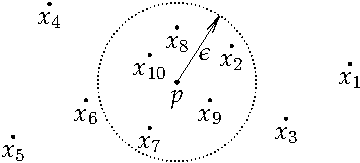
\includegraphics{figures/sequence-convergence-metric}
\caption{Barisan yang konvergen ke $p$. Sepuluh titik pertama
ditampilkan dan $M=7$ untuk $\epsilon$ ini.\label{fig:sequence-convergence-metric}}
\end{myfig}
\end{defn}

\begin{prop} \label{prop:mslimisunique}
Suatu barisan konvergen dalam ruang metrik memiliki limit tunggal.
\end{prop}

\begin{proof}
Andaikan barisan $\{ x_n \}$ memiliki limit $x$ dan $y$.
Ambil sebarang $\epsilon > 0$.
Dari definisi, carilah $n$ sedemikian sehingga
$d(x_n,x) < \nicefrac{\epsilon}{2}$ dan
$d(x_n,y) < \nicefrac{\epsilon}{2}$. Maka
\begin{equation*}
d(y,x)
\leq
d(y,x_n) + d(x_n,x)
<
\frac{\epsilon}{2} + \frac{\epsilon}{2} = \epsilon .
\end{equation*}
Jadi $x=y$, dan limit (jika ada) bersifat tunggal.
\end{proof}

Bukti proposisi-proposisi berikut diserahkan sebagai latihan.

\begin{prop} \label{prop:msconvbound}
Suatu barisan konvergen dalam ruang metrik bersifat terbatas.
\end{prop}

\begin{prop} \label{prop:msconvifa}
Suatu barisan $\{ x_n \}$ dalam ruang metrik $(X,d)$ konvergen ke $p \in X$
jika dan hanya
jika terdapat barisan bilangan real $\{ a_n \}$ sedemikian sehingga
\begin{equation*}
d(x_n,p) \leq a_n \quad \text{untuk semua } n \in \N,
\qquad \text{dan} \qquad
\lim_{n\to\infty} a_n = 0.
\end{equation*}
\end{prop}

\begin{prop} \label{prop:mssubseq}
Misalkan $\{ x_n \}$ suatu barisan dalam ruang metrik $(X,d)$.
\begin{enumerate}[(i)]
\item Jika $\{ x_n \}$ konvergen ke $p \in X$, maka setiap subbarisan $\{ x_{n_k} \}$
konvergen ke $p$.
\item Jika untuk suatu $K \in \N$, ekor-$K$ $\{ x_n \}_{n=K+1}^\infty$
konvergen ke $p \in X$, maka
 $\{ x_n \}$ konvergen ke $p$.
\end{enumerate}
\end{prop}

\begin{exbox}
\begin{exercise}
Buktikan \propref{prop:msconvbound}.
\end{exercise}

\begin{exercise}
Buktikan \propref{prop:msconvifa}.
\end{exercise}

\begin{exercise}
Buktikan \propref{prop:mssubseq}.
\end{exercise}
\end{exbox}

\begin{example}
Himpunan fungsi kontinu $C([a,b],\R)$, lihat \exampleref{example:msC01},
adalah ruang metrik. Kekonvergenan suatu barisan fungsi
dalam ruang metrik ini sama dengan kekonvergenan seragam. Lihat juga
\sectionref{sec:puconv} dalam lampiran berikutnya.
\end{example}

\begin{exbox}
\begin{exercise}
\begin{exparts}
\item
Tunjukkan bahwa $d(x,y) = \min \bigl\{ 1, \sabs{x-y} \bigr\}$ mendefinisikan suatu metrik pada $\R$.
\item
Tunjukkan bahwa suatu barisan konvergen dalam $(\R,d)$ jika dan hanya jika ia konvergen
dalam metrik standar.
\item
Carilah suatu barisan terbatas dalam $(\R,d)$ yang
tidak memuat subbarisan konvergen.
\end{exparts}
\end{exercise}

\begin{exercise}
Andaikan $\{x_n\}_{n=1}^\infty$ konvergen ke $x$. Andaikan $f \colon \N
\to \N$ fungsi satu-satu. Tunjukkan bahwa
$\{ x_{f(n)} \}_{n=1}^\infty$ konvergen ke $x$.
\end{exercise}

\begin{exercise}
Misalkan $(X,d)$ ruang metrik dengan $d$ metrik diskret. Andaikan
$\{ x_n \}$ suatu barisan konvergen dalam $X$. Tunjukkan bahwa terdapat
$K \in \N$ sedemikian sehingga untuk semua $n \geq K$, berlaku $x_n = x_K$.
\end{exercise}

\begin{exercise}
Suatu himpunan $S \subset X$ dikatakan \emph{padat} dalam $X$ jika
$X \subset \widebar{S}$ atau, dengan kata lain, jika untuk setiap $x \in X$,
terdapat suatu barisan $\{ x_n \}$ dalam $S$ yang konvergen ke $x$. Buktikan
bahwa $\R^n$ memuat suatu himpunan bagian padat yang terhitung.
\end{exercise}

\begin{exercise} \label{exercise:extendedrealsmetric}
Ambil $\R^* = \{ -\infty \} \cup \R \cup \{ \infty \}$ sebagai bilangan real diperluas.
Definisikan $d(x,y) = \babs{\frac{x}{1+\sabs{x}} - \frac{y}{1+\sabs{y}}}$
jika $x, y \in \R$,
definisikan $d(\infty,x) = \babs{1 - \frac{x}{1+\sabs{x}}}$,
$d(-\infty,x) = \babs{1 + \frac{x}{1+\sabs{x}}}$
untuk semua $x \in \R$, dan
ambil $d(\infty,-\infty) = 2$.
\begin{exparts}
\item
Tunjukkan bahwa $(\R^*,d)$ adalah ruang metrik.
\item
Andaikan $\{ x_n \}$ suatu barisan bilangan real sedemikian sehingga
untuk setiap $M \in \R$, terdapat $N$ sedemikian sehingga
$x_n \geq M$ untuk semua $n \geq N$. Tunjukkan bahwa $\lim\, x_n = \infty$ dalam
$(\R^*,d)$.
\item
Tunjukkan bahwa suatu barisan bilangan real konvergen ke bilangan real
dalam $(\R^*,d)$ jika dan
hanya jika ia konvergen dalam $\R$ dengan metrik standar.
\end{exparts}
\end{exercise}

\begin{exercise}
Misalkan $(X,d)$ ruang metrik dan $\{ x_n \}$ suatu barisan dalam $X$.
Buktikan bahwa $\{ x_n \}$ konvergen ke $p \in X$
jika dan hanya jika
setiap subbarisan dari $\{ x_n \}$ memiliki subbarisan yang
konvergen ke $p$.
\end{exercise}
\end{exbox}

\subsection{Kekonvergenan dalam ruang Euklides}

Dalam $\R^n$, suatu barisan konvergen jika dan hanya jika setiap
komponennya konvergen:

\begin{prop} \label{prop:msconveuc}
Misalkan $\{ x_j \}_{j=1}^\infty$ suatu barisan dalam $\R^n$,
dengan $x_j = \bigl(x_{j,1},x_{j,2},\ldots,x_{j,n}\bigr) \in \R^n$.
Maka $\{ x_j \}_{j=1}^\infty$ konvergen jika dan hanya jika
$\{ x_{j,k} \}_{j=1}^\infty$ konvergen untuk setiap $k=1,2,\ldots,n$; dalam hal ini
\begin{equation*}
\lim_{j\to\infty}
x_j =
\Bigl(
\lim_{j\to\infty} x_{j,1},
\lim_{j\to\infty} x_{j,2},
\ldots,
\lim_{j\to\infty} x_{j,n}
\Bigr) .
\end{equation*}
\end{prop}

\begin{proof}
Andaikan
barisan
$\{ x_j \}_{j=1}^\infty$ konvergen ke
$y = (y_1,y_2,\ldots,y_n) \in \R^n$.
Untuk $\epsilon > 0$, terdapat $M$ sedemikian sehingga untuk semua
$j \geq M$,
\begin{equation*}
d(y,x_j) < \epsilon.
\end{equation*}
Tetapkan suatu $k=1,2,\ldots,n$. Untuk $j \geq M$,
\begin{equation*}
\bigl\lvert y_k - x_{j,k} \bigr\rvert
=
\sqrt{{\bigl(y_k - x_{j,k} \bigr)}^2}
\leq
\sqrt{\sum_{\ell=1}^n {\bigl(y_\ell-x_{j,\ell}\bigr)}^2}
= d(y,x_j) < \epsilon .
\end{equation*}
Dengan demikian, barisan $\{ x_{j,k} \}_{j=1}^\infty$ konvergen ke $y_k$.

Untuk arah sebaliknya, andaikan
$\{ x_{j,k} \}_{j=1}^\infty$ konvergen ke $y_k$ untuk setiap $k=1,2,\ldots,n$.
Untuk $\epsilon > 0$, pilih $M$ sedemikian sehingga jika $j \geq M$, maka
$\bigl\lvert y_k-x_{j,k} \bigr\rvert < \nicefrac{\epsilon}{\sqrt{n}}$ untuk semua
$k=1,2,\ldots,n$. Maka
\begin{equation*}
d(y,x_j)
=
\sqrt{\sum_{k=1}^n {\bigl(y_k-x_{j,k}\bigr)}^2}
<
\sqrt{\sum_{k=1}^n {\left(\frac{\epsilon}{\sqrt{n}}\right)}^2}
=
\sqrt{\sum_{k=1}^n \frac{{\epsilon^2}}{n}}
= \epsilon .
\end{equation*}
Artinya, barisan $\{ x_j \}$ konvergen ke
$y = (y_1,y_2,\ldots,y_n) \in \R^n$.
\end{proof}

\begin{example}
Untuk $\C$, proposisi tersebut menyatakan bahwa
$\{ z_j \}_{j=1}^\infty = \{ x_j + iy_j \}_{j=1}^\infty$ konvergen
ke $z = x+iy$
jika dan hanya jika $\{ x_j \}$ konvergen ke $x$ dan
$\{ y_j \}$ konvergen ke $y$.
\end{example}

\begin{exbox}
\begin{exercise}
Tinjau $\R^n$, dan misalkan $d$ metrik Euklides standar.
Misalkan $d'(x,y) = \sum_{\ell=1}^n \sabs{x_\ell-y_\ell}$
dan $d''(x,y) = \max \bigl\{ \sabs{x_1-y_1},\sabs{x_2-y_2},\cdots,\sabs{x_n-y_n}
\bigr\}$.
\begin{exparts}
\item
Gunakan \exerciseref{exercise:mscross} untuk menunjukkan bahwa
$(\R^n,d')$ dan
$(\R^n,d'')$ adalah ruang metrik.
\item
Misalkan $\{ x_j \}_{j=1}^\infty$ suatu barisan dalam $\R^n$ dan $p \in \R^n$.
Buktikan bahwa pernyataan-pernyataan berikut ekuivalen:
\begin{exnumparts}
\item
$\{ x_j \}$ konvergen ke $p$ dalam $(\R^n,d)$.
\item
$\{ x_j \}$ konvergen ke $p$ dalam $(\R^n,d')$.
\item
$\{ x_j \}$ konvergen ke $p$ dalam $(\R^n,d'')$.
\end{exnumparts}
\end{exparts}
\end{exercise}
\end{exbox}

\subsection{Kekonvergenan dan topologi}

Topologi---himpunan semua himpunan terbuka suatu ruang---menyandikan barisan mana yang
konvergen.

\begin{prop} \label{prop:msconvtopo}
Misalkan $(X,d)$ ruang metrik dan $\{x_n\}$ suatu barisan dalam $X$. Maka
$\{ x_n \}$ konvergen ke $x \in X$ jika dan hanya jika untuk setiap lingkungan terbuka
$U$ dari $x$, terdapat $M \in \N$ sedemikian sehingga untuk semua $n \geq M$,
berlaku $x_n \in U$.
\end{prop}

\begin{proof}
Andaikan $\{ x_n \}$ konvergen ke $x$. Misalkan $U$ suatu lingkungan terbuka
dari $x$. Terdapat $\epsilon > 0$ sedemikian sehingga $B(x,\epsilon) \subset
U$. Karena barisan tersebut konvergen, carilah $M \in \N$ sedemikian sehingga untuk semua $n \geq
M$, berlaku $d(x,x_n) < \epsilon$, atau dengan kata lain $x_n \in B(x,\epsilon)
\subset U$.

Mari kita buktikan arah sebaliknya. Untuk $\epsilon > 0$, ambil $U =
B(x,\epsilon)$ sebagai lingkungan dari $x$. Maka terdapat $M \in \N$
sedemikian sehingga untuk $n \geq M$, berlaku $x_n \in U = B(x,\epsilon)$, atau dengan kata
lain, $d(x,x_n) < \epsilon$.
\end{proof}

Suatu himpunan tertutup memuat limit barisan-barisan konvergennya.

\begin{prop} \label{prop:msclosedlim}
Misalkan $(X,d)$ ruang metrik, $E \subset X$ suatu himpunan tertutup,
dan $\{ x_n \}$ suatu barisan dalam $E$ yang konvergen ke suatu $x \in X$.
Maka $x \in E$.
\end{prop}

\begin{proof}
Mari kita buktikan kontraposisinya.
Andaikan $\{ x_n \}$ suatu barisan dalam $X$ yang konvergen ke $x \in E^c$.
Karena $E^c$ terbuka, \propref{prop:msconvtopo} menyatakan bahwa terdapat
$M$ sedemikian sehingga untuk semua $n \geq M$,
$x_n \in E^c$. Jadi $\{ x_n \}$ bukan barisan dalam $E$.
\end{proof}

Untuk mengambil penutupan suatu himpunan $A$, kita mengambil $A$, lalu memasukkan
titik-titik yang merupakan limit barisan dalam $A$.

\begin{prop} \label{prop:msclosureapprseq}
Misalkan $(X,d)$ ruang metrik dan $A \subset X$.
Maka $x \in \widebar{A}$ jika dan hanya jika terdapat suatu barisan $\{ x_n \}$ dari
elemen-elemen dalam $A$ sedemikian sehingga $\lim\, x_n = x$.
\end{prop}

\begin{proof}
Misalkan $x \in \widebar{A}$. Untuk setiap $n \in \N$,
menurut
\propref{prop:msclosureappr}, terdapat
suatu titik $x_n \in B(x,\nicefrac{1}{n}) \cap A$.
Karena $d(x,x_n) < \nicefrac{1}{n}$, kita peroleh $\lim\, x_n = x$.

Untuk arah sebaliknya, lihat \exerciseref{exercise:reverseclosedseq}.
\end{proof}

\begin{exbox}
\begin{exercise}%[\neededexmark]
\label{exercise:reverseclosedseq}
Selesaikan bukti
\propref{prop:msclosureapprseq}:
Misalkan $(X,d)$ ruang metrik dan
$A \subset X$. Misalkan $x \in X$
sedemikian sehingga terdapat suatu barisan $\{ x_n \}$ dalam $A$ yang konvergen ke $x$.
Buktikan bahwa $x \in \widebar{A}$.
\end{exercise}

\begin{exercise}
Andaikan $\{ U_n \}_{n=1}^\infty$ suatu barisan menurun ($U_{n+1} \subset U_n$ untuk
semua $n$) dari himpunan-himpunan terbuka dalam ruang metrik $(X,d)$ sedemikian sehingga
$\bigcap_{n=1}^\infty U_n = \{ p \}$ untuk suatu $p \in X$. Andaikan
$\{ x_n \}$ suatu barisan titik dalam $X$ sedemikian sehingga $x_n \in U_n$. Apakah
$\{ x_n \}$ harus konvergen ke $p$? Buktikan atau konstruksikan contoh penyangkal.
\end{exercise}

\begin{exercise}
Misalkan $E \subset X$ tertutup dan
misalkan $\{ x_n \}$ suatu barisan dalam $X$ yang konvergen ke $p \in X$. Andaikan
$x_n \in E$ untuk tak hingga banyak $n \in \N$. Tunjukkan bahwa $p \in E$.
\end{exercise}

\begin{exercise}
Andaikan $\{ V_n \}_{n=1}^\infty$ suatu barisan himpunan terbuka
dalam $(X,d)$
sedemikian sehingga $V_{n+1} \supset V_n$ untuk semua $n$. Misalkan $\{ x_n \}$ suatu barisan
sedemikian sehingga $x_n \in V_{n+1} \setminus V_n$ dan andaikan
$\{ x_n \}$ konvergen ke $p \in X$. Tunjukkan bahwa $p \in \partial V$
dengan $V = \bigcup_{n=1}^\infty V_n$.
\end{exercise}
\end{exbox}

%%%%%%%%%%%%%%%%%%%%%%%%%%%%%%%%%%%%%%%%%%%%%%%%%%%%%%%%%%%%%%%%%%%%%%%%%%%%%%

\section{Kelengkapan dan kekompakan}
\label{sec:metcompact}

\subsection{Barisan Cauchy dan kelengkapan}

\begin{defn}
Misalkan $(X,d)$ ruang metrik.
Suatu barisan $\{ x_n \}$ dalam $X$ adalah \emph{\myindex{barisan Cauchy}} jika
untuk setiap $\epsilon > 0$, terdapat $M \in \N$ sedemikian sehingga
untuk semua $n \geq M$ dan semua $k \geq M$, berlaku
\begin{equation*}
d(x_n, x_k) < \epsilon .
\end{equation*}
\end{defn}

\begin{prop}
Suatu barisan konvergen dalam ruang metrik adalah barisan Cauchy.
\end{prop}

\begin{proof}
Andaikan $\{ x_n \}$ konvergen ke $x$.
Untuk $\epsilon > 0$, terdapat $M$ sedemikian sehingga
$d(x,x_n) < \nicefrac{\epsilon}{2}$ untuk semua $n \geq M$.
Oleh karena itu,
$d(x_n,x_k) \leq d(x_n,x) + d(x,x_k) < \nicefrac{\epsilon}{2} +
\nicefrac{\epsilon}{2} = \epsilon$
untuk semua $n,k \geq M$.
\end{proof}

\begin{defn}
Misalkan $(X,d)$ ruang metrik. Kita mengatakan bahwa $X$
\emph{\myindex{lengkap}} atau \emph{\myindex{lengkap-Cauchy}}
jika setiap barisan Cauchy $\{ x_n \}$ dalam $X$
konvergen ke suatu $x \in X$.
\end{defn}

\begin{prop}
Ruang $\R^n$ dengan metrik standar merupakan ruang metrik lengkap.
\end{prop}

Kita mengandaikan bahwa pembaca telah melihat bukti kelengkapan dalam $\R = \R^1$,
dan kita mereduksi kelengkapan dalam $\R^n$ ke kasus satu dimensi.

\begin{proof}
Misalkan $\{ x_j \}_{j=1}^\infty$ suatu barisan Cauchy
dalam $\R^n$, dengan $x_j = \bigl(x_{j,1},x_{j,2},\ldots,x_{j,n}\bigr) \in \R^n$.
Untuk $\epsilon > 0$, terdapat $M$ sedemikian sehingga
$d(x_i,x_j) < \epsilon$
untuk semua
$i,j \geq M$.

Tetapkan suatu $k=1,2,\ldots,n$. Untuk $i,j \geq M$,
\begin{equation*}
\bigl\lvert x_{i,k} - x_{j,k} \bigr\rvert
=
\sqrt{{\bigl(x_{i,k} - x_{j,k}\bigr)}^2}
\leq
\sqrt{\sum_{\ell=1}^n {\bigl(x_{i,\ell}-x_{j,\ell}\bigr)}^2}
= d(x_i,x_j) < \epsilon .
\end{equation*}
Dengan demikian, barisan $\{ x_{j,k} \}_{j=1}^\infty$ adalah barisan Cauchy. Karena $\R$
lengkap, barisan tersebut konvergen; terdapat $y_k \in \R$ sedemikian sehingga
$y_k = \lim_{j\to\infty} x_{j,k}$.
Tuliskan $y = (y_1,y_2,\ldots,y_n) \in \R^n$.
Menurut \propref{prop:msconveuc}, $\{ x_j \}$ konvergen
ke $y \in \R^n$, sehingga $\R^n$ lengkap.
\end{proof}

Suatu himpunan bagian dari $\R^n$ dengan metrik subruang tidak harus
lengkap. Sebagai contoh, $(0,1]$ dengan metrik subruang tidak
lengkap karena $\{ \nicefrac{1}{n} \}$ adalah barisan Cauchy dalam $(0,1]$
yang tidak memiliki limit dalam $(0,1]$.
Namun,
begitu kita memiliki satu ruang metrik lengkap, setiap subruang tertutup juga
merupakan ruang metrik lengkap. Lagi pula, salah satu cara
untuk memandang suatu himpunan tertutup adalah bahwa ia memuat semua titik
yang dapat dicapai dari himpunan tersebut melalui suatu barisan.
Buktinya sekali lagi menjadi latihan.

\begin{prop} \label{prop:closedcomplete}
Andaikan $(X,d)$ ruang metrik lengkap dan $E \subset X$
tertutup. Maka $E$ merupakan ruang metrik lengkap dengan topologi subruang.
\end{prop}

\begin{exbox}
\begin{exercise}%[\neededexmark]
Buktikan \propref{prop:closedcomplete}.
\end{exercise}
\end{exbox}

\begin{example}
Contoh lain yang sangat berguna dari ruang metrik lengkap adalah ruang
fungsi-fungsi kontinu pada interval tertutup dengan norma seragam, $C([a,b],\R)$.
Lihat \corref{cor:CSRcomplete} dalam lampiran berikutnya.
\end{example}

\subsection{Kekompakan}

\begin{defn}
Misalkan $(X,d)$ ruang metrik dan $K \subset X$.
Himpunan $K$ dikatakan \emph{\myindex{kompak}}
jika untuk setiap koleksi
himpunan terbuka $\{ U_{\lambda} \}_{\lambda \in I}$ sedemikian sehingga
\begin{equation*}
K \subset \bigcup_{\lambda \in I} U_\lambda ,
\end{equation*}
terdapat himpunan bagian berhingga
$\{ \lambda_1, \lambda_2,\ldots,\lambda_k \} \subset I$
sedemikian sehingga
\begin{equation*}
K \subset U_{\lambda_1} \cup U_{\lambda_2} \cup \cdots \cup U_{\lambda_k} .
\end{equation*}
\end{defn}

Suatu koleksi himpunan terbuka $\{ U_{\lambda} \}_{\lambda \in I}$ seperti di atas
disebut \emph{\myindex{penutup terbuka}} dari $K$. Salah satu cara untuk menyatakan bahwa
$K$ kompak adalah dengan mengatakan bahwa \emph{setiap penutup terbuka dari $K$ memiliki
\myindex{subpenutup} berhingga}.

\begin{example}
Misalkan $\R$ ruang metrik dengan metrik standar.

Himpunan $\R$ tidak kompak. Bukti: Ambil himpunan-himpunan $U_n = (-n,n)$.
Ini merupakan penutup terbuka, tetapi gabungan suatu subhimpunan berhingga dari himpunan-himpunan tersebut
hanyalah $(-n,n)$ untuk suatu $n$.

Himpunan $(0,1) \subset \R$ juga tidak kompak. Bukti: Ambil
himpunan-himpunan $U_{n} = (\nicefrac{1}{n},1-\nicefrac{1}{n})$ untuk $n=3,4,5,\ldots$.
Seperti di atas, $(0,1) = \bigcup_{n=3}^\infty U_n$, tetapi gabungan sejumlah berhingga darinya
kembali hanya $U_n$ dan bukan seluruh $(0,1)$.

Himpunan $\{ 0 \} \subset \R$ kompak. Bukti: Untuk sebarang penutup terbuka $\{
U_{\lambda} \}_{\lambda \in I}$, harus terdapat $\lambda_0$ sedemikian sehingga $0
\in U_{\lambda_0}$ karena koleksi tersebut merupakan penutup, sehingga $U_{\lambda_0}$ memberikan
subpenutup berhingga.

Di bawah ini kita akan membuktikan bahwa $[0,1]$, dan bahkan setiap interval tertutup dan terbatas
$[a,b]$, bersifat kompak.
\end{example}

\begin{exbox}
\begin{exercise}
Misalkan $(X,d)$ ruang metrik dan $A$ suatu himpunan bagian berhingga dari $X$.
Tunjukkan bahwa $A$ kompak.
\end{exercise}

\begin{exercise}
Misalkan $A = \{ \nicefrac{1}{n} : n \in \N \} \subset \R$.
\begin{exparts}
\item
Tunjukkan secara langsung dengan menggunakan definisi bahwa $A$
tidak kompak.
\item
Tunjukkan secara langsung dengan menggunakan definisi bahwa $A \cup \{ 0 \}$
kompak.
\end{exparts}
\end{exercise}

\begin{exercise}
\begin{exparts}
\item
Tunjukkan bahwa gabungan sejumlah berhingga himpunan kompak adalah himpunan kompak.
\item
Carilah contoh ketika gabungan tak hingga banyak himpunan kompak tidak
kompak.
\end{exparts}
\end{exercise}
\end{exbox}

\begin{prop}
Misalkan $(X,d)$ ruang metrik. Suatu himpunan kompak $K \subset X$ tertutup dan
terbatas.
\end{prop}

\begin{proof}
Misalkan $K$ suatu himpunan kompak.
Tetapkan $p \in X$. Kita memiliki penutup terbuka
\begin{equation*}
K \subset \bigcup_{n=1}^\infty B(p,n) = X .
\end{equation*}
Jika $K$ kompak, maka terdapat suatu himpunan indeks
$n_1 < n_2 < \ldots < n_k$ sedemikian sehingga
\begin{equation*}
K \subset
B(p,n_1)
\cup
B(p,n_2)
\cup \cdots \cup
B(p,n_k)
= B(p,n_k) .
\end{equation*}
Jadi $K$ terbatas.
Lihat bagian kiri \figureref{fig:compactbndclosed}.

Selanjutnya, kita tunjukkan bahwa suatu himpunan yang tidak tertutup tidak kompak. Andaikan
$\widebar{K} \neq K$, yaitu terdapat suatu titik $x \in \widebar{K}
\setminus K$.
Kita memiliki penutup terbuka
\begin{equation*}
K \subset \bigcup_{n=1}^\infty {C(x,\nicefrac{1}{n})}^c .
\end{equation*}
Jika kita mengambil sebarang
koleksi indeks berhingga $n_1 < n_2 < \ldots < n_k$, maka
\begin{equation*}
{C(x,\nicefrac{1}{n_1})}^c
\cup
{C(x,\nicefrac{1}{n_2})}^c
\cup \cdots \cup
{C(x,\nicefrac{1}{n_k})}^c
=
{C(x,\nicefrac{1}{n_k})}^c
\end{equation*}
Karena $x$ berada dalam penutupan $K$,
kita memiliki
$C(x,\nicefrac{1}{n_k}) \cap K \neq \emptyset$. Jadi tidak ada
subpenutup berhingga dan $K$ tidak kompak.
Lihat bagian kanan \figureref{fig:compactbndclosed}.
\end{proof}

\begin{myfig}
\subimport*{figures/}{compactbnd.pdf_t}
\qquad \qquad
\subimport*{figures/}{compactclosed.pdf_t}
\caption{Pembuktian bahwa himpunan kompak terbatas (kiri) dan tertutup (kanan).\label{fig:compactbndclosed}}
\end{myfig}

Di bawah ini kita membuktikan bahwa
dalam ruang Euklides berdimensi hingga,
setiap himpunan tertutup dan terbatas bersifat kompak.
Jadi, himpunan tertutup dan terbatas
dari $\R^n$ merupakan contoh himpunan kompak.
Tidak benar bahwa dalam setiap ruang metrik, tertutup dan terbatas ekuivalen
dengan kompak. Contoh sederhana adalah ruang metrik tak lengkap seperti
$(0,1)$ dengan metrik subruang dari $\R$.
Terdapat banyak ruang metrik lengkap yang sangat berguna
di mana tertutup dan terbatas tidak
cukup untuk menghasilkan kekompakan: $C([a,b],\R)$ adalah ruang metrik lengkap,
tetapi bola satuan tertutup $C(0,1)$ tidak kompak, lihat
\exerciseref{exercise:msclbounnotcompt}. Namun, lihat juga
\exerciseref{exercise:mstotbound}. Karena persoalan ini merupakan kekeliruan yang begitu umum, izinkan saya
mengulanginya dengan huruf miring: \emph{Tertutup dan terbatas tidak sama dengan kompak.}

Sifat yang berguna dari himpunan kompak dalam ruang metrik adalah bahwa setiap
barisan dalam himpunan tersebut memiliki subbarisan konvergen yang konvergen
ke suatu titik dalam himpunan tersebut.
Himpunan demikian disebut
\emph{\myindex{kompak sekuensial}}.
Mari kita buktikan bahwa dalam
konteks ruang metrik, suatu himpunan kompak jika dan hanya jika ia kompak
sekuensial.
Pertama-tama kita buktikan sebuah lema.

\begin{lemma}[Lema penutup Lebesgue%
\footnote{Bilangan $\delta$ kadang-kadang disebut
\myindex{bilangan Lebesgue} dari penutup tersebut.}]\label{ms:lebesgue}
\index{lema penutup Lebesgue}
Misalkan $(X,d)$ ruang metrik dan $K \subset X$. Andaikan
setiap barisan dalam $K$ memiliki subbarisan yang konvergen dalam $K$. Untuk
suatu penutup terbuka $\{ U_\lambda \}_{\lambda \in I}$ dari $K$, terdapat
$\delta > 0$ sedemikian sehingga untuk setiap $x \in K$, terdapat $\lambda \in I$
dengan $B(x,\delta) \subset U_\lambda$.
\end{lemma}

\begin{proof}
Kita membuktikan lema tersebut melalui kontraposisi.
Jika kesimpulannya tidak benar, maka
terdapat
suatu penutup terbuka $\{ U_\lambda \}_{\lambda \in I}$ dari $K$ dengan
sifat berikut.
Untuk setiap $n \in \N$, terdapat $x_n \in K$ sedemikian sehingga
$B(x_n,\nicefrac{1}{n})$ bukan himpunan bagian dari satu pun $U_\lambda$.
Ambil sebarang $x \in K$. Terdapat
$\lambda \in I$ sedemikian sehingga $x \in U_\lambda$. Karena $U_\lambda$ terbuka,
terdapat $\epsilon > 0$
sedemikian sehingga $B(x,\epsilon) \subset U_\lambda$. Ambil $M$ sedemikian sehingga
$\nicefrac{1}{M} < \nicefrac{\epsilon}{2}$. Jika $y \in
B(x,\nicefrac{\epsilon}{2})$ dan $n \geq M$, maka
\begin{equation*}
B(y,\nicefrac{1}{n}) \subset
B(y,\nicefrac{1}{M}) \subset
B(y,\nicefrac{\epsilon}{2}) \subset B(x,\epsilon)
\subset U_\lambda ,
\end{equation*}
di mana
$B(y,\nicefrac{\epsilon}{2}) \subset B(x,\epsilon)$
mengikuti ketaksamaan segitiga.
Lihat \figureref{fig:lebesguedelta}.
Dengan demikian, $y \neq x_n$.
Dengan kata lain, untuk semua $n \geq M$, $x_n \notin B(x,\nicefrac{\epsilon}{2})$.
Barisan tersebut tidak dapat memiliki subbarisan yang konvergen ke $x$. Karena $x \in K$ dipilih
secara sebarang, kita selesai.
\end{proof}

\begin{myfig}
\subimport*{figures/}{lebesguedelta.pdf_t}
\caption{Bukti lema penutup Lebesgue.
Perhatikan bahwa $B(y,\nicefrac{\epsilon}{2}) \subset
B(x,\epsilon)$ menurut ketaksamaan segitiga.\label{fig:lebesguedelta}}
\end{myfig}

Penting untuk mengenali apa yang dinyatakan oleh lema tersebut. Lema itu menyatakan bahwa
jika $K$ kompak sekuensial, maka untuk setiap penutup yang diberikan,
terdapat satu $\delta > 0$. Nilai $\delta$ bergantung pada penutup tersebut,
tetapi tentu saja tidak bergantung pada $x$.

Sebagai contoh, misalkan $K = [-10,10]$ dan untuk $n \in \Z$, biarkan $U_n =
(n,n+2)$ mendefinisikan suatu penutup terbuka.
Ambil $x \in K$. Terdapat $n \in \Z$
sedemikian sehingga $n \leq x < n+1$.
Jika $n \leq x < n+\nicefrac{1}{2}$, maka
$B\bigl(x,\nicefrac{1}{2}\bigr) \subset U_{n-1}$.
Jika $n+ \nicefrac{1}{2} \leq x < n+1$, maka
$B\bigl(x,\nicefrac{1}{2}\bigr) \subset U_{n}$. Jadi $\delta =
\nicefrac{1}{2}$. Jika sebagai gantinya kita mengambil penutup terbuka oleh $U'_n =
\bigl(\frac{n}{2},\frac{n+2}{2} \bigr)$, nilai $\delta$ terbaik adalah $\nicefrac{1}{4}$.

\begin{thm} \label{thm:mscompactisseqcpt}
Misalkan $(X,d)$ ruang metrik. Maka $K \subset X$ kompak jika
dan hanya jika setiap barisan dalam $K$ memiliki subbarisan yang konvergen ke
suatu titik dalam $K$.
\end{thm}

\begin{proof}
Klaim: \emph{Misalkan $K \subset X$ suatu himpunan bagian dari $X$ dan
$\{ x_n \}$ suatu barisan dalam $K$. Andaikan bahwa untuk setiap $x \in K$,
terdapat bola $B(x,\alpha_x)$ untuk suatu $\alpha_x > 0$ sedemikian sehingga
$x_n \in B(x,\alpha_x)$ hanya untuk sejumlah berhingga $n \in \N$.
Maka $K$ tidak kompak.}

Bukti klaim:
Perhatikan
\begin{equation*}
K \subset \bigcup_{x \in K} B(x,\alpha_x) .
\end{equation*}
Setiap koleksi berhingga bola-bola ini hanya memuat sejumlah berhingga
elemen dari $\{ x_n \}$,
sehingga harus ada suatu $x_n \in K$
yang tidak berada dalam gabungannya. Oleh karena itu, $K$ tidak kompak dan klaim
terbukti.

Andaikan $K$ kompak dan $\{ x_n \}$ suatu barisan dalam $K$.
Maka terdapat $x \in K$ sedemikian sehingga
untuk setiap $\delta > 0$,
$B(x,\delta)$ memuat $x_k$ untuk tak hingga banyak $k \in \N$.
Bola $B(x,1)$ memuat suatu $x_k$, jadi ambil $n_1 = k$.
Andaikan $n_{j-1}$ telah didefinisikan.
Harus terdapat $\ell > n_{j-1}$
sedemikian sehingga $x_\ell \in B(x,\nicefrac{1}{j})$. Definisikan
$n_j = \ell$.
Sekarang kita memiliki suatu subbarisan $\{ x_{n_j} \}_{j=1}^\infty$.
Karena
$d(x,x_{n_j}) < \nicefrac{1}{j}$, \propref{prop:msconvifa} menyatakan bahwa
$\lim\, x_{n_j} = x$.

Untuk arah sebaliknya, andaikan setiap barisan dalam $K$
memiliki suatu
subbarisan yang konvergen dalam $K$.
Ambil
suatu penutup terbuka $\{ U_\lambda \}_{\lambda \in I}$ dari $K$.
Dengan menggunakan lema penutup Lebesgue di atas, carilah $\delta > 0$
sedemikian sehingga untuk setiap $x \in K$, terdapat $\lambda \in I$ dengan
$B(x,\delta) \subset U_\lambda$.

Pilih $x_1 \in K$ dan carilah $\lambda_1 \in I$ sedemikian sehingga $B(x_1,\delta) \subset
U_{\lambda_1}$.
Jika $K \subset U_{\lambda_1}$, kita berhenti karena telah menemukan
subpenutup berhingga.
Jika tidak, harus ada
suatu titik $x_2 \in K \setminus U_{\lambda_1}$.
Perhatikan bahwa $d(x_2,x_1) \geq \delta$.
Harus terdapat suatu $\lambda_2 \in I$ sedemikian sehingga
$B(x_2,\delta) \subset U_{\lambda_2}$.
Kita bekerja secara induktif. Andaikan $\lambda_{n-1}$ telah didefinisikan.
Entah
$U_{\lambda_1} \cup
U_{\lambda_2} \cup \cdots \cup
U_{\lambda_{n-1}}$ merupakan penutup berhingga dari $K$, dalam hal ini kita
berhenti, atau
harus ada
suatu titik $x_n \in K \setminus \bigl( U_{\lambda_1} \cup
U_{\lambda_2} \cup \cdots \cup
U_{\lambda_{n-1}}\bigr)$.
Perhatikan bahwa $d(x_n,x_j) \geq \delta$ untuk semua $j = 1,2,\ldots,n-1$.
Selanjutnya, harus ada suatu $\lambda_n \in I$
sedemikian sehingga $B(x_n,\delta) \subset U_{\lambda_n}$.
Lihat \figureref{fig:seqcompactiscompact}.

\begin{myfig}
\subimport*{figures/}{seqcompactiscompact.pdf_t}
\caption{Menutupi $K$ dengan $U_{\lambda}$. Titik-titik
$x_1,x_2,x_3,x_4$,
ketiga himpunan
$U_{\lambda_1}$,
$U_{\lambda_2}$,
$U_{\lambda_2}$,
dan
tiga bola pertama
berjari-jari $\delta$ digambar.\label{fig:seqcompactiscompact}}
\end{myfig}

Entah pada suatu tahap kita memperoleh subpenutup berhingga dari $K$,
atau kita memperoleh suatu
barisan tak hingga
$\{ x_n \}$ seperti di atas.
Untuk memperoleh kontradiksi, andaikan
tidak ada subpenutup berhingga dan kita memiliki barisan $\{ x_n \}$ tersebut.
Untuk semua $n$ dan $k$, $n \neq k$,
berlaku $d(x_n,x_k) \geq \delta$,
sehingga tidak ada subbarisan dari $\{ x_n \}$ yang dapat menjadi
barisan Cauchy. Dengan demikian, tidak ada subbarisan dari $\{ x_n \}$ yang dapat konvergen,
yang merupakan kontradiksi.
\end{proof}

\begin{example}
Teorema Bolzano--Weierstrass untuk barisan bilangan real
menyatakan bahwa suatu barisan terbatas dalam $\R$ memiliki subbarisan
konvergen. Oleh karena itu, setiap barisan dalam interval tertutup $[a,b] \subset \R$ memiliki
subbarisan konvergen. Limitnya juga harus berada dalam $[a,b]$ karena limit
mempertahankan ketaksamaan tak ketat. Dengan demikian, interval tertutup dan terbatas $[a,b]
\subset \R$ bersifat kompak.
\end{example}

\begin{prop}
Misalkan $(X,d)$ ruang metrik dan misalkan $K \subset X$ kompak. Jika
$E \subset K$ suatu himpunan tertutup, maka $E$ kompak.
\end{prop}

\begin{proof}
Karena $K$ tertutup, $E$ tertutup dalam $K$ jika
dan hanya jika ia tertutup dalam $X$.
Lihat \propref{prop:topology:subspacesame}.
Misalkan $\{ x_n \}$ suatu barisan dalam $E$. Barisan ini juga merupakan barisan dalam $K$.
Oleh karena itu, ia memiliki subbarisan konvergen $\{ x_{n_j} \}$ yang konvergen ke
suatu $x \in K$. Karena $E$ tertutup, limit suatu barisan dalam $E$ juga berada dalam $E$,
sehingga $x \in E$. Jadi $E$ harus kompak.
\end{proof}

\begin{thm}[Heine--Borel] \index{teorema Heine--Borel}
\label{thm:msbw}
Suatu himpunan bagian tertutup dan terbatas $K \subset \R^n$ bersifat kompak.
\end{thm}

Jadi, himpunan bagian dari $\R^n$ kompak jika dan hanya jika tertutup dan terbatas,
suatu syarat yang jauh lebih mudah diperiksa.
Mari kita tegaskan kembali bahwa teorema Heine--Borel hanya berlaku untuk $\R^n$ dan tidak
untuk ruang metrik secara umum. Secara umum, kompak mengakibatkan tertutup dan
terbatas, tetapi tidak sebaliknya.

\begin{proof}
Untuk $\R = \R^1$, jika $K \subset \R$ tertutup dan terbatas, maka
setiap barisan $\{ x_k \}$ dalam $K$ terbatas, sehingga ia memiliki subbarisan konvergen
menurut
teorema Bolzano--Weierstrass.
Karena $K$ tertutup, limit subbarisan tersebut harus merupakan elemen
$K$. Jadi $K$ kompak.

Mari kita jalankan pembuktiannya untuk $n=2$ dan serahkan $n$ sebarang sebagai latihan.
Karena $K \subset \R^2$ terbatas, terdapat suatu himpunan
$B=[a,b]\times[c,d] \subset \R^2$ sedemikian sehingga $K \subset B$. Kita akan menunjukkan
bahwa $B$ kompak. Maka $K$, sebagai himpunan bagian tertutup dari $B$ yang kompak, juga
kompak.

Misalkan $\bigl\{ (x_k,y_k) \bigr\}_{k=1}^\infty$ suatu barisan dalam $B$. Artinya,
$a \leq x_k \leq b$ dan
$c \leq y_k \leq d$ untuk semua $k$. Suatu barisan bilangan real terbatas
memiliki subbarisan
konvergen, sehingga terdapat subbarisan $\{ x_{k_j} \}_{j=1}^\infty$
yang konvergen. Subbarisan
$\{ y_{k_j} \}_{j=1}^\infty$ juga merupakan barisan terbatas, sehingga terdapat
suatu subbarisan
$\{ y_{k_{j_\ell}} \}_{\ell=1}^\infty$ yang konvergen. Subbarisan dari suatu barisan
konvergen tetap konvergen, sehingga
$\{ x_{k_{j_\ell}} \}_{\ell=1}^\infty$ konvergen.
Ambil
\begin{equation*}
x = \lim_{\ell\to\infty} x_{k_{j_\ell}}
\qquad \text{dan} \qquad
y = \lim_{\ell\to\infty} y_{k_{j_\ell}} .
\end{equation*}
Menurut \propref{prop:msconveuc},
$\bigl\{ (x_{k_{j_\ell}},y_{k_{j_\ell}}) \bigr\}_{\ell=1}^\infty$ konvergen ke $(x,y)$.
Karena $a \leq x_k \leq b$ dan
$c \leq y_k \leq d$ untuk semua $k$, kita tahu bahwa $(x,y) \in B$.
\end{proof}

\begin{exbox}
\begin{exercise}
Buktikan \thmref{thm:msbw} untuk dimensi sebarang.
Petunjuk: Kuncinya adalah menggunakan notasi yang tepat.
\end{exercise}
\end{exbox}

\begin{prop}
Andaikan $(X,d)$ ruang metrik
dan $E_1$, $E_2$, \ldots, merupakan
himpunan bagian kompak tak kosong dari $X$ sedemikian sehingga
$E_1 \supset E_2 \supset E_3 \supset \cdots$. Maka
\begin{equation*}
\bigcap_{k=1}^\infty E_k \neq \emptyset .
\end{equation*}
\end{prop}

\begin{proof}
Andaikan $E_1,E_2,\ldots$ seperti dalam pernyataan, kecuali kita tidak
mengandaikan bahwa semuanya tidak kosong.
Himpunan kompak bersifat tertutup, sehingga komplemennya terbuka. Tinjau
$U_k = X \setminus E_k$. Andaikan irisannya kosong.
Maka $\{ U_k \}$ merupakan penutup terbuka dari $E_1$, yang kompak,
sehingga terdapat subpenutup berhingga.
Karena himpunan-himpunan tersebut tersarang,
$U_\ell \subset U_{\ell+1}$ untuk semua $\ell$,
kita memiliki $E_1 \subset U_k$ untuk suatu $k$. Dengan demikian, $E_k$ kosong.
\end{proof}

\begin{example}
Misalkan $(X,d)$ ruang metrik dengan metrik diskret, yaitu $d(x,y) = 1$
jika $x \neq y$. Andaikan
$X$ suatu himpunan tak hingga. Maka:
\begin{enumerate}[(i)]
\item $(X,d)$ adalah ruang metrik lengkap.
\item Setiap himpunan bagian $K \subset X$ tertutup dan terbatas.
\item Suatu himpunan bagian $K \subset X$ kompak jika dan hanya jika ia merupakan himpunan berhingga.
\item Kesimpulan lema penutup Lebesgue selalu dipenuhi
dengan sebarang $\delta \in (0,1)$, bahkan untuk $K \subset X$ yang tidak kompak.
\end{enumerate}
Bukti-bukti
pernyataan tersebut jelas atau diserahkan kepada latihan-latihan
di bawah ini.
\end{example}

\begin{remark}
Suatu hal yang halus mengenai barisan Cauchy, kelengkapan, kekompakan,
dan kekonvergenan adalah bahwa kekompakan dan kekonvergenan hanya bergantung pada
topologi, yaitu pada himpunan mana yang merupakan himpunan terbuka. Di sisi lain,
barisan Cauchy dan kelengkapan bergantung pada metrik yang sebenarnya.
\end{remark}

\begin{exbox}
\begin{exercise}
Misalkan $(X,d)$ ruang metrik dengan metrik diskret.
\begin{exparts}
\item
Buktikan bahwa $X$ lengkap.
\item
Buktikan bahwa $X$ kompak jika dan hanya jika $X$ suatu himpunan berhingga.
\end{exparts}
\end{exercise}

\begin{exercise}
Tunjukkan bahwa suatu himpunan kompak $K$ (dalam sebarang ruang metrik)
sendiri merupakan ruang metrik lengkap (dengan menggunakan metrik subruang).
\end{exercise}

\begin{exercise}
Tunjukkan bahwa terdapat suatu metrik pada $\R$ yang membuat $\R$ menjadi himpunan kompak.
\end{exercise}

\begin{exercise} \label{exercise:msclbounnotcompt}
Misalkan $C([0,1],\R)$ ruang metrik dari \exampleref{example:msC01}. Misalkan $0$
menyatakan fungsi nol. Tunjukkan bahwa bola tertutup
$C(0,1)$ tidak kompak (meskipun tertutup dan terbatas).
Petunjuk: Konstruksikan fungsi-fungsi kontinu $f_n \colon [0,1] \to \R$ sedemikian sehingga
$d(f_n,0) = 1$ dan $d(f_n,f_k) = 1$ untuk semua $n \neq k$.
\end{exercise}

\begin{exercise}
Misalkan $C([0,1],\R)$ adalah ruang metrik pada \exampleref{example:msC01}.
Misalkan $K$ adalah himpunan semua $f \in C([0,1],\R)$ sedemikian sehingga
$f$ sama dengan suatu polinom kuadratik, yaitu, $f(x) = a+bx+cx^2$, dan sedemikian sehingga
$\abs{f(x)} \leq 1$ untuk semua $x \in [0,1]$,
yakni $f \in C(0,1)$.  Tunjukkan bahwa $K$ kompak.
\end{exercise}

\begin{exercise} \label{exercise:mstotbound}
Misalkan $(X,d)$ adalah ruang metrik lengkap.
Tunjukkan bahwa $K \subset X$ kompak jika dan hanya jika $K$ tertutup
dan sedemikian sehingga untuk setiap $\epsilon > 0$
terdapat himpunan hingga titik-titik $x_1,x_2,\ldots,x_n$ dengan
$K \subset \bigcup_{j=1}^n B(x_j,\epsilon)$.
Catatan: Himpunan $K$ demikian disebut \emph{\myindex{terbatas total}},
jadi dalam ruang metrik lengkap, suatu himpunan kompak jika dan hanya
jika himpunan itu tertutup dan terbatas total.
\end{exercise}

\begin{exercise}
Ambil $\N \subset \R$ dengan metrik standar.  Carilah suatu selimut terbuka bagi $\N$
sedemikian sehingga kesimpulan lemma selimut Lebesgue tidak berlaku.
\end{exercise}

\begin{exercise}
Buktikan \myindex{teorema Bolzano--Weierstrass} yang umum:
Setiap barisan terbatas $\{ x_k
\}$ dalam $\R^n$ mempunyai suatu subbarisan konvergen.
\end{exercise}

\begin{exercise}
Misalkan $X$ adalah ruang metrik dan
$C$ adalah himpunan semua subhimpunan kompak tak kosong dari $X$.
Dengan menggunakan metrik Hausdorff dari \exerciseref{exercise:mshausdorffpseudo},
tunjukkan bahwa $(C,d_H)$ adalah ruang metrik.  Artinya, tunjukkan bahwa
jika $L$ dan $K$ adalah subhimpunan kompak tak kosong, maka $d_H(L,K) = 0$
jika dan hanya jika $L=K$.
\end{exercise}

\begin{exercise}
Misalkan $(X,d)$ adalah ruang metrik tak lengkap.  Tunjukkan bahwa terdapat suatu
himpunan tertutup dan terbatas $E \subset X$ yang tidak kompak.
\end{exercise}

\begin{exercise}
Misalkan $(X,d)$ adalah ruang metrik dan $K \subset X$.
Buktikan bahwa $K$ kompak sebagai subhimpunan dari $(X,d)$ jika dan hanya jika $K$
kompak sebagai subhimpunan dari dirinya sendiri dengan metrik subruang.
\end{exercise}

\begin{exercise}
Misalkan $(X,d)$ adalah ruang metrik lengkap.
Kita mengatakan bahwa suatu himpunan $S \subset X$ \emph{\myindex{relatif kompak}}
jika penutup $\widebar{S}$ kompak.
Buktikan bahwa $S \subset X$ relatif kompak jika dan hanya jika
untuk setiap barisan $\{ x_n \}$ dalam $S$, terdapat suatu subbarisan
$\{ x_{n_k} \}$ yang konvergen (dalam $X$).
\end{exercise}
\end{exbox}

%%%%%%%%%%%%%%%%%%%%%%%%%%%%%%%%%%%%%%%%%%%%%%%%%%%%%%%%%%%%%%%%%%%%%%%%%%%%%%

\section{Fungsi kontinu}
\label{sec:metcont}

\subsection{Kekontinuan}

\begin{defn}
Misalkan $(X,d_X)$ dan $(Y,d_Y)$ adalah ruang-ruang metrik dan $c \in X$.
Maka $f \colon X \to Y$
\emph{kontinu pada $c$}\index{kontinu pada $c$}
jika untuk setiap $\epsilon > 0$
terdapat $\delta > 0$ sedemikian sehingga apabila $x \in X$ dan $d_X(x,c) <
\delta$, maka
$d_Y\bigl(f(x),f(c)\bigr) < \epsilon$.

Jika $f \colon X \to Y$ kontinu pada setiap $c \in X$, maka kita mengatakan
bahwa $f$ adalah \emph{fungsi kontinu}\index{fungsi kontinu}\index{fungsi!kontinu}.
\end{defn}

\begin{prop} \label{prop:contiscont}
Misalkan $(X,d_X)$ dan $(Y,d_Y)$ adalah ruang-ruang metrik.
Maka $f \colon X \to Y$
kontinu pada $c \in X$
jika dan hanya jika untuk setiap barisan $\{ x_n \}$ dalam $X$
yang konvergen ke $c$, barisan $\{ f(x_n) \}$ konvergen
ke $f(c)$.
\end{prop}

\begin{proof}
Andaikan $f$ kontinu pada $c$.  Misalkan $\{ x_n \}$ adalah suatu
barisan dalam $X$ yang konvergen ke $c$.  Diberikan $\epsilon > 0$,
terdapat $\delta > 0$ sedemikian sehingga $d_X(x,c) < \delta$ mengakibatkan
$d_Y\bigl(f(x),f(c)\bigr) < \epsilon$.  Jadi, ambil $M$ sedemikian sehingga
untuk semua $n \geq M$, berlaku $d_X(x_n,c) < \delta$, dan kemudian
$d_Y\bigl(f(x_n),f(c)\bigr) < \epsilon$.  Oleh karena itu, $\{ f(x_n) \}$
konvergen ke $f(c)$.

Sekarang andaikan $f$ tidak kontinu pada $c$.
Maka terdapat $\epsilon > 0$,
sedemikian sehingga untuk setiap $n \in \N$ terdapat $x_n \in X$,
dengan
$d_X(x_n,c) < \nicefrac{1}{n}$ sedemikian sehingga $d_Y\bigl(f(x_n),f(c)\bigr) \geq
\epsilon$.  Jadi, $\{ x_n \}$ konvergen ke $c$, tetapi $\{ f(x_n) \}$
tidak konvergen ke $f(c)$.
\end{proof}

\begin{example}
Andaikan $f \colon \R^2 \to \R$ adalah suatu polinom.  Artinya,
\begin{equation*}
\begin{split}
f(x,y) & =
\sum_{k=0}^d
\sum_{\ell=0}^{d-k}
a_{k\ell}\,x^ky^\ell \\
& =
a_{0\,0} + a_{1\,0} \, x +
a_{0\,1} \, y+  
a_{2\,0} \, x^2+  
a_{1\,1} \, xy+  
a_{0\,2} \, y^2+ \cdots +
a_{0\,d} \, y^d ,
\end{split}
\end{equation*}
untuk suatu $d \in \N$ (derajatnya) dan $a_{k\ell} \in \R$.  Kita mengklaim bahwa 
$f$ kontinu.  Misalkan $\{ (x_n,y_n) \}_{n=1}^\infty$ adalah suatu barisan
dalam $\R^2$ yang konvergen ke $(x,y) \in \R^2$.  Oleh karena itu,
$\lim\, x_n = x$ dan $\lim\, y_n = y$.  Maka
\begin{equation*}
\lim_{n\to\infty}
f(x_n,y_n) =
\lim_{n\to\infty}
\sum_{k=0}^d
\sum_{\ell=0}^{d-k}
a_{k\ell} \, x_n^ky_n^\ell 
=
\sum_{k=0}^d
\sum_{\ell=0}^{d-k}
a_{k\ell} \, x^ky^\ell
=
f(x,y) .
\end{equation*}
Jadi, $f$ kontinu pada $(x,y)$, dan karena $(x,y)$ dipilih sembarang, $f$
kontinu di mana-mana.  Demikian pula, suatu
polinom dalam $n$ variabel adalah kontinu.
\end{example}

Berhati-hatilah ketika mengambil limit secara terpisah.  Tidaklah cukup bahwa
untuk setiap $y$, fungsi $g(x) = f(x,y)$
kontinu, dan untuk setiap $x$, fungsi $h(y) = f(x,y)$
kontinu.  Fungsi $f(x,y)$ masih mungkin tak kontinu.

\begin{exbox}
\begin{exercise}
Misalkan $f \colon \R^2 \to \R$ didefinisikan oleh $f(0,0) = 0$, dan
$f(x,y) = \frac{xy}{x^2+y^2}$ jika $(x,y) \neq (0,0)$.
Lihat \figureref{fig:xyxsqysq}.
\begin{exparts}
\item
Tunjukkan bahwa untuk setiap $x$ yang tetap,
fungsi yang memetakan $y$ ke $f(x,y)$ kontinu.  Demikian pula,
untuk setiap $y$ yang tetap, fungsi yang memetakan $x$ ke $f(x,y)$ kontinu.
\item
Tunjukkan bahwa $f$ tidak kontinu.
\end{exparts}
\end{exercise}
\end{exbox}

\begin{myfig}
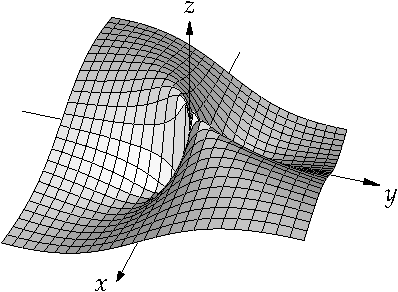
\includegraphics{figures/xyxsqysq}
\caption{Grafik $\frac{xy}{x^2+y^2}$.\label{fig:xyxsqysq}}
\end{myfig}

\begin{example}
Perhatikan
$f \colon X \to \C$ 
pada suatu ruang metrik $X$.
Tuliskan $f(p) = u(p) + i v(p)$, dengan $u \colon X \to \R$
dan $v \colon X \to \R$ sebagai bagian real dan imajinernya.
Maka $f$ kontinu pada $c \in X$ jika dan hanya jika bagian real
dan bagian imajinernya kontinu pada $c$.  
Fakta ini berlaku karena $\bigl\{ f(p_n) = u(p_n) + i v(p_n) \bigr\}_{n=1}^\infty$
konvergen ke $f(p) = u(p) + i v(p)$ jika dan hanya jika
$\bigl\{ u(p_n) \bigr\}$ konvergen ke $u(p)$ dan
$\bigl\{ v(p_n) \bigr\}$ konvergen ke $v(p)$.
\end{example}

\begin{prop}\label{prop:distcont}
Misalkan $(X,d)$ adalah ruang metrik.
\begin{enumerate}[(i)]
\item\label{prop:distcont:i}
Jika $p \in X$,
maka $f \colon X \to \R$ yang didefinisikan
oleh $f(x) = d(x,p)$ bersifat kontinu.
\item\label{prop:distcont:ii}
Diberikan suatu himpunan tak kosong $S \subset X$, fungsi
\begin{equation*}
f(x) = \inf_{p \in S} d(x,p)
\end{equation*}
bersifat kontinu.
\end{enumerate}
\end{prop}

\begin{proof}
Ketaksamaan segitiga terbalik
$\sabs{f(x)-f(y)} = \sabs{d(x,p)-d(y,p)} \leq d(x,y)$
memberikan bagian \ref{prop:distcont:i}.

Untuk \ref{prop:distcont:ii}, karena $S$ tak kosong, $f$
bernilai real.  Ambil $x,y \in X$ dan tanpa mengurangi keumuman, andaikan
bahwa $f(x) > f(y)$.
Untuk sebarang $\epsilon > 0$, terdapat $q$ sedemikian sehingga
$\inf_{p \in S} d(y,p) \geq d(y,q) - \epsilon$.
Menggunakan ketaksamaan ini bersama dengan
$\inf_{p \in S} d(x,p) \leq d(x,q)$ dan
ketaksamaan segitiga terbalik memberikan
\begin{equation*}
f(x)-f(y) =
\inf_{p \in S} d(x,p)
-
\inf_{p \in S} d(y,p)
\leq
%\inf_{p \in S} d(x,p) - d(y,q) + \epsilon 
d(x,q) - d(y,q) + \epsilon 
\leq d(x,y) + \epsilon.
\avoidbreak
\end{equation*}
Karena ketaksamaan itu berlaku untuk setiap $\epsilon$, $f$ kontinu.
\end{proof}

\begin{exbox}
\begin{exercise} \label{exercise:continuousintoperator}
Ambil ruang metrik fungsi-fungsi kontinu $C([0,1],\R)$.  Misalkan
$k \colon [0,1] \times [0,1] \to \R$ adalah fungsi kontinu.
Diberikan $f \in C([0,1],\R)$, definisikan
\begin{equation*}
\varphi_f(x) = \int_0^1 k(x,y) f(y)  \, dy .
\end{equation*}
\begin{exparts}
\item
Tunjukkan bahwa $T(f) = \varphi_f$ mendefinisikan suatu fungsi $T \colon C([0,1],\R) \to
C([0,1],\R)$.
\item
Tunjukkan bahwa $T$ kontinu.
\end{exparts}
\end{exercise}

\begin{exercise} \label{exercise:metriccontinuous}
Misalkan $(X,d)$ adalah ruang metrik.
Definisikan suatu metrik pada $X \times X$ seperti pada bagian b
\exerciseref{exercise:mscross}, dan tunjukkan bahwa $g \colon X \times X \to \R$ yang didefinisikan oleh
$g(x,y) = d(x,y)$ bersifat kontinu.
\end{exercise}

\begin{exercise}
Misalkan $C([a,b],\R)$ adalah himpunan fungsi-fungsi kontinu dan
$C^1([a,b],\R)$ adalah himpunan fungsi-fungsi yang terdiferensialkan
secara kontinu satu kali pada $[a,b]$.
Definisikan
\begin{equation*}
d_{C}(f,g) = \snorm{f-g}_S
\qquad \text{dan} \qquad
d_{C^1}(f,g) = \snorm{f-g}_S + \snorm{f'-g'}_S,
\end{equation*}
di mana $\snorm{\cdot}_S$ adalah norma seragam.
Menurut \exampleref{example:msC01} dan \exerciseref{exercise:C1ab},
$C([a,b],\R)$ dengan $d_C$ adalah ruang metrik, dan demikian pula
$C^1([a,b],\R)$ dengan $d_{C^1}$.
\begin{exparts}
\item
Buktikan bahwa operator turunan $D \colon 
C^1([a,b],\R) \to C([a,b],\R)$ yang didefinisikan oleh
$D(f) = f'$ bersifat kontinu.
\item
Di sisi lain, jika kita menggunakan metrik $d_C$ pada $C^1([a,b],\R)$,
maka buktikan bahwa operator turunan tidak lagi kontinu.  Petunjuk: Perhatikan
$\sin(n x)$.
\end{exparts}
\end{exercise}

\begin{exercise}
Definisikan
\begin{equation*}
f(x,y) =
\begin{cases}
\frac{2xy}{x^4+y^2} & \text{jika } (x,y) \neq (0,0), \\
0 & \text{jika } (x,y) = (0,0) .
\end{cases}
\end{equation*}
\begin{exparts}
\item
Tunjukkan bahwa untuk setiap $y$ yang tetap, fungsi yang memetakan $x$ ke $f(x,y)$
bersifat kontinu dan karenanya terintegralkan Riemann.
\item
Untuk setiap $x$ yang tetap, fungsi yang memetakan $y$ ke $f(x,y)$ bersifat kontinu.
\item
Tunjukkan bahwa $f$ tidak kontinu pada $(0,0)$.
\item
Sekarang tunjukkan bahwa $g(y) = \int_0^1 f(x,y)\,dx$ tidak kontinu pada $y=0$.
\end{exparts}
Catatan: Anda boleh menggunakan apa yang Anda ketahui mengenai $\arctan$ dari kalkulus,
khususnya bahwa $\frac{d}{ds} \bigl[ \arctan(s) \bigr] = \frac{1}{1+s^2}$.
\end{exercise}
\end{exbox}


\subsection{Kekompakan dan kekontinuan}

Pemetaan kontinu tidak memetakan himpunan tertutup ke himpunan tertutup.  Sebagai contoh,
$f \colon (0,1) \to \R$ yang didefinisikan oleh $f(x) = x$ memetakan himpunan $(0,1)$, yang
tertutup dalam $(0,1)$, ke himpunan $(0,1)$, yang tidak tertutup dalam $\R$.
Di sisi lain, pemetaan kontinu mempertahankan himpunan kompak.

\begin{lemma} \label{lemma:continuouscompact}
Misalkan $(X,d_X)$ dan $(Y,d_Y)$ adalah ruang-ruang metrik
dan $f \colon X \to Y$ suatu fungsi kontinu.  Jika
$K \subset X$ adalah himpunan kompak, maka $f(K)$ adalah himpunan kompak.
\end{lemma}

\begin{proof}
Tuliskan
suatu barisan dalam $f(K)$ sebagai
$\bigl\{ f(x_n) \bigr\}_{n=1}^\infty$, di mana
$\{ x_n \}_{n=1}^\infty$ adalah barisan dalam $K$.  Himpunan $K$ kompak, sehingga
terdapat subbarisan
$\{ x_{n_\ell} \}_{\ell=1}^\infty$ yang konvergen ke suatu $x \in K$.
Menurut kekontinuan,
\begin{equation*}
\lim_{\ell\to\infty} f(x_{n_\ell}) = f(x) \in f(K) .
\end{equation*}
Jadi, setiap barisan dalam $f(K)$ mempunyai suatu subbarisan yang konvergen ke 
suatu titik dalam $f(K)$, dan $f(K)$ kompak menurut \thmref{thm:mscompactisseqcpt}.
\end{proof}

Seperti sebelumnya, $f \colon X \to \R$ mencapai suatu
\emph{\myindex{minimum mutlak}} pada $c \in X$ jika
\begin{equation*}
f(x) \geq f(c) \qquad \text{untuk semua } x \in X.
\end{equation*}
Di sisi lain, $f$ mencapai suatu 
\emph{\myindex{maksimum mutlak}} pada $c \in X$ jika
\begin{equation*}
f(x) \leq f(c) \qquad \text{untuk semua } x \in X.
\end{equation*}

\begin{thm}
Misalkan $(X,d)$ adalah ruang metrik kompak tak kosong
dan $f \colon X \to \R$ kontinu.  Maka
$f$ mencapai minimum dan maksimum mutlak pada $X$.
Khususnya, $f$ terbatas.
\end{thm}

\begin{proof}
Karena $X$ kompak dan $f$ kontinu,
$f(X) \subset \R$ kompak.  Oleh karena itu, $f(X)$ tertutup
dan terbatas.  Khususnya,
$\sup f(X) \in f(X)$ dan
$\inf f(X) \in f(X)$, sebab sup maupun inf
dapat dicapai oleh barisan-barisan dalam $f(X)$ dan $f(X)$ tertutup.
Oleh karena itu, terdapat suatu $x \in X$ sedemikian sehingga $f(x) = \sup f(X)$
dan suatu $y \in X$ sedemikian sehingga $f(y) = \inf f(X)$.
\end{proof}

\begin{exbox}
\begin{exercise}
Misalkan $(X,d)$ adalah ruang metrik.
Gunakan \exerciseref{exercise:metriccontinuous} untuk membuktikan bahwa
jika $K_1$ dan $K_2$ adalah subhimpunan kompak dari $X$, maka
terdapat $p \in K_1$ dan $q \in K_2$ sedemikian sehingga $d(p,q)$ minimal,
yakni, $d(p,q) = \inf \{ d(x,y) \colon x \in K_1, y \in K_2 \}$.
\end{exercise}

\begin{exercise}
Misalkan $(X,d)$ adalah ruang metrik kompak, dan misalkan $C(X,\R)$ adalah himpunan
fungsi-fungsi kontinu bernilai real.  Definisikan
\begin{equation*}
d(f,g) = \snorm{f-g}_S = \sup_{x \in X} \abs{f(x)-g(x)} .
\end{equation*}
\begin{exparts}
\item
Tunjukkan bahwa $d$ menjadikan $C(X,\R)$ suatu ruang metrik.
\item
Tunjukkan bahwa untuk setiap $x \in X$, fungsi evaluasi
$E_x \colon C(X,\R) \to \R$ yang didefinisikan oleh $E_x(f) = f(x)$
adalah fungsi kontinu.
\end{exparts}
\end{exercise}
\end{exbox}

\subsection{Kekontinuan dan topologi}

Mari kita lihat cara mendefinisikan kekontinuan dalam istilah topologi, yaitu,
himpunan-himpunan terbuka.  Kita telah melihat bahwa topologi menentukan barisan mana 
yang konvergen, sehingga tidak mengherankan bahwa topologi juga
menentukan kekontinuan fungsi.

\begin{lemma} \label{lemma:mstopocontloc}
Misalkan $(X,d_X)$ dan $(Y,d_Y)$ adalah ruang-ruang metrik.
Suatu fungsi $f \colon X \to Y$ kontinu pada $c \in X$
jika dan hanya jika untuk setiap lingkungan terbuka $U$ dari $f(c)$ dalam $Y$, himpunan
$f^{-1}(U)$ memuat suatu lingkungan terbuka dari $c$ dalam $X$.
Lihat \figureref{fig:mscontfuncpt}.
\end{lemma}

Dengan kata lain, $f^{-1}(U)$ adalah suatu lingkungan dari $c$ yang tidak harus terbuka.

\begin{myfig}
\subimport*{figures/}{mscontfuncpt.pdf_t}
\caption{Untuk setiap lingkungan $U$ dari $f(c)$, himpunan $f^{-1}(U)$ memuat suatu
lingkungan terbuka $W$ dari $c$.\label{fig:mscontfuncpt}}
\end{myfig}

\begin{proof}
Pertama, andaikan $f$ kontinu pada $c$.
Misalkan $U$ adalah lingkungan terbuka dari $f(c)$
dalam $Y$, maka $B_Y\bigl(f(c),\epsilon\bigr) \subset U$ untuk suatu $\epsilon >
0$.  Menurut kekontinuan $f$, terdapat $\delta > 0$
sedemikian sehingga apabila $x$ memenuhi $d_X(x,c) < \delta$, maka
$d_Y\bigl(f(x),f(c)\bigr) < \epsilon$.  Dengan kata lain,
\begin{equation*}
B_X(c,\delta) \subset f^{-1}\bigl(B_Y\bigl(f(c),\epsilon\bigr)\bigr) \subset
f^{-1}(U) ,
\end{equation*}
dan $B_X(c,\delta)$ adalah lingkungan terbuka dari $c$.

Untuk arah sebaliknya,
misalkan diberikan $\epsilon > 0$.  Jika
$f^{-1}\bigl(B_Y\bigl(f(c),\epsilon\bigr)\bigr)$ memuat suatu lingkungan
terbuka $W$ dari $c$, maka himpunan itu memuat suatu bola.  Artinya, terdapat $\delta > 0$
sedemikian sehingga
\begin{equation*}
B_X(c,\delta) \subset W \subset f^{-1}\bigl(B_Y\bigl(f(c),\epsilon\bigr)\bigr) .
\end{equation*}
Hal itu persis berarti bahwa jika $d_X(x,c) < \delta$, maka $d_Y\bigl(f(x),f(c)\bigr)
< \epsilon$, sehingga $f$ kontinu pada $c$.
\end{proof}

\begin{thm} \label{thm:mstopocont}
Misalkan $(X,d_X)$ dan $(Y,d_Y)$ adalah ruang-ruang metrik.  Suatu fungsi $f \colon X \to Y$
kontinu jika dan hanya jika
untuk setiap himpunan terbuka $U \subset Y$, $f^{-1}(U)$ terbuka dalam $X$.
\end{thm}

Bukti ini mengikuti dari \lemmaref{lemma:mstopocontloc} dan diserahkan sebagai
latihan.

\begin{exbox}
\begin{exercise}
Buktikan \thmref{thm:mstopocont}.  Petunjuk: Gunakan \lemmaref{lemma:mstopocontloc}.
\end{exercise}
\end{exbox}


\begin{example}
Misalkan $f \colon X \to Y$ adalah suatu fungsi kontinu.
\thmref{thm:mstopocont} memberi tahu kita bahwa jika $E \subset Y$ tertutup, maka 
$f^{-1}(E) = X \setminus f^{-1}(E^c)$ juga tertutup.  Oleh karena itu,
diberikan
suatu fungsi kontinu $f \colon X \to \R$, 
\emph{\myindex{himpunan nol}} dari $f$, yaitu, 
$f^{-1}(0) = \{ x \in X :
f(x) = 0 \}$, bersifat tertutup.

Himpunan tempat $f$ tak negatif, yaitu,
$f^{-1}\bigl( [0,\infty) \bigr) = \{ x \in X :
f(x) \geq 0 \}$, bersifat tertutup.  Di sisi lain,
himpunan tempat $f$ positif,
$f^{-1}\bigl( (0,\infty) \bigr) = \{ x \in X :
f(x) > 0 \}$, bersifat terbuka.  
\end{example}

\begin{exbox}
\begin{exercise}
Perhatikan $\N \subset \R$ dengan metrik standar.  Misalkan $(X,d)$ adalah suatu
ruang metrik dan $f \colon X \to \N$ suatu fungsi kontinu.
\begin{exparts}
\item
Buktikan bahwa jika $X$ terhubung,
maka $f$ konstan (daerah hasil $f$ hanya terdiri atas satu nilai).
\item
Carilah suatu contoh dengan $X$ tak terhubung dan $f$ tidak konstan.
\end{exparts}
\end{exercise}

\begin{exercise} 
Andaikan $(X,d_X)$, $(Y,d_Y)$ adalah ruang-ruang metrik dan
$f \colon X \to Y$ kontinu.
Misalkan $A \subset X$.
\begin{exparts}
\item
Tunjukkan bahwa $f(\widebar{A}) \subset \overline{f(A)}$.
\item
Tunjukkan bahwa inklusi tersebut dapat bersifat sejati.
\end{exparts}
\end{exercise}

\begin{exercise} \label{exercise:msconnconn}
Andaikan $f \colon X \to Y$ kontinu untuk ruang-ruang metrik $(X,d_X)$
dan $(Y,d_Y)$.  Tunjukkan bahwa jika $X$ terhubung, maka $f(X)$ terhubung.
\end{exercise}

\begin{exercise}
Buktikan versi berikut dari
teorema nilai antara.  Misalkan $(X,d)$ adalah ruang metrik
terhubung dan $f \colon X \to \R$ suatu fungsi kontinu.  Andaikan bahwa
terdapat $x_0,x_1 \in X$ dan $y \in \R$ sedemikian sehingga $f(x_0) < y < f(x_1)$.
Maka buktikan bahwa terdapat $z \in X$ sedemikian sehingga $f(z) = y$.
Petunjuk: Lihat \exerciseref{exercise:msconnconn}.
\end{exercise}

\begin{exercise}
Misalkan $(X,d_X)$ dan $(Y,d_Y)$ adalah ruang-ruang metrik dan
$f \colon X \to Y$ adalah fungsi kontinu satu-ke-satu dan pada.  Andaikan
$X$ kompak.  Buktikan bahwa invers $f^{-1} \colon Y \to X$
bersifat kontinu.
\end{exercise}
\end{exbox}

\subsection{Kekontinuan seragam}

Seperti halnya untuk fungsi-fungsi kontinu
pada garis real, dalam definisi kekontinuan
kadang-kadang lebih mudah jika kita dapat memilih
satu $\delta$ untuk semua titik.

\begin{defn}
Misalkan $(X,d_X)$ dan $(Y,d_Y)$ adalah ruang-ruang metrik.
Maka $f \colon X \to Y$
\emph{kontinu seragam}\index{kontinu seragam}
jika untuk setiap $\epsilon > 0$
terdapat $\delta > 0$ sedemikian sehingga apabila $p,q \in X$ dan $d_X(p,q) <
\delta$, maka
$d_Y\bigl(f(p),f(q)\bigr) < \epsilon$.
\end{defn}

Suatu fungsi kontinu seragam bersifat kontinu, tetapi tidak selalu
sebaliknya.  Pernyataan \myquote{sebaliknya} berlaku jika $X$ kompak.

\begin{thm} \label{thm:Xcompactfunifcont}
Misalkan $(X,d_X)$ dan $(Y,d_Y)$ adalah ruang-ruang metrik.
Andaikan $f \colon X \to Y$ kontinu dan $X$ kompak.  Maka
$f$ kontinu seragam.
\end{thm}

\begin{proof}
Misalkan diberikan $\epsilon > 0$.  Untuk setiap $c \in X$, pilih $\delta_c > 0$ sedemikian sehingga
$d_Y\bigl(f(x),f(c)\bigr) < \nicefrac{\epsilon}{2}$
apabila
$x \in B(c,\delta_c)$.
Bola-bola
$B(c,\delta_c)$ menyelimuti $X$, dan ruang $X$ kompak.  
Terapkan \hyperref[ms:lebesgue]{lemma selimut Lebesgue} untuk memperoleh suatu 
$\delta > 0$ sedemikian sehingga untuk setiap $x \in X$, terdapat $c \in X$
yang memenuhi $B(x,\delta) \subset B(c,\delta_c)$.

Jika $p, q \in X$ dengan $d_X(p,q) < \delta$,
carilah $c \in X$ sedemikian sehingga $B(p,\delta) \subset B(c,\delta_c)$.
Maka $q \in B(c,\delta_c)$.  Menurut ketaksamaan segitiga
dan definisi $\delta_c$,
\begin{equation*}
d_Y\bigl(f(p),f(q)\bigr)
\leq
d_Y\bigl(f(p),f(c)\bigr)
+
d_Y\bigl(f(c),f(q)\bigr)
<
\nicefrac{\epsilon}{2}+
\nicefrac{\epsilon}{2} = \epsilon .  \qedhere
\end{equation*}
\end{proof}


\begin{example}
Contoh-contoh fungsi kontinu seragam yang berguna adalah apa yang disebut
fungsi \emph{kontinu Lipschitz}%
\index{kontinu Lipschitz}%
\index{fungsi!Lipschitz}.
Artinya, jika
$(X,d_X)$ dan $(Y,d_Y)$ adalah ruang-ruang metrik, maka $f \colon X \to Y$
disebut Lipschitz atau $K$-Lipschitz jika terdapat $K \in \R$ sedemikian sehingga
\begin{equation*}
d_Y\bigl(f(p),f(q)\bigr) \leq K d_X(p,q)
\qquad \text{untuk semua } p,q \in X.
\end{equation*}
Suatu fungsi Lipschitz bersifat kontinu seragam:
Ambil $\delta = \nicefrac{\epsilon}{K}$.
Suatu fungsi dapat bersifat kontinu seragam
tetapi tidak Lipschitz:
$\sqrt{x}$ pada $[0,1]$
bersifat kontinu seragam tetapi tidak Lipschitz (latihan).

Patut disebutkan bahwa,
jika suatu fungsi bersifat Lipschitz, biasanya
cara termudah adalah langsung menunjukkan bahwa fungsi itu Lipschitz sekalipun kita hanya
berkepentingan mengetahui kekontinuannya (atau kekontinuan seragamnya).
\end{example}

\begin{exbox}
\begin{exercise}
Tunjukkan bahwa $\sqrt{x}$ kontinu seragam pada $[0,1]$ tetapi tidak Lipschitz.
\end{exercise}

\begin{exercise}
\begin{exparts}
\item
Tunjukkan bahwa $f \colon (c,\infty) \to \R$ untuk suatu $c > 0$
yang didefinisikan oleh $f(x) = \nicefrac{1}{x}$ bersifat kontinu Lipschitz.
\item
Tunjukkan bahwa $f \colon (0,\infty) \to \R$
yang didefinisikan oleh $f(x) = \nicefrac{1}{x}$ tidak kontinu Lipschitz maupun
kontinu seragam.
\end{exparts}
\end{exercise}

\begin{exercise}
Andaikan $f \colon \R \to \R$ adalah suatu fungsi terdiferensialkan
sedemikian sehingga $f'$ adalah fungsi terbatas.  Buktikan bahwa
$f$ adalah fungsi kontinu Lipschitz.
\end{exercise}

\begin{exercise}
Buktikan bahwa pemetaan $T$ yang didefinisikan dalam \exerciseref{exercise:continuousintoperator}
bersifat kontinu Lipschitz.
\end{exercise}

\begin{exercise}
Misalkan $f \colon \R \to \R$ adalah suatu polinom berderajat 
$d \geq 2$.  Tunjukkan bahwa $f$ tidak kontinu
Lipschitz.
\end{exercise}
\end{exbox}

\subsection{Titik klaster dan limit kontinu}

\begin{defn}
Misalkan $(X,d)$ adalah ruang metrik dan
$S \subset X$. Suatu titik $p \in X$ disebut
\emph{titik klaster}\index{titik klaster} dari $S$
jika untuk setiap $\epsilon > 0$, himpunan $B(p,\epsilon) \cap S
\setminus \{ p \}$ tidak kosong.
\end{defn}

\begin{defn}
\index{limit!fungsi dalam ruang metrik}%
Misalkan $(X,d_X)$, $(Y,d_Y)$ adalah ruang-ruang metrik, $S \subset X$, $p \in X$ suatu titik klaster dari $S$,
dan $f \colon S \to Y$ suatu fungsi.
Andaikan terdapat $L \in Y$ dan untuk setiap $\epsilon > 0$,
terdapat $\delta > 0$ sedemikian sehingga apabila $x \in S \setminus \{ p \}$
dan $d_X(x,p) < \delta$, maka
\begin{equation*}
d_Y\bigl(f(x),L\bigr) < \epsilon .
\end{equation*}
Maka $f(x)$
\emph{konvergen}\index{konvergen!fungsi dalam ruang metrik} ke $L$ ketika $x$
menuju $p$, dan $L$ adalah \emph{limit} dari $f(x)$ ketika $x$
menuju $p$.  Kita tuliskan
\glsadd{not:limfunc}%
\begin{equation*}
\lim_{x \to p} f(x) \overset{\text{def}}{=} L .
\end{equation*}
Jika $f(x)$ tidak konvergen ketika $x$ menuju $p$, kita mengatakan bahwa $f$
\emph{divergen}\index{divergen!fungsi dalam ruang metrik} pada $p$.
\end{defn}

Kita kembali menggunakan kata sandang tertentu tanpa menunjukkan bahwa
limit tersebut tunggal.  Bukti ketunggalannya kita serahkan sebagai latihan.

\begin{prop} \label{prop:mslimitisunique}
Misalkan $(X,d_X)$ dan $(Y,d_Y)$ adalah ruang-ruang metrik, $S \subset X$, $p \in X$
suatu titik klaster dari $S$, dan misalkan $f \colon S \to Y$ adalah suatu fungsi
sedemikian sehingga $f(x)$ konvergen ketika $x$ menuju $p$.  Maka
limit dari $f(x)$ ketika $x$ menuju $p$ adalah tunggal.
\end{prop}

\begin{exbox}
\begin{exercise}
Buktikan \propref{prop:mslimitisunique}.
\end{exercise}
\end{exbox}


Dalam ruang metrik, limit kontinu dapat digantikan dengan limit barisan.
Buktinya kita serahkan sebagai latihan.
Intinya, kita sebenarnya hanya perlu membuktikan berbagai hal untuk limit barisan.

\begin{lemma}\label{ms:seqflimit:lemma}
Misalkan $(X,d_X)$ dan $(Y,d_Y)$ adalah ruang-ruang metrik, $S \subset X$, $p \in X$
suatu titik klaster dari $S$, dan misalkan $f \colon S \to Y$ adalah suatu fungsi.

Maka
$f(x)$ konvergen ke $L \in Y$ ketika $x$ menuju $p$ jika dan hanya jika untuk setiap barisan $\{ x_n \}$
dalam $S \setminus \{p\}$
sedemikian sehingga $\lim\, x_n = p$,
barisan $\bigl\{ f(x_n) \bigr\}$ konvergen ke $L$.
\end{lemma}

\begin{exbox}
\begin{exercise}
Buktikan \lemmaref{ms:seqflimit:lemma}.
\end{exercise}
\end{exbox}

Dengan menerapkan \propref{prop:contiscont} atau definisinya secara langsung, kita mendapati
(latihan) bahwa untuk titik klaster $p$ dari $S
\subset X$, fungsi
$f \colon S \to Y$ kontinu pada $p$ jika dan hanya jika
\begin{equation*}
\lim_{x \to p} f(x) = f(p) .
\end{equation*}

\begin{exbox}
\begin{exercise}
Misalkan $(X,d)$ adalah ruang metrik, $S \subset X$, dan $p \in X$.  Buktikan bahwa
$p$ adalah titik klaster dari $S$ jika dan hanya jika $p \in \overline{S \setminus \{
p \}}$.
\end{exercise}

\begin{exercise}
Misalkan $(X,d_X)$ dan $(Y,d_Y)$ adalah ruang-ruang metrik, $S \subset X$, $p \in X$
suatu titik klaster dari $S$, dan misalkan $f \colon S \to Y$ adalah suatu fungsi.
Buktikan bahwa
$f \colon S \to Y$ kontinu pada $p$ jika dan hanya jika
$\lim_{x \to p} f(x) = f(p)$.
\end{exercise}
\end{exbox}

%%%%%%%%%%%%%%%%%%%%%%%%%%%%%%%%%%%%%%%%%%%%%%%%%%%%%%%%%%%%%%%%%%%%%%%%%%%%%%
%%%%%%%%%%%%%%%%%%%%%%%%%%%%%%%%%%%%%%%%%%%%%%%%%%%%%%%%%%%%%%%%%%%%%%%%%%%%%%
%%%%%%%%%%%%%%%%%%%%%%%%%%%%%%%%%%%%%%%%%%%%%%%%%%%%%%%%%%%%%%%%%%%%%%%%%%%%%%

\chapter{Hasil-Hasil dari Analisis Dasar} \label{ap:basicanal}

\begin{myepigraph}
Saya menolak menjawab pertanyaan itu dengan alasan bahwa saya tidak tahu
jawabannya.

---Douglas Adams
\end{myepigraph}

Untuk buku ini,
kita mengasumsikan sebagai prasyarat suatu pengetahuan dasar tentang analisis pada garis real.
Namun, mari kita meninjau beberapa hasil dasar yang mungkin belum
dijumpai pembaca dalam kuliah semacam itu, dan yang berguna dalam teks ini.  Selain itu,
kita memerlukan beberapa hasil ini dalam ruang metrik, dan meskipun bukti-buktinya
pada dasarnya sama seperti pada garis real, hasil-hasil tersebut patut dituliskan.
Teks ini sebagian diadaptasi dari \cite{ra:book} dan \cite{ra:book2}.
Lihat kedua teks tersebut untuk perincian lebih lanjut.

%%%%%%%%%%%%%%%%%%%%%%%%%%%%%%%%%%%%%%%%%%%%%%%%%%%%%%%%%%%%%%%%%%%%%%%%%%%%%%

\section{Barisan fungsi}
\label{sec:puconv}

\subsection{Konvergensi titik demi titik dan seragam serta norma seragam}

Dalam pembahasan berikut, $S$ adalah sebarang himpunan.

\begin{defn}
\index{konvergensi titik demi titik}
Barisan
$\{ f_n \}_{n=1}^\infty$ dari fungsi-fungsi $f_n \colon S \to \R$
\emph{\myindex{konvergen titik demi titik}} ke $f \colon S \to \R$, jika untuk setiap $x
\in S$,
\begin{equation*}
f(x) =
\lim_{n\to\infty} f_n(x) .
\end{equation*}
\end{defn}

Jika kita mengatakan $f_n \colon S \to \R$
\emph{konvergen ke $f$ pada $T \subset S$},
yang kita maksud adalah
restriksi $f_n$ pada $T$ konvergen titik demi titik ke $f$.
Karena limit barisan bilangan bersifat tunggal, fungsi limit $f$ juga tunggal.

Konvergensi titik demi titik tidak mempertahankan banyak struktur pada $f$.
Sebagai contoh, limit titik demi titik dari fungsi-fungsi kontinu tidak harus kontinu;
lihat latihan-latihan.

\begin{defn}
\index{konvergensi seragam}
Misalkan $f_n \colon S \to \R$
dan $f \colon S \to \R$
adalah fungsi-fungsi.  Barisan $\{ f_n \}$
\emph{\myindex{konvergen seragam}} ke $f$, jika untuk
setiap $\epsilon > 0$ terdapat $N \in \N$ sedemikian sehingga 
untuk semua $n \geq N$,
\begin{equation*}
\abs{f_n(x) - f(x)} < \epsilon \qquad \text{untuk semua } x \in S.
\end{equation*}
\end{defn}

Dalam konvergensi seragam, $N$ tidak boleh bergantung pada $x$.  Diberikan $\epsilon > 0$,
kita harus mencari $N$ yang berlaku untuk semua $x \in S$.  Lihat
\figureref{fig:uniformconv} untuk suatu ilustrasi.
Dapat dilihat dengan mudah bahwa konvergensi seragam mengakibatkan konvergensi
titik demi titik.  Implikasinya tidak berlaku sebaliknya.
\begin{myfig}
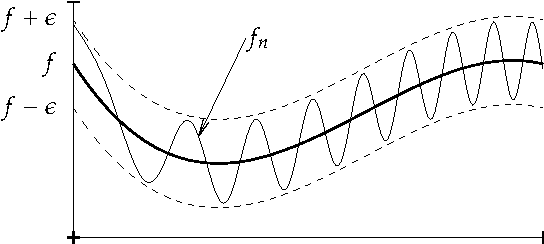
\includegraphics{figures/uniformconv}
\caption{Dalam konvergensi seragam,
untuk $n \geq N$,
fungsi-fungsi $f_n$ berada dalam suatu pita berjarak $\pm\epsilon$ dari $f$.%
\label{fig:uniformconv}}
\end{myfig}

\begin{exbox}
\begin{exercise} \label{exercise:limitnotcont}
Misalkan $f_n(x)=x^n$ adalah fungsi-fungsi pada $[0,1]$.
\begin{exparts}
\item
Tunjukkan bahwa $\{ f_n \}$ konvergen titik demi titik ke suatu fungsi tak kontinu.
\item
Buktikan bahwa $\{ f_n \}$ konvergen
titik demi titik tetapi tidak seragam.
\end{exparts}
\end{exercise}

\begin{exercise}
Andaikan $f_n \colon S \to \R$ adalah fungsi-fungsi yang konvergen seragam
ke $f \colon S \to \R$.  Andaikan $A \subset S$.  Tunjukkan bahwa
barisan restriksi $\{ f_n|_A \}$ konvergen seragam ke $f|_A$.
\end{exercise}

\begin{exercise}
\begin{exparts}
\item
Andaikan $\{ f_n \}$ dan $\{ g_n \}$ yang didefinisikan pada suatu himpunan $A$ masing-masing
konvergen titik demi titik ke $f$ dan $g$.
Untuk $a,b \in \R$,
tunjukkan bahwa $\{ a f_n+ b g_n \}$ konvergen titik demi titik ke $a f+ b g$.
\item
Tunjukkan hal yang sama untuk konvergensi seragam.
\end{exparts}
\end{exercise}

\begin{exercise}
Carilah suatu contoh barisan fungsi $\{ f_n \}$ dan $\{ g_n \}$
yang konvergen seragam ke suatu $f$ dan $g$ pada suatu himpunan $A$, tetapi sedemikian sehingga
$\{ f_ng_n \}$ (hasil kalinya) tidak konvergen seragam ke $fg$ pada $A$.
\end{exercise}

\begin{exercise}
Andaikan terdapat suatu barisan fungsi $\{ g_n \}$ yang konvergen seragam
ke $0$ pada $A$.  Sekarang andaikan kita mempunyai suatu barisan fungsi
$\{ f_n \}$ dan suatu fungsi $f$ pada $A$ sedemikian sehingga
\begin{equation*}
\abs{f_n(x) - f(x)} \leq g_n(x) 
\end{equation*}
untuk semua $x \in A$.  Tunjukkan bahwa $\{ f_n \}$ konvergen seragam ke $f$ pada $A$.
\end{exercise}

\begin{exercise}
Misalkan $\{ f_n \}$, $\{ g_n \}$, dan $\{ h_n \}$ adalah barisan-barisan fungsi pada
suatu himpunan $S$.
Andaikan $\{ f_n \}$ dan $\{ h_n \}$ konvergen seragam ke suatu fungsi
$f \colon S \to \R$ dan andaikan $f_n(x) \leq g_n(x) \leq h_n(x)$
untuk semua $x \in S$.  Tunjukkan bahwa $\{ g_n \}$ konvergen seragam ke $f$.
\end{exercise}

\begin{exercise}
Buktikan bahwa
jika suatu barisan fungsi $f_n \colon S \to \R$
konvergen seragam ke suatu fungsi terbatas $f \colon S \to \R$,
maka terdapat $N$ sedemikian sehingga untuk semua $n \geq N$, fungsi-fungsi $f_n$
terbatas.
\end{exercise}
\end{exbox}

\begin{defn} \label{def:unifnorm}
Untuk $f \colon S \to \R$, definisikan
\emph{\myindex{norma seragam}},
\glsadd{not:uniformnorm}%
\begin{equation*}
\snorm{f}_S
\overset{\text{def}}{=}
\sup \bigl\{ \sabs{f(x)} : x \in S \bigr\} .
\end{equation*}
\end{defn}

Perhatikan bahwa jika $f$ tidak terbatas, maka $\snorm{f}_S = \infty$.  Oleh karena itu,
kecuali jika berurusan dengan fungsi-fungsi terbatas, kita memperlakukan norma tersebut sebagai bilangan real diperluas,
sehingga ini bukan apa yang orang sebut suatu \myquote{norma} kecuali jika kita membatasi pada fungsi-fungsi terbatas.

\begin{prop}
Suatu barisan $f_n \colon S \to \R$ konvergen
seragam ke $f \colon S \to \R$ jika dan hanya jika
\begin{equation*}
\lim_{n\to\infty} \snorm{f_n - f}_S = 0 .
\end{equation*}
\end{prop}

\begin{exbox}
\begin{exercise}
Buktikan proposisi tersebut.
\end{exercise}
\end{exbox}

Kita dapat mengatakan
\emph{$\{ f_n \}$ konvergen ke $f$ dalam norma seragam}
\index{konvergen dalam norma seragam}%
\index{konvergensi norma seragam}%
sebagai ganti \emph{konvergen seragam}.  Proposisi tersebut
mengatakan bahwa kedua pengertian itu sama.
Secara umum, cara termudah untuk memikirkan konvergensi seragam fungsi
adalah dengan menggunakan ruang metrik.
Suatu barisan Cauchy fungsi dalam norma seragam dikatakan
\emph{\myindex{Cauchy dalam norma seragam}} atau
\emph{\myindex{Cauchy seragam}}.

\begin{prop}
Himpunan fungsi-fungsi terbatas bernilai real pada $S$ adalah ruang metrik lengkap dengan
metrik $d(f,g) = \snorm{f-g}_S$.
Khususnya, jika suatu barisan adalah Cauchy seragam, maka barisan itu
konvergen seragam.
\end{prop}

\begin{exbox}
\begin{exercise}
Buktikan proposisi tersebut.  Ada dua hal yang harus dibuktikan.  Pertama,
buktikan bahwa himpunan itu adalah ruang metrik, yaitu, $d(f,g)$ adalah suatu metrik.
Kedua, buktikan bahwa ruang itu lengkap.
\end{exercise}
\end{exbox}

\begin{remark}
Barangkali mengejutkan bahwa pada himpunan fungsi $f \colon S \to
\R$ untuk $S$ yang tak terhitung, tidak ada metrik yang menghasilkan konvergensi titik demi titik.
Bahkan jika Anda mensyaratkan $f$ terbatas dan/atau kontinu, tetap
tidak ada metrik demikian.
Suatu ruang metrik $(X,d)$ disebut \emph{\myindex{terhitung pertama}},
yakni, pada setiap $x \in X$ terdapat suatu barisan lingkungan $U_j$ sedemikian
sehingga sebarang lingkungan $U$ dari $x$ memuat salah satu $U_j$, yang disebut
basis lingkungan terhitung.  Dalam ruang metrik, $B(x,\nicefrac{1}{n})$
memenuhi keperluan itu.  Akan tetapi, fungsi-fungsi pada suatu himpunan tak terhitung $S$ dengan konvergensi
titik demi titik tidak mempunyai topologi terhitung pertama.  Kita tidak ingin
menyelami topologi umum terlalu jauh untuk membuktikan fakta ini.
\end{remark}

\subsection{Kekontinuan limit}

Jika kita mempunyai suatu barisan $\{ f_n \}$ dari fungsi-fungsi kontinu,
apakah limitnya kontinu?  Kita telah melihat bahwa untuk konvergensi
titik demi titik, hal itu belum tentu terjadi; lihat \exerciseref{exercise:limitnotcont}.
Namun, jika kita mensyaratkan konvergensinya seragam, limit-limit dapat
dipertukarkan.

\begin{thm} \label{thm:uniformlimitcont}
Misalkan $S$ adalah ruang metrik.
Misalkan $\{ f_n \}$ adalah 
suatu barisan fungsi kontinu $f_n \colon S \to \R$ yang konvergen
seragam ke $f \colon S \to \R$.  Maka $f$ kontinu.
\end{thm}

\begin{proof}
Tetapkan $x \in S$.  Misalkan $\{ x_n \}$ adalah suatu barisan dalam $S$
yang konvergen ke $x$.
Misalkan diberikan $\epsilon > 0$.
Karena $\{ f_k \}$ konvergen seragam ke $f$, kita memperoleh suatu $k \in \N$ sedemikian sehingga
\begin{equation*}
\abs{f_k(y)-f(y)} < \nicefrac{\epsilon}{3}
\end{equation*}
untuk semua $y \in S$.  Karena $f_k$ kontinu pada $x$,
kita memperoleh $N \in \N$ sedemikian sehingga untuk $m \geq N$
berlaku 
\begin{equation*}
\abs{f_k(x_m)-f_k(x)} < \nicefrac{\epsilon}{3} .
\end{equation*}
Dengan demikian, untuk
$m \geq N$,
\begin{equation*}
\begin{split}
\abs{f(x_m)-f(x)}
& =
\abs{f(x_m)-f_k(x_m)+f_k(x_m)-f_k(x)+f_k(x)-f(x)}
\\
& \leq
\abs{f(x_m)-f_k(x_m)}+
\abs{f_k(x_m)-f_k(x)}+
\abs{f_k(x)-f(x)}
\\
& <
\nicefrac{\epsilon}{3} +
\nicefrac{\epsilon}{3} +
\nicefrac{\epsilon}{3} = \epsilon .
\end{split}
\end{equation*}
Oleh karena itu, $\{ f(x_m) \}$ konvergen ke $f(x)$ dan karenanya $f$ kontinu pada
$x$.  Karena $x$ dipilih sembarang, $f$ kontinu di mana-mana.
\end{proof}

Dalam bahasa ruang metrik,
karena limit seragam dari fungsi-fungsi kontinu bersifat kontinu,
himpunan fungsi kontinu terbatas adalah ruang metrik lengkap.
Buktinya diserahkan sebagai latihan.
Lebih tepatnya,
misalkan $C_b(S,\R)$ menyatakan himpunan fungsi kontinu terbatas bernilai real pada $S$.
Kita menggunakan norma seragam sebagai metrik, dan $C_b(S,\R)$ adalah ruang metrik
untuk sebarang $S$.  Jika $S$ kompak, maka semua fungsi kontinu terbatas
dan $C(S,\R)$ sendiri adalah ruang metrik.

\begin{cor} \label{cor:CSRcomplete}
Misalkan $S$ adalah ruang metrik.  Maka $C_b(S,\R)$ adalah ruang metrik lengkap.
Jika $S$ kompak, maka $C(S,\R)$ adalah ruang metrik lengkap.
\end{cor}

\begin{exbox}
\begin{exercise}%[\neededexmark]
Buktikan \corref{cor:CSRcomplete}.
\end{exercise}
\end{exbox}

\begin{defn}
Suatu barisan fungsi $f_n \colon S \to \R$
\emph{\myindex{konvergen seragam pada subhimpunan kompak}}
\index{konvergensi seragam pada subhimpunan kompak}
jika untuk setiap $K \subset S$ yang kompak,
barisan $\{ f_n \}$ konvergen seragam pada $K$.
\end{defn}

\begin{cor} \label{cor:uniformkptlimitcont}
Misalkan $U \subset \R^n$ terbuka.
Jika $f_n \colon U \to \R$ adalah suatu barisan
fungsi kontinu yang konvergen seragam pada subhimpunan kompak, maka
limitnya kontinu.
\end{cor}

\begin{exbox}
\begin{exercise}
Buktikan akibat tersebut.
\end{exercise}
\end{exbox}

\subsection{Integral limit}

Seperti halnya kekontinuan, jika kita hanya mensyaratkan konvergensi titik demi titik, maka integral
dari limit suatu barisan fungsi tidak harus sama dengan limit
dari integral-integralnya.

\begin{example}
Misalkan $\chi_{T}$ adalah fungsi karakteristik suatu himpunan $T$, yaitu, $\chi_T(x) =
1$ jika $x \in T$ dan $\chi_T(x) = 0$ jika tidak.
Semua fungsi $n \chi_{(0,\nicefrac{1}{n})}$ berintegral (pada interval
$[0,1]$) sama dengan $1$.  Limit titik demi titiknya adalah $0$ (yang integralnya $0$).
\end{example}

Jika kita mensyaratkan konvergensinya seragam, limit-limit tersebut dapat
dipertukarkan.

\begin{thm} \label{integralinterchange:thm}
Misalkan $\{ f_n \}$ adalah suatu barisan fungsi yang terintegralkan
Riemann
$f_n \colon [a,b] \to \R$
yang konvergen seragam ke $f \colon [a,b]
\to \R$.  Maka $f$ terintegralkan Riemann dan
\begin{equation*}
\int_a^b f(x) \, dx = \lim_{n\to\infty} \int_a^b f_n(x) \, dx .
\end{equation*}
\end{thm}

Dalam pembahasan berikut, misalkan 
$\overline{\int_a^b} f(x)\, dx$ dan 
$\underline{\int_a^b} f(x)\, dx$ menyatakan integral Darboux atas dan bawah.
Secara ringkas,
\begin{align*}
& \overline{\int_a^b} f(t) \,dt
\overset{\text{def}}{=}
\inf \left\{ \int_a^b s(t) \, dt : s
\text{ adalah fungsi tangga dan } f(t) \leq s(t) \text{ untuk } t \in
[a,b] \right\} ,
\\
& \underline{\int_a^b} f(t) \,dt
\overset{\text{def}}{=}
\sup \left\{ \int_a^b s(t) \, dt : s
\text{ adalah fungsi tangga dan } s(t) \leq f(t) \text{ untuk } t \in
[a,b] \right\} .
\end{align*}


Definisi integral Riemann dengan menggunakan jumlah dan integral Darboux
berada di luar cakupan buku ini, tetapi cukup kita sebutkan bahwa 
jika integral Darboux atas dan bawah sama, maka suatu fungsi
terintegralkan Riemann, dan nilai bersama tersebut adalah integralnya.  Dengan fakta ini,
mari kita buktikan teoremanya.

\begin{proof}
Misalkan diberikan $\epsilon > 0$.
Karena $f_n$ menuju $f$ secara seragam, kita memperoleh $M \in \N$ sedemikian sehingga
untuk semua $n \geq M$, berlaku 
$\abs{f_n(x)-f(x)} < \frac{\epsilon}{2(b-a)}$ untuk semua $x \in [a,b]$.
Khususnya, menurut ketaksamaan segitiga terbalik,
$\abs{f(x)} < \frac{\epsilon}{2(b-a)} + \abs{f_n(x)}$ untuk semua $x$,
sehingga $f$ terbatas
karena $f_n$ terbatas.
Perhatikan bahwa $f_n$ terintegralkan, dan hitung
\begin{align*}
\overline{\int_a^b} & f(x) \, dx
-
\underline{\int_a^b} f(x) \, dx
\\
& =
\overline{\int_a^b} \bigl( f(x) - f_n(x) + f_n(x) \bigr) \, dx
-
\underline{\int_a^b} \bigl( f(x) - f_n(x) + f_n(x) \bigr) \, dx
\displaybreak[0]\\
& \leq
\overline{\int_a^b} \bigl( f(x) - f_n(x) \bigr) \, dx +  \overline{\int_a^b}
f_n(x) \, dx
-
\underline{\int_a^b} \bigl( f(x) - f_n(x) \bigr) \, dx -
\underline{\int_a^b} f_n(x) \, dx
\displaybreak[0]\\
& =
\overline{\int_a^b} \bigl( f(x) - f_n(x) \bigr)\, dx +  \int_a^b f_n(x) \, dx
-
\underline{\int_a^b} \bigl( f(x) - f_n(x) \bigr)\, dx -  \int_a^b f_n(x) \, dx
\displaybreak[0]\\
& =
\overline{\int_a^b} \bigl( f(x) - f_n(x) \bigr)\, dx
-
\underline{\int_a^b} \bigl( f(x) - f_n(x) \bigr)\, dx
\\
& \leq
\frac{\epsilon}{2(b-a)} (b-a) + 
\frac{\epsilon}{2(b-a)} (b-a) = \epsilon .
\end{align*}
Ketaksamaan pertama
berasal dari integral atas yang
hanya subaditif ($\overline{\int} (a+b) \leq \overline{\int}a +
\overline{\int} b$) dan integral bawah yang superaditif.
Ketaksamaan terakhir mengikuti dari
fakta bahwa untuk semua $x \in [a,b]$, berlaku
$\frac{-\epsilon}{2(b-a)} < f(x)-f_n(x) < \frac{\epsilon}{2(b-a)}$.
Karena $\epsilon > 0$ dipilih sembarang, $f$ terintegralkan Riemann.

Kita hitung $\int_a^b f(x)\,dx$.
Untuk $n \geq M$ ($M$ sama seperti di atas),
\begin{equation*}
\begin{split}
\abs{\int_a^b f(x)\,dx - \int_a^b f_n(x) \, dx} & = 
\abs{\int_a^b \bigl(f(x) - f_n(x)\bigr) \, dx}
\\
& \leq
\frac{\epsilon}{2(b-a)} (b-a) = \frac{\epsilon}{2} < \epsilon .
\end{split}
\end{equation*}
Oleh karena itu, $\bigl\{ \int_a^b f_n(x) \,dx \bigr\}$ konvergen ke $\int_a^b f(x) \,dx$.
\end{proof}

\begin{remark}
Walaupun kita tidak memerlukan integral Lebesgue dalam buku ini, perhatikan bahwa
untuk integral Lebesgue berlaku teorema konvergensi yang jauh lebih kuat.  Secara
khusus, teorema konvergensi terdominasi menyatakan bahwa jika
$\{ f_n \}$ adalah suatu barisan fungsi terukur pada $[a,b]$,
yang konvergen titik demi titik ke $f \colon [a,b] \to \R$, dan sedemikian sehingga
$\{ f_n \}$ terbatas seragam (terdapat satu $B \in \R$ sedemikian sehingga
$\snorm{f_n}_{[a,b]} \leq B$ untuk semua $n$), maka
\begin{equation*}
\int_a^b f(x) \, dx = \lim_{n\to\infty} \int_a^b f_n(x) \, dx .
\end{equation*}
Di sini, tentu saja, integral-integralnya harus berupa integral Lebesgue,
bukan integral Riemann.  Limit titik demi titik dari fungsi-fungsi yang terintegralkan
Riemann bahkan tidak harus terintegralkan Riemann.
\end{remark}

\begin{exbox}
\begin{exercise}
Hitunglah
$\displaystyle \lim_{n\to\infty} \int_1^2 e^{-nx^2} \,dx$.
\end{exercise}

\begin{exercise}
Carilah suatu barisan fungsi terintegralkan Riemann $f_n \colon [0,1] \to \R$ sedemikian
sehingga $\{ f_n \}$ konvergen ke nol titik demi titik, dan sedemikian sehingga
\begin{exparts}
\item
$\bigl\{ \int_0^1 f_n(x)\,dx \bigr\}_{n=1}^\infty$ meningkat tanpa batas,
\item
$\bigl\{ \int_0^1 f_n(x)\,dx \bigr\}_{n=1}^\infty$ adalah barisan $-1,1,-1,1,-1,1, \ldots$.
\end{exparts}
\end{exercise}
\end{exbox}

\subsection{Turunan limit}

Konvergensi seragam cukup untuk mempertukarkan limit dengan integral.
Namun, hal itu
tidak cukup untuk mempertukarkan limit dengan turunan, kecuali jika
turunan-turunannya sendiri konvergen seragam.

\begin{example}
Fungsi-fungsi $f_n(x) = \frac{\sin(nx)}{n}$
konvergen seragam ke $0$.
Lihat \figureref{fig:conv1nsinxn}.
Turunan limitnya adalah $0$.
Namun, $f_n'(x) = \cos(nx)$,
dan barisan itu bahkan tidak konvergen titik demi titik:
Sebagai contoh, $f_n'(\pi) = {(-1)}^n$.
Selain itu, $f_n'(0) = 1$ untuk semua $n$, yang memang konvergen, tetapi tidak ke $0$.
\begin{myfig}
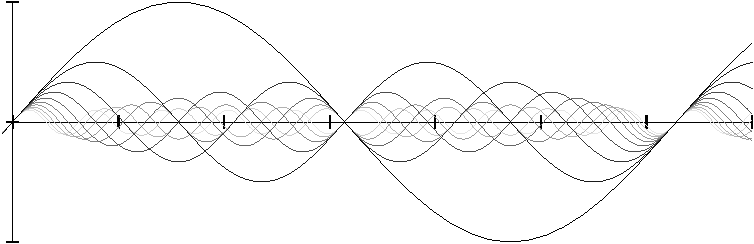
\includegraphics{figures/conv1nsinxn}
\caption{Grafik $\frac{\sin(nx)}{n}$ untuk
$n=1,2,\ldots,10$, dengan $n$ yang lebih besar digambar dalam warna abu-abu yang lebih terang.%
\label{fig:conv1nsinxn}}
\end{myfig}
\end{example}

Teorema berikut tetap benar sekalipun 
kita tidak mengasumsikan kekontinuan turunan-turunannya, tetapi buktinya lebih
sulit.

\begin{thm} \label{thm:dersconverge}
Misalkan $I$ adalah interval terbatas dan
$f_n \colon I \to \R$ adalah fungsi-fungsi yang terdiferensialkan secara kontinu.
Andaikan $\{ f_n' \}$ konvergen seragam ke $g \colon I \to \R$,
dan andaikan $\{ f_n(c) \}_{n=1}^\infty$ adalah suatu
barisan konvergen untuk suatu $c \in I$.  Maka $\{ f_n \}$ konvergen seragam ke 
suatu fungsi yang terdiferensialkan secara kontinu $f \colon I \to \R$, dan $f' = g$.
\end{thm}

\begin{proof}
Definisikan $f(c) = \lim_{n\to \infty} f_n(c)$.
Karena $f_n'$ kontinu dan karenanya terintegralkan Riemann,
melalui teorema dasar kalkulus, kita memperoleh bahwa untuk $x \in I$,
\begin{equation*}
f_n(x) = f_n(c) + \int_c^x f_n' (t)\, dt.
\end{equation*}
Karena $\{ f_n' \}$ konvergen seragam pada $I$, barisan itu konvergen seragam
pada $[c,x]$ (atau $[x,c]$ jika $x < c$).
Dengan demikian, limit di ruas kanan ada.
Definisikan $f$ pada titik-titik sisanya dengan
\begin{equation*}
f(x) =
\lim_{n\to\infty} f_n(c) + \lim_{n\to\infty} \int_c^x f_n' (t)\, dt
=
f(c) + \int_c^x g(t)\,dt .
\end{equation*}
Fungsi $g$ kontinu, karena merupakan limit seragam dari fungsi-fungsi
kontinu.  Oleh karena itu, $f$ terdiferensialkan dan $f'(x) = g(x)$ untuk semua $x \in I$
menurut teorema dasar kalkulus.

Tinggal membuktikan
konvergensi seragam.
Andaikan $I$ mempunyai batas bawah $a$ dan batas atas $b$.
Misalkan diberikan $\epsilon > 0$.  Ambil $M$
sedemikian sehingga untuk $n \geq M$, berlaku
$\abs{f(c)-f_n(c)} < \nicefrac{\epsilon}{2}$
dan
$\abs{g(x)-f_n'(x)} < \frac{\epsilon}{2(b-a)}$
untuk semua $x \in I$.  Maka,
\begin{equation*}
\begin{split}
\abs{f(x) - f_n(x)} & =
\abs{f(c) + \int_c^x g(t) \, dt - f_n(c) - \int_c^x f_n'(t)\,dt}
\\
& \leq
\abs{f(c) - f_n(c)} + \abs{\int_c^x g(t)\,dt - \int_c^x f_n'(t)\,dt}
\\
& =
\abs{f(c) - f_n(c)} + \abs{\int_c^x \bigl(g(t) - f_n'(t)\bigr) \, dt}
\\
& <
\frac{\epsilon}{2}
+
\frac{\epsilon}{2(b-a)}
(b-a)
=\epsilon. \qedhere
\end{split}
\end{equation*}
\end{proof}

Bukti tersebut tetap berlaku tanpa keterbatasan $I$, kecuali untuk
konvergensi seragam $f_n$ ke $f$.  Sebagai contoh, misalkan $I = \R$ dan
$f_n(x) = \nicefrac{x}{n}$.  Maka $f_n'(x)=\nicefrac{1}{n}$, yang
konvergen seragam ke $0$.  Namun, $\{f_n\}$ konvergen ke $0$ hanya titik demi titik.

\begin{example}
Dalam \exerciseref{exercise:C1ab}, Anda membuktikan bahwa
himpunan fungsi-fungsi yang terdiferensialkan secara kontinu satu kali pada $[a,b]$, yaitu,
$C^1([a,b],\R)$, adalah ruang metrik dengan apa yang disebut
metrik $C^1$ (atau norma $C^1$)
\begin{equation*}
d(f,g) =
\snorm{f-g}_{C^1([a,b],\R)}
\overset{\text{def}}{=}
\snorm{f-g}_{[a,b]} + \snorm{f'-g'}_{[a,b]}.
\end{equation*}
Teorema tersebut mengatakan bahwa $C^1([a,b],\R)$ adalah ruang metrik lengkap.
\end{example}

\begin{exbox}
\begin{exercise}
Carilah suatu contoh eksplisit dari suatu barisan
fungsi terdiferensialkan pada $[-1,1]$ yang konvergen seragam ke
suatu fungsi $f$ sedemikian sehingga $f$ tidak terdiferensialkan.
Petunjuk:
Mungkin $\sqrt{x^2+{(\nicefrac{1}{n})}^2}$?
\end{exercise}

\begin{exercise}
Misalkan $f_n(x) = \frac{x^n}{n}$.  Tunjukkan bahwa $\{ f_n \}$ konvergen seragam ke
suatu fungsi terdiferensialkan $f$ pada $[0,1]$ (carilah $f$).  Namun, tunjukkan bahwa
$f'(1) \neq \lim\limits_{n\to\infty} f_n'(1)$.
\end{exercise}
\end{exbox}

%%%%%%%%%%%%%%%%%%%%%%%%%%%%%%%%%%%%%%%%%%%%%%%%%%%%%%%%%%%%%%%%%%%%%%%%%%%%%%

\section{Kekontinuan, Fubini, turunan di bawah integral}
\label{sec:contlimitsunderint}

\subsection{Kekontinuan}

Misalkan $f(x,y)$ adalah fungsi dua variabel dan definisikan
\begin{equation*}
g(y) = \int_a^b f(x,y) \,dx .
\end{equation*}
Pertanyaannya adalah: Apakah $g$ kontinu?
Sesungguhnya kita menanyakan kapan dua limit dapat dipertukarkan,
yang tidak selalu mungkin, sehingga suatu hipotesis tambahan
diperlukan.  Suatu syarat yang cukup (tetapi tidak
perlu) adalah bahwa $f$ kontinu pada persegi panjang tertutup.

\begin{prop} \label{prop:integralcontcont}
Jika $f \colon [a,b] \times [c,d] \to \R$ kontinu,
maka $g \colon [c,d] \to \R$ yang didefinisikan oleh
\begin{equation*}
g(y) = \int_a^b f(x,y) \,dx  \qquad \text{bersifat kontinu}.
\end{equation*}
\end{prop}

\begin{proof}
Tetapkan $y \in [c,d]$, dan misalkan $\{ y_n \}$ adalah suatu barisan dalam $[c,d]$
yang konvergen ke $y$.
Misalkan diberikan $\epsilon > 0$.
Karena $f$ kontinu pada himpunan kompak $[a,b] \times [c,d]$, maka $f$
kontinu seragam.  
Dengan demikian, terdapat $\delta > 0$ sedemikian sehingga
apabila $\widetilde{y} \in [c,d]$ dan
$\abs{\widetilde{y}-y} < \delta$, berlaku
$\abs{f(x,\widetilde{y})-f(x,y)} < \frac{\epsilon}{b-a}$ untuk semua $x \in [a,b]$.
Andaikan $\abs{\widetilde{y}-y} < \delta$.  Maka
\begin{multline*}
\abs{
g(\widetilde{y})-
g(y)
}
=
\bbabs{
\int_a^b 
f(x,\widetilde{y}) \,dx 
-
\int_a^b 
f(x,y) \,dx 
}
\\
=
\bbabs{
\int_a^b 
\bigl(
f(x,\widetilde{y}) - f(x,y)
\bigr)
\,dx 
}
\leq
(b-a)
\frac{\epsilon}{b-a}
= \epsilon . \qedhere
\end{multline*}
\end{proof}

Dalam penerapan, jika kita berkepentingan dengan kekontinuan pada $y_0$, kita hanya
perlu menerapkan proposisi tersebut dalam $[a,b] \times [y_0-\epsilon,y_0+\epsilon]$
untuk suatu $\epsilon > 0$ yang kecil.  Sebagai contoh, jika $f$ kontinu dalam
$[a,b] \times \R$, maka $g$ kontinu pada $\R$.

\begin{exbox}
\begin{exercise} \label{exercise:integralcontcontextra}
Buktikan versi yang lebih kuat dari \propref{prop:integralcontcont}:
Jika $f \colon (a,b) \times (c,d) \to \R$ adalah suatu fungsi kontinu terbatas,
maka $g \colon (c,d) \to \R$ yang didefinisikan oleh
\begin{equation*}
g(y) = \int_a^b f(x,y) \,dx  \qquad \text{bersifat kontinu}.
\end{equation*}
Petunjuk: Pertama-tama integralkan pada $[a+\nicefrac{1}{n},b-\nicefrac{1}{n}]$.
\end{exercise}
\end{exbox}

\subsection{Teorema Fubini}

Teorema Fubini mengatakan bahwa dalam beberapa syarat ringan, secara umum kita dapat
mempertukarkan urutan integral dalam suatu integral berulang.
Kita membuktikan kasus sederhana Fubini berikut, yang secara umum
cukup untuk keperluan buku ini.

\begin{thm}[Fubini]\index{teorema Fubini}\label{thm:fubini}
Andaikan $f \colon [a,b] \times [c,d] \to \R$ kontinu.  Maka
\begin{equation*}
\int_c^d \int_a^b f(x,y) \, dx \, dy =
\int_a^b \int_c^d f(x,y) \, dy \, dx .
\end{equation*}
\end{thm}

Salah satu bagian yang rumit mengenai Fubini untuk integral Riemann
adalah bahwa integran dari integral luar, misalnya
$\int_a^b f(x,y) \, dx$ sebagai fungsi dari $y$, tidak harus 
terintegralkan Riemann sekalipun $f(x,y)$ terintegralkan Riemann sebagai fungsi
dua variabel.  Namun, menurut subbagian sebelumnya, jika $f$ kontinu,
maka $\int_a^b f(x,y) \, dx$ adalah fungsi kontinu dari $y$ dan karenanya
terintegralkan.  Jadi, untuk fungsi kontinu kita menghindari persoalan
keterintegralan.\footnote{Untuk skenario yang lebih rumit, pembaca
dianjurkan untuk mempelajari integral Lebesgue saja.}

\begin{proof}
Karena $[a,b] \times [c,d]$ kompak, $f$ kontinu seragam.
Jadi, untuk
sebarang $\epsilon > 0$, terdapat $\delta > 0$ sedemikian sehingga jika
$\sabs{x-x'} < \delta$ dan 
$\sabs{y-y'} < \delta$, maka $\sabs{f(x,y) -f(x',y')} < \epsilon$.
Misalkan
\begin{equation*}
g_n(x,y)
=
\begin{cases}
f(a,y) & \text{jika } x=a ,
\\
f\left(a+\frac{k(b-a)}{n},y\right)
& \text{jika } a+\frac{(k-1)(b-a)}{n} < x \leq a+\frac{k(b-a)}{n} , ~
k=1,\ldots,n.
\end{cases}
\end{equation*}
Fungsi $g_n$ ini adalah fungsi tangga \myquote{kaidah titik ujung kanan} dengan
panjang subinterval $\frac{b-a}{n}$:
Mengintegralkan $g_n$ terhadap $x$ merupakan kaidah titik ujung kanan untuk mengintegralkan $f$.
Ambil $n$ cukup besar sedemikian sehingga $\frac{b-a}{n} < \delta$.  Maka,
melalui taksiran kekontinuan seragam, kita memperoleh bahwa $\babs{f(x,y)-g_n(x,y)} < \epsilon$
untuk semua $x$ dan $y$. Jadi,
\begin{equation*}
\abs{
\int_a^b
f(x,y)
\, dx
-
\int_a^b
g_n(x,y)
\, dx
}
\leq
\int_a^b
\babs{
f(x,y)
-
g_n(x,y)
}
\, dx
\leq (b-a)\epsilon .
\end{equation*}
Jadi, $\int_a^b g_n(x,y) \, dx$ konvergen seragam sebagai fungsi dari $y$ ke
$\int_a^b f(x,y) \, dx$.  Akhirnya, integral dari $g_n$ hanyalah
kaidah titik ujung kanan.  Dengan menggabungkan semuanya,
\begin{equation*}
\begin{split}
\int_c^d \int_a^b f(x,y) \, dx \, dy
& =
\int_c^d
\left(
\lim_{n \to \infty}
\int_a^b g_n(x,y) \, dx
\right) \, dy
\\
& =
\lim_{n \to \infty}
\int_c^d
\left(
\int_a^b g_n(x,y) \, dx
\right) \, dy
\\
& =
\lim_{n \to \infty}
\int_c^d
\left(
\sum_{k=1}^n
\frac{b-a}{n} f\left(a+\frac{k(b-a)}{n},y\right)
\right) \, dy
\\
& =
\lim_{n \to \infty}
\sum_{k=1}^n
\frac{b-a}{n} 
\int_c^d
f\left(a+\frac{k(b-a)}{n},y\right)
\, dy
\\
& =
\int_a^b
\int_c^d
f(x,y)
\, dy \, dx .
\end{split}
\end{equation*}
Persamaan terakhir hanyalah pengamatan bahwa  
$\int_c^d
f(x,y)
\, dy$ adalah fungsi kontinu dari $x$, sehingga terintegralkan, dan yang kita miliki
hanyalah kaidah titik ujung kanan untuk integral fungsi ini pada $[a,b]$.
\end{proof}

\begin{exbox}
\begin{exercise}
Andaikan $f(x,y) = 1$ jika $x \in \Q$ dan $y=\nicefrac{1}{2}$, dan $0$ jika tidak.
Dengan menggunakan integral Riemann, buktikan bahwa salah satu dari
$\int_0^1 \int_0^1 f(x,y) \, dx \, dy$ dan
$\int_0^1 \int_0^1 f(x,y) \, dy \, dx$ ada dan yang lainnya tidak (integrannya
bukan fungsi yang terdefinisi dengan baik).
\end{exercise}

\begin{exercise}
Hitunglah
\begin{equation*}
\int_0^1 \int_0^1 \frac{x^2-y^2}{{(x^2+y^2)}^2} \, dx \, dy
\qquad \text{dan} \qquad
\int_0^1 \int_0^1 \frac{x^2-y^2}{{(x^2+y^2)}^2} \, dy \, dx .
\end{equation*}
Anda perlu menafsirkan integral-integral tersebut sebagai integral tak wajar, yaitu,
limit dari $\int_\epsilon^1$ ketika $\epsilon \downarrow 0$.
\end{exercise}
\end{exbox}

\subsection{Diferensiasi di bawah integral}
\label{subsec:diffunderint}

Misalkan $f(x,y)$ adalah fungsi dua variabel dan
\begin{equation*}
g(y) = \int_a^b f(x,y) \,dx .
\end{equation*}
Jika $f$ kontinu pada $[a,b] \times [c,d]$, maka
\propref{prop:integralcontcont}
mengatakan bahwa $g$ kontinu pada $[c,d]$.
Andaikan $f$ terdiferensialkan terhadap $y$.
Dapatkah kita \myquote{melakukan diferensiasi di bawah integral?}
Diferensiasi adalah suatu limit, dan kita kembali menanyakan kapan
dua limit, yaitu integrasi dan diferensiasi, dapat dipertukarkan.
Pertanyaan pertama
yang kita hadapi adalah keterintegralan
$\frac{\partial f}{\partial y}$, tetapi rumusnya dapat gagal sekalipun
$\frac{\partial f}{\partial y}$ terintegralkan sebagai fungsi dari $x$ untuk setiap
$y$ yang tetap.
Kita membuktikan versi teorema yang sederhana, tetapi mungkin paling berguna.

\begin{thm}[\myindex{kaidah integral Leibniz}]
\label{thm:Leibnizrule}
Andaikan $f \colon [a,b] \times [c,d] \to \R$ adalah suatu fungsi kontinu,
sedemikian sehingga $\frac{\partial f}{\partial y}$ ada untuk semua $(x,y) \in [a,b]
\times [c,d]$ dan kontinu.  Definisikan
\begin{equation*}
g(y) = \int_a^b f(x,y) \,dx .
\end{equation*}
Maka $g \colon [c,d] \to \R$ terdiferensialkan secara kontinu dan
\begin{equation*}
g'(y) = \int_a^b \frac{\partial f}{\partial y}(x,y) \,dx .
\end{equation*}
\end{thm}

Hipotesis pada $f$ dan $\frac{\partial f}{\partial y}$ dapat
diperlemah hingga taraf tertentu. Lihat, misalnya, \exerciseref{exercise:strongerleibniz}.
Bukti di bawah ini mensyaratkan bahwa
$\frac{\partial f}{\partial y}$ ada dan kontinu
sebagai fungsi dua variabel, dan interval $x$ harus berupa seluruh
interval tertutup $[a,b]$.
Interval $y$
$[c,d]$ dapat diganti dengan interval kecil (terbuka atau tertutup) jika
diperlukan, dan dalam penerapan, kita sering memilih $[c,d]$ sebagai suatu
interval kecil di sekitar titik tempat kita perlu melakukan diferensiasi.

\begin{proof}
Tetapkan $y \in [c,d]$ dan misalkan diberikan $\epsilon > 0$.
Karena $\frac{\partial f}{\partial y}$ kontinu pada $[a,b] \times [c,d]$, fungsi itu
kontinu seragam.  Khususnya, terdapat $\delta > 0$ sedemikian sehingga
apabila $y_1 \in [c,d]$ dengan
$\sabs{y_1-y} < \delta$ dan untuk semua $x \in [a,b]$, berlaku
\begin{equation*}
\abs{\frac{\partial f}{\partial y}(x,y_1)-\frac{\partial f}{\partial y}(x,y)} < \epsilon .
\end{equation*}

Andaikan $h$ sedemikian sehingga $y+h \in [c,d]$ dan $\sabs{h} < \delta$.
Tetapkan $x$ untuk sementara
dan terapkan teorema nilai rata-rata untuk memperoleh suatu $y_1$ di antara $y$ dan $y+h$ sedemikian sehingga
\begin{equation*}
\frac{f(x,y+h)-f(x,y)}{h}
=
\frac{\partial f}{\partial y}(x,y_1) .
\end{equation*}
Karena $\sabs{y_1-y} \leq \sabs{h} < \delta$,
\begin{equation*}
\abs{
\frac{f(x,y+h)-f(x,y)}{h}
-
\frac{\partial f}{\partial y}(x,y) 
}
=
\abs{
\frac{\partial f}{\partial y}(x,y_1) 
-
\frac{\partial f}{\partial y}(x,y) 
}
< \epsilon .
\end{equation*}
Argumen ini berlaku untuk setiap $x \in [a,b]$.  Oleh karena itu, sebagai fungsi dari
$x$
\begin{equation*}
x \mapsto \frac{f(x,y+h)-f(x,y)}{h}
\quad
\text{konvergen secara seragam ke}
\quad
x \mapsto \frac{\partial f}{\partial y}(x,y)
\quad
\text{ketika } h \to 0 .
\end{equation*}
Kita mendefinisikan konvergensi seragam untuk barisan, meskipun gagasannya
sama.  Anda dapat mengganti $h$ dengan barisan bilangan tak nol
$\{ h_n \}$
yang konvergen ke $0$ sedemikian sehingga $y+h_n \in [c,d]$ dan membiarkan $n \to \infty$.

Perhatikan hasil bagi selisih dari $g$,
\begin{equation*}
\frac{g(y+h)-g(y)}{h}
=
\frac{\int_a^b f(x,y+h) \,dx -
\int_a^b f(x,y) \,dx }{h}
=
\int_a^b \frac{f(x,y+h)-f(x,y)}{h} \,dx .
\end{equation*}
Konvergensi seragam mengakibatkan limit dapat diambil di bawah tanda integral.
Jadi
\begin{equation*}
\lim_{h\to 0}
\frac{g(y+h)-g(y)}{h}
= 
\int_a^b 
\lim_{h\to 0}
\frac{f(x,y+h)-f(x,y)}{h} \,dx 
=
\int_a^b 
\frac{\partial f}{\partial y}(x,y) \,dx .
\end{equation*}
Kemudian $g'$ kontinu pada $[c,d]$ menurut
\propref{prop:integralcontcont}.
\end{proof}

\begin{example} \label{example:counterexamplediffunder}
Perhatikan
\begin{equation*}
\int_0^{1} \frac{x-1}{\ln(x)} \,dx .
\end{equation*}
Integral tersebut ada karena fungsi di bawah tanda integral
dapat diperluas secara kontinu ke $[0,1]$; lihat \exerciseref{exercise:counterexamplediffunder}.
Kesulitannya adalah menemukan nilainya.  Perkenalkan parameter $y$
dan definisikan sebuah fungsi:
\begin{equation*}
g(y) = \int_0^{1} \frac{x^y-1}{\ln(x)} \,dx .
\end{equation*}
Fungsi
$\frac{x^y-1}{\ln(x)}$
juga dapat diperluas menjadi fungsi kontinu dalam $x$ dan $y$
untuk $(x,y) \in [0,1] \times [0,1]$ (juga dibahas dalam latihan).
Lihat \figureref{fig:diffunderexample}.
\begin{myfig}
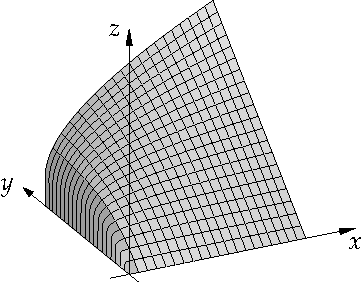
\includegraphics{figures/diffunderexample}
\caption{Grafik $z= \frac{x^y-1}{\ln(x)}$ pada $[0,1] \times [0,1]$.\label{fig:diffunderexample}}
\end{myfig}

Oleh karena itu,
$g$ adalah fungsi kontinu pada $[0,1]$, dan $g(0) = 0$.
Untuk $0 < \epsilon < 1$, turunan terhadap $y$ dari integran, yaitu $x^y$,
kontinu pada $[0,1] \times [\epsilon,1]$.  Oleh karena itu,
untuk $y >0$ kita boleh mendiferensialkan di bawah tanda integral
\begin{equation*}
g'(y) =
\int_0^{1} \frac{\ln(x) x^y}{\ln(x)} \,dx 
=
\int_0^{1} x^y \,dx =
\frac{1}{y+1} .
\end{equation*}
Kita mengetahui bahwa $g$ kontinu pada $[0,1]$, $g(0)=0$, dan
untuk $y \in (0,1)$, $g$ terdiferensialkan serta
$g'(y) = \frac{1}{y+1}$.  Jadi $g(1) = \int_0^1 g'(y)\,dy = \ln(2)$.
Dengan kata lain,
\begin{equation*}
\int_0^{1} \frac{x-1}{\ln(x)} \,dx  = \ln(2).
\end{equation*}
\end{example}

\begin{exbox}
\begin{exercise} \label{exercise:counterexamplediffunder}
Buktikan dua pernyataan yang dikemukakan dalam
\exampleref{example:counterexamplediffunder}:
\begin{exparts}
\item
Buktikan bahwa $\frac{x-1}{\ln(x)}$ dapat diperluas menjadi fungsi kontinu pada
$[0,1]$.  Artinya, terdapat fungsi kontinu pada $[0,1]$
yang sama dengan $\frac{x-1}{\ln(x)}$ pada $(0,1)$.
\item
Buktikan bahwa $\frac{x^y-1}{\ln(x)}$ dapat diperluas menjadi fungsi kontinu
pada $[0,1] \times [0,1]$.
\end{exparts}
\end{exercise}

\begin{exercise}
Misalkan $h \colon \R \to \R$ kontinu dan $g
\colon \R \to \R$ terdiferensialkan secara kontinu serta memiliki dukungan
kompak ($g$ bernilai nol di luar suatu interval kompak).  Definisikan
\begin{equation*}
f(x) = \int_{-\infty}^\infty h(y)g(x-y) \, dy  .
\end{equation*}
Tunjukkan bahwa $f$ terdiferensialkan.
\end{exercise}

\begin{exercise}
Misalkan $f \colon \R \to \R$ adalah fungsi yang terdiferensialkan tak berhingga kali (semua turunannya ada)
sedemikian sehingga $f(0) = 0$.
\begin{exparts}
\item
Tunjukkan bahwa terdapat fungsi $g \colon \R \to \R$ yang terdiferensialkan
tak berhingga kali sedemikian sehingga $f(x) = x\,g(x)$.
\item
Tunjukkan bahwa
jika $f'(0) \neq 0$, maka $g(0) \neq 0$.
\end{exparts}
Petunjuk: Pertama tuliskan
$f(x) = \int_0^x f'(s) \,ds$, kemudian tulis ulang integral tersebut agar batasnya
dari $0$ hingga $1$.
\end{exercise}

\begin{exercise}%[\neededexmark]
\label{exercise:severalvariableLeibniz}
Misalkan $U \subset \R^n$ terbuka dan andaikan
$f(x,y_1,y_2,\ldots,y_n)$ adalah fungsi kontinu
yang didefinisikan pada $[0,1] \times U \subset \R^{n+1}$.
Andaikan
$\frac{\partial f}{\partial y_1},
\frac{\partial f}{\partial y_2},\ldots,
\frac{\partial f}{\partial y_n}$
ada dan kontinu pada $[0,1] \times U$.
Buktikan bahwa $F \colon U \to \R$ yang didefinisikan oleh
\begin{equation*}
F(y_1,y_2,\ldots,y_n) =
\int_0^1
f(x,y_1,y_2,\ldots,y_n)
\, dx
\avoidbreak
\end{equation*}
terdiferensialkan secara kontinu (turunan-turunan parsialnya ada dan
kontinu).
\end{exercise}

\begin{exercise}
\pagebreak[2]
Kerjakan contoh tandingan berikut: Misalkan
\begin{equation*}
f(x,y) =
\begin{cases}
\frac{xy^3}{{(x^2+y^2)}^2} & \text{jika } x \neq 0 \text{ atau } y \neq 0,\\
0 & \text{jika } x=0 \text{ dan } y=0.
\end{cases}
\end{equation*}
\begin{exparts}
\item
Buktikan bahwa untuk setiap $y$ tetap, fungsi $x \mapsto f(x,y)$
terintegralkan Riemann pada $[0,1]$ dan
\begin{equation*}
g(y) = \int_0^1 f(x,y) \, dx = \frac{y}{2y^2+2} .
\end{equation*}
Dengan demikian, $g'(y)$ ada dan kita memperoleh fungsi kontinu
\begin{equation*}
g'(y) = \frac{1-y^2}{2{(y^2+1)}^2} .
\end{equation*}
\item
Buktikan bahwa $\frac{\partial f}{\partial y}$ ada untuk semua $x$ dan $y$, lalu
hitunglah turunannya.
\item
Tunjukkan bahwa untuk semua $y$
\begin{equation*}
\int_0^1 \frac{\partial f}{\partial y} (x,y) \, dx
\qquad
\text{ada, tetapi}
\qquad
g'(0) \neq \int_0^1 \frac{\partial f}{\partial y} (x,0) \, dx .
\end{equation*}
\end{exparts}
\end{exercise}

\begin{exercise}
Kerjakan contoh tandingan berikut: Misalkan
\begin{equation*}
f(x,y) =
\begin{cases}
x \,\sin \left(\frac{y}{x^2+y^2}\right) & \text{jika } (x,y) \neq (0,0),\\
0 & \text{jika } (x,y)=(0,0).
\end{cases}
\end{equation*}
\begin{exparts}
\item
Buktikan bahwa $f$ kontinu pada seluruh $\R^2$.
Dengan demikian, fungsi berikut terdefinisi dengan baik untuk setiap $y \in \R$:
\begin{equation*}
g(y) = \int_0^1 f(x,y) \, dx .
\end{equation*}
\item
Buktikan bahwa $\frac{\partial f}{\partial y}$ ada untuk semua $(x,y)$,
tetapi tidak kontinu di $(0,0)$.
\item
Tunjukkan bahwa $\int_0^1 \frac{\partial f}{\partial y}(x,0) \, dx$ tidak
ada, bahkan jika kita menggunakan integral tak wajar, yaitu
bahwa limit
$\lim\limits_{h \downarrow 0} \int_h^1 \frac{\partial f}{\partial y}(x,0) \, dx$
tidak ada.
\end{exparts}
Catatan: Silakan gunakan apa yang Anda ketahui tentang sinus dan kosinus dari kalkulus.
\pagebreak[2]
\end{exercise}

\begin{exercise} \label{exercise:strongerleibniz}
Perkuat aturan integral Leibniz dengan cara berikut.
Misalkan $f \colon (a,b) \times (c,d) \to \R$ adalah fungsi kontinu terbatas,
sedemikian sehingga $\frac{\partial f}{\partial y}$ ada untuk semua $(x,y) \in (a,b)
\times (c,d)$ serta kontinu dan terbatas.  Definisikan
\begin{equation*}
g(y) = \int_a^b f(x,y) \,dx .
\end{equation*}
Maka $g \colon (c,d) \to \R$ terdiferensialkan secara kontinu dan
\begin{equation*}
g'(y) = \int_a^b \frac{\partial f}{\partial y}(x,y) \,dx .
\end{equation*}
Petunjuk: Lihat juga \exerciseref{exercise:integralcontcontextra} dan
\thmref{thm:dersconverge}.
\end{exercise}
\end{exbox}

%%%%%%%%%%%%%%%%%%%%%%%%%%%%%%%%%%%%%%%%%%%%%%%%%%%%%%%%%%%%%%%%%%%%%%%%%%%%%%

\section{Turunan dalam beberapa variabel real} \label{sec:derinsv}

\subsection{Turunan}

Dalam pembahasan berikut, norma $\snorm{\cdot}$ dari suatu vektor dalam $\R^n$
adalah norma Euklides
\glsadd{not:euclidnorm}%
$\snorm{x} = \sqrt{x_1^2+\cdots+x_n^2}$.
Ketika diterapkan pada pemetaan linear (sebuah matriks), norma ini adalah
\glsadd{not:operatornorm}%
\emph{\myindex{norma operator}}:
\begin{equation*}
\snorm{A} \overset{\text{def}}{=} \sup_{\snorm{x} = 1} \snorm{Ax} .
\end{equation*}
Latihan berikut merangkum beberapa fakta penting tentang norma operator
bagi pembaca yang belum mengenal norma ini.

\begin{exbox}
\begin{exercise}
\begin{exparts} 
\item
Buktikan bahwa jika $A$ adalah pemetaan linear antara ruang vektor
berdimensi hingga, maka $\snorm{A} < \infty$.
\item
Buktikan bahwa jika $A$ adalah pemetaan linear ruang vektor, maka
$\snorm{Ax} \leq \snorm{A} \snorm{x}$.
\item
Carilah sebuah matriks eksplisit $2 \times 2$, yaitu $A$, dan sebuah vektor $x \in \R^2$
sedemikian sehingga $\snorm{Ax} < \snorm{A} \snorm{x}$.
\item
Jika $A$ adalah matriks $1 \times n$ atau $n \times 1$, maka norma operator
$\snorm{A}$ sama dengan norma Euklides dari entri-entri $A$.
\end{exparts} 
\end{exercise}
\end{exbox}

Turunan $f \colon \R \to \R$ di $x \in \R$
ada jika terdapat bilangan $a$ (turunan $f$ di $x$) sedemikian sehingga
\begin{equation*}
\lim_{h \to 0} \abs{\frac{f(x+h)-f(x)}{h} - a} =
\lim_{h \to 0} \frac{\sabs{f(x+h)-f(x) - ah}}{\sabs{h}}
= 0.
\end{equation*}
Perkalian dengan $a$ merupakan peta linear dalam satu dimensi:
$h \mapsto ah$.  Jadi turunannya merupakan peta linear.
Mari kita perluas gagasan ini ke lebih banyak variabel.

\begin{defn}
Misalkan $U \subset \R^n$ terbuka.  Kita mengatakan bahwa $f \colon U \to \R^m$
\emph{terdiferensialkan (secara real)\index{terdiferensialkan secara real}}
di $x \in U$ jika terdapat
pemetaan linear $A \colon \R^n \to \R^m$ sedemikian sehingga
\begin{equation*}
\lim_{\substack{h \to 0\\h\in \R^n}}
\frac{\snorm{f(x+h)-f(x) - Ah}}{\snorm{h}} = 0 .
\end{equation*}
Kita menulis $Df|_x = A$\glsadd{not:mvder} dan
mengatakan bahwa $A$ adalah \emph{turunan (real)\index{turunan real}} dari $f$ di $x$.
Jika $f$ terdiferensialkan (secara real) di
setiap $x \in U$, kita mengatakan bahwa $f$ \emph{terdiferensialkan (secara real)}.  Lihat
\figureref{fig:svder}.
\end{defn}

\begin{myfig}
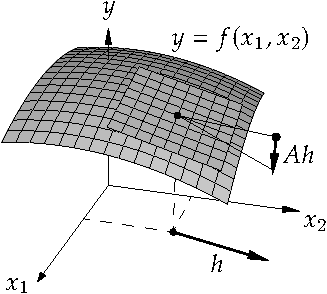
\includegraphics{figures/svder}
\caption{Ilustrasi turunan untuk fungsi $f \colon \R^2 \to \R$.  Vektor $h$ ditunjukkan
pada bidang $x_1x_2$ dengan pangkal di $(x_1,x_2)$, dan vektor
$Ah \in \R^1$ ditunjukkan sepanjang arah $y$.\label{fig:svder}}
\end{myfig}

Secara intuitif, $f$ terdiferensialkan di $x$ jika $f$ \myquote{sangat dekat secara infinitesimal}
dengan suatu peta linear di dekat $x$.
Kita tadi sedikit lancang dengan mengatakan bahwa $A$
adalah \emph{turunan tersebut}; mari kita buktikan bahwa pernyataan itu beralasan.

\begin{prop}
Misalkan $U \subset \R^n$ terbuka, $f \colon U \to \R^m$ suatu fungsi, dan
$x \in U$.
Andaikan $A,B \colon \R^n \to \R^m$ linear sedemikian sehingga
\begin{equation*}
\lim_{h \to 0}
\frac{\snorm{f(x+h)-f(x) - Ah}}{\snorm{h}} = 0
\qquad \text{dan} \qquad
\lim_{h \to 0}
\frac{\snorm{f(x+h)-f(x) - Bh}}{\snorm{h}} = 0 .
\end{equation*}
Maka $A=B$.
\end{prop}

\begin{proof}
Misalkan $h \in \R^n$, $h \neq 0$.  Hitunglah
\begin{equation*}
\begin{split}
\frac{\snorm{(A-B)h}}{\snorm{h}} & =
\frac{\snorm{-\bigl( f(x+h)-f(x) - Ah \bigr) + f(x+h)-f(x) - Bh}}{\snorm{h}} \\
& \leq
\frac{\snorm{f(x+h)-f(x) - Ah}}{\snorm{h}} + \frac{\snorm{f(x+h)-f(x) -
Bh}}{\snorm{h}} .
\end{split}
\end{equation*}
Jadi
$\frac{\snorm{(A-B)h}}{\snorm{h}} = \bnorm{(A-B)\frac{h}{\snorm{h}}} \to 0$
ketika $h \to 0$.  Setiap titik pada bola satuan dapat ditulis sebagai $\frac{h}{\snorm{h}}$
untuk $h$ yang sekecil apa pun, dan pemetaan linear yang lenyap pada bola satuan
bernilai nol di mana-mana.
\end{proof}

\begin{example}
Jika $f(x) = Ax$ untuk suatu pemetaan linear $A$, maka
$Df|_x = A$:
\begin{equation*}
\frac{\snorm{f(x+h)-f(x) - Ah}}{\snorm{h}}
=
\frac{\snorm{A(x+h)-Ax - Ah}}{\snorm{h}}
=
\frac{0}{\snorm{h}} = 0 .
\end{equation*}
\end{example}

\begin{example}
Misalkan $f \colon \R^2 \to \R^2$ didefinisikan oleh
\begin{equation*}
f(x,y) = \bigl(f_1(x,y),f_2(x,y)\bigr) = (1+x+2y+x^2,2x+3y+xy).
\end{equation*}
Mari kita tunjukkan bahwa $f$ terdiferensialkan di titik asal dan
menghitung turunannya,
langsung dengan menggunakan definisi.  Jika
turunannya ada, turunan tersebut dapat
direpresentasikan oleh matriks berukuran $2$-kali-$2$
$\left[\begin{smallmatrix}a&b\\c&d\end{smallmatrix}\right]$.  Misalkan $h =
(h_1,h_2)$.  Kita memerlukan agar ekspresi berikut menuju nol.
\begin{multline*}
\frac{\snorm{
f(h_1,h_2)-f(0,0)
-
(ah_1 +bh_2 , ch_1+dh_2)}
}{\snorm{(h_1,h_2)}}
=
\\
\frac{\sqrt{
{\bigl((1-a)h_1 + (2-b)h_2 + h_1^2\bigr)}^2
+
{\bigl((2-c)h_1 + (3-d)h_2 + h_1h_2\bigr)}^2}}{\sqrt{h_1^2+h_2^2}} .
\end{multline*}
Jika kita memilih $a=1$, $b=2$, $c=2$, $d=3$, ekspresi tersebut menjadi
\begin{equation*}
\frac{\sqrt{
h_1^4 + h_1^2h_2^2}}{\sqrt{h_1^2+h_2^2}}
=
\sabs{h_1}
\frac{\sqrt{
h_1^2 + h_2^2}}{\sqrt{h_1^2+h_2^2}}
= \sabs{h_1} .
\end{equation*}
Dan ekspresi ini memang menuju nol ketika $h \to 0$.  Fungsi
$f$ terdiferensialkan di titik asal dan
turunan $Df|_0$ direpresentasikan oleh matriks
$\left[\begin{smallmatrix}1&2\\2&3\end{smallmatrix}\right]$.
\end{example}

\begin{prop}
Misalkan $U \subset \R^n$ terbuka dan $f \colon U \to \R^m$
terdiferensialkan di $p \in U$.  Maka $f$ kontinu di $p$.
\end{prop}

\begin{proof}
Cara lain untuk menuliskan keterdiferensialan $f$ di $p$ adalah dengan mempertimbangkan
\begin{equation*}
r(h) = f(p+h)-f(p) - Df|_p h .
\end{equation*}
Fungsi $f$ terdiferensialkan di $p$ jika
$\frac{\snorm{r(h)}}{\snorm{h}}$ menuju nol ketika $h \to 0$,
sehingga
$r(h)$ menuju nol.  Turunan $D f|_p$
adalah peta linear dari $\R^n$ ke $\R^m$ dan karena itu
$D f|_p h \to 0$ ketika $h \to 0$.  Jadi,
$f(p+h)$ menuju $f(p)$ ketika $h \to 0$.
\end{proof}

Turunan itu sendiri merupakan operator linear pada ruang fungsi-fungsi
yang terdiferensialkan.

\begin{prop}
Andaikan $U \subset \R^n$ terbuka,
$f \colon U \to \R^m$ dan
$g \colon U \to \R^m$ terdiferensialkan di $p$,
dan $\alpha \in \R$.  Maka fungsi $f+g$ dan $\alpha f$
terdiferensialkan di $p$, dan
\begin{equation*}
D(f+g)|_p = Df|_p + Dg|_p \qquad \text{dan} \qquad D(\alpha f)|_p = \alpha
Df|_p .
\end{equation*}
\end{prop}

\begin{proof}
Misalkan $h \in \R^n$, $h \neq 0$.  Proposisi ini mengikuti dari taksiran-taksiran
berikut:
\begin{multline*}
\frac{\norm{f(p+h)+g(p+h)-\bigl(f(p)+g(p)\bigr) - \bigl(Df|_p + Dg|_p\bigr)h}}{\snorm{h}}
\\
\leq
\frac{\norm{f(p+h)-f(p) - Df|_ph}}{\snorm{h}}
+
\frac{\norm{g(p+h)-g(p) - Dg|_ph}}{\snorm{h}} ,
\end{multline*}
dan
\begin{equation*}
\frac{\norm{\alpha f(p+h) - \alpha f(p) - \alpha Df|_p h}}{\snorm{h}}
=
\sabs{\alpha} \frac{\norm{f(p+h))-f(p) - Df|_ph}}{\snorm{h}} .
\qedhere
\end{equation*}
\end{proof}

Jika $A \colon \R^n \to \R^m$ dan $B \colon \R^m \to \R^k$ linear, maka
keduanya merupakan turunannya sendiri.  Komposisi
$BA$, suatu peta linear dari $\R^n$ ke $\R^k$, juga merupakan turunannya sendiri, sehingga
turunan suatu komposisi adalah komposisi
dari turunan-turunannya.
Karena peta-peta yang terdiferensialkan \myquote{sangat dekat secara infinitesimal}
dengan peta linear, peta-peta tersebut memiliki sifat yang sama:

\begin{thm}[Aturan rantai]\index{aturan rantai!turunan real} \label{thm:realchain}
Misalkan $U \subset \R^n$ terbuka dan $f \colon U \to \R^m$
terdiferensialkan di $p \in U$.  Misalkan $V \subset \R^m$ terbuka,
$f(U) \subset V$, dan $g \colon V \to \R^\ell$ terdiferensialkan
di $f(p)$.  Maka
\begin{equation*}
F(x) = g\bigl(f(x)\bigr)
\end{equation*}
terdiferensialkan di $p$ dan
\begin{equation*}
DF|_p = Dg|_{f(p)} Df|_p .
\end{equation*}
\end{thm}

\begin{proof}
Misalkan $A = Df|_p$ dan $B = Dg|_{f(p)}$.  Ambil $h \in \R^n$ tak nol,
tulis $q = f(p)$, $k = f(p+h)-f(p)$, dan misalkan
\begin{equation*}
r(h) = f(p+h)-f(p) - A h .
\end{equation*}
Maka $r(h) = k-Ah$ atau $Ah = k-r(h)$, dan $f(p+h) = q+k$.
Selanjutnya
\begin{equation*}
\begin{split}
\frac{\snorm{F(p+h)-F(p) - BAh}}{\snorm{h}}
& =
\frac{\bnorm{g\bigl(f(p+h)\bigr)-g\bigl(f(p)\bigr) - BAh}}{\snorm{h}}
\\
& =
\frac{\bnorm{g(q+k)-g(q) - B\bigl(k-r(h)\bigr)}}{\snorm{h}}
\\
& \leq
\frac
{\snorm{g(q+k)-g(q) - Bk}}
{\snorm{h}}
+
\snorm{B}
\frac
{\snorm{r(h)}}
{\snorm{h}}
\end{split}
\end{equation*}
Pertama, $\snorm{B}$ konstan dan $f$ terdiferensialkan di $p$,
sehingga
$\snorm{B}\frac{\snorm{r(h)}}{\snorm{h}} \to 0$
ketika $h \to 0$.
Selanjutnya,
jika $k=0$, maka $\frac
{\snorm{g(q+k)-g(q) - Bk}}
{\snorm{h}} = 0$, jadi andaikan $k \neq 0$.  Kita memperoleh
\begin{equation*}
\frac
{\snorm{g(q+k)-g(q) - Bk}}
{\snorm{h}}
=
\frac
{\snorm{g(q+k)-g(q) - Bk}}
{\snorm{k}}
\frac
{\snorm{f(p+h)-f(p)}}
{\snorm{h}} .
\end{equation*}
Karena $f$ kontinu di $p$, kita memperoleh bahwa
$k \to 0$ ketika
$h \to 0$.
Oleh karena itu,
$\frac
{\snorm{g(q+k)-g(q) - Bk}}
{\snorm{k}} \to 0$ karena $g$ terdiferensialkan di $q$.
Terakhir,
\begin{equation*}
\frac
{\snorm{f(p+h)-f(p)}}
{\snorm{h}}
\leq
\frac
{\snorm{f(p+h)-f(p)-Ah}}
{\snorm{h}}
+
\snorm{A} .
\end{equation*}
Karena $f$ terdiferensialkan di $p$,
ruas kanan tetap terbatas ketika $h \to 0$.
%Oleh karena itu,
%$
%\frac
%{\snorm{f(p+h)-f(p)}}
%{\snorm{h}}
%$
%tetap terbatas ketika $h \to 0$,
Jadi
$\frac
{\snorm{g(q+k)-g(q) - Bk}}
{\snorm{h}} \to 0$ ketika $h \to 0$.
Dengan demikian,
$\frac{\snorm{F(p+h)-F(p) - BAh}}{\snorm{h}} \to 0$, dan
$DF|_p = BA$.
\end{proof}

Mari kita buktikan sebuah \myquote{teorema nilai rata-rata} untuk fungsi bernilai vektor.
Untuk fungsi $\varphi \colon [a,b] \to \R^n$, kita memandang turunan
$D\varphi|_{t_0}$ sebagai vektor dalam $\R^n$, dan sebagai
sebuah vektor kita akan menuliskannya sebagai
$\varphi'(t_0)$.
Tidak sulit untuk memeriksa bahwa
entri-entri matriks $D\varphi|_{t_0}$
(sebuah peta linear dari $\R$ ke $\R^n$)
hanyalah turunan dari
komponen-komponen $\varphi$,
dan $D\varphi|_{t_0} h = h \varphi'(t_0)$.  Selanjutnya
$\snorm{\varphi'(t_0)}$
adalah norma Euklides dalam $\R^n$.  Bahkan, dalam konteks ini norma tersebut sama
dengan norma operator $D\varphi|_{t_0}$.

\begin{lemma}
Jika $\varphi \colon [a,b] \to \R^n$ terdiferensialkan pada $(a,b)$ dan
kontinu pada $[a,b]$, maka terdapat $t_0 \in (a,b)$ sedemikian sehingga
\begin{equation*}
\snorm{\varphi(b)-\varphi(a)} \leq (b-a) \snorm{\varphi'(t_0)} .
\end{equation*}
\end{lemma}

\begin{proof}
Menurut teorema nilai rata-rata pada fungsi bernilai skalar
$t \mapsto \bigl(\varphi(b)-\varphi(a) \bigr) \cdot \varphi(t)$,
dengan titik menyatakan hasil kali titik, kita memperoleh
bahwa
terdapat $t_0 \in (a,b)$ sedemikian sehingga
\begin{equation*}
\begin{split}
\snorm{\varphi(b)-\varphi(a)}^2
& =
\bigl( \varphi(b)-\varphi(a) \bigr)
\cdot
\bigl( \varphi(b)-\varphi(a) \bigr)
\\
& =
\bigl(\varphi(b)-\varphi(a) \bigr) \cdot \varphi(b) - 
\bigl(\varphi(b)-\varphi(a) \bigr) \cdot \varphi(a)
\\
& = 
(b-a)
\bigl(\varphi(b)-\varphi(a) \bigr) \cdot \varphi'(t_0) .
\end{split}
\end{equation*}
Menurut ketaksamaan Cauchy--Schwarz,
\begin{equation*}
\snorm{\varphi(b)-\varphi(a)}^2
=
(b-a)\bigl(\varphi(b)-\varphi(a) \bigr) \cdot \varphi'(t_0)
\leq
(b-a)
\snorm{\varphi(b)-\varphi(a)} \, \snorm{\varphi'(t_0)} . \qedhere
\end{equation*}
\end{proof}

Ingat bahwa suatu himpunan $U$ disebut konveks
jika untuk setiap $x,y \in U$, ruas garis dari
$x$ ke $y$ terletak di dalam $U$.

\begin{prop} \label{mv:prop:convexlip}
Misalkan $U \subset \R^n$ adalah himpunan terbuka konveks, $f \colon U \to \R^m$
suatu fungsi terdiferensialkan, dan $M$ sedemikian sehingga
\begin{equation*}
\snorm{Df|_x} \leq M
\qquad \text{untuk semua } x \in U.
\end{equation*}
Maka $f$ bersifat Lipschitz dengan konstanta $M$, yaitu
\begin{equation*}
\snorm{f(x)-f(y)} \leq M \snorm{x-y}
\qquad
\text{untuk semua } x,y \in U.
\end{equation*}
\end{prop}

\begin{proof}
Tetapkan $x,y \in U$.  Karena sifat konveks,
$(1-t)x+ty \in U$ untuk semua $t \in [0,1]$.
Selanjutnya
\begin{equation*}
\frac{d}{dt} \Bigl[f\bigl((1-t)x+ty\bigr)\Bigr]
=
Df|_{((1-t)x+ty)} (y-x) .
\end{equation*}
Menurut teorema nilai rata-rata di atas, untuk
suatu $t_0 \in (0,1)$,
\begin{equation*}
\begin{split}
\snorm{f(x)-f(y)} & \leq
\norm{\frac{d}{dt} \Big|_{t=t_0} \Bigl[ f\bigl((1-t)x+ty\bigr) \Bigr] }
\\
& \leq
\norm{Df|_{((1-t_0)x+t_0y)}} \, \snorm{y-x} \leq
M \snorm{y-x} . \qedhere
\end{split}
\end{equation*}
\end{proof}

Mari kita selesaikan persamaan diferensial $Df = 0$.

\begin{cor} \label{thm:svzerodersol}
Jika $U \subset \R^n$ terbuka dan terhubung, $f \colon U \to \R^m$ terdiferensialkan,
dan $Df|_x = 0$ untuk semua $x \in U$, maka $f$ konstan.
\end{cor}

\begin{proof}
Untuk setiap $x \in U$, terdapat bola terbuka $B(x,\delta) \subset U$.  Bola
$B(x,\delta)$ bersifat konveks.  Karena
$\snorm{Df|_y} \leq 0$ untuk semua $y \in B(x,\delta)$, kita memperoleh
$\snorm{f(x)-f(y)} \leq 0 \snorm{x-y} = 0$.
Dengan demikian, $f^{-1}(c)$ terbuka untuk setiap $c \in \R^m$.  Andaikan
$f^{-1}(c)$ tak kosong.
Kedua himpunan
\begin{equation*}
U' = f^{-1}(c), \qquad U'' = f^{-1}\bigl(\R^m\setminus\{c\}\bigr)
\end{equation*}
terbuka dan saling lepas, dan lebih lanjut $U = U' \cup U''$.  Karena $U'$ tak kosong
dan $U$ terhubung, $U'' = \emptyset$.  Jadi $f(x) = c$ untuk semua $x \in U$.
\end{proof}

\begin{exbox}
\begin{exercise}
Dengan hanya menggunakan definisi turunan, tunjukkan bahwa
fungsi-fungsi $f \colon \R^2 \to \R^2$ berikut terdiferensialkan di titik asal dan
carilah turunannya.
\begin{exparts}
\item
$f(x,y) = (1+x+xy,x)$,
\item
$f(x,y) = \bigl(y-y^{10},x \bigr)$,
\item
$f(x,y) = \bigl( {(x+y+1)}^2 , {(x-y+2)}^2 \bigr)$.
\end{exparts}
\end{exercise}

\begin{exercise}
Definisikan $f \colon \R^2 \to \R^2$ dengan $f(x,y) =
\bigl(x,y+\varphi(x)\bigr)$ untuk suatu fungsi satu variabel $\varphi$ yang
terdiferensialkan.  Tunjukkan bahwa $f$ terdiferensialkan dan carilah $Df$.
\end{exercise}

\begin{exercise}
Andaikan $f \colon \R^n \to \R$ dan $h \colon \R^n \to \R$
terdiferensialkan dan $Df|_x = Dh|_x$ untuk semua $x \in \R^n$.
Buktikan bahwa
jika $f(0) = h(0)$, maka $f(x) = h(x)$ untuk semua $x \in \R^n$.
\end{exercise}
\end{exbox}


\subsection{Turunan dalam suku-suku turunan parsial}

Turunan parsial lebih mudah dihitung dengan seluruh perangkat
kalkulus, dan turunan tersebut menyediakan cara untuk menghitung turunan suatu
fungsi.

\begin{prop} \label{mv:prop:jacobianmatrix}
Misalkan $U \subset \R^n$ terbuka dan $f \colon U \to \R^m$
terdiferensialkan di $p \in U$.  Maka semua turunan parsial di $p$
ada dan, dalam basis standar $\R^n$ dan $\R^m$,
$Df|_p$ direpresentasikan oleh matriks
\begin{equation*}
\begin{bmatrix}
\frac{\partial f_1}{\partial x_1}\big|_p
&
\frac{\partial f_1}{\partial x_2}\big|_p
& \ldots &
\frac{\partial f_1}{\partial x_n}\big|_p
\\[6pt]
\frac{\partial f_2}{\partial x_1}\big|_p
&
\frac{\partial f_2}{\partial x_2}\big|_p
& \ldots &
\frac{\partial f_2}{\partial x_n}\big|_p
\\
\vdots & \vdots & \ddots & \vdots
\\
\frac{\partial f_m}{\partial x_1}\big|_p
&
\frac{\partial f_m}{\partial x_2}\big|_p
& \ldots &
\frac{\partial f_m}{\partial x_n}\big|_p
\end{bmatrix} .
\end{equation*}
\end{prop}

Dengan kata lain,
\begin{equation*}
Df|_p \, e_j =
\sum_{k=1}^m
\frac{\partial f_k}{\partial x_j}\Big|_p \,e_k ,
\end{equation*}
dengan $e_j$ menyatakan vektor-vektor basis standar dalam ruang yang sesuai.
Ingat bahwa unsur basis standar $e_j$ adalah vektor yang semua entrinya nol
kecuali sebuah $1$ pada entri ke-$j$\textsuperscript{}.

\begin{proof}
Tetapkan suatu $j$ dan perhatikan bahwa untuk $h$ tak nol,
\begin{equation*}
\begin{split}
\norm{\frac{f(p+h e_j)-f(p)}{h} - Df|_p \, e_j} & = 
\norm{\frac{f(p+h e_j)-f(p) - Df|_p \, h e_j}{h}} \\
& =
\frac{\snorm{f(p+h e_j)-f(p) - Df|_p \, h e_j}}{\snorm{h e_j}} .
\end{split}
\end{equation*}
Ketika $h$ menuju $0$, ruas kanan menuju nol karena
keterdiferensialan $f$, dan karena itu
\begin{equation*}
\lim_{h \to 0}
\frac{f(p+h e_j)-f(p)}{h} = Df|_p \, e_j  .
\end{equation*}
Mari kita representasikan $f$ melalui komponen-komponennya,
$f = (f_1,f_2,\ldots,f_m)$, karena fungsi tersebut bernilai vektor.
Mengambil limit dalam $\R^m$
sama dengan mengambil limit dalam setiap komponennya secara terpisah.
Untuk setiap $k$,
\begin{equation*}
\frac{\partial f_k}{\partial x_j} \Big|_p
=
\lim_{h \to 0}
\frac{f_k(p+h e_j)-f_k(p)}{h}
\end{equation*}
ada dan
sama dengan komponen ke-$k$\textsuperscript{} dari $Df|_p\, e_j$, sehingga pembuktian selesai.
\end{proof}

Kebalikan proposisi tersebut tidak benar.  Adanya turunan-turunan parsial
tidak berarti bahwa fungsinya terdiferensialkan.
Namun, ketika turunan-turunan parsial tersebut kontinu,
pernyataan kebalikannya berlaku.


\begin{defn}
Misalkan $U \subset \R^n$ terbuka.
Kita mengatakan bahwa $f \colon U \to \R^m$
\emph{\myindex{terdiferensialkan secara kontinu}},
jika semua turunan parsial
$\frac{\partial f_j}{\partial x_k}$ ada dan kontinu.\footnote{%
Sebagai alternatif, orang mendefinisikan bahwa $f$ terdiferensialkan secara kontinu
jika $Df|_x$ merupakan fungsi kontinu yang memetakan $x \in U$ ke ruang operator
linear.  Proposisi-proposisi dalam bagian ini menyatakan bahwa kedua definisi tersebut ekuivalen.}
\end{defn}

\begin{prop} \label{mv:prop:contdiffpartials}
Misalkan $U \subset \R^n$ terbuka.
Jika $f \colon U \to \R^m$
terdiferensialkan secara kontinu, maka
$f$ terdiferensialkan.
\end{prop}

\begin{proof}
Tetapkan $p \in U$.  Kita melakukan induksi pada dimensi.  Kasus $n=1$ diserahkan
sebagai latihan.
Andaikan kesimpulan tersebut benar untuk $\R^{n-1}$,
yaitu,
jika kita membatasi pada $n-1$ variabel pertama, fungsi tersebut terdiferensialkan.
Turunan parsial $n-1$ pertama dari $f$ yang dibatasi pada himpunan tempat koordinat terakhir
ditetapkan sama dengan turunan parsial untuk $f$.
Dalam pembahasan berikut, dengan sedikit penyalahgunaan notasi,
kita memandang $\R^{n-1}$ sebagai himpunan bagian dari $\R^n$, yaitu himpunan dalam $\R^n$ tempat $x_n = 0$.
Dengan kata lain, kita mengidentifikasi vektor $(x_1,x_2,\ldots,x_{n-1})$ dan
$(x_1,x_2,\ldots,x_{n-1},0)$.
Misalkan
\begin{equation*}
A = 
\begin{bmatrix}
\frac{\partial f_1}{\partial x_1}\big|_p
& \ldots &
\frac{\partial f_1}{\partial x_n}\big|_p
\\
\vdots & \ddots & \vdots
\\
\frac{\partial f_m}{\partial x_1}\big|_p
& \ldots &
\frac{\partial f_m}{\partial x_n}\big|_p
\end{bmatrix} ,
\qquad
A' = 
\begin{bmatrix}
\frac{\partial f_1}{\partial x_1}\big|_p
& \ldots &
\frac{\partial f_1}{\partial x_{n-1}}\big|_p
\\
\vdots & \ddots & \vdots
\\
\frac{\partial f_m}{\partial x_1}\big|_p
& \ldots &
\frac{\partial f_m}{\partial x_{n-1}}\big|_p
\end{bmatrix} ,
\qquad
v = 
\begin{bmatrix}
\frac{\partial f_1}{\partial x_n}\big|_p
\\
\vdots
\\
\frac{\partial f_m}{\partial x_n}\big|_p
\end{bmatrix} .
\end{equation*}
Misalkan $\epsilon > 0$ diberikan.  Menurut hipotesis induksi, terdapat
$\delta > 0$ sedemikian sehingga
untuk setiap $h' \in \R^{n-1}$ dengan $\snorm{h'} < \delta$,
\begin{equation*}
\frac{\snorm{f(p+h') - f(p) - A' h'}}{\snorm{h'}} < \epsilon .
\end{equation*}
Berdasarkan kekontinuan turunan-turunan parsial, andaikan $\delta$ cukup
kecil sehingga
\begin{equation*}
\abs{\frac{\partial f_k}{\partial x_n}\Big|_{p+h}
      - \frac{\partial f_k}{\partial x_n}\Big|_{p}} < \epsilon ,
\end{equation*}
untuk semua $k$ dan semua $h \in \R^n$ dengan $\snorm{h} < \delta$.

Andaikan $h = h' + t e_n$ adalah vektor dalam $\R^n$, dengan $h' \in \R^{n-1}$,
$t \in \R$, sedemikian sehingga
$\snorm{h} < \delta$.  Maka $\snorm{h'} \leq \snorm{h} < \delta$.
Perhatikan bahwa $Ah = A' h' + tv$.
\begin{equation*}
\begin{split}
\snorm{f(p+h) - f(p) - Ah}
& = \snorm{f(p+h' + t e_n) - f(p+h') - tv + f(p+h') - f(p) - A' h'}
\\
& \leq \snorm{f(p+h' + t e_n) - f(p+h') -tv} + \snorm{f(p+h') - f(p) -
A' h'}
\\
& \leq \snorm{f(p+h' + t e_n) - f(p+h') -tv} + \epsilon \snorm{h'} .
\end{split}
\end{equation*}
Karena semua turunan parsial ada, menurut teorema nilai rata-rata,
untuk setiap $k$ terdapat $\theta_k$, dengan $\sabs{\theta_k} \leq \sabs{t}$, sedemikian sehingga
\begin{equation*}
f_k(p+h' + t e_n) - f_k(p+h') =
t \frac{\partial f_k}{\partial x_n}\Big|_{(p+h'+\theta_k e_n)}.
\end{equation*}
Perhatikan bahwa $\snorm{h'+\theta_k e_n} \leq \snorm{h} < \delta$.
Untuk menyelesaikan pembuktian,
\begin{equation*}
\begin{split}
\snorm{f(p+h) - f(p) - Ah}
& \leq \snorm{f(p+h' + t e_n) - f(p+h') -tv} + \epsilon \snorm{h'}
\\
& \leq \sqrt{\sum_{k=1}^m
{\left(t\frac{\partial f_k}{\partial x_n}\Big|_{(p+h'+\theta_k e_n)} -
t \frac{\partial f_k}{\partial x_n}\Big|_{p}\right)}^2} + \epsilon \snorm{h'}
\\
& \leq \sqrt{m}\, \epsilon \sabs{t} + \epsilon \snorm{h'}
\\
& \leq (\sqrt{m}+1)\epsilon \snorm{h} . \qedhere
\end{split}
\end{equation*}
\end{proof}

\begin{exbox}
\begin{exercise}
Buktikan kasus dasar
dalam \propref{mv:prop:contdiffpartials}:
Jika $n=1$ dan
\myquote{turunan-turunan parsialnya ada dan kontinu,} maka fungsi tersebut
terdiferensialkan.  Perhatikan bahwa $f$ bernilai vektor.
\end{exercise}

\begin{exercise}
Definisikan fungsi $f \colon \R^2 \to \R$ dengan
(lihat \figureref{fig:xyxsqysqvol2})
\begin{equation*}
f(x,y)
=
\begin{cases}
\frac{xy}{x^2+y^2} & \text{jika } (x,y) \neq (0,0), \\
0 & \text{jika } (x,y) = (0,0).
\end{cases}
\end{equation*}
\begin{exparts}
\item
Tunjukkan bahwa turunan parsial
$\frac{\partial f}{\partial x}$ dan
$\frac{\partial f}{\partial y}$ ada di semua titik (termasuk titik asal).
\item
Tunjukkan bahwa $f$ tidak kontinu di titik asal (dan karena itu tidak
terdiferensialkan).
\item
Tunjukkan bahwa turunan-turunan parsial tersebut tidak kontinu.
\end{exparts}
\end{exercise}

\begin{exercise}
Definisikan $f \colon \R^2 \to \R$ sebagai
\begin{equation*}
f(x,y) =
\begin{cases}
(x^2+y^2)\sin\bigl({(x^2+y^2)}^{-1}\bigr) & \text{jika } (x,y) \neq (0,0), \\
0 & \text{jika } (x,y) = (0,0).
\end{cases}
\end{equation*}
Tunjukkan bahwa $f$ terdiferensialkan di titik asal, tetapi tidak
terdiferensialkan secara kontinu.
\end{exercise}
\end{exbox}

\begin{myfig}
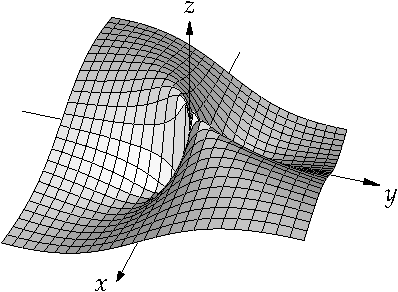
\includegraphics{figures/xyxsqysq}
\caption{Grafik $\frac{xy}{x^2+y^2}$.\label{fig:xyxsqysqvol2}}
\end{myfig}

\subsection{Teorema titik tetap}

Sebelum membuktikan teorema fungsi invers, kita harus mengambil jalan memutar untuk membuktikan
sebuah teorema titik tetap bagi ruang metrik.

\begin{defn}
Misalkan $(X,d_X)$ dan $(Y,d_Y)$ adalah ruang metrik.
Suatu pemetaan
$f \colon X \to Y$ disebut \emph{\myindex{kontraksi}}
(atau peta kontraktif) jika merupakan
peta $k$-Lipschitz untuk suatu $k < 1$, yaitu jika terdapat $k < 1$ sedemikian sehingga
\begin{equation*}
d_Y\bigl(f(p),f(q)\bigr) \leq k\, d_X(p,q)
\qquad \text{untuk semua } p,q \in X.
\avoidbreak
\end{equation*}
Jika $f \colon X \to X$ adalah sebuah peta, $x \in X$ disebut
\emph{\myindex{titik tetap}}
jika $f(x)=x$.
\end{defn}

\begin{thm}%
[Prinsip pemetaan kontraksi\index{prinsip pemetaan kontraksi}
atau \myindex{teorema titik tetap Banach}\index{teorema titik tetap}]
\label{thm:contr}
Misalkan $(X,d)$ adalah ruang metrik lengkap tak kosong dan $f \colon X \to X$ suatu
kontraksi.
Maka $f$ memiliki tepat satu titik tetap.
\end{thm}

\begin{proof}
Pilih sembarang $x_0 \in X$.
Definisikan barisan $\{ x_n \}$ dengan $x_{n+1} = f(x_n)$.
\begin{equation*}
d(x_{n+1},x_n) = d\bigl(f(x_n),f(x_{n-1})\bigr)
\leq k d(x_n,x_{n-1})
\leq \cdots
\leq k^n d(x_1,x_0) .
\end{equation*}
Andaikan $m > n$, maka
\begin{multline*}
d(x_m,x_n)
\leq \sum_{\ell=n}^{m-1} d(x_{\ell+1},x_\ell)
\leq \sum_{\ell=n}^{m-1} k^\ell d(x_1,x_0)
= k^n d(x_1,x_0) \sum_{\ell=0}^{m-n-1} k^\ell
\\
\leq k^n d(x_1,x_0) \sum_{\ell=0}^{\infty} k^\ell
= k^n d(x_1,x_0) \frac{1}{1-k} .
\end{multline*}
Jadi barisan tersebut adalah barisan Cauchy.  Karena $X$ lengkap,
misalkan $x = \lim\, x_n$.  Kita mengklaim bahwa $x$
adalah titik tetap tunggal yang dicari.

Titik tetap?  Fungsi $f$ merupakan kontraksi,
sehingga kontinu Lipschitz:
\begin{equation*}
f(x) = f( \lim \, x_n) = \lim\, f(x_n) = \lim\, x_{n+1} = x .
\end{equation*}

Tunggal?  Misalkan $x$ dan $y$ keduanya merupakan titik tetap.
\begin{equation*}
d(x,y) = d\bigl(f(x),f(y)\bigr) \leq k\, d(x,y) .
\end{equation*}
Karena $k < 1$, kita memperoleh $d(x,y) = 0$ dan karena itu $x=y$.  Teorema
telah terbukti.
\end{proof}

Pembuktiannya bersifat konstruktif.  Kita bukan hanya mengetahui
bahwa terdapat tepat satu titik tetap, tetapi juga mengetahui cara menemukannya.  Mulailah dengan
sembarang $x_0 \in X$ dan iterasikan $f(x_0)$,
$f(f(x_0))$,
$f(f(f(x_0)))$, dan seterusnya.

\begin{exbox}
\begin{exercise}
\begin{exparts}
\item
Carilah contoh kontraksi $f \colon X \to X$
pada ruang metrik tak lengkap $X$ yang tidak memiliki
titik tetap.
\item
Carilah peta $1$-Lipschitz $f \colon X \to X$ pada ruang metrik lengkap $X$ yang tidak memiliki titik tetap.
\end{exparts}
\end{exercise}

\begin{exercise}
Misalkan $f(x) = x-\frac{x^2-2}{2x}$ (Anda mungkin mengenalinya sebagai metode Newton untuk
$\sqrt{2}$).
\begin{exparts}
\item
Buktikan bahwa $f\bigl([1,\infty)\bigr) \subset [1,\infty)$.
\item
Buktikan bahwa $f \colon [1,\infty) \to [1,\infty)$ merupakan kontraksi.
\item
Terapkan teorema titik tetap untuk menemukan $x \geq 1$ sedemikian sehingga
$f(x) = x$, dan tunjukkan bahwa $x = \sqrt{2}$.
\end{exparts}
\end{exercise}
\end{exbox}

\subsection{Teorema fungsi invers}
\label{subsec:svinvfuncthm}

Secara intuitif, kita kembali beranggapan bahwa jika suatu fungsi terdiferensialkan secara kontinu, maka fungsi tersebut
secara lokal \myquote{berperilaku seperti} turunannya (suatu fungsi linear).
Gagasan teorema fungsi invers adalah bahwa jika suatu fungsi
terdiferensialkan secara kontinu dan turunannya dapat dibalik, maka fungsi tersebut
dapat dibalik (secara lokal).
%Untuk membuktikan teorema ini, kita menggunakan prinsip pemetaan
%kontraksi (\thmref{thm:contr}).

\begin{thm}[Teorema fungsi invers]\index{teorema fungsi invers!versi real}
\label{thm:inverse}
Andaikan $U \subset \R^n$ terbuka,
$f \colon U \to \R^n$ terdiferensialkan secara kontinu, $p \in U$, dan $Df|_p$ dapat dibalik
(yaitu, $\det Df|_p \neq 0$).
Maka terdapat himpunan terbuka $V, W \subset \R^n$ sedemikian sehingga
$p \in V \subset U$, $f(V) = W$, pembatasan $f|_V$ bersifat injektif (satu-ke-satu),
dan karena itu terdapat $g \colon W \to V$ sedemikian sehingga
$g(y) = (f|_V)^{-1}(y)$ untuk semua $y \in W$.
Lihat \figureref{fig:inversefuncRn}.
Lebih lanjut, $g$ terdiferensialkan secara kontinu
dan
\begin{equation*}
Dg|_y = {\bigl(Df|_x\bigr)}^{-1}, \qquad \text{untuk semua } x \in V, y = f(x).
\end{equation*}
\end{thm}

\begin{myfig}
\subimport*{figures/}{inversefuncRn.pdf_t}
\caption{Susunan teorema fungsi invers dalam $\R^n$.\label{fig:inversefuncRn}}
\end{myfig}

\begin{proof}
Tuliskan $A = Df|_p$.  Karena $Df$ kontinu, terdapat bola terbuka
$V$ di sekitar $p$ sedemikian sehingga
\begin{equation*}
\snorm{A-Df|_x} < \frac{1}{2\snorm{A^{-1}}}
\qquad \text{untuk semua } x \in V.
\avoidbreak
\end{equation*}
Ketaksamaan tersebut mengakibatkan bahwa $Df|_x$ dapat dibalik untuk semua $x \in V$
(lihat latihan di bawah).

Untuk suatu $y \in \R^n$, definisikan $\varphi_y \colon C \to \R^n$ dengan
\begin{equation*}
\varphi_y (x) = x + A^{-1}\bigl(y-f(x)\bigr) .
\end{equation*}
Karena $A^{-1}$ bersifat satu-ke-satu,
$\varphi_y(x) = x$ ($x$ adalah titik tetap) jika dan hanya jika
$y-f(x) = 0$, atau dengan kata lain $f(x)=y$.  Dengan menggunakan aturan rantai, kita memperoleh
\begin{equation*}
D\varphi_y|_x = I - A^{-1} Df|_x = A^{-1} \bigl( A-Df|_x \bigr) .
\end{equation*}
Jadi untuk $x \in V$,
\begin{equation*}
\snorm{D\varphi_y|_x} \leq \snorm{A^{-1}} \, \snorm{A-Df|_x} < \nicefrac{1}{2} .
\end{equation*}
Karena $V$ adalah bola, bola tersebut bersifat konveks.  Oleh karena itu,
\begin{equation*}
\snorm{\varphi_y(x_1)-\varphi_y(x_2)} \leq \frac{1}{2} \snorm{x_1-x_2} 
\qquad
\text{untuk semua } x_1,x_2 \in V.
\end{equation*}
Dengan kata lain, $\varphi_y$ adalah kontraksi yang didefinisikan pada $V$, meskipun sejauh ini kita
belum mengetahui jangkauan $\varphi_y$.  Kita belum dapat
menerapkan teorema
titik tetap, tetapi kita dapat mengatakan bahwa $\varphi_y$
memiliki paling banyak satu titik tetap dalam $V$:
Jika $\varphi_y(x_1) = x_1$ dan
$\varphi_y(x_2) = x_2$, maka
$\snorm{x_1-x_2} = \snorm{\varphi_y(x_1)-\varphi_y(x_2)} \leq
\frac{1}{2} \snorm{x_1-x_2}$, sehingga $x_1 = x_2$.
Artinya, terdapat paling banyak satu $x \in V$
sedemikian sehingga $f(x) = y$, dan dengan demikian $f|_V$ bersifat satu-ke-satu.

Misalkan $W = f(V)$ dan $g \colon W \to V$ adalah invers dari $f|_V$.
Kita perlu menunjukkan bahwa $W$ terbuka.  Ambil $y_0 \in W$.
Terdapat tepat satu $x_0 \in V$ sedemikian sehingga $f(x_0) = y_0$.
Misalkan $r > 0$ cukup kecil sehingga bola tertutup $C(x_0,r) \subset V$
($r > 0$ seperti itu ada karena $V$ terbuka).
Andaikan $y$ sedemikian sehingga
\begin{equation*}
\snorm{y-y_0} <
\frac{r}{2\snorm{A^{-1}}} .
\end{equation*}
Jika kita menunjukkan bahwa $y \in W$, maka kita telah menunjukkan bahwa $W$ terbuka.
Jika $x_1 \in
C(x_0,r)$, maka
\begin{equation*}
\begin{split}
\snorm{\varphi_y(x_1)-x_0}
& \leq
\snorm{\varphi_y(x_1)-\varphi_y(x_0)} +
\snorm{\varphi_y(x_0)-x_0} \\
& \leq
\frac{1}{2}\snorm{x_1-x_0} +
\snorm{A^{-1}(y-y_0)} \\
& \leq
\frac{1}{2}r +
\snorm{A^{-1}} \, \snorm{y-y_0} \\
& <
\frac{1}{2}r +
\snorm{A^{-1}}
\frac{r}{2\snorm{A^{-1}}} = r .
\end{split}
\end{equation*}
Jadi $\varphi_y$ memetakan $C(x_0,r)$ ke dalam $B(x_0,r) \subset C(x_0,r)$.  Peta ini merupakan
kontraksi pada $C(x_0,r)$, dan $C(x_0,r)$ lengkap (himpunan bagian tertutup dari $\R^n$
bersifat lengkap).
Terapkan prinsip pemetaan kontraksi (\thmref{thm:contr})
untuk memperoleh titik tetap $x$,
yaitu, $\varphi_y(x) = x$.  Artinya, $f(x) = y$, dan $y \in
f\bigl(C(x_0,r)\bigr) \subset f(V) = W$.  Oleh karena itu, $W$ terbuka.

Selanjutnya kita perlu menunjukkan bahwa $g$ terdiferensialkan secara kontinu dan menghitung
turunannya.  Pertama, mari kita tunjukkan bahwa fungsi tersebut terdiferensialkan.
Perhatikan $y \in W$ dan $k \in \R^n$, $k \neq 0$, sedemikian sehingga $y+k \in W$.
Karena $f|_V$ merupakan pemetaan satu-ke-satu dan surjektif dari $V$ ke $W$,
terdapat secara tunggal
$x \in V$ dan $h \in \R^n$, dengan $h \neq 0$ dan $x+h \in V$, sedemikian sehingga
$f(x) = y$ dan $f(x+h) = y+k$.
Dengan kata lain, $g(y) = x$ dan $g(y+k) = x+h$.  Lihat
\figureref{fig:inversefuncRn2}.
\begin{myfig}
\subimport*{figures/}{inversefuncRn2.pdf_t}
\caption{Membuktikan bahwa $g$ terdiferensialkan.\label{fig:inversefuncRn2}}
\end{myfig}

Kita masih dapat
menggali sejumlah informasi dari fakta bahwa $\varphi_y$ merupakan kontraksi.
\begin{equation*}
\varphi_y(x+h)-\varphi_y(x) = h + A^{-1} \bigl( f(x)-f(x+h) \bigr) = h - A^{-1} k .
\end{equation*}
Jadi
\begin{equation*}
\snorm{h-A^{-1}k} = \snorm{\varphi_y(x+h)-\varphi_y(x)} \leq
\frac{1}{2}\snorm{x+h-x} = \frac{\snorm{h}}{2}.
\end{equation*}
Menurut ketaksamaan segitiga terbalik, $\snorm{h} - \snorm{A^{-1}k} \leq
\frac{1}{2}\snorm{h}$.
Maka,
\begin{equation*}
\snorm{h} \leq 2 \snorm{A^{-1}k} \leq 2 \snorm{A^{-1}} \, \snorm{k}.
\end{equation*}
Khususnya, ketika $k$ menuju $0$, $h$ juga demikian.

Karena $x \in V$, kita memperoleh bahwa $Df|_x$ dapat dibalik.
Misalkan $B = \bigl(Df|_x\bigr)^{-1}$, yang kita duga sebagai turunan
$g$ di $y$.  Maka
\begin{equation*}
\begin{split}
\frac{\snorm{g(y+k)-g(y)-Bk}}{\snorm{k}}
& =
\frac{\snorm{h-Bk}}{\snorm{k}}
\\
& =
\frac{\snorm{h-B\bigl(f(x+h)-f(x)\bigr)}}{\snorm{k}}
\\
& =
\frac{\snorm{B\bigl(f(x+h)-f(x)-Df|_x h\bigr)}}{\snorm{k}}
\\
& \leq
\snorm{B}
\frac{\snorm{h}}{\snorm{k}}\,
\frac{\snorm{f(x+h)-f(x)-Df|_x h}}{\snorm{h}}
\\
& \leq
2\snorm{B} \, \snorm{A^{-1}}
\frac{\snorm{f(x+h)-f(x)-Df|_x h}}{\snorm{h}} .
\end{split}
\end{equation*}
Ketika $k$ menuju $0$, $h$ juga demikian,
dan, karena $f$ terdiferensialkan,
ruas kanan menuju nol.
Jadi $g$ terdiferensialkan, dan $B$
tepat seperti yang kita nyatakan untuk $Dg|_y$.

Mari kita tunjukkan bahwa $g$ terdiferensialkan
secara kontinu.
Fungsi $g \colon W \to V$ kontinu (karena terdiferensialkan),
$Df$ merupakan fungsi kontinu dari $V$
ke ruang matriks $n \times n$ (setiap entrinya kontinu),
dan invers matriks $M$ adalah $M^{-1} = \frac{1}{\det M} \operatorname{adj} M$,
sehingga $M \mapsto M^{-1}$ kontinu di luar himpunan tempat $\det M = 0$.
Karena
$Dg|_y = {\bigl( Df|_{g(y)}\bigr)}^{-1}$ merupakan komposisi
dari ketiga fungsi
kontinu tersebut, fungsi ini kontinu.
\end{proof}

\begin{example}
Hanya karena $Df|_x$ dapat dibalik di mana-mana tidak
berarti bahwa $f$
bersifat satu-ke-satu secara global.
Perhatikan $f \colon \R^2 \setminus \{ 0 \} \to \R^2 \setminus \{ 0 \}$ yang didefinisikan
oleh $f(x,y) = (x^2-y^2,2xy)$, yaitu pemetaan $z \mapsto z^2$ pada
bidang kompleks.  Tidak sulit untuk memeriksa bahwa
turunannya dapat dibalik pada $\R^2 \setminus \{ 0 \}$.
Di sisi lain, pemetaan tersebut secara global bersifat $2$-ke-$1$ (kecuali di titik asal).
Untuk setiap $(a,b) \neq (0,0)$, terdapat tepat dua
solusi bagi $x^2-y^2=a$ dan $2xy=b$.
\end{example}

Keterbalikan turunan bukan merupakan syarat perlu,
melainkan hanya syarat cukup, untuk memiliki invers kontinu dan menjadi pemetaan
terbuka.  Sebagai contoh, fungsi $f(x) = x^3$ adalah pemetaan terbuka dari $\R$
ke $\R$ dan secara global bersifat satu-ke-satu dengan invers kontinu, meskipun
inversnya tidak terdiferensialkan di $x=0$.

\begin{remark}
Sebagai catatan tambahan, terdapat masalah terkait yang terkenal dan hingga kini belum terpecahkan,
yang disebut \emph{\myindex{konjektur Jacobian}}.  Jika $F \colon \R^n \to \R^n$
(atau yang lebih terkenal, $F \colon \C^n \to \C^n$)
bersifat polinomial (setiap komponennya adalah polinomial) dan $\det DF$ adalah konstanta
tak nol, apakah $F$ memiliki invers polinomial?
Teorema fungsi invers memberikan invers $C^1$ lokal, tetapi pertanyaannya adalah apakah kita selalu dapat
menemukan invers polinomial global.
Perhatikan bahwa jawabannya jelas benar jika $n=1$.
\end{remark}

\begin{exbox}
\begin{exercise}
\begin{exparts}
\item
Andaikan $A$ adalah operator linear pada $\R^n$ sedemikian sehingga
$\snorm{I-A} < 1$ ($I$ adalah identitas). Buktikan bahwa $A$ dapat dibalik.
\item
Untuk dua operator linear $A$ dan $B$ pada $\R^n$, dengan $A$ dapat dibalik,
buktikan bahwa $\snorm{A-B} < \frac{1}{\snorm{A^{-1}}}$ mengakibatkan bahwa $B$
dapat dibalik.
\end{exparts}
\end{exercise}

\begin{exercise}
Definisikan $f \colon \R^2 \to \R^2$ dengan $f(x,y) =
\bigl(x,y+h(x)\bigr)$ untuk suatu fungsi satu variabel $h$ yang terdiferensialkan
secara kontinu.
\begin{exparts}
\item
Tunjukkan bahwa $f$ bersifat satu-ke-satu dan surjektif.
\item
Hitunglah $Df$.
\item
Tunjukkan bahwa $Df$ dapat dibalik di semua titik, dan hitunglah
inversnya.
\end{exparts}
\end{exercise}

\begin{exercise}
Definisikan $f \colon \R^2 \to \R^2$
\begin{equation*}
f(x,y) =
\begin{cases}
\bigl(x^2 \sin (\nicefrac{1}{x}) + \nicefrac{x}{2} , y \bigr) &
\text{jika } x \neq 0, \\
(0,y) &
\text{jika } x=0.
\end{cases}
\end{equation*}
\begin{exparts}
\item
Tunjukkan bahwa $f$ terdiferensialkan di mana-mana.
\item
Tunjukkan bahwa $Df|_{(0,0)}$ dapat dibalik.
\item
Tunjukkan bahwa $f$ tidak bersifat satu-ke-satu pada setiap lingkungan titik asal (fungsi tersebut
tidak dapat dibalik secara lokal, yaitu teorema fungsi invers tidak berlaku).
\item
Tunjukkan bahwa $f$ tidak terdiferensialkan secara kontinu.
\end{exparts}
\end{exercise}

\begin{exercise}[Koordinat polar]%[\neededexmark, Koordinat polar]
\label{mv:exercise:polarcoordinates}
\index{koordinat polar}
\pagebreak[3]
Definisikan pemetaan $F(r,\theta) = \bigl(r \cos(\theta), r \sin(\theta) \bigr)$.
\begin{exparts}
\item
Tunjukkan bahwa $F$ terdiferensialkan secara kontinu (untuk semua $(r,\theta) \in
\R^2$).
\item
Hitunglah $DF|_{(0,\theta)}$ untuk semua $\theta$.
\item
Tunjukkan bahwa jika $r \neq 0$, maka $DF|_{(r,\theta)}$ dapat dibalik, sehingga invers
dari $F$ ada secara lokal selama $r \neq 0$.
\item
Tunjukkan bahwa $F \colon \R^2 \to \R^2$ surjektif, dan untuk setiap titik $(x,y) \in
\R^2$, himpunan $F^{-1}(x,y)$ tak hingga.
\item
Tunjukkan bahwa $F|_{(0,\infty) \times [0,2\pi)}$ bersifat satu-ke-satu dan surjektif ke
$\R^2 \setminus \bigl\{ (0,0) \bigr\}$.
\end{exparts}
\end{exercise}
\end{exbox}

%%%%%%%%%%%%%%%%%%%%%%%%%%%%%%%%%%%%%%%%%%%%%%%%%%%%%%%%%%%%%%%%%%%%%%%%%%%%%%
%%%%%%%%%%%%%%%%%%%%%%%%%%%%%%%%%%%%%%%%%%%%%%%%%%%%%%%%%%%%%%%%%%%%%%%%%%%%%%
%%%%%%%%%%%%%%%%%%%%%%%%%%%%%%%%%%%%%%%%%%%%%%%%%%%%%%%%%%%%%%%%%%%%%%%%%%%%%%

\chapter{Notasi dan Terminologi Dasar} \label{ap:basicnotation}

%%%%%%%%%%%%%%%%%%%%%%%%%%%%%%%%%%%%%%%%%%%%%%%%%%%%%%%%%%%%%%%%%%%%%%%%%%%%%%

Mari kita tinjau secara singkat beberapa notasi dasar yang digunakan.
Kita menggunakan $\C$, $\R$ untuk bilangan kompleks dan real ($i$ untuk satuan imajiner),
$\N = \{ 1,2,3, \ldots \}$ untuk bilangan asli,
$\Z$ untuk semua bilangan bulat, dan $\Q$ untuk bilangan real rasional.

\glsadd{not:setminus}%
Kita menyatakan selisih himpunan dengan
$Y \setminus X$ (semua unsur
$Y$ yang tidak berada dalam $X$).
\glsadd{not:complement}%
Kita menuliskan komplemen suatu himpunan sebagai $X^c$; dalam hal ini,
himpunan semestanya harus jelas.
\glsadd{not:closure}%
Penutupan topologis suatu himpunan $X$ dinyatakan dengan $\widebar{X}$ dan
batasnya dengan
\glsadd{not:boundary}%
$\partial X$.  Dengan $\partial X$, kita juga dapat memaksudkan lintasan yang memberikan
batas topologis dan ditelusuri berlawanan arah jarum jam.
Kita menuliskan interior $X$ sebagai
\glsadd{not:interior}%
$X^\circ$.

\glsadd{not:function}%
Notasi $f \colon X \to Y$ menyatakan fungsi dengan domain $X$ dan
kodomain $Y$.  Dengan $f(S)$, kita memaksudkan citra langsung $S$ oleh $f$.
Dengan $f^{-1}$, kita memaksudkan pracitra himpunan dan
titik tunggal, dan jika $f$ bijektif (satu-ke-satu dan surjektif),
kita menggunakannya untuk pemetaan invers.
Untuk mendefinisikan fungsi tanpa harus memberinya nama, kita menggunakan
\glsadd{not:mapsto}%
\begin{equation*}
x \mapsto F(x) ,
\end{equation*}
dengan $F(x)$ umumnya berupa suatu rumus yang memberikan keluarannya.
Notasi
\glsadd{not:restriction}%
$f|_S$
menyatakan pembatasan $f$ pada $S$:
sebuah fungsi
$f|_S \colon S \to Y$ sedemikian sehingga $f|_S(x) = f(x)$ untuk semua $x \in S$.
Untuk turunan, garis vertikal menyatakan evaluasi,
$\frac{\partial f}{\partial x}\big|_p$ berarti
$\frac{\partial f}{\partial x}$ yang dievaluasi di $p$.
Untuk menyatakan bahwa dua fungsi $f$ dan $g$ identik,
yaitu bahwa $f(x) = g(x)$ untuk semua $x$ dalam domain,
kita menulis
\glsadd{not:identeq}%
\begin{equation*}
f \equiv g .
\end{equation*}
Notasi
\glsadd{not:composition}%
$f \circ g$
menyatakan komposisi yang didefinisikan oleh $x \mapsto f\bigl(g(x)\bigr)$.

Untuk limit satu sisi, kita menggunakan
\glsadd{not:limupfunc}%
\glsadd{not:limdownfunc}%
\begin{equation*}
\lim_{t \uparrow a} f(t) \quad \Bigl( = \lim_{\substack{t \to a\\t < a}} f(t)
\Bigr)
\qquad \text{dan} \qquad
\lim_{t \downarrow a} f(t) \quad \Bigl( = \lim_{\substack{t \to a\\t > a}} f(t)
\Bigr) ,
\end{equation*}
karena notasi ini tampak sebagai pilihan yang lebih jelas dalam beberapa situasi di buku ini.
Kita dapat menulis $\{ x_n \}$ untuk barisan $\{x_n\}_{n=1}^\infty$ dan demikian pula
$\lim x_n$ sebagai pengganti $\lim_{n\to \infty} x_n$ ketika jelas bahwa $n$ adalah
indeks barisan tersebut.

Untuk mendefinisikan $X$ sebagai $Y$, bukan sekadar menunjukkan kesamaan, kita menulis
\glsadd{not:definition}%
\begin{equation*}
X
\overset{\text{def}}{=}
Y .
\end{equation*}

%%%%%%%%%%%%%%%%%%%%%%%%%%%%%%%%%%%%%%%%%%%%%%%%%%%%%%%%%%%%%%%%%%%%%%%%%%%%%%
%%%%%%%%%%%%%%%%%%%%%%%%%%%%%%%%%%%%%%%%%%%%%%%%%%%%%%%%%%%%%%%%%%%%%%%%%%%%%%
%%%%%%%%%%%%%%%%%%%%%%%%%%%%%%%%%%%%%%%%%%%%%%%%%%%%%%%%%%%%%%%%%%%%%%%%%%%%%%

%PERBAIKI: jika tidak, saya tidak mendapatkan tautan, aneh
%\def\MR#1{\relax\ifhmode\unskip\spacefactor3000 \space\fi%
  %\href{http://www.ams.org/mathscinet-getitem?mr=#1}{MR#1}}
\def\myDOI#1{\href{http://dx.doi.org/#1}{#1}}



%PERBAIKI
%\cleardoublepage  
\clearpage
\phantomsection
\addcontentsline{toc}{chapter}{Bacaan Lebih Lanjut}
\markboth{BACAAN LEBIH LANJUT}{BACAAN LEBIH LANJUT}
\begin{bibchapter}[Bacaan Lebih Lanjut] \label{ch:furtherreading}

%Di sini kita mencantumkan buku-buku yang berguna untuk bacaan tambahan.

\begin{biblist}[\normalsize]

\bib{Boas}{book}{
   author={Boas, Ralph P.},
   title={Invitation to complex analysis},
   series={MAA Textbooks},
   edition={2},
   note={Direvisi oleh Harold P.\ Boas},
   publisher={Mathematical Association of America, Washington, DC},
   date={2010},
   pages={xiv+327},
   isbn={978-0-88385-764-9},
   review={\MR{2674618}},
}

\bib{Conway1}{book}{
   author={Conway, John B.},
   title={Functions of one complex variable},
   series={Graduate Texts in Mathematics},
   volume={11},
   edition={2},
   publisher={Springer-Verlag, New York-Berlin},
   date={1978},
   pages={xiii+317},
   isbn={0-387-90328-3},
   review={\MR{503901}},
}

\bib{Conway2}{book}{
   author={Conway, John B.},
   title={Functions of one complex variable. II},
   series={Graduate Texts in Mathematics},
   volume={159},
   publisher={Springer-Verlag, New York},
   date={1995},
   pages={xvi+394},
   isbn={0-387-94460-5},
   review={\MR{1344449}},
   doi={10.1007/978-1-4612-0817-4},
}

\bib{ra:book}{misc}{
   author={Lebl, Ji\v{r}\'i},
   title={Basic analysis I\@: Introduction to real analysis, Volume I},
   note={\url{https://www.jirka.org/ra/}}
}

\bib{ra:book2}{misc}{
   author={Lebl, Ji\v{r}\'i},
   title={Basic analysis II\@: Introduction to real analysis, Volume II},
   note={\url{https://www.jirka.org/ra/}}
}

\bib{scv:book}{misc}{
   author={Lebl, Ji\v{r}\'i},
   title={Tasty bits of several complex variables},
   note={\url{https://www.jirka.org/scv/} atau \url{https://jirilebl.github.io/scv/}}
}

\bib{Rudin:principles}{book}{
   author={Rudin, Walter},
   title={Principles of mathematical analysis},
   edition={3},
   note={International Series in Pure and Applied Mathematics},
   publisher={McGraw-Hill Book Co., New York-Auckland-D\"usseldorf},
   date={1976},
   pages={x+342},
   review={\MR{0385023}},
}

\bib{Rudin}{book}{
   author={Rudin, Walter},
   title={Real and complex analysis},
   edition={3},
   publisher={McGraw-Hill Book Co., New York},
   date={1987},
   pages={xiv+416},
   isbn={0-07-054234-1},
   review={\MR{924157}},
}

\bib{Ullrich}{book}{
   author={Ullrich, David C.},
   title={Complex made simple},
   series={Graduate Studies in Mathematics},
   volume={97},
   publisher={American Mathematical Society, Providence, RI},
   date={2008},
   pages={xii+489},
   isbn={978-0-8218-4479-3},
   review={\MR{2450873}},
   doi={10.1090/gsm/097},
}

\end{biblist}
\end{bibchapter}

%%%%%%%%%%%%%%%%%%%%%%%%%%%%%%%%%%%%%%%%%%%%%%%%%%%%%%%%%%%%%%%%%%%%%%%%%%%%%%
%%%%%%%%%%%%%%%%%%%%%%%%%%%%%%%%%%%%%%%%%%%%%%%%%%%%%%%%%%%%%%%%%%%%%%%%%%%%%%
%%%%%%%%%%%%%%%%%%%%%%%%%%%%%%%%%%%%%%%%%%%%%%%%%%%%%%%%%%%%%%%%%%%%%%%%%%%%%%

%\cleardoublepage  
\clearpage  
\phantomsection
\addcontentsline{toc}{chapter}{\indexname}  
\microtypesetup{protrusion=false}
\printindex
\microtypesetup{protrusion=true}

%%%%%%%%%%%%%%%%%%%%%%%%%%%%%%%%%%%%%%%%%%%%%%%%%%%%%%%%%%%%%%%%%%%%%%%%%%%%%%
%%%%%%%%%%%%%%%%%%%%%%%%%%%%%%%%%%%%%%%%%%%%%%%%%%%%%%%%%%%%%%%%%%%%%%%%%%%%%%
%%%%%%%%%%%%%%%%%%%%%%%%%%%%%%%%%%%%%%%%%%%%%%%%%%%%%%%%%%%%%%%%%%%%%%%%%%%%%%

%
% automake pada glossaries tidak berfungsi jika indeks berada sebelum glosarium.
% Itulah sebabnya Daftar Notasi diletakkan terakhir, tanpa alasan lain.  Masalahnya adalah
% printindex melakukan clearpage yang mengacaukan write18 tertunda yang
% disiapkan oleh glossaries
%

\begingroup
\renewcommand{\entryname}{Notasi}
\renewcommand{\descriptionname}{Deskripsi}
\renewcommand{\pagelistname}{Halaman}
\setglossarystyle{long3colheader}
% disiapkan dengan benar menggunakan cellspace
\renewenvironment{theglossary}%
  {\renewcommand{\arraystretch}{1.35}
   \setlength\LTleft{0pt}
   \setlength\LTright{0pt}
   \markboth{DAFTAR NOTASI}{DAFTAR NOTASI}
   \begin{longtable}{@{}p{0.34\textwidth} @{\hspace{1em}} p{0.38\textwidth} @{\hspace{1em}} p{0.12\textwidth}@{}}}%
  {\end{longtable}}%
\cleardoublepage
\microtypesetup{protrusion=false}
\printglossary[title=Daftar Notasi] 
\microtypesetup{protrusion=true}
\endgroup

\end{document}
